\documentclass[10pt, twoside]{article}

\usepackage{style}

\title{\textbf{\huge Two-Dimensional Quality-Mesh Remodelling\\for Engineering Design Optimisation}}
\author{Gustavo A. Martins\\\normalsize \textit{University of Coimbra, Portugal}}
\date{December, 2016}

\begin{document}
	
\maketitle

\begin{abstract}
Numeric simulation of physical phenomena of interest is currently a must in the development process of new products and systems, namely in the aerospace and automotive industries, among many others. However, greater simulation fidelity inevitably leads to computationally heavier simulators, strongly limiting the extent to which simulation-based numerical optimisation of physical systems may be employed in practice. In this work it is proposed a new type of re-meshing under domain boundary perturbations as a way of speeding up the simulation process in an optimisation context. The novelty of the new method, denominated mesh remodelling, is the ability to change the topology of the mesh, allowing the insertion and removal of its elements as necessary. A specialised version of mesh remodelling is presented and discussed for the specific application of airfoil shape optimisation.\\

\noindent\textbf{Keywords:} Unstructured Triangular Meshes; Delaunay Triangulations; Mesh Remodelling; Airfoil Parametrisation; Design Optimisation.
\end{abstract}

\section{Introduction}

\paragraph{Design optimisation and fluid dynamic simulators} In many engineering domains, and especially in aeronautics, \textit{fluid dynamic simulators} are commonly used to optimise various system designs. However, the complexity of such simulators is increasing rapidly and high-fidelity simulators are computationally heavy, leading to simulations that may take intolerable amounts of time to finish. In \textit{engineering design optimisation}, these computer simulations are often driven by an optimisation process. The optimisation method, given a set of parameters concerning the shape of the model, repeatedly perturbs these parameters until a solution close to optimal is reached.
Fluid dynamic simulators work with a partitioning of the space around the design in the form of \textit{meshes}, also known as grids, to discretise the problem. The purpose of this work is to develop methods to adapt previous meshes to new designs, thereby preserving useful information between iterations. This should allow the simulator to perform more efficiently in an optimisation context, and thus decrease the overall computational cost of the optimisation process.

\paragraph{High quality meshes and Delaunay triangulations} It is known that the quality of input meshes have a considerable influence over the quality and precision of the results of fluid dynamic simulators. Therefore, when it comes to be able to generate guaranteed good-quality meshes, using \textit{Delaunay triangulations} is a natural choice. Among the optimal properties that they exhibit, the one that stands out the most is that the Delaunay triangulation maximizes the minimum angle among all possible triangulations of a fixed set of points. Moreover, Delaunay triangulations have been object of extensive study over the past years and good algorithms are widely available for their construction and refinement.

\paragraph{Mesh deformation} Incremental approaches to re-meshing based on \textit{mesh deformation} have been studied in the past. These operate by representing the edges and vertices of the mesh as tension and torsion springs, respectively, which, upon perturbations to the domain boundary, are moved so that the forces applied on them are in equilibrium. However, it is not possible to guarantee that the new mesh produced by these methods is still Delaunay, and thus that it retains its optimal properties, without a subsequent verification and correction steps for all the elements of the mesh that have been modified. Additionally, the number of elements in the mesh is not altered when using mesh deformation methods, which may not be suitable for large perturbations.

\paragraph{Mesh remodelling} In this work it is proposed a new incremental approach to re-meshing, denominated \textit{mesh remodelling}. Unlike mesh deformation, mesh remodelling has the possibility of removing and inserting elements to the mesh, and therefore vary their number as needed. Moreover, the new method has the benefit of maintaining a Delaunay triangulation, thus preserving its optimal properties and allowing the application of further refinement algorithms to guarantee high mesh quality in every iteration, crucial for the simulation process.

\paragraph{Document structure} This document is organised as follows. Section 2 presents the concept of Delaunay triangulations, their properties, and methods for their refinement on a two-dimensional space. The mesh remodelling method is proposed in Section 3. Section 4 describes the context in which the new method was developed; both the models used in this work, a specialised version of mesh remodelling, and a practical application are addressed. Finally, Section 5 is dedicated to the experimentation and the analysis of its results.
\section{Delaunay triangulations and Mesh generation}

\paragraph{Properties of a Delaunay triangulation} Given that the quality and precision of the results produced by fluid dynamic simulators are directly related to the quality of the mesh they use to perform their computations, it is advisable that the generated meshes are of high quality as well. The use of Delaunay triangulations as meshes becomes then a obvious choice. Their main advantage resides in their \textit{optimal} features, these being the maximisation of the smallest angle and the minimisation of the largest circumcircle and the min.-containment circle, leaving the so-called ``badly-shaped'' or ``skinny'' triangles out of the triangulation, and also containing the range of influence of each triangle. Another --- possibly useful --- property of Delaunay triangulations is their \textit{uniqueness}. Given a set of vertices there is only one possible Delaunay triangulation, the only exception being when four or more co-circular vertices are present and close enough for their triangles to be adjacent. Even so, the difference between meshes resides only within those permutable triangles.

\paragraph{Model discretisation and curved boundaries} An important element of any mesh generation that uses models is the latter's \textit{initial discretisation}, which will dictate the shape and size of the triangles, especially if any refinement methods are to be performed. That is more so if the models in question are defined by curves, where a perfect representation of them is impossible. A good curved model discretisation must have a \textit{good resolution} --- consistent presence of vertices throughout the whole model, even in straighter sections --- and be an \textit{accurate representation} of the model --- higher presence of vertices in sections with higher curvature. Whenever refinement methods are considered, it is necessary to ensure that the initial discretisation is fine enough so that the sub-segments resulting from segment splitting do not intersect other segments of the model.

\paragraph{Mesh refinement} When constructing a mesh based on models, as opposed to a pre-determined set of vertices, improving the quality of its triangles by applying refinement algorithms is common practice. The quality of a triangle is associated with its \textit{minimum angle}; the higher the angle, the higher the quality. Another way to measure the quality of a triangle is through its \textit{radius-edge} ratio, defined as its circumradius divided by its shortest edge. In a two-dimensional space the two measures are related by the formula
\begin{equation*}
\dfrac{r}{e_{min}} = \dfrac{1}{2 \times \sin(\theta_{min})}
\end{equation*}
Triangles are considered to be of \textit{poor quality} if the result of the formula above surpasses a pre-determined bound value, represented by $B$. Delaunay refinement algorithms operate by repeatedly inserting a vertex at the circumcenter of poor-quality triangles until the mesh contains none of the latter.

\paragraph{Mesh gradation} For  further control over the mesh gradation, i.e.\ the rate by which triangle size increases or decreases, one can use the concept of \textit{length scale}, which is an attribute of vertices and represents the approximate distance from each vertex to the nearest boundary --- shortest path through the edges. For vertices given as discretisation, the value of length scale is given by
\begin{equation*}
LS_b(v) = \dfrac{\textit{lfs}(v)}{R} = \min_{\text{neighbours }u_i} \left(\dfrac{\|u_i-v\|}{R} \right)
\end{equation*}
where \textit{lfs} is the \textit{local feature size}, defined as the radius of the smallest disk centred at $v$ that touches two disjoint parts of the domain boundary --- which, since $v$ is a constituent of the boundary, can be simplified as being the distance to the nearest neighbour vertex --- and $R$, denominated \textit{resolution factor}, is a pre-defined value that controls the resolution of input features. For vertices inserted during the refinement process, denominated Steiner vertices, the value of length scale is computed as
\begin{equation*}
LS_s(v) = \min_{\text{neighbours }u_i} \left(LS(u_i) + \dfrac{\|u_i-v\|}{G} \right)
\end{equation*}
where $G$, \textit{gradation factor}, is also a pre-set value that controls the rate of triangle size increase as they get further from the boundaries. If a Steiner vertex also happens to be a boundary vertex --- in the case of segment splitting ---, the computation of its length scale takes into account an additional arc-length-based interpolation between its two boundary neighbours:
\begin{equation*}
%LS_{bs}(v) = \min \left(LS(w_1) + \left(LS(w_2)-LS(w_1)\right)\times\dfrac{\arc{w_1 v}}{\arc{w_1 w_2}}, LS_s(v)\right)
LS_{bs}(v) = \min \left(LS(w_1) \xrightharpoondown[\arc{w_1 w_2}]{\arc{w_1 v}} LS(w_2),\ LS_s(v)\right)
\end{equation*}
A triangle is considered to be of poor quality, or \textit{poor gradation}, if its circumradius divided by the average length scale of its vertices is higher than a pre-determined bound value, represented by $H$.
\section{Mesh remodelling}

\paragraph{\textit{Note}}\textit{The mesh remodelling method described in this chapter can be applied to any kind of mesh. Even so, given that the whole work (and this document) is based on Delaunay triangulations, please consider the mesh to be of such type for a better understanding of the method and the way it is applied.}

\paragraph{Motivation} Mesh remodelling is a method which purpose is to replace one model with another in a given mesh. It was designed to be as \textit{robust}, \textit{simple} and \textit{general} as possible; in other words, to not be prone to errors arising from special cases, to modify the mesh using only basic, well established algorithms, and to not make any assumptions regarding the type of mesh or models. The main goal of mesh remodelling, derived from the practical application addressed in this work, is to maximise element preservation, i.e.\ the percentage of elements from the old mesh that were maintained in the new mesh.

\paragraph{Methodology} Since mesh remodelling relies solely on basic mesh modification procedures --- vertex insertion and removal --- the mesh is required either to be present at the locations of the new vertices or to allow their insertion outside its boundaries. The algorithm itself is relatively simple, almost trivial. It starts by inserting the initial discretisation vertices of the new model into the mesh. Then, a circular removal region is defined for each non-Steiner vertex of both models, inside of which all Steiner vertices are to be removed. The radius of such regions is determined by the distance between a vertex and the closest vertex of the other model and bounded from below by the maximum distance to its two current boundary neighbours. The computation of this distance can be easily accomplished using a quadtree. Additionally, the distance can be multiplied by a pre-defined value $D$, denominated \textit{distance factor}. Finally, all boundary vertices of the old model are removed from the mesh.

\paragraph{Mesh quality, refinement and gradation} Due to the algorithm's simplicity of operations, it is possible to maintain a Delaunay triangulation throughout the remodelling process simply by using the appropriate subroutines for vertex insertion and removal, which assures that the mesh retains its optimal properties and allows a subsequent Delaunay refinement process to be performed, thus guaranteeing that the quality of the new mesh is no worse than the last one. The mesh gradation however, cannot be the same as in a newly built mesh, in part because the length scale of the existing Steiner vertices was computed considering older models, at different distances. The value of $D$ can be increased to improve the gradation component. The computation of length scale for the new model's discretisation vertices is a combination of the non-Steiner boundary vertex and Steiner vertex variants; $LS_b$ and $LS_s$, respectively. The decision of which variant to employ is determined by the type of each neighbour.
\begin{equation*}
LS_b(v) = \min_{\text{neighbours }u_i} \left(
\begin{cases}
\dfrac{\|u_i-v\|}{R} & \text{, } u_i \text{ is non-Steiner}\\
LS(u_i) + \dfrac{\|u_i-v\|}{G} & \text{, otherwise}
\end{cases}
\right)
\end{equation*}

\paragraph{Advantages and disadvantages} The main advantage of mesh remodelling is the fact that it uses only subroutines that were needed to build the mesh in the first place, and therefore avoiding the inclusion of additional complexity to the implementation. When compared to mesh deformation methods, mesh remodelling has the convenience of actually removing elements --- as opposed to just translating and reshaping ---, thus producing a mesh with a number of elements more appropriate to the dimensions of new model. In the context of this work's practical application it also benefits from its ability to maintain a Delaunay triangulation, making it easier to guarantee mesh quality on every iteration. On the other hand, and despite being considerably faster, mesh remodelling cannot achieve the same value of mesh gradation as the mesh generation method, which results in a mesh with a different number of elements from the ideal --- usually more.
\section{Case study}

\paragraph{Airfoils and design optimisation} This work is carried out in the context of engineering design optimisation, being airfoils the design in question and the resulting meshes to be used by a fluid dynamics simulator. An airfoil is a cross-section of an airplane wing from a lateral standpoint. In the section that follows, the parametrisation used to create the airfoil models, the specialised version of the mesh remodelling method, and the practical application in which the method is to be used are described.

\subsection{Model parametrisation}

\paragraph{Class Shape Transformation} The airfoil designs used in this study were created using a parametrisation called Class Shape Transformation. It was chosen due to being specifically designed to model the many components of an aircraft, such as fuselages, nacelles, winglets, airfoils, among others. Additionally, it is possible to achieve a great variety of shapes within a particular class of model by changing a single component of the parametrisation, simplifying the process of design optimisation. Also, the fact that one can predict the changes in shape from the parameters variation makes for a very intuitive and easy to work with parametrisation.
\begin{equation*}
\begin{gathered}
a(t) = \begin{cases}
\eta_u(1-2t) & \text{, } 0 \leq t < \frac{1}{2}\\
\eta_l(2t-1) & \text{, } \frac{1}{2} \leq t < 1
\end{cases}\\[1pc]
\left.
\begin{aligned}
\eta_u(\psi) &= C_u(\psi) \times S_u(\psi) + T_u(\psi)\\[0.75pc]
C_u(\psi) &= \psi ^{e_1} \times (1 - \psi) ^ {e_2}\\
S_u(\psi) &= \sum_{i=0}^{n} A_{ui} \times B_{i,n}(\psi)\\
T_u(\psi) &= \psi \times \Delta\eta_u
\end{aligned}
\quad\quad\right|\quad\quad
\begin{aligned}
\eta_l(\psi) &= C_l(\psi) \times S_l(\psi) + T_l(\psi)\\[0.75pc]
C_l(\psi) &= \psi ^{e_1} \times (1 - \psi) ^ {e_2}\\
S_l(\psi) &= \sum_{i=0}^{n} A_{li} \times B_{i,n}(\psi)\\
T_l(\psi) &= \psi \times \Delta\eta_l
\end{aligned}\\[1pc]
\psi = \dfrac{x}{c}
\quad\quad\quad\quad
\eta = \dfrac{y}{c}
\end{gathered}
\end{equation*}

\paragraph{Formulation} The shape of the model is given by the \textit{airfoil function}\footnote{Not a part of the original scheme.}, $a(t)$, which purpose is to merge the functions of the upper and lower surfaces of the airfoil into one, describing a counter-clockwise path that starts and ends at the trailing edge of the airfoil. In this formulation, $y$ is a function of $x$, which in turn is a function of $t$. The upper surface functions and parameters contain the subscript $u$, while the lower surface functions and parameters contain the subscript $l$. The \textit{Class function}, $C(\psi)$, defines the class of the model, giving it an initial shape. The coefficients $e_1$ and $e_2$ control the shape of the model at its leading and trailing edges, respectively, assuming the values 0.5 and 1 in the ``NACA airfoil'' class --- the one used in this work. The \textit{Shape function}, $S(\psi)$, adjusts the basic shape of the model with the help of $A$, a vector of \textit{shape coefficients} --- object of study in design optimisation. $B_{i,n}(\psi)$ represents the $i^\text{th}$ Bernstein basis polynomial of degree $n$. Finally, the \textit{Trailing edge function}\footnote{Not presented as a separate function in the original scheme.}, $T(\psi)$, is used to translate the trailing edge of the airfoil along the $y$ axis, being $\Delta\eta$ the translation amount. The variable $c$ denotes the length of the airfoil chord, i.e.\ the horizontal distance between the leading and trailing edges of the airfoil.

\subsection{Mesh remodelling specialisation}

\paragraph{Model characteristics and premises} Given the specific characteristics of the CST parametrisation as well as some design choices, it is possible to optimise the more general mesh remodelling method into a faster and still as robust version, although more complex, so that it takes full advantage of the models in use. Some of these characteristics and choices are as follows:
\begin{itemize}
\item The model is defined by two functions, guaranteeing that for a given value of $x$ there is a unique value of $y$;
\item The chord length, $c$, is set to 1, therefore limiting the $x$-domain of all models to the interval $[0,1]$;
\item The trailing edge translation value, $\Delta\eta$, is set to 0 on both surfaces, ensuring the continuous presence of a vertex at the coordinates $(1,0)$;
\item The number of vertices in the initial discretisation is maintained throughout the optimisation process, allowing a one-to-one correlation between vertices of different models. Also, due to $y$ being a function of $x$ and $x$ a function of $t$, these vertices differ only in their $y$-value.
\end{itemize}

\paragraph{Adjustment} The first step of the specialised version of mesh remodelling aims to speed-up the method by adjusting the coordinates of some, if not all of the boundary vertices, thus reducing the number of circular region removals and vertex replacements to be performed in a latter stage. This is only possible due to the singular properties of the models addressed in this work, especially the first and fourth previously listed, which guarantee that no boundary edges of the same surface are going to intersect regardless of the magnitude of the adjustments. This process is applied to all boundary vertices, whether Steiner or non-Steiner. Let $v$ be the vertex being currently checked and $v_n$ its new position; let $U$ be $v$'s neighbours and $U_n$ their new positions. Vertex $v$ can only be adjusted if all the following prove true:
\begin{itemize}
\item $v_n$ is not be beyond the current opposite surface;
\item Considering $v_n$ and $U$: $v$'s surrounding triangles are valid;
\item Considering $v_n$ and $U_n$: $v$'s surrounding triangles are valid, Delaunay, and respect the mesh's quality and gradation constraints.
\end{itemize}
The first verification prevents the two surfaces from intersecting when one surface gets adjusted and the other does not. The second verification guarantees that, whichever combination of vertices is adjusted, the resulting mesh is still valid. The third and last verification covers the properties that any triangle in a fully refined Delaunay triangulation must possess, which is the reason why, in the case that every boundary vertex gets adjusted, not only the next step of mesh remodelling but also the subsequent refinement procedure can be skipped. If $v$ passes all checks, then its coordinates are updated to $v_n$. If that is not the case and $v$ happens to be non-Steiner, then the Steiner vertices between $v$ and its two non-Steiner boundary neighbours are not even considered for adjustment. This is done to prevent the accumulation of vertices in regions that need to be rebuilt, which could lead to over-refinement.

\paragraph{Removal and replacement} The second and final stage of the specialised mesh remodelling version is very similar to the original method, the only difference being the number of circular removal regions employed; one for each pair of old/new vertices, given the one-to-one correlation, instead of one for each new and old vertex. The centre of such removal regions is located at the outermost vertex --- highest $y$-value for vertices belonging to the upper surface; the opposite for the lower surface. Regarding the radius of these regions, although it is recommended that it be determined in the same way as the original, one can use the vertical distance between the pair of vertices instead and still achieve good results. If the vertex was already adjusted, the use of a removal region for that particular pair of vertices can be avoided altogether.
\begin{figure}[!h]
\begin{center}
\begin{tikzpicture}[gnuplot, scale=1.5]
%% generated with GNUPLOT 5.0p5 (Lua 5.3; terminal rev. 99, script rev. 100)
%% Thu 29 Dec 2016 05:38:31 PM WET
%\path (0.000,0.000) rectangle (12.500,8.750);
%
\gpfill{rgb color={0.000,0.000,0.000},opacity=0.15} (10.995,4.375)--(10.994,4.375)--(10.994,4.375)--(10.994,4.375)%
--(10.994,4.376)--(10.994,4.376)--(10.994,4.376)--(10.994,4.376)--(10.994,4.377)%
--(10.994,4.377)--(10.994,4.377)--(10.994,4.377)--(10.994,4.377)--(10.993,4.378)%
--(10.993,4.378)--(10.993,4.378)--(10.993,4.378)--(10.993,4.378)--(10.992,4.379)%
--(10.992,4.379)--(10.992,4.379)--(10.992,4.379)--(10.992,4.379)--(10.991,4.379)%
--(10.991,4.379)--(10.991,4.379)--(10.991,4.379)--(10.990,4.379)--(10.990,4.379)%
--(10.990,4.379)--(10.990,4.380)--(10.989,4.379)--(10.989,4.379)--(10.989,4.379)%
--(10.988,4.379)--(10.988,4.379)--(10.988,4.379)--(10.988,4.379)--(10.987,4.379)%
--(10.987,4.379)--(10.987,4.379)--(10.987,4.379)--(10.987,4.379)--(10.986,4.378)%
--(10.986,4.378)--(10.986,4.378)--(10.986,4.378)--(10.986,4.378)--(10.985,4.377)%
--(10.985,4.377)--(10.985,4.377)--(10.985,4.377)--(10.985,4.377)--(10.985,4.376)%
--(10.985,4.376)--(10.985,4.376)--(10.985,4.376)--(10.985,4.375)--(10.985,4.375)%
--(10.985,4.375)--(10.985,4.375)--(10.985,4.374)--(10.985,4.374)--(10.985,4.374)%
--(10.985,4.373)--(10.985,4.373)--(10.985,4.373)--(10.985,4.373)--(10.985,4.372)%
--(10.985,4.372)--(10.985,4.372)--(10.985,4.372)--(10.985,4.372)--(10.986,4.371)%
--(10.986,4.371)--(10.986,4.371)--(10.986,4.371)--(10.986,4.371)--(10.987,4.370)%
--(10.987,4.370)--(10.987,4.370)--(10.987,4.370)--(10.987,4.370)--(10.988,4.370)%
--(10.988,4.370)--(10.988,4.370)--(10.988,4.370)--(10.989,4.370)--(10.989,4.370)%
--(10.989,4.370)--(10.990,4.370)--(10.990,4.370)--(10.990,4.370)--(10.990,4.370)%
--(10.991,4.370)--(10.991,4.370)--(10.991,4.370)--(10.991,4.370)--(10.992,4.370)%
--(10.992,4.370)--(10.992,4.370)--(10.992,4.370)--(10.992,4.370)--(10.993,4.371)%
--(10.993,4.371)--(10.993,4.371)--(10.993,4.371)--(10.993,4.371)--(10.994,4.372)%
--(10.994,4.372)--(10.994,4.372)--(10.994,4.372)--(10.994,4.372)--(10.994,4.373)%
--(10.994,4.373)--(10.994,4.373)--(10.994,4.373)--(10.994,4.374)--(10.994,4.374)--(10.994,4.374)--cycle;
%
\gpfill{rgb color={0.000,0.000,0.000},opacity=0.15} (10.999,4.375)--(10.998,4.375)--(10.998,4.376)--(10.998,4.377)%
--(10.998,4.377)--(10.998,4.378)--(10.998,4.379)--(10.998,4.379)--(10.997,4.380)%
--(10.997,4.380)--(10.997,4.381)--(10.996,4.382)--(10.996,4.382)--(10.996,4.383)%
--(10.995,4.383)--(10.995,4.384)--(10.994,4.384)--(10.994,4.385)--(10.993,4.385)%
--(10.993,4.385)--(10.992,4.386)--(10.991,4.386)--(10.991,4.386)--(10.990,4.387)%
--(10.990,4.387)--(10.989,4.387)--(10.988,4.387)--(10.988,4.387)--(10.987,4.387)%
--(10.986,4.387)--(10.986,4.388)--(10.985,4.387)--(10.984,4.387)--(10.983,4.387)%
--(10.983,4.387)--(10.982,4.387)--(10.981,4.387)--(10.981,4.387)--(10.980,4.386)%
--(10.980,4.386)--(10.979,4.386)--(10.978,4.385)--(10.978,4.385)--(10.977,4.385)%
--(10.977,4.384)--(10.976,4.384)--(10.976,4.383)--(10.975,4.383)--(10.975,4.382)%
--(10.975,4.382)--(10.974,4.381)--(10.974,4.380)--(10.974,4.380)--(10.973,4.379)%
--(10.973,4.379)--(10.973,4.378)--(10.973,4.377)--(10.973,4.377)--(10.973,4.376)%
--(10.973,4.375)--(10.973,4.375)--(10.973,4.374)--(10.973,4.373)--(10.973,4.372)%
--(10.973,4.372)--(10.973,4.371)--(10.973,4.370)--(10.973,4.370)--(10.974,4.369)%
--(10.974,4.369)--(10.974,4.368)--(10.975,4.367)--(10.975,4.367)--(10.975,4.366)%
--(10.976,4.366)--(10.976,4.365)--(10.977,4.365)--(10.977,4.364)--(10.978,4.364)%
--(10.978,4.364)--(10.979,4.363)--(10.980,4.363)--(10.980,4.363)--(10.981,4.362)%
--(10.981,4.362)--(10.982,4.362)--(10.983,4.362)--(10.983,4.362)--(10.984,4.362)%
--(10.985,4.362)--(10.986,4.362)--(10.986,4.362)--(10.987,4.362)--(10.988,4.362)%
--(10.988,4.362)--(10.989,4.362)--(10.990,4.362)--(10.990,4.362)--(10.991,4.363)%
--(10.991,4.363)--(10.992,4.363)--(10.993,4.364)--(10.993,4.364)--(10.994,4.364)%
--(10.994,4.365)--(10.995,4.365)--(10.995,4.366)--(10.996,4.366)--(10.996,4.367)%
--(10.996,4.367)--(10.997,4.368)--(10.997,4.369)--(10.997,4.369)--(10.998,4.370)%
--(10.998,4.370)--(10.998,4.371)--(10.998,4.372)--(10.998,4.372)--(10.998,4.373)--(10.998,4.374)--cycle;
%
\gpfill{rgb color={0.000,0.000,0.000},opacity=0.15} (10.994,4.378)--(10.993,4.379)--(10.993,4.380)--(10.993,4.381)%
--(10.993,4.382)--(10.993,4.383)--(10.992,4.384)--(10.992,4.385)--(10.992,4.386)%
--(10.991,4.387)--(10.991,4.388)--(10.990,4.389)--(10.989,4.390)--(10.989,4.391)%
--(10.988,4.392)--(10.987,4.392)--(10.987,4.393)--(10.986,4.394)--(10.985,4.394)%
--(10.984,4.395)--(10.983,4.396)--(10.982,4.396)--(10.981,4.397)--(10.980,4.397)%
--(10.979,4.397)--(10.978,4.398)--(10.977,4.398)--(10.976,4.398)--(10.975,4.398)%
--(10.974,4.398)--(10.973,4.399)--(10.971,4.398)--(10.970,4.398)--(10.969,4.398)%
--(10.968,4.398)--(10.967,4.398)--(10.966,4.397)--(10.965,4.397)--(10.964,4.397)%
--(10.963,4.396)--(10.962,4.396)--(10.961,4.395)--(10.960,4.394)--(10.959,4.394)%
--(10.958,4.393)--(10.958,4.392)--(10.957,4.392)--(10.956,4.391)--(10.956,4.390)%
--(10.955,4.389)--(10.954,4.388)--(10.954,4.387)--(10.953,4.386)--(10.953,4.385)%
--(10.953,4.384)--(10.952,4.383)--(10.952,4.382)--(10.952,4.381)--(10.952,4.380)%
--(10.952,4.379)--(10.952,4.378)--(10.952,4.376)--(10.952,4.375)--(10.952,4.374)%
--(10.952,4.373)--(10.952,4.372)--(10.953,4.371)--(10.953,4.370)--(10.953,4.369)%
--(10.954,4.368)--(10.954,4.367)--(10.955,4.366)--(10.956,4.365)--(10.956,4.364)%
--(10.957,4.363)--(10.958,4.363)--(10.958,4.362)--(10.959,4.361)--(10.960,4.361)%
--(10.961,4.360)--(10.962,4.359)--(10.963,4.359)--(10.964,4.358)--(10.965,4.358)%
--(10.966,4.358)--(10.967,4.357)--(10.968,4.357)--(10.969,4.357)--(10.970,4.357)%
--(10.971,4.357)--(10.973,4.357)--(10.974,4.357)--(10.975,4.357)--(10.976,4.357)%
--(10.977,4.357)--(10.978,4.357)--(10.979,4.358)--(10.980,4.358)--(10.981,4.358)%
--(10.982,4.359)--(10.983,4.359)--(10.984,4.360)--(10.985,4.361)--(10.986,4.361)%
--(10.987,4.362)--(10.987,4.363)--(10.988,4.363)--(10.989,4.364)--(10.989,4.365)%
--(10.990,4.366)--(10.991,4.367)--(10.991,4.368)--(10.992,4.369)--(10.992,4.370)%
--(10.992,4.371)--(10.993,4.372)--(10.993,4.373)--(10.993,4.374)--(10.993,4.375)--(10.993,4.376)--cycle;
%
\gpfill{rgb color={0.000,0.000,0.000},opacity=0.15} (10.982,4.382)--(10.981,4.383)--(10.981,4.385)--(10.981,4.386)%
--(10.981,4.388)--(10.980,4.389)--(10.980,4.391)--(10.980,4.392)--(10.979,4.394)%
--(10.978,4.395)--(10.977,4.397)--(10.977,4.398)--(10.976,4.399)--(10.975,4.400)%
--(10.974,4.402)--(10.973,4.403)--(10.972,4.404)--(10.970,4.405)--(10.969,4.406)%
--(10.968,4.407)--(10.967,4.407)--(10.965,4.408)--(10.964,4.409)--(10.962,4.410)%
--(10.961,4.410)--(10.959,4.410)--(10.958,4.411)--(10.956,4.411)--(10.955,4.411)%
--(10.953,4.411)--(10.952,4.412)--(10.950,4.411)--(10.948,4.411)--(10.947,4.411)%
--(10.945,4.411)--(10.944,4.410)--(10.942,4.410)--(10.941,4.410)--(10.939,4.409)%
--(10.938,4.408)--(10.937,4.407)--(10.935,4.407)--(10.934,4.406)--(10.933,4.405)%
--(10.931,4.404)--(10.930,4.403)--(10.929,4.402)--(10.928,4.400)--(10.927,4.399)%
--(10.926,4.398)--(10.926,4.397)--(10.925,4.395)--(10.924,4.394)--(10.923,4.392)%
--(10.923,4.391)--(10.923,4.389)--(10.922,4.388)--(10.922,4.386)--(10.922,4.385)%
--(10.922,4.383)--(10.922,4.382)--(10.922,4.380)--(10.922,4.378)--(10.922,4.377)%
--(10.922,4.375)--(10.923,4.374)--(10.923,4.372)--(10.923,4.371)--(10.924,4.369)%
--(10.925,4.368)--(10.926,4.367)--(10.926,4.365)--(10.927,4.364)--(10.928,4.363)%
--(10.929,4.361)--(10.930,4.360)--(10.931,4.359)--(10.933,4.358)--(10.934,4.357)%
--(10.935,4.356)--(10.937,4.356)--(10.938,4.355)--(10.939,4.354)--(10.941,4.353)%
--(10.942,4.353)--(10.944,4.353)--(10.945,4.352)--(10.947,4.352)--(10.948,4.352)%
--(10.950,4.352)--(10.952,4.352)--(10.953,4.352)--(10.955,4.352)--(10.956,4.352)%
--(10.958,4.352)--(10.959,4.353)--(10.961,4.353)--(10.962,4.353)--(10.964,4.354)%
--(10.965,4.355)--(10.967,4.356)--(10.968,4.356)--(10.969,4.357)--(10.970,4.358)%
--(10.972,4.359)--(10.973,4.360)--(10.974,4.361)--(10.975,4.363)--(10.976,4.364)%
--(10.977,4.365)--(10.977,4.367)--(10.978,4.368)--(10.979,4.369)--(10.980,4.371)%
--(10.980,4.372)--(10.980,4.374)--(10.981,4.375)--(10.981,4.377)--(10.981,4.378)--(10.981,4.380)--cycle;
%
\gpfill{rgb color={0.000,0.000,0.000},opacity=0.15} (10.962,4.388)--(10.961,4.390)--(10.961,4.392)--(10.961,4.394)%
--(10.961,4.396)--(10.960,4.398)--(10.960,4.400)--(10.959,4.401)--(10.958,4.403)%
--(10.957,4.405)--(10.956,4.407)--(10.955,4.409)--(10.954,4.410)--(10.953,4.412)%
--(10.951,4.414)--(10.950,4.415)--(10.949,4.416)--(10.947,4.418)--(10.945,4.419)%
--(10.944,4.420)--(10.942,4.421)--(10.940,4.422)--(10.938,4.423)--(10.936,4.424)%
--(10.935,4.425)--(10.933,4.425)--(10.931,4.426)--(10.929,4.426)--(10.927,4.426)%
--(10.925,4.426)--(10.923,4.427)--(10.920,4.426)--(10.918,4.426)--(10.916,4.426)%
--(10.914,4.426)--(10.912,4.425)--(10.910,4.425)--(10.909,4.424)--(10.907,4.423)%
--(10.905,4.422)--(10.903,4.421)--(10.901,4.420)--(10.900,4.419)--(10.898,4.418)%
--(10.896,4.416)--(10.895,4.415)--(10.894,4.414)--(10.892,4.412)--(10.891,4.410)%
--(10.890,4.409)--(10.889,4.407)--(10.888,4.405)--(10.887,4.403)--(10.886,4.401)%
--(10.885,4.400)--(10.885,4.398)--(10.884,4.396)--(10.884,4.394)--(10.884,4.392)%
--(10.884,4.390)--(10.884,4.388)--(10.884,4.385)--(10.884,4.383)--(10.884,4.381)%
--(10.884,4.379)--(10.885,4.377)--(10.885,4.375)--(10.886,4.374)--(10.887,4.372)%
--(10.888,4.370)--(10.889,4.368)--(10.890,4.366)--(10.891,4.365)--(10.892,4.363)%
--(10.894,4.361)--(10.895,4.360)--(10.896,4.359)--(10.898,4.357)--(10.900,4.356)%
--(10.901,4.355)--(10.903,4.354)--(10.905,4.353)--(10.907,4.352)--(10.909,4.351)%
--(10.910,4.350)--(10.912,4.350)--(10.914,4.349)--(10.916,4.349)--(10.918,4.349)%
--(10.920,4.349)--(10.923,4.349)--(10.925,4.349)--(10.927,4.349)--(10.929,4.349)%
--(10.931,4.349)--(10.933,4.350)--(10.935,4.350)--(10.936,4.351)--(10.938,4.352)%
--(10.940,4.353)--(10.942,4.354)--(10.944,4.355)--(10.945,4.356)--(10.947,4.357)%
--(10.949,4.359)--(10.950,4.360)--(10.951,4.361)--(10.953,4.363)--(10.954,4.365)%
--(10.955,4.366)--(10.956,4.368)--(10.957,4.370)--(10.958,4.372)--(10.959,4.374)%
--(10.960,4.375)--(10.960,4.377)--(10.961,4.379)--(10.961,4.381)--(10.961,4.383)--(10.961,4.385)--cycle;
%
\gpfill{rgb color={0.000,0.000,0.000},opacity=0.15} (10.931,4.395)--(10.930,4.397)--(10.930,4.399)--(10.930,4.402)%
--(10.929,4.404)--(10.929,4.406)--(10.928,4.409)--(10.927,4.411)--(10.927,4.413)%
--(10.925,4.415)--(10.924,4.418)--(10.923,4.420)--(10.922,4.422)--(10.920,4.423)%
--(10.919,4.425)--(10.917,4.427)--(10.915,4.429)--(10.913,4.430)--(10.912,4.432)%
--(10.910,4.433)--(10.908,4.434)--(10.905,4.435)--(10.903,4.437)--(10.901,4.437)%
--(10.899,4.438)--(10.896,4.439)--(10.894,4.439)--(10.892,4.440)--(10.889,4.440)%
--(10.887,4.440)--(10.885,4.441)--(10.882,4.440)--(10.880,4.440)--(10.877,4.440)%
--(10.875,4.439)--(10.873,4.439)--(10.870,4.438)--(10.868,4.437)--(10.866,4.437)%
--(10.864,4.435)--(10.862,4.434)--(10.859,4.433)--(10.857,4.432)--(10.856,4.430)%
--(10.854,4.429)--(10.852,4.427)--(10.850,4.425)--(10.849,4.423)--(10.847,4.422)%
--(10.846,4.420)--(10.845,4.418)--(10.844,4.415)--(10.842,4.413)--(10.842,4.411)%
--(10.841,4.409)--(10.840,4.406)--(10.840,4.404)--(10.839,4.402)--(10.839,4.399)%
--(10.839,4.397)--(10.839,4.395)--(10.839,4.392)--(10.839,4.390)--(10.839,4.387)%
--(10.840,4.385)--(10.840,4.383)--(10.841,4.380)--(10.842,4.378)--(10.842,4.376)%
--(10.844,4.374)--(10.845,4.372)--(10.846,4.369)--(10.847,4.367)--(10.849,4.366)%
--(10.850,4.364)--(10.852,4.362)--(10.854,4.360)--(10.856,4.359)--(10.857,4.357)%
--(10.859,4.356)--(10.862,4.355)--(10.864,4.354)--(10.866,4.352)--(10.868,4.352)%
--(10.870,4.351)--(10.873,4.350)--(10.875,4.350)--(10.877,4.349)--(10.880,4.349)%
--(10.882,4.349)--(10.885,4.349)--(10.887,4.349)--(10.889,4.349)--(10.892,4.349)%
--(10.894,4.350)--(10.896,4.350)--(10.899,4.351)--(10.901,4.352)--(10.903,4.352)%
--(10.905,4.354)--(10.908,4.355)--(10.910,4.356)--(10.912,4.357)--(10.913,4.359)%
--(10.915,4.360)--(10.917,4.362)--(10.919,4.364)--(10.920,4.366)--(10.922,4.367)%
--(10.923,4.369)--(10.924,4.372)--(10.925,4.374)--(10.927,4.376)--(10.927,4.378)%
--(10.928,4.380)--(10.929,4.383)--(10.929,4.385)--(10.930,4.387)--(10.930,4.390)--(10.930,4.392)--cycle;
%
\gpfill{rgb color={0.000,0.000,0.000},opacity=0.15} (10.894,4.404)--(10.893,4.406)--(10.893,4.409)--(10.893,4.412)%
--(10.892,4.415)--(10.892,4.418)--(10.891,4.420)--(10.890,4.423)--(10.889,4.426)%
--(10.888,4.428)--(10.886,4.431)--(10.885,4.433)--(10.883,4.436)--(10.881,4.438)%
--(10.879,4.440)--(10.877,4.442)--(10.875,4.444)--(10.873,4.446)--(10.871,4.448)%
--(10.868,4.450)--(10.866,4.451)--(10.863,4.453)--(10.861,4.454)--(10.858,4.455)%
--(10.855,4.456)--(10.853,4.457)--(10.850,4.457)--(10.847,4.458)--(10.844,4.458)%
--(10.841,4.458)--(10.839,4.459)--(10.836,4.458)--(10.833,4.458)--(10.830,4.458)%
--(10.827,4.457)--(10.824,4.457)--(10.822,4.456)--(10.819,4.455)--(10.816,4.454)%
--(10.814,4.453)--(10.811,4.451)--(10.809,4.450)--(10.806,4.448)--(10.804,4.446)%
--(10.802,4.444)--(10.800,4.442)--(10.798,4.440)--(10.796,4.438)--(10.794,4.436)%
--(10.792,4.433)--(10.791,4.431)--(10.789,4.428)--(10.788,4.426)--(10.787,4.423)%
--(10.786,4.420)--(10.785,4.418)--(10.785,4.415)--(10.784,4.412)--(10.784,4.409)%
--(10.784,4.406)--(10.784,4.404)--(10.784,4.401)--(10.784,4.398)--(10.784,4.395)%
--(10.785,4.392)--(10.785,4.389)--(10.786,4.387)--(10.787,4.384)--(10.788,4.381)%
--(10.789,4.379)--(10.791,4.376)--(10.792,4.374)--(10.794,4.371)--(10.796,4.369)%
--(10.798,4.367)--(10.800,4.365)--(10.802,4.363)--(10.804,4.361)--(10.806,4.359)%
--(10.809,4.357)--(10.811,4.356)--(10.814,4.354)--(10.816,4.353)--(10.819,4.352)%
--(10.822,4.351)--(10.824,4.350)--(10.827,4.350)--(10.830,4.349)--(10.833,4.349)%
--(10.836,4.349)--(10.839,4.349)--(10.841,4.349)--(10.844,4.349)--(10.847,4.349)%
--(10.850,4.350)--(10.853,4.350)--(10.855,4.351)--(10.858,4.352)--(10.861,4.353)%
--(10.863,4.354)--(10.866,4.356)--(10.868,4.357)--(10.871,4.359)--(10.873,4.361)%
--(10.875,4.363)--(10.877,4.365)--(10.879,4.367)--(10.881,4.369)--(10.883,4.371)%
--(10.885,4.374)--(10.886,4.376)--(10.888,4.379)--(10.889,4.381)--(10.890,4.384)%
--(10.891,4.387)--(10.892,4.389)--(10.892,4.392)--(10.893,4.395)--(10.893,4.398)--(10.893,4.401)--cycle;
%
\gpfill{rgb color={0.000,0.000,0.000},opacity=0.15} (10.848,4.414)--(10.847,4.417)--(10.847,4.420)--(10.847,4.423)%
--(10.846,4.427)--(10.845,4.430)--(10.844,4.433)--(10.843,4.436)--(10.842,4.439)%
--(10.841,4.442)--(10.839,4.445)--(10.837,4.448)--(10.835,4.451)--(10.833,4.453)%
--(10.831,4.456)--(10.829,4.458)--(10.827,4.460)--(10.824,4.462)--(10.822,4.464)%
--(10.819,4.466)--(10.816,4.468)--(10.813,4.470)--(10.810,4.471)--(10.807,4.472)%
--(10.804,4.473)--(10.801,4.474)--(10.798,4.475)--(10.794,4.476)--(10.791,4.476)%
--(10.788,4.476)--(10.785,4.477)--(10.781,4.476)--(10.778,4.476)--(10.775,4.476)%
--(10.771,4.475)--(10.768,4.474)--(10.765,4.473)--(10.762,4.472)--(10.759,4.471)%
--(10.756,4.470)--(10.753,4.468)--(10.750,4.466)--(10.747,4.464)--(10.745,4.462)%
--(10.742,4.460)--(10.740,4.458)--(10.738,4.456)--(10.736,4.453)--(10.734,4.451)%
--(10.732,4.448)--(10.730,4.445)--(10.728,4.442)--(10.727,4.439)--(10.726,4.436)%
--(10.725,4.433)--(10.724,4.430)--(10.723,4.427)--(10.722,4.423)--(10.722,4.420)%
--(10.722,4.417)--(10.722,4.414)--(10.722,4.410)--(10.722,4.407)--(10.722,4.404)%
--(10.723,4.400)--(10.724,4.397)--(10.725,4.394)--(10.726,4.391)--(10.727,4.388)%
--(10.728,4.385)--(10.730,4.382)--(10.732,4.379)--(10.734,4.376)--(10.736,4.374)%
--(10.738,4.371)--(10.740,4.369)--(10.742,4.367)--(10.745,4.365)--(10.747,4.363)%
--(10.750,4.361)--(10.753,4.359)--(10.756,4.357)--(10.759,4.356)--(10.762,4.355)%
--(10.765,4.354)--(10.768,4.353)--(10.771,4.352)--(10.775,4.351)--(10.778,4.351)%
--(10.781,4.351)--(10.785,4.351)--(10.788,4.351)--(10.791,4.351)--(10.794,4.351)%
--(10.798,4.352)--(10.801,4.353)--(10.804,4.354)--(10.807,4.355)--(10.810,4.356)%
--(10.813,4.357)--(10.816,4.359)--(10.819,4.361)--(10.822,4.363)--(10.824,4.365)%
--(10.827,4.367)--(10.829,4.369)--(10.831,4.371)--(10.833,4.374)--(10.835,4.376)%
--(10.837,4.379)--(10.839,4.382)--(10.841,4.385)--(10.842,4.388)--(10.843,4.391)%
--(10.844,4.394)--(10.845,4.397)--(10.846,4.400)--(10.847,4.404)--(10.847,4.407)--(10.847,4.410)--cycle;
%
\gpfill{rgb color={0.000,0.000,0.000},opacity=0.15} (10.796,4.426)--(10.795,4.429)--(10.795,4.433)--(10.795,4.437)%
--(10.794,4.440)--(10.793,4.444)--(10.792,4.448)--(10.791,4.451)--(10.789,4.455)%
--(10.788,4.458)--(10.786,4.462)--(10.784,4.465)--(10.782,4.468)--(10.779,4.471)%
--(10.777,4.474)--(10.774,4.476)--(10.772,4.479)--(10.769,4.481)--(10.766,4.484)%
--(10.763,4.486)--(10.760,4.488)--(10.756,4.490)--(10.753,4.491)--(10.749,4.493)%
--(10.746,4.494)--(10.742,4.495)--(10.738,4.496)--(10.735,4.497)--(10.731,4.497)%
--(10.727,4.497)--(10.724,4.498)--(10.720,4.497)--(10.716,4.497)--(10.712,4.497)%
--(10.709,4.496)--(10.705,4.495)--(10.701,4.494)--(10.698,4.493)--(10.694,4.491)%
--(10.691,4.490)--(10.688,4.488)--(10.684,4.486)--(10.681,4.484)--(10.678,4.481)%
--(10.675,4.479)--(10.673,4.476)--(10.670,4.474)--(10.668,4.471)--(10.665,4.468)%
--(10.663,4.465)--(10.661,4.462)--(10.659,4.458)--(10.658,4.455)--(10.656,4.451)%
--(10.655,4.448)--(10.654,4.444)--(10.653,4.440)--(10.652,4.437)--(10.652,4.433)%
--(10.652,4.429)--(10.652,4.426)--(10.652,4.422)--(10.652,4.418)--(10.652,4.414)%
--(10.653,4.411)--(10.654,4.407)--(10.655,4.403)--(10.656,4.400)--(10.658,4.396)%
--(10.659,4.393)--(10.661,4.390)--(10.663,4.386)--(10.665,4.383)--(10.668,4.380)%
--(10.670,4.377)--(10.673,4.375)--(10.675,4.372)--(10.678,4.370)--(10.681,4.367)%
--(10.684,4.365)--(10.688,4.363)--(10.691,4.361)--(10.694,4.360)--(10.698,4.358)%
--(10.701,4.357)--(10.705,4.356)--(10.709,4.355)--(10.712,4.354)--(10.716,4.354)%
--(10.720,4.354)--(10.724,4.354)--(10.727,4.354)--(10.731,4.354)--(10.735,4.354)%
--(10.738,4.355)--(10.742,4.356)--(10.746,4.357)--(10.749,4.358)--(10.753,4.360)%
--(10.756,4.361)--(10.760,4.363)--(10.763,4.365)--(10.766,4.367)--(10.769,4.370)%
--(10.772,4.372)--(10.774,4.375)--(10.777,4.377)--(10.779,4.380)--(10.782,4.383)%
--(10.784,4.386)--(10.786,4.390)--(10.788,4.393)--(10.789,4.396)--(10.791,4.400)%
--(10.792,4.403)--(10.793,4.407)--(10.794,4.411)--(10.795,4.414)--(10.795,4.418)--(10.795,4.422)--cycle;
%
\gpfill{rgb color={0.000,0.000,0.000},opacity=0.15} (10.733,4.439)--(10.732,4.443)--(10.732,4.447)--(10.732,4.451)%
--(10.731,4.455)--(10.730,4.459)--(10.729,4.463)--(10.727,4.467)--(10.726,4.471)%
--(10.724,4.474)--(10.722,4.478)--(10.720,4.482)--(10.717,4.485)--(10.715,4.488)%
--(10.712,4.491)--(10.709,4.494)--(10.706,4.497)--(10.703,4.500)--(10.700,4.502)%
--(10.697,4.505)--(10.693,4.507)--(10.689,4.509)--(10.686,4.511)--(10.682,4.512)%
--(10.678,4.514)--(10.674,4.515)--(10.670,4.516)--(10.666,4.517)--(10.662,4.517)%
--(10.658,4.517)--(10.654,4.518)--(10.649,4.517)--(10.645,4.517)--(10.641,4.517)%
--(10.637,4.516)--(10.633,4.515)--(10.629,4.514)--(10.625,4.512)--(10.621,4.511)%
--(10.618,4.509)--(10.614,4.507)--(10.610,4.505)--(10.607,4.502)--(10.604,4.500)%
--(10.601,4.497)--(10.598,4.494)--(10.595,4.491)--(10.592,4.488)--(10.590,4.485)%
--(10.587,4.482)--(10.585,4.478)--(10.583,4.474)--(10.581,4.471)--(10.580,4.467)%
--(10.578,4.463)--(10.577,4.459)--(10.576,4.455)--(10.575,4.451)--(10.575,4.447)%
--(10.575,4.443)--(10.575,4.439)--(10.575,4.434)--(10.575,4.430)--(10.575,4.426)%
--(10.576,4.422)--(10.577,4.418)--(10.578,4.414)--(10.580,4.410)--(10.581,4.406)%
--(10.583,4.403)--(10.585,4.399)--(10.587,4.395)--(10.590,4.392)--(10.592,4.389)%
--(10.595,4.386)--(10.598,4.383)--(10.601,4.380)--(10.604,4.377)--(10.607,4.375)%
--(10.610,4.372)--(10.614,4.370)--(10.618,4.368)--(10.621,4.366)--(10.625,4.365)%
--(10.629,4.363)--(10.633,4.362)--(10.637,4.361)--(10.641,4.360)--(10.645,4.360)%
--(10.649,4.360)--(10.654,4.360)--(10.658,4.360)--(10.662,4.360)--(10.666,4.360)%
--(10.670,4.361)--(10.674,4.362)--(10.678,4.363)--(10.682,4.365)--(10.686,4.366)%
--(10.689,4.368)--(10.693,4.370)--(10.697,4.372)--(10.700,4.375)--(10.703,4.377)%
--(10.706,4.380)--(10.709,4.383)--(10.712,4.386)--(10.715,4.389)--(10.717,4.392)%
--(10.720,4.395)--(10.722,4.399)--(10.724,4.403)--(10.726,4.406)--(10.727,4.410)%
--(10.729,4.414)--(10.730,4.418)--(10.731,4.422)--(10.732,4.426)--(10.732,4.430)--(10.732,4.434)--cycle;
%
\gpfill{rgb color={0.000,0.000,0.000},opacity=0.15} (10.663,4.454)--(10.662,4.458)--(10.662,4.463)--(10.661,4.467)%
--(10.661,4.472)--(10.660,4.476)--(10.658,4.480)--(10.657,4.485)--(10.655,4.489)%
--(10.653,4.493)--(10.651,4.497)--(10.648,4.501)--(10.646,4.505)--(10.643,4.508)%
--(10.640,4.512)--(10.637,4.515)--(10.634,4.518)--(10.630,4.521)--(10.627,4.524)%
--(10.623,4.526)--(10.619,4.529)--(10.615,4.531)--(10.611,4.533)--(10.607,4.535)%
--(10.602,4.536)--(10.598,4.538)--(10.594,4.539)--(10.589,4.539)--(10.585,4.540)%
--(10.580,4.540)--(10.576,4.541)--(10.571,4.540)--(10.566,4.540)--(10.562,4.539)%
--(10.557,4.539)--(10.553,4.538)--(10.549,4.536)--(10.544,4.535)--(10.540,4.533)%
--(10.536,4.531)--(10.532,4.529)--(10.528,4.526)--(10.524,4.524)--(10.521,4.521)%
--(10.517,4.518)--(10.514,4.515)--(10.511,4.512)--(10.508,4.508)--(10.505,4.505)%
--(10.503,4.501)--(10.500,4.497)--(10.498,4.493)--(10.496,4.489)--(10.494,4.485)%
--(10.493,4.480)--(10.491,4.476)--(10.490,4.472)--(10.490,4.467)--(10.489,4.463)%
--(10.489,4.458)--(10.489,4.454)--(10.489,4.449)--(10.489,4.444)--(10.490,4.440)%
--(10.490,4.435)--(10.491,4.431)--(10.493,4.427)--(10.494,4.422)--(10.496,4.418)%
--(10.498,4.414)--(10.500,4.410)--(10.503,4.406)--(10.505,4.402)--(10.508,4.399)%
--(10.511,4.395)--(10.514,4.392)--(10.517,4.389)--(10.521,4.386)--(10.524,4.383)%
--(10.528,4.381)--(10.532,4.378)--(10.536,4.376)--(10.540,4.374)--(10.544,4.372)%
--(10.549,4.371)--(10.553,4.369)--(10.557,4.368)--(10.562,4.368)--(10.566,4.367)%
--(10.571,4.367)--(10.576,4.367)--(10.580,4.367)--(10.585,4.367)--(10.589,4.368)%
--(10.594,4.368)--(10.598,4.369)--(10.602,4.371)--(10.607,4.372)--(10.611,4.374)%
--(10.615,4.376)--(10.619,4.378)--(10.623,4.381)--(10.627,4.383)--(10.630,4.386)%
--(10.634,4.389)--(10.637,4.392)--(10.640,4.395)--(10.643,4.399)--(10.646,4.402)%
--(10.648,4.406)--(10.651,4.410)--(10.653,4.414)--(10.655,4.418)--(10.657,4.422)%
--(10.658,4.427)--(10.660,4.431)--(10.661,4.435)--(10.661,4.440)--(10.662,4.444)--(10.662,4.449)--cycle;
%
\gpfill{rgb color={0.000,0.000,0.000},opacity=0.15} (10.586,4.469)--(10.585,4.473)--(10.585,4.478)--(10.584,4.483)%
--(10.583,4.488)--(10.582,4.493)--(10.581,4.498)--(10.579,4.503)--(10.577,4.507)%
--(10.575,4.512)--(10.573,4.516)--(10.570,4.520)--(10.567,4.524)--(10.564,4.528)%
--(10.561,4.532)--(10.558,4.536)--(10.554,4.539)--(10.550,4.542)--(10.546,4.545)%
--(10.542,4.548)--(10.538,4.551)--(10.534,4.553)--(10.529,4.555)--(10.525,4.557)%
--(10.520,4.559)--(10.515,4.560)--(10.510,4.561)--(10.505,4.562)--(10.500,4.563)%
--(10.495,4.563)--(10.491,4.564)--(10.486,4.563)--(10.481,4.563)--(10.476,4.562)%
--(10.471,4.561)--(10.466,4.560)--(10.461,4.559)--(10.456,4.557)--(10.452,4.555)%
--(10.447,4.553)--(10.443,4.551)--(10.439,4.548)--(10.435,4.545)--(10.431,4.542)%
--(10.427,4.539)--(10.423,4.536)--(10.420,4.532)--(10.417,4.528)--(10.414,4.524)%
--(10.411,4.520)--(10.408,4.516)--(10.406,4.512)--(10.404,4.507)--(10.402,4.503)%
--(10.400,4.498)--(10.399,4.493)--(10.398,4.488)--(10.397,4.483)--(10.396,4.478)%
--(10.396,4.473)--(10.396,4.469)--(10.396,4.464)--(10.396,4.459)--(10.397,4.454)%
--(10.398,4.449)--(10.399,4.444)--(10.400,4.439)--(10.402,4.434)--(10.404,4.430)%
--(10.406,4.425)--(10.408,4.421)--(10.411,4.417)--(10.414,4.413)--(10.417,4.409)%
--(10.420,4.405)--(10.423,4.401)--(10.427,4.398)--(10.431,4.395)--(10.435,4.392)%
--(10.439,4.389)--(10.443,4.386)--(10.447,4.384)--(10.452,4.382)--(10.456,4.380)%
--(10.461,4.378)--(10.466,4.377)--(10.471,4.376)--(10.476,4.375)--(10.481,4.374)%
--(10.486,4.374)--(10.491,4.374)--(10.495,4.374)--(10.500,4.374)--(10.505,4.375)%
--(10.510,4.376)--(10.515,4.377)--(10.520,4.378)--(10.525,4.380)--(10.529,4.382)%
--(10.534,4.384)--(10.538,4.386)--(10.542,4.389)--(10.546,4.392)--(10.550,4.395)%
--(10.554,4.398)--(10.558,4.401)--(10.561,4.405)--(10.564,4.409)--(10.567,4.413)%
--(10.570,4.417)--(10.573,4.421)--(10.575,4.425)--(10.577,4.430)--(10.579,4.434)%
--(10.581,4.439)--(10.582,4.444)--(10.583,4.449)--(10.584,4.454)--(10.585,4.459)--(10.585,4.464)--cycle;
%
\gpfill{rgb color={0.000,0.000,0.000},opacity=0.15} (10.500,4.486)--(10.499,4.491)--(10.499,4.496)--(10.498,4.501)%
--(10.497,4.507)--(10.496,4.512)--(10.495,4.517)--(10.493,4.522)--(10.491,4.527)%
--(10.488,4.532)--(10.486,4.537)--(10.483,4.541)--(10.480,4.545)--(10.477,4.550)%
--(10.473,4.554)--(10.470,4.558)--(10.466,4.561)--(10.462,4.565)--(10.457,4.568)%
--(10.453,4.571)--(10.449,4.574)--(10.444,4.576)--(10.439,4.579)--(10.434,4.581)%
--(10.429,4.583)--(10.424,4.584)--(10.419,4.585)--(10.413,4.586)--(10.408,4.587)%
--(10.403,4.587)--(10.398,4.588)--(10.392,4.587)--(10.387,4.587)--(10.382,4.586)%
--(10.376,4.585)--(10.371,4.584)--(10.366,4.583)--(10.361,4.581)--(10.356,4.579)%
--(10.351,4.576)--(10.347,4.574)--(10.342,4.571)--(10.338,4.568)--(10.333,4.565)%
--(10.329,4.561)--(10.325,4.558)--(10.322,4.554)--(10.318,4.550)--(10.315,4.545)%
--(10.312,4.541)--(10.309,4.537)--(10.307,4.532)--(10.304,4.527)--(10.302,4.522)%
--(10.300,4.517)--(10.299,4.512)--(10.298,4.507)--(10.297,4.501)--(10.296,4.496)%
--(10.296,4.491)--(10.296,4.486)--(10.296,4.480)--(10.296,4.475)--(10.297,4.470)%
--(10.298,4.464)--(10.299,4.459)--(10.300,4.454)--(10.302,4.449)--(10.304,4.444)%
--(10.307,4.439)--(10.309,4.435)--(10.312,4.430)--(10.315,4.426)--(10.318,4.421)%
--(10.322,4.417)--(10.325,4.413)--(10.329,4.410)--(10.333,4.406)--(10.338,4.403)%
--(10.342,4.400)--(10.347,4.397)--(10.351,4.395)--(10.356,4.392)--(10.361,4.390)%
--(10.366,4.388)--(10.371,4.387)--(10.376,4.386)--(10.382,4.385)--(10.387,4.384)%
--(10.392,4.384)--(10.398,4.384)--(10.403,4.384)--(10.408,4.384)--(10.413,4.385)%
--(10.419,4.386)--(10.424,4.387)--(10.429,4.388)--(10.434,4.390)--(10.439,4.392)%
--(10.444,4.395)--(10.449,4.397)--(10.453,4.400)--(10.457,4.403)--(10.462,4.406)%
--(10.466,4.410)--(10.470,4.413)--(10.473,4.417)--(10.477,4.421)--(10.480,4.426)%
--(10.483,4.430)--(10.486,4.435)--(10.488,4.439)--(10.491,4.444)--(10.493,4.449)%
--(10.495,4.454)--(10.496,4.459)--(10.497,4.464)--(10.498,4.470)--(10.499,4.475)--(10.499,4.480)--cycle;
%
\gpfill{rgb color={0.000,0.000,0.000},opacity=0.15} (10.412,4.504)--(10.411,4.510)--(10.411,4.516)--(10.410,4.521)%
--(10.409,4.527)--(10.408,4.533)--(10.406,4.539)--(10.404,4.545)--(10.402,4.550)%
--(10.399,4.556)--(10.396,4.561)--(10.393,4.566)--(10.390,4.571)--(10.386,4.576)%
--(10.382,4.580)--(10.378,4.585)--(10.373,4.589)--(10.369,4.593)--(10.364,4.597)%
--(10.359,4.600)--(10.354,4.603)--(10.349,4.606)--(10.343,4.609)--(10.338,4.611)%
--(10.332,4.613)--(10.326,4.615)--(10.320,4.616)--(10.314,4.617)--(10.309,4.618)%
--(10.303,4.618)--(10.297,4.619)--(10.290,4.618)--(10.284,4.618)--(10.279,4.617)%
--(10.273,4.616)--(10.267,4.615)--(10.261,4.613)--(10.255,4.611)--(10.250,4.609)%
--(10.244,4.606)--(10.239,4.603)--(10.234,4.600)--(10.229,4.597)--(10.224,4.593)%
--(10.220,4.589)--(10.215,4.585)--(10.211,4.580)--(10.207,4.576)--(10.203,4.571)%
--(10.200,4.566)--(10.197,4.561)--(10.194,4.556)--(10.191,4.550)--(10.189,4.545)%
--(10.187,4.539)--(10.185,4.533)--(10.184,4.527)--(10.183,4.521)--(10.182,4.516)%
--(10.182,4.510)--(10.182,4.504)--(10.182,4.497)--(10.182,4.491)--(10.183,4.486)%
--(10.184,4.480)--(10.185,4.474)--(10.187,4.468)--(10.189,4.462)--(10.191,4.457)%
--(10.194,4.451)--(10.197,4.446)--(10.200,4.441)--(10.203,4.436)--(10.207,4.431)%
--(10.211,4.427)--(10.215,4.422)--(10.220,4.418)--(10.224,4.414)--(10.229,4.410)%
--(10.234,4.407)--(10.239,4.404)--(10.244,4.401)--(10.250,4.398)--(10.255,4.396)%
--(10.261,4.394)--(10.267,4.392)--(10.273,4.391)--(10.279,4.390)--(10.284,4.389)%
--(10.290,4.389)--(10.297,4.389)--(10.303,4.389)--(10.309,4.389)--(10.314,4.390)%
--(10.320,4.391)--(10.326,4.392)--(10.332,4.394)--(10.338,4.396)--(10.343,4.398)%
--(10.349,4.401)--(10.354,4.404)--(10.359,4.407)--(10.364,4.410)--(10.369,4.414)%
--(10.373,4.418)--(10.378,4.422)--(10.382,4.427)--(10.386,4.431)--(10.390,4.436)%
--(10.393,4.441)--(10.396,4.446)--(10.399,4.451)--(10.402,4.457)--(10.404,4.462)%
--(10.406,4.468)--(10.408,4.474)--(10.409,4.480)--(10.410,4.486)--(10.411,4.491)--(10.411,4.497)--cycle;
%
\gpfill{rgb color={0.000,0.000,0.000},opacity=0.15} (10.322,4.522)--(10.321,4.528)--(10.321,4.535)--(10.320,4.542)%
--(10.319,4.549)--(10.317,4.556)--(10.315,4.562)--(10.313,4.569)--(10.310,4.575)%
--(10.307,4.581)--(10.304,4.588)--(10.300,4.593)--(10.296,4.599)--(10.292,4.605)%
--(10.288,4.610)--(10.283,4.615)--(10.278,4.620)--(10.273,4.624)--(10.267,4.628)%
--(10.261,4.632)--(10.256,4.636)--(10.249,4.639)--(10.243,4.642)--(10.237,4.645)%
--(10.230,4.647)--(10.224,4.649)--(10.217,4.651)--(10.210,4.652)--(10.203,4.653)%
--(10.196,4.653)--(10.190,4.654)--(10.183,4.653)--(10.176,4.653)--(10.169,4.652)%
--(10.162,4.651)--(10.155,4.649)--(10.149,4.647)--(10.142,4.645)--(10.136,4.642)%
--(10.130,4.639)--(10.124,4.636)--(10.118,4.632)--(10.112,4.628)--(10.106,4.624)%
--(10.101,4.620)--(10.096,4.615)--(10.091,4.610)--(10.087,4.605)--(10.083,4.599)%
--(10.079,4.593)--(10.075,4.588)--(10.072,4.581)--(10.069,4.575)--(10.066,4.569)%
--(10.064,4.562)--(10.062,4.556)--(10.060,4.549)--(10.059,4.542)--(10.058,4.535)%
--(10.058,4.528)--(10.058,4.522)--(10.058,4.515)--(10.058,4.508)--(10.059,4.501)%
--(10.060,4.494)--(10.062,4.487)--(10.064,4.481)--(10.066,4.474)--(10.069,4.468)%
--(10.072,4.462)--(10.075,4.456)--(10.079,4.450)--(10.083,4.444)--(10.087,4.438)%
--(10.091,4.433)--(10.096,4.428)--(10.101,4.423)--(10.106,4.419)--(10.112,4.415)%
--(10.118,4.411)--(10.124,4.407)--(10.130,4.404)--(10.136,4.401)--(10.142,4.398)%
--(10.149,4.396)--(10.155,4.394)--(10.162,4.392)--(10.169,4.391)--(10.176,4.390)%
--(10.183,4.390)--(10.190,4.390)--(10.196,4.390)--(10.203,4.390)--(10.210,4.391)%
--(10.217,4.392)--(10.224,4.394)--(10.230,4.396)--(10.237,4.398)--(10.243,4.401)%
--(10.249,4.404)--(10.256,4.407)--(10.261,4.411)--(10.267,4.415)--(10.273,4.419)%
--(10.278,4.423)--(10.283,4.428)--(10.288,4.433)--(10.292,4.438)--(10.296,4.444)%
--(10.300,4.450)--(10.304,4.456)--(10.307,4.462)--(10.310,4.468)--(10.313,4.474)%
--(10.315,4.481)--(10.317,4.487)--(10.319,4.494)--(10.320,4.501)--(10.321,4.508)--(10.321,4.515)--cycle;
%
\gpfill{rgb color={0.000,0.000,0.000},opacity=0.15} (10.225,4.541)--(10.224,4.548)--(10.224,4.556)--(10.223,4.564)%
--(10.221,4.571)--(10.219,4.579)--(10.217,4.587)--(10.215,4.594)--(10.212,4.601)%
--(10.208,4.608)--(10.205,4.615)--(10.200,4.622)--(10.196,4.628)--(10.191,4.634)%
--(10.186,4.640)--(10.181,4.646)--(10.175,4.651)--(10.169,4.656)--(10.163,4.661)%
--(10.157,4.665)--(10.150,4.670)--(10.143,4.673)--(10.136,4.677)--(10.129,4.680)%
--(10.122,4.682)--(10.114,4.684)--(10.106,4.686)--(10.099,4.688)--(10.091,4.689)%
--(10.083,4.689)--(10.076,4.690)--(10.068,4.689)--(10.060,4.689)--(10.052,4.688)%
--(10.045,4.686)--(10.037,4.684)--(10.029,4.682)--(10.022,4.680)--(10.015,4.677)%
--(10.008,4.673)--(10.001,4.670)--(9.994,4.665)--(9.988,4.661)--(9.982,4.656)%
--(9.976,4.651)--(9.970,4.646)--(9.965,4.640)--(9.960,4.634)--(9.955,4.628)%
--(9.951,4.622)--(9.946,4.615)--(9.943,4.608)--(9.939,4.601)--(9.936,4.594)%
--(9.934,4.587)--(9.932,4.579)--(9.930,4.571)--(9.928,4.564)--(9.927,4.556)%
--(9.927,4.548)--(9.927,4.541)--(9.927,4.533)--(9.927,4.525)--(9.928,4.517)%
--(9.930,4.510)--(9.932,4.502)--(9.934,4.494)--(9.936,4.487)--(9.939,4.480)%
--(9.943,4.473)--(9.946,4.466)--(9.951,4.459)--(9.955,4.453)--(9.960,4.447)%
--(9.965,4.441)--(9.970,4.435)--(9.976,4.430)--(9.982,4.425)--(9.988,4.420)%
--(9.994,4.416)--(10.001,4.411)--(10.008,4.408)--(10.015,4.404)--(10.022,4.401)%
--(10.029,4.399)--(10.037,4.397)--(10.045,4.395)--(10.052,4.393)--(10.060,4.392)%
--(10.068,4.392)--(10.076,4.392)--(10.083,4.392)--(10.091,4.392)--(10.099,4.393)%
--(10.106,4.395)--(10.114,4.397)--(10.122,4.399)--(10.129,4.401)--(10.136,4.404)%
--(10.143,4.408)--(10.150,4.411)--(10.157,4.416)--(10.163,4.420)--(10.169,4.425)%
--(10.175,4.430)--(10.181,4.435)--(10.186,4.441)--(10.191,4.447)--(10.196,4.453)%
--(10.200,4.459)--(10.205,4.466)--(10.208,4.473)--(10.212,4.480)--(10.215,4.487)%
--(10.217,4.494)--(10.219,4.502)--(10.221,4.510)--(10.223,4.517)--(10.224,4.525)--(10.224,4.533)--cycle;
%
\gpfill{rgb color={0.000,0.000,0.000},opacity=0.15} (10.120,4.561)--(10.119,4.569)--(10.119,4.578)--(10.117,4.586)%
--(10.116,4.595)--(10.114,4.603)--(10.111,4.612)--(10.108,4.620)--(10.105,4.628)%
--(10.101,4.636)--(10.097,4.644)--(10.093,4.651)--(10.088,4.658)--(10.083,4.665)%
--(10.077,4.672)--(10.071,4.678)--(10.065,4.684)--(10.058,4.690)--(10.051,4.695)%
--(10.044,4.700)--(10.037,4.704)--(10.029,4.708)--(10.021,4.712)--(10.013,4.715)%
--(10.005,4.718)--(9.996,4.721)--(9.988,4.723)--(9.979,4.724)--(9.971,4.726)%
--(9.962,4.726)--(9.954,4.727)--(9.945,4.726)--(9.936,4.726)--(9.928,4.724)%
--(9.919,4.723)--(9.911,4.721)--(9.902,4.718)--(9.894,4.715)--(9.886,4.712)%
--(9.878,4.708)--(9.871,4.704)--(9.863,4.700)--(9.856,4.695)--(9.849,4.690)%
--(9.842,4.684)--(9.836,4.678)--(9.830,4.672)--(9.824,4.665)--(9.819,4.658)%
--(9.814,4.651)--(9.810,4.644)--(9.806,4.636)--(9.802,4.628)--(9.799,4.620)%
--(9.796,4.612)--(9.793,4.603)--(9.791,4.595)--(9.790,4.586)--(9.788,4.578)%
--(9.788,4.569)--(9.788,4.561)--(9.788,4.552)--(9.788,4.543)--(9.790,4.535)%
--(9.791,4.526)--(9.793,4.518)--(9.796,4.509)--(9.799,4.501)--(9.802,4.493)%
--(9.806,4.485)--(9.810,4.478)--(9.814,4.470)--(9.819,4.463)--(9.824,4.456)%
--(9.830,4.449)--(9.836,4.443)--(9.842,4.437)--(9.849,4.431)--(9.856,4.426)%
--(9.863,4.421)--(9.871,4.417)--(9.878,4.413)--(9.886,4.409)--(9.894,4.406)%
--(9.902,4.403)--(9.911,4.400)--(9.919,4.398)--(9.928,4.397)--(9.936,4.395)%
--(9.945,4.395)--(9.954,4.395)--(9.962,4.395)--(9.971,4.395)--(9.979,4.397)%
--(9.988,4.398)--(9.996,4.400)--(10.005,4.403)--(10.013,4.406)--(10.021,4.409)%
--(10.029,4.413)--(10.037,4.417)--(10.044,4.421)--(10.051,4.426)--(10.058,4.431)%
--(10.065,4.437)--(10.071,4.443)--(10.077,4.449)--(10.083,4.456)--(10.088,4.463)%
--(10.093,4.470)--(10.097,4.478)--(10.101,4.485)--(10.105,4.493)--(10.108,4.501)%
--(10.111,4.509)--(10.114,4.518)--(10.116,4.526)--(10.117,4.535)--(10.119,4.543)--(10.119,4.552)--cycle;
%
\gpfill{rgb color={0.000,0.000,0.000},opacity=0.15} (10.011,4.582)--(10.010,4.591)--(10.009,4.601)--(10.008,4.610)%
--(10.006,4.620)--(10.004,4.629)--(10.001,4.638)--(9.998,4.647)--(9.995,4.656)%
--(9.990,4.665)--(9.986,4.674)--(9.981,4.682)--(9.975,4.690)--(9.969,4.697)%
--(9.963,4.705)--(9.957,4.712)--(9.950,4.718)--(9.942,4.724)--(9.935,4.730)%
--(9.927,4.736)--(9.919,4.741)--(9.910,4.745)--(9.901,4.750)--(9.892,4.753)%
--(9.883,4.756)--(9.874,4.759)--(9.865,4.761)--(9.855,4.763)--(9.846,4.764)%
--(9.836,4.765)--(9.827,4.766)--(9.817,4.765)--(9.807,4.764)--(9.798,4.763)%
--(9.788,4.761)--(9.779,4.759)--(9.770,4.756)--(9.761,4.753)--(9.752,4.750)%
--(9.743,4.745)--(9.735,4.741)--(9.726,4.736)--(9.718,4.730)--(9.711,4.724)%
--(9.703,4.718)--(9.696,4.712)--(9.690,4.705)--(9.684,4.697)--(9.678,4.690)%
--(9.672,4.682)--(9.667,4.674)--(9.663,4.665)--(9.658,4.656)--(9.655,4.647)%
--(9.652,4.638)--(9.649,4.629)--(9.647,4.620)--(9.645,4.610)--(9.644,4.601)%
--(9.643,4.591)--(9.643,4.582)--(9.643,4.572)--(9.644,4.562)--(9.645,4.553)%
--(9.647,4.543)--(9.649,4.534)--(9.652,4.525)--(9.655,4.516)--(9.658,4.507)%
--(9.663,4.498)--(9.667,4.490)--(9.672,4.481)--(9.678,4.473)--(9.684,4.466)%
--(9.690,4.458)--(9.696,4.451)--(9.703,4.445)--(9.711,4.439)--(9.718,4.433)%
--(9.726,4.427)--(9.735,4.422)--(9.743,4.418)--(9.752,4.413)--(9.761,4.410)%
--(9.770,4.407)--(9.779,4.404)--(9.788,4.402)--(9.798,4.400)--(9.807,4.399)%
--(9.817,4.398)--(9.827,4.398)--(9.836,4.398)--(9.846,4.399)--(9.855,4.400)%
--(9.865,4.402)--(9.874,4.404)--(9.883,4.407)--(9.892,4.410)--(9.901,4.413)%
--(9.910,4.418)--(9.919,4.422)--(9.927,4.427)--(9.935,4.433)--(9.942,4.439)%
--(9.950,4.445)--(9.957,4.451)--(9.963,4.458)--(9.969,4.466)--(9.975,4.473)%
--(9.981,4.481)--(9.986,4.490)--(9.990,4.498)--(9.995,4.507)--(9.998,4.516)%
--(10.001,4.525)--(10.004,4.534)--(10.006,4.543)--(10.008,4.553)--(10.009,4.562)--(10.010,4.572)--cycle;
%
\gpfill{rgb color={0.000,0.000,0.000},opacity=0.15} (9.894,4.603)--(9.893,4.613)--(9.892,4.624)--(9.891,4.634)%
--(9.889,4.644)--(9.887,4.655)--(9.884,4.665)--(9.880,4.675)--(9.876,4.684)%
--(9.872,4.694)--(9.867,4.703)--(9.861,4.712)--(9.855,4.721)--(9.849,4.729)%
--(9.842,4.737)--(9.835,4.745)--(9.827,4.752)--(9.819,4.759)--(9.811,4.765)%
--(9.802,4.771)--(9.793,4.777)--(9.784,4.782)--(9.774,4.786)--(9.765,4.790)%
--(9.755,4.794)--(9.745,4.797)--(9.734,4.799)--(9.724,4.801)--(9.714,4.802)%
--(9.703,4.803)--(9.693,4.804)--(9.682,4.803)--(9.671,4.802)--(9.661,4.801)%
--(9.651,4.799)--(9.640,4.797)--(9.630,4.794)--(9.620,4.790)--(9.611,4.786)%
--(9.601,4.782)--(9.592,4.777)--(9.583,4.771)--(9.574,4.765)--(9.566,4.759)%
--(9.558,4.752)--(9.550,4.745)--(9.543,4.737)--(9.536,4.729)--(9.530,4.721)%
--(9.524,4.712)--(9.518,4.703)--(9.513,4.694)--(9.509,4.684)--(9.505,4.675)%
--(9.501,4.665)--(9.498,4.655)--(9.496,4.644)--(9.494,4.634)--(9.493,4.624)%
--(9.492,4.613)--(9.492,4.603)--(9.492,4.592)--(9.493,4.581)--(9.494,4.571)%
--(9.496,4.561)--(9.498,4.550)--(9.501,4.540)--(9.505,4.530)--(9.509,4.521)%
--(9.513,4.511)--(9.518,4.502)--(9.524,4.493)--(9.530,4.484)--(9.536,4.476)%
--(9.543,4.468)--(9.550,4.460)--(9.558,4.453)--(9.566,4.446)--(9.574,4.440)%
--(9.583,4.434)--(9.592,4.428)--(9.601,4.423)--(9.611,4.419)--(9.620,4.415)%
--(9.630,4.411)--(9.640,4.408)--(9.651,4.406)--(9.661,4.404)--(9.671,4.403)%
--(9.682,4.402)--(9.693,4.402)--(9.703,4.402)--(9.714,4.403)--(9.724,4.404)%
--(9.734,4.406)--(9.745,4.408)--(9.755,4.411)--(9.765,4.415)--(9.774,4.419)%
--(9.784,4.423)--(9.793,4.428)--(9.802,4.434)--(9.811,4.440)--(9.819,4.446)%
--(9.827,4.453)--(9.835,4.460)--(9.842,4.468)--(9.849,4.476)--(9.855,4.484)%
--(9.861,4.493)--(9.867,4.502)--(9.872,4.511)--(9.876,4.521)--(9.880,4.530)%
--(9.884,4.540)--(9.887,4.550)--(9.889,4.561)--(9.891,4.571)--(9.892,4.581)--(9.893,4.592)--cycle;
%
\gpfill{rgb color={0.000,0.000,0.000},opacity=0.15} (9.770,4.624)--(9.769,4.635)--(9.768,4.646)--(9.767,4.658)%
--(9.765,4.669)--(9.762,4.680)--(9.759,4.691)--(9.755,4.702)--(9.751,4.712)%
--(9.746,4.722)--(9.740,4.733)--(9.734,4.742)--(9.728,4.752)--(9.721,4.761)%
--(9.714,4.769)--(9.706,4.778)--(9.697,4.786)--(9.689,4.793)--(9.680,4.800)%
--(9.670,4.806)--(9.661,4.812)--(9.650,4.818)--(9.640,4.823)--(9.630,4.827)%
--(9.619,4.831)--(9.608,4.834)--(9.597,4.837)--(9.586,4.839)--(9.574,4.840)%
--(9.563,4.841)--(9.552,4.842)--(9.540,4.841)--(9.529,4.840)--(9.517,4.839)%
--(9.506,4.837)--(9.495,4.834)--(9.484,4.831)--(9.473,4.827)--(9.463,4.823)%
--(9.453,4.818)--(9.443,4.812)--(9.433,4.806)--(9.423,4.800)--(9.414,4.793)%
--(9.406,4.786)--(9.397,4.778)--(9.389,4.769)--(9.382,4.761)--(9.375,4.752)%
--(9.369,4.742)--(9.363,4.733)--(9.357,4.722)--(9.352,4.712)--(9.348,4.702)%
--(9.344,4.691)--(9.341,4.680)--(9.338,4.669)--(9.336,4.658)--(9.335,4.646)%
--(9.334,4.635)--(9.334,4.624)--(9.334,4.612)--(9.335,4.601)--(9.336,4.589)%
--(9.338,4.578)--(9.341,4.567)--(9.344,4.556)--(9.348,4.545)--(9.352,4.535)%
--(9.357,4.525)--(9.363,4.515)--(9.369,4.505)--(9.375,4.495)--(9.382,4.486)%
--(9.389,4.478)--(9.397,4.469)--(9.406,4.461)--(9.414,4.454)--(9.423,4.447)%
--(9.433,4.441)--(9.443,4.435)--(9.453,4.429)--(9.463,4.424)--(9.473,4.420)%
--(9.484,4.416)--(9.495,4.413)--(9.506,4.410)--(9.517,4.408)--(9.529,4.407)%
--(9.540,4.406)--(9.552,4.406)--(9.563,4.406)--(9.574,4.407)--(9.586,4.408)%
--(9.597,4.410)--(9.608,4.413)--(9.619,4.416)--(9.630,4.420)--(9.640,4.424)%
--(9.650,4.429)--(9.661,4.435)--(9.670,4.441)--(9.680,4.447)--(9.689,4.454)%
--(9.697,4.461)--(9.706,4.469)--(9.714,4.478)--(9.721,4.486)--(9.728,4.495)%
--(9.734,4.505)--(9.740,4.515)--(9.746,4.525)--(9.751,4.535)--(9.755,4.545)%
--(9.759,4.556)--(9.762,4.567)--(9.765,4.578)--(9.767,4.589)--(9.768,4.601)--(9.769,4.612)--cycle;
%
\gpfill{rgb color={0.000,0.000,0.000},opacity=0.15} (9.640,4.646)--(9.639,4.658)--(9.638,4.670)--(9.637,4.682)%
--(9.634,4.694)--(9.632,4.706)--(9.628,4.718)--(9.624,4.729)--(9.619,4.741)%
--(9.614,4.752)--(9.608,4.763)--(9.602,4.773)--(9.595,4.783)--(9.587,4.793)%
--(9.579,4.802)--(9.571,4.811)--(9.562,4.819)--(9.553,4.827)--(9.543,4.835)%
--(9.533,4.842)--(9.523,4.848)--(9.512,4.854)--(9.501,4.859)--(9.489,4.864)%
--(9.478,4.868)--(9.466,4.872)--(9.454,4.874)--(9.442,4.877)--(9.430,4.878)%
--(9.418,4.879)--(9.406,4.880)--(9.393,4.879)--(9.381,4.878)--(9.369,4.877)%
--(9.357,4.874)--(9.345,4.872)--(9.333,4.868)--(9.322,4.864)--(9.310,4.859)%
--(9.299,4.854)--(9.289,4.848)--(9.278,4.842)--(9.268,4.835)--(9.258,4.827)%
--(9.249,4.819)--(9.240,4.811)--(9.232,4.802)--(9.224,4.793)--(9.216,4.783)%
--(9.209,4.773)--(9.203,4.763)--(9.197,4.752)--(9.192,4.741)--(9.187,4.729)%
--(9.183,4.718)--(9.179,4.706)--(9.177,4.694)--(9.174,4.682)--(9.173,4.670)%
--(9.172,4.658)--(9.172,4.646)--(9.172,4.633)--(9.173,4.621)--(9.174,4.609)%
--(9.177,4.597)--(9.179,4.585)--(9.183,4.573)--(9.187,4.562)--(9.192,4.550)%
--(9.197,4.539)--(9.203,4.529)--(9.209,4.518)--(9.216,4.508)--(9.224,4.498)%
--(9.232,4.489)--(9.240,4.480)--(9.249,4.472)--(9.258,4.464)--(9.268,4.456)%
--(9.278,4.449)--(9.289,4.443)--(9.299,4.437)--(9.310,4.432)--(9.322,4.427)%
--(9.333,4.423)--(9.345,4.419)--(9.357,4.417)--(9.369,4.414)--(9.381,4.413)%
--(9.393,4.412)--(9.406,4.412)--(9.418,4.412)--(9.430,4.413)--(9.442,4.414)%
--(9.454,4.417)--(9.466,4.419)--(9.478,4.423)--(9.489,4.427)--(9.501,4.432)%
--(9.512,4.437)--(9.523,4.443)--(9.533,4.449)--(9.543,4.456)--(9.553,4.464)%
--(9.562,4.472)--(9.571,4.480)--(9.579,4.489)--(9.587,4.498)--(9.595,4.508)%
--(9.602,4.518)--(9.608,4.529)--(9.614,4.539)--(9.619,4.550)--(9.624,4.562)%
--(9.628,4.573)--(9.632,4.585)--(9.634,4.597)--(9.637,4.609)--(9.638,4.621)--(9.639,4.633)--cycle;
%
\gpfill{rgb color={0.000,0.000,0.000},opacity=0.15} (9.503,4.668)--(9.502,4.681)--(9.501,4.694)--(9.499,4.706)%
--(9.497,4.719)--(9.494,4.732)--(9.490,4.744)--(9.486,4.757)--(9.481,4.769)%
--(9.475,4.781)--(9.469,4.792)--(9.462,4.803)--(9.455,4.814)--(9.447,4.824)%
--(9.439,4.834)--(9.430,4.844)--(9.420,4.853)--(9.410,4.861)--(9.400,4.869)%
--(9.389,4.876)--(9.378,4.883)--(9.367,4.889)--(9.355,4.895)--(9.343,4.900)%
--(9.330,4.904)--(9.318,4.908)--(9.305,4.911)--(9.292,4.913)--(9.280,4.915)%
--(9.267,4.916)--(9.254,4.917)--(9.240,4.916)--(9.227,4.915)--(9.215,4.913)%
--(9.202,4.911)--(9.189,4.908)--(9.177,4.904)--(9.164,4.900)--(9.152,4.895)%
--(9.140,4.889)--(9.129,4.883)--(9.118,4.876)--(9.107,4.869)--(9.097,4.861)%
--(9.087,4.853)--(9.077,4.844)--(9.068,4.834)--(9.060,4.824)--(9.052,4.814)%
--(9.045,4.803)--(9.038,4.792)--(9.032,4.781)--(9.026,4.769)--(9.021,4.757)%
--(9.017,4.744)--(9.013,4.732)--(9.010,4.719)--(9.008,4.706)--(9.006,4.694)%
--(9.005,4.681)--(9.005,4.668)--(9.005,4.654)--(9.006,4.641)--(9.008,4.629)%
--(9.010,4.616)--(9.013,4.603)--(9.017,4.591)--(9.021,4.578)--(9.026,4.566)%
--(9.032,4.554)--(9.038,4.543)--(9.045,4.532)--(9.052,4.521)--(9.060,4.511)%
--(9.068,4.501)--(9.077,4.491)--(9.087,4.482)--(9.097,4.474)--(9.107,4.466)%
--(9.118,4.459)--(9.129,4.452)--(9.140,4.446)--(9.152,4.440)--(9.164,4.435)%
--(9.177,4.431)--(9.189,4.427)--(9.202,4.424)--(9.215,4.422)--(9.227,4.420)%
--(9.240,4.419)--(9.254,4.419)--(9.267,4.419)--(9.280,4.420)--(9.292,4.422)%
--(9.305,4.424)--(9.318,4.427)--(9.330,4.431)--(9.343,4.435)--(9.355,4.440)%
--(9.367,4.446)--(9.378,4.452)--(9.389,4.459)--(9.400,4.466)--(9.410,4.474)%
--(9.420,4.482)--(9.430,4.491)--(9.439,4.501)--(9.447,4.511)--(9.455,4.521)%
--(9.462,4.532)--(9.469,4.543)--(9.475,4.554)--(9.481,4.566)--(9.486,4.578)%
--(9.490,4.591)--(9.494,4.603)--(9.497,4.616)--(9.499,4.629)--(9.501,4.641)--(9.502,4.654)--cycle;
%
\gpfill{rgb color={0.000,0.000,0.000},opacity=0.15} (9.359,4.690)--(9.358,4.703)--(9.357,4.717)--(9.355,4.730)%
--(9.353,4.744)--(9.350,4.757)--(9.346,4.770)--(9.341,4.783)--(9.336,4.796)%
--(9.330,4.808)--(9.323,4.821)--(9.316,4.832)--(9.308,4.843)--(9.300,4.854)%
--(9.291,4.865)--(9.282,4.875)--(9.272,4.884)--(9.261,4.893)--(9.250,4.901)%
--(9.239,4.909)--(9.228,4.916)--(9.215,4.923)--(9.203,4.929)--(9.190,4.934)%
--(9.177,4.939)--(9.164,4.943)--(9.151,4.946)--(9.137,4.948)--(9.124,4.950)%
--(9.110,4.951)--(9.097,4.952)--(9.083,4.951)--(9.069,4.950)--(9.056,4.948)%
--(9.042,4.946)--(9.029,4.943)--(9.016,4.939)--(9.003,4.934)--(8.990,4.929)%
--(8.978,4.923)--(8.966,4.916)--(8.954,4.909)--(8.943,4.901)--(8.932,4.893)%
--(8.921,4.884)--(8.911,4.875)--(8.902,4.865)--(8.893,4.854)--(8.885,4.843)%
--(8.877,4.832)--(8.870,4.821)--(8.863,4.808)--(8.857,4.796)--(8.852,4.783)%
--(8.847,4.770)--(8.843,4.757)--(8.840,4.744)--(8.838,4.730)--(8.836,4.717)%
--(8.835,4.703)--(8.835,4.690)--(8.835,4.676)--(8.836,4.662)--(8.838,4.649)%
--(8.840,4.635)--(8.843,4.622)--(8.847,4.609)--(8.852,4.596)--(8.857,4.583)%
--(8.863,4.571)--(8.870,4.559)--(8.877,4.547)--(8.885,4.536)--(8.893,4.525)%
--(8.902,4.514)--(8.911,4.504)--(8.921,4.495)--(8.932,4.486)--(8.943,4.478)%
--(8.954,4.470)--(8.966,4.463)--(8.978,4.456)--(8.990,4.450)--(9.003,4.445)%
--(9.016,4.440)--(9.029,4.436)--(9.042,4.433)--(9.056,4.431)--(9.069,4.429)%
--(9.083,4.428)--(9.097,4.428)--(9.110,4.428)--(9.124,4.429)--(9.137,4.431)%
--(9.151,4.433)--(9.164,4.436)--(9.177,4.440)--(9.190,4.445)--(9.203,4.450)%
--(9.215,4.456)--(9.228,4.463)--(9.239,4.470)--(9.250,4.478)--(9.261,4.486)%
--(9.272,4.495)--(9.282,4.504)--(9.291,4.514)--(9.300,4.525)--(9.308,4.536)%
--(9.316,4.547)--(9.323,4.559)--(9.330,4.571)--(9.336,4.583)--(9.341,4.596)%
--(9.346,4.609)--(9.350,4.622)--(9.353,4.635)--(9.355,4.649)--(9.357,4.662)--(9.358,4.676)--cycle;
%
\gpfill{rgb color={0.000,0.000,0.000},opacity=0.15} (9.208,4.711)--(9.207,4.725)--(9.206,4.739)--(9.204,4.753)%
--(9.202,4.767)--(9.198,4.781)--(9.194,4.795)--(9.189,4.808)--(9.184,4.822)%
--(9.178,4.834)--(9.171,4.847)--(9.163,4.859)--(9.155,4.871)--(9.147,4.882)%
--(9.137,4.893)--(9.128,4.904)--(9.117,4.913)--(9.106,4.923)--(9.095,4.931)%
--(9.083,4.939)--(9.071,4.947)--(9.058,4.954)--(9.046,4.960)--(9.032,4.965)%
--(9.019,4.970)--(9.005,4.974)--(8.991,4.978)--(8.977,4.980)--(8.963,4.982)%
--(8.949,4.983)--(8.935,4.984)--(8.920,4.983)--(8.906,4.982)--(8.892,4.980)%
--(8.878,4.978)--(8.864,4.974)--(8.850,4.970)--(8.837,4.965)--(8.823,4.960)%
--(8.811,4.954)--(8.798,4.947)--(8.786,4.939)--(8.774,4.931)--(8.763,4.923)%
--(8.752,4.913)--(8.741,4.904)--(8.732,4.893)--(8.722,4.882)--(8.714,4.871)%
--(8.706,4.859)--(8.698,4.847)--(8.691,4.834)--(8.685,4.822)--(8.680,4.808)%
--(8.675,4.795)--(8.671,4.781)--(8.667,4.767)--(8.665,4.753)--(8.663,4.739)%
--(8.662,4.725)--(8.662,4.711)--(8.662,4.696)--(8.663,4.682)--(8.665,4.668)%
--(8.667,4.654)--(8.671,4.640)--(8.675,4.626)--(8.680,4.613)--(8.685,4.599)%
--(8.691,4.587)--(8.698,4.574)--(8.706,4.562)--(8.714,4.550)--(8.722,4.539)%
--(8.732,4.528)--(8.741,4.517)--(8.752,4.508)--(8.763,4.498)--(8.774,4.490)%
--(8.786,4.482)--(8.798,4.474)--(8.811,4.467)--(8.823,4.461)--(8.837,4.456)%
--(8.850,4.451)--(8.864,4.447)--(8.878,4.443)--(8.892,4.441)--(8.906,4.439)%
--(8.920,4.438)--(8.935,4.438)--(8.949,4.438)--(8.963,4.439)--(8.977,4.441)%
--(8.991,4.443)--(9.005,4.447)--(9.019,4.451)--(9.032,4.456)--(9.046,4.461)%
--(9.058,4.467)--(9.071,4.474)--(9.083,4.482)--(9.095,4.490)--(9.106,4.498)%
--(9.117,4.508)--(9.128,4.517)--(9.137,4.528)--(9.147,4.539)--(9.155,4.550)%
--(9.163,4.562)--(9.171,4.574)--(9.178,4.587)--(9.184,4.599)--(9.189,4.613)%
--(9.194,4.626)--(9.198,4.640)--(9.202,4.654)--(9.204,4.668)--(9.206,4.682)--(9.207,4.696)--cycle;
%
\gpfill{rgb color={0.000,0.000,0.000},opacity=0.15} (9.050,4.733)--(9.049,4.747)--(9.048,4.762)--(9.046,4.777)%
--(9.043,4.791)--(9.040,4.805)--(9.036,4.820)--(9.031,4.834)--(9.025,4.847)%
--(9.019,4.861)--(9.012,4.874)--(9.004,4.886)--(8.996,4.898)--(8.987,4.910)%
--(8.977,4.921)--(8.967,4.932)--(8.956,4.942)--(8.945,4.952)--(8.933,4.961)%
--(8.921,4.969)--(8.909,4.977)--(8.896,4.984)--(8.882,4.990)--(8.869,4.996)%
--(8.855,5.001)--(8.840,5.005)--(8.826,5.008)--(8.812,5.011)--(8.797,5.013)%
--(8.782,5.014)--(8.768,5.015)--(8.753,5.014)--(8.738,5.013)--(8.723,5.011)%
--(8.709,5.008)--(8.695,5.005)--(8.680,5.001)--(8.666,4.996)--(8.653,4.990)%
--(8.639,4.984)--(8.627,4.977)--(8.614,4.969)--(8.602,4.961)--(8.590,4.952)%
--(8.579,4.942)--(8.568,4.932)--(8.558,4.921)--(8.548,4.910)--(8.539,4.898)%
--(8.531,4.886)--(8.523,4.874)--(8.516,4.861)--(8.510,4.847)--(8.504,4.834)%
--(8.499,4.820)--(8.495,4.805)--(8.492,4.791)--(8.489,4.777)--(8.487,4.762)%
--(8.486,4.747)--(8.486,4.733)--(8.486,4.718)--(8.487,4.703)--(8.489,4.688)%
--(8.492,4.674)--(8.495,4.660)--(8.499,4.645)--(8.504,4.631)--(8.510,4.618)%
--(8.516,4.604)--(8.523,4.592)--(8.531,4.579)--(8.539,4.567)--(8.548,4.555)%
--(8.558,4.544)--(8.568,4.533)--(8.579,4.523)--(8.590,4.513)--(8.602,4.504)%
--(8.614,4.496)--(8.627,4.488)--(8.639,4.481)--(8.653,4.475)--(8.666,4.469)%
--(8.680,4.464)--(8.695,4.460)--(8.709,4.457)--(8.723,4.454)--(8.738,4.452)%
--(8.753,4.451)--(8.768,4.451)--(8.782,4.451)--(8.797,4.452)--(8.812,4.454)%
--(8.826,4.457)--(8.840,4.460)--(8.855,4.464)--(8.869,4.469)--(8.882,4.475)%
--(8.896,4.481)--(8.909,4.488)--(8.921,4.496)--(8.933,4.504)--(8.945,4.513)%
--(8.956,4.523)--(8.967,4.533)--(8.977,4.544)--(8.987,4.555)--(8.996,4.567)%
--(9.004,4.579)--(9.012,4.592)--(9.019,4.604)--(9.025,4.618)--(9.031,4.631)%
--(9.036,4.645)--(9.040,4.660)--(9.043,4.674)--(9.046,4.688)--(9.048,4.703)--(9.049,4.718)--cycle;
%
\gpfill{rgb color={0.000,0.000,0.000},opacity=0.15} (8.884,4.754)--(8.883,4.769)--(8.882,4.783)--(8.880,4.798)%
--(8.877,4.813)--(8.874,4.828)--(8.869,4.842)--(8.864,4.856)--(8.859,4.870)%
--(8.852,4.884)--(8.845,4.897)--(8.837,4.910)--(8.829,4.922)--(8.820,4.934)%
--(8.810,4.946)--(8.799,4.956)--(8.789,4.967)--(8.777,4.977)--(8.765,4.986)%
--(8.753,4.994)--(8.740,5.002)--(8.727,5.009)--(8.713,5.016)--(8.699,5.021)%
--(8.685,5.026)--(8.671,5.031)--(8.656,5.034)--(8.641,5.037)--(8.626,5.039)%
--(8.612,5.040)--(8.597,5.041)--(8.581,5.040)--(8.567,5.039)--(8.552,5.037)%
--(8.537,5.034)--(8.522,5.031)--(8.508,5.026)--(8.494,5.021)--(8.480,5.016)%
--(8.466,5.009)--(8.453,5.002)--(8.440,4.994)--(8.428,4.986)--(8.416,4.977)%
--(8.404,4.967)--(8.394,4.956)--(8.383,4.946)--(8.373,4.934)--(8.364,4.922)%
--(8.356,4.910)--(8.348,4.897)--(8.341,4.884)--(8.334,4.870)--(8.329,4.856)%
--(8.324,4.842)--(8.319,4.828)--(8.316,4.813)--(8.313,4.798)--(8.311,4.783)%
--(8.310,4.769)--(8.310,4.754)--(8.310,4.738)--(8.311,4.724)--(8.313,4.709)%
--(8.316,4.694)--(8.319,4.679)--(8.324,4.665)--(8.329,4.651)--(8.334,4.637)%
--(8.341,4.623)--(8.348,4.610)--(8.356,4.597)--(8.364,4.585)--(8.373,4.573)%
--(8.383,4.561)--(8.394,4.551)--(8.404,4.540)--(8.416,4.530)--(8.428,4.521)%
--(8.440,4.513)--(8.453,4.505)--(8.466,4.498)--(8.480,4.491)--(8.494,4.486)%
--(8.508,4.481)--(8.522,4.476)--(8.537,4.473)--(8.552,4.470)--(8.567,4.468)%
--(8.581,4.467)--(8.597,4.467)--(8.612,4.467)--(8.626,4.468)--(8.641,4.470)%
--(8.656,4.473)--(8.671,4.476)--(8.685,4.481)--(8.699,4.486)--(8.713,4.491)%
--(8.727,4.498)--(8.740,4.505)--(8.753,4.513)--(8.765,4.521)--(8.777,4.530)%
--(8.789,4.540)--(8.799,4.551)--(8.810,4.561)--(8.820,4.573)--(8.829,4.585)%
--(8.837,4.597)--(8.845,4.610)--(8.852,4.623)--(8.859,4.637)--(8.864,4.651)%
--(8.869,4.665)--(8.874,4.679)--(8.877,4.694)--(8.880,4.709)--(8.882,4.724)--(8.883,4.738)--cycle;
%
\gpfill{rgb color={0.000,0.000,0.000},opacity=0.15} (8.708,4.774)--(8.707,4.789)--(8.706,4.803)--(8.704,4.818)%
--(8.701,4.833)--(8.698,4.848)--(8.693,4.862)--(8.688,4.876)--(8.683,4.890)%
--(8.676,4.904)--(8.669,4.917)--(8.661,4.930)--(8.653,4.942)--(8.644,4.954)%
--(8.634,4.966)--(8.623,4.976)--(8.613,4.987)--(8.601,4.997)--(8.589,5.006)%
--(8.577,5.014)--(8.564,5.022)--(8.551,5.029)--(8.537,5.036)--(8.523,5.041)%
--(8.509,5.046)--(8.495,5.051)--(8.480,5.054)--(8.465,5.057)--(8.450,5.059)%
--(8.436,5.060)--(8.421,5.061)--(8.405,5.060)--(8.391,5.059)--(8.376,5.057)%
--(8.361,5.054)--(8.346,5.051)--(8.332,5.046)--(8.318,5.041)--(8.304,5.036)%
--(8.290,5.029)--(8.277,5.022)--(8.264,5.014)--(8.252,5.006)--(8.240,4.997)%
--(8.228,4.987)--(8.218,4.976)--(8.207,4.966)--(8.197,4.954)--(8.188,4.942)%
--(8.180,4.930)--(8.172,4.917)--(8.165,4.904)--(8.158,4.890)--(8.153,4.876)%
--(8.148,4.862)--(8.143,4.848)--(8.140,4.833)--(8.137,4.818)--(8.135,4.803)%
--(8.134,4.789)--(8.134,4.774)--(8.134,4.758)--(8.135,4.744)--(8.137,4.729)%
--(8.140,4.714)--(8.143,4.699)--(8.148,4.685)--(8.153,4.671)--(8.158,4.657)%
--(8.165,4.643)--(8.172,4.630)--(8.180,4.617)--(8.188,4.605)--(8.197,4.593)%
--(8.207,4.581)--(8.218,4.571)--(8.228,4.560)--(8.240,4.550)--(8.252,4.541)%
--(8.264,4.533)--(8.277,4.525)--(8.290,4.518)--(8.304,4.511)--(8.318,4.506)%
--(8.332,4.501)--(8.346,4.496)--(8.361,4.493)--(8.376,4.490)--(8.391,4.488)%
--(8.405,4.487)--(8.421,4.487)--(8.436,4.487)--(8.450,4.488)--(8.465,4.490)%
--(8.480,4.493)--(8.495,4.496)--(8.509,4.501)--(8.523,4.506)--(8.537,4.511)%
--(8.551,4.518)--(8.564,4.525)--(8.577,4.533)--(8.589,4.541)--(8.601,4.550)%
--(8.613,4.560)--(8.623,4.571)--(8.634,4.581)--(8.644,4.593)--(8.653,4.605)%
--(8.661,4.617)--(8.669,4.630)--(8.676,4.643)--(8.683,4.657)--(8.688,4.671)%
--(8.693,4.685)--(8.698,4.699)--(8.701,4.714)--(8.704,4.729)--(8.706,4.744)--(8.707,4.758)--cycle;
%
\gpfill{rgb color={0.000,0.000,0.000},opacity=0.15} (8.523,4.794)--(8.522,4.808)--(8.521,4.823)--(8.519,4.838)%
--(8.516,4.852)--(8.513,4.866)--(8.509,4.881)--(8.504,4.895)--(8.498,4.908)%
--(8.492,4.922)--(8.485,4.935)--(8.477,4.947)--(8.469,4.959)--(8.460,4.971)%
--(8.450,4.982)--(8.440,4.993)--(8.429,5.003)--(8.418,5.013)--(8.406,5.022)%
--(8.394,5.030)--(8.382,5.038)--(8.369,5.045)--(8.355,5.051)--(8.342,5.057)%
--(8.328,5.062)--(8.313,5.066)--(8.299,5.069)--(8.285,5.072)--(8.270,5.074)%
--(8.255,5.075)--(8.241,5.076)--(8.226,5.075)--(8.211,5.074)--(8.196,5.072)%
--(8.182,5.069)--(8.168,5.066)--(8.153,5.062)--(8.139,5.057)--(8.126,5.051)%
--(8.112,5.045)--(8.100,5.038)--(8.087,5.030)--(8.075,5.022)--(8.063,5.013)%
--(8.052,5.003)--(8.041,4.993)--(8.031,4.982)--(8.021,4.971)--(8.012,4.959)%
--(8.004,4.947)--(7.996,4.935)--(7.989,4.922)--(7.983,4.908)--(7.977,4.895)%
--(7.972,4.881)--(7.968,4.866)--(7.965,4.852)--(7.962,4.838)--(7.960,4.823)%
--(7.959,4.808)--(7.959,4.794)--(7.959,4.779)--(7.960,4.764)--(7.962,4.749)%
--(7.965,4.735)--(7.968,4.721)--(7.972,4.706)--(7.977,4.692)--(7.983,4.679)%
--(7.989,4.665)--(7.996,4.653)--(8.004,4.640)--(8.012,4.628)--(8.021,4.616)%
--(8.031,4.605)--(8.041,4.594)--(8.052,4.584)--(8.063,4.574)--(8.075,4.565)%
--(8.087,4.557)--(8.100,4.549)--(8.112,4.542)--(8.126,4.536)--(8.139,4.530)%
--(8.153,4.525)--(8.168,4.521)--(8.182,4.518)--(8.196,4.515)--(8.211,4.513)%
--(8.226,4.512)--(8.241,4.512)--(8.255,4.512)--(8.270,4.513)--(8.285,4.515)%
--(8.299,4.518)--(8.313,4.521)--(8.328,4.525)--(8.342,4.530)--(8.355,4.536)%
--(8.369,4.542)--(8.382,4.549)--(8.394,4.557)--(8.406,4.565)--(8.418,4.574)%
--(8.429,4.584)--(8.440,4.594)--(8.450,4.605)--(8.460,4.616)--(8.469,4.628)%
--(8.477,4.640)--(8.485,4.653)--(8.492,4.665)--(8.498,4.679)--(8.504,4.692)%
--(8.509,4.706)--(8.513,4.721)--(8.516,4.735)--(8.519,4.749)--(8.521,4.764)--(8.522,4.779)--cycle;
%
\gpfill{rgb color={0.000,0.000,0.000},opacity=0.15} (8.331,4.813)--(8.330,4.827)--(8.329,4.841)--(8.327,4.855)%
--(8.325,4.869)--(8.321,4.883)--(8.317,4.897)--(8.312,4.910)--(8.307,4.924)%
--(8.301,4.936)--(8.294,4.949)--(8.286,4.961)--(8.278,4.973)--(8.270,4.984)%
--(8.260,4.995)--(8.251,5.006)--(8.240,5.015)--(8.229,5.025)--(8.218,5.033)%
--(8.206,5.041)--(8.194,5.049)--(8.181,5.056)--(8.169,5.062)--(8.155,5.067)%
--(8.142,5.072)--(8.128,5.076)--(8.114,5.080)--(8.100,5.082)--(8.086,5.084)%
--(8.072,5.085)--(8.058,5.086)--(8.043,5.085)--(8.029,5.084)--(8.015,5.082)%
--(8.001,5.080)--(7.987,5.076)--(7.973,5.072)--(7.960,5.067)--(7.946,5.062)%
--(7.934,5.056)--(7.921,5.049)--(7.909,5.041)--(7.897,5.033)--(7.886,5.025)%
--(7.875,5.015)--(7.864,5.006)--(7.855,4.995)--(7.845,4.984)--(7.837,4.973)%
--(7.829,4.961)--(7.821,4.949)--(7.814,4.936)--(7.808,4.924)--(7.803,4.910)%
--(7.798,4.897)--(7.794,4.883)--(7.790,4.869)--(7.788,4.855)--(7.786,4.841)%
--(7.785,4.827)--(7.785,4.813)--(7.785,4.798)--(7.786,4.784)--(7.788,4.770)%
--(7.790,4.756)--(7.794,4.742)--(7.798,4.728)--(7.803,4.715)--(7.808,4.701)%
--(7.814,4.689)--(7.821,4.676)--(7.829,4.664)--(7.837,4.652)--(7.845,4.641)%
--(7.855,4.630)--(7.864,4.619)--(7.875,4.610)--(7.886,4.600)--(7.897,4.592)%
--(7.909,4.584)--(7.921,4.576)--(7.934,4.569)--(7.946,4.563)--(7.960,4.558)%
--(7.973,4.553)--(7.987,4.549)--(8.001,4.545)--(8.015,4.543)--(8.029,4.541)%
--(8.043,4.540)--(8.058,4.540)--(8.072,4.540)--(8.086,4.541)--(8.100,4.543)%
--(8.114,4.545)--(8.128,4.549)--(8.142,4.553)--(8.155,4.558)--(8.169,4.563)%
--(8.181,4.569)--(8.194,4.576)--(8.206,4.584)--(8.218,4.592)--(8.229,4.600)%
--(8.240,4.610)--(8.251,4.619)--(8.260,4.630)--(8.270,4.641)--(8.278,4.652)%
--(8.286,4.664)--(8.294,4.676)--(8.301,4.689)--(8.307,4.701)--(8.312,4.715)%
--(8.317,4.728)--(8.321,4.742)--(8.325,4.756)--(8.327,4.770)--(8.329,4.784)--(8.330,4.798)--cycle;
%
\gpfill{rgb color={0.000,0.000,0.000},opacity=0.15} (8.130,4.832)--(8.129,4.845)--(8.128,4.858)--(8.126,4.872)%
--(8.124,4.885)--(8.121,4.898)--(8.117,4.911)--(8.112,4.924)--(8.107,4.936)%
--(8.101,4.949)--(8.095,4.961)--(8.088,4.972)--(8.080,4.983)--(8.072,4.994)%
--(8.063,5.004)--(8.054,5.014)--(8.044,5.023)--(8.034,5.032)--(8.023,5.040)%
--(8.012,5.048)--(8.001,5.055)--(7.989,5.061)--(7.976,5.067)--(7.964,5.072)%
--(7.951,5.077)--(7.938,5.081)--(7.925,5.084)--(7.912,5.086)--(7.898,5.088)%
--(7.885,5.089)--(7.872,5.090)--(7.858,5.089)--(7.845,5.088)--(7.831,5.086)%
--(7.818,5.084)--(7.805,5.081)--(7.792,5.077)--(7.779,5.072)--(7.767,5.067)%
--(7.754,5.061)--(7.743,5.055)--(7.731,5.048)--(7.720,5.040)--(7.709,5.032)%
--(7.699,5.023)--(7.689,5.014)--(7.680,5.004)--(7.671,4.994)--(7.663,4.983)%
--(7.655,4.972)--(7.648,4.961)--(7.642,4.949)--(7.636,4.936)--(7.631,4.924)%
--(7.626,4.911)--(7.622,4.898)--(7.619,4.885)--(7.617,4.872)--(7.615,4.858)%
--(7.614,4.845)--(7.614,4.832)--(7.614,4.818)--(7.615,4.805)--(7.617,4.791)%
--(7.619,4.778)--(7.622,4.765)--(7.626,4.752)--(7.631,4.739)--(7.636,4.727)%
--(7.642,4.714)--(7.648,4.703)--(7.655,4.691)--(7.663,4.680)--(7.671,4.669)%
--(7.680,4.659)--(7.689,4.649)--(7.699,4.640)--(7.709,4.631)--(7.720,4.623)%
--(7.731,4.615)--(7.743,4.608)--(7.754,4.602)--(7.767,4.596)--(7.779,4.591)%
--(7.792,4.586)--(7.805,4.582)--(7.818,4.579)--(7.831,4.577)--(7.845,4.575)%
--(7.858,4.574)--(7.872,4.574)--(7.885,4.574)--(7.898,4.575)--(7.912,4.577)%
--(7.925,4.579)--(7.938,4.582)--(7.951,4.586)--(7.964,4.591)--(7.976,4.596)%
--(7.989,4.602)--(8.001,4.608)--(8.012,4.615)--(8.023,4.623)--(8.034,4.631)%
--(8.044,4.640)--(8.054,4.649)--(8.063,4.659)--(8.072,4.669)--(8.080,4.680)%
--(8.088,4.691)--(8.095,4.703)--(8.101,4.714)--(8.107,4.727)--(8.112,4.739)%
--(8.117,4.752)--(8.121,4.765)--(8.124,4.778)--(8.126,4.791)--(8.128,4.805)--(8.129,4.818)--cycle;
%
\gpfill{rgb color={0.000,0.000,0.000},opacity=0.15} (7.919,4.850)--(7.918,4.862)--(7.917,4.874)--(7.916,4.886)%
--(7.913,4.899)--(7.910,4.911)--(7.907,4.922)--(7.903,4.934)--(7.898,4.945)%
--(7.893,4.957)--(7.887,4.968)--(7.880,4.978)--(7.873,4.988)--(7.866,4.998)%
--(7.858,5.007)--(7.849,5.016)--(7.840,5.025)--(7.831,5.033)--(7.821,5.040)%
--(7.811,5.047)--(7.801,5.054)--(7.790,5.060)--(7.778,5.065)--(7.767,5.070)%
--(7.755,5.074)--(7.744,5.077)--(7.732,5.080)--(7.719,5.083)--(7.707,5.084)%
--(7.695,5.085)--(7.683,5.086)--(7.670,5.085)--(7.658,5.084)--(7.646,5.083)%
--(7.633,5.080)--(7.621,5.077)--(7.610,5.074)--(7.598,5.070)--(7.587,5.065)%
--(7.575,5.060)--(7.565,5.054)--(7.554,5.047)--(7.544,5.040)--(7.534,5.033)%
--(7.525,5.025)--(7.516,5.016)--(7.507,5.007)--(7.499,4.998)--(7.492,4.988)%
--(7.485,4.978)--(7.478,4.968)--(7.472,4.957)--(7.467,4.945)--(7.462,4.934)%
--(7.458,4.922)--(7.455,4.911)--(7.452,4.899)--(7.449,4.886)--(7.448,4.874)%
--(7.447,4.862)--(7.447,4.850)--(7.447,4.837)--(7.448,4.825)--(7.449,4.813)%
--(7.452,4.800)--(7.455,4.788)--(7.458,4.777)--(7.462,4.765)--(7.467,4.754)%
--(7.472,4.742)--(7.478,4.732)--(7.485,4.721)--(7.492,4.711)--(7.499,4.701)%
--(7.507,4.692)--(7.516,4.683)--(7.525,4.674)--(7.534,4.666)--(7.544,4.659)%
--(7.554,4.652)--(7.565,4.645)--(7.575,4.639)--(7.587,4.634)--(7.598,4.629)%
--(7.610,4.625)--(7.621,4.622)--(7.633,4.619)--(7.646,4.616)--(7.658,4.615)%
--(7.670,4.614)--(7.683,4.614)--(7.695,4.614)--(7.707,4.615)--(7.719,4.616)%
--(7.732,4.619)--(7.744,4.622)--(7.755,4.625)--(7.767,4.629)--(7.778,4.634)%
--(7.790,4.639)--(7.801,4.645)--(7.811,4.652)--(7.821,4.659)--(7.831,4.666)%
--(7.840,4.674)--(7.849,4.683)--(7.858,4.692)--(7.866,4.701)--(7.873,4.711)%
--(7.880,4.721)--(7.887,4.732)--(7.893,4.742)--(7.898,4.754)--(7.903,4.765)%
--(7.907,4.777)--(7.910,4.788)--(7.913,4.800)--(7.916,4.813)--(7.917,4.825)--(7.918,4.837)--cycle;
%
\gpfill{rgb color={0.000,0.000,0.000},opacity=0.15} (7.698,4.866)--(7.697,4.876)--(7.696,4.887)--(7.695,4.898)%
--(7.693,4.909)--(7.690,4.919)--(7.687,4.929)--(7.684,4.940)--(7.680,4.950)%
--(7.675,4.959)--(7.670,4.969)--(7.664,4.978)--(7.658,4.987)--(7.651,4.996)%
--(7.644,5.004)--(7.637,5.012)--(7.629,5.019)--(7.621,5.026)--(7.612,5.033)%
--(7.603,5.039)--(7.594,5.045)--(7.584,5.050)--(7.575,5.055)--(7.565,5.059)%
--(7.554,5.062)--(7.544,5.065)--(7.534,5.068)--(7.523,5.070)--(7.512,5.071)%
--(7.501,5.072)--(7.491,5.073)--(7.480,5.072)--(7.469,5.071)--(7.458,5.070)%
--(7.447,5.068)--(7.437,5.065)--(7.427,5.062)--(7.416,5.059)--(7.406,5.055)%
--(7.397,5.050)--(7.387,5.045)--(7.378,5.039)--(7.369,5.033)--(7.360,5.026)%
--(7.352,5.019)--(7.344,5.012)--(7.337,5.004)--(7.330,4.996)--(7.323,4.987)%
--(7.317,4.978)--(7.311,4.969)--(7.306,4.959)--(7.301,4.950)--(7.297,4.940)%
--(7.294,4.929)--(7.291,4.919)--(7.288,4.909)--(7.286,4.898)--(7.285,4.887)%
--(7.284,4.876)--(7.284,4.866)--(7.284,4.855)--(7.285,4.844)--(7.286,4.833)%
--(7.288,4.822)--(7.291,4.812)--(7.294,4.802)--(7.297,4.791)--(7.301,4.781)%
--(7.306,4.772)--(7.311,4.762)--(7.317,4.753)--(7.323,4.744)--(7.330,4.735)%
--(7.337,4.727)--(7.344,4.719)--(7.352,4.712)--(7.360,4.705)--(7.369,4.698)%
--(7.378,4.692)--(7.387,4.686)--(7.397,4.681)--(7.406,4.676)--(7.416,4.672)%
--(7.427,4.669)--(7.437,4.666)--(7.447,4.663)--(7.458,4.661)--(7.469,4.660)%
--(7.480,4.659)--(7.491,4.659)--(7.501,4.659)--(7.512,4.660)--(7.523,4.661)%
--(7.534,4.663)--(7.544,4.666)--(7.554,4.669)--(7.565,4.672)--(7.575,4.676)%
--(7.584,4.681)--(7.594,4.686)--(7.603,4.692)--(7.612,4.698)--(7.621,4.705)%
--(7.629,4.712)--(7.637,4.719)--(7.644,4.727)--(7.651,4.735)--(7.658,4.744)%
--(7.664,4.753)--(7.670,4.762)--(7.675,4.772)--(7.680,4.781)--(7.684,4.791)%
--(7.687,4.802)--(7.690,4.812)--(7.693,4.822)--(7.695,4.833)--(7.696,4.844)--(7.697,4.855)--cycle;
%
\gpfill{rgb color={0.000,0.000,0.000},opacity=0.15} (7.492,4.882)--(7.491,4.892)--(7.490,4.902)--(7.489,4.912)%
--(7.487,4.922)--(7.485,4.932)--(7.482,4.942)--(7.478,4.952)--(7.475,4.961)%
--(7.470,4.970)--(7.465,4.980)--(7.460,4.988)--(7.454,4.997)--(7.448,5.005)%
--(7.441,5.013)--(7.434,5.020)--(7.427,5.027)--(7.419,5.034)--(7.411,5.040)%
--(7.402,5.046)--(7.394,5.051)--(7.384,5.056)--(7.375,5.061)--(7.366,5.064)%
--(7.356,5.068)--(7.346,5.071)--(7.336,5.073)--(7.326,5.075)--(7.316,5.076)%
--(7.306,5.077)--(7.296,5.078)--(7.285,5.077)--(7.275,5.076)--(7.265,5.075)%
--(7.255,5.073)--(7.245,5.071)--(7.235,5.068)--(7.225,5.064)--(7.216,5.061)%
--(7.207,5.056)--(7.198,5.051)--(7.189,5.046)--(7.180,5.040)--(7.172,5.034)%
--(7.164,5.027)--(7.157,5.020)--(7.150,5.013)--(7.143,5.005)--(7.137,4.997)%
--(7.131,4.988)--(7.126,4.980)--(7.121,4.970)--(7.116,4.961)--(7.113,4.952)%
--(7.109,4.942)--(7.106,4.932)--(7.104,4.922)--(7.102,4.912)--(7.101,4.902)%
--(7.100,4.892)--(7.100,4.882)--(7.100,4.871)--(7.101,4.861)--(7.102,4.851)%
--(7.104,4.841)--(7.106,4.831)--(7.109,4.821)--(7.113,4.811)--(7.116,4.802)%
--(7.121,4.793)--(7.126,4.784)--(7.131,4.775)--(7.137,4.766)--(7.143,4.758)%
--(7.150,4.750)--(7.157,4.743)--(7.164,4.736)--(7.172,4.729)--(7.180,4.723)%
--(7.189,4.717)--(7.198,4.712)--(7.207,4.707)--(7.216,4.702)--(7.225,4.699)%
--(7.235,4.695)--(7.245,4.692)--(7.255,4.690)--(7.265,4.688)--(7.275,4.687)%
--(7.285,4.686)--(7.296,4.686)--(7.306,4.686)--(7.316,4.687)--(7.326,4.688)%
--(7.336,4.690)--(7.346,4.692)--(7.356,4.695)--(7.366,4.699)--(7.375,4.702)%
--(7.384,4.707)--(7.394,4.712)--(7.402,4.717)--(7.411,4.723)--(7.419,4.729)%
--(7.427,4.736)--(7.434,4.743)--(7.441,4.750)--(7.448,4.758)--(7.454,4.766)%
--(7.460,4.775)--(7.465,4.784)--(7.470,4.793)--(7.475,4.802)--(7.478,4.811)%
--(7.482,4.821)--(7.485,4.831)--(7.487,4.841)--(7.489,4.851)--(7.490,4.861)--(7.491,4.871)--cycle;
%
\gpfill{rgb color={0.000,0.000,0.000},opacity=0.15} (7.298,4.896)--(7.297,4.906)--(7.296,4.916)--(7.295,4.926)%
--(7.293,4.937)--(7.291,4.947)--(7.288,4.957)--(7.284,4.966)--(7.280,4.976)%
--(7.276,4.985)--(7.271,4.995)--(7.266,5.003)--(7.260,5.012)--(7.253,5.020)%
--(7.247,5.028)--(7.240,5.036)--(7.232,5.043)--(7.224,5.049)--(7.216,5.056)%
--(7.207,5.062)--(7.199,5.067)--(7.189,5.072)--(7.180,5.076)--(7.170,5.080)%
--(7.161,5.084)--(7.151,5.087)--(7.141,5.089)--(7.130,5.091)--(7.120,5.092)%
--(7.110,5.093)--(7.100,5.094)--(7.089,5.093)--(7.079,5.092)--(7.069,5.091)%
--(7.058,5.089)--(7.048,5.087)--(7.038,5.084)--(7.029,5.080)--(7.019,5.076)%
--(7.010,5.072)--(7.001,5.067)--(6.992,5.062)--(6.983,5.056)--(6.975,5.049)%
--(6.967,5.043)--(6.959,5.036)--(6.952,5.028)--(6.946,5.020)--(6.939,5.012)%
--(6.933,5.003)--(6.928,4.995)--(6.923,4.985)--(6.919,4.976)--(6.915,4.966)%
--(6.911,4.957)--(6.908,4.947)--(6.906,4.937)--(6.904,4.926)--(6.903,4.916)%
--(6.902,4.906)--(6.902,4.896)--(6.902,4.885)--(6.903,4.875)--(6.904,4.865)%
--(6.906,4.854)--(6.908,4.844)--(6.911,4.834)--(6.915,4.825)--(6.919,4.815)%
--(6.923,4.806)--(6.928,4.797)--(6.933,4.788)--(6.939,4.779)--(6.946,4.771)%
--(6.952,4.763)--(6.959,4.755)--(6.967,4.748)--(6.975,4.742)--(6.983,4.735)%
--(6.992,4.729)--(7.001,4.724)--(7.010,4.719)--(7.019,4.715)--(7.029,4.711)%
--(7.038,4.707)--(7.048,4.704)--(7.058,4.702)--(7.069,4.700)--(7.079,4.699)%
--(7.089,4.698)--(7.100,4.698)--(7.110,4.698)--(7.120,4.699)--(7.130,4.700)%
--(7.141,4.702)--(7.151,4.704)--(7.161,4.707)--(7.170,4.711)--(7.180,4.715)%
--(7.189,4.719)--(7.199,4.724)--(7.207,4.729)--(7.216,4.735)--(7.224,4.742)%
--(7.232,4.748)--(7.240,4.755)--(7.247,4.763)--(7.253,4.771)--(7.260,4.779)%
--(7.266,4.788)--(7.271,4.797)--(7.276,4.806)--(7.280,4.815)--(7.284,4.825)%
--(7.288,4.834)--(7.291,4.844)--(7.293,4.854)--(7.295,4.865)--(7.296,4.875)--(7.297,4.885)--cycle;
%
\gpfill{rgb color={0.000,0.000,0.000},opacity=0.15} (7.103,4.910)--(7.102,4.920)--(7.101,4.930)--(7.100,4.941)%
--(7.098,4.951)--(7.096,4.961)--(7.093,4.971)--(7.089,4.981)--(7.085,4.991)%
--(7.081,5.000)--(7.076,5.010)--(7.070,5.018)--(7.064,5.027)--(7.058,5.035)%
--(7.051,5.043)--(7.044,5.051)--(7.036,5.058)--(7.028,5.065)--(7.020,5.071)%
--(7.011,5.077)--(7.003,5.083)--(6.993,5.088)--(6.984,5.092)--(6.974,5.096)%
--(6.964,5.100)--(6.954,5.103)--(6.944,5.105)--(6.934,5.107)--(6.923,5.108)%
--(6.913,5.109)--(6.903,5.110)--(6.892,5.109)--(6.882,5.108)--(6.871,5.107)%
--(6.861,5.105)--(6.851,5.103)--(6.841,5.100)--(6.831,5.096)--(6.821,5.092)%
--(6.812,5.088)--(6.803,5.083)--(6.794,5.077)--(6.785,5.071)--(6.777,5.065)%
--(6.769,5.058)--(6.761,5.051)--(6.754,5.043)--(6.747,5.035)--(6.741,5.027)%
--(6.735,5.018)--(6.729,5.010)--(6.724,5.000)--(6.720,4.991)--(6.716,4.981)%
--(6.712,4.971)--(6.709,4.961)--(6.707,4.951)--(6.705,4.941)--(6.704,4.930)%
--(6.703,4.920)--(6.703,4.910)--(6.703,4.899)--(6.704,4.889)--(6.705,4.878)%
--(6.707,4.868)--(6.709,4.858)--(6.712,4.848)--(6.716,4.838)--(6.720,4.828)%
--(6.724,4.819)--(6.729,4.810)--(6.735,4.801)--(6.741,4.792)--(6.747,4.784)%
--(6.754,4.776)--(6.761,4.768)--(6.769,4.761)--(6.777,4.754)--(6.785,4.748)%
--(6.794,4.742)--(6.803,4.736)--(6.812,4.731)--(6.821,4.727)--(6.831,4.723)%
--(6.841,4.719)--(6.851,4.716)--(6.861,4.714)--(6.871,4.712)--(6.882,4.711)%
--(6.892,4.710)--(6.903,4.710)--(6.913,4.710)--(6.923,4.711)--(6.934,4.712)%
--(6.944,4.714)--(6.954,4.716)--(6.964,4.719)--(6.974,4.723)--(6.984,4.727)%
--(6.993,4.731)--(7.003,4.736)--(7.011,4.742)--(7.020,4.748)--(7.028,4.754)%
--(7.036,4.761)--(7.044,4.768)--(7.051,4.776)--(7.058,4.784)--(7.064,4.792)%
--(7.070,4.801)--(7.076,4.810)--(7.081,4.819)--(7.085,4.828)--(7.089,4.838)%
--(7.093,4.848)--(7.096,4.858)--(7.098,4.868)--(7.100,4.878)--(7.101,4.889)--(7.102,4.899)--cycle;
%
\gpfill{rgb color={0.000,0.000,0.000},opacity=0.15} (6.904,4.922)--(6.903,4.932)--(6.902,4.942)--(6.901,4.953)%
--(6.899,4.963)--(6.897,4.973)--(6.894,4.983)--(6.890,4.993)--(6.886,5.003)%
--(6.882,5.012)--(6.877,5.022)--(6.871,5.030)--(6.865,5.039)--(6.859,5.047)%
--(6.852,5.055)--(6.845,5.063)--(6.837,5.070)--(6.829,5.077)--(6.821,5.083)%
--(6.812,5.089)--(6.804,5.095)--(6.794,5.100)--(6.785,5.104)--(6.775,5.108)%
--(6.765,5.112)--(6.755,5.115)--(6.745,5.117)--(6.735,5.119)--(6.724,5.120)%
--(6.714,5.121)--(6.704,5.122)--(6.693,5.121)--(6.683,5.120)--(6.672,5.119)%
--(6.662,5.117)--(6.652,5.115)--(6.642,5.112)--(6.632,5.108)--(6.622,5.104)%
--(6.613,5.100)--(6.604,5.095)--(6.595,5.089)--(6.586,5.083)--(6.578,5.077)%
--(6.570,5.070)--(6.562,5.063)--(6.555,5.055)--(6.548,5.047)--(6.542,5.039)%
--(6.536,5.030)--(6.530,5.022)--(6.525,5.012)--(6.521,5.003)--(6.517,4.993)%
--(6.513,4.983)--(6.510,4.973)--(6.508,4.963)--(6.506,4.953)--(6.505,4.942)%
--(6.504,4.932)--(6.504,4.922)--(6.504,4.911)--(6.505,4.901)--(6.506,4.890)%
--(6.508,4.880)--(6.510,4.870)--(6.513,4.860)--(6.517,4.850)--(6.521,4.840)%
--(6.525,4.831)--(6.530,4.822)--(6.536,4.813)--(6.542,4.804)--(6.548,4.796)%
--(6.555,4.788)--(6.562,4.780)--(6.570,4.773)--(6.578,4.766)--(6.586,4.760)%
--(6.595,4.754)--(6.604,4.748)--(6.613,4.743)--(6.622,4.739)--(6.632,4.735)%
--(6.642,4.731)--(6.652,4.728)--(6.662,4.726)--(6.672,4.724)--(6.683,4.723)%
--(6.693,4.722)--(6.704,4.722)--(6.714,4.722)--(6.724,4.723)--(6.735,4.724)%
--(6.745,4.726)--(6.755,4.728)--(6.765,4.731)--(6.775,4.735)--(6.785,4.739)%
--(6.794,4.743)--(6.804,4.748)--(6.812,4.754)--(6.821,4.760)--(6.829,4.766)%
--(6.837,4.773)--(6.845,4.780)--(6.852,4.788)--(6.859,4.796)--(6.865,4.804)%
--(6.871,4.813)--(6.877,4.822)--(6.882,4.831)--(6.886,4.840)--(6.890,4.850)%
--(6.894,4.860)--(6.897,4.870)--(6.899,4.880)--(6.901,4.890)--(6.902,4.901)--(6.903,4.911)--cycle;
%
\gpfill{rgb color={0.000,0.000,0.000},opacity=0.15} (6.719,4.977)--(6.718,4.988)--(6.717,4.999)--(6.716,5.010)%
--(6.714,5.021)--(6.711,5.032)--(6.708,5.043)--(6.704,5.054)--(6.700,5.064)%
--(6.695,5.074)--(6.690,5.084)--(6.684,5.094)--(6.677,5.103)--(6.671,5.112)%
--(6.663,5.120)--(6.656,5.129)--(6.647,5.136)--(6.639,5.144)--(6.630,5.150)%
--(6.621,5.157)--(6.611,5.163)--(6.601,5.168)--(6.591,5.173)--(6.581,5.177)%
--(6.570,5.181)--(6.559,5.184)--(6.548,5.187)--(6.537,5.189)--(6.526,5.190)%
--(6.515,5.191)--(6.504,5.192)--(6.492,5.191)--(6.481,5.190)--(6.470,5.189)%
--(6.459,5.187)--(6.448,5.184)--(6.437,5.181)--(6.426,5.177)--(6.416,5.173)%
--(6.406,5.168)--(6.396,5.163)--(6.386,5.157)--(6.377,5.150)--(6.368,5.144)%
--(6.360,5.136)--(6.351,5.129)--(6.344,5.120)--(6.336,5.112)--(6.330,5.103)%
--(6.323,5.094)--(6.317,5.084)--(6.312,5.074)--(6.307,5.064)--(6.303,5.054)%
--(6.299,5.043)--(6.296,5.032)--(6.293,5.021)--(6.291,5.010)--(6.290,4.999)%
--(6.289,4.988)--(6.289,4.977)--(6.289,4.965)--(6.290,4.954)--(6.291,4.943)%
--(6.293,4.932)--(6.296,4.921)--(6.299,4.910)--(6.303,4.899)--(6.307,4.889)%
--(6.312,4.879)--(6.317,4.869)--(6.323,4.859)--(6.330,4.850)--(6.336,4.841)%
--(6.344,4.833)--(6.351,4.824)--(6.360,4.817)--(6.368,4.809)--(6.377,4.803)%
--(6.386,4.796)--(6.396,4.790)--(6.406,4.785)--(6.416,4.780)--(6.426,4.776)%
--(6.437,4.772)--(6.448,4.769)--(6.459,4.766)--(6.470,4.764)--(6.481,4.763)%
--(6.492,4.762)--(6.504,4.762)--(6.515,4.762)--(6.526,4.763)--(6.537,4.764)%
--(6.548,4.766)--(6.559,4.769)--(6.570,4.772)--(6.581,4.776)--(6.591,4.780)%
--(6.601,4.785)--(6.611,4.790)--(6.621,4.796)--(6.630,4.803)--(6.639,4.809)%
--(6.647,4.817)--(6.656,4.824)--(6.663,4.833)--(6.671,4.841)--(6.677,4.850)%
--(6.684,4.859)--(6.690,4.869)--(6.695,4.879)--(6.700,4.889)--(6.704,4.899)%
--(6.708,4.910)--(6.711,4.921)--(6.714,4.932)--(6.716,4.943)--(6.717,4.954)--(6.718,4.965)--cycle;
%
\gpfill{rgb color={0.000,0.000,0.000},opacity=0.15} (6.521,5.055)--(6.520,5.066)--(6.519,5.077)--(6.518,5.088)%
--(6.516,5.100)--(6.513,5.111)--(6.510,5.122)--(6.506,5.132)--(6.502,5.143)%
--(6.497,5.153)--(6.491,5.163)--(6.485,5.173)--(6.479,5.182)--(6.472,5.191)%
--(6.465,5.200)--(6.457,5.208)--(6.449,5.216)--(6.440,5.223)--(6.431,5.230)%
--(6.422,5.236)--(6.412,5.242)--(6.402,5.248)--(6.392,5.253)--(6.381,5.257)%
--(6.371,5.261)--(6.360,5.264)--(6.349,5.267)--(6.337,5.269)--(6.326,5.270)%
--(6.315,5.271)--(6.304,5.272)--(6.292,5.271)--(6.281,5.270)--(6.270,5.269)%
--(6.258,5.267)--(6.247,5.264)--(6.236,5.261)--(6.226,5.257)--(6.215,5.253)%
--(6.205,5.248)--(6.195,5.242)--(6.185,5.236)--(6.176,5.230)--(6.167,5.223)%
--(6.158,5.216)--(6.150,5.208)--(6.142,5.200)--(6.135,5.191)--(6.128,5.182)%
--(6.122,5.173)--(6.116,5.163)--(6.110,5.153)--(6.105,5.143)--(6.101,5.132)%
--(6.097,5.122)--(6.094,5.111)--(6.091,5.100)--(6.089,5.088)--(6.088,5.077)%
--(6.087,5.066)--(6.087,5.055)--(6.087,5.043)--(6.088,5.032)--(6.089,5.021)%
--(6.091,5.009)--(6.094,4.998)--(6.097,4.987)--(6.101,4.977)--(6.105,4.966)%
--(6.110,4.956)--(6.116,4.946)--(6.122,4.936)--(6.128,4.927)--(6.135,4.918)%
--(6.142,4.909)--(6.150,4.901)--(6.158,4.893)--(6.167,4.886)--(6.176,4.879)%
--(6.185,4.873)--(6.195,4.867)--(6.205,4.861)--(6.215,4.856)--(6.226,4.852)%
--(6.236,4.848)--(6.247,4.845)--(6.258,4.842)--(6.270,4.840)--(6.281,4.839)%
--(6.292,4.838)--(6.304,4.838)--(6.315,4.838)--(6.326,4.839)--(6.337,4.840)%
--(6.349,4.842)--(6.360,4.845)--(6.371,4.848)--(6.381,4.852)--(6.392,4.856)%
--(6.402,4.861)--(6.412,4.867)--(6.422,4.873)--(6.431,4.879)--(6.440,4.886)%
--(6.449,4.893)--(6.457,4.901)--(6.465,4.909)--(6.472,4.918)--(6.479,4.927)%
--(6.485,4.936)--(6.491,4.946)--(6.497,4.956)--(6.502,4.966)--(6.506,4.977)%
--(6.510,4.987)--(6.513,4.998)--(6.516,5.009)--(6.518,5.021)--(6.519,5.032)--(6.520,5.043)--cycle;
%
\gpfill{rgb color={0.000,0.000,0.000},opacity=0.15} (6.320,5.137)--(6.319,5.148)--(6.318,5.159)--(6.317,5.170)%
--(6.315,5.182)--(6.312,5.193)--(6.309,5.204)--(6.305,5.214)--(6.301,5.225)%
--(6.296,5.235)--(6.290,5.245)--(6.284,5.255)--(6.278,5.264)--(6.271,5.273)%
--(6.264,5.282)--(6.256,5.290)--(6.248,5.298)--(6.239,5.305)--(6.230,5.312)%
--(6.221,5.318)--(6.211,5.324)--(6.201,5.330)--(6.191,5.335)--(6.180,5.339)%
--(6.170,5.343)--(6.159,5.346)--(6.148,5.349)--(6.136,5.351)--(6.125,5.352)%
--(6.114,5.353)--(6.103,5.354)--(6.091,5.353)--(6.080,5.352)--(6.069,5.351)%
--(6.057,5.349)--(6.046,5.346)--(6.035,5.343)--(6.025,5.339)--(6.014,5.335)%
--(6.004,5.330)--(5.994,5.324)--(5.984,5.318)--(5.975,5.312)--(5.966,5.305)%
--(5.957,5.298)--(5.949,5.290)--(5.941,5.282)--(5.934,5.273)--(5.927,5.264)%
--(5.921,5.255)--(5.915,5.245)--(5.909,5.235)--(5.904,5.225)--(5.900,5.214)%
--(5.896,5.204)--(5.893,5.193)--(5.890,5.182)--(5.888,5.170)--(5.887,5.159)%
--(5.886,5.148)--(5.886,5.137)--(5.886,5.125)--(5.887,5.114)--(5.888,5.103)%
--(5.890,5.091)--(5.893,5.080)--(5.896,5.069)--(5.900,5.059)--(5.904,5.048)%
--(5.909,5.038)--(5.915,5.028)--(5.921,5.018)--(5.927,5.009)--(5.934,5.000)%
--(5.941,4.991)--(5.949,4.983)--(5.957,4.975)--(5.966,4.968)--(5.975,4.961)%
--(5.984,4.955)--(5.994,4.949)--(6.004,4.943)--(6.014,4.938)--(6.025,4.934)%
--(6.035,4.930)--(6.046,4.927)--(6.057,4.924)--(6.069,4.922)--(6.080,4.921)%
--(6.091,4.920)--(6.103,4.920)--(6.114,4.920)--(6.125,4.921)--(6.136,4.922)%
--(6.148,4.924)--(6.159,4.927)--(6.170,4.930)--(6.180,4.934)--(6.191,4.938)%
--(6.201,4.943)--(6.211,4.949)--(6.221,4.955)--(6.230,4.961)--(6.239,4.968)%
--(6.248,4.975)--(6.256,4.983)--(6.264,4.991)--(6.271,5.000)--(6.278,5.009)%
--(6.284,5.018)--(6.290,5.028)--(6.296,5.038)--(6.301,5.048)--(6.305,5.059)%
--(6.309,5.069)--(6.312,5.080)--(6.315,5.091)--(6.317,5.103)--(6.318,5.114)--(6.319,5.125)--cycle;
%
\gpfill{rgb color={0.000,0.000,0.000},opacity=0.15} (6.168,5.221)--(6.167,5.234)--(6.166,5.248)--(6.164,5.262)%
--(6.162,5.276)--(6.158,5.289)--(6.155,5.302)--(6.150,5.315)--(6.145,5.328)%
--(6.139,5.341)--(6.132,5.353)--(6.125,5.365)--(6.117,5.376)--(6.108,5.387)%
--(6.099,5.398)--(6.090,5.408)--(6.080,5.417)--(6.069,5.426)--(6.058,5.435)%
--(6.047,5.443)--(6.035,5.450)--(6.023,5.457)--(6.010,5.463)--(5.997,5.468)%
--(5.984,5.473)--(5.971,5.476)--(5.958,5.480)--(5.944,5.482)--(5.930,5.484)%
--(5.916,5.485)--(5.903,5.486)--(5.889,5.485)--(5.875,5.484)--(5.861,5.482)%
--(5.847,5.480)--(5.834,5.476)--(5.821,5.473)--(5.808,5.468)--(5.795,5.463)%
--(5.782,5.457)--(5.770,5.450)--(5.758,5.443)--(5.747,5.435)--(5.736,5.426)%
--(5.725,5.417)--(5.715,5.408)--(5.706,5.398)--(5.697,5.387)--(5.688,5.376)%
--(5.680,5.365)--(5.673,5.353)--(5.666,5.341)--(5.660,5.328)--(5.655,5.315)%
--(5.650,5.302)--(5.647,5.289)--(5.643,5.276)--(5.641,5.262)--(5.639,5.248)%
--(5.638,5.234)--(5.638,5.221)--(5.638,5.207)--(5.639,5.193)--(5.641,5.179)%
--(5.643,5.165)--(5.647,5.152)--(5.650,5.139)--(5.655,5.126)--(5.660,5.113)%
--(5.666,5.100)--(5.673,5.088)--(5.680,5.076)--(5.688,5.065)--(5.697,5.054)%
--(5.706,5.043)--(5.715,5.033)--(5.725,5.024)--(5.736,5.015)--(5.747,5.006)%
--(5.758,4.998)--(5.770,4.991)--(5.782,4.984)--(5.795,4.978)--(5.808,4.973)%
--(5.821,4.968)--(5.834,4.965)--(5.847,4.961)--(5.861,4.959)--(5.875,4.957)%
--(5.889,4.956)--(5.903,4.956)--(5.916,4.956)--(5.930,4.957)--(5.944,4.959)%
--(5.958,4.961)--(5.971,4.965)--(5.984,4.968)--(5.997,4.973)--(6.010,4.978)%
--(6.023,4.984)--(6.035,4.991)--(6.047,4.998)--(6.058,5.006)--(6.069,5.015)%
--(6.080,5.024)--(6.090,5.033)--(6.099,5.043)--(6.108,5.054)--(6.117,5.065)%
--(6.125,5.076)--(6.132,5.088)--(6.139,5.100)--(6.145,5.113)--(6.150,5.126)%
--(6.155,5.139)--(6.158,5.152)--(6.162,5.165)--(6.164,5.179)--(6.166,5.193)--(6.167,5.207)--cycle;
%
\gpfill{rgb color={0.000,0.000,0.000},opacity=0.15} (6.048,5.306)--(6.047,5.324)--(6.046,5.342)--(6.043,5.359)%
--(6.040,5.377)--(6.036,5.395)--(6.031,5.412)--(6.025,5.429)--(6.018,5.446)%
--(6.010,5.462)--(6.001,5.478)--(5.992,5.493)--(5.982,5.508)--(5.971,5.523)%
--(5.959,5.536)--(5.946,5.549)--(5.933,5.562)--(5.920,5.574)--(5.905,5.585)%
--(5.890,5.595)--(5.875,5.604)--(5.859,5.613)--(5.843,5.621)--(5.826,5.628)%
--(5.809,5.634)--(5.792,5.639)--(5.774,5.643)--(5.756,5.646)--(5.739,5.649)%
--(5.721,5.650)--(5.703,5.651)--(5.684,5.650)--(5.666,5.649)--(5.649,5.646)%
--(5.631,5.643)--(5.613,5.639)--(5.596,5.634)--(5.579,5.628)--(5.562,5.621)%
--(5.546,5.613)--(5.530,5.604)--(5.515,5.595)--(5.500,5.585)--(5.485,5.574)%
--(5.472,5.562)--(5.459,5.549)--(5.446,5.536)--(5.434,5.523)--(5.423,5.508)%
--(5.413,5.493)--(5.404,5.478)--(5.395,5.462)--(5.387,5.446)--(5.380,5.429)%
--(5.374,5.412)--(5.369,5.395)--(5.365,5.377)--(5.362,5.359)--(5.359,5.342)%
--(5.358,5.324)--(5.358,5.306)--(5.358,5.287)--(5.359,5.269)--(5.362,5.252)%
--(5.365,5.234)--(5.369,5.216)--(5.374,5.199)--(5.380,5.182)--(5.387,5.165)%
--(5.395,5.149)--(5.404,5.133)--(5.413,5.118)--(5.423,5.103)--(5.434,5.088)%
--(5.446,5.075)--(5.459,5.062)--(5.472,5.049)--(5.485,5.037)--(5.500,5.026)%
--(5.515,5.016)--(5.530,5.007)--(5.546,4.998)--(5.562,4.990)--(5.579,4.983)%
--(5.596,4.977)--(5.613,4.972)--(5.631,4.968)--(5.649,4.965)--(5.666,4.962)%
--(5.684,4.961)--(5.703,4.961)--(5.721,4.961)--(5.739,4.962)--(5.756,4.965)%
--(5.774,4.968)--(5.792,4.972)--(5.809,4.977)--(5.826,4.983)--(5.843,4.990)%
--(5.859,4.998)--(5.875,5.007)--(5.890,5.016)--(5.905,5.026)--(5.920,5.037)%
--(5.933,5.049)--(5.946,5.062)--(5.959,5.075)--(5.971,5.088)--(5.982,5.103)%
--(5.992,5.118)--(6.001,5.133)--(6.010,5.149)--(6.018,5.165)--(6.025,5.182)%
--(6.031,5.199)--(6.036,5.216)--(6.040,5.234)--(6.043,5.252)--(6.046,5.269)--(6.047,5.287)--cycle;
%
\gpfill{rgb color={0.000,0.000,0.000},opacity=0.15} (5.930,5.390)--(5.929,5.412)--(5.927,5.434)--(5.924,5.456)%
--(5.920,5.478)--(5.915,5.500)--(5.909,5.521)--(5.901,5.542)--(5.893,5.563)%
--(5.883,5.583)--(5.872,5.603)--(5.861,5.622)--(5.848,5.640)--(5.835,5.658)%
--(5.820,5.675)--(5.805,5.691)--(5.789,5.706)--(5.772,5.721)--(5.754,5.734)%
--(5.736,5.747)--(5.717,5.758)--(5.697,5.769)--(5.677,5.779)--(5.656,5.787)%
--(5.635,5.795)--(5.614,5.801)--(5.592,5.806)--(5.570,5.810)--(5.548,5.813)%
--(5.526,5.815)--(5.504,5.816)--(5.481,5.815)--(5.459,5.813)--(5.437,5.810)%
--(5.415,5.806)--(5.393,5.801)--(5.372,5.795)--(5.351,5.787)--(5.330,5.779)%
--(5.310,5.769)--(5.291,5.758)--(5.271,5.747)--(5.253,5.734)--(5.235,5.721)%
--(5.218,5.706)--(5.202,5.691)--(5.187,5.675)--(5.172,5.658)--(5.159,5.640)%
--(5.146,5.622)--(5.135,5.603)--(5.124,5.583)--(5.114,5.563)--(5.106,5.542)%
--(5.098,5.521)--(5.092,5.500)--(5.087,5.478)--(5.083,5.456)--(5.080,5.434)%
--(5.078,5.412)--(5.078,5.390)--(5.078,5.367)--(5.080,5.345)--(5.083,5.323)%
--(5.087,5.301)--(5.092,5.279)--(5.098,5.258)--(5.106,5.237)--(5.114,5.216)%
--(5.124,5.196)--(5.135,5.177)--(5.146,5.157)--(5.159,5.139)--(5.172,5.121)%
--(5.187,5.104)--(5.202,5.088)--(5.218,5.073)--(5.235,5.058)--(5.253,5.045)%
--(5.271,5.032)--(5.291,5.021)--(5.310,5.010)--(5.330,5.000)--(5.351,4.992)%
--(5.372,4.984)--(5.393,4.978)--(5.415,4.973)--(5.437,4.969)--(5.459,4.966)%
--(5.481,4.964)--(5.504,4.964)--(5.526,4.964)--(5.548,4.966)--(5.570,4.969)%
--(5.592,4.973)--(5.614,4.978)--(5.635,4.984)--(5.656,4.992)--(5.677,5.000)%
--(5.697,5.010)--(5.717,5.021)--(5.736,5.032)--(5.754,5.045)--(5.772,5.058)%
--(5.789,5.073)--(5.805,5.088)--(5.820,5.104)--(5.835,5.121)--(5.848,5.139)%
--(5.861,5.157)--(5.872,5.177)--(5.883,5.196)--(5.893,5.216)--(5.901,5.237)%
--(5.909,5.258)--(5.915,5.279)--(5.920,5.301)--(5.924,5.323)--(5.927,5.345)--(5.929,5.367)--cycle;
%
\gpfill{rgb color={0.000,0.000,0.000},opacity=0.15} (5.815,5.473)--(5.814,5.499)--(5.812,5.526)--(5.808,5.552)%
--(5.803,5.578)--(5.797,5.604)--(5.790,5.629)--(5.781,5.655)--(5.771,5.679)%
--(5.759,5.703)--(5.746,5.727)--(5.733,5.749)--(5.717,5.771)--(5.701,5.792)%
--(5.684,5.812)--(5.666,5.832)--(5.646,5.850)--(5.626,5.867)--(5.605,5.883)%
--(5.583,5.899)--(5.561,5.912)--(5.537,5.925)--(5.513,5.937)--(5.489,5.947)%
--(5.463,5.956)--(5.438,5.963)--(5.412,5.969)--(5.386,5.974)--(5.360,5.978)%
--(5.333,5.980)--(5.307,5.981)--(5.280,5.980)--(5.253,5.978)--(5.227,5.974)%
--(5.201,5.969)--(5.175,5.963)--(5.150,5.956)--(5.124,5.947)--(5.100,5.937)%
--(5.076,5.925)--(5.053,5.912)--(5.030,5.899)--(5.008,5.883)--(4.987,5.867)%
--(4.967,5.850)--(4.947,5.832)--(4.929,5.812)--(4.912,5.792)--(4.896,5.771)%
--(4.880,5.749)--(4.867,5.727)--(4.854,5.703)--(4.842,5.679)--(4.832,5.655)%
--(4.823,5.629)--(4.816,5.604)--(4.810,5.578)--(4.805,5.552)--(4.801,5.526)%
--(4.799,5.499)--(4.799,5.473)--(4.799,5.446)--(4.801,5.419)--(4.805,5.393)%
--(4.810,5.367)--(4.816,5.341)--(4.823,5.316)--(4.832,5.290)--(4.842,5.266)%
--(4.854,5.242)--(4.867,5.219)--(4.880,5.196)--(4.896,5.174)--(4.912,5.153)%
--(4.929,5.133)--(4.947,5.113)--(4.967,5.095)--(4.987,5.078)--(5.008,5.062)%
--(5.030,5.046)--(5.053,5.033)--(5.076,5.020)--(5.100,5.008)--(5.124,4.998)%
--(5.150,4.989)--(5.175,4.982)--(5.201,4.976)--(5.227,4.971)--(5.253,4.967)%
--(5.280,4.965)--(5.307,4.965)--(5.333,4.965)--(5.360,4.967)--(5.386,4.971)%
--(5.412,4.976)--(5.438,4.982)--(5.463,4.989)--(5.489,4.998)--(5.513,5.008)%
--(5.537,5.020)--(5.561,5.033)--(5.583,5.046)--(5.605,5.062)--(5.626,5.078)%
--(5.646,5.095)--(5.666,5.113)--(5.684,5.133)--(5.701,5.153)--(5.717,5.174)%
--(5.733,5.196)--(5.746,5.219)--(5.759,5.242)--(5.771,5.266)--(5.781,5.290)%
--(5.790,5.316)--(5.797,5.341)--(5.803,5.367)--(5.808,5.393)--(5.812,5.419)--(5.814,5.446)--cycle;
%
\gpfill{rgb color={0.000,0.000,0.000},opacity=0.15} (5.699,5.553)--(5.698,5.583)--(5.695,5.614)--(5.691,5.644)%
--(5.686,5.675)--(5.678,5.705)--(5.670,5.734)--(5.659,5.763)--(5.648,5.792)%
--(5.634,5.819)--(5.620,5.847)--(5.604,5.873)--(5.586,5.898)--(5.567,5.923)%
--(5.547,5.946)--(5.526,5.968)--(5.504,5.989)--(5.481,6.009)--(5.456,6.028)%
--(5.431,6.046)--(5.405,6.062)--(5.377,6.076)--(5.350,6.090)--(5.321,6.101)%
--(5.292,6.112)--(5.263,6.120)--(5.233,6.128)--(5.202,6.133)--(5.172,6.137)%
--(5.141,6.140)--(5.111,6.141)--(5.080,6.140)--(5.049,6.137)--(5.019,6.133)%
--(4.988,6.128)--(4.958,6.120)--(4.929,6.112)--(4.900,6.101)--(4.871,6.090)%
--(4.844,6.076)--(4.817,6.062)--(4.790,6.046)--(4.765,6.028)--(4.740,6.009)%
--(4.717,5.989)--(4.695,5.968)--(4.674,5.946)--(4.654,5.923)--(4.635,5.898)%
--(4.617,5.873)--(4.601,5.847)--(4.587,5.819)--(4.573,5.792)--(4.562,5.763)%
--(4.551,5.734)--(4.543,5.705)--(4.535,5.675)--(4.530,5.644)--(4.526,5.614)%
--(4.523,5.583)--(4.523,5.553)--(4.523,5.522)--(4.526,5.491)--(4.530,5.461)%
--(4.535,5.430)--(4.543,5.400)--(4.551,5.371)--(4.562,5.342)--(4.573,5.313)%
--(4.587,5.286)--(4.601,5.259)--(4.617,5.232)--(4.635,5.207)--(4.654,5.182)%
--(4.674,5.159)--(4.695,5.137)--(4.717,5.116)--(4.740,5.096)--(4.765,5.077)%
--(4.790,5.059)--(4.817,5.043)--(4.844,5.029)--(4.871,5.015)--(4.900,5.004)%
--(4.929,4.993)--(4.958,4.985)--(4.988,4.977)--(5.019,4.972)--(5.049,4.968)%
--(5.080,4.965)--(5.111,4.965)--(5.141,4.965)--(5.172,4.968)--(5.202,4.972)%
--(5.233,4.977)--(5.263,4.985)--(5.292,4.993)--(5.321,5.004)--(5.350,5.015)%
--(5.377,5.029)--(5.405,5.043)--(5.431,5.059)--(5.456,5.077)--(5.481,5.096)%
--(5.504,5.116)--(5.526,5.137)--(5.547,5.159)--(5.567,5.182)--(5.586,5.207)%
--(5.604,5.232)--(5.620,5.259)--(5.634,5.286)--(5.648,5.313)--(5.659,5.342)%
--(5.670,5.371)--(5.678,5.400)--(5.686,5.430)--(5.691,5.461)--(5.695,5.491)--(5.698,5.522)--cycle;
%
\gpfill{rgb color={0.000,0.000,0.000},opacity=0.15} (5.580,5.629)--(5.579,5.663)--(5.576,5.698)--(5.571,5.732)%
--(5.565,5.767)--(5.557,5.800)--(5.547,5.834)--(5.535,5.866)--(5.522,5.899)%
--(5.507,5.930)--(5.491,5.961)--(5.472,5.990)--(5.453,6.019)--(5.432,6.046)%
--(5.409,6.073)--(5.385,6.098)--(5.360,6.122)--(5.333,6.145)--(5.306,6.166)%
--(5.277,6.185)--(5.248,6.204)--(5.217,6.220)--(5.186,6.235)--(5.153,6.248)%
--(5.121,6.260)--(5.087,6.270)--(5.054,6.278)--(5.019,6.284)--(4.985,6.289)%
--(4.950,6.292)--(4.916,6.293)--(4.881,6.292)--(4.846,6.289)--(4.812,6.284)%
--(4.777,6.278)--(4.744,6.270)--(4.710,6.260)--(4.678,6.248)--(4.645,6.235)%
--(4.614,6.220)--(4.584,6.204)--(4.554,6.185)--(4.525,6.166)--(4.498,6.145)%
--(4.471,6.122)--(4.446,6.098)--(4.422,6.073)--(4.399,6.046)--(4.378,6.019)%
--(4.359,5.990)--(4.340,5.961)--(4.324,5.930)--(4.309,5.899)--(4.296,5.866)%
--(4.284,5.834)--(4.274,5.800)--(4.266,5.767)--(4.260,5.732)--(4.255,5.698)%
--(4.252,5.663)--(4.252,5.629)--(4.252,5.594)--(4.255,5.559)--(4.260,5.525)%
--(4.266,5.490)--(4.274,5.457)--(4.284,5.423)--(4.296,5.391)--(4.309,5.358)%
--(4.324,5.327)--(4.340,5.297)--(4.359,5.267)--(4.378,5.238)--(4.399,5.211)%
--(4.422,5.184)--(4.446,5.159)--(4.471,5.135)--(4.498,5.112)--(4.525,5.091)%
--(4.554,5.072)--(4.584,5.053)--(4.614,5.037)--(4.645,5.022)--(4.678,5.009)%
--(4.710,4.997)--(4.744,4.987)--(4.777,4.979)--(4.812,4.973)--(4.846,4.968)%
--(4.881,4.965)--(4.916,4.965)--(4.950,4.965)--(4.985,4.968)--(5.019,4.973)%
--(5.054,4.979)--(5.087,4.987)--(5.121,4.997)--(5.153,5.009)--(5.186,5.022)%
--(5.217,5.037)--(5.248,5.053)--(5.277,5.072)--(5.306,5.091)--(5.333,5.112)%
--(5.360,5.135)--(5.385,5.159)--(5.409,5.184)--(5.432,5.211)--(5.453,5.238)%
--(5.472,5.267)--(5.491,5.297)--(5.507,5.327)--(5.522,5.358)--(5.535,5.391)%
--(5.547,5.423)--(5.557,5.457)--(5.565,5.490)--(5.571,5.525)--(5.576,5.559)--(5.579,5.594)--cycle;
%
\gpfill{rgb color={0.000,0.000,0.000},opacity=0.15} (5.461,5.699)--(5.459,5.737)--(5.456,5.776)--(5.451,5.814)%
--(5.444,5.852)--(5.435,5.889)--(5.424,5.926)--(5.412,5.963)--(5.397,5.998)%
--(5.380,6.033)--(5.362,6.067)--(5.342,6.100)--(5.320,6.132)--(5.296,6.162)%
--(5.271,6.192)--(5.245,6.220)--(5.217,6.246)--(5.187,6.271)--(5.157,6.295)%
--(5.125,6.317)--(5.092,6.337)--(5.058,6.355)--(5.023,6.372)--(4.988,6.387)%
--(4.951,6.399)--(4.914,6.410)--(4.877,6.419)--(4.839,6.426)--(4.801,6.431)%
--(4.762,6.434)--(4.724,6.436)--(4.685,6.434)--(4.646,6.431)--(4.608,6.426)%
--(4.570,6.419)--(4.533,6.410)--(4.496,6.399)--(4.459,6.387)--(4.424,6.372)%
--(4.389,6.355)--(4.355,6.337)--(4.322,6.317)--(4.290,6.295)--(4.260,6.271)%
--(4.230,6.246)--(4.202,6.220)--(4.176,6.192)--(4.151,6.162)--(4.127,6.132)%
--(4.105,6.100)--(4.085,6.067)--(4.067,6.033)--(4.050,5.998)--(4.035,5.963)%
--(4.023,5.926)--(4.012,5.889)--(4.003,5.852)--(3.996,5.814)--(3.991,5.776)%
--(3.988,5.737)--(3.987,5.699)--(3.988,5.660)--(3.991,5.621)--(3.996,5.583)%
--(4.003,5.545)--(4.012,5.508)--(4.023,5.471)--(4.035,5.434)--(4.050,5.399)%
--(4.067,5.364)--(4.085,5.330)--(4.105,5.297)--(4.127,5.265)--(4.151,5.235)%
--(4.176,5.205)--(4.202,5.177)--(4.230,5.151)--(4.260,5.126)--(4.290,5.102)%
--(4.322,5.080)--(4.355,5.060)--(4.389,5.042)--(4.424,5.025)--(4.459,5.010)%
--(4.496,4.998)--(4.533,4.987)--(4.570,4.978)--(4.608,4.971)--(4.646,4.966)%
--(4.685,4.963)--(4.724,4.962)--(4.762,4.963)--(4.801,4.966)--(4.839,4.971)%
--(4.877,4.978)--(4.914,4.987)--(4.951,4.998)--(4.988,5.010)--(5.023,5.025)%
--(5.058,5.042)--(5.092,5.060)--(5.125,5.080)--(5.157,5.102)--(5.187,5.126)%
--(5.217,5.151)--(5.245,5.177)--(5.271,5.205)--(5.296,5.235)--(5.320,5.265)%
--(5.342,5.297)--(5.362,5.330)--(5.380,5.364)--(5.397,5.399)--(5.412,5.434)%
--(5.424,5.471)--(5.435,5.508)--(5.444,5.545)--(5.451,5.583)--(5.456,5.621)--(5.459,5.660)--cycle;
%
\gpfill{rgb color={0.000,0.000,0.000},opacity=0.15} (5.341,5.763)--(5.339,5.805)--(5.336,5.847)--(5.331,5.889)%
--(5.323,5.930)--(5.313,5.971)--(5.301,6.012)--(5.287,6.051)--(5.271,6.090)%
--(5.253,6.128)--(5.233,6.166)--(5.210,6.201)--(5.187,6.236)--(5.161,6.270)%
--(5.133,6.302)--(5.104,6.332)--(5.074,6.361)--(5.042,6.389)--(5.008,6.415)%
--(4.973,6.438)--(4.938,6.461)--(4.900,6.481)--(4.862,6.499)--(4.823,6.515)%
--(4.784,6.529)--(4.743,6.541)--(4.702,6.551)--(4.661,6.559)--(4.619,6.564)%
--(4.577,6.567)--(4.535,6.569)--(4.492,6.567)--(4.450,6.564)--(4.408,6.559)%
--(4.367,6.551)--(4.326,6.541)--(4.285,6.529)--(4.246,6.515)--(4.207,6.499)%
--(4.169,6.481)--(4.132,6.461)--(4.096,6.438)--(4.061,6.415)--(4.027,6.389)%
--(3.995,6.361)--(3.965,6.332)--(3.936,6.302)--(3.908,6.270)--(3.882,6.236)%
--(3.859,6.201)--(3.836,6.166)--(3.816,6.128)--(3.798,6.090)--(3.782,6.051)%
--(3.768,6.012)--(3.756,5.971)--(3.746,5.930)--(3.738,5.889)--(3.733,5.847)%
--(3.730,5.805)--(3.729,5.763)--(3.730,5.720)--(3.733,5.678)--(3.738,5.636)%
--(3.746,5.595)--(3.756,5.554)--(3.768,5.513)--(3.782,5.474)--(3.798,5.435)%
--(3.816,5.397)--(3.836,5.360)--(3.859,5.324)--(3.882,5.289)--(3.908,5.255)%
--(3.936,5.223)--(3.965,5.193)--(3.995,5.164)--(4.027,5.136)--(4.061,5.110)%
--(4.096,5.087)--(4.132,5.064)--(4.169,5.044)--(4.207,5.026)--(4.246,5.010)%
--(4.285,4.996)--(4.326,4.984)--(4.367,4.974)--(4.408,4.966)--(4.450,4.961)%
--(4.492,4.958)--(4.535,4.957)--(4.577,4.958)--(4.619,4.961)--(4.661,4.966)%
--(4.702,4.974)--(4.743,4.984)--(4.784,4.996)--(4.823,5.010)--(4.862,5.026)%
--(4.900,5.044)--(4.938,5.064)--(4.973,5.087)--(5.008,5.110)--(5.042,5.136)%
--(5.074,5.164)--(5.104,5.193)--(5.133,5.223)--(5.161,5.255)--(5.187,5.289)%
--(5.210,5.324)--(5.233,5.360)--(5.253,5.397)--(5.271,5.435)--(5.287,5.474)%
--(5.301,5.513)--(5.313,5.554)--(5.323,5.595)--(5.331,5.636)--(5.336,5.678)--(5.339,5.720)--cycle;
%
\gpfill{rgb color={0.000,0.000,0.000},opacity=0.15} (5.217,5.818)--(5.215,5.863)--(5.212,5.908)--(5.206,5.953)%
--(5.198,5.998)--(5.187,6.042)--(5.174,6.086)--(5.159,6.129)--(5.141,6.171)%
--(5.122,6.212)--(5.100,6.252)--(5.076,6.290)--(5.051,6.328)--(5.023,6.364)%
--(4.994,6.398)--(4.962,6.431)--(4.929,6.463)--(4.895,6.492)--(4.859,6.520)%
--(4.821,6.545)--(4.783,6.569)--(4.743,6.591)--(4.702,6.610)--(4.660,6.628)%
--(4.617,6.643)--(4.573,6.656)--(4.529,6.667)--(4.484,6.675)--(4.439,6.681)%
--(4.394,6.684)--(4.349,6.686)--(4.303,6.684)--(4.258,6.681)--(4.213,6.675)%
--(4.168,6.667)--(4.124,6.656)--(4.080,6.643)--(4.037,6.628)--(3.995,6.610)%
--(3.954,6.591)--(3.915,6.569)--(3.876,6.545)--(3.838,6.520)--(3.802,6.492)%
--(3.768,6.463)--(3.735,6.431)--(3.703,6.398)--(3.674,6.364)--(3.646,6.328)%
--(3.621,6.290)--(3.597,6.252)--(3.575,6.212)--(3.556,6.171)--(3.538,6.129)%
--(3.523,6.086)--(3.510,6.042)--(3.499,5.998)--(3.491,5.953)--(3.485,5.908)%
--(3.482,5.863)--(3.481,5.818)--(3.482,5.772)--(3.485,5.727)--(3.491,5.682)%
--(3.499,5.637)--(3.510,5.593)--(3.523,5.549)--(3.538,5.506)--(3.556,5.464)%
--(3.575,5.423)--(3.597,5.384)--(3.621,5.345)--(3.646,5.307)--(3.674,5.271)%
--(3.703,5.237)--(3.735,5.204)--(3.768,5.172)--(3.802,5.143)--(3.838,5.115)%
--(3.876,5.090)--(3.914,5.066)--(3.954,5.044)--(3.995,5.025)--(4.037,5.007)%
--(4.080,4.992)--(4.124,4.979)--(4.168,4.968)--(4.213,4.960)--(4.258,4.954)%
--(4.303,4.951)--(4.349,4.950)--(4.394,4.951)--(4.439,4.954)--(4.484,4.960)%
--(4.529,4.968)--(4.573,4.979)--(4.617,4.992)--(4.660,5.007)--(4.702,5.025)%
--(4.743,5.044)--(4.783,5.066)--(4.821,5.090)--(4.859,5.115)--(4.895,5.143)%
--(4.929,5.172)--(4.962,5.204)--(4.994,5.237)--(5.023,5.271)--(5.051,5.307)%
--(5.076,5.345)--(5.100,5.384)--(5.122,5.423)--(5.141,5.464)--(5.159,5.506)%
--(5.174,5.549)--(5.187,5.593)--(5.198,5.637)--(5.206,5.682)--(5.212,5.727)--(5.215,5.772)--cycle;
%
\gpfill{rgb color={0.000,0.000,0.000},opacity=0.15} (5.089,5.865)--(5.087,5.913)--(5.083,5.961)--(5.077,6.009)%
--(5.068,6.056)--(5.057,6.103)--(5.043,6.150)--(5.027,6.195)--(5.009,6.240)%
--(4.988,6.284)--(4.965,6.326)--(4.940,6.367)--(4.912,6.407)--(4.883,6.445)%
--(4.851,6.482)--(4.818,6.517)--(4.783,6.550)--(4.746,6.582)--(4.708,6.611)%
--(4.668,6.639)--(4.627,6.664)--(4.585,6.687)--(4.541,6.708)--(4.496,6.726)%
--(4.451,6.742)--(4.404,6.756)--(4.357,6.767)--(4.310,6.776)--(4.262,6.782)%
--(4.214,6.786)--(4.166,6.788)--(4.117,6.786)--(4.069,6.782)--(4.021,6.776)%
--(3.974,6.767)--(3.927,6.756)--(3.880,6.742)--(3.835,6.726)--(3.790,6.708)%
--(3.746,6.687)--(3.704,6.664)--(3.663,6.639)--(3.623,6.611)--(3.585,6.582)%
--(3.548,6.550)--(3.513,6.517)--(3.480,6.482)--(3.448,6.445)--(3.419,6.407)%
--(3.391,6.367)--(3.366,6.326)--(3.343,6.284)--(3.322,6.240)--(3.304,6.195)%
--(3.288,6.150)--(3.274,6.103)--(3.263,6.056)--(3.254,6.009)--(3.248,5.961)%
--(3.244,5.913)--(3.243,5.865)--(3.244,5.816)--(3.248,5.768)--(3.254,5.720)%
--(3.263,5.673)--(3.274,5.626)--(3.288,5.579)--(3.304,5.534)--(3.322,5.489)%
--(3.343,5.445)--(3.366,5.403)--(3.391,5.362)--(3.419,5.322)--(3.448,5.284)%
--(3.480,5.247)--(3.513,5.212)--(3.548,5.179)--(3.585,5.147)--(3.623,5.118)%
--(3.663,5.090)--(3.704,5.065)--(3.746,5.042)--(3.790,5.021)--(3.835,5.003)%
--(3.880,4.987)--(3.927,4.973)--(3.974,4.962)--(4.021,4.953)--(4.069,4.947)%
--(4.117,4.943)--(4.166,4.942)--(4.214,4.943)--(4.262,4.947)--(4.310,4.953)%
--(4.357,4.962)--(4.404,4.973)--(4.451,4.987)--(4.496,5.003)--(4.541,5.021)%
--(4.585,5.042)--(4.627,5.065)--(4.668,5.090)--(4.708,5.118)--(4.746,5.147)%
--(4.783,5.179)--(4.818,5.212)--(4.851,5.247)--(4.883,5.284)--(4.912,5.322)%
--(4.940,5.362)--(4.965,5.403)--(4.988,5.445)--(5.009,5.489)--(5.027,5.534)%
--(5.043,5.579)--(5.057,5.626)--(5.068,5.673)--(5.077,5.720)--(5.083,5.768)--(5.087,5.816)--cycle;
%
\gpfill{rgb color={0.000,0.000,0.000},opacity=0.15} (4.956,5.903)--(4.954,5.953)--(4.950,6.004)--(4.944,6.054)%
--(4.934,6.104)--(4.922,6.154)--(4.908,6.202)--(4.891,6.250)--(4.872,6.297)%
--(4.850,6.343)--(4.826,6.388)--(4.799,6.431)--(4.770,6.473)--(4.739,6.513)%
--(4.706,6.552)--(4.671,6.588)--(4.635,6.623)--(4.596,6.656)--(4.556,6.687)%
--(4.514,6.716)--(4.471,6.743)--(4.426,6.767)--(4.380,6.789)--(4.333,6.808)%
--(4.285,6.825)--(4.237,6.839)--(4.187,6.851)--(4.137,6.861)--(4.087,6.867)%
--(4.036,6.871)--(3.986,6.873)--(3.935,6.871)--(3.884,6.867)--(3.834,6.861)%
--(3.784,6.851)--(3.734,6.839)--(3.686,6.825)--(3.638,6.808)--(3.591,6.789)%
--(3.545,6.767)--(3.501,6.743)--(3.457,6.716)--(3.415,6.687)--(3.375,6.656)%
--(3.336,6.623)--(3.300,6.588)--(3.265,6.552)--(3.232,6.513)--(3.201,6.473)%
--(3.172,6.431)--(3.145,6.388)--(3.121,6.343)--(3.099,6.297)--(3.080,6.250)%
--(3.063,6.202)--(3.049,6.154)--(3.037,6.104)--(3.027,6.054)--(3.021,6.004)%
--(3.017,5.953)--(3.016,5.903)--(3.017,5.852)--(3.021,5.801)--(3.027,5.751)%
--(3.037,5.701)--(3.049,5.651)--(3.063,5.603)--(3.080,5.555)--(3.099,5.508)%
--(3.121,5.462)--(3.145,5.418)--(3.172,5.374)--(3.201,5.332)--(3.232,5.292)%
--(3.265,5.253)--(3.300,5.217)--(3.336,5.182)--(3.375,5.149)--(3.415,5.118)%
--(3.457,5.089)--(3.500,5.062)--(3.545,5.038)--(3.591,5.016)--(3.638,4.997)%
--(3.686,4.980)--(3.734,4.966)--(3.784,4.954)--(3.834,4.944)--(3.884,4.938)%
--(3.935,4.934)--(3.986,4.933)--(4.036,4.934)--(4.087,4.938)--(4.137,4.944)%
--(4.187,4.954)--(4.237,4.966)--(4.285,4.980)--(4.333,4.997)--(4.380,5.016)%
--(4.426,5.038)--(4.471,5.062)--(4.514,5.089)--(4.556,5.118)--(4.596,5.149)%
--(4.635,5.182)--(4.671,5.217)--(4.706,5.253)--(4.739,5.292)--(4.770,5.332)%
--(4.799,5.374)--(4.826,5.418)--(4.850,5.462)--(4.872,5.508)--(4.891,5.555)%
--(4.908,5.603)--(4.922,5.651)--(4.934,5.701)--(4.944,5.751)--(4.950,5.801)--(4.954,5.852)--cycle;
%
\gpfill{rgb color={0.000,0.000,0.000},opacity=0.15} (4.819,5.931)--(4.817,5.983)--(4.813,6.036)--(4.806,6.088)%
--(4.796,6.140)--(4.784,6.192)--(4.769,6.242)--(4.751,6.292)--(4.731,6.341)%
--(4.709,6.389)--(4.683,6.435)--(4.656,6.480)--(4.626,6.524)--(4.594,6.565)%
--(4.559,6.606)--(4.523,6.644)--(4.485,6.680)--(4.444,6.715)--(4.403,6.747)%
--(4.359,6.777)--(4.314,6.804)--(4.268,6.830)--(4.220,6.852)--(4.171,6.872)%
--(4.121,6.890)--(4.071,6.905)--(4.019,6.917)--(3.967,6.927)--(3.915,6.934)%
--(3.862,6.938)--(3.810,6.940)--(3.757,6.938)--(3.704,6.934)--(3.652,6.927)%
--(3.600,6.917)--(3.548,6.905)--(3.498,6.890)--(3.448,6.872)--(3.399,6.852)%
--(3.351,6.830)--(3.305,6.804)--(3.260,6.777)--(3.216,6.747)--(3.175,6.715)%
--(3.134,6.680)--(3.096,6.644)--(3.060,6.606)--(3.025,6.565)--(2.993,6.524)%
--(2.963,6.480)--(2.936,6.435)--(2.910,6.389)--(2.888,6.341)--(2.868,6.292)%
--(2.850,6.242)--(2.835,6.192)--(2.823,6.140)--(2.813,6.088)--(2.806,6.036)%
--(2.802,5.983)--(2.801,5.931)--(2.802,5.878)--(2.806,5.825)--(2.813,5.773)%
--(2.823,5.721)--(2.835,5.669)--(2.850,5.619)--(2.868,5.569)--(2.888,5.520)%
--(2.910,5.472)--(2.936,5.426)--(2.963,5.381)--(2.993,5.337)--(3.025,5.296)%
--(3.060,5.255)--(3.096,5.217)--(3.134,5.181)--(3.175,5.146)--(3.216,5.114)%
--(3.260,5.084)--(3.305,5.057)--(3.351,5.031)--(3.399,5.009)--(3.448,4.989)%
--(3.498,4.971)--(3.548,4.956)--(3.600,4.944)--(3.652,4.934)--(3.704,4.927)%
--(3.757,4.923)--(3.810,4.922)--(3.862,4.923)--(3.915,4.927)--(3.967,4.934)%
--(4.019,4.944)--(4.071,4.956)--(4.121,4.971)--(4.171,4.989)--(4.220,5.009)%
--(4.268,5.031)--(4.314,5.057)--(4.359,5.084)--(4.403,5.114)--(4.444,5.146)%
--(4.485,5.181)--(4.523,5.217)--(4.559,5.255)--(4.594,5.296)--(4.626,5.337)%
--(4.656,5.381)--(4.683,5.426)--(4.709,5.472)--(4.731,5.520)--(4.751,5.569)%
--(4.769,5.619)--(4.784,5.669)--(4.796,5.721)--(4.806,5.773)--(4.813,5.825)--(4.817,5.878)--cycle;
%
\gpfill{rgb color={0.000,0.000,0.000},opacity=0.15} (4.678,5.948)--(4.676,6.002)--(4.672,6.056)--(4.665,6.110)%
--(4.655,6.164)--(4.642,6.216)--(4.627,6.269)--(4.608,6.320)--(4.588,6.370)%
--(4.564,6.419)--(4.538,6.467)--(4.510,6.513)--(4.479,6.558)--(4.446,6.601)%
--(4.411,6.643)--(4.373,6.682)--(4.334,6.720)--(4.292,6.755)--(4.249,6.788)%
--(4.204,6.819)--(4.158,6.847)--(4.110,6.873)--(4.061,6.897)--(4.011,6.917)%
--(3.960,6.936)--(3.907,6.951)--(3.855,6.964)--(3.801,6.974)--(3.747,6.981)%
--(3.693,6.985)--(3.639,6.987)--(3.584,6.985)--(3.530,6.981)--(3.476,6.974)%
--(3.422,6.964)--(3.370,6.951)--(3.317,6.936)--(3.266,6.917)--(3.216,6.897)%
--(3.167,6.873)--(3.119,6.847)--(3.073,6.819)--(3.028,6.788)--(2.985,6.755)%
--(2.943,6.720)--(2.904,6.682)--(2.866,6.643)--(2.831,6.601)--(2.798,6.558)%
--(2.767,6.513)--(2.739,6.467)--(2.713,6.419)--(2.689,6.370)--(2.669,6.320)%
--(2.650,6.269)--(2.635,6.216)--(2.622,6.164)--(2.612,6.110)--(2.605,6.056)%
--(2.601,6.002)--(2.600,5.948)--(2.601,5.893)--(2.605,5.839)--(2.612,5.785)%
--(2.622,5.731)--(2.635,5.679)--(2.650,5.626)--(2.669,5.575)--(2.689,5.525)%
--(2.713,5.476)--(2.739,5.428)--(2.767,5.382)--(2.798,5.337)--(2.831,5.294)%
--(2.866,5.252)--(2.904,5.213)--(2.943,5.175)--(2.985,5.140)--(3.028,5.107)%
--(3.073,5.076)--(3.119,5.048)--(3.167,5.022)--(3.216,4.998)--(3.266,4.978)%
--(3.317,4.959)--(3.370,4.944)--(3.422,4.931)--(3.476,4.921)--(3.530,4.914)%
--(3.584,4.910)--(3.639,4.909)--(3.693,4.910)--(3.747,4.914)--(3.801,4.921)%
--(3.855,4.931)--(3.907,4.944)--(3.960,4.959)--(4.011,4.978)--(4.061,4.998)%
--(4.110,5.022)--(4.158,5.048)--(4.204,5.076)--(4.249,5.107)--(4.292,5.140)%
--(4.334,5.175)--(4.373,5.213)--(4.411,5.252)--(4.446,5.294)--(4.479,5.337)%
--(4.510,5.382)--(4.538,5.428)--(4.564,5.476)--(4.588,5.525)--(4.608,5.575)%
--(4.627,5.626)--(4.642,5.679)--(4.655,5.731)--(4.665,5.785)--(4.672,5.839)--(4.676,5.893)--cycle;
%
\gpfill{rgb color={0.000,0.000,0.000},opacity=0.15} (4.531,5.955)--(4.529,6.010)--(4.525,6.065)--(4.517,6.120)%
--(4.507,6.175)--(4.494,6.229)--(4.479,6.282)--(4.460,6.334)--(4.439,6.385)%
--(4.415,6.435)--(4.389,6.484)--(4.360,6.531)--(4.328,6.577)--(4.294,6.621)%
--(4.258,6.663)--(4.220,6.703)--(4.180,6.741)--(4.138,6.777)--(4.094,6.811)%
--(4.048,6.843)--(4.001,6.872)--(3.952,6.898)--(3.902,6.922)--(3.851,6.943)%
--(3.799,6.962)--(3.746,6.977)--(3.692,6.990)--(3.637,7.000)--(3.582,7.008)%
--(3.527,7.012)--(3.472,7.014)--(3.416,7.012)--(3.361,7.008)--(3.306,7.000)%
--(3.251,6.990)--(3.197,6.977)--(3.144,6.962)--(3.092,6.943)--(3.041,6.922)%
--(2.991,6.898)--(2.942,6.872)--(2.895,6.843)--(2.849,6.811)--(2.805,6.777)%
--(2.763,6.741)--(2.723,6.703)--(2.685,6.663)--(2.649,6.621)--(2.615,6.577)%
--(2.583,6.531)--(2.554,6.484)--(2.528,6.435)--(2.504,6.385)--(2.483,6.334)%
--(2.464,6.282)--(2.449,6.229)--(2.436,6.175)--(2.426,6.120)--(2.418,6.065)%
--(2.414,6.010)--(2.413,5.955)--(2.414,5.899)--(2.418,5.844)--(2.426,5.789)%
--(2.436,5.734)--(2.449,5.680)--(2.464,5.627)--(2.483,5.575)--(2.504,5.524)%
--(2.528,5.474)--(2.554,5.425)--(2.583,5.378)--(2.615,5.332)--(2.649,5.288)%
--(2.685,5.246)--(2.723,5.206)--(2.763,5.168)--(2.805,5.132)--(2.849,5.098)%
--(2.895,5.066)--(2.942,5.037)--(2.991,5.011)--(3.041,4.987)--(3.092,4.966)%
--(3.144,4.947)--(3.197,4.932)--(3.251,4.919)--(3.306,4.909)--(3.361,4.901)%
--(3.416,4.897)--(3.472,4.896)--(3.527,4.897)--(3.582,4.901)--(3.637,4.909)%
--(3.692,4.919)--(3.746,4.932)--(3.799,4.947)--(3.851,4.966)--(3.902,4.987)%
--(3.952,5.011)--(4.001,5.037)--(4.048,5.066)--(4.094,5.098)--(4.138,5.132)%
--(4.180,5.168)--(4.220,5.206)--(4.258,5.246)--(4.294,5.288)--(4.328,5.332)%
--(4.360,5.378)--(4.389,5.425)--(4.415,5.474)--(4.439,5.524)--(4.460,5.575)%
--(4.479,5.627)--(4.494,5.680)--(4.507,5.734)--(4.517,5.789)--(4.525,5.844)--(4.529,5.899)--cycle;
%
\gpfill{rgb color={0.000,0.000,0.000},opacity=0.15} (4.380,5.952)--(4.378,6.007)--(4.374,6.063)--(4.366,6.119)%
--(4.356,6.174)--(4.343,6.228)--(4.327,6.282)--(4.308,6.335)--(4.287,6.387)%
--(4.263,6.437)--(4.236,6.487)--(4.207,6.534)--(4.175,6.580)--(4.141,6.625)%
--(4.105,6.667)--(4.066,6.708)--(4.025,6.747)--(3.983,6.783)--(3.938,6.817)%
--(3.892,6.849)--(3.845,6.878)--(3.795,6.905)--(3.745,6.929)--(3.693,6.950)%
--(3.640,6.969)--(3.586,6.985)--(3.532,6.998)--(3.477,7.008)--(3.421,7.016)%
--(3.365,7.020)--(3.310,7.022)--(3.254,7.020)--(3.198,7.016)--(3.142,7.008)%
--(3.087,6.998)--(3.033,6.985)--(2.979,6.969)--(2.926,6.950)--(2.874,6.929)%
--(2.824,6.905)--(2.775,6.878)--(2.727,6.849)--(2.681,6.817)--(2.636,6.783)%
--(2.594,6.747)--(2.553,6.708)--(2.514,6.667)--(2.478,6.625)--(2.444,6.580)%
--(2.412,6.534)--(2.383,6.487)--(2.356,6.437)--(2.332,6.387)--(2.311,6.335)%
--(2.292,6.282)--(2.276,6.228)--(2.263,6.174)--(2.253,6.119)--(2.245,6.063)%
--(2.241,6.007)--(2.240,5.952)--(2.241,5.896)--(2.245,5.840)--(2.253,5.784)%
--(2.263,5.729)--(2.276,5.675)--(2.292,5.621)--(2.311,5.568)--(2.332,5.516)%
--(2.356,5.466)--(2.383,5.417)--(2.412,5.369)--(2.444,5.323)--(2.478,5.278)%
--(2.514,5.236)--(2.553,5.195)--(2.594,5.156)--(2.636,5.120)--(2.681,5.086)%
--(2.727,5.054)--(2.774,5.025)--(2.824,4.998)--(2.874,4.974)--(2.926,4.953)%
--(2.979,4.934)--(3.033,4.918)--(3.087,4.905)--(3.142,4.895)--(3.198,4.887)%
--(3.254,4.883)--(3.310,4.882)--(3.365,4.883)--(3.421,4.887)--(3.477,4.895)%
--(3.532,4.905)--(3.586,4.918)--(3.640,4.934)--(3.693,4.953)--(3.745,4.974)%
--(3.795,4.998)--(3.845,5.025)--(3.892,5.054)--(3.938,5.086)--(3.983,5.120)%
--(4.025,5.156)--(4.066,5.195)--(4.105,5.236)--(4.141,5.278)--(4.175,5.323)%
--(4.207,5.369)--(4.236,5.417)--(4.263,5.466)--(4.287,5.516)--(4.308,5.568)%
--(4.327,5.621)--(4.343,5.675)--(4.356,5.729)--(4.366,5.784)--(4.374,5.840)--(4.378,5.896)--cycle;
%
\gpfill{rgb color={0.000,0.000,0.000},opacity=0.15} (4.224,5.938)--(4.222,5.994)--(4.218,6.049)--(4.210,6.105)%
--(4.200,6.160)--(4.187,6.215)--(4.171,6.268)--(4.152,6.321)--(4.131,6.373)%
--(4.107,6.424)--(4.080,6.473)--(4.051,6.521)--(4.019,6.567)--(3.985,6.612)%
--(3.948,6.654)--(3.910,6.695)--(3.869,6.733)--(3.827,6.770)--(3.782,6.804)%
--(3.736,6.836)--(3.688,6.865)--(3.639,6.892)--(3.588,6.916)--(3.536,6.937)%
--(3.483,6.956)--(3.430,6.972)--(3.375,6.985)--(3.320,6.995)--(3.264,7.003)%
--(3.209,7.007)--(3.153,7.009)--(3.096,7.007)--(3.041,7.003)--(2.985,6.995)%
--(2.930,6.985)--(2.875,6.972)--(2.822,6.956)--(2.769,6.937)--(2.717,6.916)%
--(2.666,6.892)--(2.617,6.865)--(2.569,6.836)--(2.523,6.804)--(2.478,6.770)%
--(2.436,6.733)--(2.395,6.695)--(2.357,6.654)--(2.320,6.612)--(2.286,6.567)%
--(2.254,6.521)--(2.225,6.473)--(2.198,6.424)--(2.174,6.373)--(2.153,6.321)%
--(2.134,6.268)--(2.118,6.215)--(2.105,6.160)--(2.095,6.105)--(2.087,6.049)%
--(2.083,5.994)--(2.082,5.938)--(2.083,5.881)--(2.087,5.826)--(2.095,5.770)%
--(2.105,5.715)--(2.118,5.660)--(2.134,5.607)--(2.153,5.554)--(2.174,5.502)%
--(2.198,5.451)--(2.225,5.402)--(2.254,5.354)--(2.286,5.308)--(2.320,5.263)%
--(2.357,5.221)--(2.395,5.180)--(2.436,5.142)--(2.478,5.105)--(2.523,5.071)%
--(2.569,5.039)--(2.617,5.010)--(2.666,4.983)--(2.717,4.959)--(2.769,4.938)%
--(2.822,4.919)--(2.875,4.903)--(2.930,4.890)--(2.985,4.880)--(3.041,4.872)%
--(3.096,4.868)--(3.153,4.867)--(3.209,4.868)--(3.264,4.872)--(3.320,4.880)%
--(3.375,4.890)--(3.430,4.903)--(3.483,4.919)--(3.536,4.938)--(3.588,4.959)%
--(3.639,4.983)--(3.688,5.010)--(3.736,5.039)--(3.782,5.071)--(3.827,5.105)%
--(3.869,5.142)--(3.910,5.180)--(3.948,5.221)--(3.985,5.263)--(4.019,5.308)%
--(4.051,5.354)--(4.080,5.402)--(4.107,5.451)--(4.131,5.502)--(4.152,5.554)%
--(4.171,5.607)--(4.187,5.660)--(4.200,5.715)--(4.210,5.770)--(4.218,5.826)--(4.222,5.881)--cycle;
%
\gpfill{rgb color={0.000,0.000,0.000},opacity=0.15} (4.064,5.915)--(4.062,5.970)--(4.058,6.026)--(4.050,6.081)%
--(4.040,6.136)--(4.027,6.190)--(4.011,6.243)--(3.993,6.295)--(3.972,6.347)%
--(3.948,6.397)--(3.921,6.446)--(3.892,6.493)--(3.860,6.539)--(3.827,6.583)%
--(3.790,6.626)--(3.752,6.666)--(3.712,6.704)--(3.669,6.741)--(3.625,6.774)%
--(3.579,6.806)--(3.532,6.835)--(3.483,6.862)--(3.433,6.886)--(3.381,6.907)%
--(3.329,6.925)--(3.276,6.941)--(3.222,6.954)--(3.167,6.964)--(3.112,6.972)%
--(3.056,6.976)--(3.001,6.978)--(2.945,6.976)--(2.889,6.972)--(2.834,6.964)%
--(2.779,6.954)--(2.725,6.941)--(2.672,6.925)--(2.620,6.907)--(2.568,6.886)%
--(2.518,6.862)--(2.469,6.835)--(2.422,6.806)--(2.376,6.774)--(2.332,6.741)%
--(2.289,6.704)--(2.249,6.666)--(2.211,6.626)--(2.174,6.583)--(2.141,6.539)%
--(2.109,6.493)--(2.080,6.446)--(2.053,6.397)--(2.029,6.347)--(2.008,6.295)%
--(1.990,6.243)--(1.974,6.190)--(1.961,6.136)--(1.951,6.081)--(1.943,6.026)%
--(1.939,5.970)--(1.938,5.915)--(1.939,5.859)--(1.943,5.803)--(1.951,5.748)%
--(1.961,5.693)--(1.974,5.639)--(1.990,5.586)--(2.008,5.534)--(2.029,5.482)%
--(2.053,5.432)--(2.080,5.383)--(2.109,5.336)--(2.141,5.290)--(2.174,5.246)%
--(2.211,5.203)--(2.249,5.163)--(2.289,5.125)--(2.332,5.088)--(2.376,5.055)%
--(2.422,5.023)--(2.469,4.994)--(2.518,4.967)--(2.568,4.943)--(2.620,4.922)%
--(2.672,4.904)--(2.725,4.888)--(2.779,4.875)--(2.834,4.865)--(2.889,4.857)%
--(2.945,4.853)--(3.001,4.852)--(3.056,4.853)--(3.112,4.857)--(3.167,4.865)%
--(3.222,4.875)--(3.276,4.888)--(3.329,4.904)--(3.381,4.922)--(3.433,4.943)%
--(3.483,4.967)--(3.532,4.994)--(3.579,5.023)--(3.625,5.055)--(3.669,5.088)%
--(3.712,5.125)--(3.752,5.163)--(3.790,5.203)--(3.827,5.246)--(3.860,5.290)%
--(3.892,5.336)--(3.921,5.383)--(3.948,5.432)--(3.972,5.482)--(3.993,5.534)%
--(4.011,5.586)--(4.027,5.639)--(4.040,5.693)--(4.050,5.748)--(4.058,5.803)--(4.062,5.859)--cycle;
%
\gpfill{rgb color={0.000,0.000,0.000},opacity=0.15} (3.902,5.882)--(3.900,5.936)--(3.896,5.991)--(3.889,6.045)%
--(3.879,6.099)--(3.866,6.152)--(3.850,6.205)--(3.832,6.257)--(3.811,6.307)%
--(3.787,6.357)--(3.761,6.405)--(3.733,6.452)--(3.702,6.497)--(3.668,6.540)%
--(3.633,6.582)--(3.595,6.622)--(3.555,6.660)--(3.513,6.695)--(3.470,6.729)%
--(3.425,6.760)--(3.378,6.788)--(3.330,6.814)--(3.280,6.838)--(3.230,6.859)%
--(3.178,6.877)--(3.125,6.893)--(3.072,6.906)--(3.018,6.916)--(2.964,6.923)%
--(2.909,6.927)--(2.855,6.929)--(2.800,6.927)--(2.745,6.923)--(2.691,6.916)%
--(2.637,6.906)--(2.584,6.893)--(2.531,6.877)--(2.479,6.859)--(2.429,6.838)%
--(2.379,6.814)--(2.331,6.788)--(2.284,6.760)--(2.239,6.729)--(2.196,6.695)%
--(2.154,6.660)--(2.114,6.622)--(2.076,6.582)--(2.041,6.540)--(2.007,6.497)%
--(1.976,6.452)--(1.948,6.405)--(1.922,6.357)--(1.898,6.307)--(1.877,6.257)%
--(1.859,6.205)--(1.843,6.152)--(1.830,6.099)--(1.820,6.045)--(1.813,5.991)%
--(1.809,5.936)--(1.808,5.882)--(1.809,5.827)--(1.813,5.772)--(1.820,5.718)%
--(1.830,5.664)--(1.843,5.611)--(1.859,5.558)--(1.877,5.506)--(1.898,5.456)%
--(1.922,5.406)--(1.948,5.358)--(1.976,5.311)--(2.007,5.266)--(2.041,5.223)%
--(2.076,5.181)--(2.114,5.141)--(2.154,5.103)--(2.196,5.068)--(2.239,5.034)%
--(2.284,5.003)--(2.331,4.975)--(2.379,4.949)--(2.429,4.925)--(2.479,4.904)%
--(2.531,4.886)--(2.584,4.870)--(2.637,4.857)--(2.691,4.847)--(2.745,4.840)%
--(2.800,4.836)--(2.855,4.835)--(2.909,4.836)--(2.964,4.840)--(3.018,4.847)%
--(3.072,4.857)--(3.125,4.870)--(3.178,4.886)--(3.230,4.904)--(3.280,4.925)%
--(3.330,4.949)--(3.378,4.975)--(3.425,5.003)--(3.470,5.034)--(3.513,5.068)%
--(3.555,5.103)--(3.595,5.141)--(3.633,5.181)--(3.668,5.223)--(3.702,5.266)%
--(3.733,5.311)--(3.761,5.358)--(3.787,5.406)--(3.811,5.456)--(3.832,5.506)%
--(3.850,5.558)--(3.866,5.611)--(3.879,5.664)--(3.889,5.718)--(3.896,5.772)--(3.900,5.827)--cycle;
%
\gpfill{rgb color={0.000,0.000,0.000},opacity=0.15} (3.737,5.840)--(3.735,5.893)--(3.731,5.946)--(3.724,6.000)%
--(3.714,6.052)--(3.702,6.104)--(3.686,6.156)--(3.669,6.206)--(3.648,6.256)%
--(3.625,6.304)--(3.599,6.351)--(3.571,6.397)--(3.541,6.441)--(3.509,6.483)%
--(3.474,6.524)--(3.437,6.563)--(3.398,6.600)--(3.357,6.635)--(3.315,6.667)%
--(3.271,6.697)--(3.225,6.725)--(3.178,6.751)--(3.130,6.774)--(3.080,6.795)%
--(3.030,6.812)--(2.978,6.828)--(2.926,6.840)--(2.874,6.850)--(2.820,6.857)%
--(2.767,6.861)--(2.714,6.863)--(2.660,6.861)--(2.607,6.857)--(2.553,6.850)%
--(2.501,6.840)--(2.449,6.828)--(2.397,6.812)--(2.347,6.795)--(2.297,6.774)%
--(2.249,6.751)--(2.202,6.725)--(2.156,6.697)--(2.112,6.667)--(2.070,6.635)%
--(2.029,6.600)--(1.990,6.563)--(1.953,6.524)--(1.918,6.483)--(1.886,6.441)%
--(1.856,6.397)--(1.828,6.351)--(1.802,6.304)--(1.779,6.256)--(1.758,6.206)%
--(1.741,6.156)--(1.725,6.104)--(1.713,6.052)--(1.703,6.000)--(1.696,5.946)%
--(1.692,5.893)--(1.691,5.840)--(1.692,5.786)--(1.696,5.733)--(1.703,5.679)%
--(1.713,5.627)--(1.725,5.575)--(1.741,5.523)--(1.758,5.473)--(1.779,5.423)%
--(1.802,5.375)--(1.828,5.328)--(1.856,5.282)--(1.886,5.238)--(1.918,5.196)%
--(1.953,5.155)--(1.990,5.116)--(2.029,5.079)--(2.070,5.044)--(2.112,5.012)%
--(2.156,4.982)--(2.202,4.954)--(2.249,4.928)--(2.297,4.905)--(2.347,4.884)%
--(2.397,4.867)--(2.449,4.851)--(2.501,4.839)--(2.553,4.829)--(2.607,4.822)%
--(2.660,4.818)--(2.714,4.817)--(2.767,4.818)--(2.820,4.822)--(2.874,4.829)%
--(2.926,4.839)--(2.978,4.851)--(3.030,4.867)--(3.080,4.884)--(3.130,4.905)%
--(3.178,4.928)--(3.225,4.954)--(3.271,4.982)--(3.315,5.012)--(3.357,5.044)%
--(3.398,5.079)--(3.437,5.116)--(3.474,5.155)--(3.509,5.196)--(3.541,5.238)%
--(3.571,5.282)--(3.599,5.328)--(3.625,5.375)--(3.648,5.423)--(3.669,5.473)%
--(3.686,5.523)--(3.702,5.575)--(3.714,5.627)--(3.724,5.679)--(3.731,5.733)--(3.735,5.786)--cycle;
%
\gpfill{rgb color={0.000,0.000,0.000},opacity=0.15} (3.573,5.790)--(3.571,5.841)--(3.567,5.893)--(3.560,5.945)%
--(3.551,5.996)--(3.539,6.047)--(3.524,6.096)--(3.507,6.145)--(3.487,6.193)%
--(3.464,6.240)--(3.439,6.286)--(3.412,6.330)--(3.383,6.373)--(3.351,6.414)%
--(3.317,6.454)--(3.282,6.492)--(3.244,6.527)--(3.204,6.561)--(3.163,6.593)%
--(3.120,6.622)--(3.076,6.649)--(3.030,6.674)--(2.983,6.697)--(2.935,6.717)%
--(2.886,6.734)--(2.837,6.749)--(2.786,6.761)--(2.735,6.770)--(2.683,6.777)%
--(2.631,6.781)--(2.580,6.783)--(2.528,6.781)--(2.476,6.777)--(2.424,6.770)%
--(2.373,6.761)--(2.322,6.749)--(2.273,6.734)--(2.224,6.717)--(2.176,6.697)%
--(2.129,6.674)--(2.083,6.649)--(2.039,6.622)--(1.996,6.593)--(1.955,6.561)%
--(1.915,6.527)--(1.877,6.492)--(1.842,6.454)--(1.808,6.414)--(1.776,6.373)%
--(1.747,6.330)--(1.720,6.286)--(1.695,6.240)--(1.672,6.193)--(1.652,6.145)%
--(1.635,6.096)--(1.620,6.047)--(1.608,5.996)--(1.599,5.945)--(1.592,5.893)%
--(1.588,5.841)--(1.587,5.790)--(1.588,5.738)--(1.592,5.686)--(1.599,5.634)%
--(1.608,5.583)--(1.620,5.532)--(1.635,5.483)--(1.652,5.434)--(1.672,5.386)%
--(1.695,5.339)--(1.720,5.293)--(1.747,5.249)--(1.776,5.206)--(1.808,5.165)%
--(1.842,5.125)--(1.877,5.087)--(1.915,5.052)--(1.955,5.018)--(1.996,4.986)%
--(2.039,4.957)--(2.083,4.930)--(2.129,4.905)--(2.176,4.882)--(2.224,4.862)%
--(2.273,4.845)--(2.322,4.830)--(2.373,4.818)--(2.424,4.809)--(2.476,4.802)%
--(2.528,4.798)--(2.580,4.797)--(2.631,4.798)--(2.683,4.802)--(2.735,4.809)%
--(2.786,4.818)--(2.837,4.830)--(2.886,4.845)--(2.935,4.862)--(2.983,4.882)%
--(3.030,4.905)--(3.076,4.930)--(3.120,4.957)--(3.163,4.986)--(3.204,5.018)%
--(3.244,5.052)--(3.282,5.087)--(3.317,5.125)--(3.351,5.165)--(3.383,5.206)%
--(3.412,5.249)--(3.439,5.293)--(3.464,5.339)--(3.487,5.386)--(3.507,5.434)%
--(3.524,5.483)--(3.539,5.532)--(3.551,5.583)--(3.560,5.634)--(3.567,5.686)--(3.571,5.738)--cycle;
%
\gpfill{rgb color={0.000,0.000,0.000},opacity=0.15} (3.409,5.732)--(3.407,5.782)--(3.403,5.831)--(3.397,5.881)%
--(3.388,5.930)--(3.376,5.979)--(3.362,6.027)--(3.345,6.074)--(3.326,6.120)%
--(3.304,6.166)--(3.280,6.210)--(3.254,6.252)--(3.226,6.293)--(3.195,6.333)%
--(3.163,6.371)--(3.128,6.407)--(3.092,6.442)--(3.054,6.474)--(3.014,6.505)%
--(2.973,6.533)--(2.931,6.559)--(2.887,6.583)--(2.841,6.605)--(2.795,6.624)%
--(2.748,6.641)--(2.700,6.655)--(2.651,6.667)--(2.602,6.676)--(2.552,6.682)%
--(2.503,6.686)--(2.453,6.688)--(2.402,6.686)--(2.353,6.682)--(2.303,6.676)%
--(2.254,6.667)--(2.205,6.655)--(2.157,6.641)--(2.110,6.624)--(2.064,6.605)%
--(2.018,6.583)--(1.975,6.559)--(1.932,6.533)--(1.891,6.505)--(1.851,6.474)%
--(1.813,6.442)--(1.777,6.407)--(1.742,6.371)--(1.710,6.333)--(1.679,6.293)%
--(1.651,6.252)--(1.625,6.210)--(1.601,6.166)--(1.579,6.120)--(1.560,6.074)%
--(1.543,6.027)--(1.529,5.979)--(1.517,5.930)--(1.508,5.881)--(1.502,5.831)%
--(1.498,5.782)--(1.497,5.732)--(1.498,5.681)--(1.502,5.632)--(1.508,5.582)%
--(1.517,5.533)--(1.529,5.484)--(1.543,5.436)--(1.560,5.389)--(1.579,5.343)%
--(1.601,5.297)--(1.625,5.254)--(1.651,5.211)--(1.679,5.170)--(1.710,5.130)%
--(1.742,5.092)--(1.777,5.056)--(1.813,5.021)--(1.851,4.989)--(1.891,4.958)%
--(1.932,4.930)--(1.974,4.904)--(2.018,4.880)--(2.064,4.858)--(2.110,4.839)%
--(2.157,4.822)--(2.205,4.808)--(2.254,4.796)--(2.303,4.787)--(2.353,4.781)%
--(2.402,4.777)--(2.453,4.776)--(2.503,4.777)--(2.552,4.781)--(2.602,4.787)%
--(2.651,4.796)--(2.700,4.808)--(2.748,4.822)--(2.795,4.839)--(2.841,4.858)%
--(2.887,4.880)--(2.931,4.904)--(2.973,4.930)--(3.014,4.958)--(3.054,4.989)%
--(3.092,5.021)--(3.128,5.056)--(3.163,5.092)--(3.195,5.130)--(3.226,5.170)%
--(3.254,5.211)--(3.280,5.254)--(3.304,5.297)--(3.326,5.343)--(3.345,5.389)%
--(3.362,5.436)--(3.376,5.484)--(3.388,5.533)--(3.397,5.582)--(3.403,5.632)--(3.407,5.681)--cycle;
%
\gpfill{rgb color={0.000,0.000,0.000},opacity=0.15} (3.243,5.668)--(3.241,5.715)--(3.238,5.763)--(3.231,5.810)%
--(3.223,5.857)--(3.211,5.904)--(3.198,5.949)--(3.182,5.994)--(3.164,6.038)%
--(3.143,6.082)--(3.120,6.124)--(3.095,6.164)--(3.068,6.204)--(3.039,6.241)%
--(3.008,6.278)--(2.975,6.312)--(2.941,6.345)--(2.904,6.376)--(2.867,6.405)%
--(2.827,6.432)--(2.787,6.457)--(2.745,6.480)--(2.701,6.501)--(2.657,6.519)%
--(2.612,6.535)--(2.567,6.548)--(2.520,6.560)--(2.473,6.568)--(2.426,6.575)%
--(2.378,6.578)--(2.331,6.580)--(2.283,6.578)--(2.235,6.575)--(2.188,6.568)%
--(2.141,6.560)--(2.094,6.548)--(2.049,6.535)--(2.004,6.519)--(1.960,6.501)%
--(1.916,6.480)--(1.875,6.457)--(1.834,6.432)--(1.794,6.405)--(1.757,6.376)%
--(1.720,6.345)--(1.686,6.312)--(1.653,6.278)--(1.622,6.241)--(1.593,6.204)%
--(1.566,6.164)--(1.541,6.124)--(1.518,6.082)--(1.497,6.038)--(1.479,5.994)%
--(1.463,5.949)--(1.450,5.904)--(1.438,5.857)--(1.430,5.810)--(1.423,5.763)%
--(1.420,5.715)--(1.419,5.668)--(1.420,5.620)--(1.423,5.572)--(1.430,5.525)%
--(1.438,5.478)--(1.450,5.431)--(1.463,5.386)--(1.479,5.341)--(1.497,5.297)%
--(1.518,5.253)--(1.541,5.212)--(1.566,5.171)--(1.593,5.131)--(1.622,5.094)%
--(1.653,5.057)--(1.686,5.023)--(1.720,4.990)--(1.757,4.959)--(1.794,4.930)%
--(1.834,4.903)--(1.874,4.878)--(1.916,4.855)--(1.960,4.834)--(2.004,4.816)%
--(2.049,4.800)--(2.094,4.787)--(2.141,4.775)--(2.188,4.767)--(2.235,4.760)%
--(2.283,4.757)--(2.331,4.756)--(2.378,4.757)--(2.426,4.760)--(2.473,4.767)%
--(2.520,4.775)--(2.567,4.787)--(2.612,4.800)--(2.657,4.816)--(2.701,4.834)%
--(2.745,4.855)--(2.787,4.878)--(2.827,4.903)--(2.867,4.930)--(2.904,4.959)%
--(2.941,4.990)--(2.975,5.023)--(3.008,5.057)--(3.039,5.094)--(3.068,5.131)%
--(3.095,5.171)--(3.120,5.212)--(3.143,5.253)--(3.164,5.297)--(3.182,5.341)%
--(3.198,5.386)--(3.211,5.431)--(3.223,5.478)--(3.231,5.525)--(3.238,5.572)--(3.241,5.620)--cycle;
%
\gpfill{rgb color={0.000,0.000,0.000},opacity=0.15} (3.081,5.598)--(3.079,5.643)--(3.076,5.688)--(3.070,5.733)%
--(3.062,5.777)--(3.051,5.821)--(3.038,5.864)--(3.023,5.907)--(3.006,5.949)%
--(2.986,5.990)--(2.965,6.030)--(2.941,6.068)--(2.915,6.105)--(2.888,6.141)%
--(2.859,6.176)--(2.827,6.208)--(2.795,6.240)--(2.760,6.269)--(2.724,6.296)%
--(2.687,6.322)--(2.649,6.346)--(2.609,6.367)--(2.568,6.387)--(2.526,6.404)%
--(2.483,6.419)--(2.440,6.432)--(2.396,6.443)--(2.352,6.451)--(2.307,6.457)%
--(2.262,6.460)--(2.217,6.462)--(2.171,6.460)--(2.126,6.457)--(2.081,6.451)%
--(2.037,6.443)--(1.993,6.432)--(1.950,6.419)--(1.907,6.404)--(1.865,6.387)%
--(1.824,6.367)--(1.785,6.346)--(1.746,6.322)--(1.709,6.296)--(1.673,6.269)%
--(1.638,6.240)--(1.606,6.208)--(1.574,6.176)--(1.545,6.141)--(1.518,6.105)%
--(1.492,6.068)--(1.468,6.030)--(1.447,5.990)--(1.427,5.949)--(1.410,5.907)%
--(1.395,5.864)--(1.382,5.821)--(1.371,5.777)--(1.363,5.733)--(1.357,5.688)%
--(1.354,5.643)--(1.353,5.598)--(1.354,5.552)--(1.357,5.507)--(1.363,5.462)%
--(1.371,5.418)--(1.382,5.374)--(1.395,5.331)--(1.410,5.288)--(1.427,5.246)%
--(1.447,5.205)--(1.468,5.166)--(1.492,5.127)--(1.518,5.090)--(1.545,5.054)%
--(1.574,5.019)--(1.606,4.987)--(1.638,4.955)--(1.673,4.926)--(1.709,4.899)%
--(1.746,4.873)--(1.784,4.849)--(1.824,4.828)--(1.865,4.808)--(1.907,4.791)%
--(1.950,4.776)--(1.993,4.763)--(2.037,4.752)--(2.081,4.744)--(2.126,4.738)%
--(2.171,4.735)--(2.217,4.734)--(2.262,4.735)--(2.307,4.738)--(2.352,4.744)%
--(2.396,4.752)--(2.440,4.763)--(2.483,4.776)--(2.526,4.791)--(2.568,4.808)%
--(2.609,4.828)--(2.649,4.849)--(2.687,4.873)--(2.724,4.899)--(2.760,4.926)%
--(2.795,4.955)--(2.827,4.987)--(2.859,5.019)--(2.888,5.054)--(2.915,5.090)%
--(2.941,5.127)--(2.965,5.166)--(2.986,5.205)--(3.006,5.246)--(3.023,5.288)%
--(3.038,5.331)--(3.051,5.374)--(3.062,5.418)--(3.070,5.462)--(3.076,5.507)--(3.079,5.552)--cycle;
%
\gpfill{rgb color={0.000,0.000,0.000},opacity=0.15} (2.922,5.523)--(2.920,5.565)--(2.917,5.607)--(2.912,5.650)%
--(2.904,5.691)--(2.894,5.733)--(2.882,5.773)--(2.868,5.813)--(2.851,5.853)%
--(2.833,5.891)--(2.813,5.929)--(2.791,5.965)--(2.766,6.000)--(2.741,6.034)%
--(2.713,6.066)--(2.684,6.097)--(2.653,6.126)--(2.621,6.154)--(2.587,6.179)%
--(2.552,6.204)--(2.516,6.226)--(2.478,6.246)--(2.440,6.264)--(2.400,6.281)%
--(2.360,6.295)--(2.320,6.307)--(2.278,6.317)--(2.237,6.325)--(2.194,6.330)%
--(2.152,6.333)--(2.110,6.335)--(2.067,6.333)--(2.025,6.330)--(1.982,6.325)%
--(1.941,6.317)--(1.899,6.307)--(1.859,6.295)--(1.819,6.281)--(1.779,6.264)%
--(1.741,6.246)--(1.704,6.226)--(1.667,6.204)--(1.632,6.179)--(1.598,6.154)%
--(1.566,6.126)--(1.535,6.097)--(1.506,6.066)--(1.478,6.034)--(1.453,6.000)%
--(1.428,5.965)--(1.406,5.929)--(1.386,5.891)--(1.368,5.853)--(1.351,5.813)%
--(1.337,5.773)--(1.325,5.733)--(1.315,5.691)--(1.307,5.650)--(1.302,5.607)%
--(1.299,5.565)--(1.298,5.523)--(1.299,5.480)--(1.302,5.438)--(1.307,5.395)%
--(1.315,5.354)--(1.325,5.312)--(1.337,5.272)--(1.351,5.232)--(1.368,5.192)%
--(1.386,5.154)--(1.406,5.117)--(1.428,5.080)--(1.453,5.045)--(1.478,5.011)%
--(1.506,4.979)--(1.535,4.948)--(1.566,4.919)--(1.598,4.891)--(1.632,4.866)%
--(1.667,4.841)--(1.703,4.819)--(1.741,4.799)--(1.779,4.781)--(1.819,4.764)%
--(1.859,4.750)--(1.899,4.738)--(1.941,4.728)--(1.982,4.720)--(2.025,4.715)%
--(2.067,4.712)--(2.110,4.711)--(2.152,4.712)--(2.194,4.715)--(2.237,4.720)%
--(2.278,4.728)--(2.320,4.738)--(2.360,4.750)--(2.400,4.764)--(2.440,4.781)%
--(2.478,4.799)--(2.516,4.819)--(2.552,4.841)--(2.587,4.866)--(2.621,4.891)%
--(2.653,4.919)--(2.684,4.948)--(2.713,4.979)--(2.741,5.011)--(2.766,5.045)%
--(2.791,5.080)--(2.813,5.117)--(2.833,5.154)--(2.851,5.192)--(2.868,5.232)%
--(2.882,5.272)--(2.894,5.312)--(2.904,5.354)--(2.912,5.395)--(2.917,5.438)--(2.920,5.480)--cycle;
%
\gpfill{rgb color={0.000,0.000,0.000},opacity=0.15} (2.762,5.443)--(2.760,5.482)--(2.757,5.521)--(2.752,5.560)%
--(2.745,5.599)--(2.736,5.637)--(2.725,5.675)--(2.711,5.712)--(2.696,5.749)%
--(2.679,5.784)--(2.661,5.819)--(2.640,5.853)--(2.618,5.885)--(2.594,5.916)%
--(2.568,5.946)--(2.541,5.975)--(2.512,6.002)--(2.482,6.028)--(2.451,6.052)%
--(2.419,6.074)--(2.385,6.095)--(2.350,6.113)--(2.315,6.130)--(2.278,6.145)%
--(2.241,6.159)--(2.203,6.170)--(2.165,6.179)--(2.126,6.186)--(2.087,6.191)%
--(2.048,6.194)--(2.009,6.196)--(1.969,6.194)--(1.930,6.191)--(1.891,6.186)%
--(1.852,6.179)--(1.814,6.170)--(1.776,6.159)--(1.739,6.145)--(1.702,6.130)%
--(1.667,6.113)--(1.632,6.095)--(1.598,6.074)--(1.566,6.052)--(1.535,6.028)%
--(1.505,6.002)--(1.476,5.975)--(1.449,5.946)--(1.423,5.916)--(1.399,5.885)%
--(1.377,5.853)--(1.356,5.819)--(1.338,5.784)--(1.321,5.749)--(1.306,5.712)%
--(1.292,5.675)--(1.281,5.637)--(1.272,5.599)--(1.265,5.560)--(1.260,5.521)%
--(1.257,5.482)--(1.256,5.443)--(1.257,5.403)--(1.260,5.364)--(1.265,5.325)%
--(1.272,5.286)--(1.281,5.248)--(1.292,5.210)--(1.306,5.173)--(1.321,5.136)%
--(1.338,5.101)--(1.356,5.066)--(1.377,5.032)--(1.399,5.000)--(1.423,4.969)%
--(1.449,4.939)--(1.476,4.910)--(1.505,4.883)--(1.535,4.857)--(1.566,4.833)%
--(1.598,4.811)--(1.632,4.790)--(1.667,4.772)--(1.702,4.755)--(1.739,4.740)%
--(1.776,4.726)--(1.814,4.715)--(1.852,4.706)--(1.891,4.699)--(1.930,4.694)%
--(1.969,4.691)--(2.008,4.690)--(2.048,4.691)--(2.087,4.694)--(2.126,4.699)%
--(2.165,4.706)--(2.203,4.715)--(2.241,4.726)--(2.278,4.740)--(2.315,4.755)%
--(2.350,4.772)--(2.385,4.790)--(2.419,4.811)--(2.451,4.833)--(2.482,4.857)%
--(2.512,4.883)--(2.541,4.910)--(2.568,4.939)--(2.594,4.969)--(2.618,5.000)%
--(2.640,5.032)--(2.661,5.066)--(2.679,5.101)--(2.696,5.136)--(2.711,5.173)%
--(2.725,5.210)--(2.736,5.248)--(2.745,5.286)--(2.752,5.325)--(2.757,5.364)--(2.760,5.403)--cycle;
%
\gpfill{rgb color={0.000,0.000,0.000},opacity=0.15} (2.608,5.361)--(2.607,5.397)--(2.604,5.433)--(2.599,5.469)%
--(2.592,5.504)--(2.584,5.540)--(2.574,5.574)--(2.562,5.608)--(2.548,5.642)%
--(2.532,5.675)--(2.515,5.707)--(2.496,5.737)--(2.475,5.767)--(2.453,5.796)%
--(2.430,5.824)--(2.405,5.850)--(2.379,5.875)--(2.351,5.898)--(2.322,5.920)%
--(2.292,5.941)--(2.262,5.960)--(2.230,5.977)--(2.197,5.993)--(2.163,6.007)%
--(2.129,6.019)--(2.095,6.029)--(2.059,6.037)--(2.024,6.044)--(1.988,6.049)%
--(1.952,6.052)--(1.916,6.053)--(1.879,6.052)--(1.843,6.049)--(1.807,6.044)%
--(1.772,6.037)--(1.736,6.029)--(1.702,6.019)--(1.668,6.007)--(1.634,5.993)%
--(1.601,5.977)--(1.570,5.960)--(1.539,5.941)--(1.509,5.920)--(1.480,5.898)%
--(1.452,5.875)--(1.426,5.850)--(1.401,5.824)--(1.378,5.796)--(1.356,5.767)%
--(1.335,5.737)--(1.316,5.707)--(1.299,5.675)--(1.283,5.642)--(1.269,5.608)%
--(1.257,5.574)--(1.247,5.540)--(1.239,5.504)--(1.232,5.469)--(1.227,5.433)%
--(1.224,5.397)--(1.224,5.361)--(1.224,5.324)--(1.227,5.288)--(1.232,5.252)%
--(1.239,5.217)--(1.247,5.181)--(1.257,5.147)--(1.269,5.113)--(1.283,5.079)%
--(1.299,5.046)--(1.316,5.015)--(1.335,4.984)--(1.356,4.954)--(1.378,4.925)%
--(1.401,4.897)--(1.426,4.871)--(1.452,4.846)--(1.480,4.823)--(1.509,4.801)%
--(1.539,4.780)--(1.569,4.761)--(1.601,4.744)--(1.634,4.728)--(1.668,4.714)%
--(1.702,4.702)--(1.736,4.692)--(1.772,4.684)--(1.807,4.677)--(1.843,4.672)%
--(1.879,4.669)--(1.915,4.669)--(1.952,4.669)--(1.988,4.672)--(2.024,4.677)%
--(2.059,4.684)--(2.095,4.692)--(2.129,4.702)--(2.163,4.714)--(2.197,4.728)%
--(2.230,4.744)--(2.262,4.761)--(2.292,4.780)--(2.322,4.801)--(2.351,4.823)%
--(2.379,4.846)--(2.405,4.871)--(2.430,4.897)--(2.453,4.925)--(2.475,4.954)%
--(2.496,4.984)--(2.515,5.015)--(2.532,5.046)--(2.548,5.079)--(2.562,5.113)%
--(2.574,5.147)--(2.584,5.181)--(2.592,5.217)--(2.599,5.252)--(2.604,5.288)--(2.607,5.324)--cycle;
%
\gpfill{rgb color={0.000,0.000,0.000},opacity=0.15} (2.460,5.275)--(2.459,5.307)--(2.456,5.340)--(2.452,5.373)%
--(2.446,5.405)--(2.438,5.437)--(2.429,5.469)--(2.418,5.500)--(2.405,5.530)%
--(2.391,5.560)--(2.375,5.589)--(2.358,5.617)--(2.339,5.644)--(2.319,5.670)%
--(2.298,5.695)--(2.275,5.719)--(2.251,5.742)--(2.226,5.763)--(2.200,5.783)%
--(2.173,5.802)--(2.145,5.819)--(2.116,5.835)--(2.086,5.849)--(2.056,5.862)%
--(2.025,5.873)--(1.993,5.882)--(1.961,5.890)--(1.929,5.896)--(1.896,5.900)%
--(1.863,5.903)--(1.831,5.904)--(1.798,5.903)--(1.765,5.900)--(1.732,5.896)%
--(1.700,5.890)--(1.668,5.882)--(1.636,5.873)--(1.605,5.862)--(1.575,5.849)%
--(1.545,5.835)--(1.516,5.819)--(1.488,5.802)--(1.461,5.783)--(1.435,5.763)%
--(1.410,5.742)--(1.386,5.719)--(1.363,5.695)--(1.342,5.670)--(1.322,5.644)%
--(1.303,5.617)--(1.286,5.589)--(1.270,5.560)--(1.256,5.530)--(1.243,5.500)%
--(1.232,5.469)--(1.223,5.437)--(1.215,5.405)--(1.209,5.373)--(1.205,5.340)%
--(1.202,5.307)--(1.202,5.275)--(1.202,5.242)--(1.205,5.209)--(1.209,5.176)%
--(1.215,5.144)--(1.223,5.112)--(1.232,5.080)--(1.243,5.049)--(1.256,5.019)%
--(1.270,4.989)--(1.286,4.960)--(1.303,4.932)--(1.322,4.905)--(1.342,4.879)%
--(1.363,4.854)--(1.386,4.830)--(1.410,4.807)--(1.435,4.786)--(1.461,4.766)%
--(1.488,4.747)--(1.516,4.730)--(1.545,4.714)--(1.575,4.700)--(1.605,4.687)%
--(1.636,4.676)--(1.668,4.667)--(1.700,4.659)--(1.732,4.653)--(1.765,4.649)%
--(1.798,4.646)--(1.830,4.646)--(1.863,4.646)--(1.896,4.649)--(1.929,4.653)%
--(1.961,4.659)--(1.993,4.667)--(2.025,4.676)--(2.056,4.687)--(2.086,4.700)%
--(2.116,4.714)--(2.145,4.730)--(2.173,4.747)--(2.200,4.766)--(2.226,4.786)%
--(2.251,4.807)--(2.275,4.830)--(2.298,4.854)--(2.319,4.879)--(2.339,4.905)%
--(2.358,4.932)--(2.375,4.960)--(2.391,4.989)--(2.405,5.019)--(2.418,5.049)%
--(2.429,5.080)--(2.438,5.112)--(2.446,5.144)--(2.452,5.176)--(2.456,5.209)--(2.459,5.242)--cycle;
%
\gpfill{rgb color={0.000,0.000,0.000},opacity=0.15} (2.316,5.187)--(2.315,5.216)--(2.312,5.245)--(2.309,5.275)%
--(2.303,5.304)--(2.296,5.332)--(2.288,5.360)--(2.278,5.388)--(2.267,5.415)%
--(2.254,5.442)--(2.240,5.468)--(2.225,5.493)--(2.208,5.517)--(2.190,5.541)%
--(2.171,5.563)--(2.151,5.585)--(2.129,5.605)--(2.107,5.624)--(2.083,5.642)%
--(2.059,5.659)--(2.034,5.674)--(2.008,5.688)--(1.981,5.701)--(1.954,5.712)%
--(1.926,5.722)--(1.898,5.730)--(1.870,5.737)--(1.841,5.743)--(1.811,5.746)%
--(1.782,5.749)--(1.753,5.750)--(1.723,5.749)--(1.694,5.746)--(1.664,5.743)%
--(1.635,5.737)--(1.607,5.730)--(1.579,5.722)--(1.551,5.712)--(1.524,5.701)%
--(1.497,5.688)--(1.471,5.674)--(1.446,5.659)--(1.422,5.642)--(1.398,5.624)%
--(1.376,5.605)--(1.354,5.585)--(1.334,5.563)--(1.315,5.541)--(1.297,5.517)%
--(1.280,5.493)--(1.265,5.468)--(1.251,5.442)--(1.238,5.415)--(1.227,5.388)%
--(1.217,5.360)--(1.209,5.332)--(1.202,5.304)--(1.196,5.275)--(1.193,5.245)%
--(1.190,5.216)--(1.190,5.187)--(1.190,5.157)--(1.193,5.128)--(1.196,5.098)%
--(1.202,5.069)--(1.209,5.041)--(1.217,5.013)--(1.227,4.985)--(1.238,4.958)%
--(1.251,4.931)--(1.265,4.905)--(1.280,4.880)--(1.297,4.856)--(1.315,4.832)%
--(1.334,4.810)--(1.354,4.788)--(1.376,4.768)--(1.398,4.749)--(1.422,4.731)%
--(1.446,4.714)--(1.471,4.699)--(1.497,4.685)--(1.524,4.672)--(1.551,4.661)%
--(1.579,4.651)--(1.607,4.643)--(1.635,4.636)--(1.664,4.630)--(1.694,4.627)%
--(1.723,4.624)--(1.753,4.624)--(1.782,4.624)--(1.811,4.627)--(1.841,4.630)%
--(1.870,4.636)--(1.898,4.643)--(1.926,4.651)--(1.954,4.661)--(1.981,4.672)%
--(2.008,4.685)--(2.034,4.699)--(2.059,4.714)--(2.083,4.731)--(2.107,4.749)%
--(2.129,4.768)--(2.151,4.788)--(2.171,4.810)--(2.190,4.832)--(2.208,4.856)%
--(2.225,4.880)--(2.240,4.905)--(2.254,4.931)--(2.267,4.958)--(2.278,4.985)%
--(2.288,5.013)--(2.296,5.041)--(2.303,5.069)--(2.309,5.098)--(2.312,5.128)--(2.315,5.157)--cycle;
%
\gpfill{rgb color={0.000,0.000,0.000},opacity=0.15} (2.180,5.098)--(2.179,5.124)--(2.177,5.149)--(2.173,5.175)%
--(2.169,5.201)--(2.163,5.226)--(2.155,5.251)--(2.146,5.276)--(2.137,5.300)%
--(2.125,5.323)--(2.113,5.346)--(2.099,5.368)--(2.085,5.390)--(2.069,5.410)%
--(2.052,5.430)--(2.034,5.449)--(2.015,5.467)--(1.995,5.484)--(1.975,5.500)%
--(1.953,5.514)--(1.931,5.528)--(1.908,5.540)--(1.885,5.552)--(1.861,5.561)%
--(1.836,5.570)--(1.811,5.578)--(1.786,5.584)--(1.760,5.588)--(1.734,5.592)%
--(1.709,5.594)--(1.683,5.595)--(1.656,5.594)--(1.631,5.592)--(1.605,5.588)%
--(1.579,5.584)--(1.554,5.578)--(1.529,5.570)--(1.504,5.561)--(1.480,5.552)%
--(1.457,5.540)--(1.434,5.528)--(1.412,5.514)--(1.390,5.500)--(1.370,5.484)%
--(1.350,5.467)--(1.331,5.449)--(1.313,5.430)--(1.296,5.410)--(1.280,5.390)%
--(1.266,5.368)--(1.252,5.346)--(1.240,5.323)--(1.228,5.300)--(1.219,5.276)%
--(1.210,5.251)--(1.202,5.226)--(1.196,5.201)--(1.192,5.175)--(1.188,5.149)%
--(1.186,5.124)--(1.186,5.098)--(1.186,5.071)--(1.188,5.046)--(1.192,5.020)%
--(1.196,4.994)--(1.202,4.969)--(1.210,4.944)--(1.219,4.919)--(1.228,4.895)%
--(1.240,4.872)--(1.252,4.849)--(1.266,4.827)--(1.280,4.805)--(1.296,4.785)%
--(1.313,4.765)--(1.331,4.746)--(1.350,4.728)--(1.370,4.711)--(1.390,4.695)%
--(1.412,4.681)--(1.434,4.667)--(1.457,4.655)--(1.480,4.643)--(1.504,4.634)%
--(1.529,4.625)--(1.554,4.617)--(1.579,4.611)--(1.605,4.607)--(1.631,4.603)%
--(1.656,4.601)--(1.683,4.601)--(1.709,4.601)--(1.734,4.603)--(1.760,4.607)%
--(1.786,4.611)--(1.811,4.617)--(1.836,4.625)--(1.861,4.634)--(1.885,4.643)%
--(1.908,4.655)--(1.931,4.667)--(1.953,4.681)--(1.975,4.695)--(1.995,4.711)%
--(2.015,4.728)--(2.034,4.746)--(2.052,4.765)--(2.069,4.785)--(2.085,4.805)%
--(2.099,4.827)--(2.113,4.849)--(2.125,4.872)--(2.137,4.895)--(2.146,4.919)%
--(2.155,4.944)--(2.163,4.969)--(2.169,4.994)--(2.173,5.020)--(2.177,5.046)--(2.179,5.071)--cycle;
%
\gpfill{rgb color={0.000,0.000,0.000},opacity=0.15} (2.052,5.008)--(2.051,5.030)--(2.049,5.052)--(2.046,5.075)%
--(2.042,5.097)--(2.037,5.119)--(2.030,5.140)--(2.023,5.162)--(2.014,5.182)%
--(2.005,5.203)--(1.994,5.223)--(1.982,5.242)--(1.969,5.260)--(1.956,5.278)%
--(1.941,5.295)--(1.926,5.312)--(1.909,5.327)--(1.892,5.342)--(1.874,5.355)%
--(1.856,5.368)--(1.837,5.380)--(1.817,5.391)--(1.796,5.400)--(1.776,5.409)%
--(1.754,5.416)--(1.733,5.423)--(1.711,5.428)--(1.689,5.432)--(1.666,5.435)%
--(1.644,5.437)--(1.622,5.438)--(1.599,5.437)--(1.577,5.435)--(1.554,5.432)%
--(1.532,5.428)--(1.510,5.423)--(1.489,5.416)--(1.467,5.409)--(1.447,5.400)%
--(1.426,5.391)--(1.407,5.380)--(1.387,5.368)--(1.369,5.355)--(1.351,5.342)%
--(1.334,5.327)--(1.317,5.312)--(1.302,5.295)--(1.287,5.278)--(1.274,5.260)%
--(1.261,5.242)--(1.249,5.223)--(1.238,5.203)--(1.229,5.182)--(1.220,5.162)%
--(1.213,5.140)--(1.206,5.119)--(1.201,5.097)--(1.197,5.075)--(1.194,5.052)%
--(1.192,5.030)--(1.192,5.008)--(1.192,4.985)--(1.194,4.963)--(1.197,4.940)%
--(1.201,4.918)--(1.206,4.896)--(1.213,4.875)--(1.220,4.853)--(1.229,4.833)%
--(1.238,4.812)--(1.249,4.793)--(1.261,4.773)--(1.274,4.755)--(1.287,4.737)%
--(1.302,4.720)--(1.317,4.703)--(1.334,4.688)--(1.351,4.673)--(1.369,4.660)%
--(1.387,4.647)--(1.406,4.635)--(1.426,4.624)--(1.447,4.615)--(1.467,4.606)%
--(1.489,4.599)--(1.510,4.592)--(1.532,4.587)--(1.554,4.583)--(1.577,4.580)%
--(1.599,4.578)--(1.622,4.578)--(1.644,4.578)--(1.666,4.580)--(1.689,4.583)%
--(1.711,4.587)--(1.733,4.592)--(1.754,4.599)--(1.776,4.606)--(1.796,4.615)%
--(1.817,4.624)--(1.837,4.635)--(1.856,4.647)--(1.874,4.660)--(1.892,4.673)%
--(1.909,4.688)--(1.926,4.703)--(1.941,4.720)--(1.956,4.737)--(1.969,4.755)%
--(1.982,4.773)--(1.994,4.793)--(2.005,4.812)--(2.014,4.833)--(2.023,4.853)%
--(2.030,4.875)--(2.037,4.896)--(2.042,4.918)--(2.046,4.940)--(2.049,4.963)--(2.051,4.985)--cycle;
%
\gpfill{rgb color={0.000,0.000,0.000},opacity=0.15} (1.931,4.918)--(1.930,4.936)--(1.929,4.955)--(1.926,4.974)%
--(1.923,4.993)--(1.918,5.011)--(1.913,5.030)--(1.906,5.048)--(1.899,5.065)%
--(1.891,5.082)--(1.882,5.099)--(1.872,5.115)--(1.861,5.131)--(1.850,5.146)%
--(1.837,5.160)--(1.824,5.174)--(1.810,5.187)--(1.796,5.200)--(1.781,5.211)%
--(1.765,5.222)--(1.749,5.232)--(1.732,5.241)--(1.715,5.249)--(1.698,5.256)%
--(1.680,5.263)--(1.661,5.268)--(1.643,5.273)--(1.624,5.276)--(1.605,5.279)%
--(1.586,5.280)--(1.568,5.281)--(1.549,5.280)--(1.530,5.279)--(1.511,5.276)%
--(1.492,5.273)--(1.474,5.268)--(1.455,5.263)--(1.437,5.256)--(1.420,5.249)%
--(1.403,5.241)--(1.386,5.232)--(1.370,5.222)--(1.354,5.211)--(1.339,5.200)%
--(1.325,5.187)--(1.311,5.174)--(1.298,5.160)--(1.285,5.146)--(1.274,5.131)%
--(1.263,5.115)--(1.253,5.099)--(1.244,5.082)--(1.236,5.065)--(1.229,5.048)%
--(1.222,5.030)--(1.217,5.011)--(1.212,4.993)--(1.209,4.974)--(1.206,4.955)%
--(1.205,4.936)--(1.205,4.918)--(1.205,4.899)--(1.206,4.880)--(1.209,4.861)%
--(1.212,4.842)--(1.217,4.824)--(1.222,4.805)--(1.229,4.787)--(1.236,4.770)%
--(1.244,4.753)--(1.253,4.736)--(1.263,4.720)--(1.274,4.704)--(1.285,4.689)%
--(1.298,4.675)--(1.311,4.661)--(1.325,4.648)--(1.339,4.635)--(1.354,4.624)%
--(1.370,4.613)--(1.386,4.603)--(1.403,4.594)--(1.420,4.586)--(1.437,4.579)%
--(1.455,4.572)--(1.474,4.567)--(1.492,4.562)--(1.511,4.559)--(1.530,4.556)%
--(1.549,4.555)--(1.568,4.555)--(1.586,4.555)--(1.605,4.556)--(1.624,4.559)%
--(1.643,4.562)--(1.661,4.567)--(1.680,4.572)--(1.698,4.579)--(1.715,4.586)%
--(1.732,4.594)--(1.749,4.603)--(1.765,4.613)--(1.781,4.624)--(1.796,4.635)%
--(1.810,4.648)--(1.824,4.661)--(1.837,4.675)--(1.850,4.689)--(1.861,4.704)%
--(1.872,4.720)--(1.882,4.736)--(1.891,4.753)--(1.899,4.770)--(1.906,4.787)%
--(1.913,4.805)--(1.918,4.824)--(1.923,4.842)--(1.926,4.861)--(1.929,4.880)--(1.930,4.899)--cycle;
%
\gpfill{rgb color={0.000,0.000,0.000},opacity=0.15} (1.817,4.827)--(1.816,4.842)--(1.815,4.857)--(1.813,4.873)%
--(1.810,4.888)--(1.806,4.903)--(1.802,4.918)--(1.797,4.932)--(1.791,4.946)%
--(1.784,4.960)--(1.777,4.974)--(1.769,4.987)--(1.760,5.000)--(1.751,5.012)%
--(1.741,5.024)--(1.730,5.035)--(1.719,5.046)--(1.707,5.056)--(1.695,5.065)%
--(1.682,5.074)--(1.669,5.082)--(1.655,5.089)--(1.641,5.096)--(1.627,5.102)%
--(1.613,5.107)--(1.598,5.111)--(1.583,5.115)--(1.568,5.118)--(1.552,5.120)%
--(1.537,5.121)--(1.522,5.122)--(1.506,5.121)--(1.491,5.120)--(1.475,5.118)%
--(1.460,5.115)--(1.445,5.111)--(1.430,5.107)--(1.416,5.102)--(1.402,5.096)%
--(1.388,5.089)--(1.374,5.082)--(1.361,5.074)--(1.348,5.065)--(1.336,5.056)%
--(1.324,5.046)--(1.313,5.035)--(1.302,5.024)--(1.292,5.012)--(1.283,5.000)%
--(1.274,4.987)--(1.266,4.974)--(1.259,4.960)--(1.252,4.946)--(1.246,4.932)%
--(1.241,4.918)--(1.237,4.903)--(1.233,4.888)--(1.230,4.873)--(1.228,4.857)%
--(1.227,4.842)--(1.227,4.827)--(1.227,4.811)--(1.228,4.796)--(1.230,4.780)%
--(1.233,4.765)--(1.237,4.750)--(1.241,4.735)--(1.246,4.721)--(1.252,4.707)%
--(1.259,4.693)--(1.266,4.679)--(1.274,4.666)--(1.283,4.653)--(1.292,4.641)%
--(1.302,4.629)--(1.313,4.618)--(1.324,4.607)--(1.336,4.597)--(1.348,4.588)%
--(1.361,4.579)--(1.374,4.571)--(1.388,4.564)--(1.402,4.557)--(1.416,4.551)%
--(1.430,4.546)--(1.445,4.542)--(1.460,4.538)--(1.475,4.535)--(1.491,4.533)%
--(1.506,4.532)--(1.522,4.532)--(1.537,4.532)--(1.552,4.533)--(1.568,4.535)%
--(1.583,4.538)--(1.598,4.542)--(1.613,4.546)--(1.627,4.551)--(1.641,4.557)%
--(1.655,4.564)--(1.669,4.571)--(1.682,4.579)--(1.695,4.588)--(1.707,4.597)%
--(1.719,4.607)--(1.730,4.618)--(1.741,4.629)--(1.751,4.641)--(1.760,4.653)%
--(1.769,4.666)--(1.777,4.679)--(1.784,4.693)--(1.791,4.707)--(1.797,4.721)%
--(1.802,4.735)--(1.806,4.750)--(1.810,4.765)--(1.813,4.780)--(1.815,4.796)--(1.816,4.811)--cycle;
%
\gpfill{rgb color={0.000,0.000,0.000},opacity=0.15} (1.711,4.736)--(1.710,4.747)--(1.709,4.759)--(1.708,4.771)%
--(1.706,4.783)--(1.703,4.794)--(1.699,4.806)--(1.695,4.817)--(1.691,4.828)%
--(1.686,4.839)--(1.680,4.849)--(1.674,4.859)--(1.667,4.869)--(1.660,4.878)%
--(1.652,4.887)--(1.644,4.896)--(1.635,4.904)--(1.626,4.912)--(1.617,4.919)%
--(1.607,4.926)--(1.597,4.932)--(1.587,4.938)--(1.576,4.943)--(1.565,4.947)%
--(1.554,4.951)--(1.542,4.955)--(1.531,4.958)--(1.519,4.960)--(1.507,4.961)%
--(1.495,4.962)--(1.484,4.963)--(1.472,4.962)--(1.460,4.961)--(1.448,4.960)%
--(1.436,4.958)--(1.425,4.955)--(1.413,4.951)--(1.402,4.947)--(1.391,4.943)%
--(1.380,4.938)--(1.370,4.932)--(1.360,4.926)--(1.350,4.919)--(1.341,4.912)%
--(1.332,4.904)--(1.323,4.896)--(1.315,4.887)--(1.307,4.878)--(1.300,4.869)%
--(1.293,4.859)--(1.287,4.849)--(1.281,4.839)--(1.276,4.828)--(1.272,4.817)%
--(1.268,4.806)--(1.264,4.794)--(1.261,4.783)--(1.259,4.771)--(1.258,4.759)%
--(1.257,4.747)--(1.257,4.736)--(1.257,4.724)--(1.258,4.712)--(1.259,4.700)%
--(1.261,4.688)--(1.264,4.677)--(1.268,4.665)--(1.272,4.654)--(1.276,4.643)%
--(1.281,4.632)--(1.287,4.622)--(1.293,4.612)--(1.300,4.602)--(1.307,4.593)%
--(1.315,4.584)--(1.323,4.575)--(1.332,4.567)--(1.341,4.559)--(1.350,4.552)%
--(1.360,4.545)--(1.370,4.539)--(1.380,4.533)--(1.391,4.528)--(1.402,4.524)%
--(1.413,4.520)--(1.425,4.516)--(1.436,4.513)--(1.448,4.511)--(1.460,4.510)%
--(1.472,4.509)--(1.484,4.509)--(1.495,4.509)--(1.507,4.510)--(1.519,4.511)%
--(1.531,4.513)--(1.542,4.516)--(1.554,4.520)--(1.565,4.524)--(1.576,4.528)%
--(1.587,4.533)--(1.597,4.539)--(1.607,4.545)--(1.617,4.552)--(1.626,4.559)%
--(1.635,4.567)--(1.644,4.575)--(1.652,4.584)--(1.660,4.593)--(1.667,4.602)%
--(1.674,4.612)--(1.680,4.622)--(1.686,4.632)--(1.691,4.643)--(1.695,4.654)%
--(1.699,4.665)--(1.703,4.677)--(1.706,4.688)--(1.708,4.700)--(1.709,4.712)--(1.710,4.724)--cycle;
%
\gpfill{rgb color={0.000,0.000,0.000},opacity=0.15} (1.615,4.646)--(1.614,4.654)--(1.614,4.662)--(1.613,4.671)%
--(1.611,4.679)--(1.609,4.687)--(1.607,4.695)--(1.604,4.703)--(1.601,4.711)%
--(1.597,4.718)--(1.593,4.726)--(1.589,4.733)--(1.584,4.740)--(1.579,4.746)%
--(1.573,4.753)--(1.568,4.759)--(1.562,4.764)--(1.555,4.770)--(1.549,4.775)%
--(1.542,4.780)--(1.535,4.784)--(1.527,4.788)--(1.520,4.792)--(1.512,4.795)%
--(1.504,4.798)--(1.496,4.800)--(1.488,4.802)--(1.480,4.804)--(1.471,4.805)%
--(1.463,4.805)--(1.455,4.806)--(1.446,4.805)--(1.438,4.805)--(1.429,4.804)%
--(1.421,4.802)--(1.413,4.800)--(1.405,4.798)--(1.397,4.795)--(1.389,4.792)%
--(1.382,4.788)--(1.375,4.784)--(1.367,4.780)--(1.360,4.775)--(1.354,4.770)%
--(1.347,4.764)--(1.341,4.759)--(1.336,4.753)--(1.330,4.746)--(1.325,4.740)%
--(1.320,4.733)--(1.316,4.726)--(1.312,4.718)--(1.308,4.711)--(1.305,4.703)%
--(1.302,4.695)--(1.300,4.687)--(1.298,4.679)--(1.296,4.671)--(1.295,4.662)%
--(1.295,4.654)--(1.295,4.646)--(1.295,4.637)--(1.295,4.629)--(1.296,4.620)%
--(1.298,4.612)--(1.300,4.604)--(1.302,4.596)--(1.305,4.588)--(1.308,4.580)%
--(1.312,4.573)--(1.316,4.566)--(1.320,4.558)--(1.325,4.551)--(1.330,4.545)%
--(1.336,4.538)--(1.341,4.532)--(1.347,4.527)--(1.354,4.521)--(1.360,4.516)%
--(1.367,4.511)--(1.375,4.507)--(1.382,4.503)--(1.389,4.499)--(1.397,4.496)%
--(1.405,4.493)--(1.413,4.491)--(1.421,4.489)--(1.429,4.487)--(1.438,4.486)%
--(1.446,4.486)--(1.455,4.486)--(1.463,4.486)--(1.471,4.486)--(1.480,4.487)%
--(1.488,4.489)--(1.496,4.491)--(1.504,4.493)--(1.512,4.496)--(1.520,4.499)%
--(1.527,4.503)--(1.535,4.507)--(1.542,4.511)--(1.549,4.516)--(1.555,4.521)%
--(1.562,4.527)--(1.568,4.532)--(1.573,4.538)--(1.579,4.545)--(1.584,4.551)%
--(1.589,4.558)--(1.593,4.566)--(1.597,4.573)--(1.601,4.580)--(1.604,4.588)%
--(1.607,4.596)--(1.609,4.604)--(1.611,4.612)--(1.613,4.620)--(1.614,4.629)--(1.614,4.637)--cycle;
%
\gpfill{rgb color={0.000,0.000,0.000},opacity=0.15} (1.529,4.555)--(1.528,4.559)--(1.528,4.564)--(1.527,4.569)%
--(1.526,4.574)--(1.525,4.579)--(1.524,4.584)--(1.522,4.589)--(1.520,4.593)%
--(1.518,4.598)--(1.516,4.602)--(1.513,4.606)--(1.510,4.610)--(1.507,4.614)%
--(1.504,4.618)--(1.501,4.622)--(1.497,4.625)--(1.493,4.628)--(1.489,4.631)%
--(1.485,4.634)--(1.481,4.637)--(1.477,4.639)--(1.472,4.641)--(1.468,4.643)%
--(1.463,4.645)--(1.458,4.646)--(1.453,4.647)--(1.448,4.648)--(1.443,4.649)%
--(1.438,4.649)--(1.434,4.650)--(1.429,4.649)--(1.424,4.649)--(1.419,4.648)%
--(1.414,4.647)--(1.409,4.646)--(1.404,4.645)--(1.399,4.643)--(1.395,4.641)%
--(1.390,4.639)--(1.386,4.637)--(1.382,4.634)--(1.378,4.631)--(1.374,4.628)%
--(1.370,4.625)--(1.366,4.622)--(1.363,4.618)--(1.360,4.614)--(1.357,4.610)%
--(1.354,4.606)--(1.351,4.602)--(1.349,4.598)--(1.347,4.593)--(1.345,4.589)%
--(1.343,4.584)--(1.342,4.579)--(1.341,4.574)--(1.340,4.569)--(1.339,4.564)%
--(1.339,4.559)--(1.339,4.555)--(1.339,4.550)--(1.339,4.545)--(1.340,4.540)%
--(1.341,4.535)--(1.342,4.530)--(1.343,4.525)--(1.345,4.520)--(1.347,4.516)%
--(1.349,4.511)--(1.351,4.507)--(1.354,4.503)--(1.357,4.499)--(1.360,4.495)%
--(1.363,4.491)--(1.366,4.487)--(1.370,4.484)--(1.374,4.481)--(1.378,4.478)%
--(1.382,4.475)--(1.386,4.472)--(1.390,4.470)--(1.395,4.468)--(1.399,4.466)%
--(1.404,4.464)--(1.409,4.463)--(1.414,4.462)--(1.419,4.461)--(1.424,4.460)%
--(1.429,4.460)--(1.434,4.460)--(1.438,4.460)--(1.443,4.460)--(1.448,4.461)%
--(1.453,4.462)--(1.458,4.463)--(1.463,4.464)--(1.468,4.466)--(1.472,4.468)%
--(1.477,4.470)--(1.481,4.472)--(1.485,4.475)--(1.489,4.478)--(1.493,4.481)%
--(1.497,4.484)--(1.501,4.487)--(1.504,4.491)--(1.507,4.495)--(1.510,4.499)%
--(1.513,4.503)--(1.516,4.507)--(1.518,4.511)--(1.520,4.516)--(1.522,4.520)%
--(1.524,4.525)--(1.525,4.530)--(1.526,4.535)--(1.527,4.540)--(1.528,4.545)--(1.528,4.550)--cycle;
%
\gpfill{rgb color={0.000,0.000,0.000},opacity=0.15} (1.512,4.465)--(1.511,4.469)--(1.511,4.474)--(1.510,4.479)%
--(1.510,4.483)--(1.508,4.488)--(1.507,4.493)--(1.505,4.497)--(1.504,4.502)%
--(1.502,4.506)--(1.499,4.510)--(1.497,4.514)--(1.494,4.518)--(1.491,4.522)%
--(1.488,4.525)--(1.485,4.529)--(1.481,4.532)--(1.478,4.535)--(1.474,4.538)%
--(1.470,4.541)--(1.466,4.543)--(1.462,4.546)--(1.458,4.548)--(1.453,4.549)%
--(1.449,4.551)--(1.444,4.552)--(1.439,4.554)--(1.435,4.554)--(1.430,4.555)%
--(1.425,4.555)--(1.421,4.556)--(1.416,4.555)--(1.411,4.555)--(1.406,4.554)%
--(1.402,4.554)--(1.397,4.552)--(1.392,4.551)--(1.388,4.549)--(1.383,4.548)%
--(1.379,4.546)--(1.375,4.543)--(1.371,4.541)--(1.367,4.538)--(1.363,4.535)%
--(1.360,4.532)--(1.356,4.529)--(1.353,4.525)--(1.350,4.522)--(1.347,4.518)%
--(1.344,4.514)--(1.342,4.510)--(1.339,4.506)--(1.337,4.502)--(1.336,4.497)%
--(1.334,4.493)--(1.333,4.488)--(1.331,4.483)--(1.331,4.479)--(1.330,4.474)%
--(1.330,4.469)--(1.330,4.465)--(1.330,4.460)--(1.330,4.455)--(1.331,4.450)%
--(1.331,4.446)--(1.333,4.441)--(1.334,4.436)--(1.336,4.432)--(1.337,4.427)%
--(1.339,4.423)--(1.342,4.419)--(1.344,4.415)--(1.347,4.411)--(1.350,4.407)%
--(1.353,4.404)--(1.356,4.400)--(1.360,4.397)--(1.363,4.394)--(1.367,4.391)%
--(1.371,4.388)--(1.375,4.386)--(1.379,4.383)--(1.383,4.381)--(1.388,4.380)%
--(1.392,4.378)--(1.397,4.377)--(1.402,4.375)--(1.406,4.375)--(1.411,4.374)%
--(1.416,4.374)--(1.421,4.374)--(1.425,4.374)--(1.430,4.374)--(1.435,4.375)%
--(1.439,4.375)--(1.444,4.377)--(1.449,4.378)--(1.453,4.380)--(1.458,4.381)%
--(1.462,4.383)--(1.466,4.386)--(1.470,4.388)--(1.474,4.391)--(1.478,4.394)%
--(1.481,4.397)--(1.485,4.400)--(1.488,4.404)--(1.491,4.407)--(1.494,4.411)%
--(1.497,4.415)--(1.499,4.419)--(1.502,4.423)--(1.504,4.427)--(1.505,4.432)%
--(1.507,4.436)--(1.508,4.441)--(1.510,4.446)--(1.510,4.450)--(1.511,4.455)--(1.511,4.460)--cycle;
%
\gpfill{rgb color={0.000,0.000,0.000},opacity=0.15} (1.451,4.375)--(1.450,4.376)--(1.450,4.378)--(1.450,4.380)%
--(1.450,4.382)--(1.449,4.383)--(1.449,4.385)--(1.448,4.387)--(1.448,4.388)%
--(1.447,4.390)--(1.446,4.392)--(1.445,4.393)--(1.444,4.394)--(1.443,4.396)%
--(1.442,4.397)--(1.441,4.399)--(1.439,4.400)--(1.438,4.401)--(1.436,4.402)%
--(1.435,4.403)--(1.434,4.404)--(1.432,4.405)--(1.430,4.406)--(1.429,4.406)%
--(1.427,4.407)--(1.425,4.407)--(1.424,4.408)--(1.422,4.408)--(1.420,4.408)%
--(1.418,4.408)--(1.417,4.409)--(1.415,4.408)--(1.413,4.408)--(1.411,4.408)%
--(1.409,4.408)--(1.408,4.407)--(1.406,4.407)--(1.404,4.406)--(1.403,4.406)%
--(1.401,4.405)--(1.400,4.404)--(1.398,4.403)--(1.397,4.402)--(1.395,4.401)%
--(1.394,4.400)--(1.392,4.399)--(1.391,4.397)--(1.390,4.396)--(1.389,4.394)%
--(1.388,4.393)--(1.387,4.392)--(1.386,4.390)--(1.385,4.388)--(1.385,4.387)%
--(1.384,4.385)--(1.384,4.383)--(1.383,4.382)--(1.383,4.380)--(1.383,4.378)%
--(1.383,4.376)--(1.383,4.375)--(1.383,4.373)--(1.383,4.371)--(1.383,4.369)%
--(1.383,4.367)--(1.384,4.366)--(1.384,4.364)--(1.385,4.362)--(1.385,4.361)%
--(1.386,4.359)--(1.387,4.358)--(1.388,4.356)--(1.389,4.355)--(1.390,4.353)%
--(1.391,4.352)--(1.392,4.350)--(1.394,4.349)--(1.395,4.348)--(1.397,4.347)%
--(1.398,4.346)--(1.400,4.345)--(1.401,4.344)--(1.403,4.343)--(1.404,4.343)%
--(1.406,4.342)--(1.408,4.342)--(1.409,4.341)--(1.411,4.341)--(1.413,4.341)%
--(1.415,4.341)--(1.417,4.341)--(1.418,4.341)--(1.420,4.341)--(1.422,4.341)%
--(1.424,4.341)--(1.425,4.342)--(1.427,4.342)--(1.429,4.343)--(1.430,4.343)%
--(1.432,4.344)--(1.434,4.345)--(1.435,4.346)--(1.436,4.347)--(1.438,4.348)%
--(1.439,4.349)--(1.441,4.350)--(1.442,4.352)--(1.443,4.353)--(1.444,4.355)%
--(1.445,4.356)--(1.446,4.358)--(1.447,4.359)--(1.448,4.361)--(1.448,4.362)%
--(1.449,4.364)--(1.449,4.366)--(1.450,4.367)--(1.450,4.369)--(1.450,4.371)--(1.450,4.373)--cycle;
%
\gpfill{rgb color={0.000,0.000,0.000},opacity=0.15} (1.511,4.284)--(1.510,4.288)--(1.510,4.293)--(1.509,4.298)%
--(1.509,4.302)--(1.507,4.307)--(1.506,4.311)--(1.505,4.316)--(1.503,4.320)%
--(1.501,4.324)--(1.498,4.329)--(1.496,4.333)--(1.493,4.336)--(1.490,4.340)%
--(1.487,4.344)--(1.484,4.347)--(1.481,4.350)--(1.477,4.353)--(1.473,4.356)%
--(1.470,4.359)--(1.466,4.361)--(1.461,4.364)--(1.457,4.366)--(1.453,4.368)%
--(1.448,4.369)--(1.444,4.370)--(1.439,4.372)--(1.435,4.372)--(1.430,4.373)%
--(1.425,4.373)--(1.421,4.374)--(1.416,4.373)--(1.411,4.373)--(1.406,4.372)%
--(1.402,4.372)--(1.397,4.370)--(1.393,4.369)--(1.388,4.368)--(1.384,4.366)%
--(1.380,4.364)--(1.376,4.361)--(1.371,4.359)--(1.368,4.356)--(1.364,4.353)%
--(1.360,4.350)--(1.357,4.347)--(1.354,4.344)--(1.351,4.340)--(1.348,4.336)%
--(1.345,4.333)--(1.343,4.329)--(1.340,4.324)--(1.338,4.320)--(1.336,4.316)%
--(1.335,4.311)--(1.334,4.307)--(1.332,4.302)--(1.332,4.298)--(1.331,4.293)%
--(1.331,4.288)--(1.331,4.284)--(1.331,4.279)--(1.331,4.274)--(1.332,4.269)%
--(1.332,4.265)--(1.334,4.260)--(1.335,4.256)--(1.336,4.251)--(1.338,4.247)%
--(1.340,4.243)--(1.343,4.239)--(1.345,4.234)--(1.348,4.231)--(1.351,4.227)%
--(1.354,4.223)--(1.357,4.220)--(1.360,4.217)--(1.364,4.214)--(1.368,4.211)%
--(1.371,4.208)--(1.376,4.206)--(1.380,4.203)--(1.384,4.201)--(1.388,4.199)%
--(1.393,4.198)--(1.397,4.197)--(1.402,4.195)--(1.406,4.195)--(1.411,4.194)%
--(1.416,4.194)--(1.421,4.194)--(1.425,4.194)--(1.430,4.194)--(1.435,4.195)%
--(1.439,4.195)--(1.444,4.197)--(1.448,4.198)--(1.453,4.199)--(1.457,4.201)%
--(1.461,4.203)--(1.466,4.206)--(1.470,4.208)--(1.473,4.211)--(1.477,4.214)%
--(1.481,4.217)--(1.484,4.220)--(1.487,4.223)--(1.490,4.227)--(1.493,4.231)%
--(1.496,4.234)--(1.498,4.239)--(1.501,4.243)--(1.503,4.247)--(1.505,4.251)%
--(1.506,4.256)--(1.507,4.260)--(1.509,4.265)--(1.509,4.269)--(1.510,4.274)--(1.510,4.279)--cycle;
%
\gpfill{rgb color={0.000,0.000,0.000},opacity=0.15} (1.524,4.195)--(1.523,4.199)--(1.523,4.204)--(1.522,4.209)%
--(1.522,4.213)--(1.520,4.218)--(1.519,4.222)--(1.518,4.227)--(1.516,4.231)%
--(1.514,4.235)--(1.511,4.240)--(1.509,4.244)--(1.506,4.247)--(1.503,4.251)%
--(1.500,4.255)--(1.497,4.258)--(1.494,4.261)--(1.490,4.264)--(1.486,4.267)%
--(1.483,4.270)--(1.479,4.272)--(1.474,4.275)--(1.470,4.277)--(1.466,4.279)%
--(1.461,4.280)--(1.457,4.281)--(1.452,4.283)--(1.448,4.283)--(1.443,4.284)%
--(1.438,4.284)--(1.434,4.285)--(1.429,4.284)--(1.424,4.284)--(1.419,4.283)%
--(1.415,4.283)--(1.410,4.281)--(1.406,4.280)--(1.401,4.279)--(1.397,4.277)%
--(1.393,4.275)--(1.389,4.272)--(1.384,4.270)--(1.381,4.267)--(1.377,4.264)%
--(1.373,4.261)--(1.370,4.258)--(1.367,4.255)--(1.364,4.251)--(1.361,4.247)%
--(1.358,4.244)--(1.356,4.240)--(1.353,4.235)--(1.351,4.231)--(1.349,4.227)%
--(1.348,4.222)--(1.347,4.218)--(1.345,4.213)--(1.345,4.209)--(1.344,4.204)%
--(1.344,4.199)--(1.344,4.195)--(1.344,4.190)--(1.344,4.185)--(1.345,4.180)%
--(1.345,4.176)--(1.347,4.171)--(1.348,4.167)--(1.349,4.162)--(1.351,4.158)%
--(1.353,4.154)--(1.356,4.150)--(1.358,4.145)--(1.361,4.142)--(1.364,4.138)%
--(1.367,4.134)--(1.370,4.131)--(1.373,4.128)--(1.377,4.125)--(1.381,4.122)%
--(1.384,4.119)--(1.389,4.117)--(1.393,4.114)--(1.397,4.112)--(1.401,4.110)%
--(1.406,4.109)--(1.410,4.108)--(1.415,4.106)--(1.419,4.106)--(1.424,4.105)%
--(1.429,4.105)--(1.434,4.105)--(1.438,4.105)--(1.443,4.105)--(1.448,4.106)%
--(1.452,4.106)--(1.457,4.108)--(1.461,4.109)--(1.466,4.110)--(1.470,4.112)%
--(1.474,4.114)--(1.479,4.117)--(1.483,4.119)--(1.486,4.122)--(1.490,4.125)%
--(1.494,4.128)--(1.497,4.131)--(1.500,4.134)--(1.503,4.138)--(1.506,4.142)%
--(1.509,4.145)--(1.511,4.150)--(1.514,4.154)--(1.516,4.158)--(1.518,4.162)%
--(1.519,4.167)--(1.520,4.171)--(1.522,4.176)--(1.522,4.180)--(1.523,4.185)--(1.523,4.190)--cycle;
%
\gpfill{rgb color={0.000,0.000,0.000},opacity=0.15} (1.574,4.108)--(1.573,4.114)--(1.573,4.120)--(1.572,4.126)%
--(1.571,4.132)--(1.569,4.138)--(1.568,4.144)--(1.566,4.150)--(1.563,4.156)%
--(1.561,4.162)--(1.558,4.167)--(1.554,4.172)--(1.551,4.177)--(1.547,4.182)%
--(1.543,4.187)--(1.539,4.192)--(1.534,4.196)--(1.529,4.200)--(1.524,4.204)%
--(1.519,4.207)--(1.514,4.211)--(1.509,4.214)--(1.503,4.216)--(1.497,4.219)%
--(1.491,4.221)--(1.485,4.222)--(1.479,4.224)--(1.473,4.225)--(1.467,4.226)%
--(1.461,4.226)--(1.455,4.227)--(1.448,4.226)--(1.442,4.226)--(1.436,4.225)%
--(1.430,4.224)--(1.424,4.222)--(1.418,4.221)--(1.412,4.219)--(1.406,4.216)%
--(1.400,4.214)--(1.395,4.211)--(1.390,4.207)--(1.385,4.204)--(1.380,4.200)%
--(1.375,4.196)--(1.370,4.192)--(1.366,4.187)--(1.362,4.182)--(1.358,4.177)%
--(1.355,4.172)--(1.351,4.167)--(1.348,4.162)--(1.346,4.156)--(1.343,4.150)%
--(1.341,4.144)--(1.340,4.138)--(1.338,4.132)--(1.337,4.126)--(1.336,4.120)%
--(1.336,4.114)--(1.336,4.108)--(1.336,4.101)--(1.336,4.095)--(1.337,4.089)%
--(1.338,4.083)--(1.340,4.077)--(1.341,4.071)--(1.343,4.065)--(1.346,4.059)%
--(1.348,4.053)--(1.351,4.048)--(1.355,4.043)--(1.358,4.038)--(1.362,4.033)%
--(1.366,4.028)--(1.370,4.023)--(1.375,4.019)--(1.380,4.015)--(1.385,4.011)%
--(1.390,4.008)--(1.395,4.004)--(1.400,4.001)--(1.406,3.999)--(1.412,3.996)%
--(1.418,3.994)--(1.424,3.993)--(1.430,3.991)--(1.436,3.990)--(1.442,3.989)%
--(1.448,3.989)--(1.455,3.989)--(1.461,3.989)--(1.467,3.989)--(1.473,3.990)%
--(1.479,3.991)--(1.485,3.993)--(1.491,3.994)--(1.497,3.996)--(1.503,3.999)%
--(1.509,4.001)--(1.514,4.004)--(1.519,4.008)--(1.524,4.011)--(1.529,4.015)%
--(1.534,4.019)--(1.539,4.023)--(1.543,4.028)--(1.547,4.033)--(1.551,4.038)%
--(1.554,4.043)--(1.558,4.048)--(1.561,4.053)--(1.563,4.059)--(1.566,4.065)%
--(1.568,4.071)--(1.569,4.077)--(1.571,4.083)--(1.572,4.089)--(1.573,4.095)--(1.573,4.101)--cycle;
%
\gpfill{rgb color={0.000,0.000,0.000},opacity=0.15} (1.656,4.024)--(1.655,4.033)--(1.655,4.041)--(1.653,4.050)%
--(1.652,4.059)--(1.650,4.068)--(1.647,4.077)--(1.644,4.085)--(1.641,4.093)%
--(1.637,4.102)--(1.632,4.110)--(1.628,4.117)--(1.623,4.125)--(1.617,4.132)%
--(1.611,4.139)--(1.605,4.145)--(1.599,4.151)--(1.592,4.157)--(1.585,4.163)%
--(1.577,4.168)--(1.570,4.172)--(1.562,4.177)--(1.553,4.181)--(1.545,4.184)%
--(1.537,4.187)--(1.528,4.190)--(1.519,4.192)--(1.510,4.193)--(1.501,4.195)%
--(1.493,4.195)--(1.484,4.196)--(1.474,4.195)--(1.466,4.195)--(1.457,4.193)%
--(1.448,4.192)--(1.439,4.190)--(1.430,4.187)--(1.422,4.184)--(1.414,4.181)%
--(1.405,4.177)--(1.398,4.172)--(1.390,4.168)--(1.382,4.163)--(1.375,4.157)%
--(1.368,4.151)--(1.362,4.145)--(1.356,4.139)--(1.350,4.132)--(1.344,4.125)%
--(1.339,4.117)--(1.335,4.110)--(1.330,4.102)--(1.326,4.093)--(1.323,4.085)%
--(1.320,4.077)--(1.317,4.068)--(1.315,4.059)--(1.314,4.050)--(1.312,4.041)%
--(1.312,4.033)--(1.312,4.024)--(1.312,4.014)--(1.312,4.006)--(1.314,3.997)%
--(1.315,3.988)--(1.317,3.979)--(1.320,3.970)--(1.323,3.962)--(1.326,3.954)%
--(1.330,3.945)--(1.335,3.938)--(1.339,3.930)--(1.344,3.922)--(1.350,3.915)%
--(1.356,3.908)--(1.362,3.902)--(1.368,3.896)--(1.375,3.890)--(1.382,3.884)%
--(1.390,3.879)--(1.398,3.875)--(1.405,3.870)--(1.414,3.866)--(1.422,3.863)%
--(1.430,3.860)--(1.439,3.857)--(1.448,3.855)--(1.457,3.854)--(1.466,3.852)%
--(1.474,3.852)--(1.484,3.852)--(1.493,3.852)--(1.501,3.852)--(1.510,3.854)%
--(1.519,3.855)--(1.528,3.857)--(1.537,3.860)--(1.545,3.863)--(1.553,3.866)%
--(1.562,3.870)--(1.570,3.875)--(1.577,3.879)--(1.585,3.884)--(1.592,3.890)%
--(1.599,3.896)--(1.605,3.902)--(1.611,3.908)--(1.617,3.915)--(1.623,3.922)%
--(1.628,3.930)--(1.632,3.938)--(1.637,3.945)--(1.641,3.954)--(1.644,3.962)%
--(1.647,3.970)--(1.650,3.979)--(1.652,3.988)--(1.653,3.997)--(1.655,4.006)--(1.655,4.014)--cycle;
%
\gpfill{rgb color={0.000,0.000,0.000},opacity=0.15} (1.746,3.944)--(1.745,3.955)--(1.744,3.967)--(1.743,3.979)%
--(1.741,3.990)--(1.738,4.001)--(1.735,4.013)--(1.731,4.024)--(1.726,4.035)%
--(1.721,4.045)--(1.715,4.056)--(1.709,4.065)--(1.703,4.075)--(1.696,4.084)%
--(1.688,4.093)--(1.680,4.102)--(1.671,4.110)--(1.662,4.118)--(1.653,4.125)%
--(1.643,4.131)--(1.634,4.137)--(1.623,4.143)--(1.613,4.148)--(1.602,4.153)%
--(1.591,4.157)--(1.579,4.160)--(1.568,4.163)--(1.557,4.165)--(1.545,4.166)%
--(1.533,4.167)--(1.522,4.168)--(1.510,4.167)--(1.498,4.166)--(1.486,4.165)%
--(1.475,4.163)--(1.464,4.160)--(1.452,4.157)--(1.441,4.153)--(1.430,4.148)%
--(1.420,4.143)--(1.410,4.137)--(1.400,4.131)--(1.390,4.125)--(1.381,4.118)%
--(1.372,4.110)--(1.363,4.102)--(1.355,4.093)--(1.347,4.084)--(1.340,4.075)%
--(1.334,4.065)--(1.328,4.056)--(1.322,4.045)--(1.317,4.035)--(1.312,4.024)%
--(1.308,4.013)--(1.305,4.001)--(1.302,3.990)--(1.300,3.979)--(1.299,3.967)%
--(1.298,3.955)--(1.298,3.944)--(1.298,3.932)--(1.299,3.920)--(1.300,3.908)%
--(1.302,3.897)--(1.305,3.886)--(1.308,3.874)--(1.312,3.863)--(1.317,3.852)%
--(1.322,3.842)--(1.328,3.832)--(1.334,3.822)--(1.340,3.812)--(1.347,3.803)%
--(1.355,3.794)--(1.363,3.785)--(1.372,3.777)--(1.381,3.769)--(1.390,3.762)%
--(1.400,3.756)--(1.410,3.750)--(1.420,3.744)--(1.430,3.739)--(1.441,3.734)%
--(1.452,3.730)--(1.464,3.727)--(1.475,3.724)--(1.486,3.722)--(1.498,3.721)%
--(1.510,3.720)--(1.522,3.720)--(1.533,3.720)--(1.545,3.721)--(1.557,3.722)%
--(1.568,3.724)--(1.579,3.727)--(1.591,3.730)--(1.602,3.734)--(1.613,3.739)%
--(1.623,3.744)--(1.634,3.750)--(1.643,3.756)--(1.653,3.762)--(1.662,3.769)%
--(1.671,3.777)--(1.680,3.785)--(1.688,3.794)--(1.696,3.803)--(1.703,3.812)%
--(1.709,3.822)--(1.715,3.832)--(1.721,3.842)--(1.726,3.852)--(1.731,3.863)%
--(1.735,3.874)--(1.738,3.886)--(1.741,3.897)--(1.743,3.908)--(1.744,3.920)--(1.745,3.932)--cycle;
%
\gpfill{rgb color={0.000,0.000,0.000},opacity=0.15} (1.840,3.868)--(1.839,3.882)--(1.838,3.896)--(1.836,3.910)%
--(1.834,3.924)--(1.830,3.938)--(1.826,3.952)--(1.821,3.965)--(1.816,3.978)%
--(1.810,3.991)--(1.803,4.004)--(1.796,4.016)--(1.788,4.027)--(1.779,4.039)%
--(1.770,4.050)--(1.760,4.060)--(1.750,4.070)--(1.739,4.079)--(1.727,4.088)%
--(1.716,4.096)--(1.704,4.103)--(1.691,4.110)--(1.678,4.116)--(1.665,4.121)%
--(1.652,4.126)--(1.638,4.130)--(1.624,4.134)--(1.610,4.136)--(1.596,4.138)%
--(1.582,4.139)--(1.568,4.140)--(1.553,4.139)--(1.539,4.138)--(1.525,4.136)%
--(1.511,4.134)--(1.497,4.130)--(1.483,4.126)--(1.470,4.121)--(1.457,4.116)%
--(1.444,4.110)--(1.432,4.103)--(1.419,4.096)--(1.408,4.088)--(1.396,4.079)%
--(1.385,4.070)--(1.375,4.060)--(1.365,4.050)--(1.356,4.039)--(1.347,4.027)%
--(1.339,4.016)--(1.332,4.004)--(1.325,3.991)--(1.319,3.978)--(1.314,3.965)%
--(1.309,3.952)--(1.305,3.938)--(1.301,3.924)--(1.299,3.910)--(1.297,3.896)%
--(1.296,3.882)--(1.296,3.868)--(1.296,3.853)--(1.297,3.839)--(1.299,3.825)%
--(1.301,3.811)--(1.305,3.797)--(1.309,3.783)--(1.314,3.770)--(1.319,3.757)%
--(1.325,3.744)--(1.332,3.732)--(1.339,3.719)--(1.347,3.708)--(1.356,3.696)%
--(1.365,3.685)--(1.375,3.675)--(1.385,3.665)--(1.396,3.656)--(1.408,3.647)%
--(1.419,3.639)--(1.432,3.632)--(1.444,3.625)--(1.457,3.619)--(1.470,3.614)%
--(1.483,3.609)--(1.497,3.605)--(1.511,3.601)--(1.525,3.599)--(1.539,3.597)%
--(1.553,3.596)--(1.568,3.596)--(1.582,3.596)--(1.596,3.597)--(1.610,3.599)%
--(1.624,3.601)--(1.638,3.605)--(1.652,3.609)--(1.665,3.614)--(1.678,3.619)%
--(1.691,3.625)--(1.704,3.632)--(1.716,3.639)--(1.727,3.647)--(1.739,3.656)%
--(1.750,3.665)--(1.760,3.675)--(1.770,3.685)--(1.779,3.696)--(1.788,3.708)%
--(1.796,3.719)--(1.803,3.732)--(1.810,3.744)--(1.816,3.757)--(1.821,3.770)%
--(1.826,3.783)--(1.830,3.797)--(1.834,3.811)--(1.836,3.825)--(1.838,3.839)--(1.839,3.853)--cycle;
%
\gpfill{rgb color={0.000,0.000,0.000},opacity=0.15} (1.938,3.798)--(1.937,3.814)--(1.936,3.831)--(1.934,3.847)%
--(1.931,3.863)--(1.927,3.879)--(1.922,3.895)--(1.917,3.911)--(1.910,3.926)%
--(1.903,3.941)--(1.895,3.956)--(1.887,3.970)--(1.877,3.983)--(1.867,3.996)%
--(1.856,4.009)--(1.845,4.021)--(1.833,4.032)--(1.820,4.043)--(1.807,4.053)%
--(1.794,4.063)--(1.780,4.071)--(1.765,4.079)--(1.750,4.086)--(1.735,4.093)%
--(1.719,4.098)--(1.703,4.103)--(1.687,4.107)--(1.671,4.110)--(1.655,4.112)%
--(1.638,4.113)--(1.622,4.114)--(1.605,4.113)--(1.588,4.112)--(1.572,4.110)%
--(1.556,4.107)--(1.540,4.103)--(1.524,4.098)--(1.508,4.093)--(1.493,4.086)%
--(1.478,4.079)--(1.464,4.071)--(1.449,4.063)--(1.436,4.053)--(1.423,4.043)%
--(1.410,4.032)--(1.398,4.021)--(1.387,4.009)--(1.376,3.996)--(1.366,3.983)%
--(1.356,3.970)--(1.348,3.956)--(1.340,3.941)--(1.333,3.926)--(1.326,3.911)%
--(1.321,3.895)--(1.316,3.879)--(1.312,3.863)--(1.309,3.847)--(1.307,3.831)%
--(1.306,3.814)--(1.306,3.798)--(1.306,3.781)--(1.307,3.764)--(1.309,3.748)%
--(1.312,3.732)--(1.316,3.716)--(1.321,3.700)--(1.326,3.684)--(1.333,3.669)%
--(1.340,3.654)--(1.348,3.640)--(1.356,3.625)--(1.366,3.612)--(1.376,3.599)%
--(1.387,3.586)--(1.398,3.574)--(1.410,3.563)--(1.423,3.552)--(1.436,3.542)%
--(1.449,3.532)--(1.463,3.524)--(1.478,3.516)--(1.493,3.509)--(1.508,3.502)%
--(1.524,3.497)--(1.540,3.492)--(1.556,3.488)--(1.572,3.485)--(1.588,3.483)%
--(1.605,3.482)--(1.622,3.482)--(1.638,3.482)--(1.655,3.483)--(1.671,3.485)%
--(1.687,3.488)--(1.703,3.492)--(1.719,3.497)--(1.735,3.502)--(1.750,3.509)%
--(1.765,3.516)--(1.780,3.524)--(1.794,3.532)--(1.807,3.542)--(1.820,3.552)%
--(1.833,3.563)--(1.845,3.574)--(1.856,3.586)--(1.867,3.599)--(1.877,3.612)%
--(1.887,3.625)--(1.895,3.640)--(1.903,3.654)--(1.910,3.669)--(1.917,3.684)%
--(1.922,3.700)--(1.927,3.716)--(1.931,3.732)--(1.934,3.748)--(1.936,3.764)--(1.937,3.781)--cycle;
%
\gpfill{rgb color={0.000,0.000,0.000},opacity=0.15} (2.038,3.733)--(2.037,3.751)--(2.036,3.770)--(2.033,3.788)%
--(2.030,3.806)--(2.025,3.824)--(2.020,3.842)--(2.014,3.860)--(2.007,3.877)%
--(1.999,3.894)--(1.990,3.910)--(1.980,3.926)--(1.970,3.941)--(1.958,3.956)%
--(1.946,3.970)--(1.934,3.984)--(1.920,3.996)--(1.906,4.008)--(1.891,4.020)%
--(1.876,4.030)--(1.860,4.040)--(1.844,4.049)--(1.827,4.057)--(1.810,4.064)%
--(1.792,4.070)--(1.774,4.075)--(1.756,4.080)--(1.738,4.083)--(1.720,4.086)%
--(1.701,4.087)--(1.683,4.088)--(1.664,4.087)--(1.645,4.086)--(1.627,4.083)%
--(1.609,4.080)--(1.591,4.075)--(1.573,4.070)--(1.555,4.064)--(1.538,4.057)%
--(1.521,4.049)--(1.505,4.040)--(1.489,4.030)--(1.474,4.020)--(1.459,4.008)%
--(1.445,3.996)--(1.431,3.984)--(1.419,3.970)--(1.407,3.956)--(1.395,3.941)%
--(1.385,3.926)--(1.375,3.910)--(1.366,3.894)--(1.358,3.877)--(1.351,3.860)%
--(1.345,3.842)--(1.340,3.824)--(1.335,3.806)--(1.332,3.788)--(1.329,3.770)%
--(1.328,3.751)--(1.328,3.733)--(1.328,3.714)--(1.329,3.695)--(1.332,3.677)%
--(1.335,3.659)--(1.340,3.641)--(1.345,3.623)--(1.351,3.605)--(1.358,3.588)%
--(1.366,3.571)--(1.375,3.555)--(1.385,3.539)--(1.395,3.524)--(1.407,3.509)%
--(1.419,3.495)--(1.431,3.481)--(1.445,3.469)--(1.459,3.457)--(1.474,3.445)%
--(1.489,3.435)--(1.505,3.425)--(1.521,3.416)--(1.538,3.408)--(1.555,3.401)%
--(1.573,3.395)--(1.591,3.390)--(1.609,3.385)--(1.627,3.382)--(1.645,3.379)%
--(1.664,3.378)--(1.683,3.378)--(1.701,3.378)--(1.720,3.379)--(1.738,3.382)%
--(1.756,3.385)--(1.774,3.390)--(1.792,3.395)--(1.810,3.401)--(1.827,3.408)%
--(1.844,3.416)--(1.860,3.425)--(1.876,3.435)--(1.891,3.445)--(1.906,3.457)%
--(1.920,3.469)--(1.934,3.481)--(1.946,3.495)--(1.958,3.509)--(1.970,3.524)%
--(1.980,3.539)--(1.990,3.555)--(1.999,3.571)--(2.007,3.588)--(2.014,3.605)%
--(2.020,3.623)--(2.025,3.641)--(2.030,3.659)--(2.033,3.677)--(2.036,3.695)--(2.037,3.714)--cycle;
%
\gpfill{rgb color={0.000,0.000,0.000},opacity=0.15} (2.143,3.674)--(2.142,3.694)--(2.140,3.714)--(2.138,3.735)%
--(2.134,3.755)--(2.129,3.774)--(2.123,3.794)--(2.117,3.813)--(2.109,3.832)%
--(2.100,3.851)--(2.090,3.869)--(2.080,3.886)--(2.068,3.903)--(2.056,3.919)%
--(2.042,3.934)--(2.028,3.949)--(2.013,3.963)--(1.998,3.977)--(1.982,3.989)%
--(1.965,4.001)--(1.948,4.011)--(1.930,4.021)--(1.911,4.030)--(1.892,4.038)%
--(1.873,4.044)--(1.853,4.050)--(1.834,4.055)--(1.814,4.059)--(1.793,4.061)%
--(1.773,4.063)--(1.753,4.064)--(1.732,4.063)--(1.712,4.061)--(1.691,4.059)%
--(1.671,4.055)--(1.652,4.050)--(1.632,4.044)--(1.613,4.038)--(1.594,4.030)%
--(1.575,4.021)--(1.558,4.011)--(1.540,4.001)--(1.523,3.989)--(1.507,3.977)%
--(1.492,3.963)--(1.477,3.949)--(1.463,3.934)--(1.449,3.919)--(1.437,3.903)%
--(1.425,3.886)--(1.415,3.869)--(1.405,3.851)--(1.396,3.832)--(1.388,3.813)%
--(1.382,3.794)--(1.376,3.774)--(1.371,3.755)--(1.367,3.735)--(1.365,3.714)%
--(1.363,3.694)--(1.363,3.674)--(1.363,3.653)--(1.365,3.633)--(1.367,3.612)%
--(1.371,3.592)--(1.376,3.573)--(1.382,3.553)--(1.388,3.534)--(1.396,3.515)%
--(1.405,3.496)--(1.415,3.479)--(1.425,3.461)--(1.437,3.444)--(1.449,3.428)%
--(1.463,3.413)--(1.477,3.398)--(1.492,3.384)--(1.507,3.370)--(1.523,3.358)%
--(1.540,3.346)--(1.557,3.336)--(1.575,3.326)--(1.594,3.317)--(1.613,3.309)%
--(1.632,3.303)--(1.652,3.297)--(1.671,3.292)--(1.691,3.288)--(1.712,3.286)%
--(1.732,3.284)--(1.753,3.284)--(1.773,3.284)--(1.793,3.286)--(1.814,3.288)%
--(1.834,3.292)--(1.853,3.297)--(1.873,3.303)--(1.892,3.309)--(1.911,3.317)%
--(1.930,3.326)--(1.948,3.336)--(1.965,3.346)--(1.982,3.358)--(1.998,3.370)%
--(2.013,3.384)--(2.028,3.398)--(2.042,3.413)--(2.056,3.428)--(2.068,3.444)%
--(2.080,3.461)--(2.090,3.479)--(2.100,3.496)--(2.109,3.515)--(2.117,3.534)%
--(2.123,3.553)--(2.129,3.573)--(2.134,3.592)--(2.138,3.612)--(2.140,3.633)--(2.142,3.653)--cycle;
%
\gpfill{rgb color={0.000,0.000,0.000},opacity=0.15} (2.247,3.622)--(2.246,3.643)--(2.244,3.665)--(2.241,3.687)%
--(2.237,3.708)--(2.232,3.729)--(2.226,3.750)--(2.219,3.771)--(2.211,3.791)%
--(2.201,3.810)--(2.191,3.830)--(2.179,3.848)--(2.167,3.866)--(2.154,3.883)%
--(2.140,3.900)--(2.125,3.916)--(2.109,3.931)--(2.092,3.945)--(2.075,3.958)%
--(2.057,3.970)--(2.039,3.982)--(2.019,3.992)--(2.000,4.002)--(1.980,4.010)%
--(1.959,4.017)--(1.938,4.023)--(1.917,4.028)--(1.896,4.032)--(1.874,4.035)%
--(1.852,4.037)--(1.831,4.038)--(1.809,4.037)--(1.787,4.035)--(1.765,4.032)%
--(1.744,4.028)--(1.723,4.023)--(1.702,4.017)--(1.681,4.010)--(1.661,4.002)%
--(1.642,3.992)--(1.623,3.982)--(1.604,3.970)--(1.586,3.958)--(1.569,3.945)%
--(1.552,3.931)--(1.536,3.916)--(1.521,3.900)--(1.507,3.883)--(1.494,3.866)%
--(1.482,3.848)--(1.470,3.830)--(1.460,3.810)--(1.450,3.791)--(1.442,3.771)%
--(1.435,3.750)--(1.429,3.729)--(1.424,3.708)--(1.420,3.687)--(1.417,3.665)%
--(1.415,3.643)--(1.415,3.622)--(1.415,3.600)--(1.417,3.578)--(1.420,3.556)%
--(1.424,3.535)--(1.429,3.514)--(1.435,3.493)--(1.442,3.472)--(1.450,3.452)%
--(1.460,3.433)--(1.470,3.414)--(1.482,3.395)--(1.494,3.377)--(1.507,3.360)%
--(1.521,3.343)--(1.536,3.327)--(1.552,3.312)--(1.569,3.298)--(1.586,3.285)%
--(1.604,3.273)--(1.622,3.261)--(1.642,3.251)--(1.661,3.241)--(1.681,3.233)%
--(1.702,3.226)--(1.723,3.220)--(1.744,3.215)--(1.765,3.211)--(1.787,3.208)%
--(1.809,3.206)--(1.831,3.206)--(1.852,3.206)--(1.874,3.208)--(1.896,3.211)%
--(1.917,3.215)--(1.938,3.220)--(1.959,3.226)--(1.980,3.233)--(2.000,3.241)%
--(2.019,3.251)--(2.039,3.261)--(2.057,3.273)--(2.075,3.285)--(2.092,3.298)%
--(2.109,3.312)--(2.125,3.327)--(2.140,3.343)--(2.154,3.360)--(2.167,3.377)%
--(2.179,3.395)--(2.191,3.414)--(2.201,3.433)--(2.211,3.452)--(2.219,3.472)%
--(2.226,3.493)--(2.232,3.514)--(2.237,3.535)--(2.241,3.556)--(2.244,3.578)--(2.246,3.600)--cycle;
%
\gpfill{rgb color={0.000,0.000,0.000},opacity=0.15} (2.353,3.577)--(2.352,3.599)--(2.350,3.622)--(2.347,3.645)%
--(2.343,3.667)--(2.338,3.690)--(2.331,3.712)--(2.323,3.733)--(2.315,3.754)%
--(2.305,3.775)--(2.294,3.795)--(2.282,3.815)--(2.269,3.833)--(2.255,3.852)%
--(2.240,3.869)--(2.225,3.886)--(2.208,3.901)--(2.191,3.916)--(2.172,3.930)%
--(2.154,3.943)--(2.134,3.955)--(2.114,3.966)--(2.093,3.976)--(2.072,3.984)%
--(2.051,3.992)--(2.029,3.999)--(2.006,4.004)--(1.984,4.008)--(1.961,4.011)%
--(1.938,4.013)--(1.916,4.014)--(1.893,4.013)--(1.870,4.011)--(1.847,4.008)%
--(1.825,4.004)--(1.802,3.999)--(1.780,3.992)--(1.759,3.984)--(1.738,3.976)%
--(1.717,3.966)--(1.697,3.955)--(1.677,3.943)--(1.659,3.930)--(1.640,3.916)%
--(1.623,3.901)--(1.606,3.886)--(1.591,3.869)--(1.576,3.852)--(1.562,3.833)%
--(1.549,3.815)--(1.537,3.795)--(1.526,3.775)--(1.516,3.754)--(1.508,3.733)%
--(1.500,3.712)--(1.493,3.690)--(1.488,3.667)--(1.484,3.645)--(1.481,3.622)%
--(1.479,3.599)--(1.479,3.577)--(1.479,3.554)--(1.481,3.531)--(1.484,3.508)%
--(1.488,3.486)--(1.493,3.463)--(1.500,3.441)--(1.508,3.420)--(1.516,3.399)%
--(1.526,3.378)--(1.537,3.358)--(1.549,3.338)--(1.562,3.320)--(1.576,3.301)%
--(1.591,3.284)--(1.606,3.267)--(1.623,3.252)--(1.640,3.237)--(1.659,3.223)%
--(1.677,3.210)--(1.697,3.198)--(1.717,3.187)--(1.738,3.177)--(1.759,3.169)%
--(1.780,3.161)--(1.802,3.154)--(1.825,3.149)--(1.847,3.145)--(1.870,3.142)%
--(1.893,3.140)--(1.916,3.140)--(1.938,3.140)--(1.961,3.142)--(1.984,3.145)%
--(2.006,3.149)--(2.029,3.154)--(2.051,3.161)--(2.072,3.169)--(2.093,3.177)%
--(2.114,3.187)--(2.134,3.198)--(2.154,3.210)--(2.172,3.223)--(2.191,3.237)%
--(2.208,3.252)--(2.225,3.267)--(2.240,3.284)--(2.255,3.301)--(2.269,3.320)%
--(2.282,3.338)--(2.294,3.358)--(2.305,3.378)--(2.315,3.399)--(2.323,3.420)%
--(2.331,3.441)--(2.338,3.463)--(2.343,3.486)--(2.347,3.508)--(2.350,3.531)--(2.352,3.554)--cycle;
%
\gpfill{rgb color={0.000,0.000,0.000},opacity=0.15} (2.462,3.538)--(2.461,3.561)--(2.459,3.585)--(2.456,3.608)%
--(2.452,3.632)--(2.446,3.655)--(2.439,3.677)--(2.431,3.700)--(2.422,3.722)%
--(2.412,3.743)--(2.401,3.764)--(2.388,3.784)--(2.375,3.804)--(2.361,3.823)%
--(2.345,3.841)--(2.329,3.858)--(2.312,3.874)--(2.294,3.890)--(2.275,3.904)%
--(2.255,3.917)--(2.235,3.930)--(2.214,3.941)--(2.193,3.951)--(2.171,3.960)%
--(2.148,3.968)--(2.126,3.975)--(2.103,3.981)--(2.079,3.985)--(2.056,3.988)%
--(2.032,3.990)--(2.009,3.991)--(1.985,3.990)--(1.961,3.988)--(1.938,3.985)%
--(1.914,3.981)--(1.891,3.975)--(1.869,3.968)--(1.846,3.960)--(1.824,3.951)%
--(1.803,3.941)--(1.782,3.930)--(1.762,3.917)--(1.742,3.904)--(1.723,3.890)%
--(1.705,3.874)--(1.688,3.858)--(1.672,3.841)--(1.656,3.823)--(1.642,3.804)%
--(1.629,3.784)--(1.616,3.764)--(1.605,3.743)--(1.595,3.722)--(1.586,3.700)%
--(1.578,3.677)--(1.571,3.655)--(1.565,3.632)--(1.561,3.608)--(1.558,3.585)%
--(1.556,3.561)--(1.556,3.538)--(1.556,3.514)--(1.558,3.490)--(1.561,3.467)%
--(1.565,3.443)--(1.571,3.420)--(1.578,3.398)--(1.586,3.375)--(1.595,3.353)%
--(1.605,3.332)--(1.616,3.311)--(1.629,3.291)--(1.642,3.271)--(1.656,3.252)%
--(1.672,3.234)--(1.688,3.217)--(1.705,3.201)--(1.723,3.185)--(1.742,3.171)%
--(1.762,3.158)--(1.782,3.145)--(1.803,3.134)--(1.824,3.124)--(1.846,3.115)%
--(1.869,3.107)--(1.891,3.100)--(1.914,3.094)--(1.938,3.090)--(1.961,3.087)%
--(1.985,3.085)--(2.009,3.085)--(2.032,3.085)--(2.056,3.087)--(2.079,3.090)%
--(2.103,3.094)--(2.126,3.100)--(2.148,3.107)--(2.171,3.115)--(2.193,3.124)%
--(2.214,3.134)--(2.235,3.145)--(2.255,3.158)--(2.275,3.171)--(2.294,3.185)%
--(2.312,3.201)--(2.329,3.217)--(2.345,3.234)--(2.361,3.252)--(2.375,3.271)%
--(2.388,3.291)--(2.401,3.311)--(2.412,3.332)--(2.422,3.353)--(2.431,3.375)%
--(2.439,3.398)--(2.446,3.420)--(2.452,3.443)--(2.456,3.467)--(2.459,3.490)--(2.461,3.514)--cycle;
%
\gpfill{rgb color={0.000,0.000,0.000},opacity=0.15} (2.575,3.505)--(2.574,3.529)--(2.572,3.553)--(2.569,3.577)%
--(2.564,3.601)--(2.559,3.625)--(2.552,3.648)--(2.544,3.671)--(2.534,3.694)%
--(2.524,3.716)--(2.512,3.737)--(2.499,3.758)--(2.486,3.778)--(2.471,3.797)%
--(2.455,3.816)--(2.438,3.833)--(2.421,3.850)--(2.402,3.866)--(2.383,3.881)%
--(2.363,3.894)--(2.342,3.907)--(2.321,3.919)--(2.299,3.929)--(2.276,3.939)%
--(2.253,3.947)--(2.230,3.954)--(2.206,3.959)--(2.182,3.964)--(2.158,3.967)%
--(2.134,3.969)--(2.110,3.970)--(2.085,3.969)--(2.061,3.967)--(2.037,3.964)%
--(2.013,3.959)--(1.989,3.954)--(1.966,3.947)--(1.943,3.939)--(1.920,3.929)%
--(1.898,3.919)--(1.877,3.907)--(1.856,3.894)--(1.836,3.881)--(1.817,3.866)%
--(1.798,3.850)--(1.781,3.833)--(1.764,3.816)--(1.748,3.797)--(1.733,3.778)%
--(1.720,3.758)--(1.707,3.737)--(1.695,3.716)--(1.685,3.694)--(1.675,3.671)%
--(1.667,3.648)--(1.660,3.625)--(1.655,3.601)--(1.650,3.577)--(1.647,3.553)%
--(1.645,3.529)--(1.645,3.505)--(1.645,3.480)--(1.647,3.456)--(1.650,3.432)%
--(1.655,3.408)--(1.660,3.384)--(1.667,3.361)--(1.675,3.338)--(1.685,3.315)%
--(1.695,3.293)--(1.707,3.272)--(1.720,3.251)--(1.733,3.231)--(1.748,3.212)%
--(1.764,3.193)--(1.781,3.176)--(1.798,3.159)--(1.817,3.143)--(1.836,3.128)%
--(1.856,3.115)--(1.877,3.102)--(1.898,3.090)--(1.920,3.080)--(1.943,3.070)%
--(1.966,3.062)--(1.989,3.055)--(2.013,3.050)--(2.037,3.045)--(2.061,3.042)%
--(2.085,3.040)--(2.110,3.040)--(2.134,3.040)--(2.158,3.042)--(2.182,3.045)%
--(2.206,3.050)--(2.230,3.055)--(2.253,3.062)--(2.276,3.070)--(2.299,3.080)%
--(2.321,3.090)--(2.342,3.102)--(2.363,3.115)--(2.383,3.128)--(2.402,3.143)%
--(2.421,3.159)--(2.438,3.176)--(2.455,3.193)--(2.471,3.212)--(2.486,3.231)%
--(2.499,3.251)--(2.512,3.272)--(2.524,3.293)--(2.534,3.315)--(2.544,3.338)%
--(2.552,3.361)--(2.559,3.384)--(2.564,3.408)--(2.569,3.432)--(2.572,3.456)--(2.574,3.480)--cycle;
%
\gpfill{rgb color={0.000,0.000,0.000},opacity=0.15} (2.688,3.479)--(2.687,3.503)--(2.685,3.528)--(2.682,3.552)%
--(2.677,3.576)--(2.671,3.600)--(2.664,3.624)--(2.656,3.647)--(2.647,3.670)%
--(2.636,3.692)--(2.624,3.714)--(2.612,3.735)--(2.598,3.755)--(2.583,3.775)%
--(2.567,3.794)--(2.550,3.812)--(2.532,3.829)--(2.513,3.845)--(2.493,3.860)%
--(2.473,3.874)--(2.452,3.886)--(2.430,3.898)--(2.408,3.909)--(2.385,3.918)%
--(2.362,3.926)--(2.338,3.933)--(2.314,3.939)--(2.290,3.944)--(2.266,3.947)%
--(2.241,3.949)--(2.217,3.950)--(2.192,3.949)--(2.167,3.947)--(2.143,3.944)%
--(2.119,3.939)--(2.095,3.933)--(2.071,3.926)--(2.048,3.918)--(2.025,3.909)%
--(2.003,3.898)--(1.981,3.886)--(1.960,3.874)--(1.940,3.860)--(1.920,3.845)%
--(1.901,3.829)--(1.883,3.812)--(1.866,3.794)--(1.850,3.775)--(1.835,3.755)%
--(1.821,3.735)--(1.809,3.714)--(1.797,3.692)--(1.786,3.670)--(1.777,3.647)%
--(1.769,3.624)--(1.762,3.600)--(1.756,3.576)--(1.751,3.552)--(1.748,3.528)%
--(1.746,3.503)--(1.746,3.479)--(1.746,3.454)--(1.748,3.429)--(1.751,3.405)%
--(1.756,3.381)--(1.762,3.357)--(1.769,3.333)--(1.777,3.310)--(1.786,3.287)%
--(1.797,3.265)--(1.809,3.243)--(1.821,3.222)--(1.835,3.202)--(1.850,3.182)%
--(1.866,3.163)--(1.883,3.145)--(1.901,3.128)--(1.920,3.112)--(1.940,3.097)%
--(1.960,3.083)--(1.981,3.071)--(2.003,3.059)--(2.025,3.048)--(2.048,3.039)%
--(2.071,3.031)--(2.095,3.024)--(2.119,3.018)--(2.143,3.013)--(2.167,3.010)%
--(2.192,3.008)--(2.217,3.008)--(2.241,3.008)--(2.266,3.010)--(2.290,3.013)%
--(2.314,3.018)--(2.338,3.024)--(2.362,3.031)--(2.385,3.039)--(2.408,3.048)%
--(2.430,3.059)--(2.452,3.071)--(2.473,3.083)--(2.493,3.097)--(2.513,3.112)%
--(2.532,3.128)--(2.550,3.145)--(2.567,3.163)--(2.583,3.182)--(2.598,3.202)%
--(2.612,3.222)--(2.624,3.243)--(2.636,3.265)--(2.647,3.287)--(2.656,3.310)%
--(2.664,3.333)--(2.671,3.357)--(2.677,3.381)--(2.682,3.405)--(2.685,3.429)--(2.687,3.454)--cycle;
%
\gpfill{rgb color={0.000,0.000,0.000},opacity=0.15} (2.804,3.459)--(2.803,3.483)--(2.801,3.508)--(2.798,3.532)%
--(2.793,3.557)--(2.787,3.581)--(2.780,3.605)--(2.772,3.628)--(2.763,3.651)%
--(2.752,3.673)--(2.740,3.695)--(2.727,3.716)--(2.713,3.737)--(2.698,3.756)%
--(2.682,3.775)--(2.665,3.793)--(2.647,3.810)--(2.628,3.826)--(2.609,3.841)%
--(2.588,3.855)--(2.567,3.868)--(2.545,3.880)--(2.523,3.891)--(2.500,3.900)%
--(2.477,3.908)--(2.453,3.915)--(2.429,3.921)--(2.404,3.926)--(2.380,3.929)%
--(2.355,3.931)--(2.331,3.932)--(2.306,3.931)--(2.281,3.929)--(2.257,3.926)%
--(2.232,3.921)--(2.208,3.915)--(2.184,3.908)--(2.161,3.900)--(2.138,3.891)%
--(2.116,3.880)--(2.094,3.868)--(2.073,3.855)--(2.052,3.841)--(2.033,3.826)%
--(2.014,3.810)--(1.996,3.793)--(1.979,3.775)--(1.963,3.756)--(1.948,3.737)%
--(1.934,3.716)--(1.921,3.695)--(1.909,3.673)--(1.898,3.651)--(1.889,3.628)%
--(1.881,3.605)--(1.874,3.581)--(1.868,3.557)--(1.863,3.532)--(1.860,3.508)%
--(1.858,3.483)--(1.858,3.459)--(1.858,3.434)--(1.860,3.409)--(1.863,3.385)%
--(1.868,3.360)--(1.874,3.336)--(1.881,3.312)--(1.889,3.289)--(1.898,3.266)%
--(1.909,3.244)--(1.921,3.222)--(1.934,3.201)--(1.948,3.180)--(1.963,3.161)%
--(1.979,3.142)--(1.996,3.124)--(2.014,3.107)--(2.033,3.091)--(2.052,3.076)%
--(2.073,3.062)--(2.094,3.049)--(2.116,3.037)--(2.138,3.026)--(2.161,3.017)%
--(2.184,3.009)--(2.208,3.002)--(2.232,2.996)--(2.257,2.991)--(2.281,2.988)%
--(2.306,2.986)--(2.331,2.986)--(2.355,2.986)--(2.380,2.988)--(2.404,2.991)%
--(2.429,2.996)--(2.453,3.002)--(2.477,3.009)--(2.500,3.017)--(2.523,3.026)%
--(2.545,3.037)--(2.567,3.049)--(2.588,3.062)--(2.609,3.076)--(2.628,3.091)%
--(2.647,3.107)--(2.665,3.124)--(2.682,3.142)--(2.698,3.161)--(2.713,3.180)%
--(2.727,3.201)--(2.740,3.222)--(2.752,3.244)--(2.763,3.266)--(2.772,3.289)%
--(2.780,3.312)--(2.787,3.336)--(2.793,3.360)--(2.798,3.385)--(2.801,3.409)--(2.803,3.434)--cycle;
%
\gpfill{rgb color={0.000,0.000,0.000},opacity=0.15} (2.925,3.445)--(2.924,3.469)--(2.922,3.494)--(2.919,3.518)%
--(2.914,3.543)--(2.908,3.567)--(2.901,3.590)--(2.893,3.614)--(2.884,3.636)%
--(2.873,3.659)--(2.861,3.681)--(2.848,3.702)--(2.834,3.722)--(2.819,3.742)%
--(2.803,3.760)--(2.786,3.778)--(2.768,3.795)--(2.750,3.811)--(2.730,3.826)%
--(2.710,3.840)--(2.689,3.853)--(2.667,3.865)--(2.644,3.876)--(2.622,3.885)%
--(2.598,3.893)--(2.575,3.900)--(2.551,3.906)--(2.526,3.911)--(2.502,3.914)%
--(2.477,3.916)--(2.453,3.917)--(2.428,3.916)--(2.403,3.914)--(2.379,3.911)%
--(2.354,3.906)--(2.330,3.900)--(2.307,3.893)--(2.283,3.885)--(2.261,3.876)%
--(2.238,3.865)--(2.217,3.853)--(2.195,3.840)--(2.175,3.826)--(2.155,3.811)%
--(2.137,3.795)--(2.119,3.778)--(2.102,3.760)--(2.086,3.742)--(2.071,3.722)%
--(2.057,3.702)--(2.044,3.681)--(2.032,3.659)--(2.021,3.636)--(2.012,3.614)%
--(2.004,3.590)--(1.997,3.567)--(1.991,3.543)--(1.986,3.518)--(1.983,3.494)%
--(1.981,3.469)--(1.981,3.445)--(1.981,3.420)--(1.983,3.395)--(1.986,3.371)%
--(1.991,3.346)--(1.997,3.322)--(2.004,3.299)--(2.012,3.275)--(2.021,3.253)%
--(2.032,3.230)--(2.044,3.209)--(2.057,3.187)--(2.071,3.167)--(2.086,3.147)%
--(2.102,3.129)--(2.119,3.111)--(2.137,3.094)--(2.155,3.078)--(2.175,3.063)%
--(2.195,3.049)--(2.217,3.036)--(2.238,3.024)--(2.261,3.013)--(2.283,3.004)%
--(2.307,2.996)--(2.330,2.989)--(2.354,2.983)--(2.379,2.978)--(2.403,2.975)%
--(2.428,2.973)--(2.453,2.973)--(2.477,2.973)--(2.502,2.975)--(2.526,2.978)%
--(2.551,2.983)--(2.575,2.989)--(2.598,2.996)--(2.622,3.004)--(2.644,3.013)%
--(2.667,3.024)--(2.689,3.036)--(2.710,3.049)--(2.730,3.063)--(2.750,3.078)%
--(2.768,3.094)--(2.786,3.111)--(2.803,3.129)--(2.819,3.147)--(2.834,3.167)%
--(2.848,3.187)--(2.861,3.209)--(2.873,3.230)--(2.884,3.253)--(2.893,3.275)%
--(2.901,3.299)--(2.908,3.322)--(2.914,3.346)--(2.919,3.371)--(2.922,3.395)--(2.924,3.420)--cycle;
%
\gpfill{rgb color={0.000,0.000,0.000},opacity=0.15} (3.043,3.435)--(3.042,3.459)--(3.040,3.483)--(3.037,3.507)%
--(3.032,3.531)--(3.027,3.554)--(3.020,3.578)--(3.012,3.600)--(3.002,3.623)%
--(2.992,3.645)--(2.980,3.666)--(2.968,3.687)--(2.954,3.707)--(2.939,3.726)%
--(2.924,3.744)--(2.907,3.762)--(2.889,3.779)--(2.871,3.794)--(2.852,3.809)%
--(2.832,3.823)--(2.811,3.835)--(2.790,3.847)--(2.768,3.857)--(2.745,3.867)%
--(2.723,3.875)--(2.699,3.882)--(2.676,3.887)--(2.652,3.892)--(2.628,3.895)%
--(2.604,3.897)--(2.580,3.898)--(2.555,3.897)--(2.531,3.895)--(2.507,3.892)%
--(2.483,3.887)--(2.460,3.882)--(2.436,3.875)--(2.414,3.867)--(2.391,3.857)%
--(2.369,3.847)--(2.348,3.835)--(2.327,3.823)--(2.307,3.809)--(2.288,3.794)%
--(2.270,3.779)--(2.252,3.762)--(2.235,3.744)--(2.220,3.726)--(2.205,3.707)%
--(2.191,3.687)--(2.179,3.666)--(2.167,3.645)--(2.157,3.623)--(2.147,3.600)%
--(2.139,3.578)--(2.132,3.554)--(2.127,3.531)--(2.122,3.507)--(2.119,3.483)%
--(2.117,3.459)--(2.117,3.435)--(2.117,3.410)--(2.119,3.386)--(2.122,3.362)%
--(2.127,3.338)--(2.132,3.315)--(2.139,3.291)--(2.147,3.269)--(2.157,3.246)%
--(2.167,3.224)--(2.179,3.203)--(2.191,3.182)--(2.205,3.162)--(2.220,3.143)%
--(2.235,3.125)--(2.252,3.107)--(2.270,3.090)--(2.288,3.075)--(2.307,3.060)%
--(2.327,3.046)--(2.348,3.034)--(2.369,3.022)--(2.391,3.012)--(2.414,3.002)%
--(2.436,2.994)--(2.460,2.987)--(2.483,2.982)--(2.507,2.977)--(2.531,2.974)%
--(2.555,2.972)--(2.580,2.972)--(2.604,2.972)--(2.628,2.974)--(2.652,2.977)%
--(2.676,2.982)--(2.699,2.987)--(2.723,2.994)--(2.745,3.002)--(2.768,3.012)%
--(2.790,3.022)--(2.811,3.034)--(2.832,3.046)--(2.852,3.060)--(2.871,3.075)%
--(2.889,3.090)--(2.907,3.107)--(2.924,3.125)--(2.939,3.143)--(2.954,3.162)%
--(2.968,3.182)--(2.980,3.203)--(2.992,3.224)--(3.002,3.246)--(3.012,3.269)%
--(3.020,3.291)--(3.027,3.315)--(3.032,3.338)--(3.037,3.362)--(3.040,3.386)--(3.042,3.410)--cycle;
%
\gpfill{rgb color={0.000,0.000,0.000},opacity=0.15} (3.165,3.430)--(3.164,3.453)--(3.162,3.477)--(3.159,3.500)%
--(3.155,3.523)--(3.149,3.546)--(3.142,3.569)--(3.135,3.591)--(3.126,3.613)%
--(3.115,3.634)--(3.104,3.655)--(3.092,3.675)--(3.078,3.695)--(3.064,3.713)%
--(3.049,3.731)--(3.032,3.748)--(3.015,3.765)--(2.997,3.780)--(2.979,3.794)%
--(2.959,3.808)--(2.939,3.820)--(2.918,3.831)--(2.897,3.842)--(2.875,3.851)%
--(2.853,3.858)--(2.830,3.865)--(2.807,3.871)--(2.784,3.875)--(2.761,3.878)%
--(2.737,3.880)--(2.714,3.881)--(2.690,3.880)--(2.666,3.878)--(2.643,3.875)%
--(2.620,3.871)--(2.597,3.865)--(2.574,3.858)--(2.552,3.851)--(2.530,3.842)%
--(2.509,3.831)--(2.488,3.820)--(2.468,3.808)--(2.448,3.794)--(2.430,3.780)%
--(2.412,3.765)--(2.395,3.748)--(2.378,3.731)--(2.363,3.713)--(2.349,3.695)%
--(2.335,3.675)--(2.323,3.655)--(2.312,3.634)--(2.301,3.613)--(2.292,3.591)%
--(2.285,3.569)--(2.278,3.546)--(2.272,3.523)--(2.268,3.500)--(2.265,3.477)%
--(2.263,3.453)--(2.263,3.430)--(2.263,3.406)--(2.265,3.382)--(2.268,3.359)%
--(2.272,3.336)--(2.278,3.313)--(2.285,3.290)--(2.292,3.268)--(2.301,3.246)%
--(2.312,3.225)--(2.323,3.204)--(2.335,3.184)--(2.349,3.164)--(2.363,3.146)%
--(2.378,3.128)--(2.395,3.111)--(2.412,3.094)--(2.430,3.079)--(2.448,3.065)%
--(2.468,3.051)--(2.488,3.039)--(2.509,3.028)--(2.530,3.017)--(2.552,3.008)%
--(2.574,3.001)--(2.597,2.994)--(2.620,2.988)--(2.643,2.984)--(2.666,2.981)%
--(2.690,2.979)--(2.714,2.979)--(2.737,2.979)--(2.761,2.981)--(2.784,2.984)%
--(2.807,2.988)--(2.830,2.994)--(2.853,3.001)--(2.875,3.008)--(2.897,3.017)%
--(2.918,3.028)--(2.939,3.039)--(2.959,3.051)--(2.979,3.065)--(2.997,3.079)%
--(3.015,3.094)--(3.032,3.111)--(3.049,3.128)--(3.064,3.146)--(3.078,3.164)%
--(3.092,3.184)--(3.104,3.204)--(3.115,3.225)--(3.126,3.246)--(3.135,3.268)%
--(3.142,3.290)--(3.149,3.313)--(3.155,3.336)--(3.159,3.359)--(3.162,3.382)--(3.164,3.406)--cycle;
%
\gpfill{rgb color={0.000,0.000,0.000},opacity=0.15} (3.293,3.429)--(3.292,3.451)--(3.290,3.474)--(3.287,3.497)%
--(3.283,3.520)--(3.278,3.542)--(3.271,3.564)--(3.263,3.585)--(3.255,3.607)%
--(3.245,3.627)--(3.234,3.648)--(3.222,3.667)--(3.209,3.686)--(3.195,3.704)%
--(3.180,3.722)--(3.164,3.738)--(3.148,3.754)--(3.130,3.769)--(3.112,3.783)%
--(3.093,3.796)--(3.074,3.808)--(3.053,3.819)--(3.033,3.829)--(3.011,3.837)%
--(2.990,3.845)--(2.968,3.852)--(2.946,3.857)--(2.923,3.861)--(2.900,3.864)%
--(2.877,3.866)--(2.855,3.867)--(2.832,3.866)--(2.809,3.864)--(2.786,3.861)%
--(2.763,3.857)--(2.741,3.852)--(2.719,3.845)--(2.698,3.837)--(2.676,3.829)%
--(2.656,3.819)--(2.636,3.808)--(2.616,3.796)--(2.597,3.783)--(2.579,3.769)%
--(2.561,3.754)--(2.545,3.738)--(2.529,3.722)--(2.514,3.704)--(2.500,3.686)%
--(2.487,3.667)--(2.475,3.648)--(2.464,3.627)--(2.454,3.607)--(2.446,3.585)%
--(2.438,3.564)--(2.431,3.542)--(2.426,3.520)--(2.422,3.497)--(2.419,3.474)%
--(2.417,3.451)--(2.417,3.429)--(2.417,3.406)--(2.419,3.383)--(2.422,3.360)%
--(2.426,3.337)--(2.431,3.315)--(2.438,3.293)--(2.446,3.272)--(2.454,3.250)%
--(2.464,3.230)--(2.475,3.210)--(2.487,3.190)--(2.500,3.171)--(2.514,3.153)%
--(2.529,3.135)--(2.545,3.119)--(2.561,3.103)--(2.579,3.088)--(2.597,3.074)%
--(2.616,3.061)--(2.636,3.049)--(2.656,3.038)--(2.676,3.028)--(2.698,3.020)%
--(2.719,3.012)--(2.741,3.005)--(2.763,3.000)--(2.786,2.996)--(2.809,2.993)%
--(2.832,2.991)--(2.855,2.991)--(2.877,2.991)--(2.900,2.993)--(2.923,2.996)%
--(2.946,3.000)--(2.968,3.005)--(2.990,3.012)--(3.011,3.020)--(3.033,3.028)%
--(3.053,3.038)--(3.074,3.049)--(3.093,3.061)--(3.112,3.074)--(3.130,3.088)%
--(3.148,3.103)--(3.164,3.119)--(3.180,3.135)--(3.195,3.153)--(3.209,3.171)%
--(3.222,3.190)--(3.234,3.210)--(3.245,3.230)--(3.255,3.250)--(3.263,3.272)%
--(3.271,3.293)--(3.278,3.315)--(3.283,3.337)--(3.287,3.360)--(3.290,3.383)--(3.292,3.406)--cycle;
%
\gpfill{rgb color={0.000,0.000,0.000},opacity=0.15} (3.423,3.432)--(3.422,3.454)--(3.420,3.476)--(3.417,3.498)%
--(3.413,3.519)--(3.408,3.541)--(3.402,3.562)--(3.394,3.583)--(3.386,3.603)%
--(3.377,3.623)--(3.366,3.643)--(3.354,3.661)--(3.342,3.680)--(3.328,3.697)%
--(3.314,3.714)--(3.299,3.730)--(3.283,3.745)--(3.266,3.759)--(3.249,3.773)%
--(3.230,3.785)--(3.212,3.797)--(3.192,3.808)--(3.172,3.817)--(3.152,3.825)%
--(3.131,3.833)--(3.110,3.839)--(3.088,3.844)--(3.067,3.848)--(3.045,3.851)%
--(3.023,3.853)--(3.001,3.854)--(2.978,3.853)--(2.956,3.851)--(2.934,3.848)%
--(2.913,3.844)--(2.891,3.839)--(2.870,3.833)--(2.849,3.825)--(2.829,3.817)%
--(2.809,3.808)--(2.790,3.797)--(2.771,3.785)--(2.752,3.773)--(2.735,3.759)%
--(2.718,3.745)--(2.702,3.730)--(2.687,3.714)--(2.673,3.697)--(2.659,3.680)%
--(2.647,3.661)--(2.635,3.643)--(2.624,3.623)--(2.615,3.603)--(2.607,3.583)%
--(2.599,3.562)--(2.593,3.541)--(2.588,3.519)--(2.584,3.498)--(2.581,3.476)%
--(2.579,3.454)--(2.579,3.432)--(2.579,3.409)--(2.581,3.387)--(2.584,3.365)%
--(2.588,3.344)--(2.593,3.322)--(2.599,3.301)--(2.607,3.280)--(2.615,3.260)%
--(2.624,3.240)--(2.635,3.221)--(2.647,3.202)--(2.659,3.183)--(2.673,3.166)%
--(2.687,3.149)--(2.702,3.133)--(2.718,3.118)--(2.735,3.104)--(2.752,3.090)%
--(2.771,3.078)--(2.790,3.066)--(2.809,3.055)--(2.829,3.046)--(2.849,3.038)%
--(2.870,3.030)--(2.891,3.024)--(2.913,3.019)--(2.934,3.015)--(2.956,3.012)%
--(2.978,3.010)--(3.001,3.010)--(3.023,3.010)--(3.045,3.012)--(3.067,3.015)%
--(3.088,3.019)--(3.110,3.024)--(3.131,3.030)--(3.152,3.038)--(3.172,3.046)%
--(3.192,3.055)--(3.212,3.066)--(3.230,3.078)--(3.249,3.090)--(3.266,3.104)%
--(3.283,3.118)--(3.299,3.133)--(3.314,3.149)--(3.328,3.166)--(3.342,3.183)%
--(3.354,3.202)--(3.366,3.221)--(3.377,3.240)--(3.386,3.260)--(3.394,3.280)%
--(3.402,3.301)--(3.408,3.322)--(3.413,3.344)--(3.417,3.365)--(3.420,3.387)--(3.422,3.409)--cycle;
%
\gpfill{rgb color={0.000,0.000,0.000},opacity=0.15} (3.558,3.438)--(3.557,3.459)--(3.555,3.480)--(3.553,3.501)%
--(3.549,3.522)--(3.544,3.542)--(3.538,3.563)--(3.531,3.583)--(3.522,3.602)%
--(3.513,3.621)--(3.503,3.640)--(3.492,3.658)--(3.480,3.676)--(3.467,3.692)%
--(3.453,3.708)--(3.439,3.724)--(3.423,3.738)--(3.407,3.752)--(3.391,3.765)%
--(3.373,3.777)--(3.355,3.788)--(3.336,3.798)--(3.317,3.807)--(3.298,3.816)%
--(3.278,3.823)--(3.257,3.829)--(3.237,3.834)--(3.216,3.838)--(3.195,3.840)%
--(3.174,3.842)--(3.153,3.843)--(3.131,3.842)--(3.110,3.840)--(3.089,3.838)%
--(3.068,3.834)--(3.048,3.829)--(3.027,3.823)--(3.007,3.816)--(2.988,3.807)%
--(2.969,3.798)--(2.950,3.788)--(2.932,3.777)--(2.914,3.765)--(2.898,3.752)%
--(2.882,3.738)--(2.866,3.724)--(2.852,3.708)--(2.838,3.692)--(2.825,3.676)%
--(2.813,3.658)--(2.802,3.640)--(2.792,3.621)--(2.783,3.602)--(2.774,3.583)%
--(2.767,3.563)--(2.761,3.542)--(2.756,3.522)--(2.752,3.501)--(2.750,3.480)%
--(2.748,3.459)--(2.748,3.438)--(2.748,3.416)--(2.750,3.395)--(2.752,3.374)%
--(2.756,3.353)--(2.761,3.333)--(2.767,3.312)--(2.774,3.292)--(2.783,3.273)%
--(2.792,3.254)--(2.802,3.235)--(2.813,3.217)--(2.825,3.199)--(2.838,3.183)%
--(2.852,3.167)--(2.866,3.151)--(2.882,3.137)--(2.898,3.123)--(2.914,3.110)%
--(2.932,3.098)--(2.950,3.087)--(2.969,3.077)--(2.988,3.068)--(3.007,3.059)%
--(3.027,3.052)--(3.048,3.046)--(3.068,3.041)--(3.089,3.037)--(3.110,3.035)%
--(3.131,3.033)--(3.153,3.033)--(3.174,3.033)--(3.195,3.035)--(3.216,3.037)%
--(3.237,3.041)--(3.257,3.046)--(3.278,3.052)--(3.298,3.059)--(3.317,3.068)%
--(3.336,3.077)--(3.355,3.087)--(3.373,3.098)--(3.391,3.110)--(3.407,3.123)%
--(3.423,3.137)--(3.439,3.151)--(3.453,3.167)--(3.467,3.183)--(3.480,3.199)%
--(3.492,3.217)--(3.503,3.235)--(3.513,3.254)--(3.522,3.273)--(3.531,3.292)%
--(3.538,3.312)--(3.544,3.333)--(3.549,3.353)--(3.553,3.374)--(3.555,3.395)--(3.557,3.416)--cycle;
%
\gpfill{rgb color={0.000,0.000,0.000},opacity=0.15} (3.696,3.446)--(3.695,3.466)--(3.693,3.486)--(3.691,3.506)%
--(3.687,3.526)--(3.682,3.545)--(3.677,3.565)--(3.670,3.584)--(3.662,3.603)%
--(3.653,3.621)--(3.644,3.639)--(3.633,3.656)--(3.622,3.672)--(3.609,3.688)%
--(3.596,3.704)--(3.582,3.718)--(3.568,3.732)--(3.552,3.745)--(3.536,3.758)%
--(3.520,3.769)--(3.503,3.780)--(3.485,3.789)--(3.467,3.798)--(3.448,3.806)%
--(3.429,3.813)--(3.409,3.818)--(3.390,3.823)--(3.370,3.827)--(3.350,3.829)%
--(3.330,3.831)--(3.310,3.832)--(3.289,3.831)--(3.269,3.829)--(3.249,3.827)%
--(3.229,3.823)--(3.210,3.818)--(3.190,3.813)--(3.171,3.806)--(3.152,3.798)%
--(3.134,3.789)--(3.117,3.780)--(3.099,3.769)--(3.083,3.758)--(3.067,3.745)%
--(3.051,3.732)--(3.037,3.718)--(3.023,3.704)--(3.010,3.688)--(2.997,3.672)%
--(2.986,3.656)--(2.975,3.639)--(2.966,3.621)--(2.957,3.603)--(2.949,3.584)%
--(2.942,3.565)--(2.937,3.545)--(2.932,3.526)--(2.928,3.506)--(2.926,3.486)%
--(2.924,3.466)--(2.924,3.446)--(2.924,3.425)--(2.926,3.405)--(2.928,3.385)%
--(2.932,3.365)--(2.937,3.346)--(2.942,3.326)--(2.949,3.307)--(2.957,3.288)%
--(2.966,3.270)--(2.975,3.253)--(2.986,3.235)--(2.997,3.219)--(3.010,3.203)%
--(3.023,3.187)--(3.037,3.173)--(3.051,3.159)--(3.067,3.146)--(3.083,3.133)%
--(3.099,3.122)--(3.117,3.111)--(3.134,3.102)--(3.152,3.093)--(3.171,3.085)%
--(3.190,3.078)--(3.210,3.073)--(3.229,3.068)--(3.249,3.064)--(3.269,3.062)%
--(3.289,3.060)--(3.310,3.060)--(3.330,3.060)--(3.350,3.062)--(3.370,3.064)%
--(3.390,3.068)--(3.409,3.073)--(3.429,3.078)--(3.448,3.085)--(3.467,3.093)%
--(3.485,3.102)--(3.503,3.111)--(3.520,3.122)--(3.536,3.133)--(3.552,3.146)%
--(3.568,3.159)--(3.582,3.173)--(3.596,3.187)--(3.609,3.203)--(3.622,3.219)%
--(3.633,3.235)--(3.644,3.253)--(3.653,3.270)--(3.662,3.288)--(3.670,3.307)%
--(3.677,3.326)--(3.682,3.346)--(3.687,3.365)--(3.691,3.385)--(3.693,3.405)--(3.695,3.425)--cycle;
%
\gpfill{rgb color={0.000,0.000,0.000},opacity=0.15} (3.840,3.456)--(3.839,3.475)--(3.837,3.494)--(3.835,3.513)%
--(3.831,3.532)--(3.827,3.551)--(3.821,3.569)--(3.815,3.587)--(3.808,3.605)%
--(3.799,3.623)--(3.790,3.640)--(3.780,3.656)--(3.769,3.672)--(3.757,3.687)%
--(3.745,3.702)--(3.732,3.716)--(3.718,3.729)--(3.703,3.741)--(3.688,3.753)%
--(3.672,3.764)--(3.656,3.774)--(3.639,3.783)--(3.621,3.792)--(3.603,3.799)%
--(3.585,3.805)--(3.567,3.811)--(3.548,3.815)--(3.529,3.819)--(3.510,3.821)%
--(3.491,3.823)--(3.472,3.824)--(3.452,3.823)--(3.433,3.821)--(3.414,3.819)%
--(3.395,3.815)--(3.376,3.811)--(3.358,3.805)--(3.340,3.799)--(3.322,3.792)%
--(3.304,3.783)--(3.288,3.774)--(3.271,3.764)--(3.255,3.753)--(3.240,3.741)%
--(3.225,3.729)--(3.211,3.716)--(3.198,3.702)--(3.186,3.687)--(3.174,3.672)%
--(3.163,3.656)--(3.153,3.640)--(3.144,3.623)--(3.135,3.605)--(3.128,3.587)%
--(3.122,3.569)--(3.116,3.551)--(3.112,3.532)--(3.108,3.513)--(3.106,3.494)%
--(3.104,3.475)--(3.104,3.456)--(3.104,3.436)--(3.106,3.417)--(3.108,3.398)%
--(3.112,3.379)--(3.116,3.360)--(3.122,3.342)--(3.128,3.324)--(3.135,3.306)%
--(3.144,3.288)--(3.153,3.272)--(3.163,3.255)--(3.174,3.239)--(3.186,3.224)%
--(3.198,3.209)--(3.211,3.195)--(3.225,3.182)--(3.240,3.170)--(3.255,3.158)%
--(3.271,3.147)--(3.288,3.137)--(3.304,3.128)--(3.322,3.119)--(3.340,3.112)%
--(3.358,3.106)--(3.376,3.100)--(3.395,3.096)--(3.414,3.092)--(3.433,3.090)%
--(3.452,3.088)--(3.472,3.088)--(3.491,3.088)--(3.510,3.090)--(3.529,3.092)%
--(3.548,3.096)--(3.567,3.100)--(3.585,3.106)--(3.603,3.112)--(3.621,3.119)%
--(3.639,3.128)--(3.656,3.137)--(3.672,3.147)--(3.688,3.158)--(3.703,3.170)%
--(3.718,3.182)--(3.732,3.195)--(3.745,3.209)--(3.757,3.224)--(3.769,3.239)%
--(3.780,3.255)--(3.790,3.272)--(3.799,3.288)--(3.808,3.306)--(3.815,3.324)%
--(3.821,3.342)--(3.827,3.360)--(3.831,3.379)--(3.835,3.398)--(3.837,3.417)--(3.839,3.436)--cycle;
%
\gpfill{rgb color={0.000,0.000,0.000},opacity=0.15} (3.988,3.468)--(3.987,3.486)--(3.986,3.504)--(3.983,3.522)%
--(3.980,3.540)--(3.976,3.558)--(3.970,3.575)--(3.964,3.593)--(3.957,3.609)%
--(3.949,3.626)--(3.941,3.642)--(3.931,3.658)--(3.921,3.673)--(3.910,3.687)%
--(3.898,3.701)--(3.885,3.714)--(3.872,3.727)--(3.858,3.739)--(3.844,3.750)%
--(3.829,3.760)--(3.813,3.770)--(3.797,3.778)--(3.780,3.786)--(3.764,3.793)%
--(3.746,3.799)--(3.729,3.805)--(3.711,3.809)--(3.693,3.812)--(3.675,3.815)%
--(3.657,3.816)--(3.639,3.817)--(3.620,3.816)--(3.602,3.815)--(3.584,3.812)%
--(3.566,3.809)--(3.548,3.805)--(3.531,3.799)--(3.513,3.793)--(3.497,3.786)%
--(3.480,3.778)--(3.464,3.770)--(3.448,3.760)--(3.433,3.750)--(3.419,3.739)%
--(3.405,3.727)--(3.392,3.714)--(3.379,3.701)--(3.367,3.687)--(3.356,3.673)%
--(3.346,3.658)--(3.336,3.642)--(3.328,3.626)--(3.320,3.609)--(3.313,3.593)%
--(3.307,3.575)--(3.301,3.558)--(3.297,3.540)--(3.294,3.522)--(3.291,3.504)%
--(3.290,3.486)--(3.290,3.468)--(3.290,3.449)--(3.291,3.431)--(3.294,3.413)%
--(3.297,3.395)--(3.301,3.377)--(3.307,3.360)--(3.313,3.342)--(3.320,3.326)%
--(3.328,3.309)--(3.336,3.293)--(3.346,3.277)--(3.356,3.262)--(3.367,3.248)%
--(3.379,3.234)--(3.392,3.221)--(3.405,3.208)--(3.419,3.196)--(3.433,3.185)%
--(3.448,3.175)--(3.464,3.165)--(3.480,3.157)--(3.497,3.149)--(3.513,3.142)%
--(3.531,3.136)--(3.548,3.130)--(3.566,3.126)--(3.584,3.123)--(3.602,3.120)%
--(3.620,3.119)--(3.639,3.119)--(3.657,3.119)--(3.675,3.120)--(3.693,3.123)%
--(3.711,3.126)--(3.729,3.130)--(3.746,3.136)--(3.764,3.142)--(3.780,3.149)%
--(3.797,3.157)--(3.813,3.165)--(3.829,3.175)--(3.844,3.185)--(3.858,3.196)%
--(3.872,3.208)--(3.885,3.221)--(3.898,3.234)--(3.910,3.248)--(3.921,3.262)%
--(3.931,3.277)--(3.941,3.293)--(3.949,3.309)--(3.957,3.326)--(3.964,3.342)%
--(3.970,3.360)--(3.976,3.377)--(3.980,3.395)--(3.983,3.413)--(3.986,3.431)--(3.987,3.449)--cycle;
%
\gpfill{rgb color={0.000,0.000,0.000},opacity=0.15} (4.141,3.481)--(4.140,3.498)--(4.139,3.515)--(4.136,3.532)%
--(4.133,3.549)--(4.129,3.566)--(4.124,3.583)--(4.119,3.599)--(4.112,3.615)%
--(4.104,3.631)--(4.096,3.646)--(4.087,3.661)--(4.077,3.675)--(4.067,3.689)%
--(4.055,3.702)--(4.044,3.715)--(4.031,3.726)--(4.018,3.738)--(4.004,3.748)%
--(3.990,3.758)--(3.975,3.767)--(3.960,3.775)--(3.944,3.783)--(3.928,3.790)%
--(3.912,3.795)--(3.895,3.800)--(3.878,3.804)--(3.861,3.807)--(3.844,3.810)%
--(3.827,3.811)--(3.810,3.812)--(3.792,3.811)--(3.775,3.810)--(3.758,3.807)%
--(3.741,3.804)--(3.724,3.800)--(3.707,3.795)--(3.691,3.790)--(3.675,3.783)%
--(3.659,3.775)--(3.644,3.767)--(3.629,3.758)--(3.615,3.748)--(3.601,3.738)%
--(3.588,3.726)--(3.575,3.715)--(3.564,3.702)--(3.552,3.689)--(3.542,3.675)%
--(3.532,3.661)--(3.523,3.646)--(3.515,3.631)--(3.507,3.615)--(3.500,3.599)%
--(3.495,3.583)--(3.490,3.566)--(3.486,3.549)--(3.483,3.532)--(3.480,3.515)%
--(3.479,3.498)--(3.479,3.481)--(3.479,3.463)--(3.480,3.446)--(3.483,3.429)%
--(3.486,3.412)--(3.490,3.395)--(3.495,3.378)--(3.500,3.362)--(3.507,3.346)%
--(3.515,3.330)--(3.523,3.315)--(3.532,3.300)--(3.542,3.286)--(3.552,3.272)%
--(3.564,3.259)--(3.575,3.246)--(3.588,3.235)--(3.601,3.223)--(3.615,3.213)%
--(3.629,3.203)--(3.644,3.194)--(3.659,3.186)--(3.675,3.178)--(3.691,3.171)%
--(3.707,3.166)--(3.724,3.161)--(3.741,3.157)--(3.758,3.154)--(3.775,3.151)%
--(3.792,3.150)--(3.810,3.150)--(3.827,3.150)--(3.844,3.151)--(3.861,3.154)%
--(3.878,3.157)--(3.895,3.161)--(3.912,3.166)--(3.928,3.171)--(3.944,3.178)%
--(3.960,3.186)--(3.975,3.194)--(3.990,3.203)--(4.004,3.213)--(4.018,3.223)%
--(4.031,3.235)--(4.044,3.246)--(4.055,3.259)--(4.067,3.272)--(4.077,3.286)%
--(4.087,3.300)--(4.096,3.315)--(4.104,3.330)--(4.112,3.346)--(4.119,3.362)%
--(4.124,3.378)--(4.129,3.395)--(4.133,3.412)--(4.136,3.429)--(4.139,3.446)--(4.140,3.463)--cycle;
%
\gpfill{rgb color={0.000,0.000,0.000},opacity=0.15} (4.300,3.495)--(4.299,3.511)--(4.298,3.527)--(4.296,3.544)%
--(4.293,3.560)--(4.289,3.576)--(4.284,3.592)--(4.279,3.607)--(4.272,3.622)%
--(4.265,3.637)--(4.257,3.652)--(4.249,3.666)--(4.240,3.679)--(4.230,3.692)%
--(4.219,3.705)--(4.208,3.717)--(4.196,3.728)--(4.183,3.739)--(4.170,3.749)%
--(4.157,3.758)--(4.143,3.766)--(4.128,3.774)--(4.113,3.781)--(4.098,3.788)%
--(4.083,3.793)--(4.067,3.798)--(4.051,3.802)--(4.035,3.805)--(4.018,3.807)%
--(4.002,3.808)--(3.986,3.809)--(3.969,3.808)--(3.953,3.807)--(3.936,3.805)%
--(3.920,3.802)--(3.904,3.798)--(3.888,3.793)--(3.873,3.788)--(3.858,3.781)%
--(3.843,3.774)--(3.829,3.766)--(3.814,3.758)--(3.801,3.749)--(3.788,3.739)%
--(3.775,3.728)--(3.763,3.717)--(3.752,3.705)--(3.741,3.692)--(3.731,3.679)%
--(3.722,3.666)--(3.714,3.652)--(3.706,3.637)--(3.699,3.622)--(3.692,3.607)%
--(3.687,3.592)--(3.682,3.576)--(3.678,3.560)--(3.675,3.544)--(3.673,3.527)%
--(3.672,3.511)--(3.672,3.495)--(3.672,3.478)--(3.673,3.462)--(3.675,3.445)%
--(3.678,3.429)--(3.682,3.413)--(3.687,3.397)--(3.692,3.382)--(3.699,3.367)%
--(3.706,3.352)--(3.714,3.338)--(3.722,3.323)--(3.731,3.310)--(3.741,3.297)%
--(3.752,3.284)--(3.763,3.272)--(3.775,3.261)--(3.788,3.250)--(3.801,3.240)%
--(3.814,3.231)--(3.829,3.223)--(3.843,3.215)--(3.858,3.208)--(3.873,3.201)%
--(3.888,3.196)--(3.904,3.191)--(3.920,3.187)--(3.936,3.184)--(3.953,3.182)%
--(3.969,3.181)--(3.986,3.181)--(4.002,3.181)--(4.018,3.182)--(4.035,3.184)%
--(4.051,3.187)--(4.067,3.191)--(4.083,3.196)--(4.098,3.201)--(4.113,3.208)%
--(4.128,3.215)--(4.143,3.223)--(4.157,3.231)--(4.170,3.240)--(4.183,3.250)%
--(4.196,3.261)--(4.208,3.272)--(4.219,3.284)--(4.230,3.297)--(4.240,3.310)%
--(4.249,3.323)--(4.257,3.338)--(4.265,3.352)--(4.272,3.367)--(4.279,3.382)%
--(4.284,3.397)--(4.289,3.413)--(4.293,3.429)--(4.296,3.445)--(4.298,3.462)--(4.299,3.478)--cycle;
%
\gpfill{rgb color={0.000,0.000,0.000},opacity=0.15} (4.464,3.509)--(4.463,3.524)--(4.462,3.540)--(4.460,3.555)%
--(4.457,3.570)--(4.453,3.586)--(4.449,3.601)--(4.444,3.615)--(4.438,3.630)%
--(4.431,3.644)--(4.424,3.658)--(4.415,3.671)--(4.407,3.684)--(4.397,3.696)%
--(4.387,3.708)--(4.376,3.719)--(4.365,3.730)--(4.353,3.740)--(4.341,3.750)%
--(4.328,3.758)--(4.315,3.767)--(4.301,3.774)--(4.287,3.781)--(4.272,3.787)%
--(4.258,3.792)--(4.243,3.796)--(4.227,3.800)--(4.212,3.803)--(4.197,3.805)%
--(4.181,3.806)--(4.166,3.807)--(4.150,3.806)--(4.134,3.805)--(4.119,3.803)%
--(4.104,3.800)--(4.088,3.796)--(4.073,3.792)--(4.059,3.787)--(4.044,3.781)%
--(4.030,3.774)--(4.017,3.767)--(4.003,3.758)--(3.990,3.750)--(3.978,3.740)%
--(3.966,3.730)--(3.955,3.719)--(3.944,3.708)--(3.934,3.696)--(3.924,3.684)%
--(3.916,3.671)--(3.907,3.658)--(3.900,3.644)--(3.893,3.630)--(3.887,3.615)%
--(3.882,3.601)--(3.878,3.586)--(3.874,3.570)--(3.871,3.555)--(3.869,3.540)%
--(3.868,3.524)--(3.868,3.509)--(3.868,3.493)--(3.869,3.477)--(3.871,3.462)%
--(3.874,3.447)--(3.878,3.431)--(3.882,3.416)--(3.887,3.402)--(3.893,3.387)%
--(3.900,3.373)--(3.907,3.360)--(3.916,3.346)--(3.924,3.333)--(3.934,3.321)%
--(3.944,3.309)--(3.955,3.298)--(3.966,3.287)--(3.978,3.277)--(3.990,3.267)%
--(4.003,3.259)--(4.017,3.250)--(4.030,3.243)--(4.044,3.236)--(4.059,3.230)%
--(4.073,3.225)--(4.088,3.221)--(4.104,3.217)--(4.119,3.214)--(4.134,3.212)%
--(4.150,3.211)--(4.166,3.211)--(4.181,3.211)--(4.197,3.212)--(4.212,3.214)%
--(4.227,3.217)--(4.243,3.221)--(4.258,3.225)--(4.272,3.230)--(4.287,3.236)%
--(4.301,3.243)--(4.315,3.250)--(4.328,3.259)--(4.341,3.267)--(4.353,3.277)%
--(4.365,3.287)--(4.376,3.298)--(4.387,3.309)--(4.397,3.321)--(4.407,3.333)%
--(4.415,3.346)--(4.424,3.360)--(4.431,3.373)--(4.438,3.387)--(4.444,3.402)%
--(4.449,3.416)--(4.453,3.431)--(4.457,3.447)--(4.460,3.462)--(4.462,3.477)--(4.463,3.493)--cycle;
%
\gpfill{rgb color={0.000,0.000,0.000},opacity=0.15} (4.631,3.524)--(4.630,3.538)--(4.629,3.553)--(4.627,3.568)%
--(4.624,3.582)--(4.621,3.596)--(4.617,3.611)--(4.612,3.625)--(4.606,3.638)%
--(4.600,3.652)--(4.593,3.665)--(4.585,3.677)--(4.577,3.689)--(4.568,3.701)%
--(4.558,3.712)--(4.548,3.723)--(4.537,3.733)--(4.526,3.743)--(4.514,3.752)%
--(4.502,3.760)--(4.490,3.768)--(4.477,3.775)--(4.463,3.781)--(4.450,3.787)%
--(4.436,3.792)--(4.421,3.796)--(4.407,3.799)--(4.393,3.802)--(4.378,3.804)%
--(4.363,3.805)--(4.349,3.806)--(4.334,3.805)--(4.319,3.804)--(4.304,3.802)%
--(4.290,3.799)--(4.276,3.796)--(4.261,3.792)--(4.247,3.787)--(4.234,3.781)%
--(4.220,3.775)--(4.208,3.768)--(4.195,3.760)--(4.183,3.752)--(4.171,3.743)%
--(4.160,3.733)--(4.149,3.723)--(4.139,3.712)--(4.129,3.701)--(4.120,3.689)%
--(4.112,3.677)--(4.104,3.665)--(4.097,3.652)--(4.091,3.638)--(4.085,3.625)%
--(4.080,3.611)--(4.076,3.596)--(4.073,3.582)--(4.070,3.568)--(4.068,3.553)%
--(4.067,3.538)--(4.067,3.524)--(4.067,3.509)--(4.068,3.494)--(4.070,3.479)%
--(4.073,3.465)--(4.076,3.451)--(4.080,3.436)--(4.085,3.422)--(4.091,3.409)%
--(4.097,3.395)--(4.104,3.383)--(4.112,3.370)--(4.120,3.358)--(4.129,3.346)%
--(4.139,3.335)--(4.149,3.324)--(4.160,3.314)--(4.171,3.304)--(4.183,3.295)%
--(4.195,3.287)--(4.208,3.279)--(4.220,3.272)--(4.234,3.266)--(4.247,3.260)%
--(4.261,3.255)--(4.276,3.251)--(4.290,3.248)--(4.304,3.245)--(4.319,3.243)%
--(4.334,3.242)--(4.349,3.242)--(4.363,3.242)--(4.378,3.243)--(4.393,3.245)%
--(4.407,3.248)--(4.421,3.251)--(4.436,3.255)--(4.450,3.260)--(4.463,3.266)%
--(4.477,3.272)--(4.490,3.279)--(4.502,3.287)--(4.514,3.295)--(4.526,3.304)%
--(4.537,3.314)--(4.548,3.324)--(4.558,3.335)--(4.568,3.346)--(4.577,3.358)%
--(4.585,3.370)--(4.593,3.383)--(4.600,3.395)--(4.606,3.409)--(4.612,3.422)%
--(4.617,3.436)--(4.621,3.451)--(4.624,3.465)--(4.627,3.479)--(4.629,3.494)--(4.630,3.509)--cycle;
%
\gpfill{rgb color={0.000,0.000,0.000},opacity=0.15} (4.803,3.539)--(4.802,3.553)--(4.801,3.567)--(4.799,3.580)%
--(4.797,3.594)--(4.793,3.608)--(4.789,3.621)--(4.785,3.635)--(4.779,3.648)%
--(4.773,3.660)--(4.767,3.673)--(4.759,3.684)--(4.751,3.696)--(4.743,3.707)%
--(4.734,3.718)--(4.724,3.728)--(4.714,3.738)--(4.703,3.747)--(4.692,3.755)%
--(4.680,3.763)--(4.669,3.771)--(4.656,3.777)--(4.644,3.783)--(4.631,3.789)%
--(4.617,3.793)--(4.604,3.797)--(4.590,3.801)--(4.576,3.803)--(4.563,3.805)%
--(4.549,3.806)--(4.535,3.807)--(4.520,3.806)--(4.506,3.805)--(4.493,3.803)%
--(4.479,3.801)--(4.465,3.797)--(4.452,3.793)--(4.438,3.789)--(4.425,3.783)%
--(4.413,3.777)--(4.401,3.771)--(4.389,3.763)--(4.377,3.755)--(4.366,3.747)%
--(4.355,3.738)--(4.345,3.728)--(4.335,3.718)--(4.326,3.707)--(4.318,3.696)%
--(4.310,3.684)--(4.302,3.673)--(4.296,3.660)--(4.290,3.648)--(4.284,3.635)%
--(4.280,3.621)--(4.276,3.608)--(4.272,3.594)--(4.270,3.580)--(4.268,3.567)%
--(4.267,3.553)--(4.267,3.539)--(4.267,3.524)--(4.268,3.510)--(4.270,3.497)%
--(4.272,3.483)--(4.276,3.469)--(4.280,3.456)--(4.284,3.442)--(4.290,3.429)%
--(4.296,3.417)--(4.302,3.405)--(4.310,3.393)--(4.318,3.381)--(4.326,3.370)%
--(4.335,3.359)--(4.345,3.349)--(4.355,3.339)--(4.366,3.330)--(4.377,3.322)%
--(4.389,3.314)--(4.401,3.306)--(4.413,3.300)--(4.425,3.294)--(4.438,3.288)%
--(4.452,3.284)--(4.465,3.280)--(4.479,3.276)--(4.493,3.274)--(4.506,3.272)%
--(4.520,3.271)--(4.535,3.271)--(4.549,3.271)--(4.563,3.272)--(4.576,3.274)%
--(4.590,3.276)--(4.604,3.280)--(4.617,3.284)--(4.631,3.288)--(4.644,3.294)%
--(4.656,3.300)--(4.669,3.306)--(4.680,3.314)--(4.692,3.322)--(4.703,3.330)%
--(4.714,3.339)--(4.724,3.349)--(4.734,3.359)--(4.743,3.370)--(4.751,3.381)%
--(4.759,3.393)--(4.767,3.405)--(4.773,3.417)--(4.779,3.429)--(4.785,3.442)%
--(4.789,3.456)--(4.793,3.469)--(4.797,3.483)--(4.799,3.497)--(4.801,3.510)--(4.802,3.524)--cycle;
%
\gpfill{rgb color={0.000,0.000,0.000},opacity=0.15} (4.979,3.554)--(4.978,3.567)--(4.977,3.580)--(4.975,3.593)%
--(4.973,3.607)--(4.970,3.619)--(4.966,3.632)--(4.962,3.645)--(4.956,3.657)%
--(4.951,3.669)--(4.944,3.681)--(4.937,3.692)--(4.930,3.703)--(4.922,3.714)%
--(4.913,3.724)--(4.904,3.734)--(4.894,3.743)--(4.884,3.752)--(4.873,3.760)%
--(4.862,3.767)--(4.851,3.774)--(4.839,3.781)--(4.827,3.786)--(4.815,3.792)%
--(4.802,3.796)--(4.789,3.800)--(4.777,3.803)--(4.763,3.805)--(4.750,3.807)%
--(4.737,3.808)--(4.724,3.809)--(4.710,3.808)--(4.697,3.807)--(4.684,3.805)%
--(4.670,3.803)--(4.658,3.800)--(4.645,3.796)--(4.632,3.792)--(4.620,3.786)%
--(4.608,3.781)--(4.596,3.774)--(4.585,3.767)--(4.574,3.760)--(4.563,3.752)%
--(4.553,3.743)--(4.543,3.734)--(4.534,3.724)--(4.525,3.714)--(4.517,3.703)%
--(4.510,3.692)--(4.503,3.681)--(4.496,3.669)--(4.491,3.657)--(4.485,3.645)%
--(4.481,3.632)--(4.477,3.619)--(4.474,3.607)--(4.472,3.593)--(4.470,3.580)%
--(4.469,3.567)--(4.469,3.554)--(4.469,3.540)--(4.470,3.527)--(4.472,3.514)%
--(4.474,3.500)--(4.477,3.488)--(4.481,3.475)--(4.485,3.462)--(4.491,3.450)%
--(4.496,3.438)--(4.503,3.426)--(4.510,3.415)--(4.517,3.404)--(4.525,3.393)%
--(4.534,3.383)--(4.543,3.373)--(4.553,3.364)--(4.563,3.355)--(4.574,3.347)%
--(4.585,3.340)--(4.596,3.333)--(4.608,3.326)--(4.620,3.321)--(4.632,3.315)%
--(4.645,3.311)--(4.658,3.307)--(4.670,3.304)--(4.684,3.302)--(4.697,3.300)%
--(4.710,3.299)--(4.724,3.299)--(4.737,3.299)--(4.750,3.300)--(4.763,3.302)%
--(4.777,3.304)--(4.789,3.307)--(4.802,3.311)--(4.815,3.315)--(4.827,3.321)%
--(4.839,3.326)--(4.851,3.333)--(4.862,3.340)--(4.873,3.347)--(4.884,3.355)%
--(4.894,3.364)--(4.904,3.373)--(4.913,3.383)--(4.922,3.393)--(4.930,3.404)%
--(4.937,3.415)--(4.944,3.426)--(4.951,3.438)--(4.956,3.450)--(4.962,3.462)%
--(4.966,3.475)--(4.970,3.488)--(4.973,3.500)--(4.975,3.514)--(4.977,3.527)--(4.978,3.540)--cycle;
%
\gpfill{rgb color={0.000,0.000,0.000},opacity=0.15} (5.160,3.570)--(5.159,3.582)--(5.158,3.595)--(5.156,3.608)%
--(5.154,3.620)--(5.151,3.633)--(5.148,3.645)--(5.143,3.657)--(5.138,3.669)%
--(5.133,3.680)--(5.127,3.692)--(5.120,3.702)--(5.113,3.713)--(5.105,3.723)%
--(5.097,3.733)--(5.088,3.742)--(5.079,3.751)--(5.069,3.759)--(5.059,3.767)%
--(5.048,3.774)--(5.038,3.781)--(5.026,3.787)--(5.015,3.792)--(5.003,3.797)%
--(4.991,3.802)--(4.979,3.805)--(4.966,3.808)--(4.954,3.810)--(4.941,3.812)%
--(4.928,3.813)--(4.916,3.814)--(4.903,3.813)--(4.890,3.812)--(4.877,3.810)%
--(4.865,3.808)--(4.852,3.805)--(4.840,3.802)--(4.828,3.797)--(4.816,3.792)%
--(4.805,3.787)--(4.794,3.781)--(4.783,3.774)--(4.772,3.767)--(4.762,3.759)%
--(4.752,3.751)--(4.743,3.742)--(4.734,3.733)--(4.726,3.723)--(4.718,3.713)%
--(4.711,3.702)--(4.704,3.692)--(4.698,3.680)--(4.693,3.669)--(4.688,3.657)%
--(4.683,3.645)--(4.680,3.633)--(4.677,3.620)--(4.675,3.608)--(4.673,3.595)%
--(4.672,3.582)--(4.672,3.570)--(4.672,3.557)--(4.673,3.544)--(4.675,3.531)%
--(4.677,3.519)--(4.680,3.506)--(4.683,3.494)--(4.688,3.482)--(4.693,3.470)%
--(4.698,3.459)--(4.704,3.448)--(4.711,3.437)--(4.718,3.426)--(4.726,3.416)%
--(4.734,3.406)--(4.743,3.397)--(4.752,3.388)--(4.762,3.380)--(4.772,3.372)%
--(4.783,3.365)--(4.794,3.358)--(4.805,3.352)--(4.816,3.347)--(4.828,3.342)%
--(4.840,3.337)--(4.852,3.334)--(4.865,3.331)--(4.877,3.329)--(4.890,3.327)%
--(4.903,3.326)--(4.916,3.326)--(4.928,3.326)--(4.941,3.327)--(4.954,3.329)%
--(4.966,3.331)--(4.979,3.334)--(4.991,3.337)--(5.003,3.342)--(5.015,3.347)%
--(5.026,3.352)--(5.038,3.358)--(5.048,3.365)--(5.059,3.372)--(5.069,3.380)%
--(5.079,3.388)--(5.088,3.397)--(5.097,3.406)--(5.105,3.416)--(5.113,3.426)%
--(5.120,3.437)--(5.127,3.448)--(5.133,3.459)--(5.138,3.470)--(5.143,3.482)%
--(5.148,3.494)--(5.151,3.506)--(5.154,3.519)--(5.156,3.531)--(5.158,3.544)--(5.159,3.557)--cycle;
%
\gpfill{rgb color={0.000,0.000,0.000},opacity=0.15} (5.345,3.585)--(5.344,3.597)--(5.343,3.609)--(5.342,3.621)%
--(5.339,3.633)--(5.337,3.645)--(5.333,3.657)--(5.329,3.668)--(5.324,3.680)%
--(5.319,3.691)--(5.313,3.702)--(5.307,3.712)--(5.300,3.722)--(5.292,3.732)%
--(5.284,3.741)--(5.276,3.750)--(5.267,3.758)--(5.258,3.766)--(5.248,3.774)%
--(5.238,3.781)--(5.228,3.787)--(5.217,3.793)--(5.206,3.798)--(5.194,3.803)%
--(5.183,3.807)--(5.171,3.811)--(5.159,3.813)--(5.147,3.816)--(5.135,3.817)%
--(5.123,3.818)--(5.111,3.819)--(5.098,3.818)--(5.086,3.817)--(5.074,3.816)%
--(5.062,3.813)--(5.050,3.811)--(5.038,3.807)--(5.027,3.803)--(5.015,3.798)%
--(5.004,3.793)--(4.994,3.787)--(4.983,3.781)--(4.973,3.774)--(4.963,3.766)%
--(4.954,3.758)--(4.945,3.750)--(4.937,3.741)--(4.929,3.732)--(4.921,3.722)%
--(4.914,3.712)--(4.908,3.702)--(4.902,3.691)--(4.897,3.680)--(4.892,3.668)%
--(4.888,3.657)--(4.884,3.645)--(4.882,3.633)--(4.879,3.621)--(4.878,3.609)%
--(4.877,3.597)--(4.877,3.585)--(4.877,3.572)--(4.878,3.560)--(4.879,3.548)%
--(4.882,3.536)--(4.884,3.524)--(4.888,3.512)--(4.892,3.501)--(4.897,3.489)%
--(4.902,3.478)--(4.908,3.468)--(4.914,3.457)--(4.921,3.447)--(4.929,3.437)%
--(4.937,3.428)--(4.945,3.419)--(4.954,3.411)--(4.963,3.403)--(4.973,3.395)%
--(4.983,3.388)--(4.994,3.382)--(5.004,3.376)--(5.015,3.371)--(5.027,3.366)%
--(5.038,3.362)--(5.050,3.358)--(5.062,3.356)--(5.074,3.353)--(5.086,3.352)%
--(5.098,3.351)--(5.111,3.351)--(5.123,3.351)--(5.135,3.352)--(5.147,3.353)%
--(5.159,3.356)--(5.171,3.358)--(5.183,3.362)--(5.194,3.366)--(5.206,3.371)%
--(5.217,3.376)--(5.228,3.382)--(5.238,3.388)--(5.248,3.395)--(5.258,3.403)%
--(5.267,3.411)--(5.276,3.419)--(5.284,3.428)--(5.292,3.437)--(5.300,3.447)%
--(5.307,3.457)--(5.313,3.468)--(5.319,3.478)--(5.324,3.489)--(5.329,3.501)%
--(5.333,3.512)--(5.337,3.524)--(5.339,3.536)--(5.342,3.548)--(5.343,3.560)--(5.344,3.572)--cycle;
%
\gpfill{rgb color={0.000,0.000,0.000},opacity=0.15} (5.533,3.601)--(5.532,3.612)--(5.531,3.624)--(5.530,3.636)%
--(5.528,3.647)--(5.525,3.659)--(5.521,3.670)--(5.517,3.681)--(5.513,3.692)%
--(5.508,3.703)--(5.502,3.714)--(5.496,3.724)--(5.489,3.733)--(5.482,3.743)%
--(5.474,3.752)--(5.466,3.760)--(5.458,3.768)--(5.449,3.776)--(5.439,3.783)%
--(5.430,3.790)--(5.420,3.796)--(5.409,3.802)--(5.398,3.807)--(5.387,3.811)%
--(5.376,3.815)--(5.365,3.819)--(5.353,3.822)--(5.342,3.824)--(5.330,3.825)%
--(5.318,3.826)--(5.307,3.827)--(5.295,3.826)--(5.283,3.825)--(5.271,3.824)%
--(5.260,3.822)--(5.248,3.819)--(5.237,3.815)--(5.226,3.811)--(5.215,3.807)%
--(5.204,3.802)--(5.194,3.796)--(5.183,3.790)--(5.174,3.783)--(5.164,3.776)%
--(5.155,3.768)--(5.147,3.760)--(5.139,3.752)--(5.131,3.743)--(5.124,3.733)%
--(5.117,3.724)--(5.111,3.714)--(5.105,3.703)--(5.100,3.692)--(5.096,3.681)%
--(5.092,3.670)--(5.088,3.659)--(5.085,3.647)--(5.083,3.636)--(5.082,3.624)%
--(5.081,3.612)--(5.081,3.601)--(5.081,3.589)--(5.082,3.577)--(5.083,3.565)%
--(5.085,3.554)--(5.088,3.542)--(5.092,3.531)--(5.096,3.520)--(5.100,3.509)%
--(5.105,3.498)--(5.111,3.488)--(5.117,3.477)--(5.124,3.468)--(5.131,3.458)%
--(5.139,3.449)--(5.147,3.441)--(5.155,3.433)--(5.164,3.425)--(5.174,3.418)%
--(5.183,3.411)--(5.194,3.405)--(5.204,3.399)--(5.215,3.394)--(5.226,3.390)%
--(5.237,3.386)--(5.248,3.382)--(5.260,3.379)--(5.271,3.377)--(5.283,3.376)%
--(5.295,3.375)--(5.307,3.375)--(5.318,3.375)--(5.330,3.376)--(5.342,3.377)%
--(5.353,3.379)--(5.365,3.382)--(5.376,3.386)--(5.387,3.390)--(5.398,3.394)%
--(5.409,3.399)--(5.420,3.405)--(5.430,3.411)--(5.439,3.418)--(5.449,3.425)%
--(5.458,3.433)--(5.466,3.441)--(5.474,3.449)--(5.482,3.458)--(5.489,3.468)%
--(5.496,3.477)--(5.502,3.488)--(5.508,3.498)--(5.513,3.509)--(5.517,3.520)%
--(5.521,3.531)--(5.525,3.542)--(5.528,3.554)--(5.530,3.565)--(5.531,3.577)--(5.532,3.589)--cycle;
%
\gpfill{rgb color={0.000,0.000,0.000},opacity=0.15} (5.722,3.617)--(5.721,3.628)--(5.720,3.639)--(5.719,3.651)%
--(5.717,3.662)--(5.714,3.673)--(5.711,3.684)--(5.707,3.695)--(5.703,3.705)%
--(5.698,3.715)--(5.692,3.726)--(5.686,3.735)--(5.680,3.745)--(5.673,3.754)%
--(5.666,3.762)--(5.658,3.771)--(5.649,3.779)--(5.641,3.786)--(5.632,3.793)%
--(5.622,3.799)--(5.613,3.805)--(5.602,3.811)--(5.592,3.816)--(5.582,3.820)%
--(5.571,3.824)--(5.560,3.827)--(5.549,3.830)--(5.538,3.832)--(5.526,3.833)%
--(5.515,3.834)--(5.504,3.835)--(5.492,3.834)--(5.481,3.833)--(5.469,3.832)%
--(5.458,3.830)--(5.447,3.827)--(5.436,3.824)--(5.425,3.820)--(5.415,3.816)%
--(5.405,3.811)--(5.395,3.805)--(5.385,3.799)--(5.375,3.793)--(5.366,3.786)%
--(5.358,3.779)--(5.349,3.771)--(5.341,3.762)--(5.334,3.754)--(5.327,3.745)%
--(5.321,3.735)--(5.315,3.726)--(5.309,3.715)--(5.304,3.705)--(5.300,3.695)%
--(5.296,3.684)--(5.293,3.673)--(5.290,3.662)--(5.288,3.651)--(5.287,3.639)%
--(5.286,3.628)--(5.286,3.617)--(5.286,3.605)--(5.287,3.594)--(5.288,3.582)%
--(5.290,3.571)--(5.293,3.560)--(5.296,3.549)--(5.300,3.538)--(5.304,3.528)%
--(5.309,3.518)--(5.315,3.508)--(5.321,3.498)--(5.327,3.488)--(5.334,3.479)%
--(5.341,3.471)--(5.349,3.462)--(5.358,3.454)--(5.366,3.447)--(5.375,3.440)%
--(5.385,3.434)--(5.395,3.428)--(5.405,3.422)--(5.415,3.417)--(5.425,3.413)%
--(5.436,3.409)--(5.447,3.406)--(5.458,3.403)--(5.469,3.401)--(5.481,3.400)%
--(5.492,3.399)--(5.504,3.399)--(5.515,3.399)--(5.526,3.400)--(5.538,3.401)%
--(5.549,3.403)--(5.560,3.406)--(5.571,3.409)--(5.582,3.413)--(5.592,3.417)%
--(5.602,3.422)--(5.613,3.428)--(5.622,3.434)--(5.632,3.440)--(5.641,3.447)%
--(5.649,3.454)--(5.658,3.462)--(5.666,3.471)--(5.673,3.479)--(5.680,3.488)%
--(5.686,3.498)--(5.692,3.508)--(5.698,3.518)--(5.703,3.528)--(5.707,3.538)%
--(5.711,3.549)--(5.714,3.560)--(5.717,3.571)--(5.719,3.582)--(5.720,3.594)--(5.721,3.605)--cycle;
%
\gpfill{rgb color={0.000,0.000,0.000},opacity=0.15} (5.915,3.633)--(5.914,3.644)--(5.913,3.655)--(5.912,3.666)%
--(5.910,3.677)--(5.907,3.687)--(5.904,3.698)--(5.900,3.708)--(5.896,3.719)%
--(5.891,3.729)--(5.886,3.739)--(5.880,3.748)--(5.874,3.757)--(5.867,3.766)%
--(5.860,3.774)--(5.852,3.782)--(5.844,3.790)--(5.836,3.797)--(5.827,3.804)%
--(5.818,3.810)--(5.809,3.816)--(5.799,3.821)--(5.789,3.826)--(5.778,3.830)%
--(5.768,3.834)--(5.757,3.837)--(5.747,3.840)--(5.736,3.842)--(5.725,3.843)%
--(5.714,3.844)--(5.703,3.845)--(5.691,3.844)--(5.680,3.843)--(5.669,3.842)%
--(5.658,3.840)--(5.648,3.837)--(5.637,3.834)--(5.627,3.830)--(5.616,3.826)%
--(5.606,3.821)--(5.597,3.816)--(5.587,3.810)--(5.578,3.804)--(5.569,3.797)%
--(5.561,3.790)--(5.553,3.782)--(5.545,3.774)--(5.538,3.766)--(5.531,3.757)%
--(5.525,3.748)--(5.519,3.739)--(5.514,3.729)--(5.509,3.719)--(5.505,3.708)%
--(5.501,3.698)--(5.498,3.687)--(5.495,3.677)--(5.493,3.666)--(5.492,3.655)%
--(5.491,3.644)--(5.491,3.633)--(5.491,3.621)--(5.492,3.610)--(5.493,3.599)%
--(5.495,3.588)--(5.498,3.578)--(5.501,3.567)--(5.505,3.557)--(5.509,3.546)%
--(5.514,3.536)--(5.519,3.527)--(5.525,3.517)--(5.531,3.508)--(5.538,3.499)%
--(5.545,3.491)--(5.553,3.483)--(5.561,3.475)--(5.569,3.468)--(5.578,3.461)%
--(5.587,3.455)--(5.597,3.449)--(5.606,3.444)--(5.616,3.439)--(5.627,3.435)%
--(5.637,3.431)--(5.648,3.428)--(5.658,3.425)--(5.669,3.423)--(5.680,3.422)%
--(5.691,3.421)--(5.703,3.421)--(5.714,3.421)--(5.725,3.422)--(5.736,3.423)%
--(5.747,3.425)--(5.757,3.428)--(5.768,3.431)--(5.778,3.435)--(5.789,3.439)%
--(5.799,3.444)--(5.809,3.449)--(5.818,3.455)--(5.827,3.461)--(5.836,3.468)%
--(5.844,3.475)--(5.852,3.483)--(5.860,3.491)--(5.867,3.499)--(5.874,3.508)%
--(5.880,3.517)--(5.886,3.527)--(5.891,3.536)--(5.896,3.546)--(5.900,3.557)%
--(5.904,3.567)--(5.907,3.578)--(5.910,3.588)--(5.912,3.599)--(5.913,3.610)--(5.914,3.621)--cycle;
%
\gpfill{rgb color={0.000,0.000,0.000},opacity=0.15} (6.110,3.649)--(6.109,3.659)--(6.108,3.670)--(6.107,3.681)%
--(6.105,3.692)--(6.102,3.702)--(6.099,3.712)--(6.096,3.723)--(6.092,3.733)%
--(6.087,3.742)--(6.082,3.752)--(6.076,3.761)--(6.070,3.770)--(6.063,3.779)%
--(6.056,3.787)--(6.049,3.795)--(6.041,3.802)--(6.033,3.809)--(6.024,3.816)%
--(6.015,3.822)--(6.006,3.828)--(5.996,3.833)--(5.987,3.838)--(5.977,3.842)%
--(5.966,3.845)--(5.956,3.848)--(5.946,3.851)--(5.935,3.853)--(5.924,3.854)%
--(5.913,3.855)--(5.903,3.856)--(5.892,3.855)--(5.881,3.854)--(5.870,3.853)%
--(5.859,3.851)--(5.849,3.848)--(5.839,3.845)--(5.828,3.842)--(5.818,3.838)%
--(5.809,3.833)--(5.799,3.828)--(5.790,3.822)--(5.781,3.816)--(5.772,3.809)%
--(5.764,3.802)--(5.756,3.795)--(5.749,3.787)--(5.742,3.779)--(5.735,3.770)%
--(5.729,3.761)--(5.723,3.752)--(5.718,3.742)--(5.713,3.733)--(5.709,3.723)%
--(5.706,3.712)--(5.703,3.702)--(5.700,3.692)--(5.698,3.681)--(5.697,3.670)%
--(5.696,3.659)--(5.696,3.649)--(5.696,3.638)--(5.697,3.627)--(5.698,3.616)%
--(5.700,3.605)--(5.703,3.595)--(5.706,3.585)--(5.709,3.574)--(5.713,3.564)%
--(5.718,3.555)--(5.723,3.545)--(5.729,3.536)--(5.735,3.527)--(5.742,3.518)%
--(5.749,3.510)--(5.756,3.502)--(5.764,3.495)--(5.772,3.488)--(5.781,3.481)%
--(5.790,3.475)--(5.799,3.469)--(5.809,3.464)--(5.818,3.459)--(5.828,3.455)%
--(5.839,3.452)--(5.849,3.449)--(5.859,3.446)--(5.870,3.444)--(5.881,3.443)%
--(5.892,3.442)--(5.903,3.442)--(5.913,3.442)--(5.924,3.443)--(5.935,3.444)%
--(5.946,3.446)--(5.956,3.449)--(5.966,3.452)--(5.977,3.455)--(5.987,3.459)%
--(5.996,3.464)--(6.006,3.469)--(6.015,3.475)--(6.024,3.481)--(6.033,3.488)%
--(6.041,3.495)--(6.049,3.502)--(6.056,3.510)--(6.063,3.518)--(6.070,3.527)%
--(6.076,3.536)--(6.082,3.545)--(6.087,3.555)--(6.092,3.564)--(6.096,3.574)%
--(6.099,3.585)--(6.102,3.595)--(6.105,3.605)--(6.107,3.616)--(6.108,3.627)--(6.109,3.638)--cycle;
%
\gpfill{rgb color={0.000,0.000,0.000},opacity=0.15} (6.305,3.665)--(6.304,3.675)--(6.303,3.686)--(6.302,3.696)%
--(6.300,3.706)--(6.298,3.717)--(6.295,3.727)--(6.291,3.737)--(6.287,3.747)%
--(6.282,3.756)--(6.277,3.766)--(6.272,3.775)--(6.266,3.783)--(6.259,3.792)%
--(6.253,3.800)--(6.245,3.807)--(6.238,3.815)--(6.230,3.821)--(6.221,3.828)%
--(6.213,3.834)--(6.204,3.839)--(6.194,3.844)--(6.185,3.849)--(6.175,3.853)%
--(6.165,3.857)--(6.155,3.860)--(6.144,3.862)--(6.134,3.864)--(6.124,3.865)%
--(6.113,3.866)--(6.103,3.867)--(6.092,3.866)--(6.081,3.865)--(6.071,3.864)%
--(6.061,3.862)--(6.050,3.860)--(6.040,3.857)--(6.030,3.853)--(6.020,3.849)%
--(6.011,3.844)--(6.002,3.839)--(5.992,3.834)--(5.984,3.828)--(5.975,3.821)%
--(5.967,3.815)--(5.960,3.807)--(5.952,3.800)--(5.946,3.792)--(5.939,3.783)%
--(5.933,3.775)--(5.928,3.766)--(5.923,3.756)--(5.918,3.747)--(5.914,3.737)%
--(5.910,3.727)--(5.907,3.717)--(5.905,3.706)--(5.903,3.696)--(5.902,3.686)%
--(5.901,3.675)--(5.901,3.665)--(5.901,3.654)--(5.902,3.643)--(5.903,3.633)%
--(5.905,3.623)--(5.907,3.612)--(5.910,3.602)--(5.914,3.592)--(5.918,3.582)%
--(5.923,3.573)--(5.928,3.564)--(5.933,3.554)--(5.939,3.546)--(5.946,3.537)%
--(5.952,3.529)--(5.960,3.522)--(5.967,3.514)--(5.975,3.508)--(5.984,3.501)%
--(5.992,3.495)--(6.002,3.490)--(6.011,3.485)--(6.020,3.480)--(6.030,3.476)%
--(6.040,3.472)--(6.050,3.469)--(6.061,3.467)--(6.071,3.465)--(6.081,3.464)%
--(6.092,3.463)--(6.103,3.463)--(6.113,3.463)--(6.124,3.464)--(6.134,3.465)%
--(6.144,3.467)--(6.155,3.469)--(6.165,3.472)--(6.175,3.476)--(6.185,3.480)%
--(6.194,3.485)--(6.204,3.490)--(6.213,3.495)--(6.221,3.501)--(6.230,3.508)%
--(6.238,3.514)--(6.245,3.522)--(6.253,3.529)--(6.259,3.537)--(6.266,3.546)%
--(6.272,3.554)--(6.277,3.564)--(6.282,3.573)--(6.287,3.582)--(6.291,3.592)%
--(6.295,3.602)--(6.298,3.612)--(6.300,3.623)--(6.302,3.633)--(6.303,3.643)--(6.304,3.654)--cycle;
%
\gpfill{rgb color={0.000,0.000,0.000},opacity=0.15} (6.505,3.682)--(6.504,3.692)--(6.503,3.703)--(6.502,3.713)%
--(6.500,3.723)--(6.498,3.734)--(6.495,3.744)--(6.491,3.754)--(6.487,3.763)%
--(6.483,3.773)--(6.478,3.782)--(6.472,3.791)--(6.466,3.800)--(6.460,3.808)%
--(6.453,3.816)--(6.446,3.824)--(6.438,3.831)--(6.430,3.838)--(6.422,3.844)%
--(6.413,3.850)--(6.404,3.856)--(6.395,3.861)--(6.385,3.865)--(6.376,3.869)%
--(6.366,3.873)--(6.356,3.876)--(6.345,3.878)--(6.335,3.880)--(6.325,3.881)%
--(6.314,3.882)--(6.304,3.883)--(6.293,3.882)--(6.282,3.881)--(6.272,3.880)%
--(6.262,3.878)--(6.251,3.876)--(6.241,3.873)--(6.231,3.869)--(6.222,3.865)%
--(6.212,3.861)--(6.203,3.856)--(6.194,3.850)--(6.185,3.844)--(6.177,3.838)%
--(6.169,3.831)--(6.161,3.824)--(6.154,3.816)--(6.147,3.808)--(6.141,3.800)%
--(6.135,3.791)--(6.129,3.782)--(6.124,3.773)--(6.120,3.763)--(6.116,3.754)%
--(6.112,3.744)--(6.109,3.734)--(6.107,3.723)--(6.105,3.713)--(6.104,3.703)%
--(6.103,3.692)--(6.103,3.682)--(6.103,3.671)--(6.104,3.660)--(6.105,3.650)%
--(6.107,3.640)--(6.109,3.629)--(6.112,3.619)--(6.116,3.609)--(6.120,3.600)%
--(6.124,3.590)--(6.129,3.581)--(6.135,3.572)--(6.141,3.563)--(6.147,3.555)%
--(6.154,3.547)--(6.161,3.539)--(6.169,3.532)--(6.177,3.525)--(6.185,3.519)%
--(6.194,3.513)--(6.203,3.507)--(6.212,3.502)--(6.222,3.498)--(6.231,3.494)%
--(6.241,3.490)--(6.251,3.487)--(6.262,3.485)--(6.272,3.483)--(6.282,3.482)%
--(6.293,3.481)--(6.304,3.481)--(6.314,3.481)--(6.325,3.482)--(6.335,3.483)%
--(6.345,3.485)--(6.356,3.487)--(6.366,3.490)--(6.376,3.494)--(6.385,3.498)%
--(6.395,3.502)--(6.404,3.507)--(6.413,3.513)--(6.422,3.519)--(6.430,3.525)%
--(6.438,3.532)--(6.446,3.539)--(6.453,3.547)--(6.460,3.555)--(6.466,3.563)%
--(6.472,3.572)--(6.478,3.581)--(6.483,3.590)--(6.487,3.600)--(6.491,3.609)%
--(6.495,3.619)--(6.498,3.629)--(6.500,3.640)--(6.502,3.650)--(6.503,3.660)--(6.504,3.671)--cycle;
%
\gpfill{rgb color={0.000,0.000,0.000},opacity=0.15} (6.705,3.699)--(6.704,3.709)--(6.703,3.720)--(6.702,3.730)%
--(6.700,3.740)--(6.698,3.751)--(6.695,3.761)--(6.691,3.771)--(6.687,3.780)%
--(6.683,3.790)--(6.678,3.799)--(6.672,3.808)--(6.666,3.817)--(6.660,3.825)%
--(6.653,3.833)--(6.646,3.841)--(6.638,3.848)--(6.630,3.855)--(6.622,3.861)%
--(6.613,3.867)--(6.604,3.873)--(6.595,3.878)--(6.585,3.882)--(6.576,3.886)%
--(6.566,3.890)--(6.556,3.893)--(6.545,3.895)--(6.535,3.897)--(6.525,3.898)%
--(6.514,3.899)--(6.504,3.900)--(6.493,3.899)--(6.482,3.898)--(6.472,3.897)%
--(6.462,3.895)--(6.451,3.893)--(6.441,3.890)--(6.431,3.886)--(6.422,3.882)%
--(6.412,3.878)--(6.403,3.873)--(6.394,3.867)--(6.385,3.861)--(6.377,3.855)%
--(6.369,3.848)--(6.361,3.841)--(6.354,3.833)--(6.347,3.825)--(6.341,3.817)%
--(6.335,3.808)--(6.329,3.799)--(6.324,3.790)--(6.320,3.780)--(6.316,3.771)%
--(6.312,3.761)--(6.309,3.751)--(6.307,3.740)--(6.305,3.730)--(6.304,3.720)%
--(6.303,3.709)--(6.303,3.699)--(6.303,3.688)--(6.304,3.677)--(6.305,3.667)%
--(6.307,3.657)--(6.309,3.646)--(6.312,3.636)--(6.316,3.626)--(6.320,3.617)%
--(6.324,3.607)--(6.329,3.598)--(6.335,3.589)--(6.341,3.580)--(6.347,3.572)%
--(6.354,3.564)--(6.361,3.556)--(6.369,3.549)--(6.377,3.542)--(6.385,3.536)%
--(6.394,3.530)--(6.403,3.524)--(6.412,3.519)--(6.422,3.515)--(6.431,3.511)%
--(6.441,3.507)--(6.451,3.504)--(6.462,3.502)--(6.472,3.500)--(6.482,3.499)%
--(6.493,3.498)--(6.504,3.498)--(6.514,3.498)--(6.525,3.499)--(6.535,3.500)%
--(6.545,3.502)--(6.556,3.504)--(6.566,3.507)--(6.576,3.511)--(6.585,3.515)%
--(6.595,3.519)--(6.604,3.524)--(6.613,3.530)--(6.622,3.536)--(6.630,3.542)%
--(6.638,3.549)--(6.646,3.556)--(6.653,3.564)--(6.660,3.572)--(6.666,3.580)%
--(6.672,3.589)--(6.678,3.598)--(6.683,3.607)--(6.687,3.617)--(6.691,3.626)%
--(6.695,3.636)--(6.698,3.646)--(6.700,3.657)--(6.702,3.667)--(6.703,3.677)--(6.704,3.688)--cycle;
%
\gpfill{rgb color={0.000,0.000,0.000},opacity=0.15} (6.905,3.716)--(6.904,3.726)--(6.903,3.737)--(6.902,3.747)%
--(6.900,3.757)--(6.898,3.768)--(6.895,3.778)--(6.891,3.788)--(6.887,3.797)%
--(6.883,3.807)--(6.878,3.816)--(6.872,3.825)--(6.866,3.834)--(6.860,3.842)%
--(6.853,3.850)--(6.846,3.858)--(6.838,3.865)--(6.830,3.872)--(6.822,3.878)%
--(6.813,3.884)--(6.804,3.890)--(6.795,3.895)--(6.785,3.899)--(6.776,3.903)%
--(6.766,3.907)--(6.756,3.910)--(6.745,3.912)--(6.735,3.914)--(6.725,3.915)%
--(6.714,3.916)--(6.704,3.917)--(6.693,3.916)--(6.682,3.915)--(6.672,3.914)%
--(6.662,3.912)--(6.651,3.910)--(6.641,3.907)--(6.631,3.903)--(6.622,3.899)%
--(6.612,3.895)--(6.603,3.890)--(6.594,3.884)--(6.585,3.878)--(6.577,3.872)%
--(6.569,3.865)--(6.561,3.858)--(6.554,3.850)--(6.547,3.842)--(6.541,3.834)%
--(6.535,3.825)--(6.529,3.816)--(6.524,3.807)--(6.520,3.797)--(6.516,3.788)%
--(6.512,3.778)--(6.509,3.768)--(6.507,3.757)--(6.505,3.747)--(6.504,3.737)%
--(6.503,3.726)--(6.503,3.716)--(6.503,3.705)--(6.504,3.694)--(6.505,3.684)%
--(6.507,3.674)--(6.509,3.663)--(6.512,3.653)--(6.516,3.643)--(6.520,3.634)%
--(6.524,3.624)--(6.529,3.615)--(6.535,3.606)--(6.541,3.597)--(6.547,3.589)%
--(6.554,3.581)--(6.561,3.573)--(6.569,3.566)--(6.577,3.559)--(6.585,3.553)%
--(6.594,3.547)--(6.603,3.541)--(6.612,3.536)--(6.622,3.532)--(6.631,3.528)%
--(6.641,3.524)--(6.651,3.521)--(6.662,3.519)--(6.672,3.517)--(6.682,3.516)%
--(6.693,3.515)--(6.704,3.515)--(6.714,3.515)--(6.725,3.516)--(6.735,3.517)%
--(6.745,3.519)--(6.756,3.521)--(6.766,3.524)--(6.776,3.528)--(6.785,3.532)%
--(6.795,3.536)--(6.804,3.541)--(6.813,3.547)--(6.822,3.553)--(6.830,3.559)%
--(6.838,3.566)--(6.846,3.573)--(6.853,3.581)--(6.860,3.589)--(6.866,3.597)%
--(6.872,3.606)--(6.878,3.615)--(6.883,3.624)--(6.887,3.634)--(6.891,3.643)%
--(6.895,3.653)--(6.898,3.663)--(6.900,3.674)--(6.902,3.684)--(6.903,3.694)--(6.904,3.705)--cycle;
%
\gpfill{rgb color={0.000,0.000,0.000},opacity=0.15} (7.103,3.734)--(7.102,3.744)--(7.101,3.754)--(7.100,3.765)%
--(7.098,3.775)--(7.096,3.785)--(7.093,3.795)--(7.089,3.805)--(7.085,3.815)%
--(7.081,3.824)--(7.076,3.834)--(7.070,3.842)--(7.064,3.851)--(7.058,3.859)%
--(7.051,3.867)--(7.044,3.875)--(7.036,3.882)--(7.028,3.889)--(7.020,3.895)%
--(7.011,3.901)--(7.003,3.907)--(6.993,3.912)--(6.984,3.916)--(6.974,3.920)%
--(6.964,3.924)--(6.954,3.927)--(6.944,3.929)--(6.934,3.931)--(6.923,3.932)%
--(6.913,3.933)--(6.903,3.934)--(6.892,3.933)--(6.882,3.932)--(6.871,3.931)%
--(6.861,3.929)--(6.851,3.927)--(6.841,3.924)--(6.831,3.920)--(6.821,3.916)%
--(6.812,3.912)--(6.803,3.907)--(6.794,3.901)--(6.785,3.895)--(6.777,3.889)%
--(6.769,3.882)--(6.761,3.875)--(6.754,3.867)--(6.747,3.859)--(6.741,3.851)%
--(6.735,3.842)--(6.729,3.834)--(6.724,3.824)--(6.720,3.815)--(6.716,3.805)%
--(6.712,3.795)--(6.709,3.785)--(6.707,3.775)--(6.705,3.765)--(6.704,3.754)%
--(6.703,3.744)--(6.703,3.734)--(6.703,3.723)--(6.704,3.713)--(6.705,3.702)%
--(6.707,3.692)--(6.709,3.682)--(6.712,3.672)--(6.716,3.662)--(6.720,3.652)%
--(6.724,3.643)--(6.729,3.634)--(6.735,3.625)--(6.741,3.616)--(6.747,3.608)%
--(6.754,3.600)--(6.761,3.592)--(6.769,3.585)--(6.777,3.578)--(6.785,3.572)%
--(6.794,3.566)--(6.803,3.560)--(6.812,3.555)--(6.821,3.551)--(6.831,3.547)%
--(6.841,3.543)--(6.851,3.540)--(6.861,3.538)--(6.871,3.536)--(6.882,3.535)%
--(6.892,3.534)--(6.903,3.534)--(6.913,3.534)--(6.923,3.535)--(6.934,3.536)%
--(6.944,3.538)--(6.954,3.540)--(6.964,3.543)--(6.974,3.547)--(6.984,3.551)%
--(6.993,3.555)--(7.003,3.560)--(7.011,3.566)--(7.020,3.572)--(7.028,3.578)%
--(7.036,3.585)--(7.044,3.592)--(7.051,3.600)--(7.058,3.608)--(7.064,3.616)%
--(7.070,3.625)--(7.076,3.634)--(7.081,3.643)--(7.085,3.652)--(7.089,3.662)%
--(7.093,3.672)--(7.096,3.682)--(7.098,3.692)--(7.100,3.702)--(7.101,3.713)--(7.102,3.723)--cycle;
%
\gpfill{rgb color={0.000,0.000,0.000},opacity=0.15} (7.298,3.753)--(7.297,3.763)--(7.296,3.773)--(7.295,3.783)%
--(7.293,3.794)--(7.291,3.804)--(7.288,3.814)--(7.284,3.823)--(7.280,3.833)%
--(7.276,3.842)--(7.271,3.852)--(7.266,3.860)--(7.260,3.869)--(7.253,3.877)%
--(7.247,3.885)--(7.240,3.893)--(7.232,3.900)--(7.224,3.906)--(7.216,3.913)%
--(7.207,3.919)--(7.199,3.924)--(7.189,3.929)--(7.180,3.933)--(7.170,3.937)%
--(7.161,3.941)--(7.151,3.944)--(7.141,3.946)--(7.130,3.948)--(7.120,3.949)%
--(7.110,3.950)--(7.100,3.951)--(7.089,3.950)--(7.079,3.949)--(7.069,3.948)%
--(7.058,3.946)--(7.048,3.944)--(7.038,3.941)--(7.029,3.937)--(7.019,3.933)%
--(7.010,3.929)--(7.001,3.924)--(6.992,3.919)--(6.983,3.913)--(6.975,3.906)%
--(6.967,3.900)--(6.959,3.893)--(6.952,3.885)--(6.946,3.877)--(6.939,3.869)%
--(6.933,3.860)--(6.928,3.852)--(6.923,3.842)--(6.919,3.833)--(6.915,3.823)%
--(6.911,3.814)--(6.908,3.804)--(6.906,3.794)--(6.904,3.783)--(6.903,3.773)%
--(6.902,3.763)--(6.902,3.753)--(6.902,3.742)--(6.903,3.732)--(6.904,3.722)%
--(6.906,3.711)--(6.908,3.701)--(6.911,3.691)--(6.915,3.682)--(6.919,3.672)%
--(6.923,3.663)--(6.928,3.654)--(6.933,3.645)--(6.939,3.636)--(6.946,3.628)%
--(6.952,3.620)--(6.959,3.612)--(6.967,3.605)--(6.975,3.599)--(6.983,3.592)%
--(6.992,3.586)--(7.001,3.581)--(7.010,3.576)--(7.019,3.572)--(7.029,3.568)%
--(7.038,3.564)--(7.048,3.561)--(7.058,3.559)--(7.069,3.557)--(7.079,3.556)%
--(7.089,3.555)--(7.100,3.555)--(7.110,3.555)--(7.120,3.556)--(7.130,3.557)%
--(7.141,3.559)--(7.151,3.561)--(7.161,3.564)--(7.170,3.568)--(7.180,3.572)%
--(7.189,3.576)--(7.199,3.581)--(7.207,3.586)--(7.216,3.592)--(7.224,3.599)%
--(7.232,3.605)--(7.240,3.612)--(7.247,3.620)--(7.253,3.628)--(7.260,3.636)%
--(7.266,3.645)--(7.271,3.654)--(7.276,3.663)--(7.280,3.672)--(7.284,3.682)%
--(7.288,3.691)--(7.291,3.701)--(7.293,3.711)--(7.295,3.722)--(7.296,3.732)--(7.297,3.742)--cycle;
%
\gpfill{rgb color={0.000,0.000,0.000},opacity=0.15} (7.493,3.772)--(7.492,3.782)--(7.491,3.792)--(7.490,3.802)%
--(7.488,3.812)--(7.486,3.822)--(7.483,3.832)--(7.479,3.842)--(7.475,3.852)%
--(7.471,3.861)--(7.466,3.870)--(7.461,3.879)--(7.455,3.887)--(7.449,3.895)%
--(7.442,3.903)--(7.435,3.911)--(7.427,3.918)--(7.419,3.925)--(7.411,3.931)%
--(7.403,3.937)--(7.394,3.942)--(7.385,3.947)--(7.376,3.951)--(7.366,3.955)%
--(7.356,3.959)--(7.346,3.962)--(7.336,3.964)--(7.326,3.966)--(7.316,3.967)%
--(7.306,3.968)--(7.296,3.969)--(7.285,3.968)--(7.275,3.967)--(7.265,3.966)%
--(7.255,3.964)--(7.245,3.962)--(7.235,3.959)--(7.225,3.955)--(7.215,3.951)%
--(7.206,3.947)--(7.197,3.942)--(7.188,3.937)--(7.180,3.931)--(7.172,3.925)%
--(7.164,3.918)--(7.156,3.911)--(7.149,3.903)--(7.142,3.895)--(7.136,3.887)%
--(7.130,3.879)--(7.125,3.870)--(7.120,3.861)--(7.116,3.852)--(7.112,3.842)%
--(7.108,3.832)--(7.105,3.822)--(7.103,3.812)--(7.101,3.802)--(7.100,3.792)%
--(7.099,3.782)--(7.099,3.772)--(7.099,3.761)--(7.100,3.751)--(7.101,3.741)%
--(7.103,3.731)--(7.105,3.721)--(7.108,3.711)--(7.112,3.701)--(7.116,3.691)%
--(7.120,3.682)--(7.125,3.673)--(7.130,3.664)--(7.136,3.656)--(7.142,3.648)%
--(7.149,3.640)--(7.156,3.632)--(7.164,3.625)--(7.172,3.618)--(7.180,3.612)%
--(7.188,3.606)--(7.197,3.601)--(7.206,3.596)--(7.215,3.592)--(7.225,3.588)%
--(7.235,3.584)--(7.245,3.581)--(7.255,3.579)--(7.265,3.577)--(7.275,3.576)%
--(7.285,3.575)--(7.296,3.575)--(7.306,3.575)--(7.316,3.576)--(7.326,3.577)%
--(7.336,3.579)--(7.346,3.581)--(7.356,3.584)--(7.366,3.588)--(7.376,3.592)%
--(7.385,3.596)--(7.394,3.601)--(7.403,3.606)--(7.411,3.612)--(7.419,3.618)%
--(7.427,3.625)--(7.435,3.632)--(7.442,3.640)--(7.449,3.648)--(7.455,3.656)%
--(7.461,3.664)--(7.466,3.673)--(7.471,3.682)--(7.475,3.691)--(7.479,3.701)%
--(7.483,3.711)--(7.486,3.721)--(7.488,3.731)--(7.490,3.741)--(7.491,3.751)--(7.492,3.761)--cycle;
%
\gpfill{rgb color={0.000,0.000,0.000},opacity=0.15} (7.687,3.792)--(7.686,3.802)--(7.685,3.812)--(7.684,3.822)%
--(7.682,3.832)--(7.680,3.842)--(7.677,3.852)--(7.673,3.862)--(7.670,3.871)%
--(7.665,3.880)--(7.660,3.890)--(7.655,3.898)--(7.649,3.907)--(7.643,3.915)%
--(7.636,3.923)--(7.629,3.930)--(7.622,3.937)--(7.614,3.944)--(7.606,3.950)%
--(7.597,3.956)--(7.589,3.961)--(7.579,3.966)--(7.570,3.971)--(7.561,3.974)%
--(7.551,3.978)--(7.541,3.981)--(7.531,3.983)--(7.521,3.985)--(7.511,3.986)%
--(7.501,3.987)--(7.491,3.988)--(7.480,3.987)--(7.470,3.986)--(7.460,3.985)%
--(7.450,3.983)--(7.440,3.981)--(7.430,3.978)--(7.420,3.974)--(7.411,3.971)%
--(7.402,3.966)--(7.393,3.961)--(7.384,3.956)--(7.375,3.950)--(7.367,3.944)%
--(7.359,3.937)--(7.352,3.930)--(7.345,3.923)--(7.338,3.915)--(7.332,3.907)%
--(7.326,3.898)--(7.321,3.890)--(7.316,3.880)--(7.311,3.871)--(7.308,3.862)%
--(7.304,3.852)--(7.301,3.842)--(7.299,3.832)--(7.297,3.822)--(7.296,3.812)%
--(7.295,3.802)--(7.295,3.792)--(7.295,3.781)--(7.296,3.771)--(7.297,3.761)%
--(7.299,3.751)--(7.301,3.741)--(7.304,3.731)--(7.308,3.721)--(7.311,3.712)%
--(7.316,3.703)--(7.321,3.694)--(7.326,3.685)--(7.332,3.676)--(7.338,3.668)%
--(7.345,3.660)--(7.352,3.653)--(7.359,3.646)--(7.367,3.639)--(7.375,3.633)%
--(7.384,3.627)--(7.393,3.622)--(7.402,3.617)--(7.411,3.612)--(7.420,3.609)%
--(7.430,3.605)--(7.440,3.602)--(7.450,3.600)--(7.460,3.598)--(7.470,3.597)%
--(7.480,3.596)--(7.491,3.596)--(7.501,3.596)--(7.511,3.597)--(7.521,3.598)%
--(7.531,3.600)--(7.541,3.602)--(7.551,3.605)--(7.561,3.609)--(7.570,3.612)%
--(7.579,3.617)--(7.589,3.622)--(7.597,3.627)--(7.606,3.633)--(7.614,3.639)%
--(7.622,3.646)--(7.629,3.653)--(7.636,3.660)--(7.643,3.668)--(7.649,3.676)%
--(7.655,3.685)--(7.660,3.694)--(7.665,3.703)--(7.670,3.712)--(7.673,3.721)%
--(7.677,3.731)--(7.680,3.741)--(7.682,3.751)--(7.684,3.761)--(7.685,3.771)--(7.686,3.781)--cycle;
%
\gpfill{rgb color={0.000,0.000,0.000},opacity=0.15} (7.876,3.812)--(7.875,3.822)--(7.874,3.832)--(7.873,3.842)%
--(7.871,3.852)--(7.869,3.861)--(7.866,3.871)--(7.863,3.881)--(7.859,3.890)%
--(7.854,3.899)--(7.850,3.908)--(7.844,3.917)--(7.839,3.925)--(7.832,3.933)%
--(7.826,3.941)--(7.819,3.948)--(7.812,3.955)--(7.804,3.961)--(7.796,3.968)%
--(7.788,3.973)--(7.779,3.979)--(7.770,3.983)--(7.761,3.988)--(7.752,3.992)%
--(7.742,3.995)--(7.732,3.998)--(7.723,4.000)--(7.713,4.002)--(7.703,4.003)%
--(7.693,4.004)--(7.683,4.005)--(7.672,4.004)--(7.662,4.003)--(7.652,4.002)%
--(7.642,4.000)--(7.633,3.998)--(7.623,3.995)--(7.613,3.992)--(7.604,3.988)%
--(7.595,3.983)--(7.586,3.979)--(7.577,3.973)--(7.569,3.968)--(7.561,3.961)%
--(7.553,3.955)--(7.546,3.948)--(7.539,3.941)--(7.533,3.933)--(7.526,3.925)%
--(7.521,3.917)--(7.515,3.908)--(7.511,3.899)--(7.506,3.890)--(7.502,3.881)%
--(7.499,3.871)--(7.496,3.861)--(7.494,3.852)--(7.492,3.842)--(7.491,3.832)%
--(7.490,3.822)--(7.490,3.812)--(7.490,3.801)--(7.491,3.791)--(7.492,3.781)%
--(7.494,3.771)--(7.496,3.762)--(7.499,3.752)--(7.502,3.742)--(7.506,3.733)%
--(7.511,3.724)--(7.515,3.715)--(7.521,3.706)--(7.526,3.698)--(7.533,3.690)%
--(7.539,3.682)--(7.546,3.675)--(7.553,3.668)--(7.561,3.662)--(7.569,3.655)%
--(7.577,3.650)--(7.586,3.644)--(7.595,3.640)--(7.604,3.635)--(7.613,3.631)%
--(7.623,3.628)--(7.633,3.625)--(7.642,3.623)--(7.652,3.621)--(7.662,3.620)%
--(7.672,3.619)--(7.683,3.619)--(7.693,3.619)--(7.703,3.620)--(7.713,3.621)%
--(7.723,3.623)--(7.732,3.625)--(7.742,3.628)--(7.752,3.631)--(7.761,3.635)%
--(7.770,3.640)--(7.779,3.644)--(7.788,3.650)--(7.796,3.655)--(7.804,3.662)%
--(7.812,3.668)--(7.819,3.675)--(7.826,3.682)--(7.832,3.690)--(7.839,3.698)%
--(7.844,3.706)--(7.850,3.715)--(7.854,3.724)--(7.859,3.733)--(7.863,3.742)%
--(7.866,3.752)--(7.869,3.762)--(7.871,3.771)--(7.873,3.781)--(7.874,3.791)--(7.875,3.801)--cycle;
%
\gpfill{rgb color={0.000,0.000,0.000},opacity=0.15} (8.063,3.833)--(8.062,3.842)--(8.061,3.852)--(8.060,3.862)%
--(8.058,3.872)--(8.056,3.882)--(8.053,3.892)--(8.050,3.901)--(8.046,3.910)%
--(8.042,3.919)--(8.037,3.928)--(8.032,3.937)--(8.026,3.945)--(8.020,3.953)%
--(8.013,3.960)--(8.007,3.968)--(7.999,3.974)--(7.992,3.981)--(7.984,3.987)%
--(7.976,3.993)--(7.967,3.998)--(7.958,4.003)--(7.949,4.007)--(7.940,4.011)%
--(7.931,4.014)--(7.921,4.017)--(7.911,4.019)--(7.901,4.021)--(7.891,4.022)%
--(7.881,4.023)--(7.872,4.024)--(7.862,4.023)--(7.852,4.022)--(7.842,4.021)%
--(7.832,4.019)--(7.822,4.017)--(7.812,4.014)--(7.803,4.011)--(7.794,4.007)%
--(7.785,4.003)--(7.776,3.998)--(7.767,3.993)--(7.759,3.987)--(7.751,3.981)%
--(7.744,3.974)--(7.736,3.968)--(7.730,3.960)--(7.723,3.953)--(7.717,3.945)%
--(7.711,3.937)--(7.706,3.928)--(7.701,3.919)--(7.697,3.910)--(7.693,3.901)%
--(7.690,3.892)--(7.687,3.882)--(7.685,3.872)--(7.683,3.862)--(7.682,3.852)%
--(7.681,3.842)--(7.681,3.833)--(7.681,3.823)--(7.682,3.813)--(7.683,3.803)%
--(7.685,3.793)--(7.687,3.783)--(7.690,3.773)--(7.693,3.764)--(7.697,3.755)%
--(7.701,3.746)--(7.706,3.737)--(7.711,3.728)--(7.717,3.720)--(7.723,3.712)%
--(7.730,3.705)--(7.736,3.697)--(7.744,3.691)--(7.751,3.684)--(7.759,3.678)%
--(7.767,3.672)--(7.776,3.667)--(7.785,3.662)--(7.794,3.658)--(7.803,3.654)%
--(7.812,3.651)--(7.822,3.648)--(7.832,3.646)--(7.842,3.644)--(7.852,3.643)%
--(7.862,3.642)--(7.872,3.642)--(7.881,3.642)--(7.891,3.643)--(7.901,3.644)%
--(7.911,3.646)--(7.921,3.648)--(7.931,3.651)--(7.940,3.654)--(7.949,3.658)%
--(7.958,3.662)--(7.967,3.667)--(7.976,3.672)--(7.984,3.678)--(7.992,3.684)%
--(7.999,3.691)--(8.007,3.697)--(8.013,3.705)--(8.020,3.712)--(8.026,3.720)%
--(8.032,3.728)--(8.037,3.737)--(8.042,3.746)--(8.046,3.755)--(8.050,3.764)%
--(8.053,3.773)--(8.056,3.783)--(8.058,3.793)--(8.060,3.803)--(8.061,3.813)--(8.062,3.823)--cycle;
%
\gpfill{rgb color={0.000,0.000,0.000},opacity=0.15} (8.245,3.855)--(8.244,3.864)--(8.243,3.874)--(8.242,3.884)%
--(8.240,3.893)--(8.238,3.903)--(8.235,3.912)--(8.232,3.922)--(8.228,3.931)%
--(8.224,3.939)--(8.219,3.948)--(8.214,3.956)--(8.209,3.964)--(8.203,3.972)%
--(8.196,3.980)--(8.190,3.987)--(8.183,3.993)--(8.175,4.000)--(8.167,4.006)%
--(8.159,4.011)--(8.151,4.016)--(8.142,4.021)--(8.134,4.025)--(8.125,4.029)%
--(8.115,4.032)--(8.106,4.035)--(8.096,4.037)--(8.087,4.039)--(8.077,4.040)%
--(8.067,4.041)--(8.058,4.042)--(8.048,4.041)--(8.038,4.040)--(8.028,4.039)%
--(8.019,4.037)--(8.009,4.035)--(8.000,4.032)--(7.990,4.029)--(7.981,4.025)%
--(7.973,4.021)--(7.964,4.016)--(7.956,4.011)--(7.948,4.006)--(7.940,4.000)%
--(7.932,3.993)--(7.925,3.987)--(7.919,3.980)--(7.912,3.972)--(7.906,3.964)%
--(7.901,3.956)--(7.896,3.948)--(7.891,3.939)--(7.887,3.931)--(7.883,3.922)%
--(7.880,3.912)--(7.877,3.903)--(7.875,3.893)--(7.873,3.884)--(7.872,3.874)%
--(7.871,3.864)--(7.871,3.855)--(7.871,3.845)--(7.872,3.835)--(7.873,3.825)%
--(7.875,3.816)--(7.877,3.806)--(7.880,3.797)--(7.883,3.787)--(7.887,3.778)%
--(7.891,3.770)--(7.896,3.761)--(7.901,3.753)--(7.906,3.745)--(7.912,3.737)%
--(7.919,3.729)--(7.925,3.722)--(7.932,3.716)--(7.940,3.709)--(7.948,3.703)%
--(7.956,3.698)--(7.964,3.693)--(7.973,3.688)--(7.981,3.684)--(7.990,3.680)%
--(8.000,3.677)--(8.009,3.674)--(8.019,3.672)--(8.028,3.670)--(8.038,3.669)%
--(8.048,3.668)--(8.058,3.668)--(8.067,3.668)--(8.077,3.669)--(8.087,3.670)%
--(8.096,3.672)--(8.106,3.674)--(8.115,3.677)--(8.125,3.680)--(8.134,3.684)%
--(8.142,3.688)--(8.151,3.693)--(8.159,3.698)--(8.167,3.703)--(8.175,3.709)%
--(8.183,3.716)--(8.190,3.722)--(8.196,3.729)--(8.203,3.737)--(8.209,3.745)%
--(8.214,3.753)--(8.219,3.761)--(8.224,3.770)--(8.228,3.778)--(8.232,3.787)%
--(8.235,3.797)--(8.238,3.806)--(8.240,3.816)--(8.242,3.825)--(8.243,3.835)--(8.244,3.845)--cycle;
%
\gpfill{rgb color={0.000,0.000,0.000},opacity=0.15} (8.425,3.877)--(8.424,3.886)--(8.423,3.896)--(8.422,3.905)%
--(8.420,3.915)--(8.418,3.924)--(8.415,3.933)--(8.412,3.942)--(8.409,3.951)%
--(8.404,3.960)--(8.400,3.969)--(8.395,3.977)--(8.389,3.985)--(8.383,3.992)%
--(8.377,4.000)--(8.371,4.007)--(8.364,4.013)--(8.356,4.019)--(8.349,4.025)%
--(8.341,4.031)--(8.333,4.036)--(8.324,4.040)--(8.315,4.045)--(8.306,4.048)%
--(8.297,4.051)--(8.288,4.054)--(8.279,4.056)--(8.269,4.058)--(8.260,4.059)%
--(8.250,4.060)--(8.241,4.061)--(8.231,4.060)--(8.221,4.059)--(8.212,4.058)%
--(8.202,4.056)--(8.193,4.054)--(8.184,4.051)--(8.175,4.048)--(8.166,4.045)%
--(8.157,4.040)--(8.149,4.036)--(8.140,4.031)--(8.132,4.025)--(8.125,4.019)%
--(8.117,4.013)--(8.110,4.007)--(8.104,4.000)--(8.098,3.992)--(8.092,3.985)%
--(8.086,3.977)--(8.081,3.969)--(8.077,3.960)--(8.072,3.951)--(8.069,3.942)%
--(8.066,3.933)--(8.063,3.924)--(8.061,3.915)--(8.059,3.905)--(8.058,3.896)%
--(8.057,3.886)--(8.057,3.877)--(8.057,3.867)--(8.058,3.857)--(8.059,3.848)%
--(8.061,3.838)--(8.063,3.829)--(8.066,3.820)--(8.069,3.811)--(8.072,3.802)%
--(8.077,3.793)--(8.081,3.785)--(8.086,3.776)--(8.092,3.768)--(8.098,3.761)%
--(8.104,3.753)--(8.110,3.746)--(8.117,3.740)--(8.125,3.734)--(8.132,3.728)%
--(8.140,3.722)--(8.149,3.717)--(8.157,3.713)--(8.166,3.708)--(8.175,3.705)%
--(8.184,3.702)--(8.193,3.699)--(8.202,3.697)--(8.212,3.695)--(8.221,3.694)%
--(8.231,3.693)--(8.241,3.693)--(8.250,3.693)--(8.260,3.694)--(8.269,3.695)%
--(8.279,3.697)--(8.288,3.699)--(8.297,3.702)--(8.306,3.705)--(8.315,3.708)%
--(8.324,3.713)--(8.333,3.717)--(8.341,3.722)--(8.349,3.728)--(8.356,3.734)%
--(8.364,3.740)--(8.371,3.746)--(8.377,3.753)--(8.383,3.761)--(8.389,3.768)%
--(8.395,3.776)--(8.400,3.785)--(8.404,3.793)--(8.409,3.802)--(8.412,3.811)%
--(8.415,3.820)--(8.418,3.829)--(8.420,3.838)--(8.422,3.848)--(8.423,3.857)--(8.424,3.867)--cycle;
%
\gpfill{rgb color={0.000,0.000,0.000},opacity=0.15} (8.602,3.900)--(8.601,3.909)--(8.601,3.918)--(8.599,3.928)%
--(8.598,3.937)--(8.595,3.946)--(8.593,3.955)--(8.589,3.964)--(8.586,3.973)%
--(8.582,3.982)--(8.577,3.990)--(8.572,3.998)--(8.567,4.006)--(8.561,4.013)%
--(8.555,4.021)--(8.548,4.027)--(8.542,4.034)--(8.534,4.040)--(8.527,4.046)%
--(8.519,4.051)--(8.511,4.056)--(8.503,4.061)--(8.494,4.065)--(8.485,4.068)%
--(8.476,4.072)--(8.467,4.074)--(8.458,4.077)--(8.449,4.078)--(8.439,4.080)%
--(8.430,4.080)--(8.421,4.081)--(8.411,4.080)--(8.402,4.080)--(8.392,4.078)%
--(8.383,4.077)--(8.374,4.074)--(8.365,4.072)--(8.356,4.068)--(8.347,4.065)%
--(8.338,4.061)--(8.330,4.056)--(8.322,4.051)--(8.314,4.046)--(8.307,4.040)%
--(8.299,4.034)--(8.293,4.027)--(8.286,4.021)--(8.280,4.013)--(8.274,4.006)%
--(8.269,3.998)--(8.264,3.990)--(8.259,3.982)--(8.255,3.973)--(8.252,3.964)%
--(8.248,3.955)--(8.246,3.946)--(8.243,3.937)--(8.242,3.928)--(8.240,3.918)%
--(8.240,3.909)--(8.240,3.900)--(8.240,3.890)--(8.240,3.881)--(8.242,3.871)%
--(8.243,3.862)--(8.246,3.853)--(8.248,3.844)--(8.252,3.835)--(8.255,3.826)%
--(8.259,3.817)--(8.264,3.809)--(8.269,3.801)--(8.274,3.793)--(8.280,3.786)%
--(8.286,3.778)--(8.293,3.772)--(8.299,3.765)--(8.307,3.759)--(8.314,3.753)%
--(8.322,3.748)--(8.330,3.743)--(8.338,3.738)--(8.347,3.734)--(8.356,3.731)%
--(8.365,3.727)--(8.374,3.725)--(8.383,3.722)--(8.392,3.721)--(8.402,3.719)%
--(8.411,3.719)--(8.421,3.719)--(8.430,3.719)--(8.439,3.719)--(8.449,3.721)%
--(8.458,3.722)--(8.467,3.725)--(8.476,3.727)--(8.485,3.731)--(8.494,3.734)%
--(8.503,3.738)--(8.511,3.743)--(8.519,3.748)--(8.527,3.753)--(8.534,3.759)%
--(8.542,3.765)--(8.548,3.772)--(8.555,3.778)--(8.561,3.786)--(8.567,3.793)%
--(8.572,3.801)--(8.577,3.809)--(8.582,3.817)--(8.586,3.826)--(8.589,3.835)%
--(8.593,3.844)--(8.595,3.853)--(8.598,3.862)--(8.599,3.871)--(8.601,3.881)--(8.601,3.890)--cycle;
%
\gpfill{rgb color={0.000,0.000,0.000},opacity=0.15} (8.775,3.923)--(8.774,3.932)--(8.774,3.941)--(8.772,3.950)%
--(8.771,3.960)--(8.768,3.969)--(8.766,3.978)--(8.763,3.986)--(8.759,3.995)%
--(8.755,4.003)--(8.751,4.012)--(8.746,4.019)--(8.741,4.027)--(8.735,4.035)%
--(8.729,4.042)--(8.722,4.048)--(8.716,4.055)--(8.709,4.061)--(8.701,4.067)%
--(8.693,4.072)--(8.686,4.077)--(8.677,4.081)--(8.669,4.085)--(8.660,4.089)%
--(8.652,4.092)--(8.643,4.094)--(8.634,4.097)--(8.624,4.098)--(8.615,4.100)%
--(8.606,4.100)--(8.597,4.101)--(8.587,4.100)--(8.578,4.100)--(8.569,4.098)%
--(8.559,4.097)--(8.550,4.094)--(8.541,4.092)--(8.533,4.089)--(8.524,4.085)%
--(8.516,4.081)--(8.508,4.077)--(8.500,4.072)--(8.492,4.067)--(8.484,4.061)%
--(8.477,4.055)--(8.471,4.048)--(8.464,4.042)--(8.458,4.035)--(8.452,4.027)%
--(8.447,4.019)--(8.442,4.012)--(8.438,4.003)--(8.434,3.995)--(8.430,3.986)%
--(8.427,3.978)--(8.425,3.969)--(8.422,3.960)--(8.421,3.950)--(8.419,3.941)%
--(8.419,3.932)--(8.419,3.923)--(8.419,3.913)--(8.419,3.904)--(8.421,3.895)%
--(8.422,3.885)--(8.425,3.876)--(8.427,3.867)--(8.430,3.859)--(8.434,3.850)%
--(8.438,3.842)--(8.442,3.834)--(8.447,3.826)--(8.452,3.818)--(8.458,3.810)%
--(8.464,3.803)--(8.471,3.797)--(8.477,3.790)--(8.484,3.784)--(8.492,3.778)%
--(8.500,3.773)--(8.508,3.768)--(8.516,3.764)--(8.524,3.760)--(8.533,3.756)%
--(8.541,3.753)--(8.550,3.751)--(8.559,3.748)--(8.569,3.747)--(8.578,3.745)%
--(8.587,3.745)--(8.597,3.745)--(8.606,3.745)--(8.615,3.745)--(8.624,3.747)%
--(8.634,3.748)--(8.643,3.751)--(8.652,3.753)--(8.660,3.756)--(8.669,3.760)%
--(8.677,3.764)--(8.686,3.768)--(8.693,3.773)--(8.701,3.778)--(8.709,3.784)%
--(8.716,3.790)--(8.722,3.797)--(8.729,3.803)--(8.735,3.810)--(8.741,3.818)%
--(8.746,3.826)--(8.751,3.834)--(8.755,3.842)--(8.759,3.850)--(8.763,3.859)%
--(8.766,3.867)--(8.768,3.876)--(8.771,3.885)--(8.772,3.895)--(8.774,3.904)--(8.774,3.913)--cycle;
%
\gpfill{rgb color={0.000,0.000,0.000},opacity=0.15} (8.941,3.947)--(8.940,3.956)--(8.940,3.965)--(8.938,3.974)%
--(8.937,3.982)--(8.935,3.991)--(8.932,4.000)--(8.929,4.008)--(8.926,4.017)%
--(8.922,4.025)--(8.917,4.033)--(8.913,4.041)--(8.907,4.048)--(8.902,4.055)%
--(8.896,4.062)--(8.890,4.069)--(8.883,4.075)--(8.876,4.081)--(8.869,4.086)%
--(8.862,4.092)--(8.854,4.096)--(8.846,4.101)--(8.838,4.105)--(8.829,4.108)%
--(8.821,4.111)--(8.812,4.114)--(8.803,4.116)--(8.795,4.117)--(8.786,4.119)%
--(8.777,4.119)--(8.768,4.120)--(8.758,4.119)--(8.749,4.119)--(8.740,4.117)%
--(8.732,4.116)--(8.723,4.114)--(8.714,4.111)--(8.706,4.108)--(8.697,4.105)%
--(8.689,4.101)--(8.681,4.096)--(8.673,4.092)--(8.666,4.086)--(8.659,4.081)%
--(8.652,4.075)--(8.645,4.069)--(8.639,4.062)--(8.633,4.055)--(8.628,4.048)%
--(8.622,4.041)--(8.618,4.033)--(8.613,4.025)--(8.609,4.017)--(8.606,4.008)%
--(8.603,4.000)--(8.600,3.991)--(8.598,3.982)--(8.597,3.974)--(8.595,3.965)%
--(8.595,3.956)--(8.595,3.947)--(8.595,3.937)--(8.595,3.928)--(8.597,3.919)%
--(8.598,3.911)--(8.600,3.902)--(8.603,3.893)--(8.606,3.885)--(8.609,3.876)%
--(8.613,3.868)--(8.618,3.860)--(8.622,3.852)--(8.628,3.845)--(8.633,3.838)%
--(8.639,3.831)--(8.645,3.824)--(8.652,3.818)--(8.659,3.812)--(8.666,3.807)%
--(8.673,3.801)--(8.681,3.797)--(8.689,3.792)--(8.697,3.788)--(8.706,3.785)%
--(8.714,3.782)--(8.723,3.779)--(8.732,3.777)--(8.740,3.776)--(8.749,3.774)%
--(8.758,3.774)--(8.768,3.774)--(8.777,3.774)--(8.786,3.774)--(8.795,3.776)%
--(8.803,3.777)--(8.812,3.779)--(8.821,3.782)--(8.829,3.785)--(8.838,3.788)%
--(8.846,3.792)--(8.854,3.797)--(8.862,3.801)--(8.869,3.807)--(8.876,3.812)%
--(8.883,3.818)--(8.890,3.824)--(8.896,3.831)--(8.902,3.838)--(8.907,3.845)%
--(8.913,3.852)--(8.917,3.860)--(8.922,3.868)--(8.926,3.876)--(8.929,3.885)%
--(8.932,3.893)--(8.935,3.902)--(8.937,3.911)--(8.938,3.919)--(8.940,3.928)--(8.940,3.937)--cycle;
%
\gpfill{rgb color={0.000,0.000,0.000},opacity=0.15} (9.104,3.971)--(9.103,3.979)--(9.103,3.988)--(9.101,3.997)%
--(9.100,4.006)--(9.098,4.014)--(9.095,4.023)--(9.092,4.031)--(9.089,4.039)%
--(9.085,4.047)--(9.081,4.055)--(9.076,4.063)--(9.071,4.070)--(9.066,4.077)%
--(9.060,4.084)--(9.054,4.090)--(9.048,4.096)--(9.041,4.102)--(9.034,4.107)%
--(9.027,4.112)--(9.019,4.117)--(9.011,4.121)--(9.003,4.125)--(8.995,4.128)%
--(8.987,4.131)--(8.978,4.134)--(8.970,4.136)--(8.961,4.137)--(8.952,4.139)%
--(8.943,4.139)--(8.935,4.140)--(8.926,4.139)--(8.917,4.139)--(8.908,4.137)%
--(8.899,4.136)--(8.891,4.134)--(8.882,4.131)--(8.874,4.128)--(8.866,4.125)%
--(8.858,4.121)--(8.850,4.117)--(8.842,4.112)--(8.835,4.107)--(8.828,4.102)%
--(8.821,4.096)--(8.815,4.090)--(8.809,4.084)--(8.803,4.077)--(8.798,4.070)%
--(8.793,4.063)--(8.788,4.055)--(8.784,4.047)--(8.780,4.039)--(8.777,4.031)%
--(8.774,4.023)--(8.771,4.014)--(8.769,4.006)--(8.768,3.997)--(8.766,3.988)%
--(8.766,3.979)--(8.766,3.971)--(8.766,3.962)--(8.766,3.953)--(8.768,3.944)%
--(8.769,3.935)--(8.771,3.927)--(8.774,3.918)--(8.777,3.910)--(8.780,3.902)%
--(8.784,3.894)--(8.788,3.886)--(8.793,3.878)--(8.798,3.871)--(8.803,3.864)%
--(8.809,3.857)--(8.815,3.851)--(8.821,3.845)--(8.828,3.839)--(8.835,3.834)%
--(8.842,3.829)--(8.850,3.824)--(8.858,3.820)--(8.866,3.816)--(8.874,3.813)%
--(8.882,3.810)--(8.891,3.807)--(8.899,3.805)--(8.908,3.804)--(8.917,3.802)%
--(8.926,3.802)--(8.935,3.802)--(8.943,3.802)--(8.952,3.802)--(8.961,3.804)%
--(8.970,3.805)--(8.978,3.807)--(8.987,3.810)--(8.995,3.813)--(9.003,3.816)%
--(9.011,3.820)--(9.019,3.824)--(9.027,3.829)--(9.034,3.834)--(9.041,3.839)%
--(9.048,3.845)--(9.054,3.851)--(9.060,3.857)--(9.066,3.864)--(9.071,3.871)%
--(9.076,3.878)--(9.081,3.886)--(9.085,3.894)--(9.089,3.902)--(9.092,3.910)%
--(9.095,3.918)--(9.098,3.927)--(9.100,3.935)--(9.101,3.944)--(9.103,3.953)--(9.103,3.962)--cycle;
%
\gpfill{rgb color={0.000,0.000,0.000},opacity=0.15} (9.261,3.996)--(9.260,4.004)--(9.260,4.013)--(9.258,4.021)%
--(9.257,4.030)--(9.255,4.038)--(9.252,4.046)--(9.250,4.054)--(9.246,4.062)%
--(9.243,4.070)--(9.239,4.078)--(9.234,4.085)--(9.229,4.092)--(9.224,4.099)%
--(9.218,4.105)--(9.212,4.111)--(9.206,4.117)--(9.200,4.123)--(9.193,4.128)%
--(9.186,4.133)--(9.179,4.138)--(9.171,4.142)--(9.163,4.145)--(9.155,4.149)%
--(9.147,4.151)--(9.139,4.154)--(9.131,4.156)--(9.122,4.157)--(9.114,4.159)%
--(9.105,4.159)--(9.097,4.160)--(9.088,4.159)--(9.079,4.159)--(9.071,4.157)%
--(9.062,4.156)--(9.054,4.154)--(9.046,4.151)--(9.038,4.149)--(9.030,4.145)%
--(9.022,4.142)--(9.015,4.138)--(9.007,4.133)--(9.000,4.128)--(8.993,4.123)%
--(8.987,4.117)--(8.981,4.111)--(8.975,4.105)--(8.969,4.099)--(8.964,4.092)%
--(8.959,4.085)--(8.954,4.078)--(8.950,4.070)--(8.947,4.062)--(8.943,4.054)%
--(8.941,4.046)--(8.938,4.038)--(8.936,4.030)--(8.935,4.021)--(8.933,4.013)%
--(8.933,4.004)--(8.933,3.996)--(8.933,3.987)--(8.933,3.978)--(8.935,3.970)%
--(8.936,3.961)--(8.938,3.953)--(8.941,3.945)--(8.943,3.937)--(8.947,3.929)%
--(8.950,3.921)--(8.954,3.914)--(8.959,3.906)--(8.964,3.899)--(8.969,3.892)%
--(8.975,3.886)--(8.981,3.880)--(8.987,3.874)--(8.993,3.868)--(9.000,3.863)%
--(9.007,3.858)--(9.015,3.853)--(9.022,3.849)--(9.030,3.846)--(9.038,3.842)%
--(9.046,3.840)--(9.054,3.837)--(9.062,3.835)--(9.071,3.834)--(9.079,3.832)%
--(9.088,3.832)--(9.097,3.832)--(9.105,3.832)--(9.114,3.832)--(9.122,3.834)%
--(9.131,3.835)--(9.139,3.837)--(9.147,3.840)--(9.155,3.842)--(9.163,3.846)%
--(9.171,3.849)--(9.179,3.853)--(9.186,3.858)--(9.193,3.863)--(9.200,3.868)%
--(9.206,3.874)--(9.212,3.880)--(9.218,3.886)--(9.224,3.892)--(9.229,3.899)%
--(9.234,3.906)--(9.239,3.914)--(9.243,3.921)--(9.246,3.929)--(9.250,3.937)%
--(9.252,3.945)--(9.255,3.953)--(9.257,3.961)--(9.258,3.970)--(9.260,3.978)--(9.260,3.987)--cycle;
%
\gpfill{rgb color={0.000,0.000,0.000},opacity=0.15} (9.413,4.021)--(9.412,4.029)--(9.412,4.037)--(9.411,4.045)%
--(9.409,4.054)--(9.407,4.062)--(9.405,4.070)--(9.402,4.077)--(9.399,4.085)%
--(9.395,4.093)--(9.391,4.100)--(9.387,4.107)--(9.382,4.114)--(9.377,4.121)%
--(9.372,4.127)--(9.366,4.133)--(9.360,4.139)--(9.354,4.144)--(9.347,4.149)%
--(9.340,4.154)--(9.333,4.158)--(9.326,4.162)--(9.318,4.166)--(9.310,4.169)%
--(9.303,4.172)--(9.295,4.174)--(9.287,4.176)--(9.278,4.178)--(9.270,4.179)%
--(9.262,4.179)--(9.254,4.180)--(9.245,4.179)--(9.237,4.179)--(9.229,4.178)%
--(9.220,4.176)--(9.212,4.174)--(9.204,4.172)--(9.197,4.169)--(9.189,4.166)%
--(9.181,4.162)--(9.174,4.158)--(9.167,4.154)--(9.160,4.149)--(9.153,4.144)%
--(9.147,4.139)--(9.141,4.133)--(9.135,4.127)--(9.130,4.121)--(9.125,4.114)%
--(9.120,4.107)--(9.116,4.100)--(9.112,4.093)--(9.108,4.085)--(9.105,4.077)%
--(9.102,4.070)--(9.100,4.062)--(9.098,4.054)--(9.096,4.045)--(9.095,4.037)%
--(9.095,4.029)--(9.095,4.021)--(9.095,4.012)--(9.095,4.004)--(9.096,3.996)%
--(9.098,3.987)--(9.100,3.979)--(9.102,3.971)--(9.105,3.964)--(9.108,3.956)%
--(9.112,3.948)--(9.116,3.941)--(9.120,3.934)--(9.125,3.927)--(9.130,3.920)%
--(9.135,3.914)--(9.141,3.908)--(9.147,3.902)--(9.153,3.897)--(9.160,3.892)%
--(9.167,3.887)--(9.174,3.883)--(9.181,3.879)--(9.189,3.875)--(9.197,3.872)%
--(9.204,3.869)--(9.212,3.867)--(9.220,3.865)--(9.229,3.863)--(9.237,3.862)%
--(9.245,3.862)--(9.254,3.862)--(9.262,3.862)--(9.270,3.862)--(9.278,3.863)%
--(9.287,3.865)--(9.295,3.867)--(9.303,3.869)--(9.310,3.872)--(9.318,3.875)%
--(9.326,3.879)--(9.333,3.883)--(9.340,3.887)--(9.347,3.892)--(9.354,3.897)%
--(9.360,3.902)--(9.366,3.908)--(9.372,3.914)--(9.377,3.920)--(9.382,3.927)%
--(9.387,3.934)--(9.391,3.941)--(9.395,3.948)--(9.399,3.956)--(9.402,3.964)%
--(9.405,3.971)--(9.407,3.979)--(9.409,3.987)--(9.411,3.996)--(9.412,4.004)--(9.412,4.012)--cycle;
%
\gpfill{rgb color={0.000,0.000,0.000},opacity=0.15} (9.560,4.046)--(9.559,4.054)--(9.559,4.062)--(9.558,4.070)%
--(9.556,4.078)--(9.554,4.085)--(9.552,4.093)--(9.549,4.101)--(9.546,4.108)%
--(9.543,4.115)--(9.539,4.123)--(9.535,4.129)--(9.530,4.136)--(9.525,4.142)%
--(9.520,4.149)--(9.514,4.154)--(9.509,4.160)--(9.502,4.165)--(9.496,4.170)%
--(9.489,4.175)--(9.483,4.179)--(9.475,4.183)--(9.468,4.186)--(9.461,4.189)%
--(9.453,4.192)--(9.445,4.194)--(9.438,4.196)--(9.430,4.198)--(9.422,4.199)%
--(9.414,4.199)--(9.406,4.200)--(9.397,4.199)--(9.389,4.199)--(9.381,4.198)%
--(9.373,4.196)--(9.366,4.194)--(9.358,4.192)--(9.350,4.189)--(9.343,4.186)%
--(9.336,4.183)--(9.329,4.179)--(9.322,4.175)--(9.315,4.170)--(9.309,4.165)%
--(9.302,4.160)--(9.297,4.154)--(9.291,4.149)--(9.286,4.142)--(9.281,4.136)%
--(9.276,4.129)--(9.272,4.123)--(9.268,4.115)--(9.265,4.108)--(9.262,4.101)%
--(9.259,4.093)--(9.257,4.085)--(9.255,4.078)--(9.253,4.070)--(9.252,4.062)%
--(9.252,4.054)--(9.252,4.046)--(9.252,4.037)--(9.252,4.029)--(9.253,4.021)%
--(9.255,4.013)--(9.257,4.006)--(9.259,3.998)--(9.262,3.990)--(9.265,3.983)%
--(9.268,3.976)--(9.272,3.969)--(9.276,3.962)--(9.281,3.955)--(9.286,3.949)%
--(9.291,3.942)--(9.297,3.937)--(9.302,3.931)--(9.309,3.926)--(9.315,3.921)%
--(9.322,3.916)--(9.329,3.912)--(9.336,3.908)--(9.343,3.905)--(9.350,3.902)%
--(9.358,3.899)--(9.366,3.897)--(9.373,3.895)--(9.381,3.893)--(9.389,3.892)%
--(9.397,3.892)--(9.406,3.892)--(9.414,3.892)--(9.422,3.892)--(9.430,3.893)%
--(9.438,3.895)--(9.445,3.897)--(9.453,3.899)--(9.461,3.902)--(9.468,3.905)%
--(9.475,3.908)--(9.483,3.912)--(9.489,3.916)--(9.496,3.921)--(9.502,3.926)%
--(9.509,3.931)--(9.514,3.937)--(9.520,3.942)--(9.525,3.949)--(9.530,3.955)%
--(9.535,3.962)--(9.539,3.969)--(9.543,3.976)--(9.546,3.983)--(9.549,3.990)%
--(9.552,3.998)--(9.554,4.006)--(9.556,4.013)--(9.558,4.021)--(9.559,4.029)--(9.559,4.037)--cycle;
%
\gpfill{rgb color={0.000,0.000,0.000},opacity=0.15} (9.700,4.072)--(9.699,4.079)--(9.699,4.087)--(9.698,4.095)%
--(9.696,4.102)--(9.694,4.110)--(9.692,4.117)--(9.690,4.125)--(9.687,4.132)%
--(9.683,4.139)--(9.680,4.146)--(9.676,4.152)--(9.671,4.158)--(9.667,4.165)%
--(9.661,4.171)--(9.656,4.176)--(9.651,4.181)--(9.645,4.187)--(9.638,4.191)%
--(9.632,4.196)--(9.626,4.200)--(9.619,4.203)--(9.612,4.207)--(9.605,4.210)%
--(9.597,4.212)--(9.590,4.214)--(9.582,4.216)--(9.575,4.218)--(9.567,4.219)%
--(9.559,4.219)--(9.552,4.220)--(9.544,4.219)--(9.536,4.219)--(9.528,4.218)%
--(9.521,4.216)--(9.513,4.214)--(9.506,4.212)--(9.498,4.210)--(9.491,4.207)%
--(9.484,4.203)--(9.478,4.200)--(9.471,4.196)--(9.465,4.191)--(9.458,4.187)%
--(9.452,4.181)--(9.447,4.176)--(9.442,4.171)--(9.436,4.165)--(9.432,4.158)%
--(9.427,4.152)--(9.423,4.146)--(9.420,4.139)--(9.416,4.132)--(9.413,4.125)%
--(9.411,4.117)--(9.409,4.110)--(9.407,4.102)--(9.405,4.095)--(9.404,4.087)%
--(9.404,4.079)--(9.404,4.072)--(9.404,4.064)--(9.404,4.056)--(9.405,4.048)%
--(9.407,4.041)--(9.409,4.033)--(9.411,4.026)--(9.413,4.018)--(9.416,4.011)%
--(9.420,4.004)--(9.423,3.998)--(9.427,3.991)--(9.432,3.985)--(9.436,3.978)%
--(9.442,3.972)--(9.447,3.967)--(9.452,3.962)--(9.458,3.956)--(9.465,3.952)%
--(9.471,3.947)--(9.478,3.943)--(9.484,3.940)--(9.491,3.936)--(9.498,3.933)%
--(9.506,3.931)--(9.513,3.929)--(9.521,3.927)--(9.528,3.925)--(9.536,3.924)%
--(9.544,3.924)--(9.552,3.924)--(9.559,3.924)--(9.567,3.924)--(9.575,3.925)%
--(9.582,3.927)--(9.590,3.929)--(9.597,3.931)--(9.605,3.933)--(9.612,3.936)%
--(9.619,3.940)--(9.626,3.943)--(9.632,3.947)--(9.638,3.952)--(9.645,3.956)%
--(9.651,3.962)--(9.656,3.967)--(9.661,3.972)--(9.667,3.978)--(9.671,3.985)%
--(9.676,3.991)--(9.680,3.998)--(9.683,4.004)--(9.687,4.011)--(9.690,4.018)%
--(9.692,4.026)--(9.694,4.033)--(9.696,4.041)--(9.698,4.048)--(9.699,4.056)--(9.699,4.064)--cycle;
%
\gpfill{rgb color={0.000,0.000,0.000},opacity=0.15} (9.836,4.097)--(9.835,4.104)--(9.835,4.111)--(9.834,4.119)%
--(9.832,4.126)--(9.831,4.134)--(9.829,4.141)--(9.826,4.148)--(9.823,4.155)%
--(9.820,4.161)--(9.816,4.168)--(9.812,4.174)--(9.808,4.181)--(9.804,4.186)%
--(9.799,4.192)--(9.794,4.198)--(9.788,4.203)--(9.782,4.208)--(9.777,4.212)%
--(9.770,4.216)--(9.764,4.220)--(9.757,4.224)--(9.751,4.227)--(9.744,4.230)%
--(9.737,4.233)--(9.730,4.235)--(9.722,4.236)--(9.715,4.238)--(9.707,4.239)%
--(9.700,4.239)--(9.693,4.240)--(9.685,4.239)--(9.678,4.239)--(9.670,4.238)%
--(9.663,4.236)--(9.655,4.235)--(9.648,4.233)--(9.641,4.230)--(9.634,4.227)%
--(9.628,4.224)--(9.621,4.220)--(9.615,4.216)--(9.608,4.212)--(9.603,4.208)%
--(9.597,4.203)--(9.591,4.198)--(9.586,4.192)--(9.581,4.186)--(9.577,4.181)%
--(9.573,4.174)--(9.569,4.168)--(9.565,4.161)--(9.562,4.155)--(9.559,4.148)%
--(9.556,4.141)--(9.554,4.134)--(9.553,4.126)--(9.551,4.119)--(9.550,4.111)%
--(9.550,4.104)--(9.550,4.097)--(9.550,4.089)--(9.550,4.082)--(9.551,4.074)%
--(9.553,4.067)--(9.554,4.059)--(9.556,4.052)--(9.559,4.045)--(9.562,4.038)%
--(9.565,4.032)--(9.569,4.025)--(9.573,4.019)--(9.577,4.012)--(9.581,4.007)%
--(9.586,4.001)--(9.591,3.995)--(9.597,3.990)--(9.603,3.985)--(9.608,3.981)%
--(9.615,3.977)--(9.621,3.973)--(9.628,3.969)--(9.634,3.966)--(9.641,3.963)%
--(9.648,3.960)--(9.655,3.958)--(9.663,3.957)--(9.670,3.955)--(9.678,3.954)%
--(9.685,3.954)--(9.693,3.954)--(9.700,3.954)--(9.707,3.954)--(9.715,3.955)%
--(9.722,3.957)--(9.730,3.958)--(9.737,3.960)--(9.744,3.963)--(9.751,3.966)%
--(9.757,3.969)--(9.764,3.973)--(9.770,3.977)--(9.777,3.981)--(9.782,3.985)%
--(9.788,3.990)--(9.794,3.995)--(9.799,4.001)--(9.804,4.007)--(9.808,4.012)%
--(9.812,4.019)--(9.816,4.025)--(9.820,4.032)--(9.823,4.038)--(9.826,4.045)%
--(9.829,4.052)--(9.831,4.059)--(9.832,4.067)--(9.834,4.074)--(9.835,4.082)--(9.835,4.089)--cycle;
%
\gpfill{rgb color={0.000,0.000,0.000},opacity=0.15} (9.964,4.122)--(9.963,4.129)--(9.963,4.136)--(9.962,4.143)%
--(9.961,4.150)--(9.959,4.157)--(9.957,4.164)--(9.954,4.171)--(9.952,4.177)%
--(9.949,4.184)--(9.945,4.190)--(9.941,4.196)--(9.937,4.202)--(9.933,4.208)%
--(9.928,4.213)--(9.923,4.218)--(9.918,4.223)--(9.913,4.228)--(9.907,4.232)%
--(9.901,4.236)--(9.895,4.240)--(9.889,4.244)--(9.882,4.247)--(9.876,4.249)%
--(9.869,4.252)--(9.862,4.254)--(9.855,4.256)--(9.848,4.257)--(9.841,4.258)%
--(9.834,4.258)--(9.827,4.259)--(9.819,4.258)--(9.812,4.258)--(9.805,4.257)%
--(9.798,4.256)--(9.791,4.254)--(9.784,4.252)--(9.777,4.249)--(9.771,4.247)%
--(9.764,4.244)--(9.758,4.240)--(9.752,4.236)--(9.746,4.232)--(9.740,4.228)%
--(9.735,4.223)--(9.730,4.218)--(9.725,4.213)--(9.720,4.208)--(9.716,4.202)%
--(9.712,4.196)--(9.708,4.190)--(9.704,4.184)--(9.701,4.177)--(9.699,4.171)%
--(9.696,4.164)--(9.694,4.157)--(9.692,4.150)--(9.691,4.143)--(9.690,4.136)%
--(9.690,4.129)--(9.690,4.122)--(9.690,4.114)--(9.690,4.107)--(9.691,4.100)%
--(9.692,4.093)--(9.694,4.086)--(9.696,4.079)--(9.699,4.072)--(9.701,4.066)%
--(9.704,4.059)--(9.708,4.053)--(9.712,4.047)--(9.716,4.041)--(9.720,4.035)%
--(9.725,4.030)--(9.730,4.025)--(9.735,4.020)--(9.740,4.015)--(9.746,4.011)%
--(9.752,4.007)--(9.758,4.003)--(9.764,3.999)--(9.771,3.996)--(9.777,3.994)%
--(9.784,3.991)--(9.791,3.989)--(9.798,3.987)--(9.805,3.986)--(9.812,3.985)%
--(9.819,3.985)--(9.827,3.985)--(9.834,3.985)--(9.841,3.985)--(9.848,3.986)%
--(9.855,3.987)--(9.862,3.989)--(9.869,3.991)--(9.876,3.994)--(9.882,3.996)%
--(9.889,3.999)--(9.895,4.003)--(9.901,4.007)--(9.907,4.011)--(9.913,4.015)%
--(9.918,4.020)--(9.923,4.025)--(9.928,4.030)--(9.933,4.035)--(9.937,4.041)%
--(9.941,4.047)--(9.945,4.053)--(9.949,4.059)--(9.952,4.066)--(9.954,4.072)%
--(9.957,4.079)--(9.959,4.086)--(9.961,4.093)--(9.962,4.100)--(9.963,4.107)--(9.963,4.114)--cycle;
%
\gpfill{rgb color={0.000,0.000,0.000},opacity=0.15} (10.084,4.147)--(10.083,4.153)--(10.083,4.160)--(10.082,4.167)%
--(10.081,4.174)--(10.079,4.180)--(10.077,4.187)--(10.075,4.193)--(10.072,4.199)%
--(10.069,4.206)--(10.066,4.212)--(10.063,4.217)--(10.059,4.223)--(10.055,4.228)%
--(10.050,4.233)--(10.045,4.238)--(10.040,4.243)--(10.035,4.248)--(10.030,4.252)%
--(10.024,4.256)--(10.019,4.259)--(10.013,4.262)--(10.006,4.265)--(10.000,4.268)%
--(9.994,4.270)--(9.987,4.272)--(9.981,4.274)--(9.974,4.275)--(9.967,4.276)%
--(9.960,4.276)--(9.954,4.277)--(9.947,4.276)--(9.940,4.276)--(9.933,4.275)%
--(9.926,4.274)--(9.920,4.272)--(9.913,4.270)--(9.907,4.268)--(9.901,4.265)%
--(9.894,4.262)--(9.889,4.259)--(9.883,4.256)--(9.877,4.252)--(9.872,4.248)%
--(9.867,4.243)--(9.862,4.238)--(9.857,4.233)--(9.852,4.228)--(9.848,4.223)%
--(9.844,4.217)--(9.841,4.212)--(9.838,4.206)--(9.835,4.199)--(9.832,4.193)%
--(9.830,4.187)--(9.828,4.180)--(9.826,4.174)--(9.825,4.167)--(9.824,4.160)%
--(9.824,4.153)--(9.824,4.147)--(9.824,4.140)--(9.824,4.133)--(9.825,4.126)%
--(9.826,4.119)--(9.828,4.113)--(9.830,4.106)--(9.832,4.100)--(9.835,4.094)%
--(9.838,4.087)--(9.841,4.082)--(9.844,4.076)--(9.848,4.070)--(9.852,4.065)%
--(9.857,4.060)--(9.862,4.055)--(9.867,4.050)--(9.872,4.045)--(9.877,4.041)%
--(9.883,4.037)--(9.889,4.034)--(9.894,4.031)--(9.901,4.028)--(9.907,4.025)%
--(9.913,4.023)--(9.920,4.021)--(9.926,4.019)--(9.933,4.018)--(9.940,4.017)%
--(9.947,4.017)--(9.954,4.017)--(9.960,4.017)--(9.967,4.017)--(9.974,4.018)%
--(9.981,4.019)--(9.987,4.021)--(9.994,4.023)--(10.000,4.025)--(10.006,4.028)%
--(10.013,4.031)--(10.019,4.034)--(10.024,4.037)--(10.030,4.041)--(10.035,4.045)%
--(10.040,4.050)--(10.045,4.055)--(10.050,4.060)--(10.055,4.065)--(10.059,4.070)%
--(10.063,4.076)--(10.066,4.082)--(10.069,4.087)--(10.072,4.094)--(10.075,4.100)%
--(10.077,4.106)--(10.079,4.113)--(10.081,4.119)--(10.082,4.126)--(10.083,4.133)--(10.083,4.140)--cycle;
%
\gpfill{rgb color={0.000,0.000,0.000},opacity=0.15} (10.200,4.171)--(10.199,4.177)--(10.199,4.183)--(10.198,4.190)%
--(10.197,4.196)--(10.195,4.203)--(10.193,4.209)--(10.191,4.215)--(10.189,4.221)%
--(10.186,4.227)--(10.183,4.233)--(10.179,4.238)--(10.176,4.243)--(10.172,4.249)%
--(10.168,4.253)--(10.163,4.258)--(10.158,4.263)--(10.154,4.267)--(10.148,4.271)%
--(10.143,4.274)--(10.138,4.278)--(10.132,4.281)--(10.126,4.284)--(10.120,4.286)%
--(10.114,4.288)--(10.108,4.290)--(10.101,4.292)--(10.095,4.293)--(10.088,4.294)%
--(10.082,4.294)--(10.076,4.295)--(10.069,4.294)--(10.063,4.294)--(10.056,4.293)%
--(10.050,4.292)--(10.043,4.290)--(10.037,4.288)--(10.031,4.286)--(10.025,4.284)%
--(10.019,4.281)--(10.014,4.278)--(10.008,4.274)--(10.003,4.271)--(9.997,4.267)%
--(9.993,4.263)--(9.988,4.258)--(9.983,4.253)--(9.979,4.249)--(9.975,4.243)%
--(9.972,4.238)--(9.968,4.233)--(9.965,4.227)--(9.962,4.221)--(9.960,4.215)%
--(9.958,4.209)--(9.956,4.203)--(9.954,4.196)--(9.953,4.190)--(9.952,4.183)%
--(9.952,4.177)--(9.952,4.171)--(9.952,4.164)--(9.952,4.158)--(9.953,4.151)%
--(9.954,4.145)--(9.956,4.138)--(9.958,4.132)--(9.960,4.126)--(9.962,4.120)%
--(9.965,4.114)--(9.968,4.109)--(9.972,4.103)--(9.975,4.098)--(9.979,4.092)%
--(9.983,4.088)--(9.988,4.083)--(9.993,4.078)--(9.997,4.074)--(10.003,4.070)%
--(10.008,4.067)--(10.014,4.063)--(10.019,4.060)--(10.025,4.057)--(10.031,4.055)%
--(10.037,4.053)--(10.043,4.051)--(10.050,4.049)--(10.056,4.048)--(10.063,4.047)%
--(10.069,4.047)--(10.076,4.047)--(10.082,4.047)--(10.088,4.047)--(10.095,4.048)%
--(10.101,4.049)--(10.108,4.051)--(10.114,4.053)--(10.120,4.055)--(10.126,4.057)%
--(10.132,4.060)--(10.138,4.063)--(10.143,4.067)--(10.148,4.070)--(10.154,4.074)%
--(10.158,4.078)--(10.163,4.083)--(10.168,4.088)--(10.172,4.092)--(10.176,4.098)%
--(10.179,4.103)--(10.183,4.109)--(10.186,4.114)--(10.189,4.120)--(10.191,4.126)%
--(10.193,4.132)--(10.195,4.138)--(10.197,4.145)--(10.198,4.151)--(10.199,4.158)--(10.199,4.164)--cycle;
%
\gpfill{rgb color={0.000,0.000,0.000},opacity=0.15} (10.307,4.194)--(10.306,4.200)--(10.306,4.206)--(10.305,4.212)%
--(10.304,4.218)--(10.303,4.224)--(10.301,4.230)--(10.299,4.235)--(10.296,4.241)%
--(10.294,4.247)--(10.291,4.252)--(10.288,4.257)--(10.284,4.262)--(10.280,4.267)%
--(10.276,4.272)--(10.272,4.276)--(10.268,4.280)--(10.263,4.284)--(10.258,4.288)%
--(10.253,4.292)--(10.248,4.295)--(10.243,4.298)--(10.237,4.300)--(10.231,4.303)%
--(10.226,4.305)--(10.220,4.307)--(10.214,4.308)--(10.208,4.309)--(10.202,4.310)%
--(10.196,4.310)--(10.190,4.311)--(10.183,4.310)--(10.177,4.310)--(10.171,4.309)%
--(10.165,4.308)--(10.159,4.307)--(10.153,4.305)--(10.148,4.303)--(10.142,4.300)%
--(10.136,4.298)--(10.131,4.295)--(10.126,4.292)--(10.121,4.288)--(10.116,4.284)%
--(10.111,4.280)--(10.107,4.276)--(10.103,4.272)--(10.099,4.267)--(10.095,4.262)%
--(10.091,4.257)--(10.088,4.252)--(10.085,4.247)--(10.083,4.241)--(10.080,4.235)%
--(10.078,4.230)--(10.076,4.224)--(10.075,4.218)--(10.074,4.212)--(10.073,4.206)%
--(10.073,4.200)--(10.073,4.194)--(10.073,4.187)--(10.073,4.181)--(10.074,4.175)%
--(10.075,4.169)--(10.076,4.163)--(10.078,4.157)--(10.080,4.152)--(10.083,4.146)%
--(10.085,4.140)--(10.088,4.135)--(10.091,4.130)--(10.095,4.125)--(10.099,4.120)%
--(10.103,4.115)--(10.107,4.111)--(10.111,4.107)--(10.116,4.103)--(10.121,4.099)%
--(10.126,4.095)--(10.131,4.092)--(10.136,4.089)--(10.142,4.087)--(10.148,4.084)%
--(10.153,4.082)--(10.159,4.080)--(10.165,4.079)--(10.171,4.078)--(10.177,4.077)%
--(10.183,4.077)--(10.190,4.077)--(10.196,4.077)--(10.202,4.077)--(10.208,4.078)%
--(10.214,4.079)--(10.220,4.080)--(10.226,4.082)--(10.231,4.084)--(10.237,4.087)%
--(10.243,4.089)--(10.248,4.092)--(10.253,4.095)--(10.258,4.099)--(10.263,4.103)%
--(10.268,4.107)--(10.272,4.111)--(10.276,4.115)--(10.280,4.120)--(10.284,4.125)%
--(10.288,4.130)--(10.291,4.135)--(10.294,4.140)--(10.296,4.146)--(10.299,4.152)%
--(10.301,4.157)--(10.303,4.163)--(10.304,4.169)--(10.305,4.175)--(10.306,4.181)--(10.306,4.187)--cycle;
%
\gpfill{rgb color={0.000,0.000,0.000},opacity=0.15} (10.406,4.217)--(10.405,4.222)--(10.405,4.228)--(10.404,4.234)%
--(10.403,4.239)--(10.402,4.245)--(10.400,4.250)--(10.398,4.256)--(10.396,4.261)%
--(10.394,4.266)--(10.391,4.271)--(10.388,4.276)--(10.385,4.281)--(10.381,4.285)%
--(10.378,4.289)--(10.374,4.294)--(10.369,4.298)--(10.365,4.301)--(10.361,4.305)%
--(10.356,4.308)--(10.351,4.311)--(10.346,4.314)--(10.341,4.316)--(10.336,4.318)%
--(10.330,4.320)--(10.325,4.322)--(10.319,4.323)--(10.314,4.324)--(10.308,4.325)%
--(10.302,4.325)--(10.297,4.326)--(10.291,4.325)--(10.285,4.325)--(10.279,4.324)%
--(10.274,4.323)--(10.268,4.322)--(10.263,4.320)--(10.257,4.318)--(10.252,4.316)%
--(10.247,4.314)--(10.242,4.311)--(10.237,4.308)--(10.232,4.305)--(10.228,4.301)%
--(10.224,4.298)--(10.219,4.294)--(10.215,4.289)--(10.212,4.285)--(10.208,4.281)%
--(10.205,4.276)--(10.202,4.271)--(10.199,4.266)--(10.197,4.261)--(10.195,4.256)%
--(10.193,4.250)--(10.191,4.245)--(10.190,4.239)--(10.189,4.234)--(10.188,4.228)%
--(10.188,4.222)--(10.188,4.217)--(10.188,4.211)--(10.188,4.205)--(10.189,4.199)%
--(10.190,4.194)--(10.191,4.188)--(10.193,4.183)--(10.195,4.177)--(10.197,4.172)%
--(10.199,4.167)--(10.202,4.162)--(10.205,4.157)--(10.208,4.152)--(10.212,4.148)%
--(10.215,4.144)--(10.219,4.139)--(10.224,4.135)--(10.228,4.132)--(10.232,4.128)%
--(10.237,4.125)--(10.242,4.122)--(10.247,4.119)--(10.252,4.117)--(10.257,4.115)%
--(10.263,4.113)--(10.268,4.111)--(10.274,4.110)--(10.279,4.109)--(10.285,4.108)%
--(10.291,4.108)--(10.297,4.108)--(10.302,4.108)--(10.308,4.108)--(10.314,4.109)%
--(10.319,4.110)--(10.325,4.111)--(10.330,4.113)--(10.336,4.115)--(10.341,4.117)%
--(10.346,4.119)--(10.351,4.122)--(10.356,4.125)--(10.361,4.128)--(10.365,4.132)%
--(10.369,4.135)--(10.374,4.139)--(10.378,4.144)--(10.381,4.148)--(10.385,4.152)%
--(10.388,4.157)--(10.391,4.162)--(10.394,4.167)--(10.396,4.172)--(10.398,4.177)%
--(10.400,4.183)--(10.402,4.188)--(10.403,4.194)--(10.404,4.199)--(10.405,4.205)--(10.405,4.211)--cycle;
%
\gpfill{rgb color={0.000,0.000,0.000},opacity=0.15} (10.501,4.238)--(10.500,4.243)--(10.500,4.248)--(10.499,4.254)%
--(10.498,4.259)--(10.497,4.264)--(10.495,4.269)--(10.494,4.274)--(10.492,4.279)%
--(10.489,4.284)--(10.487,4.289)--(10.484,4.294)--(10.481,4.298)--(10.478,4.302)%
--(10.474,4.306)--(10.470,4.310)--(10.466,4.314)--(10.462,4.318)--(10.458,4.321)%
--(10.454,4.324)--(10.449,4.327)--(10.444,4.329)--(10.439,4.332)--(10.434,4.334)%
--(10.429,4.335)--(10.424,4.337)--(10.419,4.338)--(10.414,4.339)--(10.408,4.340)%
--(10.403,4.340)--(10.398,4.341)--(10.392,4.340)--(10.387,4.340)--(10.381,4.339)%
--(10.376,4.338)--(10.371,4.337)--(10.366,4.335)--(10.361,4.334)--(10.356,4.332)%
--(10.351,4.329)--(10.346,4.327)--(10.341,4.324)--(10.337,4.321)--(10.333,4.318)%
--(10.329,4.314)--(10.325,4.310)--(10.321,4.306)--(10.317,4.302)--(10.314,4.298)%
--(10.311,4.294)--(10.308,4.289)--(10.306,4.284)--(10.303,4.279)--(10.301,4.274)%
--(10.300,4.269)--(10.298,4.264)--(10.297,4.259)--(10.296,4.254)--(10.295,4.248)%
--(10.295,4.243)--(10.295,4.238)--(10.295,4.232)--(10.295,4.227)--(10.296,4.221)%
--(10.297,4.216)--(10.298,4.211)--(10.300,4.206)--(10.301,4.201)--(10.303,4.196)%
--(10.306,4.191)--(10.308,4.186)--(10.311,4.181)--(10.314,4.177)--(10.317,4.173)%
--(10.321,4.169)--(10.325,4.165)--(10.329,4.161)--(10.333,4.157)--(10.337,4.154)%
--(10.341,4.151)--(10.346,4.148)--(10.351,4.146)--(10.356,4.143)--(10.361,4.141)%
--(10.366,4.140)--(10.371,4.138)--(10.376,4.137)--(10.381,4.136)--(10.387,4.135)%
--(10.392,4.135)--(10.398,4.135)--(10.403,4.135)--(10.408,4.135)--(10.414,4.136)%
--(10.419,4.137)--(10.424,4.138)--(10.429,4.140)--(10.434,4.141)--(10.439,4.143)%
--(10.444,4.146)--(10.449,4.148)--(10.454,4.151)--(10.458,4.154)--(10.462,4.157)%
--(10.466,4.161)--(10.470,4.165)--(10.474,4.169)--(10.478,4.173)--(10.481,4.177)%
--(10.484,4.181)--(10.487,4.186)--(10.489,4.191)--(10.492,4.196)--(10.494,4.201)%
--(10.495,4.206)--(10.497,4.211)--(10.498,4.216)--(10.499,4.221)--(10.500,4.227)--(10.500,4.232)--cycle;
%
\gpfill{rgb color={0.000,0.000,0.000},opacity=0.15} (10.586,4.259)--(10.585,4.263)--(10.585,4.268)--(10.584,4.273)%
--(10.583,4.278)--(10.582,4.283)--(10.581,4.288)--(10.579,4.293)--(10.577,4.297)%
--(10.575,4.302)--(10.573,4.306)--(10.570,4.310)--(10.567,4.314)--(10.564,4.318)%
--(10.561,4.322)--(10.558,4.326)--(10.554,4.329)--(10.550,4.332)--(10.546,4.335)%
--(10.542,4.338)--(10.538,4.341)--(10.534,4.343)--(10.529,4.345)--(10.525,4.347)%
--(10.520,4.349)--(10.515,4.350)--(10.510,4.351)--(10.505,4.352)--(10.500,4.353)%
--(10.495,4.353)--(10.491,4.354)--(10.486,4.353)--(10.481,4.353)--(10.476,4.352)%
--(10.471,4.351)--(10.466,4.350)--(10.461,4.349)--(10.456,4.347)--(10.452,4.345)%
--(10.447,4.343)--(10.443,4.341)--(10.439,4.338)--(10.435,4.335)--(10.431,4.332)%
--(10.427,4.329)--(10.423,4.326)--(10.420,4.322)--(10.417,4.318)--(10.414,4.314)%
--(10.411,4.310)--(10.408,4.306)--(10.406,4.302)--(10.404,4.297)--(10.402,4.293)%
--(10.400,4.288)--(10.399,4.283)--(10.398,4.278)--(10.397,4.273)--(10.396,4.268)%
--(10.396,4.263)--(10.396,4.259)--(10.396,4.254)--(10.396,4.249)--(10.397,4.244)%
--(10.398,4.239)--(10.399,4.234)--(10.400,4.229)--(10.402,4.224)--(10.404,4.220)%
--(10.406,4.215)--(10.408,4.211)--(10.411,4.207)--(10.414,4.203)--(10.417,4.199)%
--(10.420,4.195)--(10.423,4.191)--(10.427,4.188)--(10.431,4.185)--(10.435,4.182)%
--(10.439,4.179)--(10.443,4.176)--(10.447,4.174)--(10.452,4.172)--(10.456,4.170)%
--(10.461,4.168)--(10.466,4.167)--(10.471,4.166)--(10.476,4.165)--(10.481,4.164)%
--(10.486,4.164)--(10.491,4.164)--(10.495,4.164)--(10.500,4.164)--(10.505,4.165)%
--(10.510,4.166)--(10.515,4.167)--(10.520,4.168)--(10.525,4.170)--(10.529,4.172)%
--(10.534,4.174)--(10.538,4.176)--(10.542,4.179)--(10.546,4.182)--(10.550,4.185)%
--(10.554,4.188)--(10.558,4.191)--(10.561,4.195)--(10.564,4.199)--(10.567,4.203)%
--(10.570,4.207)--(10.573,4.211)--(10.575,4.215)--(10.577,4.220)--(10.579,4.224)%
--(10.581,4.229)--(10.582,4.234)--(10.583,4.239)--(10.584,4.244)--(10.585,4.249)--(10.585,4.254)--cycle;
%
\gpfill{rgb color={0.000,0.000,0.000},opacity=0.15} (10.664,4.278)--(10.663,4.282)--(10.663,4.287)--(10.662,4.291)%
--(10.662,4.296)--(10.661,4.300)--(10.659,4.305)--(10.658,4.309)--(10.656,4.313)%
--(10.654,4.317)--(10.652,4.322)--(10.649,4.325)--(10.647,4.329)--(10.644,4.333)%
--(10.641,4.336)--(10.638,4.340)--(10.634,4.343)--(10.631,4.346)--(10.627,4.349)%
--(10.623,4.351)--(10.620,4.354)--(10.615,4.356)--(10.611,4.358)--(10.607,4.360)%
--(10.603,4.361)--(10.598,4.363)--(10.594,4.364)--(10.589,4.364)--(10.585,4.365)%
--(10.580,4.365)--(10.576,4.366)--(10.571,4.365)--(10.566,4.365)--(10.562,4.364)%
--(10.557,4.364)--(10.553,4.363)--(10.548,4.361)--(10.544,4.360)--(10.540,4.358)%
--(10.536,4.356)--(10.532,4.354)--(10.528,4.351)--(10.524,4.349)--(10.520,4.346)%
--(10.517,4.343)--(10.513,4.340)--(10.510,4.336)--(10.507,4.333)--(10.504,4.329)%
--(10.502,4.325)--(10.499,4.322)--(10.497,4.317)--(10.495,4.313)--(10.493,4.309)%
--(10.492,4.305)--(10.490,4.300)--(10.489,4.296)--(10.489,4.291)--(10.488,4.287)%
--(10.488,4.282)--(10.488,4.278)--(10.488,4.273)--(10.488,4.268)--(10.489,4.264)%
--(10.489,4.259)--(10.490,4.255)--(10.492,4.250)--(10.493,4.246)--(10.495,4.242)%
--(10.497,4.238)--(10.499,4.234)--(10.502,4.230)--(10.504,4.226)--(10.507,4.222)%
--(10.510,4.219)--(10.513,4.215)--(10.517,4.212)--(10.520,4.209)--(10.524,4.206)%
--(10.528,4.204)--(10.532,4.201)--(10.536,4.199)--(10.540,4.197)--(10.544,4.195)%
--(10.548,4.194)--(10.553,4.192)--(10.557,4.191)--(10.562,4.191)--(10.566,4.190)%
--(10.571,4.190)--(10.576,4.190)--(10.580,4.190)--(10.585,4.190)--(10.589,4.191)%
--(10.594,4.191)--(10.598,4.192)--(10.603,4.194)--(10.607,4.195)--(10.611,4.197)%
--(10.615,4.199)--(10.620,4.201)--(10.623,4.204)--(10.627,4.206)--(10.631,4.209)%
--(10.634,4.212)--(10.638,4.215)--(10.641,4.219)--(10.644,4.222)--(10.647,4.226)%
--(10.649,4.230)--(10.652,4.234)--(10.654,4.238)--(10.656,4.242)--(10.658,4.246)%
--(10.659,4.250)--(10.661,4.255)--(10.662,4.259)--(10.662,4.264)--(10.663,4.268)--(10.663,4.273)--cycle;
%
\gpfill{rgb color={0.000,0.000,0.000},opacity=0.15} (10.734,4.296)--(10.733,4.300)--(10.733,4.304)--(10.733,4.308)%
--(10.732,4.312)--(10.731,4.316)--(10.730,4.320)--(10.728,4.324)--(10.727,4.328)%
--(10.725,4.332)--(10.723,4.336)--(10.721,4.339)--(10.718,4.343)--(10.716,4.346)%
--(10.713,4.349)--(10.710,4.352)--(10.707,4.355)--(10.704,4.358)--(10.701,4.360)%
--(10.697,4.363)--(10.694,4.365)--(10.690,4.367)--(10.686,4.369)--(10.682,4.370)%
--(10.678,4.372)--(10.674,4.373)--(10.670,4.374)--(10.666,4.375)--(10.662,4.375)%
--(10.658,4.375)--(10.654,4.376)--(10.649,4.375)--(10.645,4.375)--(10.641,4.375)%
--(10.637,4.374)--(10.633,4.373)--(10.629,4.372)--(10.625,4.370)--(10.621,4.369)%
--(10.617,4.367)--(10.614,4.365)--(10.610,4.363)--(10.606,4.360)--(10.603,4.358)%
--(10.600,4.355)--(10.597,4.352)--(10.594,4.349)--(10.591,4.346)--(10.589,4.343)%
--(10.586,4.339)--(10.584,4.336)--(10.582,4.332)--(10.580,4.328)--(10.579,4.324)%
--(10.577,4.320)--(10.576,4.316)--(10.575,4.312)--(10.574,4.308)--(10.574,4.304)%
--(10.574,4.300)--(10.574,4.296)--(10.574,4.291)--(10.574,4.287)--(10.574,4.283)%
--(10.575,4.279)--(10.576,4.275)--(10.577,4.271)--(10.579,4.267)--(10.580,4.263)%
--(10.582,4.259)--(10.584,4.256)--(10.586,4.252)--(10.589,4.248)--(10.591,4.245)%
--(10.594,4.242)--(10.597,4.239)--(10.600,4.236)--(10.603,4.233)--(10.606,4.231)%
--(10.610,4.228)--(10.614,4.226)--(10.617,4.224)--(10.621,4.222)--(10.625,4.221)%
--(10.629,4.219)--(10.633,4.218)--(10.637,4.217)--(10.641,4.216)--(10.645,4.216)%
--(10.649,4.216)--(10.654,4.216)--(10.658,4.216)--(10.662,4.216)--(10.666,4.216)%
--(10.670,4.217)--(10.674,4.218)--(10.678,4.219)--(10.682,4.221)--(10.686,4.222)%
--(10.690,4.224)--(10.694,4.226)--(10.697,4.228)--(10.701,4.231)--(10.704,4.233)%
--(10.707,4.236)--(10.710,4.239)--(10.713,4.242)--(10.716,4.245)--(10.718,4.248)%
--(10.721,4.252)--(10.723,4.256)--(10.725,4.259)--(10.727,4.263)--(10.728,4.267)%
--(10.730,4.271)--(10.731,4.275)--(10.732,4.279)--(10.733,4.283)--(10.733,4.287)--(10.733,4.291)--cycle;
%
\gpfill{rgb color={0.000,0.000,0.000},opacity=0.15} (10.796,4.312)--(10.795,4.315)--(10.795,4.319)--(10.795,4.323)%
--(10.794,4.326)--(10.793,4.330)--(10.792,4.334)--(10.791,4.337)--(10.789,4.341)%
--(10.788,4.344)--(10.786,4.348)--(10.784,4.351)--(10.782,4.354)--(10.779,4.357)%
--(10.777,4.360)--(10.774,4.362)--(10.772,4.365)--(10.769,4.367)--(10.766,4.370)%
--(10.763,4.372)--(10.760,4.374)--(10.756,4.376)--(10.753,4.377)--(10.749,4.379)%
--(10.746,4.380)--(10.742,4.381)--(10.738,4.382)--(10.735,4.383)--(10.731,4.383)%
--(10.727,4.383)--(10.724,4.384)--(10.720,4.383)--(10.716,4.383)--(10.712,4.383)%
--(10.709,4.382)--(10.705,4.381)--(10.701,4.380)--(10.698,4.379)--(10.694,4.377)%
--(10.691,4.376)--(10.688,4.374)--(10.684,4.372)--(10.681,4.370)--(10.678,4.367)%
--(10.675,4.365)--(10.673,4.362)--(10.670,4.360)--(10.668,4.357)--(10.665,4.354)%
--(10.663,4.351)--(10.661,4.348)--(10.659,4.344)--(10.658,4.341)--(10.656,4.337)%
--(10.655,4.334)--(10.654,4.330)--(10.653,4.326)--(10.652,4.323)--(10.652,4.319)%
--(10.652,4.315)--(10.652,4.312)--(10.652,4.308)--(10.652,4.304)--(10.652,4.300)%
--(10.653,4.297)--(10.654,4.293)--(10.655,4.289)--(10.656,4.286)--(10.658,4.282)%
--(10.659,4.279)--(10.661,4.276)--(10.663,4.272)--(10.665,4.269)--(10.668,4.266)%
--(10.670,4.263)--(10.673,4.261)--(10.675,4.258)--(10.678,4.256)--(10.681,4.253)%
--(10.684,4.251)--(10.688,4.249)--(10.691,4.247)--(10.694,4.246)--(10.698,4.244)%
--(10.701,4.243)--(10.705,4.242)--(10.709,4.241)--(10.712,4.240)--(10.716,4.240)%
--(10.720,4.240)--(10.724,4.240)--(10.727,4.240)--(10.731,4.240)--(10.735,4.240)%
--(10.738,4.241)--(10.742,4.242)--(10.746,4.243)--(10.749,4.244)--(10.753,4.246)%
--(10.756,4.247)--(10.760,4.249)--(10.763,4.251)--(10.766,4.253)--(10.769,4.256)%
--(10.772,4.258)--(10.774,4.261)--(10.777,4.263)--(10.779,4.266)--(10.782,4.269)%
--(10.784,4.272)--(10.786,4.276)--(10.788,4.279)--(10.789,4.282)--(10.791,4.286)%
--(10.792,4.289)--(10.793,4.293)--(10.794,4.297)--(10.795,4.300)--(10.795,4.304)--(10.795,4.308)--cycle;
%
\gpfill{rgb color={0.000,0.000,0.000},opacity=0.15} (10.848,4.326)--(10.847,4.329)--(10.847,4.332)--(10.847,4.335)%
--(10.846,4.339)--(10.845,4.342)--(10.844,4.345)--(10.843,4.348)--(10.842,4.351)%
--(10.841,4.354)--(10.839,4.357)--(10.837,4.360)--(10.835,4.363)--(10.833,4.365)%
--(10.831,4.368)--(10.829,4.370)--(10.827,4.372)--(10.824,4.374)--(10.822,4.376)%
--(10.819,4.378)--(10.816,4.380)--(10.813,4.382)--(10.810,4.383)--(10.807,4.384)%
--(10.804,4.385)--(10.801,4.386)--(10.798,4.387)--(10.794,4.388)--(10.791,4.388)%
--(10.788,4.388)--(10.785,4.389)--(10.781,4.388)--(10.778,4.388)--(10.775,4.388)%
--(10.771,4.387)--(10.768,4.386)--(10.765,4.385)--(10.762,4.384)--(10.759,4.383)%
--(10.756,4.382)--(10.753,4.380)--(10.750,4.378)--(10.747,4.376)--(10.745,4.374)%
--(10.742,4.372)--(10.740,4.370)--(10.738,4.368)--(10.736,4.365)--(10.734,4.363)%
--(10.732,4.360)--(10.730,4.357)--(10.728,4.354)--(10.727,4.351)--(10.726,4.348)%
--(10.725,4.345)--(10.724,4.342)--(10.723,4.339)--(10.722,4.335)--(10.722,4.332)%
--(10.722,4.329)--(10.722,4.326)--(10.722,4.322)--(10.722,4.319)--(10.722,4.316)%
--(10.723,4.312)--(10.724,4.309)--(10.725,4.306)--(10.726,4.303)--(10.727,4.300)%
--(10.728,4.297)--(10.730,4.294)--(10.732,4.291)--(10.734,4.288)--(10.736,4.286)%
--(10.738,4.283)--(10.740,4.281)--(10.742,4.279)--(10.745,4.277)--(10.747,4.275)%
--(10.750,4.273)--(10.753,4.271)--(10.756,4.269)--(10.759,4.268)--(10.762,4.267)%
--(10.765,4.266)--(10.768,4.265)--(10.771,4.264)--(10.775,4.263)--(10.778,4.263)%
--(10.781,4.263)--(10.785,4.263)--(10.788,4.263)--(10.791,4.263)--(10.794,4.263)%
--(10.798,4.264)--(10.801,4.265)--(10.804,4.266)--(10.807,4.267)--(10.810,4.268)%
--(10.813,4.269)--(10.816,4.271)--(10.819,4.273)--(10.822,4.275)--(10.824,4.277)%
--(10.827,4.279)--(10.829,4.281)--(10.831,4.283)--(10.833,4.286)--(10.835,4.288)%
--(10.837,4.291)--(10.839,4.294)--(10.841,4.297)--(10.842,4.300)--(10.843,4.303)%
--(10.844,4.306)--(10.845,4.309)--(10.846,4.312)--(10.847,4.316)--(10.847,4.319)--(10.847,4.322)--cycle;
%
\gpfill{rgb color={0.000,0.000,0.000},opacity=0.15} (10.894,4.339)--(10.893,4.341)--(10.893,4.344)--(10.893,4.347)%
--(10.892,4.350)--(10.892,4.353)--(10.891,4.355)--(10.890,4.358)--(10.889,4.361)%
--(10.888,4.363)--(10.886,4.366)--(10.885,4.368)--(10.883,4.371)--(10.881,4.373)%
--(10.879,4.375)--(10.877,4.377)--(10.875,4.379)--(10.873,4.381)--(10.871,4.383)%
--(10.868,4.385)--(10.866,4.386)--(10.863,4.388)--(10.861,4.389)--(10.858,4.390)%
--(10.855,4.391)--(10.853,4.392)--(10.850,4.392)--(10.847,4.393)--(10.844,4.393)%
--(10.841,4.393)--(10.839,4.394)--(10.836,4.393)--(10.833,4.393)--(10.830,4.393)%
--(10.827,4.392)--(10.824,4.392)--(10.822,4.391)--(10.819,4.390)--(10.816,4.389)%
--(10.814,4.388)--(10.811,4.386)--(10.809,4.385)--(10.806,4.383)--(10.804,4.381)%
--(10.802,4.379)--(10.800,4.377)--(10.798,4.375)--(10.796,4.373)--(10.794,4.371)%
--(10.792,4.368)--(10.791,4.366)--(10.789,4.363)--(10.788,4.361)--(10.787,4.358)%
--(10.786,4.355)--(10.785,4.353)--(10.785,4.350)--(10.784,4.347)--(10.784,4.344)%
--(10.784,4.341)--(10.784,4.339)--(10.784,4.336)--(10.784,4.333)--(10.784,4.330)%
--(10.785,4.327)--(10.785,4.324)--(10.786,4.322)--(10.787,4.319)--(10.788,4.316)%
--(10.789,4.314)--(10.791,4.311)--(10.792,4.309)--(10.794,4.306)--(10.796,4.304)%
--(10.798,4.302)--(10.800,4.300)--(10.802,4.298)--(10.804,4.296)--(10.806,4.294)%
--(10.809,4.292)--(10.811,4.291)--(10.814,4.289)--(10.816,4.288)--(10.819,4.287)%
--(10.822,4.286)--(10.824,4.285)--(10.827,4.285)--(10.830,4.284)--(10.833,4.284)%
--(10.836,4.284)--(10.839,4.284)--(10.841,4.284)--(10.844,4.284)--(10.847,4.284)%
--(10.850,4.285)--(10.853,4.285)--(10.855,4.286)--(10.858,4.287)--(10.861,4.288)%
--(10.863,4.289)--(10.866,4.291)--(10.868,4.292)--(10.871,4.294)--(10.873,4.296)%
--(10.875,4.298)--(10.877,4.300)--(10.879,4.302)--(10.881,4.304)--(10.883,4.306)%
--(10.885,4.309)--(10.886,4.311)--(10.888,4.314)--(10.889,4.316)--(10.890,4.319)%
--(10.891,4.322)--(10.892,4.324)--(10.892,4.327)--(10.893,4.330)--(10.893,4.333)--(10.893,4.336)--cycle;
%
\gpfill{rgb color={0.000,0.000,0.000},opacity=0.15} (10.932,4.350)--(10.931,4.352)--(10.931,4.354)--(10.931,4.357)%
--(10.930,4.359)--(10.930,4.362)--(10.929,4.364)--(10.928,4.366)--(10.927,4.369)%
--(10.926,4.371)--(10.925,4.373)--(10.924,4.375)--(10.923,4.377)--(10.921,4.379)%
--(10.919,4.381)--(10.918,4.383)--(10.916,4.384)--(10.914,4.386)--(10.912,4.388)%
--(10.910,4.389)--(10.908,4.390)--(10.906,4.391)--(10.904,4.392)--(10.901,4.393)%
--(10.899,4.394)--(10.897,4.395)--(10.894,4.395)--(10.892,4.396)--(10.889,4.396)%
--(10.887,4.396)--(10.885,4.397)--(10.882,4.396)--(10.880,4.396)--(10.877,4.396)%
--(10.875,4.395)--(10.872,4.395)--(10.870,4.394)--(10.868,4.393)--(10.865,4.392)%
--(10.863,4.391)--(10.861,4.390)--(10.859,4.389)--(10.857,4.388)--(10.855,4.386)%
--(10.853,4.384)--(10.851,4.383)--(10.850,4.381)--(10.848,4.379)--(10.846,4.377)%
--(10.845,4.375)--(10.844,4.373)--(10.843,4.371)--(10.842,4.369)--(10.841,4.366)%
--(10.840,4.364)--(10.839,4.362)--(10.839,4.359)--(10.838,4.357)--(10.838,4.354)%
--(10.838,4.352)--(10.838,4.350)--(10.838,4.347)--(10.838,4.345)--(10.838,4.342)%
--(10.839,4.340)--(10.839,4.337)--(10.840,4.335)--(10.841,4.333)--(10.842,4.330)%
--(10.843,4.328)--(10.844,4.326)--(10.845,4.324)--(10.846,4.322)--(10.848,4.320)%
--(10.850,4.318)--(10.851,4.316)--(10.853,4.315)--(10.855,4.313)--(10.857,4.311)%
--(10.859,4.310)--(10.861,4.309)--(10.863,4.308)--(10.865,4.307)--(10.868,4.306)%
--(10.870,4.305)--(10.872,4.304)--(10.875,4.304)--(10.877,4.303)--(10.880,4.303)%
--(10.882,4.303)--(10.885,4.303)--(10.887,4.303)--(10.889,4.303)--(10.892,4.303)%
--(10.894,4.304)--(10.897,4.304)--(10.899,4.305)--(10.901,4.306)--(10.904,4.307)%
--(10.906,4.308)--(10.908,4.309)--(10.910,4.310)--(10.912,4.311)--(10.914,4.313)%
--(10.916,4.315)--(10.918,4.316)--(10.919,4.318)--(10.921,4.320)--(10.923,4.322)%
--(10.924,4.324)--(10.925,4.326)--(10.926,4.328)--(10.927,4.330)--(10.928,4.333)%
--(10.929,4.335)--(10.930,4.337)--(10.930,4.340)--(10.931,4.342)--(10.931,4.345)--(10.931,4.347)--cycle;
%
\gpfill{rgb color={0.000,0.000,0.000},opacity=0.15} (10.962,4.358)--(10.961,4.360)--(10.961,4.362)--(10.961,4.364)%
--(10.961,4.366)--(10.960,4.368)--(10.960,4.370)--(10.959,4.371)--(10.958,4.373)%
--(10.957,4.375)--(10.956,4.377)--(10.955,4.379)--(10.954,4.380)--(10.953,4.382)%
--(10.951,4.384)--(10.950,4.385)--(10.949,4.386)--(10.947,4.388)--(10.945,4.389)%
--(10.944,4.390)--(10.942,4.391)--(10.940,4.392)--(10.938,4.393)--(10.936,4.394)%
--(10.935,4.395)--(10.933,4.395)--(10.931,4.396)--(10.929,4.396)--(10.927,4.396)%
--(10.925,4.396)--(10.923,4.397)--(10.920,4.396)--(10.918,4.396)--(10.916,4.396)%
--(10.914,4.396)--(10.912,4.395)--(10.910,4.395)--(10.909,4.394)--(10.907,4.393)%
--(10.905,4.392)--(10.903,4.391)--(10.901,4.390)--(10.900,4.389)--(10.898,4.388)%
--(10.896,4.386)--(10.895,4.385)--(10.894,4.384)--(10.892,4.382)--(10.891,4.380)%
--(10.890,4.379)--(10.889,4.377)--(10.888,4.375)--(10.887,4.373)--(10.886,4.371)%
--(10.885,4.370)--(10.885,4.368)--(10.884,4.366)--(10.884,4.364)--(10.884,4.362)%
--(10.884,4.360)--(10.884,4.358)--(10.884,4.355)--(10.884,4.353)--(10.884,4.351)%
--(10.884,4.349)--(10.885,4.347)--(10.885,4.345)--(10.886,4.344)--(10.887,4.342)%
--(10.888,4.340)--(10.889,4.338)--(10.890,4.336)--(10.891,4.335)--(10.892,4.333)%
--(10.894,4.331)--(10.895,4.330)--(10.896,4.329)--(10.898,4.327)--(10.900,4.326)%
--(10.901,4.325)--(10.903,4.324)--(10.905,4.323)--(10.907,4.322)--(10.909,4.321)%
--(10.910,4.320)--(10.912,4.320)--(10.914,4.319)--(10.916,4.319)--(10.918,4.319)%
--(10.920,4.319)--(10.923,4.319)--(10.925,4.319)--(10.927,4.319)--(10.929,4.319)%
--(10.931,4.319)--(10.933,4.320)--(10.935,4.320)--(10.936,4.321)--(10.938,4.322)%
--(10.940,4.323)--(10.942,4.324)--(10.944,4.325)--(10.945,4.326)--(10.947,4.327)%
--(10.949,4.329)--(10.950,4.330)--(10.951,4.331)--(10.953,4.333)--(10.954,4.335)%
--(10.955,4.336)--(10.956,4.338)--(10.957,4.340)--(10.958,4.342)--(10.959,4.344)%
--(10.960,4.345)--(10.960,4.347)--(10.961,4.349)--(10.961,4.351)--(10.961,4.353)--(10.961,4.355)--cycle;
%
\gpfill{rgb color={0.000,0.000,0.000},opacity=0.15} (10.982,4.365)--(10.981,4.366)--(10.981,4.368)--(10.981,4.369)%
--(10.981,4.371)--(10.980,4.372)--(10.980,4.374)--(10.980,4.375)--(10.979,4.377)%
--(10.978,4.378)--(10.977,4.380)--(10.977,4.381)--(10.976,4.382)--(10.975,4.383)%
--(10.974,4.385)--(10.973,4.386)--(10.972,4.387)--(10.970,4.388)--(10.969,4.389)%
--(10.968,4.390)--(10.967,4.390)--(10.965,4.391)--(10.964,4.392)--(10.962,4.393)%
--(10.961,4.393)--(10.959,4.393)--(10.958,4.394)--(10.956,4.394)--(10.955,4.394)%
--(10.953,4.394)--(10.952,4.395)--(10.950,4.394)--(10.948,4.394)--(10.947,4.394)%
--(10.945,4.394)--(10.944,4.393)--(10.942,4.393)--(10.941,4.393)--(10.939,4.392)%
--(10.938,4.391)--(10.937,4.390)--(10.935,4.390)--(10.934,4.389)--(10.933,4.388)%
--(10.931,4.387)--(10.930,4.386)--(10.929,4.385)--(10.928,4.383)--(10.927,4.382)%
--(10.926,4.381)--(10.926,4.380)--(10.925,4.378)--(10.924,4.377)--(10.923,4.375)%
--(10.923,4.374)--(10.923,4.372)--(10.922,4.371)--(10.922,4.369)--(10.922,4.368)%
--(10.922,4.366)--(10.922,4.365)--(10.922,4.363)--(10.922,4.361)--(10.922,4.360)%
--(10.922,4.358)--(10.923,4.357)--(10.923,4.355)--(10.923,4.354)--(10.924,4.352)%
--(10.925,4.351)--(10.926,4.350)--(10.926,4.348)--(10.927,4.347)--(10.928,4.346)%
--(10.929,4.344)--(10.930,4.343)--(10.931,4.342)--(10.933,4.341)--(10.934,4.340)%
--(10.935,4.339)--(10.937,4.339)--(10.938,4.338)--(10.939,4.337)--(10.941,4.336)%
--(10.942,4.336)--(10.944,4.336)--(10.945,4.335)--(10.947,4.335)--(10.948,4.335)%
--(10.950,4.335)--(10.952,4.335)--(10.953,4.335)--(10.955,4.335)--(10.956,4.335)%
--(10.958,4.335)--(10.959,4.336)--(10.961,4.336)--(10.962,4.336)--(10.964,4.337)%
--(10.965,4.338)--(10.967,4.339)--(10.968,4.339)--(10.969,4.340)--(10.970,4.341)%
--(10.972,4.342)--(10.973,4.343)--(10.974,4.344)--(10.975,4.346)--(10.976,4.347)%
--(10.977,4.348)--(10.977,4.350)--(10.978,4.351)--(10.979,4.352)--(10.980,4.354)%
--(10.980,4.355)--(10.980,4.357)--(10.981,4.358)--(10.981,4.360)--(10.981,4.361)--(10.981,4.363)--cycle;
%
\gpfill{rgb color={0.000,0.000,0.000},opacity=0.15} (10.995,4.370)--(10.994,4.371)--(10.994,4.372)--(10.994,4.373)%
--(10.994,4.374)--(10.994,4.375)--(10.993,4.376)--(10.993,4.377)--(10.993,4.378)%
--(10.992,4.379)--(10.992,4.381)--(10.991,4.381)--(10.990,4.382)--(10.990,4.383)%
--(10.989,4.384)--(10.988,4.385)--(10.987,4.386)--(10.986,4.387)--(10.985,4.387)%
--(10.984,4.388)--(10.984,4.389)--(10.982,4.389)--(10.981,4.390)--(10.980,4.390)%
--(10.979,4.390)--(10.978,4.391)--(10.977,4.391)--(10.976,4.391)--(10.975,4.391)%
--(10.974,4.391)--(10.973,4.392)--(10.971,4.391)--(10.970,4.391)--(10.969,4.391)%
--(10.968,4.391)--(10.967,4.391)--(10.966,4.390)--(10.965,4.390)--(10.964,4.390)%
--(10.963,4.389)--(10.962,4.389)--(10.961,4.388)--(10.960,4.387)--(10.959,4.387)%
--(10.958,4.386)--(10.957,4.385)--(10.956,4.384)--(10.955,4.383)--(10.955,4.382)%
--(10.954,4.381)--(10.953,4.381)--(10.953,4.379)--(10.952,4.378)--(10.952,4.377)%
--(10.952,4.376)--(10.951,4.375)--(10.951,4.374)--(10.951,4.373)--(10.951,4.372)%
--(10.951,4.371)--(10.951,4.370)--(10.951,4.368)--(10.951,4.367)--(10.951,4.366)%
--(10.951,4.365)--(10.951,4.364)--(10.952,4.363)--(10.952,4.362)--(10.952,4.361)%
--(10.953,4.360)--(10.953,4.359)--(10.954,4.358)--(10.955,4.357)--(10.955,4.356)%
--(10.956,4.355)--(10.957,4.354)--(10.958,4.353)--(10.959,4.352)--(10.960,4.352)%
--(10.961,4.351)--(10.962,4.350)--(10.963,4.350)--(10.964,4.349)--(10.965,4.349)%
--(10.966,4.349)--(10.967,4.348)--(10.968,4.348)--(10.969,4.348)--(10.970,4.348)%
--(10.971,4.348)--(10.973,4.348)--(10.974,4.348)--(10.975,4.348)--(10.976,4.348)%
--(10.977,4.348)--(10.978,4.348)--(10.979,4.349)--(10.980,4.349)--(10.981,4.349)%
--(10.982,4.350)--(10.984,4.350)--(10.984,4.351)--(10.985,4.352)--(10.986,4.352)%
--(10.987,4.353)--(10.988,4.354)--(10.989,4.355)--(10.990,4.356)--(10.990,4.357)%
--(10.991,4.358)--(10.992,4.359)--(10.992,4.360)--(10.993,4.361)--(10.993,4.362)%
--(10.993,4.363)--(10.994,4.364)--(10.994,4.365)--(10.994,4.366)--(10.994,4.367)--(10.994,4.368)--cycle;
%
\gpfill{rgb color={0.000,0.000,0.000},opacity=0.15} (10.999,4.373)--(10.998,4.373)--(10.998,4.374)--(10.998,4.375)%
--(10.998,4.375)--(10.998,4.376)--(10.998,4.377)--(10.998,4.377)--(10.997,4.378)%
--(10.997,4.378)--(10.997,4.379)--(10.996,4.380)--(10.996,4.380)--(10.996,4.381)%
--(10.995,4.381)--(10.995,4.382)--(10.994,4.382)--(10.994,4.383)--(10.993,4.383)%
--(10.993,4.383)--(10.992,4.384)--(10.991,4.384)--(10.991,4.384)--(10.990,4.385)%
--(10.990,4.385)--(10.989,4.385)--(10.988,4.385)--(10.988,4.385)--(10.987,4.385)%
--(10.986,4.385)--(10.986,4.386)--(10.985,4.385)--(10.984,4.385)--(10.983,4.385)%
--(10.983,4.385)--(10.982,4.385)--(10.981,4.385)--(10.981,4.385)--(10.980,4.384)%
--(10.980,4.384)--(10.979,4.384)--(10.978,4.383)--(10.978,4.383)--(10.977,4.383)%
--(10.977,4.382)--(10.976,4.382)--(10.976,4.381)--(10.975,4.381)--(10.975,4.380)%
--(10.975,4.380)--(10.974,4.379)--(10.974,4.378)--(10.974,4.378)--(10.973,4.377)%
--(10.973,4.377)--(10.973,4.376)--(10.973,4.375)--(10.973,4.375)--(10.973,4.374)%
--(10.973,4.373)--(10.973,4.373)--(10.973,4.372)--(10.973,4.371)--(10.973,4.370)%
--(10.973,4.370)--(10.973,4.369)--(10.973,4.368)--(10.973,4.368)--(10.974,4.367)%
--(10.974,4.367)--(10.974,4.366)--(10.975,4.365)--(10.975,4.365)--(10.975,4.364)%
--(10.976,4.364)--(10.976,4.363)--(10.977,4.363)--(10.977,4.362)--(10.978,4.362)%
--(10.978,4.362)--(10.979,4.361)--(10.980,4.361)--(10.980,4.361)--(10.981,4.360)%
--(10.981,4.360)--(10.982,4.360)--(10.983,4.360)--(10.983,4.360)--(10.984,4.360)%
--(10.985,4.360)--(10.986,4.360)--(10.986,4.360)--(10.987,4.360)--(10.988,4.360)%
--(10.988,4.360)--(10.989,4.360)--(10.990,4.360)--(10.990,4.360)--(10.991,4.361)%
--(10.991,4.361)--(10.992,4.361)--(10.993,4.362)--(10.993,4.362)--(10.994,4.362)%
--(10.994,4.363)--(10.995,4.363)--(10.995,4.364)--(10.996,4.364)--(10.996,4.365)%
--(10.996,4.365)--(10.997,4.366)--(10.997,4.367)--(10.997,4.367)--(10.998,4.368)%
--(10.998,4.368)--(10.998,4.369)--(10.998,4.370)--(10.998,4.370)--(10.998,4.371)--(10.998,4.372)--cycle;
\gpcolor{rgb color={0.000,0.000,0.000}}
\gpsetlinetype{gp lt border}
\gpsetdashtype{gp dt solid}
\gpsetlinewidth{3.00}
\draw[gp path] (10.990,4.375)--(10.988,4.375)--(10.984,4.376)--(10.976,4.377)--(10.966,4.379)%
--(10.952,4.382)--(10.935,4.385)--(10.916,4.389)--(10.893,4.394)--(10.868,4.399)--(10.839,4.404)%
--(10.808,4.410)--(10.774,4.417)--(10.737,4.424)--(10.697,4.431)--(10.654,4.439)--(10.608,4.448)%
--(10.559,4.457)--(10.508,4.466)--(10.454,4.476)--(10.398,4.486)--(10.338,4.496)--(10.277,4.507)%
--(10.212,4.518)--(10.145,4.530)--(10.076,4.541)--(10.004,4.553)--(9.929,4.566)--(9.853,4.578)%
--(9.774,4.590)--(9.693,4.603)--(9.609,4.616)--(9.523,4.629)--(9.436,4.642)--(9.346,4.655)%
--(9.254,4.668)--(9.161,4.681)--(9.065,4.694)--(8.968,4.707)--(8.869,4.720)--(8.768,4.733)%
--(8.666,4.745)--(8.562,4.758)--(8.456,4.770)--(8.350,4.782)--(8.241,4.794)--(8.132,4.806)%
--(8.021,4.817)--(7.909,4.828)--(7.796,4.839)--(7.683,4.850)--(7.568,4.860)--(7.452,4.869)%
--(7.335,4.879)--(7.218,4.888)--(7.100,4.896)--(6.982,4.904)--(6.863,4.912)--(6.744,4.919)%
--(6.624,4.926)--(6.504,4.932)--(6.384,4.938)--(6.264,4.943)--(6.143,4.948)--(6.023,4.952)%
--(5.903,4.956)--(5.783,4.959)--(5.663,4.962)--(5.544,4.964)--(5.425,4.965)--(5.307,4.966)%
--(5.189,4.966)--(5.072,4.966)--(4.955,4.965)--(4.839,4.964)--(4.724,4.961)--(4.611,4.959)%
--(4.498,4.956)--(4.386,4.952)--(4.275,4.947)--(4.166,4.942)--(4.057,4.937)--(3.951,4.931)%
--(3.845,4.924)--(3.741,4.917)--(3.639,4.909)--(3.538,4.901)--(3.439,4.892)--(3.342,4.883)%
--(3.246,4.873)--(3.153,4.863)--(3.061,4.852)--(2.971,4.841)--(2.884,4.830)--(2.798,4.818)%
--(2.714,4.806)--(2.633,4.794)--(2.554,4.781)--(2.478,4.768)--(2.403,4.755)--(2.331,4.742)%
--(2.262,4.728)--(2.195,4.714)--(2.130,4.700)--(2.069,4.686)--(2.009,4.672)--(1.953,4.658)%
--(1.899,4.643)--(1.848,4.629)--(1.799,4.614)--(1.753,4.599)--(1.710,4.584)--(1.670,4.569)%
--(1.633,4.555)--(1.599,4.540)--(1.568,4.525)--(1.539,4.510)--(1.514,4.495)--(1.491,4.480)%
--(1.472,4.465)--(1.455,4.450)--(1.441,4.435)--(1.431,4.420)--(1.423,4.405)--(1.419,4.390)%
--(1.417,4.375)--(1.419,4.354)--(1.423,4.334)--(1.431,4.313)--(1.441,4.293)--(1.455,4.273)%
--(1.472,4.253)--(1.491,4.233)--(1.514,4.214)--(1.539,4.194)--(1.568,4.175)--(1.599,4.156)%
--(1.633,4.138)--(1.670,4.120)--(1.710,4.102)--(1.753,4.084)--(1.799,4.067)--(1.848,4.051)%
--(1.899,4.035)--(1.953,4.019)--(2.009,4.004)--(2.069,3.989)--(2.130,3.975)--(2.195,3.962)%
--(2.262,3.949)--(2.331,3.936)--(2.403,3.924)--(2.478,3.913)--(2.554,3.902)--(2.633,3.892)%
--(2.714,3.882)--(2.798,3.873)--(2.884,3.864)--(2.971,3.856)--(3.061,3.849)--(3.153,3.842)%
--(3.246,3.836)--(3.342,3.830)--(3.439,3.825)--(3.538,3.821)--(3.639,3.817)--(3.741,3.814)%
--(3.845,3.811)--(3.951,3.809)--(4.057,3.807)--(4.166,3.806)--(4.275,3.806)--(4.386,3.806)%
--(4.498,3.807)--(4.611,3.808)--(4.724,3.810)--(4.839,3.812)--(4.955,3.815)--(5.072,3.818)%
--(5.189,3.822)--(5.307,3.826)--(5.425,3.831)--(5.544,3.837)--(5.663,3.842)--(5.783,3.849)%
--(5.903,3.855)--(6.023,3.862)--(6.143,3.870)--(6.264,3.878)--(6.384,3.886)--(6.504,3.895)%
--(6.624,3.903)--(6.744,3.912)--(6.863,3.922)--(6.982,3.931)--(7.100,3.941)--(7.218,3.951)%
--(7.335,3.961)--(7.452,3.972)--(7.568,3.982)--(7.683,3.993)--(7.796,4.004)--(7.909,4.014)%
--(8.021,4.025)--(8.132,4.036)--(8.241,4.047)--(8.350,4.058)--(8.456,4.069)--(8.562,4.080)%
--(8.666,4.091)--(8.768,4.102)--(8.869,4.113)--(8.968,4.123)--(9.065,4.134)--(9.161,4.145)%
--(9.254,4.155)--(9.346,4.166)--(9.436,4.176)--(9.523,4.186)--(9.609,4.196)--(9.693,4.206)%
--(9.774,4.216)--(9.853,4.226)--(9.929,4.235)--(10.004,4.244)--(10.076,4.253)--(10.145,4.262)%
--(10.212,4.270)--(10.277,4.279)--(10.338,4.287)--(10.398,4.294)--(10.454,4.302)--(10.508,4.309)%
--(10.559,4.316)--(10.608,4.322)--(10.654,4.328)--(10.697,4.334)--(10.737,4.340)--(10.774,4.345)%
--(10.808,4.349)--(10.839,4.354)--(10.868,4.358)--(10.893,4.361)--(10.916,4.364)--(10.935,4.367)%
--(10.952,4.369)--(10.966,4.371)--(10.976,4.373)--(10.984,4.374)--(10.988,4.374)--cycle;
\draw[gp path] (10.990,4.375)--(10.988,4.375)--(10.984,4.375)--(10.976,4.375)--(10.966,4.375)%
--(10.952,4.375)--(10.935,4.376)--(10.916,4.376)--(10.893,4.376)--(10.868,4.377)--(10.839,4.377)%
--(10.808,4.378)--(10.774,4.379)--(10.737,4.379)--(10.697,4.380)--(10.654,4.381)--(10.608,4.382)%
--(10.559,4.383)--(10.508,4.384)--(10.454,4.385)--(10.398,4.386)--(10.338,4.387)--(10.277,4.388)%
--(10.212,4.390)--(10.145,4.391)--(10.076,4.393)--(10.004,4.394)--(9.929,4.396)--(9.853,4.398)%
--(9.774,4.400)--(9.693,4.402)--(9.609,4.405)--(9.523,4.407)--(9.436,4.411)--(9.346,4.414)%
--(9.254,4.419)--(9.161,4.424)--(9.065,4.429)--(8.968,4.435)--(8.869,4.443)--(8.768,4.451)%
--(8.666,4.460)--(8.562,4.471)--(8.456,4.483)--(8.350,4.496)--(8.241,4.511)--(8.132,4.528)%
--(8.021,4.547)--(7.909,4.567)--(7.796,4.590)--(7.683,4.614)--(7.568,4.641)--(7.452,4.670)%
--(7.335,4.701)--(7.218,4.734)--(7.100,4.769)--(6.982,4.807)--(6.863,4.847)--(6.744,4.888)%
--(6.624,4.932)--(6.504,4.977)--(6.384,5.023)--(6.264,5.071)--(6.143,5.120)--(6.023,5.170)%
--(5.903,5.221)--(5.783,5.272)--(5.663,5.323)--(5.544,5.374)--(5.425,5.424)--(5.307,5.473)%
--(5.189,5.522)--(5.072,5.569)--(4.955,5.614)--(4.839,5.658)--(4.724,5.699)--(4.611,5.738)%
--(4.498,5.774)--(4.386,5.808)--(4.275,5.838)--(4.166,5.865)--(4.057,5.889)--(3.951,5.909)%
--(3.845,5.926)--(3.741,5.939)--(3.639,5.948)--(3.538,5.953)--(3.439,5.955)--(3.342,5.953)%
--(3.246,5.948)--(3.153,5.938)--(3.061,5.925)--(2.971,5.909)--(2.884,5.889)--(2.798,5.866)%
--(2.714,5.840)--(2.633,5.811)--(2.554,5.779)--(2.478,5.745)--(2.403,5.708)--(2.331,5.668)%
--(2.262,5.627)--(2.195,5.583)--(2.130,5.538)--(2.069,5.492)--(2.009,5.443)--(1.953,5.394)%
--(1.899,5.344)--(1.848,5.292)--(1.799,5.240)--(1.753,5.187)--(1.710,5.134)--(1.670,5.080)%
--(1.633,5.026)--(1.599,4.972)--(1.568,4.918)--(1.539,4.863)--(1.514,4.809)--(1.491,4.754)%
--(1.472,4.700)--(1.455,4.646)--(1.441,4.591)--(1.431,4.537)--(1.423,4.483)--(1.419,4.429)%
--(1.417,4.375)--(1.419,4.320)--(1.423,4.267)--(1.431,4.213)--(1.441,4.160)--(1.455,4.108)%
--(1.472,4.058)--(1.491,4.008)--(1.514,3.960)--(1.539,3.913)--(1.568,3.868)--(1.599,3.825)%
--(1.633,3.784)--(1.670,3.745)--(1.710,3.709)--(1.753,3.674)--(1.799,3.642)--(1.848,3.613)%
--(1.899,3.585)--(1.953,3.560)--(2.009,3.538)--(2.069,3.518)--(2.130,3.500)--(2.195,3.484)%
--(2.262,3.471)--(2.331,3.459)--(2.403,3.450)--(2.478,3.442)--(2.554,3.437)--(2.633,3.433)%
--(2.714,3.430)--(2.798,3.429)--(2.884,3.430)--(2.971,3.431)--(3.061,3.434)--(3.153,3.438)%
--(3.246,3.442)--(3.342,3.448)--(3.439,3.454)--(3.538,3.461)--(3.639,3.468)--(3.741,3.475)%
--(3.845,3.483)--(3.951,3.492)--(4.057,3.500)--(4.166,3.509)--(4.275,3.518)--(4.386,3.527)%
--(4.498,3.536)--(4.611,3.545)--(4.724,3.554)--(4.839,3.564)--(4.955,3.573)--(5.072,3.582)%
--(5.189,3.592)--(5.307,3.601)--(5.425,3.610)--(5.544,3.620)--(5.663,3.629)--(5.783,3.639)%
--(5.903,3.649)--(6.023,3.658)--(6.143,3.668)--(6.264,3.678)--(6.384,3.689)--(6.504,3.699)%
--(6.624,3.709)--(6.744,3.720)--(6.863,3.731)--(6.982,3.742)--(7.100,3.753)--(7.218,3.764)%
--(7.335,3.776)--(7.452,3.788)--(7.568,3.800)--(7.683,3.812)--(7.796,3.825)--(7.909,3.837)%
--(8.021,3.850)--(8.132,3.863)--(8.241,3.877)--(8.350,3.890)--(8.456,3.904)--(8.562,3.918)%
--(8.666,3.932)--(8.768,3.947)--(8.869,3.961)--(8.968,3.976)--(9.065,3.991)--(9.161,4.006)%
--(9.254,4.021)--(9.346,4.036)--(9.436,4.051)--(9.523,4.066)--(9.609,4.082)--(9.693,4.097)%
--(9.774,4.112)--(9.853,4.127)--(9.929,4.142)--(10.004,4.156)--(10.076,4.171)--(10.145,4.185)%
--(10.212,4.199)--(10.277,4.212)--(10.338,4.226)--(10.398,4.238)--(10.454,4.251)--(10.508,4.263)%
--(10.559,4.274)--(10.608,4.285)--(10.654,4.296)--(10.697,4.305)--(10.737,4.315)--(10.774,4.323)%
--(10.808,4.331)--(10.839,4.339)--(10.868,4.345)--(10.893,4.351)--(10.916,4.357)--(10.935,4.362)%
--(10.952,4.365)--(10.966,4.369)--(10.976,4.371)--(10.984,4.373)--(10.988,4.374)--cycle;
%% coordinates of the plot area
%\gpdefrectangularnode{gp plot 1}{\pgfpoint{0.460cm}{1.503cm}}{\pgfpoint{11.947cm}{7.246cm}}
\end{tikzpicture}
%% gnuplot variables
\end{center}
\caption{Circular removal regions \footnotesize{(150 vertices, $D = 1$)}}
\centering\sffamily\footnotesize
The set of circular removal regions is the same for each pair of models, regardless of which is the old and the new one.
\end{figure}


\subsection{Practical application}

\todo[inline]{Describe how mesh remodelling is to be applied to the dynamics simulator, how the latter works (implicit vs explicit), in what ways remodelling can speed-up the process (element preservation), etc.. The time to perform simulation is 5 orders of magnitude above, so speed-up in remodelling is not that relevant.}
\section{Experimentation and Results}

\subsection{Experimental setup}

\paragraph{Simulation of the optimisation process} In order to reproduce the successive perturbations that are applied to the shape of the model in a real design optimisation scenario, a simple shape interpolation optimisation was employed. Starting with a standard airfoil design, the method modifies its parameters --- namely the vector of shape coefficients, $A$ --- until it successfully interpolates a set of representative vertices of the target airfoil. The algorithm chosen to perform such task is the Covariance Matrix Adaptation - Evolution Strategy (CMA-ES), which is governed, among other things, by a standard deviation factor that controls the magnitude of the perturbations and whose initial value --- represented by $\sigma$ --- can be controlled. Most real scenarios use population-based methods --- like the CMA-ES --- to generate the designs, which could be availed to maintain several meshes at the same time and thereby reduce the magnitude of the perturbations between consecutive models. Even so, in this work only one mesh was employed so that the impact of such high perturbations can be more noticeable and better comprehended.

\paragraph{Fixed parameters}
\begin{itemize}
\item \makebox[2cm]{$B = 1$ (30$\degree$)\hfill} minimum angle bound
\item \makebox[2cm]{$H = \sqrt{2}/2$\hfill} triangle gradation bound
\item \makebox[2cm]{$R = 1$\hfill} length scale resolution factor
\end{itemize}
The value chosen for $B$ is considered a threshold value, above which most Delaunay refinement algorithms tend to not finish, and those who do, start showing signs of over-refinement --- although it depends on the models used. The value of $H$ is the same as the one adopted be the creators of the length scale concept. Finally, $R$ was set so it has no impact on the refinement algorithm, entrusting the cardinality of the initial discretisation to provide the desired resolution.

\paragraph{Variable parameters}
\begin{itemize}
\item \makebox[4.8cm]{$\sigma = \{0.01, 0.05, 0.25\}$\hfill} CMA-ES initial standard deviation factor
\item \makebox[4.8cm]{$I = \{50, 100, 200, 300, 400, 700\}$\hfill} cardinality of the initial discretisation of the models
\item \makebox[4.8cm]{$G = \{1, 2, 4, 6, 8, 14\}$\hfill} length scale gradation factor
\item \makebox[4.8cm]{$D = \{0.5, 1, 2, 4\}$\hfill} mesh remodelling removal distance factor
\end{itemize}
The creators of the CMA-ES method recommend that $\sigma$ be set to roughly one-fourth of the search space, which, by analysing the values of $A$ of a diverse set of airfoils, was concluded to be around 0.05. Two other values --- five times smaller and larger --- were also used in order to assess the impact that the magnitude of the perturbations has on the mesh remodelling method. The values of $I$ are paired with the values of $G$ at the equivalent positions, producing only six combinations. Together, they control the precision/resolution/size of the mesh. Finally, the study of bad gradation produced by mesh remodelling is done by varying the value of $D$.

\paragraph{Methodology} By employing the CMA-ES algorithm and setting the initial model to the NACA-0012 airfoil and the target model to the RAE-2822 airfoil, thirty design optimisation reproductions --- with around nine thousand iterations each --- are generated for each of the three values of $\sigma$. Surrounding the airfoil there is a circular model --- often called \textit{farfield} --- with a radius of twenty-five, between which and the airfoil is situated the mesh. The mesh generation and mesh remodelling methods are then performed considering every combination of $I$, $G$ and $D$ --- six and twenty-four, respectively.

\subsection{Results analysis}

\paragraph{Element preservation} Being element preservation the most relevant metric given the practical application, the obtained results are quite satisfactory, consistently achieving values above 90\% for any mesh resolution and any magnitude of model perturbations, even reaching values beyond 96\% for finer meshes. As would be expected, the higher the value of $D$, the lower the element preservation, especially when the perturbations to the models are more significant. However, it can come as a surprise that on average, element preservation tends to be better for higher values of $\sigma$ in coarser meshes.

\input{figures/preservation.tex}

\paragraph{Element surplus} Another metric of some significance is element surplus, defined as the percentage of elements(triangles) in excess in meshes produced by mesh remodelling relative to the mesh generation counterparts. Its significance is derived from the fact that the more elements the mesh has, the more computations the dynamic-fluid simulators have to perform. The first remark to be made is that mesh remodelling does not achieve good results for coarse meshes, reaching values up to 50\% for larger magnitudes of model perturbations. Also note that the method achieves negative values of element surplus when performing smaller perturbations to the airfoil in very small meshes, a result derived from bad gradation. For medium-to-large meshes though, mesh remodelling achieves very good results, usually below 10\%. The increase in removal distance also has a positive impact on the results, which is more noticeable on finer meshes, with a reduction of element surplus to below 5\%, despite the also decrease in element preservation by 2\%.

\input{figures/surplus.tex}

\paragraph{Speed-up} Perhaps the most impressive results, although the less important, are related to the time of execution. The speed-ups achieved by using mesh remodelling instead of mesh generation can vary greatly, from fifteen in larger perturbations to sixty in slighter ones. Even so, the results are as expected; the speed-up rises as mesh resolution increases and falls as either removal distance or the magnitude of the model perturbations increases.

\begin{figure}[!h]
\begin{center}
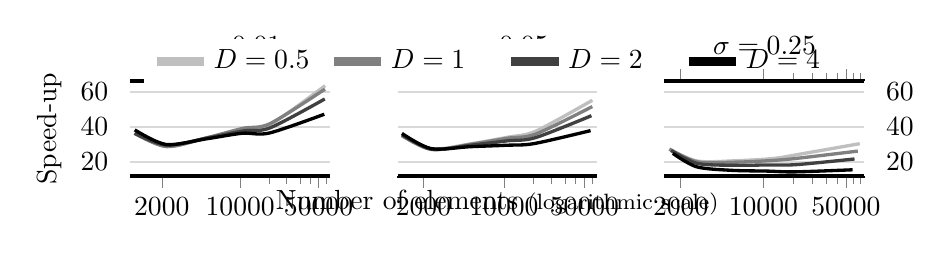
\begin{tikzpicture}
\begin{scope}[shift={(0.0\linewidth,0)}]
\begin{axis}[
 width=0.34\linewidth,height=0.23\linewidth,
 title=\normalsize\mbox{$\sigma=0.01$},
 xmode=log,enlarge x limits=0.025,
 ylabel=Speed-up,
 axis y line*=left,
 ymin=11.6727451262,ymax=66.0907077262,
 tick align=outside,
 x axis line style = ultra thick,y axis line style={white},
 xtick={2000,10000,50000},xticklabels={2000,10000,50000},
 minor xtick={18000,26000,34000,42000,58000,66000}, every y tick/.style={white},ymajorgrids,grid style={gray!30,thick}]
\addplot[very thick,mark=none,smooth,color=black!25] table[] {
	1142.66433333 36.2897800776
	2190.331 28.7700165654
	5024.068 33.6092943201
	10557.4073333 38.7642733564
	18518.477 41.2486285483
	57160.1013333 63.4993761738
};
\addplot[very thick,mark=none,smooth,color=black!50] table[] {
	1142.66433333 36.2897800776
	2203.91966667 28.5963227223
	5019.90933333 33.6092943201
	10559.26 39.0416951895
	18496.2383333 41.7761950928
	56994.2803333 61.4995484552
};
\addplot[very thick,mark=none,smooth,color=black!75] table[] {
	1147.421 36.1727917473
	2198.01033333 29.3866328257
	5048.57 33.4748571429
	10575.013 37.5305695142
	18463.3696667 39.3203242902
	56796.2563333 55.8640439053
};
\addplot[very thick,mark=none,smooth,color=black] table[] {
	1148.51366667 38.1659863946
	2179.72533333 29.8325221872
	4988.35566667 33.0443366426
	10445.26 36.2385050832
	18253.313 36.3940358628
	56234.555 47.1214037892
};
!\end{axis}
\end{scope}
\begin{scope}[shift={(0.28\linewidth,0)}]
\begin{axis}[
 width=0.34\linewidth,height=0.23\linewidth,
 title=\normalsize\mbox{$\sigma=0.05$},
 xmode=log,enlarge x limits=0.025,
 xlabel=Number of elements \footnotesize(logarithmic scale),x label style={at={(axis description cs:0.5,-0.05)},anchor=north},
 yticklabels={},
 legend style={at={(0.55,1.45)},legend style={text width=4em},legend style={draw=none},anchor=north,legend columns=-1},
 axis y line*=left,
 ymin=11.6727451262,ymax=66.0907077262,
 tick align=outside,
 x axis line style = ultra thick,y axis line style={white},
 xtick={2000,10000,50000},xticklabels={2000,10000,50000},
 minor xtick={18000,26000,34000,42000,58000,66000}, every y tick/.style={white},ymajorgrids,grid style={gray!30,thick}]
\addlegendimage{line width=3pt,mark=none,black!25}
\addlegendentry{$D=0.5$}
\addlegendimage{line width=3pt,mark=none,black!50}
\addlegendentry{$D=1$}
\addlegendimage{line width=3pt,mark=none,black!75}
\addlegendentry{$D=2$}
\addlegendimage{line width=3pt,mark=none,black}
\addlegendentry{$D=4$}
\addplot[very thick,mark=none,smooth,color=black!25] table[] {
	1298.20533333 34.9249530957
	2340.633 27.2511798637
	5186.95033333 30.2464011768
	10853.1023333 34.0036383991
	18943.9993333 37.479457559
	58604.5323333 55.1570578358
};
\addplot[very thick,mark=none,smooth,color=black!50] table[] {
	1297.63266667 34.903125
	2349.96633333 26.9194509195
	5211.535 29.9973947478
	10822.068 33.4383772775
	18923.0946667 35.8195142245
	58453.4236667 51.5111855511
};
\addplot[very thick,mark=none,smooth,color=black!75] table[] {
	1302.89433333 35.4346446701
	2349.60333333 27.1302531976
	5219.07066667 29.4661684922
	10751.7493333 31.9152569087
	18721.5463333 33.7135628445
	57464.189 46.2930500561
};
\addplot[very thick,mark=none,smooth,color=black] table[] {
	1299.731 36.145631068
	2327.66833333 27.4599735799
	5087.395 28.5513786947
	10536.52 29.375
	18361.0733333 30.3578422066
	56479.5 37.7507056018
};
!\end{axis}
\end{scope}
\begin{scope}[shift={(0.56\linewidth,0)}]
\begin{axis}[
 width=0.34\linewidth,height=0.23\linewidth,
 title=\normalsize\mbox{$\sigma=0.25$},
 xmode=log,enlarge x limits=0.025,
 axis y line*=right,
 ymin=11.6727451262,ymax=66.0907077262,
 tick align=outside,
 x axis line style = ultra thick,y axis line style={white},
 xtick={2000,10000,50000},xticklabels={2000,10000,50000},
 minor xtick={18000,26000,34000,42000,58000,66000}, every y tick/.style={white},ymajorgrids,grid style={gray!30,thick}]
\addplot[very thick,mark=none,smooth,color=black!25] table[] {
	1596.30333333 27.2734915925
	2756.53766667 20.3341269841
	6060.21733333 20.5562134613
	12338.161 21.8514300457
	21383.8163333 24.5252219532
	65427.1206667 30.2779874294
};
\addplot[very thick,mark=none,smooth,color=black!50] table[] {
	1607.67666667 27.1392716535
	2757.58366667 19.8998058252
	5836.15333333 19.7054892944
	11813.4666667 20.6324343136
	20455.343 22.0838397093
	63005.4993333 26.0327366598
};
\addplot[very thick,mark=none,smooth,color=black!75] table[] {
	1656.74966667 26.3861244019
	2746.29366667 19.0243178021
	5559.30066667 17.9208703607
	11210.0 18.1140543844
	19330.474 18.3126255524
	59102.68 21.5156095705
};
\addplot[very thick,mark=none,smooth,color=black] table[] {
	1714.92766667 24.7185118781
	2716.32133333 17.0579227696
	5316.24133333 15.0370634355
	10718.991 14.5844628668
	18519.036 14.140679938
	56886.458 15.3270226751
};
!\end{axis}
\end{scope}
\end{tikzpicture}
\end{center}
\caption{Speed-up results by mesh remodelling relative to mesh generation}
\centering\sffamily\footnotesize
Average of thirty optimisation scenarios - RAE-2822 airfoil
\end{figure}


\begin{figure}[!h]
\begin{center}
%	\input{figures/mesh_d1}
%	\input{figures/mesh_d4}
\begin{subfigure}{0.49\linewidth}
	\includegraphics[width=\linewidth]{pictures/mesh_d1}
	\caption{$D=1$}
\end{subfigure}
\hspace{0.01\linewidth}
\begin{subfigure}{0.49\linewidth}
	\includegraphics[width=\linewidth]{pictures/mesh_d4}
	\caption{$D=4$}
\end{subfigure}
\end{center}
\caption{Illustration of element surplus and bad gradation\\\footnotesize Mesh remodelling, $\sigma=0.25, I=400, G=8$, RAE-2822 airfoil}
\end{figure}

\paragraph{Improvements} Despite the good results, there is still room for improvement, especially concerning the problem of element surplus and bad gradation. One possible strategy, that follows from a previous work where its development and testing was carried out, involves choosing which method to perform --- generation or remodelling --- at a given iteration. The criteria for such decision can include the variation in the shape coefficient vector, $A$, the current value of element surplus --- although difficult to control, given that there is no point of comparison and that the higher number of elements could just be a consequence of a thinner model --- or even be a periodic event. One other alternative is as follows.
\begin{itemize}
\item In this work's particular case, due to the way the CMA-ES works, it is almost certain that at some point during the nine thousand iterations --- depending on the value of $\sigma$ --- the mesh remodelling method will start performing only full adjustments (adjust  all vertices) until the very end. One can take advantage of such behaviour and upon detecting, for example, ten successive full adjustments, instruct the program to perform a single mesh generation iteration. Since the remaining iterations are bound to be full adjustments, it is guaranteed that no elements will be either added or removed from the mesh, which results in an element surplus of 0\% from that point onwards at the cost of a merely one-hundredth of a percent in element preservation in the end.
\end{itemize}
Additionally, it is perfectly possible to opt for mesh deformation rather than mesh remodelling if it turns out to be more efficient on such small model perturbations --- although the only gain would be in speed-up. Ultimately, all possible improvements are to be considered from the fluid-dynamics simulator's point of view.
\section{Conclusions and Further developments}

\todo[inline]{}
\nocite{*}
\bibliography{references}
\appendix
\renewcommand*{\thefigure}{A\arabic{figure}}
\setcounter{figure}{0} 
\renewcommand*{\thetable}{A\arabic{table}}
\setcounter{table}{0} 

\newpage
\section{Appendix}

\subsection{Airfoils}
\begin{center}
\begin{minipage}[b]{0.49\linewidth}
	\begin{center}
		\begin{tikzpicture}[gnuplot, scale=0.7]
%% generated with GNUPLOT 5.0p5 (Lua 5.3; terminal rev. 99, script rev. 100)
%% Mon 23 Jan 2017 01:56:11 AM WET
%\path (0.000,0.000) rectangle (12.500,8.750);
\gpcolor{rgb color={0.533,0.533,0.533}}
\gpsetlinetype{gp lt border}
\gpsetdashtype{gp dt solid}
\gpsetlinewidth{2.00}
\draw[gp path] (11.947,4.375)--(11.924,4.375)--(11.901,4.375)--(11.878,4.375)--(11.855,4.375)%
--(11.832,4.375)--(11.809,4.375)--(11.786,4.375)--(11.763,4.375)--(11.740,4.375)--(11.717,4.375)%
--(11.694,4.375)--(11.671,4.375)--(11.648,4.375)--(11.625,4.375)--(11.602,4.375)--(11.579,4.375)%
--(11.556,4.375)--(11.533,4.375)--(11.510,4.375)--(11.488,4.375)--(11.465,4.375)--(11.442,4.375)%
--(11.419,4.375)--(11.396,4.375)--(11.373,4.375)--(11.350,4.375)--(11.327,4.375)--(11.304,4.375)%
--(11.281,4.375)--(11.258,4.375)--(11.235,4.375)--(11.212,4.375)--(11.189,4.375)--(11.166,4.375)%
--(11.143,4.375)--(11.120,4.375)--(11.097,4.375)--(11.074,4.375)--(11.051,4.375)--(11.028,4.375)%
--(11.005,4.375)--(10.982,4.375)--(10.959,4.375)--(10.936,4.375)--(10.913,4.375)--(10.890,4.375)%
--(10.867,4.375)--(10.844,4.375)--(10.821,4.375)--(10.798,4.375)--(10.775,4.375)--(10.752,4.375)%
--(10.729,4.375)--(10.706,4.375)--(10.683,4.375)--(10.660,4.375)--(10.637,4.375)--(10.615,4.375)%
--(10.592,4.375)--(10.569,4.375)--(10.546,4.375)--(10.523,4.375)--(10.500,4.375)--(10.477,4.375)%
--(10.454,4.375)--(10.431,4.375)--(10.408,4.375)--(10.385,4.375)--(10.362,4.375)--(10.339,4.375)%
--(10.316,4.375)--(10.293,4.375)--(10.270,4.375)--(10.247,4.375)--(10.224,4.375)--(10.201,4.375)%
--(10.178,4.375)--(10.155,4.375)--(10.132,4.375)--(10.109,4.375)--(10.086,4.375)--(10.063,4.375)%
--(10.040,4.375)--(10.017,4.375)--(9.994,4.375)--(9.971,4.375)--(9.948,4.375)--(9.925,4.375)%
--(9.902,4.375)--(9.879,4.375)--(9.856,4.375)--(9.833,4.375)--(9.810,4.375)--(9.787,4.375)%
--(9.764,4.375)--(9.741,4.375)--(9.719,4.375)--(9.696,4.375)--(9.673,4.375)--(9.650,4.375)%
--(9.627,4.375)--(9.604,4.375)--(9.581,4.375)--(9.558,4.375)--(9.535,4.375)--(9.512,4.375)%
--(9.489,4.375)--(9.466,4.375)--(9.443,4.375)--(9.420,4.375)--(9.397,4.375)--(9.374,4.375)%
--(9.351,4.375)--(9.328,4.375)--(9.305,4.375)--(9.282,4.375)--(9.259,4.375)--(9.236,4.375)%
--(9.213,4.375)--(9.190,4.375)--(9.167,4.375)--(9.144,4.375)--(9.121,4.375)--(9.098,4.375)%
--(9.075,4.375)--(9.052,4.375)--(9.029,4.375)--(9.006,4.375)--(8.983,4.375)--(8.960,4.375)%
--(8.937,4.375)--(8.914,4.375)--(8.891,4.375)--(8.868,4.375)--(8.846,4.375)--(8.823,4.375)%
--(8.800,4.375)--(8.777,4.375)--(8.754,4.375)--(8.731,4.375)--(8.708,4.375)--(8.685,4.375)%
--(8.662,4.375)--(8.639,4.375)--(8.616,4.375)--(8.593,4.375)--(8.570,4.375)--(8.547,4.375)%
--(8.524,4.375)--(8.501,4.375)--(8.478,4.375)--(8.455,4.375)--(8.432,4.375)--(8.409,4.375)%
--(8.386,4.375)--(8.363,4.375)--(8.340,4.375)--(8.317,4.375)--(8.294,4.375)--(8.271,4.375)%
--(8.248,4.375)--(8.225,4.375)--(8.202,4.375)--(8.179,4.375)--(8.156,4.375)--(8.133,4.375)%
--(8.110,4.375)--(8.087,4.375)--(8.064,4.375)--(8.041,4.375)--(8.018,4.375)--(7.995,4.375)%
--(7.972,4.375)--(7.950,4.375)--(7.927,4.375)--(7.904,4.375)--(7.881,4.375)--(7.858,4.375)%
--(7.835,4.375)--(7.812,4.375)--(7.789,4.375)--(7.766,4.375)--(7.743,4.375)--(7.720,4.375)%
--(7.697,4.375)--(7.674,4.375)--(7.651,4.375)--(7.628,4.375)--(7.605,4.375)--(7.582,4.375)%
--(7.559,4.375)--(7.536,4.375)--(7.513,4.375)--(7.490,4.375)--(7.467,4.375)--(7.444,4.375)%
--(7.421,4.375)--(7.398,4.375)--(7.375,4.375)--(7.352,4.375)--(7.329,4.375)--(7.306,4.375)%
--(7.283,4.375)--(7.260,4.375)--(7.237,4.375)--(7.214,4.375)--(7.191,4.375)--(7.168,4.375)%
--(7.145,4.375)--(7.122,4.375)--(7.099,4.375)--(7.077,4.375)--(7.054,4.375)--(7.031,4.375)%
--(7.008,4.375)--(6.985,4.375)--(6.962,4.375)--(6.939,4.375)--(6.916,4.375)--(6.893,4.375)%
--(6.870,4.375)--(6.847,4.375)--(6.824,4.375)--(6.801,4.375)--(6.778,4.375)--(6.755,4.375)%
--(6.732,4.375)--(6.709,4.375)--(6.686,4.375)--(6.663,4.375)--(6.640,4.375)--(6.617,4.375)%
--(6.594,4.375)--(6.571,4.375)--(6.548,4.375)--(6.525,4.375)--(6.502,4.375)--(6.479,4.375)%
--(6.456,4.375)--(6.433,4.375)--(6.410,4.375)--(6.387,4.375)--(6.364,4.375)--(6.341,4.375)%
--(6.318,4.375)--(6.295,4.375)--(6.272,4.375)--(6.249,4.375)--(6.226,4.375)--(6.204,4.375)%
--(6.181,4.375)--(6.158,4.375)--(6.135,4.375)--(6.112,4.375)--(6.089,4.375)--(6.066,4.375)%
--(6.043,4.375)--(6.020,4.375)--(5.997,4.375)--(5.974,4.375)--(5.951,4.375)--(5.928,4.375)%
--(5.905,4.375)--(5.882,4.375)--(5.859,4.375)--(5.836,4.375)--(5.813,4.375)--(5.790,4.375)%
--(5.767,4.375)--(5.744,4.375)--(5.721,4.375)--(5.698,4.375)--(5.675,4.375)--(5.652,4.375)%
--(5.629,4.375)--(5.606,4.375)--(5.583,4.375)--(5.560,4.375)--(5.537,4.375)--(5.514,4.375)%
--(5.491,4.375)--(5.468,4.375)--(5.445,4.375)--(5.422,4.375)--(5.399,4.375)--(5.376,4.375)%
--(5.353,4.375)--(5.330,4.375)--(5.308,4.375)--(5.285,4.375)--(5.262,4.375)--(5.239,4.375)%
--(5.216,4.375)--(5.193,4.375)--(5.170,4.375)--(5.147,4.375)--(5.124,4.375)--(5.101,4.375)%
--(5.078,4.375)--(5.055,4.375)--(5.032,4.375)--(5.009,4.375)--(4.986,4.375)--(4.963,4.375)%
--(4.940,4.375)--(4.917,4.375)--(4.894,4.375)--(4.871,4.375)--(4.848,4.375)--(4.825,4.375)%
--(4.802,4.375)--(4.779,4.375)--(4.756,4.375)--(4.733,4.375)--(4.710,4.375)--(4.687,4.375)%
--(4.664,4.375)--(4.641,4.375)--(4.618,4.375)--(4.595,4.375)--(4.572,4.375)--(4.549,4.375)%
--(4.526,4.375)--(4.503,4.375)--(4.480,4.375)--(4.457,4.375)--(4.435,4.375)--(4.412,4.375)%
--(4.389,4.375)--(4.366,4.375)--(4.343,4.375)--(4.320,4.375)--(4.297,4.375)--(4.274,4.375)%
--(4.251,4.375)--(4.228,4.375)--(4.205,4.375)--(4.182,4.375)--(4.159,4.375)--(4.136,4.375)%
--(4.113,4.375)--(4.090,4.375)--(4.067,4.375)--(4.044,4.375)--(4.021,4.375)--(3.998,4.375)%
--(3.975,4.375)--(3.952,4.375)--(3.929,4.375)--(3.906,4.375)--(3.883,4.375)--(3.860,4.375)%
--(3.837,4.375)--(3.814,4.375)--(3.791,4.375)--(3.768,4.375)--(3.745,4.375)--(3.722,4.375)%
--(3.699,4.375)--(3.676,4.375)--(3.653,4.375)--(3.630,4.375)--(3.607,4.375)--(3.584,4.375)%
--(3.561,4.375)--(3.539,4.375)--(3.516,4.375)--(3.493,4.375)--(3.470,4.375)--(3.447,4.375)%
--(3.424,4.375)--(3.401,4.375)--(3.378,4.375)--(3.355,4.375)--(3.332,4.375)--(3.309,4.375)%
--(3.286,4.375)--(3.263,4.375)--(3.240,4.375)--(3.217,4.375)--(3.194,4.375)--(3.171,4.375)%
--(3.148,4.375)--(3.125,4.375)--(3.102,4.375)--(3.079,4.375)--(3.056,4.375)--(3.033,4.375)%
--(3.010,4.375)--(2.987,4.375)--(2.964,4.375)--(2.941,4.375)--(2.918,4.375)--(2.895,4.375)%
--(2.872,4.375)--(2.849,4.375)--(2.826,4.375)--(2.803,4.375)--(2.780,4.375)--(2.757,4.375)%
--(2.734,4.375)--(2.711,4.375)--(2.688,4.375)--(2.666,4.375)--(2.643,4.375)--(2.620,4.375)%
--(2.597,4.375)--(2.574,4.375)--(2.551,4.375)--(2.528,4.375)--(2.505,4.375)--(2.482,4.375)%
--(2.459,4.375)--(2.436,4.375)--(2.413,4.375)--(2.390,4.375)--(2.367,4.375)--(2.344,4.375)%
--(2.321,4.375)--(2.298,4.375)--(2.275,4.375)--(2.252,4.375)--(2.229,4.375)--(2.206,4.375)%
--(2.183,4.375)--(2.160,4.375)--(2.137,4.375)--(2.114,4.375)--(2.091,4.375)--(2.068,4.375)%
--(2.045,4.375)--(2.022,4.375)--(1.999,4.375)--(1.976,4.375)--(1.953,4.375)--(1.930,4.375)%
--(1.907,4.375)--(1.884,4.375)--(1.861,4.375)--(1.838,4.375)--(1.815,4.375)--(1.792,4.375)%
--(1.770,4.375)--(1.747,4.375)--(1.724,4.375)--(1.701,4.375)--(1.678,4.375)--(1.655,4.375)%
--(1.632,4.375)--(1.609,4.375)--(1.586,4.375)--(1.563,4.375)--(1.540,4.375)--(1.517,4.375)%
--(1.494,4.375)--(1.471,4.375)--(1.448,4.375)--(1.425,4.375)--(1.402,4.375)--(1.379,4.375)%
--(1.356,4.375)--(1.333,4.375)--(1.310,4.375)--(1.287,4.375)--(1.264,4.375)--(1.241,4.375)%
--(1.218,4.375)--(1.195,4.375)--(1.172,4.375)--(1.149,4.375)--(1.126,4.375)--(1.103,4.375)%
--(1.080,4.375)--(1.057,4.375)--(1.034,4.375)--(1.011,4.375)--(0.988,4.375)--(0.965,4.375)%
--(0.942,4.375)--(0.919,4.375)--(0.897,4.375)--(0.874,4.375)--(0.851,4.375)--(0.828,4.375)%
--(0.805,4.375)--(0.782,4.375)--(0.759,4.375)--(0.736,4.375)--(0.713,4.375)--(0.690,4.375)%
--(0.667,4.375)--(0.644,4.375)--(0.621,4.375)--(0.598,4.375)--(0.575,4.375)--(0.552,4.375)%
--(0.529,4.375)--(0.506,4.375)--(0.483,4.375)--(0.460,4.375);
\gpcolor{rgb color={0.000,0.000,0.000}}
\draw[gp path] (11.947,4.375)--(11.924,4.378)--(11.901,4.381)--(11.878,4.384)--(11.855,4.387)%
--(11.832,4.390)--(11.809,4.394)--(11.786,4.397)--(11.763,4.400)--(11.740,4.403)--(11.717,4.406)%
--(11.694,4.409)--(11.671,4.413)--(11.648,4.416)--(11.625,4.419)--(11.602,4.422)--(11.579,4.425)%
--(11.556,4.428)--(11.533,4.431)--(11.510,4.434)--(11.488,4.437)--(11.465,4.441)--(11.442,4.444)%
--(11.419,4.447)--(11.396,4.450)--(11.373,4.453)--(11.350,4.456)--(11.327,4.459)--(11.304,4.462)%
--(11.281,4.465)--(11.258,4.468)--(11.235,4.471)--(11.212,4.474)--(11.189,4.477)--(11.166,4.480)%
--(11.143,4.483)--(11.120,4.486)--(11.097,4.489)--(11.074,4.492)--(11.051,4.495)--(11.028,4.498)%
--(11.005,4.500)--(10.982,4.503)--(10.959,4.506)--(10.936,4.509)--(10.913,4.512)--(10.890,4.515)%
--(10.867,4.518)--(10.844,4.521)--(10.821,4.524)--(10.798,4.527)--(10.775,4.529)--(10.752,4.532)%
--(10.729,4.535)--(10.706,4.538)--(10.683,4.541)--(10.660,4.544)--(10.637,4.546)--(10.615,4.549)%
--(10.592,4.552)--(10.569,4.555)--(10.546,4.558)--(10.523,4.560)--(10.500,4.563)--(10.477,4.566)%
--(10.454,4.569)--(10.431,4.571)--(10.408,4.574)--(10.385,4.577)--(10.362,4.580)--(10.339,4.582)%
--(10.316,4.585)--(10.293,4.588)--(10.270,4.591)--(10.247,4.593)--(10.224,4.596)--(10.201,4.599)%
--(10.178,4.601)--(10.155,4.604)--(10.132,4.607)--(10.109,4.609)--(10.086,4.612)--(10.063,4.615)%
--(10.040,4.617)--(10.017,4.620)--(9.994,4.623)--(9.971,4.625)--(9.948,4.628)--(9.925,4.631)%
--(9.902,4.633)--(9.879,4.636)--(9.856,4.638)--(9.833,4.641)--(9.810,4.644)--(9.787,4.646)%
--(9.764,4.649)--(9.741,4.651)--(9.719,4.654)--(9.696,4.656)--(9.673,4.659)--(9.650,4.661)%
--(9.627,4.664)--(9.604,4.667)--(9.581,4.669)--(9.558,4.672)--(9.535,4.674)--(9.512,4.677)%
--(9.489,4.679)--(9.466,4.682)--(9.443,4.684)--(9.420,4.687)--(9.397,4.689)--(9.374,4.692)%
--(9.351,4.694)--(9.328,4.697)--(9.305,4.699)--(9.282,4.702)--(9.259,4.704)--(9.236,4.706)%
--(9.213,4.709)--(9.190,4.711)--(9.167,4.714)--(9.144,4.716)--(9.121,4.719)--(9.098,4.721)%
--(9.075,4.723)--(9.052,4.726)--(9.029,4.728)--(9.006,4.731)--(8.983,4.733)--(8.960,4.735)%
--(8.937,4.738)--(8.914,4.740)--(8.891,4.743)--(8.868,4.745)--(8.846,4.747)--(8.823,4.750)%
--(8.800,4.752)--(8.777,4.754)--(8.754,4.757)--(8.731,4.759)--(8.708,4.761)--(8.685,4.764)%
--(8.662,4.766)--(8.639,4.768)--(8.616,4.771)--(8.593,4.773)--(8.570,4.775)--(8.547,4.778)%
--(8.524,4.780)--(8.501,4.782)--(8.478,4.784)--(8.455,4.787)--(8.432,4.789)--(8.409,4.791)%
--(8.386,4.793)--(8.363,4.796)--(8.340,4.798)--(8.317,4.800)--(8.294,4.802)--(8.271,4.805)%
--(8.248,4.807)--(8.225,4.809)--(8.202,4.811)--(8.179,4.813)--(8.156,4.816)--(8.133,4.818)%
--(8.110,4.820)--(8.087,4.822)--(8.064,4.824)--(8.041,4.826)--(8.018,4.829)--(7.995,4.831)%
--(7.972,4.833)--(7.950,4.835)--(7.927,4.837)--(7.904,4.839)--(7.881,4.841)--(7.858,4.844)%
--(7.835,4.846)--(7.812,4.848)--(7.789,4.850)--(7.766,4.852)--(7.743,4.854)--(7.720,4.856)%
--(7.697,4.858)--(7.674,4.860)--(7.651,4.862)--(7.628,4.864)--(7.605,4.866)--(7.582,4.868)%
--(7.559,4.870)--(7.536,4.872)--(7.513,4.874)--(7.490,4.876)--(7.467,4.878)--(7.444,4.880)%
--(7.421,4.882)--(7.398,4.884)--(7.375,4.886)--(7.352,4.888)--(7.329,4.890)--(7.306,4.892)%
--(7.283,4.894)--(7.260,4.896)--(7.237,4.898)--(7.214,4.900)--(7.191,4.902)--(7.168,4.904)%
--(7.145,4.906)--(7.122,4.907)--(7.099,4.909)--(7.077,4.911)--(7.054,4.913)--(7.031,4.915)%
--(7.008,4.917)--(6.985,4.919)--(6.962,4.920)--(6.939,4.922)--(6.916,4.924)--(6.893,4.926)%
--(6.870,4.928)--(6.847,4.929)--(6.824,4.931)--(6.801,4.933)--(6.778,4.935)--(6.755,4.936)%
--(6.732,4.938)--(6.709,4.940)--(6.686,4.942)--(6.663,4.943)--(6.640,4.945)--(6.617,4.947)%
--(6.594,4.948)--(6.571,4.950)--(6.548,4.952)--(6.525,4.953)--(6.502,4.955)--(6.479,4.957)%
--(6.456,4.958)--(6.433,4.960)--(6.410,4.961)--(6.387,4.963)--(6.364,4.965)--(6.341,4.966)%
--(6.318,4.968)--(6.295,4.969)--(6.272,4.971)--(6.249,4.972)--(6.226,4.974)--(6.204,4.975)%
--(6.181,4.977)--(6.158,4.978)--(6.135,4.980)--(6.112,4.981)--(6.089,4.983)--(6.066,4.984)%
--(6.043,4.985)--(6.020,4.987)--(5.997,4.988)--(5.974,4.990)--(5.951,4.991)--(5.928,4.992)%
--(5.905,4.994)--(5.882,4.995)--(5.859,4.996)--(5.836,4.998)--(5.813,4.999)--(5.790,5.000)%
--(5.767,5.002)--(5.744,5.003)--(5.721,5.004)--(5.698,5.005)--(5.675,5.007)--(5.652,5.008)%
--(5.629,5.009)--(5.606,5.010)--(5.583,5.011)--(5.560,5.013)--(5.537,5.014)--(5.514,5.015)%
--(5.491,5.016)--(5.468,5.017)--(5.445,5.018)--(5.422,5.019)--(5.399,5.020)--(5.376,5.021)%
--(5.353,5.023)--(5.330,5.024)--(5.308,5.025)--(5.285,5.026)--(5.262,5.027)--(5.239,5.028)%
--(5.216,5.029)--(5.193,5.029)--(5.170,5.030)--(5.147,5.031)--(5.124,5.032)--(5.101,5.033)%
--(5.078,5.034)--(5.055,5.035)--(5.032,5.036)--(5.009,5.037)--(4.986,5.037)--(4.963,5.038)%
--(4.940,5.039)--(4.917,5.040)--(4.894,5.041)--(4.871,5.041)--(4.848,5.042)--(4.825,5.043)%
--(4.802,5.043)--(4.779,5.044)--(4.756,5.045)--(4.733,5.045)--(4.710,5.046)--(4.687,5.047)%
--(4.664,5.047)--(4.641,5.048)--(4.618,5.048)--(4.595,5.049)--(4.572,5.049)--(4.549,5.050)%
--(4.526,5.050)--(4.503,5.051)--(4.480,5.051)--(4.457,5.052)--(4.435,5.052)--(4.412,5.053)%
--(4.389,5.053)--(4.366,5.053)--(4.343,5.054)--(4.320,5.054)--(4.297,5.054)--(4.274,5.055)%
--(4.251,5.055)--(4.228,5.055)--(4.205,5.056)--(4.182,5.056)--(4.159,5.056)--(4.136,5.056)%
--(4.113,5.056)--(4.090,5.056)--(4.067,5.057)--(4.044,5.057)--(4.021,5.057)--(3.998,5.057)%
--(3.975,5.057)--(3.952,5.057)--(3.929,5.057)--(3.906,5.057)--(3.883,5.057)--(3.860,5.057)%
--(3.837,5.057)--(3.814,5.057)--(3.791,5.057)--(3.768,5.057)--(3.745,5.056)--(3.722,5.056)%
--(3.699,5.056)--(3.676,5.056)--(3.653,5.056)--(3.630,5.055)--(3.607,5.055)--(3.584,5.055)%
--(3.561,5.054)--(3.539,5.054)--(3.516,5.054)--(3.493,5.053)--(3.470,5.053)--(3.447,5.052)%
--(3.424,5.052)--(3.401,5.051)--(3.378,5.051)--(3.355,5.050)--(3.332,5.050)--(3.309,5.049)%
--(3.286,5.049)--(3.263,5.048)--(3.240,5.047)--(3.217,5.047)--(3.194,5.046)--(3.171,5.045)%
--(3.148,5.044)--(3.125,5.044)--(3.102,5.043)--(3.079,5.042)--(3.056,5.041)--(3.033,5.040)%
--(3.010,5.039)--(2.987,5.038)--(2.964,5.037)--(2.941,5.036)--(2.918,5.035)--(2.895,5.034)%
--(2.872,5.033)--(2.849,5.032)--(2.826,5.031)--(2.803,5.029)--(2.780,5.028)--(2.757,5.027)%
--(2.734,5.026)--(2.711,5.024)--(2.688,5.023)--(2.666,5.022)--(2.643,5.020)--(2.620,5.019)%
--(2.597,5.017)--(2.574,5.016)--(2.551,5.014)--(2.528,5.012)--(2.505,5.011)--(2.482,5.009)%
--(2.459,5.007)--(2.436,5.006)--(2.413,5.004)--(2.390,5.002)--(2.367,5.000)--(2.344,4.998)%
--(2.321,4.996)--(2.298,4.994)--(2.275,4.992)--(2.252,4.990)--(2.229,4.988)--(2.206,4.986)%
--(2.183,4.983)--(2.160,4.981)--(2.137,4.979)--(2.114,4.976)--(2.091,4.974)--(2.068,4.971)%
--(2.045,4.969)--(2.022,4.966)--(1.999,4.964)--(1.976,4.961)--(1.953,4.958)--(1.930,4.955)%
--(1.907,4.953)--(1.884,4.950)--(1.861,4.947)--(1.838,4.944)--(1.815,4.940)--(1.792,4.937)%
--(1.770,4.934)--(1.747,4.931)--(1.724,4.927)--(1.701,4.924)--(1.678,4.920)--(1.655,4.917)%
--(1.632,4.913)--(1.609,4.909)--(1.586,4.906)--(1.563,4.902)--(1.540,4.898)--(1.517,4.894)%
--(1.494,4.889)--(1.471,4.885)--(1.448,4.881)--(1.425,4.876)--(1.402,4.872)--(1.379,4.867)%
--(1.356,4.862)--(1.333,4.857)--(1.310,4.852)--(1.287,4.847)--(1.264,4.842)--(1.241,4.836)%
--(1.218,4.831)--(1.195,4.825)--(1.172,4.819)--(1.149,4.814)--(1.126,4.807)--(1.103,4.801)%
--(1.080,4.795)--(1.057,4.788)--(1.034,4.781)--(1.011,4.774)--(0.988,4.767)--(0.965,4.759)%
--(0.942,4.751)--(0.919,4.743)--(0.897,4.735)--(0.874,4.726)--(0.851,4.718)--(0.828,4.708)%
--(0.805,4.699)--(0.782,4.688)--(0.759,4.678)--(0.736,4.667)--(0.713,4.655)--(0.690,4.643)%
--(0.667,4.630)--(0.644,4.616)--(0.621,4.601)--(0.598,4.585)--(0.575,4.567)--(0.552,4.547)%
--(0.529,4.524)--(0.506,4.497)--(0.483,4.462)--(0.460,4.375)--(0.483,4.287)--(0.506,4.252)%
--(0.529,4.225)--(0.552,4.202)--(0.575,4.182)--(0.598,4.164)--(0.621,4.148)--(0.644,4.133)%
--(0.667,4.119)--(0.690,4.106)--(0.713,4.094)--(0.736,4.082)--(0.759,4.071)--(0.782,4.061)%
--(0.805,4.050)--(0.828,4.041)--(0.851,4.031)--(0.874,4.023)--(0.897,4.014)--(0.919,4.006)%
--(0.942,3.998)--(0.965,3.990)--(0.988,3.982)--(1.011,3.975)--(1.034,3.968)--(1.057,3.961)%
--(1.080,3.954)--(1.103,3.948)--(1.126,3.942)--(1.149,3.935)--(1.172,3.930)--(1.195,3.924)%
--(1.218,3.918)--(1.241,3.913)--(1.264,3.907)--(1.287,3.902)--(1.310,3.897)--(1.333,3.892)%
--(1.356,3.887)--(1.379,3.882)--(1.402,3.877)--(1.425,3.873)--(1.448,3.868)--(1.471,3.864)%
--(1.494,3.860)--(1.517,3.855)--(1.540,3.851)--(1.563,3.847)--(1.586,3.843)--(1.609,3.840)%
--(1.632,3.836)--(1.655,3.832)--(1.678,3.829)--(1.701,3.825)--(1.724,3.822)--(1.747,3.818)%
--(1.770,3.815)--(1.792,3.812)--(1.815,3.809)--(1.838,3.805)--(1.861,3.802)--(1.884,3.799)%
--(1.907,3.796)--(1.930,3.794)--(1.953,3.791)--(1.976,3.788)--(1.999,3.785)--(2.022,3.783)%
--(2.045,3.780)--(2.068,3.778)--(2.091,3.775)--(2.114,3.773)--(2.137,3.770)--(2.160,3.768)%
--(2.183,3.766)--(2.206,3.763)--(2.229,3.761)--(2.252,3.759)--(2.275,3.757)--(2.298,3.755)%
--(2.321,3.753)--(2.344,3.751)--(2.367,3.749)--(2.390,3.747)--(2.413,3.745)--(2.436,3.743)%
--(2.459,3.742)--(2.482,3.740)--(2.505,3.738)--(2.528,3.737)--(2.551,3.735)--(2.574,3.733)%
--(2.597,3.732)--(2.620,3.730)--(2.643,3.729)--(2.666,3.727)--(2.688,3.726)--(2.711,3.725)%
--(2.734,3.723)--(2.757,3.722)--(2.780,3.721)--(2.803,3.720)--(2.826,3.718)--(2.849,3.717)%
--(2.872,3.716)--(2.895,3.715)--(2.918,3.714)--(2.941,3.713)--(2.964,3.712)--(2.987,3.711)%
--(3.010,3.710)--(3.033,3.709)--(3.056,3.708)--(3.079,3.707)--(3.102,3.706)--(3.125,3.705)%
--(3.148,3.705)--(3.171,3.704)--(3.194,3.703)--(3.217,3.702)--(3.240,3.702)--(3.263,3.701)%
--(3.286,3.700)--(3.309,3.700)--(3.332,3.699)--(3.355,3.699)--(3.378,3.698)--(3.401,3.698)%
--(3.424,3.697)--(3.447,3.697)--(3.470,3.696)--(3.493,3.696)--(3.516,3.695)--(3.539,3.695)%
--(3.561,3.695)--(3.584,3.694)--(3.607,3.694)--(3.630,3.694)--(3.653,3.693)--(3.676,3.693)%
--(3.699,3.693)--(3.722,3.693)--(3.745,3.693)--(3.768,3.692)--(3.791,3.692)--(3.814,3.692)%
--(3.837,3.692)--(3.860,3.692)--(3.883,3.692)--(3.906,3.692)--(3.929,3.692)--(3.952,3.692)%
--(3.975,3.692)--(3.998,3.692)--(4.021,3.692)--(4.044,3.692)--(4.067,3.692)--(4.090,3.693)%
--(4.113,3.693)--(4.136,3.693)--(4.159,3.693)--(4.182,3.693)--(4.205,3.693)--(4.228,3.694)%
--(4.251,3.694)--(4.274,3.694)--(4.297,3.695)--(4.320,3.695)--(4.343,3.695)--(4.366,3.696)%
--(4.389,3.696)--(4.412,3.696)--(4.435,3.697)--(4.457,3.697)--(4.480,3.698)--(4.503,3.698)%
--(4.526,3.699)--(4.549,3.699)--(4.572,3.700)--(4.595,3.700)--(4.618,3.701)--(4.641,3.701)%
--(4.664,3.702)--(4.687,3.702)--(4.710,3.703)--(4.733,3.704)--(4.756,3.704)--(4.779,3.705)%
--(4.802,3.706)--(4.825,3.706)--(4.848,3.707)--(4.871,3.708)--(4.894,3.708)--(4.917,3.709)%
--(4.940,3.710)--(4.963,3.711)--(4.986,3.712)--(5.009,3.712)--(5.032,3.713)--(5.055,3.714)%
--(5.078,3.715)--(5.101,3.716)--(5.124,3.717)--(5.147,3.718)--(5.170,3.719)--(5.193,3.720)%
--(5.216,3.720)--(5.239,3.721)--(5.262,3.722)--(5.285,3.723)--(5.308,3.724)--(5.330,3.725)%
--(5.353,3.726)--(5.376,3.728)--(5.399,3.729)--(5.422,3.730)--(5.445,3.731)--(5.468,3.732)%
--(5.491,3.733)--(5.514,3.734)--(5.537,3.735)--(5.560,3.736)--(5.583,3.738)--(5.606,3.739)%
--(5.629,3.740)--(5.652,3.741)--(5.675,3.742)--(5.698,3.744)--(5.721,3.745)--(5.744,3.746)%
--(5.767,3.747)--(5.790,3.749)--(5.813,3.750)--(5.836,3.751)--(5.859,3.753)--(5.882,3.754)%
--(5.905,3.755)--(5.928,3.757)--(5.951,3.758)--(5.974,3.759)--(5.997,3.761)--(6.020,3.762)%
--(6.043,3.764)--(6.066,3.765)--(6.089,3.766)--(6.112,3.768)--(6.135,3.769)--(6.158,3.771)%
--(6.181,3.772)--(6.204,3.774)--(6.226,3.775)--(6.249,3.777)--(6.272,3.778)--(6.295,3.780)%
--(6.318,3.781)--(6.341,3.783)--(6.364,3.784)--(6.387,3.786)--(6.410,3.788)--(6.433,3.789)%
--(6.456,3.791)--(6.479,3.792)--(6.502,3.794)--(6.525,3.796)--(6.548,3.797)--(6.571,3.799)%
--(6.594,3.801)--(6.617,3.802)--(6.640,3.804)--(6.663,3.806)--(6.686,3.807)--(6.709,3.809)%
--(6.732,3.811)--(6.755,3.813)--(6.778,3.814)--(6.801,3.816)--(6.824,3.818)--(6.847,3.820)%
--(6.870,3.821)--(6.893,3.823)--(6.916,3.825)--(6.939,3.827)--(6.962,3.829)--(6.985,3.830)%
--(7.008,3.832)--(7.031,3.834)--(7.054,3.836)--(7.077,3.838)--(7.099,3.840)--(7.122,3.842)%
--(7.145,3.843)--(7.168,3.845)--(7.191,3.847)--(7.214,3.849)--(7.237,3.851)--(7.260,3.853)%
--(7.283,3.855)--(7.306,3.857)--(7.329,3.859)--(7.352,3.861)--(7.375,3.863)--(7.398,3.865)%
--(7.421,3.867)--(7.444,3.869)--(7.467,3.871)--(7.490,3.873)--(7.513,3.875)--(7.536,3.877)%
--(7.559,3.879)--(7.582,3.881)--(7.605,3.883)--(7.628,3.885)--(7.651,3.887)--(7.674,3.889)%
--(7.697,3.891)--(7.720,3.893)--(7.743,3.895)--(7.766,3.897)--(7.789,3.899)--(7.812,3.901)%
--(7.835,3.903)--(7.858,3.905)--(7.881,3.908)--(7.904,3.910)--(7.927,3.912)--(7.950,3.914)%
--(7.972,3.916)--(7.995,3.918)--(8.018,3.920)--(8.041,3.923)--(8.064,3.925)--(8.087,3.927)%
--(8.110,3.929)--(8.133,3.931)--(8.156,3.933)--(8.179,3.936)--(8.202,3.938)--(8.225,3.940)%
--(8.248,3.942)--(8.271,3.944)--(8.294,3.947)--(8.317,3.949)--(8.340,3.951)--(8.363,3.953)%
--(8.386,3.956)--(8.409,3.958)--(8.432,3.960)--(8.455,3.962)--(8.478,3.965)--(8.501,3.967)%
--(8.524,3.969)--(8.547,3.971)--(8.570,3.974)--(8.593,3.976)--(8.616,3.978)--(8.639,3.981)%
--(8.662,3.983)--(8.685,3.985)--(8.708,3.988)--(8.731,3.990)--(8.754,3.992)--(8.777,3.995)%
--(8.800,3.997)--(8.823,3.999)--(8.846,4.002)--(8.868,4.004)--(8.891,4.006)--(8.914,4.009)%
--(8.937,4.011)--(8.960,4.014)--(8.983,4.016)--(9.006,4.018)--(9.029,4.021)--(9.052,4.023)%
--(9.075,4.026)--(9.098,4.028)--(9.121,4.030)--(9.144,4.033)--(9.167,4.035)--(9.190,4.038)%
--(9.213,4.040)--(9.236,4.043)--(9.259,4.045)--(9.282,4.047)--(9.305,4.050)--(9.328,4.052)%
--(9.351,4.055)--(9.374,4.057)--(9.397,4.060)--(9.420,4.062)--(9.443,4.065)--(9.466,4.067)%
--(9.489,4.070)--(9.512,4.072)--(9.535,4.075)--(9.558,4.077)--(9.581,4.080)--(9.604,4.082)%
--(9.627,4.085)--(9.650,4.088)--(9.673,4.090)--(9.696,4.093)--(9.719,4.095)--(9.741,4.098)%
--(9.764,4.100)--(9.787,4.103)--(9.810,4.105)--(9.833,4.108)--(9.856,4.111)--(9.879,4.113)%
--(9.902,4.116)--(9.925,4.118)--(9.948,4.121)--(9.971,4.124)--(9.994,4.126)--(10.017,4.129)%
--(10.040,4.132)--(10.063,4.134)--(10.086,4.137)--(10.109,4.140)--(10.132,4.142)--(10.155,4.145)%
--(10.178,4.148)--(10.201,4.150)--(10.224,4.153)--(10.247,4.156)--(10.270,4.158)--(10.293,4.161)%
--(10.316,4.164)--(10.339,4.167)--(10.362,4.169)--(10.385,4.172)--(10.408,4.175)--(10.431,4.178)%
--(10.454,4.180)--(10.477,4.183)--(10.500,4.186)--(10.523,4.189)--(10.546,4.191)--(10.569,4.194)%
--(10.592,4.197)--(10.615,4.200)--(10.637,4.203)--(10.660,4.205)--(10.683,4.208)--(10.706,4.211)%
--(10.729,4.214)--(10.752,4.217)--(10.775,4.220)--(10.798,4.222)--(10.821,4.225)--(10.844,4.228)%
--(10.867,4.231)--(10.890,4.234)--(10.913,4.237)--(10.936,4.240)--(10.959,4.243)--(10.982,4.246)%
--(11.005,4.249)--(11.028,4.251)--(11.051,4.254)--(11.074,4.257)--(11.097,4.260)--(11.120,4.263)%
--(11.143,4.266)--(11.166,4.269)--(11.189,4.272)--(11.212,4.275)--(11.235,4.278)--(11.258,4.281)%
--(11.281,4.284)--(11.304,4.287)--(11.327,4.290)--(11.350,4.293)--(11.373,4.296)--(11.396,4.299)%
--(11.419,4.302)--(11.442,4.305)--(11.465,4.308)--(11.488,4.312)--(11.510,4.315)--(11.533,4.318)%
--(11.556,4.321)--(11.579,4.324)--(11.602,4.327)--(11.625,4.330)--(11.648,4.333)--(11.671,4.336)%
--(11.694,4.340)--(11.717,4.343)--(11.740,4.346)--(11.763,4.349)--(11.786,4.352)--(11.809,4.355)%
--(11.832,4.359)--(11.855,4.362)--(11.878,4.365)--(11.901,4.368)--(11.924,4.371)--cycle;
%% coordinates of the plot area
%\gpdefrectangularnode{gp plot 1}{\pgfpoint{0.460cm}{3.806cm}}{\pgfpoint{11.947cm}{4.943cm}}
\end{tikzpicture}\\[1pc]
%% gnuplot variables
\begin{tabular}{r l}
	Max. Thickness: & 12\% at 30\% of the chord \\
	Max. Camber: & 0
\end{tabular}
\captionof{figure}{NACA 0012}
\end{center}
\end{minipage}

\begin{minipage}[b]{0.49\linewidth}
	\begin{center}
		\begin{tikzpicture}[gnuplot, scale=0.84]
%% generated with GNUPLOT 5.0p5 (Lua 5.3; terminal rev. 99, script rev. 100)
%% Mon 23 Jan 2017 01:56:11 AM WET
%\path (0.000,0.000) rectangle (12.500,8.750);
\gpcolor{rgb color={0.533,0.533,0.533}}
\gpsetlinetype{gp lt border}
\gpsetdashtype{gp dt solid}
\gpsetlinewidth{2.00}
\draw[gp path] (10.990,4.374)--(10.989,4.374)--(10.988,4.374)--(10.987,4.374)--(10.986,4.374)%
  --(10.985,4.374)--(10.984,4.374)--(10.982,4.374)--(10.980,4.374)--(10.978,4.374)--(10.976,4.374)%
  --(10.974,4.374)--(10.971,4.374)--(10.969,4.374)--(10.966,4.374)--(10.962,4.374)--(10.959,4.374)%
  --(10.956,4.374)--(10.952,4.374)--(10.948,4.374)--(10.944,4.374)--(10.940,4.374)--(10.935,4.374)%
  --(10.931,4.374)--(10.926,4.374)--(10.921,4.374)--(10.916,4.374)--(10.911,4.374)--(10.905,4.374)%
  --(10.899,4.374)--(10.893,4.374)--(10.887,4.374)--(10.881,4.374)--(10.874,4.374)--(10.868,4.374)%
  --(10.861,4.374)--(10.854,4.374)--(10.847,4.374)--(10.839,4.374)--(10.832,4.374)--(10.824,4.374)%
  --(10.816,4.374)--(10.808,4.374)--(10.800,4.374)--(10.791,4.374)--(10.783,4.374)--(10.774,4.374)%
  --(10.765,4.374)--(10.755,4.374)--(10.746,4.374)--(10.737,4.374)--(10.727,4.374)--(10.717,4.374)%
  --(10.707,4.374)--(10.697,4.374)--(10.686,4.374)--(10.675,4.374)--(10.665,4.374)--(10.654,4.374)%
  --(10.642,4.374)--(10.631,4.374)--(10.620,4.374)--(10.608,4.374)--(10.596,4.374)--(10.584,4.374)%
  --(10.572,4.374)--(10.559,4.374)--(10.547,4.374)--(10.534,4.374)--(10.521,4.374)--(10.508,4.374)%
  --(10.495,4.374)--(10.482,4.374)--(10.468,4.374)--(10.454,4.374)--(10.440,4.374)--(10.426,4.374)%
  --(10.412,4.374)--(10.398,4.374)--(10.383,4.374)--(10.368,4.374)--(10.354,4.374)--(10.338,4.374)%
  --(10.323,4.374)--(10.308,4.374)--(10.292,4.374)--(10.277,4.374)--(10.261,4.374)--(10.245,4.374)%
  --(10.228,4.374)--(10.212,4.374)--(10.196,4.374)--(10.179,4.374)--(10.162,4.374)--(10.145,4.374)%
  --(10.128,4.374)--(10.111,4.374)--(10.093,4.374)--(10.076,4.374)--(10.058,4.374)--(10.040,4.374)%
  --(10.022,4.374)--(10.004,4.374)--(9.985,4.374)--(9.967,4.374)--(9.948,4.374)--(9.929,4.374)%
  --(9.910,4.374)--(9.891,4.374)--(9.872,4.374)--(9.853,4.374)--(9.833,4.374)--(9.814,4.374)%
  --(9.794,4.374)--(9.774,4.374)--(9.754,4.374)--(9.733,4.374)--(9.713,4.374)--(9.693,4.374)%
  --(9.672,4.374)--(9.651,4.374)--(9.630,4.374)--(9.609,4.374)--(9.588,4.374)--(9.567,4.374)%
  --(9.545,4.375)--(9.523,4.375)--(9.502,4.375)--(9.480,4.375)--(9.458,4.375)--(9.436,4.375)%
  --(9.414,4.375)--(9.391,4.375)--(9.369,4.375)--(9.346,4.375)--(9.323,4.375)--(9.300,4.375)%
  --(9.277,4.375)--(9.254,4.375)--(9.231,4.375)--(9.208,4.375)--(9.184,4.375)--(9.161,4.375)%
  --(9.137,4.375)--(9.113,4.375)--(9.089,4.375)--(9.065,4.375)--(9.041,4.375)--(9.017,4.375)%
  --(8.992,4.375)--(8.968,4.375)--(8.943,4.375)--(8.919,4.375)--(8.894,4.375)--(8.869,4.375)%
  --(8.844,4.375)--(8.819,4.375)--(8.793,4.375)--(8.768,4.375)--(8.743,4.375)--(8.717,4.375)%
  --(8.691,4.375)--(8.666,4.375)--(8.640,4.375)--(8.614,4.375)--(8.588,4.375)--(8.562,4.375)%
  --(8.536,4.375)--(8.509,4.375)--(8.483,4.375)--(8.456,4.375)--(8.430,4.375)--(8.403,4.375)%
  --(8.376,4.375)--(8.350,4.375)--(8.323,4.375)--(8.296,4.375)--(8.269,4.375)--(8.241,4.375)%
  --(8.214,4.374)--(8.187,4.374)--(8.159,4.374)--(8.132,4.374)--(8.104,4.374)--(8.077,4.374)%
  --(8.049,4.374)--(8.021,4.374)--(7.993,4.374)--(7.965,4.374)--(7.937,4.374)--(7.909,4.374)%
  --(7.881,4.374)--(7.853,4.374)--(7.825,4.374)--(7.796,4.374)--(7.768,4.374)--(7.740,4.374)%
  --(7.711,4.374)--(7.683,4.374)--(7.654,4.374)--(7.625,4.374)--(7.596,4.374)--(7.568,4.374)%
  --(7.539,4.374)--(7.510,4.374)--(7.481,4.374)--(7.452,4.374)--(7.423,4.374)--(7.394,4.374)%
  --(7.365,4.374)--(7.335,4.374)--(7.306,4.374)--(7.277,4.374)--(7.248,4.374)--(7.218,4.374)%
  --(7.189,4.374)--(7.159,4.374)--(7.130,4.374)--(7.100,4.374)--(7.071,4.374)--(7.041,4.374)%
  --(7.012,4.374)--(6.982,4.374)--(6.952,4.374)--(6.923,4.374)--(6.893,4.374)--(6.863,4.374)%
  --(6.833,4.374)--(6.803,4.374)--(6.774,4.374)--(6.744,4.374)--(6.714,4.374)--(6.684,4.374)%
  --(6.654,4.374)--(6.624,4.374)--(6.594,4.374)--(6.564,4.374)--(6.534,4.374)--(6.504,4.374)%
  --(6.474,4.374)--(6.444,4.374)--(6.414,4.374)--(6.384,4.374)--(6.354,4.374)--(6.324,4.374)%
  --(6.294,4.374)--(6.264,4.374)--(6.234,4.374)--(6.203,4.374)--(6.173,4.374)--(6.143,4.374)%
  --(6.113,4.374)--(6.083,4.374)--(6.053,4.374)--(6.023,4.374)--(5.993,4.374)--(5.963,4.374)%
  --(5.933,4.374)--(5.903,4.374)--(5.873,4.374)--(5.843,4.374)--(5.813,4.374)--(5.783,4.374)%
  --(5.753,4.374)--(5.723,4.374)--(5.693,4.374)--(5.663,4.374)--(5.633,4.374)--(5.604,4.374)%
  --(5.574,4.374)--(5.544,4.374)--(5.514,4.374)--(5.484,4.374)--(5.455,4.374)--(5.425,4.374)%
  --(5.395,4.374)--(5.366,4.374)--(5.336,4.374)--(5.307,4.374)--(5.277,4.374)--(5.248,4.374)%
  --(5.218,4.374)--(5.189,4.374)--(5.159,4.374)--(5.130,4.374)--(5.101,4.374)--(5.072,4.374)%
  --(5.042,4.374)--(5.013,4.374)--(4.984,4.374)--(4.955,4.374)--(4.926,4.374)--(4.897,4.374)%
  --(4.868,4.374)--(4.839,4.374)--(4.811,4.374)--(4.782,4.374)--(4.753,4.374)--(4.724,4.375)%
  --(4.696,4.375)--(4.667,4.375)--(4.639,4.375)--(4.611,4.375)--(4.582,4.375)--(4.554,4.374)%
  --(4.526,4.374)--(4.498,4.374)--(4.470,4.374)--(4.442,4.374)--(4.414,4.374)--(4.386,4.374)%
  --(4.358,4.374)--(4.330,4.374)--(4.303,4.374)--(4.275,4.374)--(4.248,4.374)--(4.220,4.374)%
  --(4.193,4.374)--(4.166,4.374)--(4.138,4.374)--(4.111,4.374)--(4.084,4.374)--(4.057,4.374)%
  --(4.031,4.374)--(4.004,4.374)--(3.977,4.374)--(3.951,4.374)--(3.924,4.374)--(3.898,4.374)%
  --(3.871,4.374)--(3.845,4.374)--(3.819,4.374)--(3.793,4.374)--(3.767,4.374)--(3.741,4.374)%
  --(3.716,4.374)--(3.690,4.374)--(3.664,4.374)--(3.639,4.374)--(3.614,4.374)--(3.588,4.374)%
  --(3.563,4.374)--(3.538,4.374)--(3.513,4.374)--(3.488,4.374)--(3.464,4.374)--(3.439,4.374)%
  --(3.415,4.374)--(3.390,4.374)--(3.366,4.374)--(3.342,4.374)--(3.318,4.374)--(3.294,4.374)%
  --(3.270,4.374)--(3.246,4.374)--(3.223,4.374)--(3.199,4.374)--(3.176,4.374)--(3.153,4.374)%
  --(3.130,4.374)--(3.107,4.374)--(3.084,4.374)--(3.061,4.374)--(3.038,4.374)--(3.016,4.374)%
  --(2.993,4.374)--(2.971,4.374)--(2.949,4.374)--(2.927,4.374)--(2.905,4.374)--(2.884,4.374)%
  --(2.862,4.374)--(2.840,4.374)--(2.819,4.374)--(2.798,4.374)--(2.777,4.374)--(2.756,4.374)%
  --(2.735,4.374)--(2.714,4.374)--(2.694,4.374)--(2.674,4.374)--(2.653,4.374)--(2.633,4.374)%
  --(2.613,4.374)--(2.593,4.374)--(2.574,4.374)--(2.554,4.374)--(2.535,4.374)--(2.516,4.374)%
  --(2.497,4.374)--(2.478,4.374)--(2.459,4.374)--(2.440,4.374)--(2.422,4.374)--(2.403,4.374)%
  --(2.385,4.374)--(2.367,4.374)--(2.349,4.374)--(2.331,4.374)--(2.314,4.374)--(2.296,4.374)%
  --(2.279,4.374)--(2.262,4.374)--(2.245,4.374)--(2.228,4.374)--(2.211,4.374)--(2.195,4.374)%
  --(2.179,4.374)--(2.162,4.374)--(2.146,4.374)--(2.130,4.374)--(2.115,4.374)--(2.099,4.374)%
  --(2.084,4.374)--(2.069,4.374)--(2.053,4.374)--(2.039,4.374)--(2.024,4.374)--(2.009,4.374)%
  --(1.995,4.374)--(1.981,4.374)--(1.967,4.374)--(1.953,4.374)--(1.939,4.374)--(1.925,4.374)%
  --(1.912,4.374)--(1.899,4.374)--(1.886,4.374)--(1.873,4.374)--(1.860,4.374)--(1.848,4.374)%
  --(1.835,4.374)--(1.823,4.374)--(1.811,4.374)--(1.799,4.374)--(1.787,4.374)--(1.776,4.374)%
  --(1.765,4.374)--(1.753,4.374)--(1.742,4.374)--(1.732,4.374)--(1.721,4.374)--(1.710,4.374)%
  --(1.700,4.374)--(1.690,4.374)--(1.680,4.374)--(1.670,4.374)--(1.661,4.374)--(1.652,4.374)%
  --(1.642,4.374)--(1.633,4.374)--(1.624,4.374)--(1.616,4.374)--(1.607,4.374)--(1.599,4.374)%
  --(1.591,4.374)--(1.583,4.374)--(1.575,4.374)--(1.568,4.374)--(1.560,4.374)--(1.553,4.374)%
  --(1.546,4.374)--(1.539,4.374)--(1.533,4.374)--(1.526,4.374)--(1.520,4.374)--(1.514,4.374)%
  --(1.508,4.374)--(1.502,4.374)--(1.496,4.374)--(1.491,4.374)--(1.486,4.374)--(1.481,4.374)%
  --(1.476,4.374)--(1.472,4.374)--(1.467,4.374)--(1.463,4.374)--(1.459,4.374)--(1.455,4.374)%
  --(1.451,4.374)--(1.448,4.374)--(1.445,4.374)--(1.441,4.374)--(1.438,4.374)--(1.436,4.374)%
  --(1.433,4.374)--(1.431,4.374)--(1.429,4.374)--(1.427,4.374)--(1.425,4.374)--(1.423,4.374)%
  --(1.422,4.374)--(1.421,4.374)--(1.420,4.374)--(1.419,4.374)--(1.418,4.374)--(1.417,4.374);
\gpcolor{rgb color={0.000,0.000,0.000}}
\draw[gp path] (10.990,4.374)--(10.990,4.375)--(10.989,4.375)--(10.988,4.375)--(10.987,4.375)%
  --(10.986,4.375)--(10.985,4.375)--(10.984,4.376)--(10.982,4.376)--(10.980,4.377)--(10.978,4.377)%
  --(10.976,4.377)--(10.974,4.378)--(10.971,4.378)--(10.969,4.379)--(10.966,4.380)--(10.962,4.380)%
  --(10.959,4.381)--(10.956,4.382)--(10.952,4.382)--(10.948,4.383)--(10.944,4.384)--(10.940,4.385)%
  --(10.935,4.386)--(10.931,4.387)--(10.926,4.388)--(10.921,4.389)--(10.916,4.390)--(10.911,4.391)%
  --(10.905,4.392)--(10.899,4.393)--(10.893,4.394)--(10.887,4.395)--(10.881,4.397)--(10.874,4.398)%
  --(10.868,4.399)--(10.861,4.400)--(10.854,4.402)--(10.847,4.403)--(10.839,4.405)--(10.832,4.406)%
  --(10.824,4.407)--(10.816,4.409)--(10.808,4.410)--(10.800,4.412)--(10.791,4.413)--(10.783,4.415)%
  --(10.774,4.417)--(10.765,4.418)--(10.755,4.420)--(10.746,4.421)--(10.737,4.423)--(10.727,4.425)%
  --(10.717,4.427)--(10.707,4.428)--(10.697,4.430)--(10.686,4.432)--(10.675,4.434)--(10.665,4.435)%
  --(10.654,4.437)--(10.642,4.439)--(10.631,4.441)--(10.620,4.443)--(10.608,4.445)--(10.596,4.447)%
  --(10.584,4.449)--(10.572,4.451)--(10.559,4.453)--(10.547,4.455)--(10.534,4.457)--(10.521,4.459)%
  --(10.508,4.461)--(10.495,4.463)--(10.482,4.465)--(10.468,4.467)--(10.454,4.469)--(10.440,4.471)%
  --(10.426,4.473)--(10.412,4.475)--(10.398,4.477)--(10.383,4.479)--(10.368,4.482)--(10.354,4.484)%
  --(10.338,4.486)--(10.323,4.488)--(10.308,4.490)--(10.292,4.493)--(10.277,4.495)--(10.261,4.497)%
  --(10.245,4.499)--(10.228,4.502)--(10.212,4.504)--(10.196,4.506)--(10.179,4.508)--(10.162,4.511)%
  --(10.145,4.513)--(10.128,4.515)--(10.111,4.518)--(10.093,4.520)--(10.076,4.523)--(10.058,4.525)%
  --(10.040,4.527)--(10.022,4.530)--(10.004,4.532)--(9.985,4.535)--(9.967,4.537)--(9.948,4.540)%
  --(9.929,4.542)--(9.910,4.545)--(9.891,4.547)--(9.872,4.550)--(9.853,4.552)--(9.833,4.555)%
  --(9.814,4.558)--(9.794,4.560)--(9.774,4.563)--(9.754,4.565)--(9.733,4.568)--(9.713,4.571)%
  --(9.693,4.573)--(9.672,4.576)--(9.651,4.579)--(9.630,4.581)--(9.609,4.584)--(9.588,4.587)%
  --(9.567,4.590)--(9.545,4.592)--(9.523,4.595)--(9.502,4.598)--(9.480,4.601)--(9.458,4.603)%
  --(9.436,4.606)--(9.414,4.609)--(9.391,4.612)--(9.369,4.615)--(9.346,4.618)--(9.323,4.620)%
  --(9.300,4.623)--(9.277,4.626)--(9.254,4.629)--(9.231,4.632)--(9.208,4.635)--(9.184,4.638)%
  --(9.161,4.641)--(9.137,4.644)--(9.113,4.647)--(9.089,4.650)--(9.065,4.653)--(9.041,4.656)%
  --(9.017,4.659)--(8.992,4.662)--(8.968,4.665)--(8.943,4.668)--(8.919,4.671)--(8.894,4.674)%
  --(8.869,4.677)--(8.844,4.680)--(8.819,4.683)--(8.793,4.686)--(8.768,4.689)--(8.743,4.692)%
  --(8.717,4.695)--(8.691,4.698)--(8.666,4.701)--(8.640,4.704)--(8.614,4.707)--(8.588,4.710)%
  --(8.562,4.713)--(8.536,4.716)--(8.509,4.719)--(8.483,4.722)--(8.456,4.725)--(8.430,4.728)%
  --(8.403,4.731)--(8.376,4.734)--(8.350,4.737)--(8.323,4.740)--(8.296,4.743)--(8.269,4.746)%
  --(8.241,4.749)--(8.214,4.752)--(8.187,4.755)--(8.159,4.758)--(8.132,4.761)--(8.104,4.764)%
  --(8.077,4.767)--(8.049,4.770)--(8.021,4.773)--(7.993,4.776)--(7.965,4.779)--(7.937,4.782)%
  --(7.909,4.785)--(7.881,4.788)--(7.853,4.791)--(7.825,4.794)--(7.796,4.797)--(7.768,4.800)%
  --(7.740,4.802)--(7.711,4.805)--(7.683,4.808)--(7.654,4.811)--(7.625,4.814)--(7.596,4.817)%
  --(7.568,4.819)--(7.539,4.822)--(7.510,4.825)--(7.481,4.828)--(7.452,4.831)--(7.423,4.833)%
  --(7.394,4.836)--(7.365,4.839)--(7.335,4.842)--(7.306,4.844)--(7.277,4.847)--(7.248,4.850)%
  --(7.218,4.852)--(7.189,4.855)--(7.159,4.857)--(7.130,4.860)--(7.100,4.863)--(7.071,4.865)%
  --(7.041,4.868)--(7.012,4.870)--(6.982,4.873)--(6.952,4.875)--(6.923,4.878)--(6.893,4.880)%
  --(6.863,4.883)--(6.833,4.885)--(6.803,4.887)--(6.774,4.890)--(6.744,4.892)--(6.714,4.895)%
  --(6.684,4.897)--(6.654,4.899)--(6.624,4.901)--(6.594,4.904)--(6.564,4.906)--(6.534,4.908)%
  --(6.504,4.910)--(6.474,4.912)--(6.444,4.915)--(6.414,4.917)--(6.384,4.919)--(6.354,4.921)%
  --(6.324,4.923)--(6.294,4.925)--(6.264,4.927)--(6.234,4.929)--(6.203,4.931)--(6.173,4.933)%
  --(6.143,4.935)--(6.113,4.936)--(6.083,4.938)--(6.053,4.940)--(6.023,4.942)--(5.993,4.943)%
  --(5.963,4.945)--(5.933,4.947)--(5.903,4.948)--(5.873,4.950)--(5.843,4.952)--(5.813,4.953)%
  --(5.783,4.955)--(5.753,4.956)--(5.723,4.958)--(5.693,4.959)--(5.663,4.960)--(5.633,4.962)%
  --(5.604,4.963)--(5.574,4.964)--(5.544,4.965)--(5.514,4.967)--(5.484,4.968)--(5.455,4.969)%
  --(5.425,4.970)--(5.395,4.971)--(5.366,4.972)--(5.336,4.973)--(5.307,4.974)--(5.277,4.975)%
  --(5.248,4.976)--(5.218,4.977)--(5.189,4.978)--(5.159,4.978)--(5.130,4.979)--(5.101,4.980)%
  --(5.072,4.980)--(5.042,4.981)--(5.013,4.982)--(4.984,4.982)--(4.955,4.983)--(4.926,4.983)%
  --(4.897,4.984)--(4.868,4.984)--(4.839,4.984)--(4.811,4.985)--(4.782,4.985)--(4.753,4.985)%
  --(4.724,4.985)--(4.696,4.986)--(4.667,4.986)--(4.639,4.986)--(4.611,4.986)--(4.582,4.986)%
  --(4.554,4.986)--(4.526,4.986)--(4.498,4.986)--(4.470,4.986)--(4.442,4.986)--(4.414,4.985)%
  --(4.386,4.985)--(4.358,4.985)--(4.330,4.985)--(4.303,4.984)--(4.275,4.984)--(4.248,4.984)%
  --(4.220,4.983)--(4.193,4.983)--(4.166,4.982)--(4.138,4.982)--(4.111,4.981)--(4.084,4.980)%
  --(4.057,4.980)--(4.031,4.979)--(4.004,4.978)--(3.977,4.978)--(3.951,4.977)--(3.924,4.976)%
  --(3.898,4.975)--(3.871,4.974)--(3.845,4.973)--(3.819,4.972)--(3.793,4.971)--(3.767,4.970)%
  --(3.741,4.969)--(3.716,4.968)--(3.690,4.967)--(3.664,4.966)--(3.639,4.965)--(3.614,4.964)%
  --(3.588,4.962)--(3.563,4.961)--(3.538,4.960)--(3.513,4.959)--(3.488,4.957)--(3.464,4.956)%
  --(3.439,4.954)--(3.415,4.953)--(3.390,4.951)--(3.366,4.950)--(3.342,4.948)--(3.318,4.947)%
  --(3.294,4.945)--(3.270,4.943)--(3.246,4.942)--(3.223,4.940)--(3.199,4.938)--(3.176,4.936)%
  --(3.153,4.934)--(3.130,4.932)--(3.107,4.931)--(3.084,4.929)--(3.061,4.927)--(3.038,4.925)%
  --(3.016,4.923)--(2.993,4.920)--(2.971,4.918)--(2.949,4.916)--(2.927,4.914)--(2.905,4.912)%
  --(2.884,4.909)--(2.862,4.907)--(2.840,4.905)--(2.819,4.902)--(2.798,4.900)--(2.777,4.897)%
  --(2.756,4.895)--(2.735,4.892)--(2.714,4.890)--(2.694,4.887)--(2.674,4.885)--(2.653,4.882)%
  --(2.633,4.879)--(2.613,4.876)--(2.593,4.873)--(2.574,4.871)--(2.554,4.868)--(2.535,4.865)%
  --(2.516,4.862)--(2.497,4.859)--(2.478,4.856)--(2.459,4.853)--(2.440,4.850)--(2.422,4.846)%
  --(2.403,4.843)--(2.385,4.840)--(2.367,4.837)--(2.349,4.833)--(2.331,4.830)--(2.314,4.827)%
  --(2.296,4.823)--(2.279,4.820)--(2.262,4.816)--(2.245,4.813)--(2.228,4.809)--(2.211,4.805)%
  --(2.195,4.802)--(2.179,4.798)--(2.162,4.794)--(2.146,4.790)--(2.130,4.787)--(2.115,4.783)%
  --(2.099,4.779)--(2.084,4.775)--(2.069,4.771)--(2.053,4.767)--(2.039,4.763)--(2.024,4.759)%
  --(2.009,4.755)--(1.995,4.751)--(1.981,4.747)--(1.967,4.742)--(1.953,4.738)--(1.939,4.734)%
  --(1.925,4.730)--(1.912,4.725)--(1.899,4.721)--(1.886,4.717)--(1.873,4.712)--(1.860,4.708)%
  --(1.848,4.704)--(1.835,4.699)--(1.823,4.695)--(1.811,4.690)--(1.799,4.686)--(1.787,4.681)%
  --(1.776,4.677)--(1.765,4.672)--(1.753,4.667)--(1.742,4.663)--(1.732,4.658)--(1.721,4.653)%
  --(1.710,4.649)--(1.700,4.644)--(1.690,4.639)--(1.680,4.635)--(1.670,4.630)--(1.661,4.625)%
  --(1.652,4.620)--(1.642,4.616)--(1.633,4.611)--(1.624,4.606)--(1.616,4.601)--(1.607,4.596)%
  --(1.599,4.591)--(1.591,4.587)--(1.583,4.582)--(1.575,4.577)--(1.568,4.572)--(1.560,4.567)%
  --(1.553,4.562)--(1.546,4.557)--(1.539,4.552)--(1.533,4.548)--(1.526,4.543)--(1.520,4.538)%
  --(1.514,4.533)--(1.508,4.528)--(1.502,4.523)--(1.496,4.518)--(1.491,4.513)--(1.486,4.508)%
  --(1.481,4.503)--(1.476,4.498)--(1.472,4.493)--(1.467,4.488)--(1.463,4.483)--(1.459,4.478)%
  --(1.455,4.474)--(1.451,4.469)--(1.448,4.464)--(1.445,4.459)--(1.441,4.454)--(1.438,4.449)%
  --(1.436,4.444)--(1.433,4.439)--(1.431,4.434)--(1.429,4.429)--(1.427,4.424)--(1.425,4.419)%
  --(1.423,4.414)--(1.422,4.409)--(1.421,4.404)--(1.420,4.399)--(1.419,4.394)--(1.418,4.389)%
  --(1.418,4.384)--(1.417,4.379)--(1.417,4.374)--(1.417,4.370)--(1.418,4.365)--(1.418,4.360)%
  --(1.419,4.355)--(1.420,4.350)--(1.421,4.345)--(1.422,4.340)--(1.423,4.335)--(1.425,4.330)%
  --(1.427,4.325)--(1.429,4.320)--(1.431,4.315)--(1.433,4.310)--(1.436,4.305)--(1.438,4.300)%
  --(1.441,4.295)--(1.445,4.290)--(1.448,4.285)--(1.451,4.280)--(1.455,4.275)--(1.459,4.271)%
  --(1.463,4.266)--(1.467,4.261)--(1.472,4.256)--(1.476,4.251)--(1.481,4.246)--(1.486,4.241)%
  --(1.491,4.236)--(1.496,4.231)--(1.502,4.226)--(1.508,4.221)--(1.514,4.216)--(1.520,4.211)%
  --(1.526,4.206)--(1.533,4.201)--(1.539,4.197)--(1.546,4.192)--(1.553,4.187)--(1.560,4.182)%
  --(1.568,4.177)--(1.575,4.172)--(1.583,4.167)--(1.591,4.162)--(1.599,4.158)--(1.607,4.153)%
  --(1.616,4.148)--(1.624,4.143)--(1.633,4.138)--(1.642,4.133)--(1.652,4.129)--(1.661,4.124)%
  --(1.670,4.119)--(1.680,4.114)--(1.690,4.110)--(1.700,4.105)--(1.710,4.100)--(1.721,4.096)%
  --(1.732,4.091)--(1.742,4.086)--(1.753,4.082)--(1.765,4.077)--(1.776,4.072)--(1.787,4.068)%
  --(1.799,4.063)--(1.811,4.059)--(1.823,4.054)--(1.835,4.050)--(1.848,4.045)--(1.860,4.041)%
  --(1.873,4.037)--(1.886,4.032)--(1.899,4.028)--(1.912,4.024)--(1.925,4.019)--(1.939,4.015)%
  --(1.953,4.011)--(1.967,4.007)--(1.981,4.002)--(1.995,3.998)--(2.009,3.994)--(2.024,3.990)%
  --(2.039,3.986)--(2.053,3.982)--(2.069,3.978)--(2.084,3.974)--(2.099,3.970)--(2.115,3.966)%
  --(2.130,3.962)--(2.146,3.959)--(2.162,3.955)--(2.179,3.951)--(2.195,3.947)--(2.211,3.944)%
  --(2.228,3.940)--(2.245,3.936)--(2.262,3.933)--(2.279,3.929)--(2.296,3.926)--(2.314,3.922)%
  --(2.331,3.919)--(2.349,3.916)--(2.367,3.912)--(2.385,3.909)--(2.403,3.906)--(2.422,3.903)%
  --(2.440,3.899)--(2.459,3.896)--(2.478,3.893)--(2.497,3.890)--(2.516,3.887)--(2.535,3.884)%
  --(2.554,3.881)--(2.574,3.878)--(2.593,3.876)--(2.613,3.873)--(2.633,3.870)--(2.653,3.867)%
  --(2.674,3.864)--(2.694,3.862)--(2.714,3.859)--(2.735,3.857)--(2.756,3.854)--(2.777,3.852)%
  --(2.798,3.849)--(2.819,3.847)--(2.840,3.844)--(2.862,3.842)--(2.884,3.840)--(2.905,3.837)%
  --(2.927,3.835)--(2.949,3.833)--(2.971,3.831)--(2.993,3.829)--(3.016,3.826)--(3.038,3.824)%
  --(3.061,3.822)--(3.084,3.820)--(3.107,3.818)--(3.130,3.817)--(3.153,3.815)--(3.176,3.813)%
  --(3.199,3.811)--(3.223,3.809)--(3.246,3.807)--(3.270,3.806)--(3.294,3.804)--(3.318,3.802)%
  --(3.342,3.801)--(3.366,3.799)--(3.390,3.798)--(3.415,3.796)--(3.439,3.795)--(3.464,3.793)%
  --(3.488,3.792)--(3.513,3.790)--(3.538,3.789)--(3.563,3.788)--(3.588,3.787)--(3.614,3.785)%
  --(3.639,3.784)--(3.664,3.783)--(3.690,3.782)--(3.716,3.781)--(3.741,3.780)--(3.767,3.779)%
  --(3.793,3.778)--(3.819,3.777)--(3.845,3.776)--(3.871,3.775)--(3.898,3.774)--(3.924,3.773)%
  --(3.951,3.772)--(3.977,3.771)--(4.004,3.771)--(4.031,3.770)--(4.057,3.769)--(4.084,3.769)%
  --(4.111,3.768)--(4.138,3.767)--(4.166,3.767)--(4.193,3.766)--(4.220,3.766)--(4.248,3.765)%
  --(4.275,3.765)--(4.303,3.765)--(4.330,3.764)--(4.358,3.764)--(4.386,3.764)--(4.414,3.764)%
  --(4.442,3.763)--(4.470,3.763)--(4.498,3.763)--(4.526,3.763)--(4.554,3.763)--(4.582,3.763)%
  --(4.611,3.763)--(4.639,3.763)--(4.667,3.763)--(4.696,3.763)--(4.724,3.764)--(4.753,3.764)%
  --(4.782,3.764)--(4.811,3.764)--(4.839,3.765)--(4.868,3.765)--(4.897,3.765)--(4.926,3.766)%
  --(4.955,3.766)--(4.984,3.767)--(5.013,3.767)--(5.042,3.768)--(5.072,3.769)--(5.101,3.769)%
  --(5.130,3.770)--(5.159,3.771)--(5.189,3.771)--(5.218,3.772)--(5.248,3.773)--(5.277,3.774)%
  --(5.307,3.775)--(5.336,3.776)--(5.366,3.777)--(5.395,3.778)--(5.425,3.779)--(5.455,3.780)%
  --(5.484,3.781)--(5.514,3.782)--(5.544,3.784)--(5.574,3.785)--(5.604,3.786)--(5.633,3.787)%
  --(5.663,3.789)--(5.693,3.790)--(5.723,3.791)--(5.753,3.793)--(5.783,3.794)--(5.813,3.796)%
  --(5.843,3.797)--(5.873,3.799)--(5.903,3.801)--(5.933,3.802)--(5.963,3.804)--(5.993,3.806)%
  --(6.023,3.807)--(6.053,3.809)--(6.083,3.811)--(6.113,3.813)--(6.143,3.814)--(6.173,3.816)%
  --(6.203,3.818)--(6.234,3.820)--(6.264,3.822)--(6.294,3.824)--(6.324,3.826)--(6.354,3.828)%
  --(6.384,3.830)--(6.414,3.832)--(6.444,3.834)--(6.474,3.837)--(6.504,3.839)--(6.534,3.841)%
  --(6.564,3.843)--(6.594,3.845)--(6.624,3.848)--(6.654,3.850)--(6.684,3.852)--(6.714,3.854)%
  --(6.744,3.857)--(6.774,3.859)--(6.803,3.862)--(6.833,3.864)--(6.863,3.866)--(6.893,3.869)%
  --(6.923,3.871)--(6.952,3.874)--(6.982,3.876)--(7.012,3.879)--(7.041,3.881)--(7.071,3.884)%
  --(7.100,3.886)--(7.130,3.889)--(7.159,3.892)--(7.189,3.894)--(7.218,3.897)--(7.248,3.899)%
  --(7.277,3.902)--(7.306,3.905)--(7.335,3.907)--(7.365,3.910)--(7.394,3.913)--(7.423,3.916)%
  --(7.452,3.918)--(7.481,3.921)--(7.510,3.924)--(7.539,3.927)--(7.568,3.930)--(7.596,3.932)%
  --(7.625,3.935)--(7.654,3.938)--(7.683,3.941)--(7.711,3.944)--(7.740,3.947)--(7.768,3.949)%
  --(7.796,3.952)--(7.825,3.955)--(7.853,3.958)--(7.881,3.961)--(7.909,3.964)--(7.937,3.967)%
  --(7.965,3.970)--(7.993,3.973)--(8.021,3.976)--(8.049,3.979)--(8.077,3.982)--(8.104,3.985)%
  --(8.132,3.988)--(8.159,3.991)--(8.187,3.994)--(8.214,3.997)--(8.241,4.000)--(8.269,4.003)%
  --(8.296,4.006)--(8.323,4.009)--(8.350,4.012)--(8.376,4.015)--(8.403,4.018)--(8.430,4.021)%
  --(8.456,4.024)--(8.483,4.027)--(8.509,4.030)--(8.536,4.033)--(8.562,4.036)--(8.588,4.039)%
  --(8.614,4.042)--(8.640,4.045)--(8.666,4.048)--(8.691,4.051)--(8.717,4.054)--(8.743,4.057)%
  --(8.768,4.060)--(8.793,4.063)--(8.819,4.066)--(8.844,4.069)--(8.869,4.072)--(8.894,4.075)%
  --(8.919,4.078)--(8.943,4.081)--(8.968,4.084)--(8.992,4.087)--(9.017,4.090)--(9.041,4.093)%
  --(9.065,4.096)--(9.089,4.099)--(9.113,4.102)--(9.137,4.105)--(9.161,4.108)--(9.184,4.111)%
  --(9.208,4.114)--(9.231,4.117)--(9.254,4.120)--(9.277,4.123)--(9.300,4.126)--(9.323,4.129)%
  --(9.346,4.131)--(9.369,4.134)--(9.391,4.137)--(9.414,4.140)--(9.436,4.143)--(9.458,4.146)%
  --(9.480,4.148)--(9.502,4.151)--(9.523,4.154)--(9.545,4.157)--(9.567,4.159)--(9.588,4.162)%
  --(9.609,4.165)--(9.630,4.168)--(9.651,4.170)--(9.672,4.173)--(9.693,4.176)--(9.713,4.178)%
  --(9.733,4.181)--(9.754,4.184)--(9.774,4.186)--(9.794,4.189)--(9.814,4.191)--(9.833,4.194)%
  --(9.853,4.197)--(9.872,4.199)--(9.891,4.202)--(9.910,4.204)--(9.929,4.207)--(9.948,4.209)%
  --(9.967,4.212)--(9.985,4.214)--(10.004,4.217)--(10.022,4.219)--(10.040,4.222)--(10.058,4.224)%
  --(10.076,4.226)--(10.093,4.229)--(10.111,4.231)--(10.128,4.234)--(10.145,4.236)--(10.162,4.238)%
  --(10.179,4.241)--(10.196,4.243)--(10.212,4.245)--(10.228,4.247)--(10.245,4.250)--(10.261,4.252)%
  --(10.277,4.254)--(10.292,4.256)--(10.308,4.259)--(10.323,4.261)--(10.338,4.263)--(10.354,4.265)%
  --(10.368,4.267)--(10.383,4.270)--(10.398,4.272)--(10.412,4.274)--(10.426,4.276)--(10.440,4.278)%
  --(10.454,4.280)--(10.468,4.282)--(10.482,4.284)--(10.495,4.286)--(10.508,4.288)--(10.521,4.290)%
  --(10.534,4.292)--(10.547,4.294)--(10.559,4.296)--(10.572,4.298)--(10.584,4.300)--(10.596,4.302)%
  --(10.608,4.304)--(10.620,4.306)--(10.631,4.308)--(10.642,4.310)--(10.654,4.312)--(10.665,4.314)%
  --(10.675,4.315)--(10.686,4.317)--(10.697,4.319)--(10.707,4.321)--(10.717,4.322)--(10.727,4.324)%
  --(10.737,4.326)--(10.746,4.328)--(10.755,4.329)--(10.765,4.331)--(10.774,4.332)--(10.783,4.334)%
  --(10.791,4.336)--(10.800,4.337)--(10.808,4.339)--(10.816,4.340)--(10.824,4.342)--(10.832,4.343)%
  --(10.839,4.344)--(10.847,4.346)--(10.854,4.347)--(10.861,4.349)--(10.868,4.350)--(10.874,4.351)%
  --(10.881,4.352)--(10.887,4.354)--(10.893,4.355)--(10.899,4.356)--(10.905,4.357)--(10.911,4.358)%
  --(10.916,4.359)--(10.921,4.360)--(10.926,4.361)--(10.931,4.362)--(10.935,4.363)--(10.940,4.364)%
  --(10.944,4.365)--(10.948,4.366)--(10.952,4.367)--(10.956,4.367)--(10.959,4.368)--(10.962,4.369)%
  --(10.966,4.369)--(10.969,4.370)--(10.971,4.371)--(10.974,4.371)--(10.976,4.372)--(10.978,4.372)%
  --(10.980,4.372)--(10.982,4.373)--(10.984,4.373)--(10.985,4.374)--(10.986,4.374)--(10.987,4.374)%
  --(10.988,4.374)--(10.989,4.374)--cycle;
%% coordinates of the plot area
%\gpdefrectangularnode{gp plot 1}{\pgfpoint{0.460cm}{3.763cm}}{\pgfpoint{11.947cm}{4.986cm}}
\end{tikzpicture}\\[1pc]
%% gnuplot variables
\begin{tabular}{r l}
	Max. Thickness: & 12.7\% at 30\% of the chord \\
	Max. Camber: & 0
\end{tabular}
\captionof{figure}{Gottingen 459}
\end{center}
\end{minipage}

\vspace{0.75cm}\\
\begin{minipage}[b]{0.49\linewidth}
	\begin{center}
		\begin{tikzpicture}[gnuplot, scale=0.7]
%% generated with GNUPLOT 5.0p5 (Lua 5.3; terminal rev. 99, script rev. 100)
%% Mon 23 Jan 2017 01:56:11 AM WET
%\path (0.000,0.000) rectangle (12.500,8.750);
\gpcolor{rgb color={0.533,0.533,0.533}}
\gpsetlinetype{gp lt border}
\gpsetdashtype{gp dt solid}
\gpsetlinewidth{2.00}
\draw[gp path] (11.947,4.198)--(11.924,4.200)--(11.901,4.201)--(11.878,4.203)--(11.855,4.204)%
--(11.832,4.206)--(11.809,4.208)--(11.786,4.209)--(11.763,4.211)--(11.740,4.212)--(11.717,4.214)%
--(11.694,4.215)--(11.671,4.217)--(11.648,4.218)--(11.625,4.220)--(11.602,4.221)--(11.579,4.223)%
--(11.556,4.224)--(11.533,4.226)--(11.510,4.227)--(11.488,4.228)--(11.465,4.230)--(11.442,4.231)%
--(11.419,4.233)--(11.396,4.234)--(11.373,4.235)--(11.350,4.237)--(11.327,4.238)--(11.304,4.240)%
--(11.281,4.241)--(11.258,4.242)--(11.235,4.244)--(11.212,4.245)--(11.189,4.246)--(11.166,4.248)%
--(11.143,4.249)--(11.120,4.250)--(11.097,4.252)--(11.074,4.253)--(11.051,4.254)--(11.028,4.256)%
--(11.005,4.257)--(10.982,4.258)--(10.959,4.259)--(10.936,4.261)--(10.913,4.262)--(10.890,4.263)%
--(10.867,4.264)--(10.844,4.265)--(10.821,4.267)--(10.798,4.268)--(10.775,4.269)--(10.752,4.270)%
--(10.729,4.272)--(10.706,4.273)--(10.683,4.274)--(10.660,4.275)--(10.637,4.276)--(10.615,4.277)%
--(10.592,4.278)--(10.569,4.280)--(10.546,4.281)--(10.523,4.282)--(10.500,4.283)--(10.477,4.284)%
--(10.454,4.285)--(10.431,4.286)--(10.408,4.287)--(10.385,4.288)--(10.362,4.290)--(10.339,4.291)%
--(10.316,4.292)--(10.293,4.293)--(10.270,4.294)--(10.247,4.295)--(10.224,4.296)--(10.201,4.297)%
--(10.178,4.298)--(10.155,4.299)--(10.132,4.300)--(10.109,4.301)--(10.086,4.302)--(10.063,4.303)%
--(10.040,4.304)--(10.017,4.305)--(9.994,4.306)--(9.971,4.307)--(9.948,4.308)--(9.925,4.309)%
--(9.902,4.310)--(9.879,4.311)--(9.856,4.312)--(9.833,4.312)--(9.810,4.313)--(9.787,4.314)%
--(9.764,4.315)--(9.741,4.316)--(9.719,4.317)--(9.696,4.318)--(9.673,4.319)--(9.650,4.320)%
--(9.627,4.320)--(9.604,4.321)--(9.581,4.322)--(9.558,4.323)--(9.535,4.324)--(9.512,4.325)%
--(9.489,4.326)--(9.466,4.326)--(9.443,4.327)--(9.420,4.328)--(9.397,4.329)--(9.374,4.330)%
--(9.351,4.330)--(9.328,4.331)--(9.305,4.332)--(9.282,4.333)--(9.259,4.333)--(9.236,4.334)%
--(9.213,4.335)--(9.190,4.336)--(9.167,4.336)--(9.144,4.337)--(9.121,4.338)--(9.098,4.339)%
--(9.075,4.339)--(9.052,4.340)--(9.029,4.341)--(9.006,4.341)--(8.983,4.342)--(8.960,4.343)%
--(8.937,4.343)--(8.914,4.344)--(8.891,4.345)--(8.868,4.345)--(8.846,4.346)--(8.823,4.347)%
--(8.800,4.347)--(8.777,4.348)--(8.754,4.349)--(8.731,4.349)--(8.708,4.350)--(8.685,4.351)%
--(8.662,4.351)--(8.639,4.352)--(8.616,4.352)--(8.593,4.353)--(8.570,4.353)--(8.547,4.354)%
--(8.524,4.355)--(8.501,4.355)--(8.478,4.356)--(8.455,4.356)--(8.432,4.357)--(8.409,4.357)%
--(8.386,4.358)--(8.363,4.359)--(8.340,4.359)--(8.317,4.360)--(8.294,4.360)--(8.271,4.361)%
--(8.248,4.361)--(8.225,4.362)--(8.202,4.362)--(8.179,4.363)--(8.156,4.363)--(8.133,4.364)%
--(8.110,4.364)--(8.087,4.365)--(8.064,4.365)--(8.041,4.366)--(8.018,4.366)--(7.995,4.366)%
--(7.972,4.367)--(7.950,4.367)--(7.927,4.368)--(7.904,4.368)--(7.881,4.369)--(7.858,4.369)%
--(7.835,4.370)--(7.812,4.370)--(7.789,4.370)--(7.766,4.371)--(7.743,4.371)--(7.720,4.372)%
--(7.697,4.372)--(7.674,4.372)--(7.651,4.373)--(7.628,4.373)--(7.605,4.374)--(7.582,4.374)%
--(7.559,4.374)--(7.536,4.375)--(7.513,4.375)--(7.490,4.375)--(7.467,4.376)--(7.444,4.376)%
--(7.421,4.376)--(7.398,4.377)--(7.375,4.377)--(7.352,4.377)--(7.329,4.378)--(7.306,4.378)%
--(7.283,4.378)--(7.260,4.379)--(7.237,4.379)--(7.214,4.379)--(7.191,4.380)--(7.168,4.380)%
--(7.145,4.380)--(7.122,4.381)--(7.099,4.381)--(7.077,4.381)--(7.054,4.381)--(7.031,4.382)%
--(7.008,4.382)--(6.985,4.382)--(6.962,4.382)--(6.939,4.383)--(6.916,4.383)--(6.893,4.383)%
--(6.870,4.383)--(6.847,4.384)--(6.824,4.384)--(6.801,4.384)--(6.778,4.384)--(6.755,4.385)%
--(6.732,4.385)--(6.709,4.385)--(6.686,4.385)--(6.663,4.386)--(6.640,4.386)--(6.617,4.386)%
--(6.594,4.386)--(6.571,4.386)--(6.548,4.387)--(6.525,4.387)--(6.502,4.387)--(6.479,4.387)%
--(6.456,4.387)--(6.433,4.388)--(6.410,4.388)--(6.387,4.388)--(6.364,4.388)--(6.341,4.388)%
--(6.318,4.388)--(6.295,4.389)--(6.272,4.389)--(6.249,4.389)--(6.226,4.389)--(6.204,4.389)%
--(6.181,4.389)--(6.158,4.389)--(6.135,4.390)--(6.112,4.390)--(6.089,4.390)--(6.066,4.390)%
--(6.043,4.390)--(6.020,4.390)--(5.997,4.390)--(5.974,4.390)--(5.951,4.390)--(5.928,4.391)%
--(5.905,4.391)--(5.882,4.391)--(5.859,4.391)--(5.836,4.391)--(5.813,4.391)--(5.790,4.391)%
--(5.767,4.391)--(5.744,4.391)--(5.721,4.391)--(5.698,4.391)--(5.675,4.391)--(5.652,4.391)%
--(5.629,4.392)--(5.606,4.392)--(5.583,4.392)--(5.560,4.392)--(5.537,4.392)--(5.514,4.392)%
--(5.491,4.392)--(5.468,4.392)--(5.445,4.392)--(5.422,4.392)--(5.399,4.392)--(5.376,4.392)%
--(5.353,4.392)--(5.330,4.392)--(5.308,4.392)--(5.285,4.392)--(5.262,4.392)--(5.239,4.392)%
--(5.216,4.392)--(5.193,4.392)--(5.170,4.391)--(5.147,4.391)--(5.124,4.391)--(5.101,4.391)%
--(5.078,4.391)--(5.055,4.391)--(5.032,4.391)--(5.009,4.391)--(4.986,4.391)--(4.963,4.391)%
--(4.940,4.391)--(4.917,4.391)--(4.894,4.391)--(4.871,4.390)--(4.848,4.390)--(4.825,4.390)%
--(4.802,4.390)--(4.779,4.390)--(4.756,4.390)--(4.733,4.390)--(4.710,4.389)--(4.687,4.389)%
--(4.664,4.389)--(4.641,4.389)--(4.618,4.389)--(4.595,4.388)--(4.572,4.388)--(4.549,4.388)%
--(4.526,4.388)--(4.503,4.388)--(4.480,4.387)--(4.457,4.387)--(4.435,4.387)--(4.412,4.387)%
--(4.389,4.386)--(4.366,4.386)--(4.343,4.386)--(4.320,4.386)--(4.297,4.385)--(4.274,4.385)%
--(4.251,4.385)--(4.228,4.384)--(4.205,4.384)--(4.182,4.384)--(4.159,4.383)--(4.136,4.383)%
--(4.113,4.383)--(4.090,4.382)--(4.067,4.382)--(4.044,4.382)--(4.021,4.381)--(3.998,4.381)%
--(3.975,4.380)--(3.952,4.380)--(3.929,4.380)--(3.906,4.379)--(3.883,4.379)--(3.860,4.378)%
--(3.837,4.378)--(3.814,4.377)--(3.791,4.377)--(3.768,4.376)--(3.745,4.376)--(3.722,4.375)%
--(3.699,4.375)--(3.676,4.374)--(3.653,4.374)--(3.630,4.373)--(3.607,4.373)--(3.584,4.372)%
--(3.561,4.371)--(3.539,4.371)--(3.516,4.370)--(3.493,4.370)--(3.470,4.369)--(3.447,4.368)%
--(3.424,4.368)--(3.401,4.367)--(3.378,4.366)--(3.355,4.366)--(3.332,4.365)--(3.309,4.364)%
--(3.286,4.364)--(3.263,4.363)--(3.240,4.362)--(3.217,4.361)--(3.194,4.360)--(3.171,4.360)%
--(3.148,4.359)--(3.125,4.358)--(3.102,4.357)--(3.079,4.356)--(3.056,4.356)--(3.033,4.355)%
--(3.010,4.354)--(2.987,4.353)--(2.964,4.352)--(2.941,4.351)--(2.918,4.350)--(2.895,4.349)%
--(2.872,4.348)--(2.849,4.347)--(2.826,4.346)--(2.803,4.345)--(2.780,4.344)--(2.757,4.343)%
--(2.734,4.342)--(2.711,4.341)--(2.688,4.340)--(2.666,4.339)--(2.643,4.338)--(2.620,4.337)%
--(2.597,4.336)--(2.574,4.335)--(2.551,4.334)--(2.528,4.332)--(2.505,4.331)--(2.482,4.330)%
--(2.459,4.329)--(2.436,4.328)--(2.413,4.326)--(2.390,4.325)--(2.367,4.324)--(2.344,4.323)%
--(2.321,4.321)--(2.298,4.320)--(2.275,4.319)--(2.252,4.317)--(2.229,4.316)--(2.206,4.315)%
--(2.183,4.313)--(2.160,4.312)--(2.137,4.310)--(2.114,4.309)--(2.091,4.308)--(2.068,4.306)%
--(2.045,4.305)--(2.022,4.303)--(1.999,4.302)--(1.976,4.300)--(1.953,4.299)--(1.930,4.297)%
--(1.907,4.296)--(1.884,4.294)--(1.861,4.293)--(1.838,4.291)--(1.815,4.289)--(1.792,4.288)%
--(1.770,4.286)--(1.747,4.285)--(1.724,4.283)--(1.701,4.281)--(1.678,4.280)--(1.655,4.278)%
--(1.632,4.276)--(1.609,4.275)--(1.586,4.273)--(1.563,4.271)--(1.540,4.270)--(1.517,4.268)%
--(1.494,4.266)--(1.471,4.264)--(1.448,4.263)--(1.425,4.261)--(1.402,4.259)--(1.379,4.257)%
--(1.356,4.256)--(1.333,4.254)--(1.310,4.252)--(1.287,4.250)--(1.264,4.249)--(1.241,4.247)%
--(1.218,4.245)--(1.195,4.243)--(1.172,4.242)--(1.149,4.240)--(1.126,4.238)--(1.103,4.236)%
--(1.080,4.235)--(1.057,4.233)--(1.034,4.231)--(1.011,4.229)--(0.988,4.228)--(0.965,4.226)%
--(0.942,4.224)--(0.919,4.223)--(0.897,4.221)--(0.874,4.219)--(0.851,4.218)--(0.828,4.216)%
--(0.805,4.215)--(0.782,4.213)--(0.759,4.212)--(0.736,4.210)--(0.713,4.209)--(0.690,4.208)%
--(0.667,4.206)--(0.644,4.205)--(0.621,4.204)--(0.598,4.203)--(0.575,4.202)--(0.552,4.201)%
--(0.529,4.200)--(0.506,4.199)--(0.483,4.198)--(0.460,4.198);
\gpcolor{rgb color={0.000,0.000,0.000}}
\draw[gp path] (11.947,4.198)--(11.924,4.203)--(11.901,4.207)--(11.878,4.212)--(11.855,4.216)%
--(11.832,4.221)--(11.809,4.225)--(11.786,4.230)--(11.763,4.234)--(11.740,4.239)--(11.717,4.243)%
--(11.694,4.248)--(11.671,4.252)--(11.648,4.257)--(11.625,4.261)--(11.602,4.265)--(11.579,4.270)%
--(11.556,4.274)--(11.533,4.278)--(11.510,4.283)--(11.488,4.287)--(11.465,4.291)--(11.442,4.296)%
--(11.419,4.300)--(11.396,4.304)--(11.373,4.309)--(11.350,4.313)--(11.327,4.317)--(11.304,4.321)%
--(11.281,4.326)--(11.258,4.330)--(11.235,4.334)--(11.212,4.338)--(11.189,4.342)--(11.166,4.347)%
--(11.143,4.351)--(11.120,4.355)--(11.097,4.359)--(11.074,4.363)--(11.051,4.367)--(11.028,4.371)%
--(11.005,4.375)--(10.982,4.379)--(10.959,4.384)--(10.936,4.388)--(10.913,4.392)--(10.890,4.396)%
--(10.867,4.400)--(10.844,4.404)--(10.821,4.408)--(10.798,4.412)--(10.775,4.416)--(10.752,4.420)%
--(10.729,4.424)--(10.706,4.428)--(10.683,4.432)--(10.660,4.436)--(10.637,4.439)--(10.615,4.443)%
--(10.592,4.447)--(10.569,4.451)--(10.546,4.455)--(10.523,4.459)--(10.500,4.463)--(10.477,4.467)%
--(10.454,4.471)--(10.431,4.474)--(10.408,4.478)--(10.385,4.482)--(10.362,4.486)--(10.339,4.490)%
--(10.316,4.493)--(10.293,4.497)--(10.270,4.501)--(10.247,4.505)--(10.224,4.508)--(10.201,4.512)%
--(10.178,4.516)--(10.155,4.520)--(10.132,4.523)--(10.109,4.527)--(10.086,4.531)--(10.063,4.534)%
--(10.040,4.538)--(10.017,4.542)--(9.994,4.545)--(9.971,4.549)--(9.948,4.553)--(9.925,4.556)%
--(9.902,4.560)--(9.879,4.563)--(9.856,4.567)--(9.833,4.571)--(9.810,4.574)--(9.787,4.578)%
--(9.764,4.581)--(9.741,4.585)--(9.719,4.588)--(9.696,4.592)--(9.673,4.595)--(9.650,4.599)%
--(9.627,4.602)--(9.604,4.606)--(9.581,4.609)--(9.558,4.613)--(9.535,4.616)--(9.512,4.619)%
--(9.489,4.623)--(9.466,4.626)--(9.443,4.630)--(9.420,4.633)--(9.397,4.636)--(9.374,4.640)%
--(9.351,4.643)--(9.328,4.646)--(9.305,4.650)--(9.282,4.653)--(9.259,4.656)--(9.236,4.660)%
--(9.213,4.663)--(9.190,4.666)--(9.167,4.669)--(9.144,4.673)--(9.121,4.676)--(9.098,4.679)%
--(9.075,4.682)--(9.052,4.685)--(9.029,4.689)--(9.006,4.692)--(8.983,4.695)--(8.960,4.698)%
--(8.937,4.701)--(8.914,4.704)--(8.891,4.707)--(8.868,4.711)--(8.846,4.714)--(8.823,4.717)%
--(8.800,4.720)--(8.777,4.723)--(8.754,4.726)--(8.731,4.729)--(8.708,4.732)--(8.685,4.735)%
--(8.662,4.738)--(8.639,4.741)--(8.616,4.744)--(8.593,4.747)--(8.570,4.750)--(8.547,4.753)%
--(8.524,4.756)--(8.501,4.759)--(8.478,4.761)--(8.455,4.764)--(8.432,4.767)--(8.409,4.770)%
--(8.386,4.773)--(8.363,4.776)--(8.340,4.779)--(8.317,4.781)--(8.294,4.784)--(8.271,4.787)%
--(8.248,4.790)--(8.225,4.793)--(8.202,4.795)--(8.179,4.798)--(8.156,4.801)--(8.133,4.804)%
--(8.110,4.806)--(8.087,4.809)--(8.064,4.812)--(8.041,4.814)--(8.018,4.817)--(7.995,4.820)%
--(7.972,4.822)--(7.950,4.825)--(7.927,4.828)--(7.904,4.830)--(7.881,4.833)--(7.858,4.835)%
--(7.835,4.838)--(7.812,4.840)--(7.789,4.843)--(7.766,4.845)--(7.743,4.848)--(7.720,4.850)%
--(7.697,4.853)--(7.674,4.855)--(7.651,4.858)--(7.628,4.860)--(7.605,4.863)--(7.582,4.865)%
--(7.559,4.868)--(7.536,4.870)--(7.513,4.872)--(7.490,4.875)--(7.467,4.877)--(7.444,4.879)%
--(7.421,4.882)--(7.398,4.884)--(7.375,4.886)--(7.352,4.889)--(7.329,4.891)--(7.306,4.893)%
--(7.283,4.896)--(7.260,4.898)--(7.237,4.900)--(7.214,4.902)--(7.191,4.905)--(7.168,4.907)%
--(7.145,4.909)--(7.122,4.911)--(7.099,4.913)--(7.077,4.915)--(7.054,4.918)--(7.031,4.920)%
--(7.008,4.922)--(6.985,4.924)--(6.962,4.926)--(6.939,4.928)--(6.916,4.930)--(6.893,4.932)%
--(6.870,4.934)--(6.847,4.936)--(6.824,4.938)--(6.801,4.940)--(6.778,4.942)--(6.755,4.944)%
--(6.732,4.946)--(6.709,4.948)--(6.686,4.950)--(6.663,4.952)--(6.640,4.954)--(6.617,4.956)%
--(6.594,4.958)--(6.571,4.960)--(6.548,4.961)--(6.525,4.963)--(6.502,4.965)--(6.479,4.967)%
--(6.456,4.969)--(6.433,4.970)--(6.410,4.972)--(6.387,4.974)--(6.364,4.976)--(6.341,4.977)%
--(6.318,4.979)--(6.295,4.981)--(6.272,4.983)--(6.249,4.984)--(6.226,4.986)--(6.204,4.988)%
--(6.181,4.989)--(6.158,4.991)--(6.135,4.992)--(6.112,4.994)--(6.089,4.996)--(6.066,4.997)%
--(6.043,4.999)--(6.020,5.000)--(5.997,5.002)--(5.974,5.003)--(5.951,5.005)--(5.928,5.006)%
--(5.905,5.008)--(5.882,5.009)--(5.859,5.011)--(5.836,5.012)--(5.813,5.013)--(5.790,5.015)%
--(5.767,5.016)--(5.744,5.017)--(5.721,5.019)--(5.698,5.020)--(5.675,5.021)--(5.652,5.023)%
--(5.629,5.024)--(5.606,5.025)--(5.583,5.027)--(5.560,5.028)--(5.537,5.029)--(5.514,5.030)%
--(5.491,5.031)--(5.468,5.032)--(5.445,5.034)--(5.422,5.035)--(5.399,5.036)--(5.376,5.037)%
--(5.353,5.038)--(5.330,5.039)--(5.308,5.040)--(5.285,5.041)--(5.262,5.042)--(5.239,5.043)%
--(5.216,5.044)--(5.193,5.045)--(5.170,5.046)--(5.147,5.047)--(5.124,5.048)--(5.101,5.049)%
--(5.078,5.050)--(5.055,5.050)--(5.032,5.051)--(5.009,5.052)--(4.986,5.053)--(4.963,5.054)%
--(4.940,5.054)--(4.917,5.055)--(4.894,5.056)--(4.871,5.057)--(4.848,5.057)--(4.825,5.058)%
--(4.802,5.058)--(4.779,5.059)--(4.756,5.060)--(4.733,5.060)--(4.710,5.061)--(4.687,5.061)%
--(4.664,5.062)--(4.641,5.062)--(4.618,5.063)--(4.595,5.063)--(4.572,5.064)--(4.549,5.064)%
--(4.526,5.064)--(4.503,5.065)--(4.480,5.065)--(4.457,5.065)--(4.435,5.066)--(4.412,5.066)%
--(4.389,5.066)--(4.366,5.066)--(4.343,5.066)--(4.320,5.067)--(4.297,5.067)--(4.274,5.067)%
--(4.251,5.067)--(4.228,5.067)--(4.205,5.067)--(4.182,5.067)--(4.159,5.067)--(4.136,5.067)%
--(4.113,5.067)--(4.090,5.067)--(4.067,5.067)--(4.044,5.066)--(4.021,5.066)--(3.998,5.066)%
--(3.975,5.066)--(3.952,5.066)--(3.929,5.065)--(3.906,5.065)--(3.883,5.065)--(3.860,5.064)%
--(3.837,5.064)--(3.814,5.063)--(3.791,5.063)--(3.768,5.062)--(3.745,5.062)--(3.722,5.061)%
--(3.699,5.061)--(3.676,5.060)--(3.653,5.059)--(3.630,5.059)--(3.607,5.058)--(3.584,5.057)%
--(3.561,5.056)--(3.539,5.055)--(3.516,5.054)--(3.493,5.054)--(3.470,5.053)--(3.447,5.052)%
--(3.424,5.051)--(3.401,5.050)--(3.378,5.048)--(3.355,5.047)--(3.332,5.046)--(3.309,5.045)%
--(3.286,5.044)--(3.263,5.042)--(3.240,5.041)--(3.217,5.040)--(3.194,5.038)--(3.171,5.037)%
--(3.148,5.035)--(3.125,5.034)--(3.102,5.032)--(3.079,5.031)--(3.056,5.029)--(3.033,5.027)%
--(3.010,5.026)--(2.987,5.024)--(2.964,5.022)--(2.941,5.020)--(2.918,5.018)--(2.895,5.016)%
--(2.872,5.014)--(2.849,5.012)--(2.826,5.010)--(2.803,5.008)--(2.780,5.006)--(2.757,5.004)%
--(2.734,5.001)--(2.711,4.999)--(2.688,4.997)--(2.666,4.994)--(2.643,4.992)--(2.620,4.989)%
--(2.597,4.987)--(2.574,4.984)--(2.551,4.981)--(2.528,4.979)--(2.505,4.976)--(2.482,4.973)%
--(2.459,4.970)--(2.436,4.967)--(2.413,4.964)--(2.390,4.961)--(2.367,4.958)--(2.344,4.955)%
--(2.321,4.951)--(2.298,4.948)--(2.275,4.945)--(2.252,4.941)--(2.229,4.938)--(2.206,4.934)%
--(2.183,4.931)--(2.160,4.927)--(2.137,4.923)--(2.114,4.919)--(2.091,4.915)--(2.068,4.911)%
--(2.045,4.907)--(2.022,4.903)--(1.999,4.899)--(1.976,4.895)--(1.953,4.891)--(1.930,4.886)%
--(1.907,4.882)--(1.884,4.877)--(1.861,4.873)--(1.838,4.868)--(1.815,4.863)--(1.792,4.858)%
--(1.770,4.853)--(1.747,4.848)--(1.724,4.843)--(1.701,4.838)--(1.678,4.833)--(1.655,4.828)%
--(1.632,4.822)--(1.609,4.817)--(1.586,4.811)--(1.563,4.805)--(1.540,4.799)--(1.517,4.794)%
--(1.494,4.788)--(1.471,4.781)--(1.448,4.775)--(1.425,4.769)--(1.402,4.762)--(1.379,4.756)%
--(1.356,4.749)--(1.333,4.742)--(1.310,4.735)--(1.287,4.728)--(1.264,4.721)--(1.241,4.714)%
--(1.218,4.707)--(1.195,4.699)--(1.172,4.691)--(1.149,4.683)--(1.126,4.675)--(1.103,4.667)%
--(1.080,4.659)--(1.057,4.650)--(1.034,4.641)--(1.011,4.632)--(0.988,4.623)--(0.965,4.614)%
--(0.942,4.604)--(0.919,4.594)--(0.897,4.584)--(0.874,4.574)--(0.851,4.563)--(0.828,4.552)%
--(0.805,4.541)--(0.782,4.529)--(0.759,4.517)--(0.736,4.504)--(0.713,4.491)--(0.690,4.477)%
--(0.667,4.463)--(0.644,4.447)--(0.621,4.431)--(0.598,4.414)--(0.575,4.395)--(0.552,4.374)%
--(0.529,4.350)--(0.506,4.322)--(0.483,4.286)--(0.460,4.198)--(0.483,4.111)--(0.506,4.076)%
--(0.529,4.049)--(0.552,4.028)--(0.575,4.009)--(0.598,3.992)--(0.621,3.976)--(0.644,3.963)%
--(0.667,3.950)--(0.690,3.938)--(0.713,3.927)--(0.736,3.916)--(0.759,3.907)--(0.782,3.897)%
--(0.805,3.889)--(0.828,3.880)--(0.851,3.873)--(0.874,3.865)--(0.897,3.858)--(0.919,3.851)%
--(0.942,3.845)--(0.965,3.838)--(0.988,3.832)--(1.011,3.827)--(1.034,3.821)--(1.057,3.816)%
--(1.080,3.811)--(1.103,3.806)--(1.126,3.801)--(1.149,3.796)--(1.172,3.792)--(1.195,3.788)%
--(1.218,3.784)--(1.241,3.780)--(1.264,3.776)--(1.287,3.772)--(1.310,3.769)--(1.333,3.766)%
--(1.356,3.762)--(1.379,3.759)--(1.402,3.756)--(1.425,3.753)--(1.448,3.750)--(1.471,3.747)%
--(1.494,3.745)--(1.517,3.742)--(1.540,3.740)--(1.563,3.737)--(1.586,3.735)--(1.609,3.733)%
--(1.632,3.731)--(1.655,3.728)--(1.678,3.726)--(1.701,3.724)--(1.724,3.723)--(1.747,3.721)%
--(1.770,3.719)--(1.792,3.717)--(1.815,3.716)--(1.838,3.714)--(1.861,3.712)--(1.884,3.711)%
--(1.907,3.709)--(1.930,3.708)--(1.953,3.707)--(1.976,3.705)--(1.999,3.704)--(2.022,3.703)%
--(2.045,3.702)--(2.068,3.701)--(2.091,3.700)--(2.114,3.699)--(2.137,3.698)--(2.160,3.697)%
--(2.183,3.696)--(2.206,3.695)--(2.229,3.694)--(2.252,3.693)--(2.275,3.693)--(2.298,3.692)%
--(2.321,3.691)--(2.344,3.690)--(2.367,3.690)--(2.390,3.689)--(2.413,3.689)--(2.436,3.688)%
--(2.459,3.688)--(2.482,3.687)--(2.505,3.687)--(2.528,3.686)--(2.551,3.686)--(2.574,3.685)%
--(2.597,3.685)--(2.620,3.685)--(2.643,3.684)--(2.666,3.684)--(2.688,3.684)--(2.711,3.683)%
--(2.734,3.683)--(2.757,3.683)--(2.780,3.683)--(2.803,3.683)--(2.826,3.682)--(2.849,3.682)%
--(2.872,3.682)--(2.895,3.682)--(2.918,3.682)--(2.941,3.682)--(2.964,3.682)--(2.987,3.682)%
--(3.010,3.682)--(3.033,3.682)--(3.056,3.682)--(3.079,3.682)--(3.102,3.682)--(3.125,3.682)%
--(3.148,3.682)--(3.171,3.682)--(3.194,3.683)--(3.217,3.683)--(3.240,3.683)--(3.263,3.683)%
--(3.286,3.683)--(3.309,3.684)--(3.332,3.684)--(3.355,3.684)--(3.378,3.684)--(3.401,3.684)%
--(3.424,3.685)--(3.447,3.685)--(3.470,3.685)--(3.493,3.686)--(3.516,3.686)--(3.539,3.686)%
--(3.561,3.687)--(3.584,3.687)--(3.607,3.687)--(3.630,3.688)--(3.653,3.688)--(3.676,3.689)%
--(3.699,3.689)--(3.722,3.690)--(3.745,3.690)--(3.768,3.690)--(3.791,3.691)--(3.814,3.691)%
--(3.837,3.692)--(3.860,3.692)--(3.883,3.693)--(3.906,3.693)--(3.929,3.694)--(3.952,3.695)%
--(3.975,3.695)--(3.998,3.696)--(4.021,3.696)--(4.044,3.697)--(4.067,3.697)--(4.090,3.698)%
--(4.113,3.699)--(4.136,3.699)--(4.159,3.700)--(4.182,3.701)--(4.205,3.701)--(4.228,3.702)%
--(4.251,3.703)--(4.274,3.703)--(4.297,3.704)--(4.320,3.705)--(4.343,3.705)--(4.366,3.706)%
--(4.389,3.707)--(4.412,3.708)--(4.435,3.708)--(4.457,3.709)--(4.480,3.710)--(4.503,3.711)%
--(4.526,3.711)--(4.549,3.712)--(4.572,3.713)--(4.595,3.714)--(4.618,3.715)--(4.641,3.715)%
--(4.664,3.716)--(4.687,3.717)--(4.710,3.718)--(4.733,3.719)--(4.756,3.720)--(4.779,3.721)%
--(4.802,3.722)--(4.825,3.722)--(4.848,3.723)--(4.871,3.724)--(4.894,3.725)--(4.917,3.726)%
--(4.940,3.727)--(4.963,3.728)--(4.986,3.729)--(5.009,3.730)--(5.032,3.731)--(5.055,3.732)%
--(5.078,3.733)--(5.101,3.734)--(5.124,3.735)--(5.147,3.736)--(5.170,3.737)--(5.193,3.738)%
--(5.216,3.739)--(5.239,3.740)--(5.262,3.741)--(5.285,3.742)--(5.308,3.743)--(5.330,3.744)%
--(5.353,3.745)--(5.376,3.746)--(5.399,3.748)--(5.422,3.749)--(5.445,3.750)--(5.468,3.751)%
--(5.491,3.752)--(5.514,3.753)--(5.537,3.754)--(5.560,3.756)--(5.583,3.757)--(5.606,3.758)%
--(5.629,3.759)--(5.652,3.760)--(5.675,3.761)--(5.698,3.763)--(5.721,3.764)--(5.744,3.765)%
--(5.767,3.766)--(5.790,3.767)--(5.813,3.769)--(5.836,3.770)--(5.859,3.771)--(5.882,3.772)%
--(5.905,3.774)--(5.928,3.775)--(5.951,3.776)--(5.974,3.778)--(5.997,3.779)--(6.020,3.780)%
--(6.043,3.781)--(6.066,3.783)--(6.089,3.784)--(6.112,3.785)--(6.135,3.787)--(6.158,3.788)%
--(6.181,3.789)--(6.204,3.791)--(6.226,3.792)--(6.249,3.794)--(6.272,3.795)--(6.295,3.796)%
--(6.318,3.798)--(6.341,3.799)--(6.364,3.800)--(6.387,3.802)--(6.410,3.803)--(6.433,3.805)%
--(6.456,3.806)--(6.479,3.808)--(6.502,3.809)--(6.525,3.810)--(6.548,3.812)--(6.571,3.813)%
--(6.594,3.815)--(6.617,3.816)--(6.640,3.818)--(6.663,3.819)--(6.686,3.821)--(6.709,3.822)%
--(6.732,3.824)--(6.755,3.825)--(6.778,3.827)--(6.801,3.828)--(6.824,3.830)--(6.847,3.831)%
--(6.870,3.833)--(6.893,3.834)--(6.916,3.836)--(6.939,3.837)--(6.962,3.839)--(6.985,3.840)%
--(7.008,3.842)--(7.031,3.844)--(7.054,3.845)--(7.077,3.847)--(7.099,3.848)--(7.122,3.850)%
--(7.145,3.852)--(7.168,3.853)--(7.191,3.855)--(7.214,3.856)--(7.237,3.858)--(7.260,3.860)%
--(7.283,3.861)--(7.306,3.863)--(7.329,3.864)--(7.352,3.866)--(7.375,3.868)--(7.398,3.869)%
--(7.421,3.871)--(7.444,3.873)--(7.467,3.874)--(7.490,3.876)--(7.513,3.878)--(7.536,3.879)%
--(7.559,3.881)--(7.582,3.883)--(7.605,3.884)--(7.628,3.886)--(7.651,3.888)--(7.674,3.889)%
--(7.697,3.891)--(7.720,3.893)--(7.743,3.894)--(7.766,3.896)--(7.789,3.898)--(7.812,3.900)%
--(7.835,3.901)--(7.858,3.903)--(7.881,3.905)--(7.904,3.906)--(7.927,3.908)--(7.950,3.910)%
--(7.972,3.912)--(7.995,3.913)--(8.018,3.915)--(8.041,3.917)--(8.064,3.918)--(8.087,3.920)%
--(8.110,3.922)--(8.133,3.924)--(8.156,3.925)--(8.179,3.927)--(8.202,3.929)--(8.225,3.931)%
--(8.248,3.932)--(8.271,3.934)--(8.294,3.936)--(8.317,3.938)--(8.340,3.939)--(8.363,3.941)%
--(8.386,3.943)--(8.409,3.945)--(8.432,3.947)--(8.455,3.948)--(8.478,3.950)--(8.501,3.952)%
--(8.524,3.954)--(8.547,3.955)--(8.570,3.957)--(8.593,3.959)--(8.616,3.961)--(8.639,3.962)%
--(8.662,3.964)--(8.685,3.966)--(8.708,3.968)--(8.731,3.970)--(8.754,3.971)--(8.777,3.973)%
--(8.800,3.975)--(8.823,3.977)--(8.846,3.979)--(8.868,3.980)--(8.891,3.982)--(8.914,3.984)%
--(8.937,3.986)--(8.960,3.987)--(8.983,3.989)--(9.006,3.991)--(9.029,3.993)--(9.052,3.995)%
--(9.075,3.996)--(9.098,3.998)--(9.121,4.000)--(9.144,4.002)--(9.167,4.003)--(9.190,4.005)%
--(9.213,4.007)--(9.236,4.009)--(9.259,4.011)--(9.282,4.012)--(9.305,4.014)--(9.328,4.016)%
--(9.351,4.018)--(9.374,4.019)--(9.397,4.021)--(9.420,4.023)--(9.443,4.025)--(9.466,4.026)%
--(9.489,4.028)--(9.512,4.030)--(9.535,4.032)--(9.558,4.033)--(9.581,4.035)--(9.604,4.037)%
--(9.627,4.039)--(9.650,4.040)--(9.673,4.042)--(9.696,4.044)--(9.719,4.046)--(9.741,4.047)%
--(9.764,4.049)--(9.787,4.051)--(9.810,4.053)--(9.833,4.054)--(9.856,4.056)--(9.879,4.058)%
--(9.902,4.060)--(9.925,4.061)--(9.948,4.063)--(9.971,4.065)--(9.994,4.066)--(10.017,4.068)%
--(10.040,4.070)--(10.063,4.071)--(10.086,4.073)--(10.109,4.075)--(10.132,4.077)--(10.155,4.078)%
--(10.178,4.080)--(10.201,4.082)--(10.224,4.083)--(10.247,4.085)--(10.270,4.087)--(10.293,4.088)%
--(10.316,4.090)--(10.339,4.092)--(10.362,4.093)--(10.385,4.095)--(10.408,4.097)--(10.431,4.098)%
--(10.454,4.100)--(10.477,4.102)--(10.500,4.103)--(10.523,4.105)--(10.546,4.106)--(10.569,4.108)%
--(10.592,4.110)--(10.615,4.111)--(10.637,4.113)--(10.660,4.114)--(10.683,4.116)--(10.706,4.118)%
--(10.729,4.119)--(10.752,4.121)--(10.775,4.122)--(10.798,4.124)--(10.821,4.126)--(10.844,4.127)%
--(10.867,4.129)--(10.890,4.130)--(10.913,4.132)--(10.936,4.133)--(10.959,4.135)--(10.982,4.137)%
--(11.005,4.138)--(11.028,4.140)--(11.051,4.141)--(11.074,4.143)--(11.097,4.144)--(11.120,4.146)%
--(11.143,4.147)--(11.166,4.149)--(11.189,4.150)--(11.212,4.152)--(11.235,4.153)--(11.258,4.155)%
--(11.281,4.156)--(11.304,4.158)--(11.327,4.159)--(11.350,4.161)--(11.373,4.162)--(11.396,4.164)%
--(11.419,4.165)--(11.442,4.167)--(11.465,4.168)--(11.488,4.170)--(11.510,4.171)--(11.533,4.173)%
--(11.556,4.174)--(11.579,4.176)--(11.602,4.177)--(11.625,4.178)--(11.648,4.180)--(11.671,4.181)%
--(11.694,4.183)--(11.717,4.184)--(11.740,4.185)--(11.763,4.187)--(11.786,4.188)--(11.809,4.190)%
--(11.832,4.191)--(11.855,4.193)--(11.878,4.194)--(11.901,4.195)--(11.924,4.197)--cycle;
%% coordinates of the plot area
%\gpdefrectangularnode{gp plot 1}{\pgfpoint{0.460cm}{3.790cm}}{\pgfpoint{11.947cm}{4.959cm}}
\end{tikzpicture}\\[1pc]
%% gnuplot variables
\begin{tabular}{r l}
	Max. Thickness: & 12\% at 30\% of the chord \\
	Max. Camber: & 2\% at 40\% of the chord \\
\end{tabular}
\captionof{figure}{NACA 2412}
\end{center}
\end{minipage}

\begin{minipage}[b]{0.49\linewidth}
	\begin{center}
		\begin{tikzpicture}[gnuplot, scale=0.7]
%% generated with GNUPLOT 5.0p5 (Lua 5.3; terminal rev. 99, script rev. 100)
%% Mon 23 Jan 2017 01:56:11 AM WET
%\path (0.000,0.000) rectangle (12.500,8.750);
\gpcolor{rgb color={0.533,0.533,0.533}}
\gpsetlinetype{gp lt border}
\gpsetdashtype{gp dt solid}
\gpsetlinewidth{2.00}
\draw[gp path] (11.947,3.995)--(11.924,3.998)--(11.901,4.001)--(11.878,4.003)--(11.855,4.006)%
--(11.832,4.008)--(11.809,4.011)--(11.786,4.013)--(11.763,4.016)--(11.740,4.018)--(11.717,4.021)%
--(11.694,4.023)--(11.671,4.026)--(11.648,4.028)--(11.625,4.031)--(11.602,4.033)--(11.579,4.036)%
--(11.556,4.038)--(11.533,4.041)--(11.510,4.043)--(11.488,4.046)--(11.465,4.048)--(11.442,4.051)%
--(11.419,4.053)--(11.396,4.056)--(11.373,4.058)--(11.350,4.061)--(11.327,4.063)--(11.304,4.065)%
--(11.281,4.068)--(11.258,4.070)--(11.235,4.073)--(11.212,4.075)--(11.189,4.077)--(11.166,4.080)%
--(11.143,4.082)--(11.120,4.085)--(11.097,4.087)--(11.074,4.089)--(11.051,4.092)--(11.028,4.094)%
--(11.005,4.097)--(10.982,4.099)--(10.959,4.101)--(10.936,4.104)--(10.913,4.106)--(10.890,4.108)%
--(10.867,4.111)--(10.844,4.113)--(10.821,4.115)--(10.798,4.118)--(10.775,4.120)--(10.752,4.122)%
--(10.729,4.124)--(10.706,4.127)--(10.683,4.129)--(10.660,4.131)--(10.637,4.134)--(10.615,4.136)%
--(10.592,4.138)--(10.569,4.140)--(10.546,4.143)--(10.523,4.145)--(10.500,4.147)--(10.477,4.149)%
--(10.454,4.152)--(10.431,4.154)--(10.408,4.156)--(10.385,4.158)--(10.362,4.160)--(10.339,4.163)%
--(10.316,4.165)--(10.293,4.167)--(10.270,4.169)--(10.247,4.171)--(10.224,4.174)--(10.201,4.176)%
--(10.178,4.178)--(10.155,4.180)--(10.132,4.182)--(10.109,4.184)--(10.086,4.187)--(10.063,4.189)%
--(10.040,4.191)--(10.017,4.193)--(9.994,4.195)--(9.971,4.197)--(9.948,4.199)--(9.925,4.201)%
--(9.902,4.203)--(9.879,4.205)--(9.856,4.208)--(9.833,4.210)--(9.810,4.212)--(9.787,4.214)%
--(9.764,4.216)--(9.741,4.218)--(9.719,4.220)--(9.696,4.222)--(9.673,4.224)--(9.650,4.226)%
--(9.627,4.228)--(9.604,4.230)--(9.581,4.232)--(9.558,4.234)--(9.535,4.236)--(9.512,4.238)%
--(9.489,4.240)--(9.466,4.242)--(9.443,4.243)--(9.420,4.245)--(9.397,4.247)--(9.374,4.249)%
--(9.351,4.251)--(9.328,4.253)--(9.305,4.255)--(9.282,4.257)--(9.259,4.259)--(9.236,4.260)%
--(9.213,4.262)--(9.190,4.264)--(9.167,4.266)--(9.144,4.268)--(9.121,4.270)--(9.098,4.271)%
--(9.075,4.273)--(9.052,4.275)--(9.029,4.277)--(9.006,4.279)--(8.983,4.280)--(8.960,4.282)%
--(8.937,4.284)--(8.914,4.286)--(8.891,4.287)--(8.868,4.289)--(8.846,4.291)--(8.823,4.292)%
--(8.800,4.294)--(8.777,4.296)--(8.754,4.297)--(8.731,4.299)--(8.708,4.301)--(8.685,4.302)%
--(8.662,4.304)--(8.639,4.306)--(8.616,4.307)--(8.593,4.309)--(8.570,4.310)--(8.547,4.312)%
--(8.524,4.314)--(8.501,4.315)--(8.478,4.317)--(8.455,4.318)--(8.432,4.320)--(8.409,4.321)%
--(8.386,4.323)--(8.363,4.324)--(8.340,4.326)--(8.317,4.327)--(8.294,4.329)--(8.271,4.330)%
--(8.248,4.332)--(8.225,4.333)--(8.202,4.334)--(8.179,4.336)--(8.156,4.337)--(8.133,4.339)%
--(8.110,4.340)--(8.087,4.341)--(8.064,4.343)--(8.041,4.344)--(8.018,4.345)--(7.995,4.347)%
--(7.972,4.348)--(7.950,4.349)--(7.927,4.351)--(7.904,4.352)--(7.881,4.353)--(7.858,4.354)%
--(7.835,4.356)--(7.812,4.357)--(7.789,4.358)--(7.766,4.359)--(7.743,4.361)--(7.720,4.362)%
--(7.697,4.363)--(7.674,4.364)--(7.651,4.365)--(7.628,4.366)--(7.605,4.368)--(7.582,4.369)%
--(7.559,4.370)--(7.536,4.371)--(7.513,4.372)--(7.490,4.373)--(7.467,4.374)--(7.444,4.375)%
--(7.421,4.376)--(7.398,4.377)--(7.375,4.378)--(7.352,4.379)--(7.329,4.380)--(7.306,4.381)%
--(7.283,4.382)--(7.260,4.383)--(7.237,4.384)--(7.214,4.385)--(7.191,4.386)--(7.168,4.387)%
--(7.145,4.388)--(7.122,4.389)--(7.099,4.390)--(7.077,4.391)--(7.054,4.391)--(7.031,4.392)%
--(7.008,4.393)--(6.985,4.394)--(6.962,4.395)--(6.939,4.396)--(6.916,4.396)--(6.893,4.397)%
--(6.870,4.398)--(6.847,4.399)--(6.824,4.399)--(6.801,4.400)--(6.778,4.401)--(6.755,4.402)%
--(6.732,4.402)--(6.709,4.403)--(6.686,4.404)--(6.663,4.404)--(6.640,4.405)--(6.617,4.406)%
--(6.594,4.406)--(6.571,4.407)--(6.548,4.408)--(6.525,4.408)--(6.502,4.409)--(6.479,4.409)%
--(6.456,4.410)--(6.433,4.410)--(6.410,4.411)--(6.387,4.411)--(6.364,4.412)--(6.341,4.412)%
--(6.318,4.413)--(6.295,4.413)--(6.272,4.414)--(6.249,4.414)--(6.226,4.415)--(6.204,4.415)%
--(6.181,4.416)--(6.158,4.416)--(6.135,4.416)--(6.112,4.417)--(6.089,4.417)--(6.066,4.417)%
--(6.043,4.418)--(6.020,4.418)--(5.997,4.418)--(5.974,4.419)--(5.951,4.419)--(5.928,4.419)%
--(5.905,4.420)--(5.882,4.420)--(5.859,4.420)--(5.836,4.420)--(5.813,4.421)--(5.790,4.421)%
--(5.767,4.421)--(5.744,4.421)--(5.721,4.421)--(5.698,4.421)--(5.675,4.422)--(5.652,4.422)%
--(5.629,4.422)--(5.606,4.422)--(5.583,4.422)--(5.560,4.422)--(5.537,4.422)--(5.514,4.422)%
--(5.491,4.422)--(5.468,4.422)--(5.445,4.422)--(5.422,4.422)--(5.399,4.422)--(5.376,4.422)%
--(5.353,4.422)--(5.330,4.422)--(5.308,4.422)--(5.285,4.422)--(5.262,4.422)--(5.239,4.422)%
--(5.216,4.422)--(5.193,4.422)--(5.170,4.421)--(5.147,4.421)--(5.124,4.421)--(5.101,4.421)%
--(5.078,4.421)--(5.055,4.420)--(5.032,4.420)--(5.009,4.420)--(4.986,4.420)--(4.963,4.419)%
--(4.940,4.419)--(4.917,4.419)--(4.894,4.419)--(4.871,4.418)--(4.848,4.418)--(4.825,4.418)%
--(4.802,4.417)--(4.779,4.417)--(4.756,4.416)--(4.733,4.416)--(4.710,4.416)--(4.687,4.415)%
--(4.664,4.415)--(4.641,4.414)--(4.618,4.414)--(4.595,4.413)--(4.572,4.413)--(4.549,4.412)%
--(4.526,4.412)--(4.503,4.411)--(4.480,4.410)--(4.457,4.410)--(4.435,4.409)--(4.412,4.409)%
--(4.389,4.408)--(4.366,4.407)--(4.343,4.407)--(4.320,4.406)--(4.297,4.405)--(4.274,4.405)%
--(4.251,4.404)--(4.228,4.403)--(4.205,4.402)--(4.182,4.402)--(4.159,4.401)--(4.136,4.400)%
--(4.113,4.399)--(4.090,4.398)--(4.067,4.397)--(4.044,4.397)--(4.021,4.396)--(3.998,4.395)%
--(3.975,4.394)--(3.952,4.393)--(3.929,4.392)--(3.906,4.391)--(3.883,4.390)--(3.860,4.389)%
--(3.837,4.388)--(3.814,4.387)--(3.791,4.386)--(3.768,4.385)--(3.745,4.384)--(3.722,4.382)%
--(3.699,4.381)--(3.676,4.380)--(3.653,4.379)--(3.630,4.378)--(3.607,4.377)--(3.584,4.375)%
--(3.561,4.374)--(3.539,4.373)--(3.516,4.372)--(3.493,4.370)--(3.470,4.369)--(3.447,4.368)%
--(3.424,4.366)--(3.401,4.365)--(3.378,4.363)--(3.355,4.362)--(3.332,4.361)--(3.309,4.359)%
--(3.286,4.358)--(3.263,4.356)--(3.240,4.355)--(3.217,4.353)--(3.194,4.352)--(3.171,4.350)%
--(3.148,4.348)--(3.125,4.347)--(3.102,4.345)--(3.079,4.343)--(3.056,4.342)--(3.033,4.340)%
--(3.010,4.338)--(2.987,4.337)--(2.964,4.335)--(2.941,4.333)--(2.918,4.331)--(2.895,4.329)%
--(2.872,4.328)--(2.849,4.326)--(2.826,4.324)--(2.803,4.322)--(2.780,4.320)--(2.757,4.318)%
--(2.734,4.316)--(2.711,4.314)--(2.688,4.312)--(2.666,4.310)--(2.643,4.308)--(2.620,4.306)%
--(2.597,4.304)--(2.574,4.302)--(2.551,4.299)--(2.528,4.297)--(2.505,4.295)--(2.482,4.293)%
--(2.459,4.291)--(2.436,4.288)--(2.413,4.286)--(2.390,4.284)--(2.367,4.282)--(2.344,4.279)%
--(2.321,4.277)--(2.298,4.274)--(2.275,4.272)--(2.252,4.270)--(2.229,4.267)--(2.206,4.265)%
--(2.183,4.262)--(2.160,4.260)--(2.137,4.257)--(2.114,4.254)--(2.091,4.252)--(2.068,4.249)%
--(2.045,4.247)--(2.022,4.244)--(1.999,4.241)--(1.976,4.239)--(1.953,4.236)--(1.930,4.233)%
--(1.907,4.230)--(1.884,4.228)--(1.861,4.225)--(1.838,4.222)--(1.815,4.219)--(1.792,4.216)%
--(1.770,4.213)--(1.747,4.210)--(1.724,4.207)--(1.701,4.205)--(1.678,4.202)--(1.655,4.199)%
--(1.632,4.196)--(1.609,4.192)--(1.586,4.189)--(1.563,4.186)--(1.540,4.183)--(1.517,4.180)%
--(1.494,4.177)--(1.471,4.174)--(1.448,4.171)--(1.425,4.167)--(1.402,4.164)--(1.379,4.161)%
--(1.356,4.158)--(1.333,4.154)--(1.310,4.151)--(1.287,4.148)--(1.264,4.144)--(1.241,4.141)%
--(1.218,4.138)--(1.195,4.134)--(1.172,4.131)--(1.149,4.128)--(1.126,4.124)--(1.103,4.121)%
--(1.080,4.117)--(1.057,4.114)--(1.034,4.110)--(1.011,4.107)--(0.988,4.103)--(0.965,4.100)%
--(0.942,4.096)--(0.919,4.092)--(0.897,4.089)--(0.874,4.085)--(0.851,4.081)--(0.828,4.078)%
--(0.805,4.074)--(0.782,4.070)--(0.759,4.066)--(0.736,4.063)--(0.713,4.059)--(0.690,4.055)%
--(0.667,4.051)--(0.644,4.047)--(0.621,4.043)--(0.598,4.038)--(0.575,4.034)--(0.552,4.029)%
--(0.529,4.024)--(0.506,4.018)--(0.483,4.011)--(0.460,3.995);
\gpcolor{rgb color={0.000,0.000,0.000}}
\draw[gp path] (11.947,3.995)--(11.924,4.001)--(11.901,4.007)--(11.878,4.013)--(11.855,4.018)%
--(11.832,4.024)--(11.809,4.030)--(11.786,4.035)--(11.763,4.041)--(11.740,4.047)--(11.717,4.052)%
--(11.694,4.058)--(11.671,4.064)--(11.648,4.069)--(11.625,4.075)--(11.602,4.080)--(11.579,4.086)%
--(11.556,4.092)--(11.533,4.097)--(11.510,4.103)--(11.488,4.108)--(11.465,4.114)--(11.442,4.119)%
--(11.419,4.125)--(11.396,4.130)--(11.373,4.136)--(11.350,4.141)--(11.327,4.147)--(11.304,4.152)%
--(11.281,4.158)--(11.258,4.163)--(11.235,4.169)--(11.212,4.174)--(11.189,4.180)--(11.166,4.185)%
--(11.143,4.190)--(11.120,4.196)--(11.097,4.201)--(11.074,4.207)--(11.051,4.212)--(11.028,4.217)%
--(11.005,4.223)--(10.982,4.228)--(10.959,4.233)--(10.936,4.239)--(10.913,4.244)--(10.890,4.249)%
--(10.867,4.255)--(10.844,4.260)--(10.821,4.265)--(10.798,4.271)--(10.775,4.276)--(10.752,4.281)%
--(10.729,4.287)--(10.706,4.292)--(10.683,4.297)--(10.660,4.302)--(10.637,4.308)--(10.615,4.313)%
--(10.592,4.318)--(10.569,4.323)--(10.546,4.328)--(10.523,4.334)--(10.500,4.339)--(10.477,4.344)%
--(10.454,4.349)--(10.431,4.354)--(10.408,4.359)--(10.385,4.364)--(10.362,4.369)--(10.339,4.375)%
--(10.316,4.380)--(10.293,4.385)--(10.270,4.390)--(10.247,4.395)--(10.224,4.400)--(10.201,4.405)%
--(10.178,4.410)--(10.155,4.415)--(10.132,4.420)--(10.109,4.425)--(10.086,4.430)--(10.063,4.435)%
--(10.040,4.440)--(10.017,4.445)--(9.994,4.450)--(9.971,4.455)--(9.948,4.460)--(9.925,4.464)%
--(9.902,4.469)--(9.879,4.474)--(9.856,4.479)--(9.833,4.484)--(9.810,4.489)--(9.787,4.493)%
--(9.764,4.498)--(9.741,4.503)--(9.719,4.508)--(9.696,4.513)--(9.673,4.517)--(9.650,4.522)%
--(9.627,4.527)--(9.604,4.531)--(9.581,4.536)--(9.558,4.541)--(9.535,4.545)--(9.512,4.550)%
--(9.489,4.555)--(9.466,4.559)--(9.443,4.564)--(9.420,4.568)--(9.397,4.573)--(9.374,4.578)%
--(9.351,4.582)--(9.328,4.587)--(9.305,4.591)--(9.282,4.596)--(9.259,4.600)--(9.236,4.604)%
--(9.213,4.609)--(9.190,4.613)--(9.167,4.618)--(9.144,4.622)--(9.121,4.626)--(9.098,4.631)%
--(9.075,4.635)--(9.052,4.639)--(9.029,4.644)--(9.006,4.648)--(8.983,4.652)--(8.960,4.656)%
--(8.937,4.661)--(8.914,4.665)--(8.891,4.669)--(8.868,4.673)--(8.846,4.677)--(8.823,4.682)%
--(8.800,4.686)--(8.777,4.690)--(8.754,4.694)--(8.731,4.698)--(8.708,4.702)--(8.685,4.706)%
--(8.662,4.710)--(8.639,4.714)--(8.616,4.718)--(8.593,4.722)--(8.570,4.726)--(8.547,4.730)%
--(8.524,4.733)--(8.501,4.737)--(8.478,4.741)--(8.455,4.745)--(8.432,4.749)--(8.409,4.753)%
--(8.386,4.756)--(8.363,4.760)--(8.340,4.764)--(8.317,4.768)--(8.294,4.771)--(8.271,4.775)%
--(8.248,4.779)--(8.225,4.782)--(8.202,4.786)--(8.179,4.789)--(8.156,4.793)--(8.133,4.796)%
--(8.110,4.800)--(8.087,4.803)--(8.064,4.807)--(8.041,4.810)--(8.018,4.814)--(7.995,4.817)%
--(7.972,4.821)--(7.950,4.824)--(7.927,4.827)--(7.904,4.831)--(7.881,4.834)--(7.858,4.837)%
--(7.835,4.840)--(7.812,4.844)--(7.789,4.847)--(7.766,4.850)--(7.743,4.853)--(7.720,4.856)%
--(7.697,4.860)--(7.674,4.863)--(7.651,4.866)--(7.628,4.869)--(7.605,4.872)--(7.582,4.875)%
--(7.559,4.878)--(7.536,4.881)--(7.513,4.884)--(7.490,4.887)--(7.467,4.890)--(7.444,4.893)%
--(7.421,4.895)--(7.398,4.898)--(7.375,4.901)--(7.352,4.904)--(7.329,4.907)--(7.306,4.909)%
--(7.283,4.912)--(7.260,4.915)--(7.237,4.918)--(7.214,4.920)--(7.191,4.923)--(7.168,4.925)%
--(7.145,4.928)--(7.122,4.931)--(7.099,4.933)--(7.077,4.936)--(7.054,4.938)--(7.031,4.941)%
--(7.008,4.943)--(6.985,4.946)--(6.962,4.948)--(6.939,4.950)--(6.916,4.953)--(6.893,4.955)%
--(6.870,4.957)--(6.847,4.960)--(6.824,4.962)--(6.801,4.964)--(6.778,4.967)--(6.755,4.969)%
--(6.732,4.971)--(6.709,4.973)--(6.686,4.975)--(6.663,4.977)--(6.640,4.979)--(6.617,4.982)%
--(6.594,4.984)--(6.571,4.986)--(6.548,4.988)--(6.525,4.990)--(6.502,4.992)--(6.479,4.994)%
--(6.456,4.995)--(6.433,4.997)--(6.410,4.999)--(6.387,5.001)--(6.364,5.003)--(6.341,5.005)%
--(6.318,5.006)--(6.295,5.008)--(6.272,5.010)--(6.249,5.012)--(6.226,5.013)--(6.204,5.015)%
--(6.181,5.017)--(6.158,5.018)--(6.135,5.020)--(6.112,5.021)--(6.089,5.023)--(6.066,5.024)%
--(6.043,5.026)--(6.020,5.027)--(5.997,5.029)--(5.974,5.030)--(5.951,5.032)--(5.928,5.033)%
--(5.905,5.034)--(5.882,5.036)--(5.859,5.037)--(5.836,5.038)--(5.813,5.040)--(5.790,5.041)%
--(5.767,5.042)--(5.744,5.043)--(5.721,5.044)--(5.698,5.046)--(5.675,5.047)--(5.652,5.048)%
--(5.629,5.049)--(5.606,5.050)--(5.583,5.051)--(5.560,5.052)--(5.537,5.053)--(5.514,5.054)%
--(5.491,5.055)--(5.468,5.056)--(5.445,5.056)--(5.422,5.057)--(5.399,5.058)--(5.376,5.059)%
--(5.353,5.060)--(5.330,5.060)--(5.308,5.061)--(5.285,5.062)--(5.262,5.063)--(5.239,5.063)%
--(5.216,5.064)--(5.193,5.064)--(5.170,5.065)--(5.147,5.066)--(5.124,5.066)--(5.101,5.067)%
--(5.078,5.067)--(5.055,5.068)--(5.032,5.068)--(5.009,5.068)--(4.986,5.069)--(4.963,5.069)%
--(4.940,5.069)--(4.917,5.070)--(4.894,5.070)--(4.871,5.070)--(4.848,5.070)--(4.825,5.071)%
--(4.802,5.071)--(4.779,5.071)--(4.756,5.071)--(4.733,5.071)--(4.710,5.071)--(4.687,5.071)%
--(4.664,5.071)--(4.641,5.071)--(4.618,5.071)--(4.595,5.071)--(4.572,5.071)--(4.549,5.070)%
--(4.526,5.070)--(4.503,5.070)--(4.480,5.070)--(4.457,5.070)--(4.435,5.069)--(4.412,5.069)%
--(4.389,5.069)--(4.366,5.068)--(4.343,5.068)--(4.320,5.067)--(4.297,5.067)--(4.274,5.066)%
--(4.251,5.066)--(4.228,5.065)--(4.205,5.064)--(4.182,5.064)--(4.159,5.063)--(4.136,5.062)%
--(4.113,5.062)--(4.090,5.061)--(4.067,5.060)--(4.044,5.059)--(4.021,5.058)--(3.998,5.057)%
--(3.975,5.056)--(3.952,5.055)--(3.929,5.054)--(3.906,5.053)--(3.883,5.052)--(3.860,5.051)%
--(3.837,5.050)--(3.814,5.049)--(3.791,5.048)--(3.768,5.046)--(3.745,5.045)--(3.722,5.044)%
--(3.699,5.042)--(3.676,5.041)--(3.653,5.039)--(3.630,5.038)--(3.607,5.036)--(3.584,5.035)%
--(3.561,5.033)--(3.539,5.031)--(3.516,5.030)--(3.493,5.028)--(3.470,5.026)--(3.447,5.024)%
--(3.424,5.022)--(3.401,5.020)--(3.378,5.019)--(3.355,5.016)--(3.332,5.014)--(3.309,5.012)%
--(3.286,5.010)--(3.263,5.008)--(3.240,5.006)--(3.217,5.004)--(3.194,5.001)--(3.171,4.999)%
--(3.148,4.996)--(3.125,4.994)--(3.102,4.991)--(3.079,4.989)--(3.056,4.986)--(3.033,4.984)%
--(3.010,4.981)--(2.987,4.978)--(2.964,4.975)--(2.941,4.973)--(2.918,4.970)--(2.895,4.967)%
--(2.872,4.964)--(2.849,4.961)--(2.826,4.957)--(2.803,4.954)--(2.780,4.951)--(2.757,4.948)%
--(2.734,4.944)--(2.711,4.941)--(2.688,4.938)--(2.666,4.934)--(2.643,4.931)--(2.620,4.927)%
--(2.597,4.923)--(2.574,4.919)--(2.551,4.916)--(2.528,4.912)--(2.505,4.908)--(2.482,4.904)%
--(2.459,4.900)--(2.436,4.896)--(2.413,4.892)--(2.390,4.887)--(2.367,4.883)--(2.344,4.879)%
--(2.321,4.874)--(2.298,4.870)--(2.275,4.865)--(2.252,4.860)--(2.229,4.856)--(2.206,4.851)%
--(2.183,4.846)--(2.160,4.841)--(2.137,4.836)--(2.114,4.831)--(2.091,4.826)--(2.068,4.821)%
--(2.045,4.815)--(2.022,4.810)--(1.999,4.804)--(1.976,4.799)--(1.953,4.793)--(1.930,4.788)%
--(1.907,4.782)--(1.884,4.776)--(1.861,4.770)--(1.838,4.764)--(1.815,4.758)--(1.792,4.751)%
--(1.770,4.745)--(1.747,4.739)--(1.724,4.732)--(1.701,4.726)--(1.678,4.719)--(1.655,4.712)%
--(1.632,4.705)--(1.609,4.698)--(1.586,4.691)--(1.563,4.684)--(1.540,4.677)--(1.517,4.669)%
--(1.494,4.662)--(1.471,4.654)--(1.448,4.647)--(1.425,4.639)--(1.402,4.631)--(1.379,4.623)%
--(1.356,4.615)--(1.333,4.606)--(1.310,4.598)--(1.287,4.589)--(1.264,4.581)--(1.241,4.572)%
--(1.218,4.563)--(1.195,4.554)--(1.172,4.544)--(1.149,4.535)--(1.126,4.525)--(1.103,4.515)%
--(1.080,4.505)--(1.057,4.495)--(1.034,4.485)--(1.011,4.474)--(0.988,4.464)--(0.965,4.453)%
--(0.942,4.441)--(0.919,4.430)--(0.897,4.418)--(0.874,4.406)--(0.851,4.394)--(0.828,4.381)%
--(0.805,4.368)--(0.782,4.355)--(0.759,4.341)--(0.736,4.327)--(0.713,4.312)--(0.690,4.296)%
--(0.667,4.280)--(0.644,4.263)--(0.621,4.245)--(0.598,4.226)--(0.575,4.205)--(0.552,4.183)%
--(0.529,4.157)--(0.506,4.127)--(0.483,4.088)--(0.460,3.995)--(0.483,3.934)--(0.506,3.909)%
--(0.529,3.891)--(0.552,3.875)--(0.575,3.862)--(0.598,3.850)--(0.621,3.840)--(0.644,3.830)%
--(0.667,3.821)--(0.690,3.813)--(0.713,3.806)--(0.736,3.798)--(0.759,3.792)--(0.782,3.786)%
--(0.805,3.780)--(0.828,3.774)--(0.851,3.769)--(0.874,3.764)--(0.897,3.759)--(0.919,3.755)%
--(0.942,3.750)--(0.965,3.746)--(0.988,3.743)--(1.011,3.739)--(1.034,3.735)--(1.057,3.732)%
--(1.080,3.729)--(1.103,3.726)--(1.126,3.723)--(1.149,3.720)--(1.172,3.718)--(1.195,3.715)%
--(1.218,3.713)--(1.241,3.711)--(1.264,3.708)--(1.287,3.706)--(1.310,3.704)--(1.333,3.703)%
--(1.356,3.701)--(1.379,3.699)--(1.402,3.697)--(1.425,3.696)--(1.448,3.695)--(1.471,3.693)%
--(1.494,3.692)--(1.517,3.691)--(1.540,3.690)--(1.563,3.688)--(1.586,3.687)--(1.609,3.687)%
--(1.632,3.686)--(1.655,3.685)--(1.678,3.684)--(1.701,3.683)--(1.724,3.683)--(1.747,3.682)%
--(1.770,3.681)--(1.792,3.681)--(1.815,3.680)--(1.838,3.680)--(1.861,3.680)--(1.884,3.679)%
--(1.907,3.679)--(1.930,3.679)--(1.953,3.679)--(1.976,3.678)--(1.999,3.678)--(2.022,3.678)%
--(2.045,3.678)--(2.068,3.678)--(2.091,3.678)--(2.114,3.678)--(2.137,3.678)--(2.160,3.678)%
--(2.183,3.678)--(2.206,3.678)--(2.229,3.679)--(2.252,3.679)--(2.275,3.679)--(2.298,3.679)%
--(2.321,3.679)--(2.344,3.680)--(2.367,3.680)--(2.390,3.680)--(2.413,3.681)--(2.436,3.681)%
--(2.459,3.682)--(2.482,3.682)--(2.505,3.682)--(2.528,3.683)--(2.551,3.683)--(2.574,3.684)%
--(2.597,3.684)--(2.620,3.685)--(2.643,3.685)--(2.666,3.686)--(2.688,3.686)--(2.711,3.687)%
--(2.734,3.688)--(2.757,3.688)--(2.780,3.689)--(2.803,3.689)--(2.826,3.690)--(2.849,3.691)%
--(2.872,3.691)--(2.895,3.692)--(2.918,3.693)--(2.941,3.694)--(2.964,3.694)--(2.987,3.695)%
--(3.010,3.696)--(3.033,3.696)--(3.056,3.697)--(3.079,3.698)--(3.102,3.699)--(3.125,3.699)%
--(3.148,3.700)--(3.171,3.701)--(3.194,3.702)--(3.217,3.703)--(3.240,3.703)--(3.263,3.704)%
--(3.286,3.705)--(3.309,3.706)--(3.332,3.707)--(3.355,3.707)--(3.378,3.708)--(3.401,3.709)%
--(3.424,3.710)--(3.447,3.711)--(3.470,3.712)--(3.493,3.713)--(3.516,3.713)--(3.539,3.714)%
--(3.561,3.715)--(3.584,3.716)--(3.607,3.717)--(3.630,3.718)--(3.653,3.719)--(3.676,3.720)%
--(3.699,3.720)--(3.722,3.721)--(3.745,3.722)--(3.768,3.723)--(3.791,3.724)--(3.814,3.725)%
--(3.837,3.726)--(3.860,3.727)--(3.883,3.728)--(3.906,3.728)--(3.929,3.729)--(3.952,3.730)%
--(3.975,3.731)--(3.998,3.732)--(4.021,3.733)--(4.044,3.734)--(4.067,3.735)--(4.090,3.736)%
--(4.113,3.737)--(4.136,3.738)--(4.159,3.738)--(4.182,3.739)--(4.205,3.740)--(4.228,3.741)%
--(4.251,3.742)--(4.274,3.743)--(4.297,3.744)--(4.320,3.745)--(4.343,3.746)--(4.366,3.747)%
--(4.389,3.748)--(4.412,3.748)--(4.435,3.749)--(4.457,3.750)--(4.480,3.751)--(4.503,3.752)%
--(4.526,3.753)--(4.549,3.754)--(4.572,3.755)--(4.595,3.756)--(4.618,3.757)--(4.641,3.757)%
--(4.664,3.758)--(4.687,3.759)--(4.710,3.760)--(4.733,3.761)--(4.756,3.762)--(4.779,3.763)%
--(4.802,3.764)--(4.825,3.765)--(4.848,3.765)--(4.871,3.766)--(4.894,3.767)--(4.917,3.768)%
--(4.940,3.769)--(4.963,3.770)--(4.986,3.771)--(5.009,3.772)--(5.032,3.773)--(5.055,3.773)%
--(5.078,3.774)--(5.101,3.775)--(5.124,3.776)--(5.147,3.777)--(5.170,3.778)--(5.193,3.779)%
--(5.216,3.779)--(5.239,3.780)--(5.262,3.781)--(5.285,3.782)--(5.308,3.783)--(5.330,3.784)%
--(5.353,3.785)--(5.376,3.785)--(5.399,3.786)--(5.422,3.787)--(5.445,3.788)--(5.468,3.789)%
--(5.491,3.790)--(5.514,3.791)--(5.537,3.791)--(5.560,3.792)--(5.583,3.793)--(5.606,3.794)%
--(5.629,3.795)--(5.652,3.796)--(5.675,3.796)--(5.698,3.797)--(5.721,3.798)--(5.744,3.799)%
--(5.767,3.800)--(5.790,3.801)--(5.813,3.801)--(5.836,3.802)--(5.859,3.803)--(5.882,3.804)%
--(5.905,3.805)--(5.928,3.806)--(5.951,3.806)--(5.974,3.807)--(5.997,3.808)--(6.020,3.809)%
--(6.043,3.810)--(6.066,3.811)--(6.089,3.811)--(6.112,3.812)--(6.135,3.813)--(6.158,3.814)%
--(6.181,3.815)--(6.204,3.815)--(6.226,3.816)--(6.249,3.817)--(6.272,3.818)--(6.295,3.819)%
--(6.318,3.819)--(6.341,3.820)--(6.364,3.821)--(6.387,3.822)--(6.410,3.823)--(6.433,3.823)%
--(6.456,3.824)--(6.479,3.825)--(6.502,3.826)--(6.525,3.827)--(6.548,3.827)--(6.571,3.828)%
--(6.594,3.829)--(6.617,3.830)--(6.640,3.831)--(6.663,3.831)--(6.686,3.832)--(6.709,3.833)%
--(6.732,3.834)--(6.755,3.835)--(6.778,3.835)--(6.801,3.836)--(6.824,3.837)--(6.847,3.838)%
--(6.870,3.838)--(6.893,3.839)--(6.916,3.840)--(6.939,3.841)--(6.962,3.842)--(6.985,3.842)%
--(7.008,3.843)--(7.031,3.844)--(7.054,3.845)--(7.077,3.845)--(7.099,3.846)--(7.122,3.847)%
--(7.145,3.848)--(7.168,3.849)--(7.191,3.849)--(7.214,3.850)--(7.237,3.851)--(7.260,3.852)%
--(7.283,3.852)--(7.306,3.853)--(7.329,3.854)--(7.352,3.855)--(7.375,3.856)--(7.398,3.856)%
--(7.421,3.857)--(7.444,3.858)--(7.467,3.859)--(7.490,3.859)--(7.513,3.860)--(7.536,3.861)%
--(7.559,3.862)--(7.582,3.862)--(7.605,3.863)--(7.628,3.864)--(7.651,3.865)--(7.674,3.866)%
--(7.697,3.866)--(7.720,3.867)--(7.743,3.868)--(7.766,3.869)--(7.789,3.869)--(7.812,3.870)%
--(7.835,3.871)--(7.858,3.872)--(7.881,3.872)--(7.904,3.873)--(7.927,3.874)--(7.950,3.875)%
--(7.972,3.875)--(7.995,3.876)--(8.018,3.877)--(8.041,3.878)--(8.064,3.878)--(8.087,3.879)%
--(8.110,3.880)--(8.133,3.881)--(8.156,3.881)--(8.179,3.882)--(8.202,3.883)--(8.225,3.884)%
--(8.248,3.885)--(8.271,3.885)--(8.294,3.886)--(8.317,3.887)--(8.340,3.888)--(8.363,3.888)%
--(8.386,3.889)--(8.409,3.890)--(8.432,3.891)--(8.455,3.891)--(8.478,3.892)--(8.501,3.893)%
--(8.524,3.894)--(8.547,3.894)--(8.570,3.895)--(8.593,3.896)--(8.616,3.897)--(8.639,3.897)%
--(8.662,3.898)--(8.685,3.899)--(8.708,3.900)--(8.731,3.900)--(8.754,3.901)--(8.777,3.902)%
--(8.800,3.902)--(8.823,3.903)--(8.846,3.904)--(8.868,3.905)--(8.891,3.905)--(8.914,3.906)%
--(8.937,3.907)--(8.960,3.908)--(8.983,3.908)--(9.006,3.909)--(9.029,3.910)--(9.052,3.911)%
--(9.075,3.911)--(9.098,3.912)--(9.121,3.913)--(9.144,3.914)--(9.167,3.914)--(9.190,3.915)%
--(9.213,3.916)--(9.236,3.917)--(9.259,3.917)--(9.282,3.918)--(9.305,3.919)--(9.328,3.919)%
--(9.351,3.920)--(9.374,3.921)--(9.397,3.922)--(9.420,3.922)--(9.443,3.923)--(9.466,3.924)%
--(9.489,3.925)--(9.512,3.925)--(9.535,3.926)--(9.558,3.927)--(9.581,3.927)--(9.604,3.928)%
--(9.627,3.929)--(9.650,3.930)--(9.673,3.930)--(9.696,3.931)--(9.719,3.932)--(9.741,3.933)%
--(9.764,3.933)--(9.787,3.934)--(9.810,3.935)--(9.833,3.935)--(9.856,3.936)--(9.879,3.937)%
--(9.902,3.938)--(9.925,3.938)--(9.948,3.939)--(9.971,3.940)--(9.994,3.940)--(10.017,3.941)%
--(10.040,3.942)--(10.063,3.942)--(10.086,3.943)--(10.109,3.944)--(10.132,3.945)--(10.155,3.945)%
--(10.178,3.946)--(10.201,3.947)--(10.224,3.947)--(10.247,3.948)--(10.270,3.949)--(10.293,3.949)%
--(10.316,3.950)--(10.339,3.951)--(10.362,3.952)--(10.385,3.952)--(10.408,3.953)--(10.431,3.954)%
--(10.454,3.954)--(10.477,3.955)--(10.500,3.956)--(10.523,3.956)--(10.546,3.957)--(10.569,3.958)%
--(10.592,3.958)--(10.615,3.959)--(10.637,3.960)--(10.660,3.960)--(10.683,3.961)--(10.706,3.962)%
--(10.729,3.962)--(10.752,3.963)--(10.775,3.964)--(10.798,3.964)--(10.821,3.965)--(10.844,3.966)%
--(10.867,3.966)--(10.890,3.967)--(10.913,3.968)--(10.936,3.968)--(10.959,3.969)--(10.982,3.970)%
--(11.005,3.970)--(11.028,3.971)--(11.051,3.972)--(11.074,3.972)--(11.097,3.973)--(11.120,3.973)%
--(11.143,3.974)--(11.166,3.975)--(11.189,3.975)--(11.212,3.976)--(11.235,3.977)--(11.258,3.977)%
--(11.281,3.978)--(11.304,3.979)--(11.327,3.979)--(11.350,3.980)--(11.373,3.980)--(11.396,3.981)%
--(11.419,3.982)--(11.442,3.982)--(11.465,3.983)--(11.488,3.984)--(11.510,3.984)--(11.533,3.985)%
--(11.556,3.985)--(11.579,3.986)--(11.602,3.987)--(11.625,3.987)--(11.648,3.988)--(11.671,3.988)%
--(11.694,3.989)--(11.717,3.990)--(11.740,3.990)--(11.763,3.991)--(11.786,3.991)--(11.809,3.992)%
--(11.832,3.993)--(11.855,3.993)--(11.878,3.994)--(11.901,3.994)--(11.924,3.995)--cycle;
%% coordinates of the plot area
%\gpdefrectangularnode{gp plot 1}{\pgfpoint{0.460cm}{3.791cm}}{\pgfpoint{11.947cm}{4.958cm}}
\end{tikzpicture}\\[1pc]
%% gnuplot variables
\begin{tabular}{r l}
	Max. Thickness: & 11.7\% at 28\% of the chord \\
	Max. Camber: & 3.4\% at 42\% of the chord \\
\end{tabular}
\captionof{figure}{Clark-Y}
\end{center}
\end{minipage}

\vspace{0.75cm}\\
\begin{minipage}[b]{0.49\linewidth}
	\begin{center}
		\begin{tikzpicture}[gnuplot, scale=0.7]
%% generated with GNUPLOT 5.0p5 (Lua 5.3; terminal rev. 99, script rev. 100)
%% Mon 23 Jan 2017 01:56:11 AM WET
%\path (0.000,0.000) rectangle (12.500,8.750);
\gpcolor{rgb color={0.533,0.533,0.533}}
\gpsetlinetype{gp lt border}
\gpsetdashtype{gp dt solid}
\gpsetlinewidth{2.00}
\draw[gp path] (11.947,4.226)--(11.924,4.227)--(11.901,4.228)--(11.878,4.229)--(11.855,4.230)%
--(11.832,4.230)--(11.809,4.231)--(11.786,4.232)--(11.763,4.233)--(11.740,4.234)--(11.717,4.234)%
--(11.694,4.235)--(11.671,4.236)--(11.648,4.236)--(11.625,4.237)--(11.602,4.238)--(11.579,4.239)%
--(11.556,4.239)--(11.533,4.240)--(11.510,4.240)--(11.488,4.241)--(11.465,4.242)--(11.442,4.242)%
--(11.419,4.243)--(11.396,4.244)--(11.373,4.244)--(11.350,4.245)--(11.327,4.245)--(11.304,4.246)%
--(11.281,4.246)--(11.258,4.247)--(11.235,4.247)--(11.212,4.248)--(11.189,4.248)--(11.166,4.249)%
--(11.143,4.249)--(11.120,4.250)--(11.097,4.250)--(11.074,4.251)--(11.051,4.251)--(11.028,4.252)%
--(11.005,4.252)--(10.982,4.253)--(10.959,4.253)--(10.936,4.254)--(10.913,4.254)--(10.890,4.254)%
--(10.867,4.255)--(10.844,4.255)--(10.821,4.256)--(10.798,4.256)--(10.775,4.257)--(10.752,4.257)%
--(10.729,4.257)--(10.706,4.258)--(10.683,4.258)--(10.660,4.259)--(10.637,4.259)--(10.615,4.259)%
--(10.592,4.260)--(10.569,4.260)--(10.546,4.261)--(10.523,4.261)--(10.500,4.261)--(10.477,4.262)%
--(10.454,4.262)--(10.431,4.263)--(10.408,4.263)--(10.385,4.263)--(10.362,4.264)--(10.339,4.264)%
--(10.316,4.265)--(10.293,4.265)--(10.270,4.265)--(10.247,4.266)--(10.224,4.266)--(10.201,4.267)%
--(10.178,4.267)--(10.155,4.267)--(10.132,4.268)--(10.109,4.268)--(10.086,4.269)--(10.063,4.269)%
--(10.040,4.269)--(10.017,4.270)--(9.994,4.270)--(9.971,4.271)--(9.948,4.271)--(9.925,4.271)%
--(9.902,4.272)--(9.879,4.272)--(9.856,4.273)--(9.833,4.273)--(9.810,4.274)--(9.787,4.274)%
--(9.764,4.274)--(9.741,4.275)--(9.719,4.275)--(9.696,4.276)--(9.673,4.276)--(9.650,4.277)%
--(9.627,4.277)--(9.604,4.277)--(9.581,4.278)--(9.558,4.278)--(9.535,4.279)--(9.512,4.279)%
--(9.489,4.280)--(9.466,4.280)--(9.443,4.281)--(9.420,4.281)--(9.397,4.282)--(9.374,4.282)%
--(9.351,4.283)--(9.328,4.283)--(9.305,4.284)--(9.282,4.284)--(9.259,4.285)--(9.236,4.285)%
--(9.213,4.286)--(9.190,4.286)--(9.167,4.287)--(9.144,4.287)--(9.121,4.288)--(9.098,4.288)%
--(9.075,4.289)--(9.052,4.289)--(9.029,4.290)--(9.006,4.290)--(8.983,4.291)--(8.960,4.291)%
--(8.937,4.292)--(8.914,4.292)--(8.891,4.293)--(8.868,4.293)--(8.846,4.294)--(8.823,4.294)%
--(8.800,4.295)--(8.777,4.296)--(8.754,4.296)--(8.731,4.297)--(8.708,4.297)--(8.685,4.298)%
--(8.662,4.298)--(8.639,4.299)--(8.616,4.299)--(8.593,4.300)--(8.570,4.301)--(8.547,4.301)%
--(8.524,4.302)--(8.501,4.302)--(8.478,4.303)--(8.455,4.303)--(8.432,4.304)--(8.409,4.305)%
--(8.386,4.305)--(8.363,4.306)--(8.340,4.306)--(8.317,4.307)--(8.294,4.308)--(8.271,4.308)%
--(8.248,4.309)--(8.225,4.309)--(8.202,4.310)--(8.179,4.311)--(8.156,4.311)--(8.133,4.312)%
--(8.110,4.312)--(8.087,4.313)--(8.064,4.314)--(8.041,4.314)--(8.018,4.315)--(7.995,4.315)%
--(7.972,4.316)--(7.950,4.317)--(7.927,4.317)--(7.904,4.318)--(7.881,4.318)--(7.858,4.319)%
--(7.835,4.320)--(7.812,4.320)--(7.789,4.321)--(7.766,4.321)--(7.743,4.322)--(7.720,4.323)%
--(7.697,4.323)--(7.674,4.324)--(7.651,4.324)--(7.628,4.325)--(7.605,4.326)--(7.582,4.326)%
--(7.559,4.327)--(7.536,4.327)--(7.513,4.328)--(7.490,4.329)--(7.467,4.329)--(7.444,4.330)%
--(7.421,4.330)--(7.398,4.331)--(7.375,4.331)--(7.352,4.332)--(7.329,4.333)--(7.306,4.333)%
--(7.283,4.334)--(7.260,4.334)--(7.237,4.335)--(7.214,4.335)--(7.191,4.336)--(7.168,4.337)%
--(7.145,4.337)--(7.122,4.338)--(7.099,4.338)--(7.077,4.339)--(7.054,4.339)--(7.031,4.340)%
--(7.008,4.340)--(6.985,4.341)--(6.962,4.341)--(6.939,4.342)--(6.916,4.343)--(6.893,4.343)%
--(6.870,4.344)--(6.847,4.344)--(6.824,4.345)--(6.801,4.345)--(6.778,4.346)--(6.755,4.346)%
--(6.732,4.347)--(6.709,4.347)--(6.686,4.348)--(6.663,4.348)--(6.640,4.349)--(6.617,4.349)%
--(6.594,4.350)--(6.571,4.350)--(6.548,4.350)--(6.525,4.351)--(6.502,4.351)--(6.479,4.352)%
--(6.456,4.352)--(6.433,4.353)--(6.410,4.353)--(6.387,4.354)--(6.364,4.354)--(6.341,4.354)%
--(6.318,4.355)--(6.295,4.355)--(6.272,4.356)--(6.249,4.356)--(6.226,4.357)--(6.204,4.357)%
--(6.181,4.357)--(6.158,4.358)--(6.135,4.358)--(6.112,4.358)--(6.089,4.359)--(6.066,4.359)%
--(6.043,4.360)--(6.020,4.360)--(5.997,4.360)--(5.974,4.361)--(5.951,4.361)--(5.928,4.361)%
--(5.905,4.362)--(5.882,4.362)--(5.859,4.362)--(5.836,4.363)--(5.813,4.363)--(5.790,4.363)%
--(5.767,4.364)--(5.744,4.364)--(5.721,4.364)--(5.698,4.365)--(5.675,4.365)--(5.652,4.365)%
--(5.629,4.366)--(5.606,4.366)--(5.583,4.366)--(5.560,4.366)--(5.537,4.367)--(5.514,4.367)%
--(5.491,4.367)--(5.468,4.368)--(5.445,4.368)--(5.422,4.368)--(5.399,4.368)--(5.376,4.369)%
--(5.353,4.369)--(5.330,4.369)--(5.308,4.369)--(5.285,4.370)--(5.262,4.370)--(5.239,4.370)%
--(5.216,4.370)--(5.193,4.371)--(5.170,4.371)--(5.147,4.371)--(5.124,4.371)--(5.101,4.372)%
--(5.078,4.372)--(5.055,4.372)--(5.032,4.372)--(5.009,4.372)--(4.986,4.373)--(4.963,4.373)%
--(4.940,4.373)--(4.917,4.373)--(4.894,4.374)--(4.871,4.374)--(4.848,4.374)--(4.825,4.374)%
--(4.802,4.374)--(4.779,4.375)--(4.756,4.375)--(4.733,4.375)--(4.710,4.375)--(4.687,4.375)%
--(4.664,4.376)--(4.641,4.376)--(4.618,4.376)--(4.595,4.376)--(4.572,4.377)--(4.549,4.377)%
--(4.526,4.377)--(4.503,4.377)--(4.480,4.377)--(4.457,4.378)--(4.435,4.378)--(4.412,4.378)%
--(4.389,4.378)--(4.366,4.378)--(4.343,4.379)--(4.320,4.379)--(4.297,4.379)--(4.274,4.379)%
--(4.251,4.379)--(4.228,4.380)--(4.205,4.380)--(4.182,4.380)--(4.159,4.380)--(4.136,4.380)%
--(4.113,4.381)--(4.090,4.381)--(4.067,4.381)--(4.044,4.381)--(4.021,4.381)--(3.998,4.382)%
--(3.975,4.382)--(3.952,4.382)--(3.929,4.382)--(3.906,4.383)--(3.883,4.383)--(3.860,4.383)%
--(3.837,4.383)--(3.814,4.383)--(3.791,4.384)--(3.768,4.384)--(3.745,4.384)--(3.722,4.384)%
--(3.699,4.385)--(3.676,4.385)--(3.653,4.385)--(3.630,4.385)--(3.607,4.385)--(3.584,4.386)%
--(3.561,4.386)--(3.539,4.386)--(3.516,4.386)--(3.493,4.387)--(3.470,4.387)--(3.447,4.387)%
--(3.424,4.387)--(3.401,4.388)--(3.378,4.388)--(3.355,4.388)--(3.332,4.388)--(3.309,4.388)%
--(3.286,4.389)--(3.263,4.389)--(3.240,4.389)--(3.217,4.389)--(3.194,4.389)--(3.171,4.390)%
--(3.148,4.390)--(3.125,4.390)--(3.102,4.390)--(3.079,4.390)--(3.056,4.391)--(3.033,4.391)%
--(3.010,4.391)--(2.987,4.391)--(2.964,4.391)--(2.941,4.391)--(2.918,4.392)--(2.895,4.392)%
--(2.872,4.392)--(2.849,4.392)--(2.826,4.392)--(2.803,4.392)--(2.780,4.392)--(2.757,4.392)%
--(2.734,4.392)--(2.711,4.393)--(2.688,4.393)--(2.666,4.393)--(2.643,4.393)--(2.620,4.393)%
--(2.597,4.393)--(2.574,4.393)--(2.551,4.393)--(2.528,4.393)--(2.505,4.393)--(2.482,4.393)%
--(2.459,4.393)--(2.436,4.392)--(2.413,4.392)--(2.390,4.392)--(2.367,4.392)--(2.344,4.392)%
--(2.321,4.392)--(2.298,4.392)--(2.275,4.391)--(2.252,4.391)--(2.229,4.391)--(2.206,4.391)%
--(2.183,4.390)--(2.160,4.390)--(2.137,4.390)--(2.114,4.389)--(2.091,4.389)--(2.068,4.388)%
--(2.045,4.388)--(2.022,4.387)--(1.999,4.387)--(1.976,4.386)--(1.953,4.386)--(1.930,4.385)%
--(1.907,4.384)--(1.884,4.384)--(1.861,4.383)--(1.838,4.382)--(1.815,4.381)--(1.792,4.381)%
--(1.770,4.380)--(1.747,4.379)--(1.724,4.378)--(1.701,4.377)--(1.678,4.376)--(1.655,4.375)%
--(1.632,4.374)--(1.609,4.373)--(1.586,4.371)--(1.563,4.370)--(1.540,4.369)--(1.517,4.367)%
--(1.494,4.366)--(1.471,4.365)--(1.448,4.363)--(1.425,4.362)--(1.402,4.360)--(1.379,4.358)%
--(1.356,4.357)--(1.333,4.355)--(1.310,4.353)--(1.287,4.351)--(1.264,4.350)--(1.241,4.348)%
--(1.218,4.346)--(1.195,4.344)--(1.172,4.341)--(1.149,4.339)--(1.126,4.337)--(1.103,4.335)%
--(1.080,4.332)--(1.057,4.330)--(1.034,4.328)--(1.011,4.325)--(0.988,4.322)--(0.965,4.320)%
--(0.942,4.317)--(0.919,4.314)--(0.897,4.311)--(0.874,4.308)--(0.851,4.305)--(0.828,4.302)%
--(0.805,4.299)--(0.782,4.296)--(0.759,4.293)--(0.736,4.289)--(0.713,4.286)--(0.690,4.282)%
--(0.667,4.279)--(0.644,4.275)--(0.621,4.271)--(0.598,4.267)--(0.575,4.263)--(0.552,4.258)%
--(0.529,4.253)--(0.506,4.248)--(0.483,4.241)--(0.460,4.226);
\gpcolor{rgb color={0.000,0.000,0.000}}
\draw[gp path] (11.947,4.226)--(11.924,4.229)--(11.901,4.231)--(11.878,4.234)--(11.855,4.237)%
--(11.832,4.240)--(11.809,4.243)--(11.786,4.246)--(11.763,4.249)--(11.740,4.252)--(11.717,4.255)%
--(11.694,4.259)--(11.671,4.262)--(11.648,4.265)--(11.625,4.269)--(11.602,4.272)--(11.579,4.276)%
--(11.556,4.279)--(11.533,4.283)--(11.510,4.286)--(11.488,4.290)--(11.465,4.293)--(11.442,4.297)%
--(11.419,4.300)--(11.396,4.304)--(11.373,4.308)--(11.350,4.311)--(11.327,4.315)--(11.304,4.318)%
--(11.281,4.322)--(11.258,4.326)--(11.235,4.329)--(11.212,4.333)--(11.189,4.337)--(11.166,4.340)%
--(11.143,4.344)--(11.120,4.347)--(11.097,4.351)--(11.074,4.354)--(11.051,4.358)--(11.028,4.361)%
--(11.005,4.365)--(10.982,4.368)--(10.959,4.372)--(10.936,4.375)--(10.913,4.379)--(10.890,4.382)%
--(10.867,4.386)--(10.844,4.389)--(10.821,4.392)--(10.798,4.396)--(10.775,4.399)--(10.752,4.402)%
--(10.729,4.405)--(10.706,4.409)--(10.683,4.412)--(10.660,4.415)--(10.637,4.418)--(10.615,4.421)%
--(10.592,4.425)--(10.569,4.428)--(10.546,4.431)--(10.523,4.434)--(10.500,4.437)--(10.477,4.440)%
--(10.454,4.443)--(10.431,4.446)--(10.408,4.449)--(10.385,4.452)--(10.362,4.454)--(10.339,4.457)%
--(10.316,4.460)--(10.293,4.463)--(10.270,4.466)--(10.247,4.469)--(10.224,4.471)--(10.201,4.474)%
--(10.178,4.477)--(10.155,4.479)--(10.132,4.482)--(10.109,4.485)--(10.086,4.487)--(10.063,4.490)%
--(10.040,4.493)--(10.017,4.495)--(9.994,4.498)--(9.971,4.500)--(9.948,4.503)--(9.925,4.506)%
--(9.902,4.508)--(9.879,4.511)--(9.856,4.513)--(9.833,4.516)--(9.810,4.518)--(9.787,4.521)%
--(9.764,4.523)--(9.741,4.525)--(9.719,4.528)--(9.696,4.530)--(9.673,4.533)--(9.650,4.535)%
--(9.627,4.538)--(9.604,4.540)--(9.581,4.542)--(9.558,4.545)--(9.535,4.547)--(9.512,4.550)%
--(9.489,4.552)--(9.466,4.554)--(9.443,4.557)--(9.420,4.559)--(9.397,4.561)--(9.374,4.564)%
--(9.351,4.566)--(9.328,4.568)--(9.305,4.571)--(9.282,4.573)--(9.259,4.575)--(9.236,4.578)%
--(9.213,4.580)--(9.190,4.582)--(9.167,4.585)--(9.144,4.587)--(9.121,4.589)--(9.098,4.592)%
--(9.075,4.594)--(9.052,4.596)--(9.029,4.599)--(9.006,4.601)--(8.983,4.604)--(8.960,4.606)%
--(8.937,4.608)--(8.914,4.611)--(8.891,4.613)--(8.868,4.615)--(8.846,4.618)--(8.823,4.620)%
--(8.800,4.622)--(8.777,4.625)--(8.754,4.627)--(8.731,4.630)--(8.708,4.632)--(8.685,4.634)%
--(8.662,4.637)--(8.639,4.639)--(8.616,4.642)--(8.593,4.644)--(8.570,4.647)--(8.547,4.649)%
--(8.524,4.651)--(8.501,4.654)--(8.478,4.656)--(8.455,4.659)--(8.432,4.661)--(8.409,4.664)%
--(8.386,4.666)--(8.363,4.669)--(8.340,4.671)--(8.317,4.674)--(8.294,4.676)--(8.271,4.679)%
--(8.248,4.681)--(8.225,4.684)--(8.202,4.686)--(8.179,4.689)--(8.156,4.691)--(8.133,4.694)%
--(8.110,4.696)--(8.087,4.699)--(8.064,4.701)--(8.041,4.704)--(8.018,4.706)--(7.995,4.709)%
--(7.972,4.711)--(7.950,4.714)--(7.927,4.716)--(7.904,4.719)--(7.881,4.722)--(7.858,4.724)%
--(7.835,4.727)--(7.812,4.729)--(7.789,4.732)--(7.766,4.734)--(7.743,4.737)--(7.720,4.739)%
--(7.697,4.742)--(7.674,4.744)--(7.651,4.747)--(7.628,4.750)--(7.605,4.752)--(7.582,4.755)%
--(7.559,4.757)--(7.536,4.760)--(7.513,4.762)--(7.490,4.765)--(7.467,4.767)--(7.444,4.770)%
--(7.421,4.772)--(7.398,4.775)--(7.375,4.777)--(7.352,4.780)--(7.329,4.782)--(7.306,4.785)%
--(7.283,4.787)--(7.260,4.790)--(7.237,4.792)--(7.214,4.795)--(7.191,4.797)--(7.168,4.800)%
--(7.145,4.802)--(7.122,4.804)--(7.099,4.807)--(7.077,4.809)--(7.054,4.812)--(7.031,4.814)%
--(7.008,4.816)--(6.985,4.819)--(6.962,4.821)--(6.939,4.823)--(6.916,4.826)--(6.893,4.828)%
--(6.870,4.830)--(6.847,4.832)--(6.824,4.835)--(6.801,4.837)--(6.778,4.839)--(6.755,4.841)%
--(6.732,4.844)--(6.709,4.846)--(6.686,4.848)--(6.663,4.850)--(6.640,4.852)--(6.617,4.854)%
--(6.594,4.856)--(6.571,4.859)--(6.548,4.861)--(6.525,4.863)--(6.502,4.865)--(6.479,4.867)%
--(6.456,4.869)--(6.433,4.871)--(6.410,4.873)--(6.387,4.875)--(6.364,4.876)--(6.341,4.878)%
--(6.318,4.880)--(6.295,4.882)--(6.272,4.884)--(6.249,4.886)--(6.226,4.887)--(6.204,4.889)%
--(6.181,4.891)--(6.158,4.893)--(6.135,4.894)--(6.112,4.896)--(6.089,4.898)--(6.066,4.899)%
--(6.043,4.901)--(6.020,4.903)--(5.997,4.904)--(5.974,4.906)--(5.951,4.907)--(5.928,4.909)%
--(5.905,4.910)--(5.882,4.911)--(5.859,4.913)--(5.836,4.914)--(5.813,4.916)--(5.790,4.917)%
--(5.767,4.918)--(5.744,4.920)--(5.721,4.921)--(5.698,4.922)--(5.675,4.923)--(5.652,4.924)%
--(5.629,4.926)--(5.606,4.927)--(5.583,4.928)--(5.560,4.929)--(5.537,4.930)--(5.514,4.931)%
--(5.491,4.932)--(5.468,4.933)--(5.445,4.934)--(5.422,4.935)--(5.399,4.936)--(5.376,4.937)%
--(5.353,4.937)--(5.330,4.938)--(5.308,4.939)--(5.285,4.940)--(5.262,4.941)--(5.239,4.941)%
--(5.216,4.942)--(5.193,4.943)--(5.170,4.943)--(5.147,4.944)--(5.124,4.944)--(5.101,4.945)%
--(5.078,4.946)--(5.055,4.946)--(5.032,4.947)--(5.009,4.947)--(4.986,4.947)--(4.963,4.948)%
--(4.940,4.948)--(4.917,4.949)--(4.894,4.949)--(4.871,4.949)--(4.848,4.949)--(4.825,4.950)%
--(4.802,4.950)--(4.779,4.950)--(4.756,4.950)--(4.733,4.951)--(4.710,4.951)--(4.687,4.951)%
--(4.664,4.951)--(4.641,4.951)--(4.618,4.951)--(4.595,4.951)--(4.572,4.951)--(4.549,4.951)%
--(4.526,4.951)--(4.503,4.951)--(4.480,4.951)--(4.457,4.951)--(4.435,4.950)--(4.412,4.950)%
--(4.389,4.950)--(4.366,4.950)--(4.343,4.950)--(4.320,4.949)--(4.297,4.949)--(4.274,4.949)%
--(4.251,4.949)--(4.228,4.948)--(4.205,4.948)--(4.182,4.948)--(4.159,4.947)--(4.136,4.947)%
--(4.113,4.946)--(4.090,4.946)--(4.067,4.945)--(4.044,4.945)--(4.021,4.944)--(3.998,4.944)%
--(3.975,4.943)--(3.952,4.943)--(3.929,4.942)--(3.906,4.941)--(3.883,4.941)--(3.860,4.940)%
--(3.837,4.939)--(3.814,4.939)--(3.791,4.938)--(3.768,4.937)--(3.745,4.936)--(3.722,4.936)%
--(3.699,4.935)--(3.676,4.934)--(3.653,4.933)--(3.630,4.932)--(3.607,4.931)--(3.584,4.931)%
--(3.561,4.930)--(3.539,4.929)--(3.516,4.928)--(3.493,4.927)--(3.470,4.926)--(3.447,4.925)%
--(3.424,4.924)--(3.401,4.923)--(3.378,4.922)--(3.355,4.920)--(3.332,4.919)--(3.309,4.918)%
--(3.286,4.917)--(3.263,4.916)--(3.240,4.915)--(3.217,4.913)--(3.194,4.912)--(3.171,4.911)%
--(3.148,4.910)--(3.125,4.908)--(3.102,4.907)--(3.079,4.905)--(3.056,4.904)--(3.033,4.903)%
--(3.010,4.901)--(2.987,4.900)--(2.964,4.898)--(2.941,4.897)--(2.918,4.895)--(2.895,4.894)%
--(2.872,4.892)--(2.849,4.890)--(2.826,4.889)--(2.803,4.887)--(2.780,4.885)--(2.757,4.884)%
--(2.734,4.882)--(2.711,4.880)--(2.688,4.878)--(2.666,4.876)--(2.643,4.874)--(2.620,4.872)%
--(2.597,4.870)--(2.574,4.868)--(2.551,4.866)--(2.528,4.864)--(2.505,4.862)--(2.482,4.860)%
--(2.459,4.858)--(2.436,4.855)--(2.413,4.853)--(2.390,4.851)--(2.367,4.849)--(2.344,4.846)%
--(2.321,4.844)--(2.298,4.841)--(2.275,4.839)--(2.252,4.836)--(2.229,4.833)--(2.206,4.831)%
--(2.183,4.828)--(2.160,4.825)--(2.137,4.822)--(2.114,4.819)--(2.091,4.816)--(2.068,4.813)%
--(2.045,4.810)--(2.022,4.807)--(1.999,4.804)--(1.976,4.801)--(1.953,4.798)--(1.930,4.794)%
--(1.907,4.791)--(1.884,4.787)--(1.861,4.784)--(1.838,4.780)--(1.815,4.776)--(1.792,4.772)%
--(1.770,4.769)--(1.747,4.765)--(1.724,4.761)--(1.701,4.757)--(1.678,4.752)--(1.655,4.748)%
--(1.632,4.744)--(1.609,4.739)--(1.586,4.735)--(1.563,4.730)--(1.540,4.726)--(1.517,4.721)%
--(1.494,4.716)--(1.471,4.711)--(1.448,4.706)--(1.425,4.701)--(1.402,4.695)--(1.379,4.690)%
--(1.356,4.684)--(1.333,4.679)--(1.310,4.673)--(1.287,4.667)--(1.264,4.661)--(1.241,4.655)%
--(1.218,4.649)--(1.195,4.642)--(1.172,4.636)--(1.149,4.629)--(1.126,4.622)--(1.103,4.615)%
--(1.080,4.608)--(1.057,4.601)--(1.034,4.593)--(1.011,4.586)--(0.988,4.578)--(0.965,4.570)%
--(0.942,4.562)--(0.919,4.553)--(0.897,4.545)--(0.874,4.536)--(0.851,4.526)--(0.828,4.517)%
--(0.805,4.507)--(0.782,4.497)--(0.759,4.487)--(0.736,4.476)--(0.713,4.465)--(0.690,4.453)%
--(0.667,4.441)--(0.644,4.428)--(0.621,4.414)--(0.598,4.400)--(0.575,4.384)--(0.552,4.367)%
--(0.529,4.348)--(0.506,4.325)--(0.483,4.296)--(0.460,4.226)--(0.483,4.187)--(0.506,4.171)%
--(0.529,4.159)--(0.552,4.150)--(0.575,4.141)--(0.598,4.134)--(0.621,4.128)--(0.644,4.122)%
--(0.667,4.117)--(0.690,4.112)--(0.713,4.107)--(0.736,4.103)--(0.759,4.099)--(0.782,4.095)%
--(0.805,4.091)--(0.828,4.088)--(0.851,4.084)--(0.874,4.081)--(0.897,4.078)--(0.919,4.075)%
--(0.942,4.072)--(0.965,4.070)--(0.988,4.067)--(1.011,4.064)--(1.034,4.062)--(1.057,4.059)%
--(1.080,4.057)--(1.103,4.054)--(1.126,4.052)--(1.149,4.049)--(1.172,4.047)--(1.195,4.045)%
--(1.218,4.043)--(1.241,4.040)--(1.264,4.038)--(1.287,4.036)--(1.310,4.034)--(1.333,4.031)%
--(1.356,4.029)--(1.379,4.027)--(1.402,4.025)--(1.425,4.023)--(1.448,4.021)--(1.471,4.018)%
--(1.494,4.016)--(1.517,4.014)--(1.540,4.012)--(1.563,4.010)--(1.586,4.008)--(1.609,4.006)%
--(1.632,4.004)--(1.655,4.001)--(1.678,3.999)--(1.701,3.997)--(1.724,3.995)--(1.747,3.993)%
--(1.770,3.991)--(1.792,3.989)--(1.815,3.987)--(1.838,3.984)--(1.861,3.982)--(1.884,3.980)%
--(1.907,3.978)--(1.930,3.976)--(1.953,3.974)--(1.976,3.972)--(1.999,3.970)--(2.022,3.967)%
--(2.045,3.965)--(2.068,3.963)--(2.091,3.961)--(2.114,3.959)--(2.137,3.957)--(2.160,3.955)%
--(2.183,3.952)--(2.206,3.950)--(2.229,3.948)--(2.252,3.946)--(2.275,3.944)--(2.298,3.942)%
--(2.321,3.940)--(2.344,3.938)--(2.367,3.936)--(2.390,3.934)--(2.413,3.932)--(2.436,3.929)%
--(2.459,3.927)--(2.482,3.925)--(2.505,3.923)--(2.528,3.921)--(2.551,3.919)--(2.574,3.917)%
--(2.597,3.915)--(2.620,3.913)--(2.643,3.911)--(2.666,3.909)--(2.688,3.907)--(2.711,3.905)%
--(2.734,3.903)--(2.757,3.901)--(2.780,3.899)--(2.803,3.897)--(2.826,3.896)--(2.849,3.894)%
--(2.872,3.892)--(2.895,3.890)--(2.918,3.888)--(2.941,3.886)--(2.964,3.884)--(2.987,3.882)%
--(3.010,3.881)--(3.033,3.879)--(3.056,3.877)--(3.079,3.875)--(3.102,3.874)--(3.125,3.872)%
--(3.148,3.870)--(3.171,3.868)--(3.194,3.867)--(3.217,3.865)--(3.240,3.863)--(3.263,3.862)%
--(3.286,3.860)--(3.309,3.859)--(3.332,3.857)--(3.355,3.855)--(3.378,3.854)--(3.401,3.852)%
--(3.424,3.851)--(3.447,3.849)--(3.470,3.848)--(3.493,3.846)--(3.516,3.845)--(3.539,3.844)%
--(3.561,3.842)--(3.584,3.841)--(3.607,3.840)--(3.630,3.838)--(3.653,3.837)--(3.676,3.836)%
--(3.699,3.834)--(3.722,3.833)--(3.745,3.832)--(3.768,3.831)--(3.791,3.829)--(3.814,3.828)%
--(3.837,3.827)--(3.860,3.826)--(3.883,3.825)--(3.906,3.824)--(3.929,3.823)--(3.952,3.822)%
--(3.975,3.821)--(3.998,3.820)--(4.021,3.819)--(4.044,3.818)--(4.067,3.817)--(4.090,3.816)%
--(4.113,3.815)--(4.136,3.814)--(4.159,3.813)--(4.182,3.812)--(4.205,3.812)--(4.228,3.811)%
--(4.251,3.810)--(4.274,3.809)--(4.297,3.809)--(4.320,3.808)--(4.343,3.807)--(4.366,3.807)%
--(4.389,3.806)--(4.412,3.806)--(4.435,3.805)--(4.457,3.804)--(4.480,3.804)--(4.503,3.803)%
--(4.526,3.803)--(4.549,3.802)--(4.572,3.802)--(4.595,3.802)--(4.618,3.801)--(4.641,3.801)%
--(4.664,3.800)--(4.687,3.800)--(4.710,3.800)--(4.733,3.800)--(4.756,3.799)--(4.779,3.799)%
--(4.802,3.799)--(4.825,3.799)--(4.848,3.799)--(4.871,3.798)--(4.894,3.798)--(4.917,3.798)%
--(4.940,3.798)--(4.963,3.798)--(4.986,3.798)--(5.009,3.798)--(5.032,3.798)--(5.055,3.798)%
--(5.078,3.798)--(5.101,3.798)--(5.124,3.798)--(5.147,3.798)--(5.170,3.799)--(5.193,3.799)%
--(5.216,3.799)--(5.239,3.799)--(5.262,3.799)--(5.285,3.800)--(5.308,3.800)--(5.330,3.800)%
--(5.353,3.800)--(5.376,3.801)--(5.399,3.801)--(5.422,3.801)--(5.445,3.802)--(5.468,3.802)%
--(5.491,3.803)--(5.514,3.803)--(5.537,3.804)--(5.560,3.804)--(5.583,3.805)--(5.606,3.805)%
--(5.629,3.806)--(5.652,3.806)--(5.675,3.807)--(5.698,3.807)--(5.721,3.808)--(5.744,3.809)%
--(5.767,3.809)--(5.790,3.810)--(5.813,3.811)--(5.836,3.811)--(5.859,3.812)--(5.882,3.813)%
--(5.905,3.813)--(5.928,3.814)--(5.951,3.815)--(5.974,3.816)--(5.997,3.817)--(6.020,3.817)%
--(6.043,3.818)--(6.066,3.819)--(6.089,3.820)--(6.112,3.821)--(6.135,3.822)--(6.158,3.823)%
--(6.181,3.824)--(6.204,3.825)--(6.226,3.826)--(6.249,3.827)--(6.272,3.828)--(6.295,3.829)%
--(6.318,3.830)--(6.341,3.831)--(6.364,3.832)--(6.387,3.833)--(6.410,3.834)--(6.433,3.835)%
--(6.456,3.836)--(6.479,3.837)--(6.502,3.838)--(6.525,3.839)--(6.548,3.840)--(6.571,3.841)%
--(6.594,3.843)--(6.617,3.844)--(6.640,3.845)--(6.663,3.846)--(6.686,3.847)--(6.709,3.848)%
--(6.732,3.850)--(6.755,3.851)--(6.778,3.852)--(6.801,3.853)--(6.824,3.855)--(6.847,3.856)%
--(6.870,3.857)--(6.893,3.858)--(6.916,3.859)--(6.939,3.861)--(6.962,3.862)--(6.985,3.863)%
--(7.008,3.865)--(7.031,3.866)--(7.054,3.867)--(7.077,3.868)--(7.099,3.870)--(7.122,3.871)%
--(7.145,3.872)--(7.168,3.874)--(7.191,3.875)--(7.214,3.876)--(7.237,3.878)--(7.260,3.879)%
--(7.283,3.880)--(7.306,3.882)--(7.329,3.883)--(7.352,3.884)--(7.375,3.886)--(7.398,3.887)%
--(7.421,3.888)--(7.444,3.890)--(7.467,3.891)--(7.490,3.892)--(7.513,3.894)--(7.536,3.895)%
--(7.559,3.896)--(7.582,3.898)--(7.605,3.899)--(7.628,3.900)--(7.651,3.902)--(7.674,3.903)%
--(7.697,3.904)--(7.720,3.906)--(7.743,3.907)--(7.766,3.909)--(7.789,3.910)--(7.812,3.911)%
--(7.835,3.913)--(7.858,3.914)--(7.881,3.915)--(7.904,3.917)--(7.927,3.918)--(7.950,3.919)%
--(7.972,3.921)--(7.995,3.922)--(8.018,3.923)--(8.041,3.925)--(8.064,3.926)--(8.087,3.927)%
--(8.110,3.929)--(8.133,3.930)--(8.156,3.931)--(8.179,3.932)--(8.202,3.934)--(8.225,3.935)%
--(8.248,3.936)--(8.271,3.938)--(8.294,3.939)--(8.317,3.940)--(8.340,3.942)--(8.363,3.943)%
--(8.386,3.944)--(8.409,3.946)--(8.432,3.947)--(8.455,3.948)--(8.478,3.949)--(8.501,3.951)%
--(8.524,3.952)--(8.547,3.953)--(8.570,3.955)--(8.593,3.956)--(8.616,3.957)--(8.639,3.958)%
--(8.662,3.960)--(8.685,3.961)--(8.708,3.962)--(8.731,3.964)--(8.754,3.965)--(8.777,3.966)%
--(8.800,3.967)--(8.823,3.969)--(8.846,3.970)--(8.868,3.971)--(8.891,3.973)--(8.914,3.974)%
--(8.937,3.975)--(8.960,3.976)--(8.983,3.978)--(9.006,3.979)--(9.029,3.980)--(9.052,3.982)%
--(9.075,3.983)--(9.098,3.984)--(9.121,3.986)--(9.144,3.987)--(9.167,3.988)--(9.190,3.990)%
--(9.213,3.991)--(9.236,3.992)--(9.259,3.994)--(9.282,3.995)--(9.305,3.996)--(9.328,3.998)%
--(9.351,3.999)--(9.374,4.001)--(9.397,4.002)--(9.420,4.003)--(9.443,4.005)--(9.466,4.006)%
--(9.489,4.008)--(9.512,4.009)--(9.535,4.011)--(9.558,4.012)--(9.581,4.013)--(9.604,4.015)%
--(9.627,4.016)--(9.650,4.018)--(9.673,4.019)--(9.696,4.021)--(9.719,4.023)--(9.741,4.024)%
--(9.764,4.026)--(9.787,4.027)--(9.810,4.029)--(9.833,4.031)--(9.856,4.032)--(9.879,4.034)%
--(9.902,4.036)--(9.925,4.037)--(9.948,4.039)--(9.971,4.041)--(9.994,4.042)--(10.017,4.044)%
--(10.040,4.046)--(10.063,4.048)--(10.086,4.050)--(10.109,4.052)--(10.132,4.053)--(10.155,4.055)%
--(10.178,4.057)--(10.201,4.059)--(10.224,4.061)--(10.247,4.063)--(10.270,4.065)--(10.293,4.067)%
--(10.316,4.069)--(10.339,4.071)--(10.362,4.073)--(10.385,4.075)--(10.408,4.077)--(10.431,4.080)%
--(10.454,4.082)--(10.477,4.084)--(10.500,4.086)--(10.523,4.088)--(10.546,4.091)--(10.569,4.093)%
--(10.592,4.095)--(10.615,4.098)--(10.637,4.100)--(10.660,4.102)--(10.683,4.105)--(10.706,4.107)%
--(10.729,4.109)--(10.752,4.112)--(10.775,4.114)--(10.798,4.117)--(10.821,4.119)--(10.844,4.122)%
--(10.867,4.124)--(10.890,4.127)--(10.913,4.129)--(10.936,4.132)--(10.959,4.134)--(10.982,4.137)%
--(11.005,4.140)--(11.028,4.142)--(11.051,4.145)--(11.074,4.147)--(11.097,4.150)--(11.120,4.152)%
--(11.143,4.155)--(11.166,4.158)--(11.189,4.160)--(11.212,4.163)--(11.235,4.165)--(11.258,4.168)%
--(11.281,4.171)--(11.304,4.173)--(11.327,4.176)--(11.350,4.178)--(11.373,4.181)--(11.396,4.183)%
--(11.419,4.186)--(11.442,4.188)--(11.465,4.190)--(11.488,4.193)--(11.510,4.195)--(11.533,4.197)%
--(11.556,4.199)--(11.579,4.202)--(11.602,4.204)--(11.625,4.206)--(11.648,4.208)--(11.671,4.210)%
--(11.694,4.212)--(11.717,4.213)--(11.740,4.215)--(11.763,4.217)--(11.786,4.218)--(11.809,4.220)%
--(11.832,4.221)--(11.855,4.222)--(11.878,4.223)--(11.901,4.224)--(11.924,4.225)--cycle;
%% coordinates of the plot area
%\gpdefrectangularnode{gp plot 1}{\pgfpoint{0.460cm}{3.894cm}}{\pgfpoint{11.947cm}{4.855cm}}
\end{tikzpicture}\\[1pc]
%% gnuplot variables
\begin{tabular}{r l}
	Max. Thickness: & 10\% at 39.9\% of the chord \\
	Max. Camber: & 1.5\% at 20.4\% of the chord \\
\end{tabular}
\captionof{figure}{Boeing 737}
\end{center}
\end{minipage}

\begin{minipage}[b]{0.49\linewidth}
	\begin{center}
		\begin{tikzpicture}[gnuplot, scale=0.7]
%% generated with GNUPLOT 5.0p5 (Lua 5.3; terminal rev. 99, script rev. 100)
%% Mon 23 Jan 2017 01:56:11 AM WET
%\path (0.000,0.000) rectangle (12.500,8.750);
\gpcolor{rgb color={0.533,0.533,0.533}}
\gpsetlinetype{gp lt border}
\gpsetdashtype{gp dt solid}
\gpsetlinewidth{2.00}
\draw[gp path] (11.947,4.325)--(11.924,4.328)--(11.901,4.331)--(11.878,4.334)--(11.855,4.337)%
--(11.832,4.340)--(11.809,4.343)--(11.786,4.346)--(11.763,4.348)--(11.740,4.351)--(11.717,4.354)%
--(11.694,4.357)--(11.671,4.359)--(11.648,4.362)--(11.625,4.364)--(11.602,4.367)--(11.579,4.369)%
--(11.556,4.372)--(11.533,4.374)--(11.510,4.377)--(11.488,4.379)--(11.465,4.381)--(11.442,4.384)%
--(11.419,4.386)--(11.396,4.388)--(11.373,4.390)--(11.350,4.392)--(11.327,4.395)--(11.304,4.397)%
--(11.281,4.399)--(11.258,4.401)--(11.235,4.403)--(11.212,4.405)--(11.189,4.407)--(11.166,4.409)%
--(11.143,4.411)--(11.120,4.412)--(11.097,4.414)--(11.074,4.416)--(11.051,4.418)--(11.028,4.420)%
--(11.005,4.421)--(10.982,4.423)--(10.959,4.425)--(10.936,4.426)--(10.913,4.428)--(10.890,4.430)%
--(10.867,4.431)--(10.844,4.433)--(10.821,4.434)--(10.798,4.436)--(10.775,4.437)--(10.752,4.439)%
--(10.729,4.440)--(10.706,4.442)--(10.683,4.443)--(10.660,4.444)--(10.637,4.446)--(10.615,4.447)%
--(10.592,4.448)--(10.569,4.450)--(10.546,4.451)--(10.523,4.452)--(10.500,4.453)--(10.477,4.454)%
--(10.454,4.455)--(10.431,4.457)--(10.408,4.458)--(10.385,4.459)--(10.362,4.460)--(10.339,4.461)%
--(10.316,4.462)--(10.293,4.463)--(10.270,4.464)--(10.247,4.465)--(10.224,4.466)--(10.201,4.467)%
--(10.178,4.467)--(10.155,4.468)--(10.132,4.469)--(10.109,4.470)--(10.086,4.471)--(10.063,4.472)%
--(10.040,4.472)--(10.017,4.473)--(9.994,4.474)--(9.971,4.475)--(9.948,4.475)--(9.925,4.476)%
--(9.902,4.477)--(9.879,4.477)--(9.856,4.478)--(9.833,4.478)--(9.810,4.479)--(9.787,4.480)%
--(9.764,4.480)--(9.741,4.481)--(9.719,4.481)--(9.696,4.482)--(9.673,4.482)--(9.650,4.483)%
--(9.627,4.483)--(9.604,4.483)--(9.581,4.484)--(9.558,4.484)--(9.535,4.485)--(9.512,4.485)%
--(9.489,4.485)--(9.466,4.486)--(9.443,4.486)--(9.420,4.486)--(9.397,4.487)--(9.374,4.487)%
--(9.351,4.487)--(9.328,4.487)--(9.305,4.488)--(9.282,4.488)--(9.259,4.488)--(9.236,4.488)%
--(9.213,4.488)--(9.190,4.488)--(9.167,4.489)--(9.144,4.489)--(9.121,4.489)--(9.098,4.489)%
--(9.075,4.489)--(9.052,4.489)--(9.029,4.489)--(9.006,4.489)--(8.983,4.489)--(8.960,4.489)%
--(8.937,4.489)--(8.914,4.489)--(8.891,4.489)--(8.868,4.489)--(8.846,4.489)--(8.823,4.489)%
--(8.800,4.489)--(8.777,4.489)--(8.754,4.489)--(8.731,4.489)--(8.708,4.489)--(8.685,4.489)%
--(8.662,4.488)--(8.639,4.488)--(8.616,4.488)--(8.593,4.488)--(8.570,4.488)--(8.547,4.488)%
--(8.524,4.487)--(8.501,4.487)--(8.478,4.487)--(8.455,4.487)--(8.432,4.486)--(8.409,4.486)%
--(8.386,4.486)--(8.363,4.486)--(8.340,4.485)--(8.317,4.485)--(8.294,4.485)--(8.271,4.484)%
--(8.248,4.484)--(8.225,4.484)--(8.202,4.484)--(8.179,4.483)--(8.156,4.483)--(8.133,4.482)%
--(8.110,4.482)--(8.087,4.482)--(8.064,4.481)--(8.041,4.481)--(8.018,4.481)--(7.995,4.480)%
--(7.972,4.480)--(7.950,4.479)--(7.927,4.479)--(7.904,4.478)--(7.881,4.478)--(7.858,4.478)%
--(7.835,4.477)--(7.812,4.477)--(7.789,4.476)--(7.766,4.476)--(7.743,4.475)--(7.720,4.475)%
--(7.697,4.474)--(7.674,4.474)--(7.651,4.473)--(7.628,4.473)--(7.605,4.472)--(7.582,4.472)%
--(7.559,4.471)--(7.536,4.471)--(7.513,4.470)--(7.490,4.469)--(7.467,4.469)--(7.444,4.468)%
--(7.421,4.468)--(7.398,4.467)--(7.375,4.467)--(7.352,4.466)--(7.329,4.465)--(7.306,4.465)%
--(7.283,4.464)--(7.260,4.464)--(7.237,4.463)--(7.214,4.462)--(7.191,4.462)--(7.168,4.461)%
--(7.145,4.461)--(7.122,4.460)--(7.099,4.459)--(7.077,4.459)--(7.054,4.458)--(7.031,4.457)%
--(7.008,4.457)--(6.985,4.456)--(6.962,4.455)--(6.939,4.455)--(6.916,4.454)--(6.893,4.453)%
--(6.870,4.453)--(6.847,4.452)--(6.824,4.451)--(6.801,4.451)--(6.778,4.450)--(6.755,4.449)%
--(6.732,4.449)--(6.709,4.448)--(6.686,4.447)--(6.663,4.447)--(6.640,4.446)--(6.617,4.445)%
--(6.594,4.444)--(6.571,4.444)--(6.548,4.443)--(6.525,4.442)--(6.502,4.442)--(6.479,4.441)%
--(6.456,4.440)--(6.433,4.439)--(6.410,4.439)--(6.387,4.438)--(6.364,4.437)--(6.341,4.437)%
--(6.318,4.436)--(6.295,4.435)--(6.272,4.434)--(6.249,4.434)--(6.226,4.433)--(6.204,4.432)%
--(6.181,4.431)--(6.158,4.431)--(6.135,4.430)--(6.112,4.429)--(6.089,4.429)--(6.066,4.428)%
--(6.043,4.427)--(6.020,4.426)--(5.997,4.426)--(5.974,4.425)--(5.951,4.424)--(5.928,4.423)%
--(5.905,4.423)--(5.882,4.422)--(5.859,4.421)--(5.836,4.420)--(5.813,4.420)--(5.790,4.419)%
--(5.767,4.418)--(5.744,4.417)--(5.721,4.417)--(5.698,4.416)--(5.675,4.415)--(5.652,4.414)%
--(5.629,4.414)--(5.606,4.413)--(5.583,4.412)--(5.560,4.412)--(5.537,4.411)--(5.514,4.410)%
--(5.491,4.409)--(5.468,4.409)--(5.445,4.408)--(5.422,4.407)--(5.399,4.406)--(5.376,4.406)%
--(5.353,4.405)--(5.330,4.404)--(5.308,4.404)--(5.285,4.403)--(5.262,4.402)--(5.239,4.401)%
--(5.216,4.401)--(5.193,4.400)--(5.170,4.399)--(5.147,4.398)--(5.124,4.398)--(5.101,4.397)%
--(5.078,4.396)--(5.055,4.396)--(5.032,4.395)--(5.009,4.394)--(4.986,4.394)--(4.963,4.393)%
--(4.940,4.392)--(4.917,4.391)--(4.894,4.391)--(4.871,4.390)--(4.848,4.389)--(4.825,4.389)%
--(4.802,4.388)--(4.779,4.387)--(4.756,4.387)--(4.733,4.386)--(4.710,4.385)--(4.687,4.385)%
--(4.664,4.384)--(4.641,4.383)--(4.618,4.383)--(4.595,4.382)--(4.572,4.381)--(4.549,4.381)%
--(4.526,4.380)--(4.503,4.379)--(4.480,4.379)--(4.457,4.378)--(4.435,4.377)--(4.412,4.377)%
--(4.389,4.376)--(4.366,4.376)--(4.343,4.375)--(4.320,4.374)--(4.297,4.374)--(4.274,4.373)%
--(4.251,4.372)--(4.228,4.372)--(4.205,4.371)--(4.182,4.371)--(4.159,4.370)--(4.136,4.369)%
--(4.113,4.369)--(4.090,4.368)--(4.067,4.368)--(4.044,4.367)--(4.021,4.367)--(3.998,4.366)%
--(3.975,4.365)--(3.952,4.365)--(3.929,4.364)--(3.906,4.364)--(3.883,4.363)--(3.860,4.363)%
--(3.837,4.362)--(3.814,4.362)--(3.791,4.361)--(3.768,4.360)--(3.745,4.360)--(3.722,4.359)%
--(3.699,4.359)--(3.676,4.358)--(3.653,4.358)--(3.630,4.357)--(3.607,4.357)--(3.584,4.356)%
--(3.561,4.356)--(3.539,4.355)--(3.516,4.355)--(3.493,4.354)--(3.470,4.354)--(3.447,4.353)%
--(3.424,4.353)--(3.401,4.353)--(3.378,4.352)--(3.355,4.352)--(3.332,4.351)--(3.309,4.351)%
--(3.286,4.350)--(3.263,4.350)--(3.240,4.349)--(3.217,4.349)--(3.194,4.349)--(3.171,4.348)%
--(3.148,4.348)--(3.125,4.347)--(3.102,4.347)--(3.079,4.346)--(3.056,4.346)--(3.033,4.346)%
--(3.010,4.345)--(2.987,4.345)--(2.964,4.345)--(2.941,4.344)--(2.918,4.344)--(2.895,4.343)%
--(2.872,4.343)--(2.849,4.343)--(2.826,4.342)--(2.803,4.342)--(2.780,4.342)--(2.757,4.341)%
--(2.734,4.341)--(2.711,4.341)--(2.688,4.340)--(2.666,4.340)--(2.643,4.340)--(2.620,4.339)%
--(2.597,4.339)--(2.574,4.339)--(2.551,4.339)--(2.528,4.338)--(2.505,4.338)--(2.482,4.338)%
--(2.459,4.337)--(2.436,4.337)--(2.413,4.337)--(2.390,4.337)--(2.367,4.336)--(2.344,4.336)%
--(2.321,4.336)--(2.298,4.336)--(2.275,4.335)--(2.252,4.335)--(2.229,4.335)--(2.206,4.335)%
--(2.183,4.334)--(2.160,4.334)--(2.137,4.334)--(2.114,4.334)--(2.091,4.334)--(2.068,4.333)%
--(2.045,4.333)--(2.022,4.333)--(1.999,4.333)--(1.976,4.333)--(1.953,4.332)--(1.930,4.332)%
--(1.907,4.332)--(1.884,4.332)--(1.861,4.332)--(1.838,4.331)--(1.815,4.331)--(1.792,4.331)%
--(1.770,4.331)--(1.747,4.331)--(1.724,4.331)--(1.701,4.331)--(1.678,4.330)--(1.655,4.330)%
--(1.632,4.330)--(1.609,4.330)--(1.586,4.330)--(1.563,4.330)--(1.540,4.330)--(1.517,4.329)%
--(1.494,4.329)--(1.471,4.329)--(1.448,4.329)--(1.425,4.329)--(1.402,4.329)--(1.379,4.329)%
--(1.356,4.329)--(1.333,4.328)--(1.310,4.328)--(1.287,4.328)--(1.264,4.328)--(1.241,4.328)%
--(1.218,4.328)--(1.195,4.328)--(1.172,4.328)--(1.149,4.328)--(1.126,4.327)--(1.103,4.327)%
--(1.080,4.327)--(1.057,4.327)--(1.034,4.327)--(1.011,4.327)--(0.988,4.327)--(0.965,4.327)%
--(0.942,4.327)--(0.919,4.327)--(0.897,4.327)--(0.874,4.326)--(0.851,4.326)--(0.828,4.326)%
--(0.805,4.326)--(0.782,4.326)--(0.759,4.326)--(0.736,4.326)--(0.713,4.326)--(0.690,4.326)%
--(0.667,4.326)--(0.644,4.326)--(0.621,4.326)--(0.598,4.326)--(0.575,4.326)--(0.552,4.325)%
--(0.529,4.325)--(0.506,4.325)--(0.483,4.325)--(0.460,4.325);
\gpcolor{rgb color={0.000,0.000,0.000}}
\draw[gp path] (11.947,4.325)--(11.924,4.330)--(11.901,4.334)--(11.878,4.339)--(11.855,4.344)%
--(11.832,4.348)--(11.809,4.353)--(11.786,4.357)--(11.763,4.361)--(11.740,4.366)--(11.717,4.370)%
--(11.694,4.375)--(11.671,4.379)--(11.648,4.383)--(11.625,4.388)--(11.602,4.392)--(11.579,4.397)%
--(11.556,4.401)--(11.533,4.405)--(11.510,4.409)--(11.488,4.414)--(11.465,4.418)--(11.442,4.422)%
--(11.419,4.426)--(11.396,4.430)--(11.373,4.435)--(11.350,4.439)--(11.327,4.443)--(11.304,4.447)%
--(11.281,4.451)--(11.258,4.455)--(11.235,4.459)--(11.212,4.463)--(11.189,4.468)--(11.166,4.472)%
--(11.143,4.476)--(11.120,4.480)--(11.097,4.484)--(11.074,4.488)--(11.051,4.492)--(11.028,4.495)%
--(11.005,4.499)--(10.982,4.503)--(10.959,4.507)--(10.936,4.511)--(10.913,4.515)--(10.890,4.519)%
--(10.867,4.523)--(10.844,4.527)--(10.821,4.530)--(10.798,4.534)--(10.775,4.538)--(10.752,4.542)%
--(10.729,4.546)--(10.706,4.549)--(10.683,4.553)--(10.660,4.557)--(10.637,4.560)--(10.615,4.564)%
--(10.592,4.568)--(10.569,4.571)--(10.546,4.575)--(10.523,4.579)--(10.500,4.582)--(10.477,4.586)%
--(10.454,4.590)--(10.431,4.593)--(10.408,4.597)--(10.385,4.600)--(10.362,4.604)--(10.339,4.607)%
--(10.316,4.611)--(10.293,4.614)--(10.270,4.618)--(10.247,4.621)--(10.224,4.625)--(10.201,4.628)%
--(10.178,4.632)--(10.155,4.635)--(10.132,4.639)--(10.109,4.642)--(10.086,4.645)--(10.063,4.649)%
--(10.040,4.652)--(10.017,4.655)--(9.994,4.659)--(9.971,4.662)--(9.948,4.665)--(9.925,4.669)%
--(9.902,4.672)--(9.879,4.675)--(9.856,4.678)--(9.833,4.681)--(9.810,4.685)--(9.787,4.688)%
--(9.764,4.691)--(9.741,4.694)--(9.719,4.697)--(9.696,4.701)--(9.673,4.704)--(9.650,4.707)%
--(9.627,4.710)--(9.604,4.713)--(9.581,4.716)--(9.558,4.719)--(9.535,4.722)--(9.512,4.725)%
--(9.489,4.728)--(9.466,4.731)--(9.443,4.734)--(9.420,4.737)--(9.397,4.740)--(9.374,4.743)%
--(9.351,4.746)--(9.328,4.749)--(9.305,4.752)--(9.282,4.755)--(9.259,4.758)--(9.236,4.760)%
--(9.213,4.763)--(9.190,4.766)--(9.167,4.769)--(9.144,4.772)--(9.121,4.774)--(9.098,4.777)%
--(9.075,4.780)--(9.052,4.783)--(9.029,4.785)--(9.006,4.788)--(8.983,4.791)--(8.960,4.794)%
--(8.937,4.796)--(8.914,4.799)--(8.891,4.802)--(8.868,4.804)--(8.846,4.807)--(8.823,4.809)%
--(8.800,4.812)--(8.777,4.815)--(8.754,4.817)--(8.731,4.820)--(8.708,4.822)--(8.685,4.825)%
--(8.662,4.827)--(8.639,4.830)--(8.616,4.832)--(8.593,4.835)--(8.570,4.837)--(8.547,4.839)%
--(8.524,4.842)--(8.501,4.844)--(8.478,4.847)--(8.455,4.849)--(8.432,4.851)--(8.409,4.854)%
--(8.386,4.856)--(8.363,4.858)--(8.340,4.861)--(8.317,4.863)--(8.294,4.865)--(8.271,4.868)%
--(8.248,4.870)--(8.225,4.872)--(8.202,4.874)--(8.179,4.876)--(8.156,4.879)--(8.133,4.881)%
--(8.110,4.883)--(8.087,4.885)--(8.064,4.887)--(8.041,4.889)--(8.018,4.891)--(7.995,4.894)%
--(7.972,4.896)--(7.950,4.898)--(7.927,4.900)--(7.904,4.902)--(7.881,4.904)--(7.858,4.906)%
--(7.835,4.908)--(7.812,4.910)--(7.789,4.912)--(7.766,4.914)--(7.743,4.915)--(7.720,4.917)%
--(7.697,4.919)--(7.674,4.921)--(7.651,4.923)--(7.628,4.925)--(7.605,4.927)--(7.582,4.929)%
--(7.559,4.930)--(7.536,4.932)--(7.513,4.934)--(7.490,4.936)--(7.467,4.937)--(7.444,4.939)%
--(7.421,4.941)--(7.398,4.943)--(7.375,4.944)--(7.352,4.946)--(7.329,4.948)--(7.306,4.949)%
--(7.283,4.951)--(7.260,4.952)--(7.237,4.954)--(7.214,4.956)--(7.191,4.957)--(7.168,4.959)%
--(7.145,4.960)--(7.122,4.962)--(7.099,4.963)--(7.077,4.965)--(7.054,4.966)--(7.031,4.968)%
--(7.008,4.969)--(6.985,4.971)--(6.962,4.972)--(6.939,4.974)--(6.916,4.975)--(6.893,4.976)%
--(6.870,4.978)--(6.847,4.979)--(6.824,4.980)--(6.801,4.982)--(6.778,4.983)--(6.755,4.984)%
--(6.732,4.986)--(6.709,4.987)--(6.686,4.988)--(6.663,4.989)--(6.640,4.990)--(6.617,4.992)%
--(6.594,4.993)--(6.571,4.994)--(6.548,4.995)--(6.525,4.996)--(6.502,4.997)--(6.479,4.998)%
--(6.456,5.000)--(6.433,5.001)--(6.410,5.002)--(6.387,5.003)--(6.364,5.004)--(6.341,5.005)%
--(6.318,5.006)--(6.295,5.007)--(6.272,5.008)--(6.249,5.009)--(6.226,5.010)--(6.204,5.010)%
--(6.181,5.011)--(6.158,5.012)--(6.135,5.013)--(6.112,5.014)--(6.089,5.015)--(6.066,5.016)%
--(6.043,5.016)--(6.020,5.017)--(5.997,5.018)--(5.974,5.019)--(5.951,5.019)--(5.928,5.020)%
--(5.905,5.021)--(5.882,5.022)--(5.859,5.022)--(5.836,5.023)--(5.813,5.023)--(5.790,5.024)%
--(5.767,5.025)--(5.744,5.025)--(5.721,5.026)--(5.698,5.026)--(5.675,5.027)--(5.652,5.027)%
--(5.629,5.028)--(5.606,5.028)--(5.583,5.029)--(5.560,5.029)--(5.537,5.030)--(5.514,5.030)%
--(5.491,5.031)--(5.468,5.031)--(5.445,5.031)--(5.422,5.032)--(5.399,5.032)--(5.376,5.032)%
--(5.353,5.033)--(5.330,5.033)--(5.308,5.033)--(5.285,5.033)--(5.262,5.034)--(5.239,5.034)%
--(5.216,5.034)--(5.193,5.034)--(5.170,5.034)--(5.147,5.035)--(5.124,5.035)--(5.101,5.035)%
--(5.078,5.035)--(5.055,5.035)--(5.032,5.035)--(5.009,5.035)--(4.986,5.035)--(4.963,5.035)%
--(4.940,5.035)--(4.917,5.035)--(4.894,5.035)--(4.871,5.035)--(4.848,5.035)--(4.825,5.035)%
--(4.802,5.034)--(4.779,5.034)--(4.756,5.034)--(4.733,5.034)--(4.710,5.034)--(4.687,5.033)%
--(4.664,5.033)--(4.641,5.033)--(4.618,5.033)--(4.595,5.032)--(4.572,5.032)--(4.549,5.032)%
--(4.526,5.031)--(4.503,5.031)--(4.480,5.030)--(4.457,5.030)--(4.435,5.029)--(4.412,5.029)%
--(4.389,5.028)--(4.366,5.028)--(4.343,5.027)--(4.320,5.027)--(4.297,5.026)--(4.274,5.026)%
--(4.251,5.025)--(4.228,5.024)--(4.205,5.024)--(4.182,5.023)--(4.159,5.022)--(4.136,5.022)%
--(4.113,5.021)--(4.090,5.020)--(4.067,5.019)--(4.044,5.018)--(4.021,5.018)--(3.998,5.017)%
--(3.975,5.016)--(3.952,5.015)--(3.929,5.014)--(3.906,5.013)--(3.883,5.012)--(3.860,5.011)%
--(3.837,5.010)--(3.814,5.009)--(3.791,5.008)--(3.768,5.007)--(3.745,5.006)--(3.722,5.005)%
--(3.699,5.003)--(3.676,5.002)--(3.653,5.001)--(3.630,5.000)--(3.607,4.999)--(3.584,4.997)%
--(3.561,4.996)--(3.539,4.995)--(3.516,4.993)--(3.493,4.992)--(3.470,4.990)--(3.447,4.989)%
--(3.424,4.988)--(3.401,4.986)--(3.378,4.985)--(3.355,4.983)--(3.332,4.982)--(3.309,4.980)%
--(3.286,4.978)--(3.263,4.977)--(3.240,4.975)--(3.217,4.973)--(3.194,4.972)--(3.171,4.970)%
--(3.148,4.968)--(3.125,4.966)--(3.102,4.965)--(3.079,4.963)--(3.056,4.961)--(3.033,4.959)%
--(3.010,4.957)--(2.987,4.955)--(2.964,4.953)--(2.941,4.951)--(2.918,4.949)--(2.895,4.947)%
--(2.872,4.945)--(2.849,4.943)--(2.826,4.940)--(2.803,4.938)--(2.780,4.936)--(2.757,4.934)%
--(2.734,4.931)--(2.711,4.929)--(2.688,4.927)--(2.666,4.924)--(2.643,4.922)--(2.620,4.920)%
--(2.597,4.917)--(2.574,4.915)--(2.551,4.912)--(2.528,4.910)--(2.505,4.907)--(2.482,4.904)%
--(2.459,4.902)--(2.436,4.899)--(2.413,4.896)--(2.390,4.893)--(2.367,4.891)--(2.344,4.888)%
--(2.321,4.885)--(2.298,4.882)--(2.275,4.879)--(2.252,4.876)--(2.229,4.873)--(2.206,4.870)%
--(2.183,4.867)--(2.160,4.864)--(2.137,4.861)--(2.114,4.857)--(2.091,4.854)--(2.068,4.851)%
--(2.045,4.847)--(2.022,4.844)--(1.999,4.841)--(1.976,4.837)--(1.953,4.834)--(1.930,4.830)%
--(1.907,4.827)--(1.884,4.823)--(1.861,4.819)--(1.838,4.816)--(1.815,4.812)--(1.792,4.808)%
--(1.770,4.804)--(1.747,4.800)--(1.724,4.796)--(1.701,4.792)--(1.678,4.788)--(1.655,4.784)%
--(1.632,4.780)--(1.609,4.776)--(1.586,4.771)--(1.563,4.767)--(1.540,4.763)--(1.517,4.758)%
--(1.494,4.754)--(1.471,4.749)--(1.448,4.744)--(1.425,4.740)--(1.402,4.735)--(1.379,4.730)%
--(1.356,4.725)--(1.333,4.720)--(1.310,4.715)--(1.287,4.710)--(1.264,4.705)--(1.241,4.699)%
--(1.218,4.694)--(1.195,4.688)--(1.172,4.683)--(1.149,4.677)--(1.126,4.671)--(1.103,4.665)%
--(1.080,4.659)--(1.057,4.653)--(1.034,4.647)--(1.011,4.640)--(0.988,4.634)--(0.965,4.627)%
--(0.942,4.620)--(0.919,4.613)--(0.897,4.606)--(0.874,4.598)--(0.851,4.590)--(0.828,4.583)%
--(0.805,4.574)--(0.782,4.566)--(0.759,4.557)--(0.736,4.548)--(0.713,4.539)--(0.690,4.529)%
--(0.667,4.518)--(0.644,4.507)--(0.621,4.495)--(0.598,4.483)--(0.575,4.469)--(0.552,4.454)%
--(0.529,4.437)--(0.506,4.416)--(0.483,4.390)--(0.460,4.325)--(0.483,4.261)--(0.506,4.235)%
--(0.529,4.214)--(0.552,4.197)--(0.575,4.182)--(0.598,4.168)--(0.621,4.156)--(0.644,4.144)%
--(0.667,4.133)--(0.690,4.123)--(0.713,4.113)--(0.736,4.104)--(0.759,4.095)--(0.782,4.086)%
--(0.805,4.078)--(0.828,4.070)--(0.851,4.062)--(0.874,4.055)--(0.897,4.047)--(0.919,4.040)%
--(0.942,4.034)--(0.965,4.027)--(0.988,4.020)--(1.011,4.014)--(1.034,4.008)--(1.057,4.001)%
--(1.080,3.995)--(1.103,3.990)--(1.126,3.984)--(1.149,3.978)--(1.172,3.973)--(1.195,3.967)%
--(1.218,3.962)--(1.241,3.957)--(1.264,3.952)--(1.287,3.947)--(1.310,3.942)--(1.333,3.937)%
--(1.356,3.932)--(1.379,3.927)--(1.402,3.923)--(1.425,3.918)--(1.448,3.914)--(1.471,3.909)%
--(1.494,3.905)--(1.517,3.901)--(1.540,3.896)--(1.563,3.892)--(1.586,3.888)--(1.609,3.884)%
--(1.632,3.880)--(1.655,3.876)--(1.678,3.873)--(1.701,3.869)--(1.724,3.865)--(1.747,3.861)%
--(1.770,3.858)--(1.792,3.854)--(1.815,3.851)--(1.838,3.847)--(1.861,3.844)--(1.884,3.841)%
--(1.907,3.837)--(1.930,3.834)--(1.953,3.831)--(1.976,3.828)--(1.999,3.825)--(2.022,3.822)%
--(2.045,3.819)--(2.068,3.816)--(2.091,3.813)--(2.114,3.810)--(2.137,3.807)--(2.160,3.805)%
--(2.183,3.802)--(2.206,3.799)--(2.229,3.797)--(2.252,3.794)--(2.275,3.792)--(2.298,3.789)%
--(2.321,3.787)--(2.344,3.784)--(2.367,3.782)--(2.390,3.780)--(2.413,3.778)--(2.436,3.775)%
--(2.459,3.773)--(2.482,3.771)--(2.505,3.769)--(2.528,3.767)--(2.551,3.765)--(2.574,3.763)%
--(2.597,3.761)--(2.620,3.759)--(2.643,3.758)--(2.666,3.756)--(2.688,3.754)--(2.711,3.752)%
--(2.734,3.751)--(2.757,3.749)--(2.780,3.747)--(2.803,3.746)--(2.826,3.744)--(2.849,3.743)%
--(2.872,3.741)--(2.895,3.740)--(2.918,3.739)--(2.941,3.737)--(2.964,3.736)--(2.987,3.735)%
--(3.010,3.734)--(3.033,3.733)--(3.056,3.731)--(3.079,3.730)--(3.102,3.729)--(3.125,3.728)%
--(3.148,3.727)--(3.171,3.726)--(3.194,3.725)--(3.217,3.725)--(3.240,3.724)--(3.263,3.723)%
--(3.286,3.722)--(3.309,3.721)--(3.332,3.721)--(3.355,3.720)--(3.378,3.719)--(3.401,3.719)%
--(3.424,3.718)--(3.447,3.718)--(3.470,3.717)--(3.493,3.717)--(3.516,3.716)--(3.539,3.716)%
--(3.561,3.716)--(3.584,3.715)--(3.607,3.715)--(3.630,3.715)--(3.653,3.715)--(3.676,3.714)%
--(3.699,3.714)--(3.722,3.714)--(3.745,3.714)--(3.768,3.714)--(3.791,3.714)--(3.814,3.714)%
--(3.837,3.714)--(3.860,3.714)--(3.883,3.714)--(3.906,3.714)--(3.929,3.714)--(3.952,3.715)%
--(3.975,3.715)--(3.998,3.715)--(4.021,3.715)--(4.044,3.716)--(4.067,3.716)--(4.090,3.716)%
--(4.113,3.717)--(4.136,3.717)--(4.159,3.718)--(4.182,3.718)--(4.205,3.719)--(4.228,3.719)%
--(4.251,3.720)--(4.274,3.720)--(4.297,3.721)--(4.320,3.722)--(4.343,3.722)--(4.366,3.723)%
--(4.389,3.724)--(4.412,3.725)--(4.435,3.725)--(4.457,3.726)--(4.480,3.727)--(4.503,3.728)%
--(4.526,3.729)--(4.549,3.730)--(4.572,3.731)--(4.595,3.732)--(4.618,3.733)--(4.641,3.734)%
--(4.664,3.735)--(4.687,3.736)--(4.710,3.737)--(4.733,3.738)--(4.756,3.739)--(4.779,3.740)%
--(4.802,3.742)--(4.825,3.743)--(4.848,3.744)--(4.871,3.745)--(4.894,3.747)--(4.917,3.748)%
--(4.940,3.749)--(4.963,3.751)--(4.986,3.752)--(5.009,3.753)--(5.032,3.755)--(5.055,3.756)%
--(5.078,3.758)--(5.101,3.759)--(5.124,3.761)--(5.147,3.762)--(5.170,3.764)--(5.193,3.766)%
--(5.216,3.767)--(5.239,3.769)--(5.262,3.770)--(5.285,3.772)--(5.308,3.774)--(5.330,3.775)%
--(5.353,3.777)--(5.376,3.779)--(5.399,3.781)--(5.422,3.783)--(5.445,3.784)--(5.468,3.786)%
--(5.491,3.788)--(5.514,3.790)--(5.537,3.792)--(5.560,3.794)--(5.583,3.796)--(5.606,3.798)%
--(5.629,3.800)--(5.652,3.801)--(5.675,3.803)--(5.698,3.805)--(5.721,3.808)--(5.744,3.810)%
--(5.767,3.812)--(5.790,3.814)--(5.813,3.816)--(5.836,3.818)--(5.859,3.820)--(5.882,3.822)%
--(5.905,3.824)--(5.928,3.827)--(5.951,3.829)--(5.974,3.831)--(5.997,3.833)--(6.020,3.835)%
--(6.043,3.838)--(6.066,3.840)--(6.089,3.842)--(6.112,3.845)--(6.135,3.847)--(6.158,3.849)%
--(6.181,3.852)--(6.204,3.854)--(6.226,3.856)--(6.249,3.859)--(6.272,3.861)--(6.295,3.864)%
--(6.318,3.866)--(6.341,3.868)--(6.364,3.871)--(6.387,3.873)--(6.410,3.876)--(6.433,3.878)%
--(6.456,3.881)--(6.479,3.883)--(6.502,3.886)--(6.525,3.888)--(6.548,3.891)--(6.571,3.893)%
--(6.594,3.896)--(6.617,3.899)--(6.640,3.901)--(6.663,3.904)--(6.686,3.906)--(6.709,3.909)%
--(6.732,3.912)--(6.755,3.914)--(6.778,3.917)--(6.801,3.920)--(6.824,3.922)--(6.847,3.925)%
--(6.870,3.928)--(6.893,3.930)--(6.916,3.933)--(6.939,3.936)--(6.962,3.939)--(6.985,3.941)%
--(7.008,3.944)--(7.031,3.947)--(7.054,3.950)--(7.077,3.952)--(7.099,3.955)--(7.122,3.958)%
--(7.145,3.961)--(7.168,3.963)--(7.191,3.966)--(7.214,3.969)--(7.237,3.972)--(7.260,3.975)%
--(7.283,3.978)--(7.306,3.980)--(7.329,3.983)--(7.352,3.986)--(7.375,3.989)--(7.398,3.992)%
--(7.421,3.995)--(7.444,3.997)--(7.467,4.000)--(7.490,4.003)--(7.513,4.006)--(7.536,4.009)%
--(7.559,4.012)--(7.582,4.015)--(7.605,4.018)--(7.628,4.020)--(7.651,4.023)--(7.674,4.026)%
--(7.697,4.029)--(7.720,4.032)--(7.743,4.035)--(7.766,4.038)--(7.789,4.041)--(7.812,4.044)%
--(7.835,4.046)--(7.858,4.049)--(7.881,4.052)--(7.904,4.055)--(7.927,4.058)--(7.950,4.061)%
--(7.972,4.064)--(7.995,4.067)--(8.018,4.070)--(8.041,4.073)--(8.064,4.075)--(8.087,4.078)%
--(8.110,4.081)--(8.133,4.084)--(8.156,4.087)--(8.179,4.090)--(8.202,4.093)--(8.225,4.096)%
--(8.248,4.099)--(8.271,4.101)--(8.294,4.104)--(8.317,4.107)--(8.340,4.110)--(8.363,4.113)%
--(8.386,4.116)--(8.409,4.119)--(8.432,4.121)--(8.455,4.124)--(8.478,4.127)--(8.501,4.130)%
--(8.524,4.133)--(8.547,4.136)--(8.570,4.138)--(8.593,4.141)--(8.616,4.144)--(8.639,4.147)%
--(8.662,4.150)--(8.685,4.152)--(8.708,4.155)--(8.731,4.158)--(8.754,4.161)--(8.777,4.163)%
--(8.800,4.166)--(8.823,4.169)--(8.846,4.171)--(8.868,4.174)--(8.891,4.177)--(8.914,4.180)%
--(8.937,4.182)--(8.960,4.185)--(8.983,4.188)--(9.006,4.190)--(9.029,4.193)--(9.052,4.195)%
--(9.075,4.198)--(9.098,4.201)--(9.121,4.203)--(9.144,4.206)--(9.167,4.208)--(9.190,4.211)%
--(9.213,4.213)--(9.236,4.216)--(9.259,4.218)--(9.282,4.221)--(9.305,4.223)--(9.328,4.226)%
--(9.351,4.228)--(9.374,4.231)--(9.397,4.233)--(9.420,4.235)--(9.443,4.238)--(9.466,4.240)%
--(9.489,4.243)--(9.512,4.245)--(9.535,4.247)--(9.558,4.249)--(9.581,4.252)--(9.604,4.254)%
--(9.627,4.256)--(9.650,4.258)--(9.673,4.261)--(9.696,4.263)--(9.719,4.265)--(9.741,4.267)%
--(9.764,4.269)--(9.787,4.271)--(9.810,4.273)--(9.833,4.275)--(9.856,4.277)--(9.879,4.279)%
--(9.902,4.281)--(9.925,4.283)--(9.948,4.285)--(9.971,4.287)--(9.994,4.289)--(10.017,4.291)%
--(10.040,4.293)--(10.063,4.295)--(10.086,4.296)--(10.109,4.298)--(10.132,4.300)--(10.155,4.302)%
--(10.178,4.303)--(10.201,4.305)--(10.224,4.307)--(10.247,4.308)--(10.270,4.310)--(10.293,4.311)%
--(10.316,4.313)--(10.339,4.314)--(10.362,4.316)--(10.385,4.317)--(10.408,4.319)--(10.431,4.320)%
--(10.454,4.321)--(10.477,4.323)--(10.500,4.324)--(10.523,4.325)--(10.546,4.326)--(10.569,4.328)%
--(10.592,4.329)--(10.615,4.330)--(10.637,4.331)--(10.660,4.332)--(10.683,4.333)--(10.706,4.334)%
--(10.729,4.335)--(10.752,4.336)--(10.775,4.337)--(10.798,4.338)--(10.821,4.338)--(10.844,4.339)%
--(10.867,4.340)--(10.890,4.341)--(10.913,4.341)--(10.936,4.342)--(10.959,4.342)--(10.982,4.343)%
--(11.005,4.343)--(11.028,4.344)--(11.051,4.344)--(11.074,4.345)--(11.097,4.345)--(11.120,4.345)%
--(11.143,4.346)--(11.166,4.346)--(11.189,4.346)--(11.212,4.346)--(11.235,4.346)--(11.258,4.346)%
--(11.281,4.346)--(11.304,4.346)--(11.327,4.346)--(11.350,4.346)--(11.373,4.346)--(11.396,4.346)%
--(11.419,4.345)--(11.442,4.345)--(11.465,4.345)--(11.488,4.344)--(11.510,4.344)--(11.533,4.343)%
--(11.556,4.343)--(11.579,4.342)--(11.602,4.341)--(11.625,4.341)--(11.648,4.340)--(11.671,4.339)%
--(11.694,4.338)--(11.717,4.337)--(11.740,4.336)--(11.763,4.335)--(11.786,4.334)--(11.809,4.333)%
--(11.832,4.332)--(11.855,4.331)--(11.878,4.330)--(11.901,4.328)--(11.924,4.327)--cycle;
%% coordinates of the plot area
%\gpdefrectangularnode{gp plot 1}{\pgfpoint{0.460cm}{3.790cm}}{\pgfpoint{11.947cm}{4.959cm}}
\end{tikzpicture}\\[1pc]
%% gnuplot variables
\begin{tabular}{r l}
	Max. Thickness: & 12.1\% at 37.9\% of the chord \\
	Max. Camber: & 1.3\% at 75.7\% of the chord
\end{tabular}
\captionof{figure}{RAE 2822}
\end{center}
\end{minipage}

\vspace{0.75cm}\\
\begin{minipage}[b]{0.49\linewidth}
	\begin{center}
		\begin{tikzpicture}[gnuplot, scale=0.7]
%% generated with GNUPLOT 5.0p5 (Lua 5.3; terminal rev. 99, script rev. 100)
%% Mon 23 Jan 2017 01:56:11 AM WET
%\path (0.000,0.000) rectangle (12.500,8.750);
\gpcolor{rgb color={0.533,0.533,0.533}}
\gpsetlinetype{gp lt border}
\gpsetdashtype{gp dt solid}
\gpsetlinewidth{2.00}
\draw[gp path] (11.947,4.256)--(11.924,4.258)--(11.901,4.260)--(11.878,4.262)--(11.855,4.263)%
--(11.832,4.265)--(11.809,4.267)--(11.786,4.268)--(11.763,4.270)--(11.740,4.271)--(11.717,4.273)%
--(11.694,4.274)--(11.671,4.276)--(11.648,4.277)--(11.625,4.279)--(11.602,4.280)--(11.579,4.281)%
--(11.556,4.283)--(11.533,4.284)--(11.510,4.285)--(11.488,4.287)--(11.465,4.288)--(11.442,4.289)%
--(11.419,4.290)--(11.396,4.291)--(11.373,4.292)--(11.350,4.294)--(11.327,4.295)--(11.304,4.296)%
--(11.281,4.297)--(11.258,4.298)--(11.235,4.299)--(11.212,4.300)--(11.189,4.301)--(11.166,4.302)%
--(11.143,4.303)--(11.120,4.304)--(11.097,4.305)--(11.074,4.306)--(11.051,4.307)--(11.028,4.308)%
--(11.005,4.308)--(10.982,4.309)--(10.959,4.310)--(10.936,4.311)--(10.913,4.312)--(10.890,4.313)%
--(10.867,4.314)--(10.844,4.314)--(10.821,4.315)--(10.798,4.316)--(10.775,4.317)--(10.752,4.318)%
--(10.729,4.318)--(10.706,4.319)--(10.683,4.320)--(10.660,4.321)--(10.637,4.321)--(10.615,4.322)%
--(10.592,4.323)--(10.569,4.324)--(10.546,4.324)--(10.523,4.325)--(10.500,4.326)--(10.477,4.326)%
--(10.454,4.327)--(10.431,4.328)--(10.408,4.328)--(10.385,4.329)--(10.362,4.330)--(10.339,4.330)%
--(10.316,4.331)--(10.293,4.332)--(10.270,4.332)--(10.247,4.333)--(10.224,4.334)--(10.201,4.334)%
--(10.178,4.335)--(10.155,4.336)--(10.132,4.336)--(10.109,4.337)--(10.086,4.337)--(10.063,4.338)%
--(10.040,4.339)--(10.017,4.339)--(9.994,4.340)--(9.971,4.340)--(9.948,4.341)--(9.925,4.341)%
--(9.902,4.342)--(9.879,4.343)--(9.856,4.343)--(9.833,4.344)--(9.810,4.344)--(9.787,4.345)%
--(9.764,4.345)--(9.741,4.346)--(9.719,4.346)--(9.696,4.347)--(9.673,4.347)--(9.650,4.348)%
--(9.627,4.348)--(9.604,4.349)--(9.581,4.349)--(9.558,4.350)--(9.535,4.350)--(9.512,4.351)%
--(9.489,4.351)--(9.466,4.352)--(9.443,4.352)--(9.420,4.353)--(9.397,4.353)--(9.374,4.354)%
--(9.351,4.354)--(9.328,4.355)--(9.305,4.355)--(9.282,4.356)--(9.259,4.356)--(9.236,4.356)%
--(9.213,4.357)--(9.190,4.357)--(9.167,4.358)--(9.144,4.358)--(9.121,4.359)--(9.098,4.359)%
--(9.075,4.359)--(9.052,4.360)--(9.029,4.360)--(9.006,4.361)--(8.983,4.361)--(8.960,4.361)%
--(8.937,4.362)--(8.914,4.362)--(8.891,4.362)--(8.868,4.363)--(8.846,4.363)--(8.823,4.364)%
--(8.800,4.364)--(8.777,4.364)--(8.754,4.365)--(8.731,4.365)--(8.708,4.365)--(8.685,4.366)%
--(8.662,4.366)--(8.639,4.366)--(8.616,4.367)--(8.593,4.367)--(8.570,4.367)--(8.547,4.368)%
--(8.524,4.368)--(8.501,4.368)--(8.478,4.369)--(8.455,4.369)--(8.432,4.369)--(8.409,4.369)%
--(8.386,4.370)--(8.363,4.370)--(8.340,4.370)--(8.317,4.371)--(8.294,4.371)--(8.271,4.371)%
--(8.248,4.371)--(8.225,4.372)--(8.202,4.372)--(8.179,4.372)--(8.156,4.372)--(8.133,4.373)%
--(8.110,4.373)--(8.087,4.373)--(8.064,4.373)--(8.041,4.374)--(8.018,4.374)--(7.995,4.374)%
--(7.972,4.374)--(7.950,4.375)--(7.927,4.375)--(7.904,4.375)--(7.881,4.375)--(7.858,4.375)%
--(7.835,4.376)--(7.812,4.376)--(7.789,4.376)--(7.766,4.376)--(7.743,4.376)--(7.720,4.377)%
--(7.697,4.377)--(7.674,4.377)--(7.651,4.377)--(7.628,4.377)--(7.605,4.378)--(7.582,4.378)%
--(7.559,4.378)--(7.536,4.378)--(7.513,4.378)--(7.490,4.378)--(7.467,4.379)--(7.444,4.379)%
--(7.421,4.379)--(7.398,4.379)--(7.375,4.379)--(7.352,4.379)--(7.329,4.379)--(7.306,4.380)%
--(7.283,4.380)--(7.260,4.380)--(7.237,4.380)--(7.214,4.380)--(7.191,4.380)--(7.168,4.380)%
--(7.145,4.380)--(7.122,4.381)--(7.099,4.381)--(7.077,4.381)--(7.054,4.381)--(7.031,4.381)%
--(7.008,4.381)--(6.985,4.381)--(6.962,4.381)--(6.939,4.381)--(6.916,4.382)--(6.893,4.382)%
--(6.870,4.382)--(6.847,4.382)--(6.824,4.382)--(6.801,4.382)--(6.778,4.382)--(6.755,4.382)%
--(6.732,4.382)--(6.709,4.382)--(6.686,4.382)--(6.663,4.382)--(6.640,4.382)--(6.617,4.382)%
--(6.594,4.382)--(6.571,4.383)--(6.548,4.383)--(6.525,4.383)--(6.502,4.383)--(6.479,4.383)%
--(6.456,4.383)--(6.433,4.383)--(6.410,4.383)--(6.387,4.383)--(6.364,4.383)--(6.341,4.383)%
--(6.318,4.383)--(6.295,4.383)--(6.272,4.383)--(6.249,4.383)--(6.226,4.383)--(6.204,4.383)%
--(6.181,4.383)--(6.158,4.383)--(6.135,4.383)--(6.112,4.383)--(6.089,4.383)--(6.066,4.383)%
--(6.043,4.383)--(6.020,4.383)--(5.997,4.383)--(5.974,4.383)--(5.951,4.383)--(5.928,4.383)%
--(5.905,4.383)--(5.882,4.383)--(5.859,4.383)--(5.836,4.383)--(5.813,4.383)--(5.790,4.382)%
--(5.767,4.382)--(5.744,4.382)--(5.721,4.382)--(5.698,4.382)--(5.675,4.382)--(5.652,4.382)%
--(5.629,4.382)--(5.606,4.382)--(5.583,4.382)--(5.560,4.382)--(5.537,4.382)--(5.514,4.382)%
--(5.491,4.382)--(5.468,4.382)--(5.445,4.381)--(5.422,4.381)--(5.399,4.381)--(5.376,4.381)%
--(5.353,4.381)--(5.330,4.381)--(5.308,4.381)--(5.285,4.381)--(5.262,4.381)--(5.239,4.380)%
--(5.216,4.380)--(5.193,4.380)--(5.170,4.380)--(5.147,4.380)--(5.124,4.380)--(5.101,4.380)%
--(5.078,4.380)--(5.055,4.379)--(5.032,4.379)--(5.009,4.379)--(4.986,4.379)--(4.963,4.379)%
--(4.940,4.379)--(4.917,4.378)--(4.894,4.378)--(4.871,4.378)--(4.848,4.378)--(4.825,4.378)%
--(4.802,4.378)--(4.779,4.377)--(4.756,4.377)--(4.733,4.377)--(4.710,4.377)--(4.687,4.377)%
--(4.664,4.376)--(4.641,4.376)--(4.618,4.376)--(4.595,4.376)--(4.572,4.376)--(4.549,4.375)%
--(4.526,4.375)--(4.503,4.375)--(4.480,4.375)--(4.457,4.374)--(4.435,4.374)--(4.412,4.374)%
--(4.389,4.374)--(4.366,4.374)--(4.343,4.373)--(4.320,4.373)--(4.297,4.373)--(4.274,4.373)%
--(4.251,4.372)--(4.228,4.372)--(4.205,4.372)--(4.182,4.371)--(4.159,4.371)--(4.136,4.371)%
--(4.113,4.371)--(4.090,4.370)--(4.067,4.370)--(4.044,4.370)--(4.021,4.369)--(3.998,4.369)%
--(3.975,4.369)--(3.952,4.369)--(3.929,4.368)--(3.906,4.368)--(3.883,4.368)--(3.860,4.367)%
--(3.837,4.367)--(3.814,4.367)--(3.791,4.366)--(3.768,4.366)--(3.745,4.366)--(3.722,4.365)%
--(3.699,4.365)--(3.676,4.365)--(3.653,4.364)--(3.630,4.364)--(3.607,4.364)--(3.584,4.363)%
--(3.561,4.363)--(3.539,4.362)--(3.516,4.362)--(3.493,4.362)--(3.470,4.361)--(3.447,4.361)%
--(3.424,4.361)--(3.401,4.360)--(3.378,4.360)--(3.355,4.359)--(3.332,4.359)--(3.309,4.359)%
--(3.286,4.358)--(3.263,4.358)--(3.240,4.357)--(3.217,4.357)--(3.194,4.357)--(3.171,4.356)%
--(3.148,4.356)--(3.125,4.355)--(3.102,4.355)--(3.079,4.354)--(3.056,4.354)--(3.033,4.354)%
--(3.010,4.353)--(2.987,4.353)--(2.964,4.352)--(2.941,4.352)--(2.918,4.351)--(2.895,4.351)%
--(2.872,4.350)--(2.849,4.350)--(2.826,4.349)--(2.803,4.349)--(2.780,4.348)--(2.757,4.348)%
--(2.734,4.347)--(2.711,4.347)--(2.688,4.346)--(2.666,4.346)--(2.643,4.345)--(2.620,4.345)%
--(2.597,4.344)--(2.574,4.344)--(2.551,4.343)--(2.528,4.343)--(2.505,4.342)--(2.482,4.342)%
--(2.459,4.341)--(2.436,4.341)--(2.413,4.340)--(2.390,4.340)--(2.367,4.339)--(2.344,4.338)%
--(2.321,4.338)--(2.298,4.337)--(2.275,4.337)--(2.252,4.336)--(2.229,4.335)--(2.206,4.335)%
--(2.183,4.334)--(2.160,4.334)--(2.137,4.333)--(2.114,4.332)--(2.091,4.332)--(2.068,4.331)%
--(2.045,4.330)--(2.022,4.330)--(1.999,4.329)--(1.976,4.328)--(1.953,4.328)--(1.930,4.327)%
--(1.907,4.326)--(1.884,4.326)--(1.861,4.325)--(1.838,4.324)--(1.815,4.324)--(1.792,4.323)%
--(1.770,4.322)--(1.747,4.321)--(1.724,4.321)--(1.701,4.320)--(1.678,4.319)--(1.655,4.318)%
--(1.632,4.317)--(1.609,4.317)--(1.586,4.316)--(1.563,4.315)--(1.540,4.314)--(1.517,4.313)%
--(1.494,4.312)--(1.471,4.312)--(1.448,4.311)--(1.425,4.310)--(1.402,4.309)--(1.379,4.308)%
--(1.356,4.307)--(1.333,4.306)--(1.310,4.305)--(1.287,4.304)--(1.264,4.303)--(1.241,4.302)%
--(1.218,4.302)--(1.195,4.301)--(1.172,4.300)--(1.149,4.299)--(1.126,4.298)--(1.103,4.296)%
--(1.080,4.295)--(1.057,4.294)--(1.034,4.293)--(1.011,4.292)--(0.988,4.291)--(0.965,4.290)%
--(0.942,4.289)--(0.919,4.288)--(0.897,4.287)--(0.874,4.285)--(0.851,4.284)--(0.828,4.283)%
--(0.805,4.282)--(0.782,4.281)--(0.759,4.279)--(0.736,4.278)--(0.713,4.277)--(0.690,4.276)%
--(0.667,4.274)--(0.644,4.273)--(0.621,4.272)--(0.598,4.270)--(0.575,4.269)--(0.552,4.267)%
--(0.529,4.265)--(0.506,4.264)--(0.483,4.261)--(0.460,4.256);
\gpcolor{rgb color={0.000,0.000,0.000}}
\draw[gp path] (11.947,4.256)--(11.924,4.258)--(11.901,4.260)--(11.878,4.262)--(11.855,4.265)%
--(11.832,4.267)--(11.809,4.269)--(11.786,4.271)--(11.763,4.273)--(11.740,4.275)--(11.717,4.277)%
--(11.694,4.279)--(11.671,4.281)--(11.648,4.283)--(11.625,4.285)--(11.602,4.287)--(11.579,4.289)%
--(11.556,4.291)--(11.533,4.294)--(11.510,4.296)--(11.488,4.298)--(11.465,4.300)--(11.442,4.302)%
--(11.419,4.304)--(11.396,4.306)--(11.373,4.308)--(11.350,4.310)--(11.327,4.312)--(11.304,4.314)%
--(11.281,4.316)--(11.258,4.319)--(11.235,4.321)--(11.212,4.323)--(11.189,4.325)--(11.166,4.327)%
--(11.143,4.329)--(11.120,4.331)--(11.097,4.333)--(11.074,4.335)--(11.051,4.337)--(11.028,4.339)%
--(11.005,4.341)--(10.982,4.344)--(10.959,4.346)--(10.936,4.348)--(10.913,4.350)--(10.890,4.352)%
--(10.867,4.354)--(10.844,4.356)--(10.821,4.358)--(10.798,4.360)--(10.775,4.362)--(10.752,4.364)%
--(10.729,4.367)--(10.706,4.369)--(10.683,4.371)--(10.660,4.373)--(10.637,4.375)--(10.615,4.377)%
--(10.592,4.379)--(10.569,4.381)--(10.546,4.383)--(10.523,4.385)--(10.500,4.387)--(10.477,4.390)%
--(10.454,4.392)--(10.431,4.394)--(10.408,4.396)--(10.385,4.398)--(10.362,4.400)--(10.339,4.402)%
--(10.316,4.404)--(10.293,4.406)--(10.270,4.408)--(10.247,4.410)--(10.224,4.412)--(10.201,4.415)%
--(10.178,4.417)--(10.155,4.419)--(10.132,4.421)--(10.109,4.423)--(10.086,4.425)--(10.063,4.427)%
--(10.040,4.429)--(10.017,4.431)--(9.994,4.433)--(9.971,4.435)--(9.948,4.437)--(9.925,4.439)%
--(9.902,4.441)--(9.879,4.443)--(9.856,4.445)--(9.833,4.448)--(9.810,4.450)--(9.787,4.452)%
--(9.764,4.454)--(9.741,4.456)--(9.719,4.458)--(9.696,4.460)--(9.673,4.462)--(9.650,4.464)%
--(9.627,4.466)--(9.604,4.468)--(9.581,4.470)--(9.558,4.472)--(9.535,4.474)--(9.512,4.476)%
--(9.489,4.478)--(9.466,4.480)--(9.443,4.482)--(9.420,4.484)--(9.397,4.486)--(9.374,4.488)%
--(9.351,4.490)--(9.328,4.492)--(9.305,4.494)--(9.282,4.496)--(9.259,4.498)--(9.236,4.500)%
--(9.213,4.502)--(9.190,4.504)--(9.167,4.506)--(9.144,4.507)--(9.121,4.509)--(9.098,4.511)%
--(9.075,4.513)--(9.052,4.515)--(9.029,4.517)--(9.006,4.519)--(8.983,4.521)--(8.960,4.523)%
--(8.937,4.525)--(8.914,4.527)--(8.891,4.529)--(8.868,4.530)--(8.846,4.532)--(8.823,4.534)%
--(8.800,4.536)--(8.777,4.538)--(8.754,4.540)--(8.731,4.542)--(8.708,4.544)--(8.685,4.545)%
--(8.662,4.547)--(8.639,4.549)--(8.616,4.551)--(8.593,4.553)--(8.570,4.555)--(8.547,4.556)%
--(8.524,4.558)--(8.501,4.560)--(8.478,4.562)--(8.455,4.563)--(8.432,4.565)--(8.409,4.567)%
--(8.386,4.569)--(8.363,4.571)--(8.340,4.572)--(8.317,4.574)--(8.294,4.576)--(8.271,4.578)%
--(8.248,4.579)--(8.225,4.581)--(8.202,4.583)--(8.179,4.584)--(8.156,4.586)--(8.133,4.588)%
--(8.110,4.589)--(8.087,4.591)--(8.064,4.593)--(8.041,4.594)--(8.018,4.596)--(7.995,4.598)%
--(7.972,4.599)--(7.950,4.601)--(7.927,4.603)--(7.904,4.604)--(7.881,4.606)--(7.858,4.607)%
--(7.835,4.609)--(7.812,4.610)--(7.789,4.612)--(7.766,4.614)--(7.743,4.615)--(7.720,4.617)%
--(7.697,4.618)--(7.674,4.620)--(7.651,4.621)--(7.628,4.623)--(7.605,4.624)--(7.582,4.626)%
--(7.559,4.627)--(7.536,4.629)--(7.513,4.630)--(7.490,4.632)--(7.467,4.633)--(7.444,4.634)%
--(7.421,4.636)--(7.398,4.637)--(7.375,4.639)--(7.352,4.640)--(7.329,4.641)--(7.306,4.643)%
--(7.283,4.644)--(7.260,4.646)--(7.237,4.647)--(7.214,4.648)--(7.191,4.650)--(7.168,4.651)%
--(7.145,4.652)--(7.122,4.653)--(7.099,4.655)--(7.077,4.656)--(7.054,4.657)--(7.031,4.658)%
--(7.008,4.660)--(6.985,4.661)--(6.962,4.662)--(6.939,4.663)--(6.916,4.665)--(6.893,4.666)%
--(6.870,4.667)--(6.847,4.668)--(6.824,4.669)--(6.801,4.670)--(6.778,4.671)--(6.755,4.673)%
--(6.732,4.674)--(6.709,4.675)--(6.686,4.676)--(6.663,4.677)--(6.640,4.678)--(6.617,4.679)%
--(6.594,4.680)--(6.571,4.681)--(6.548,4.682)--(6.525,4.683)--(6.502,4.684)--(6.479,4.685)%
--(6.456,4.686)--(6.433,4.687)--(6.410,4.688)--(6.387,4.689)--(6.364,4.690)--(6.341,4.691)%
--(6.318,4.692)--(6.295,4.693)--(6.272,4.693)--(6.249,4.694)--(6.226,4.695)--(6.204,4.696)%
--(6.181,4.697)--(6.158,4.698)--(6.135,4.698)--(6.112,4.699)--(6.089,4.700)--(6.066,4.701)%
--(6.043,4.701)--(6.020,4.702)--(5.997,4.703)--(5.974,4.704)--(5.951,4.704)--(5.928,4.705)%
--(5.905,4.706)--(5.882,4.706)--(5.859,4.707)--(5.836,4.707)--(5.813,4.708)--(5.790,4.709)%
--(5.767,4.709)--(5.744,4.710)--(5.721,4.710)--(5.698,4.711)--(5.675,4.711)--(5.652,4.712)%
--(5.629,4.712)--(5.606,4.713)--(5.583,4.713)--(5.560,4.714)--(5.537,4.714)--(5.514,4.715)%
--(5.491,4.715)--(5.468,4.716)--(5.445,4.716)--(5.422,4.716)--(5.399,4.717)--(5.376,4.717)%
--(5.353,4.717)--(5.330,4.718)--(5.308,4.718)--(5.285,4.718)--(5.262,4.719)--(5.239,4.719)%
--(5.216,4.719)--(5.193,4.719)--(5.170,4.720)--(5.147,4.720)--(5.124,4.720)--(5.101,4.720)%
--(5.078,4.720)--(5.055,4.720)--(5.032,4.721)--(5.009,4.721)--(4.986,4.721)--(4.963,4.721)%
--(4.940,4.721)--(4.917,4.721)--(4.894,4.721)--(4.871,4.721)--(4.848,4.721)--(4.825,4.721)%
--(4.802,4.721)--(4.779,4.721)--(4.756,4.721)--(4.733,4.721)--(4.710,4.721)--(4.687,4.721)%
--(4.664,4.721)--(4.641,4.720)--(4.618,4.720)--(4.595,4.720)--(4.572,4.720)--(4.549,4.720)%
--(4.526,4.720)--(4.503,4.719)--(4.480,4.719)--(4.457,4.719)--(4.435,4.719)--(4.412,4.718)%
--(4.389,4.718)--(4.366,4.718)--(4.343,4.717)--(4.320,4.717)--(4.297,4.717)--(4.274,4.716)%
--(4.251,4.716)--(4.228,4.715)--(4.205,4.715)--(4.182,4.714)--(4.159,4.714)--(4.136,4.714)%
--(4.113,4.713)--(4.090,4.713)--(4.067,4.712)--(4.044,4.711)--(4.021,4.711)--(3.998,4.710)%
--(3.975,4.710)--(3.952,4.709)--(3.929,4.708)--(3.906,4.708)--(3.883,4.707)--(3.860,4.707)%
--(3.837,4.706)--(3.814,4.705)--(3.791,4.704)--(3.768,4.704)--(3.745,4.703)--(3.722,4.702)%
--(3.699,4.701)--(3.676,4.700)--(3.653,4.700)--(3.630,4.699)--(3.607,4.698)--(3.584,4.697)%
--(3.561,4.696)--(3.539,4.695)--(3.516,4.694)--(3.493,4.693)--(3.470,4.692)--(3.447,4.691)%
--(3.424,4.690)--(3.401,4.689)--(3.378,4.688)--(3.355,4.687)--(3.332,4.686)--(3.309,4.685)%
--(3.286,4.684)--(3.263,4.683)--(3.240,4.682)--(3.217,4.681)--(3.194,4.679)--(3.171,4.678)%
--(3.148,4.677)--(3.125,4.676)--(3.102,4.674)--(3.079,4.673)--(3.056,4.672)--(3.033,4.671)%
--(3.010,4.669)--(2.987,4.668)--(2.964,4.666)--(2.941,4.665)--(2.918,4.664)--(2.895,4.662)%
--(2.872,4.661)--(2.849,4.659)--(2.826,4.658)--(2.803,4.656)--(2.780,4.655)--(2.757,4.653)%
--(2.734,4.652)--(2.711,4.650)--(2.688,4.649)--(2.666,4.647)--(2.643,4.645)--(2.620,4.644)%
--(2.597,4.642)--(2.574,4.640)--(2.551,4.638)--(2.528,4.637)--(2.505,4.635)--(2.482,4.633)%
--(2.459,4.631)--(2.436,4.630)--(2.413,4.628)--(2.390,4.626)--(2.367,4.624)--(2.344,4.622)%
--(2.321,4.620)--(2.298,4.618)--(2.275,4.616)--(2.252,4.614)--(2.229,4.612)--(2.206,4.610)%
--(2.183,4.608)--(2.160,4.606)--(2.137,4.604)--(2.114,4.601)--(2.091,4.599)--(2.068,4.597)%
--(2.045,4.595)--(2.022,4.593)--(1.999,4.590)--(1.976,4.588)--(1.953,4.586)--(1.930,4.583)%
--(1.907,4.581)--(1.884,4.578)--(1.861,4.576)--(1.838,4.574)--(1.815,4.571)--(1.792,4.568)%
--(1.770,4.566)--(1.747,4.563)--(1.724,4.561)--(1.701,4.558)--(1.678,4.555)--(1.655,4.553)%
--(1.632,4.550)--(1.609,4.547)--(1.586,4.544)--(1.563,4.541)--(1.540,4.538)--(1.517,4.535)%
--(1.494,4.533)--(1.471,4.529)--(1.448,4.526)--(1.425,4.523)--(1.402,4.520)--(1.379,4.517)%
--(1.356,4.514)--(1.333,4.510)--(1.310,4.507)--(1.287,4.504)--(1.264,4.500)--(1.241,4.497)%
--(1.218,4.493)--(1.195,4.490)--(1.172,4.486)--(1.149,4.482)--(1.126,4.478)--(1.103,4.475)%
--(1.080,4.471)--(1.057,4.467)--(1.034,4.463)--(1.011,4.458)--(0.988,4.454)--(0.965,4.450)%
--(0.942,4.445)--(0.919,4.441)--(0.897,4.436)--(0.874,4.431)--(0.851,4.426)--(0.828,4.421)%
--(0.805,4.416)--(0.782,4.410)--(0.759,4.405)--(0.736,4.399)--(0.713,4.393)--(0.690,4.386)%
--(0.667,4.380)--(0.644,4.373)--(0.621,4.365)--(0.598,4.357)--(0.575,4.348)--(0.552,4.338)%
--(0.529,4.327)--(0.506,4.314)--(0.483,4.297)--(0.460,4.256)--(0.483,4.225)--(0.506,4.213)%
--(0.529,4.203)--(0.552,4.196)--(0.575,4.189)--(0.598,4.183)--(0.621,4.178)--(0.644,4.173)%
--(0.667,4.169)--(0.690,4.165)--(0.713,4.161)--(0.736,4.157)--(0.759,4.154)--(0.782,4.151)%
--(0.805,4.148)--(0.828,4.145)--(0.851,4.142)--(0.874,4.140)--(0.897,4.137)--(0.919,4.135)%
--(0.942,4.133)--(0.965,4.130)--(0.988,4.128)--(1.011,4.126)--(1.034,4.124)--(1.057,4.122)%
--(1.080,4.120)--(1.103,4.118)--(1.126,4.117)--(1.149,4.115)--(1.172,4.113)--(1.195,4.111)%
--(1.218,4.110)--(1.241,4.108)--(1.264,4.107)--(1.287,4.105)--(1.310,4.104)--(1.333,4.102)%
--(1.356,4.101)--(1.379,4.099)--(1.402,4.098)--(1.425,4.096)--(1.448,4.095)--(1.471,4.094)%
--(1.494,4.092)--(1.517,4.091)--(1.540,4.090)--(1.563,4.089)--(1.586,4.087)--(1.609,4.086)%
--(1.632,4.085)--(1.655,4.084)--(1.678,4.083)--(1.701,4.082)--(1.724,4.080)--(1.747,4.079)%
--(1.770,4.078)--(1.792,4.077)--(1.815,4.076)--(1.838,4.075)--(1.861,4.074)--(1.884,4.073)%
--(1.907,4.072)--(1.930,4.071)--(1.953,4.070)--(1.976,4.069)--(1.999,4.068)--(2.022,4.067)%
--(2.045,4.066)--(2.068,4.065)--(2.091,4.064)--(2.114,4.063)--(2.137,4.062)--(2.160,4.061)%
--(2.183,4.061)--(2.206,4.060)--(2.229,4.059)--(2.252,4.058)--(2.275,4.057)--(2.298,4.056)%
--(2.321,4.056)--(2.344,4.055)--(2.367,4.054)--(2.390,4.053)--(2.413,4.053)--(2.436,4.052)%
--(2.459,4.051)--(2.482,4.050)--(2.505,4.050)--(2.528,4.049)--(2.551,4.048)--(2.574,4.048)%
--(2.597,4.047)--(2.620,4.046)--(2.643,4.046)--(2.666,4.045)--(2.688,4.044)--(2.711,4.044)%
--(2.734,4.043)--(2.757,4.043)--(2.780,4.042)--(2.803,4.042)--(2.826,4.041)--(2.849,4.040)%
--(2.872,4.040)--(2.895,4.039)--(2.918,4.039)--(2.941,4.038)--(2.964,4.038)--(2.987,4.038)%
--(3.010,4.037)--(3.033,4.037)--(3.056,4.036)--(3.079,4.036)--(3.102,4.035)--(3.125,4.035)%
--(3.148,4.035)--(3.171,4.034)--(3.194,4.034)--(3.217,4.034)--(3.240,4.033)--(3.263,4.033)%
--(3.286,4.033)--(3.309,4.032)--(3.332,4.032)--(3.355,4.032)--(3.378,4.031)--(3.401,4.031)%
--(3.424,4.031)--(3.447,4.031)--(3.470,4.030)--(3.493,4.030)--(3.516,4.030)--(3.539,4.030)%
--(3.561,4.030)--(3.584,4.029)--(3.607,4.029)--(3.630,4.029)--(3.653,4.029)--(3.676,4.029)%
--(3.699,4.029)--(3.722,4.029)--(3.745,4.028)--(3.768,4.028)--(3.791,4.028)--(3.814,4.028)%
--(3.837,4.028)--(3.860,4.028)--(3.883,4.028)--(3.906,4.028)--(3.929,4.028)--(3.952,4.028)%
--(3.975,4.028)--(3.998,4.028)--(4.021,4.028)--(4.044,4.028)--(4.067,4.028)--(4.090,4.028)%
--(4.113,4.028)--(4.136,4.028)--(4.159,4.028)--(4.182,4.028)--(4.205,4.029)--(4.228,4.029)%
--(4.251,4.029)--(4.274,4.029)--(4.297,4.029)--(4.320,4.029)--(4.343,4.029)--(4.366,4.029)%
--(4.389,4.030)--(4.412,4.030)--(4.435,4.030)--(4.457,4.030)--(4.480,4.030)--(4.503,4.031)%
--(4.526,4.031)--(4.549,4.031)--(4.572,4.031)--(4.595,4.032)--(4.618,4.032)--(4.641,4.032)%
--(4.664,4.032)--(4.687,4.033)--(4.710,4.033)--(4.733,4.033)--(4.756,4.034)--(4.779,4.034)%
--(4.802,4.034)--(4.825,4.035)--(4.848,4.035)--(4.871,4.035)--(4.894,4.036)--(4.917,4.036)%
--(4.940,4.036)--(4.963,4.037)--(4.986,4.037)--(5.009,4.038)--(5.032,4.038)--(5.055,4.038)%
--(5.078,4.039)--(5.101,4.039)--(5.124,4.040)--(5.147,4.040)--(5.170,4.041)--(5.193,4.041)%
--(5.216,4.042)--(5.239,4.042)--(5.262,4.043)--(5.285,4.043)--(5.308,4.044)--(5.330,4.044)%
--(5.353,4.045)--(5.376,4.045)--(5.399,4.046)--(5.422,4.046)--(5.445,4.047)--(5.468,4.047)%
--(5.491,4.048)--(5.514,4.049)--(5.537,4.049)--(5.560,4.050)--(5.583,4.050)--(5.606,4.051)%
--(5.629,4.052)--(5.652,4.052)--(5.675,4.053)--(5.698,4.054)--(5.721,4.054)--(5.744,4.055)%
--(5.767,4.056)--(5.790,4.056)--(5.813,4.057)--(5.836,4.058)--(5.859,4.058)--(5.882,4.059)%
--(5.905,4.060)--(5.928,4.061)--(5.951,4.061)--(5.974,4.062)--(5.997,4.063)--(6.020,4.064)%
--(6.043,4.064)--(6.066,4.065)--(6.089,4.066)--(6.112,4.067)--(6.135,4.067)--(6.158,4.068)%
--(6.181,4.069)--(6.204,4.070)--(6.226,4.071)--(6.249,4.072)--(6.272,4.072)--(6.295,4.073)%
--(6.318,4.074)--(6.341,4.075)--(6.364,4.076)--(6.387,4.077)--(6.410,4.078)--(6.433,4.078)%
--(6.456,4.079)--(6.479,4.080)--(6.502,4.081)--(6.525,4.082)--(6.548,4.083)--(6.571,4.084)%
--(6.594,4.085)--(6.617,4.086)--(6.640,4.087)--(6.663,4.088)--(6.686,4.089)--(6.709,4.090)%
--(6.732,4.091)--(6.755,4.091)--(6.778,4.092)--(6.801,4.093)--(6.824,4.094)--(6.847,4.095)%
--(6.870,4.096)--(6.893,4.097)--(6.916,4.098)--(6.939,4.099)--(6.962,4.100)--(6.985,4.102)%
--(7.008,4.103)--(7.031,4.104)--(7.054,4.105)--(7.077,4.106)--(7.099,4.107)--(7.122,4.108)%
--(7.145,4.109)--(7.168,4.110)--(7.191,4.111)--(7.214,4.112)--(7.237,4.113)--(7.260,4.114)%
--(7.283,4.115)--(7.306,4.116)--(7.329,4.118)--(7.352,4.119)--(7.375,4.120)--(7.398,4.121)%
--(7.421,4.122)--(7.444,4.123)--(7.467,4.124)--(7.490,4.125)--(7.513,4.126)--(7.536,4.128)%
--(7.559,4.129)--(7.582,4.130)--(7.605,4.131)--(7.628,4.132)--(7.651,4.133)--(7.674,4.134)%
--(7.697,4.136)--(7.720,4.137)--(7.743,4.138)--(7.766,4.139)--(7.789,4.140)--(7.812,4.141)%
--(7.835,4.143)--(7.858,4.144)--(7.881,4.145)--(7.904,4.146)--(7.927,4.147)--(7.950,4.148)%
--(7.972,4.150)--(7.995,4.151)--(8.018,4.152)--(8.041,4.153)--(8.064,4.154)--(8.087,4.155)%
--(8.110,4.157)--(8.133,4.158)--(8.156,4.159)--(8.179,4.160)--(8.202,4.161)--(8.225,4.162)%
--(8.248,4.164)--(8.271,4.165)--(8.294,4.166)--(8.317,4.167)--(8.340,4.168)--(8.363,4.170)%
--(8.386,4.171)--(8.409,4.172)--(8.432,4.173)--(8.455,4.174)--(8.478,4.175)--(8.501,4.177)%
--(8.524,4.178)--(8.547,4.179)--(8.570,4.180)--(8.593,4.181)--(8.616,4.182)--(8.639,4.184)%
--(8.662,4.185)--(8.685,4.186)--(8.708,4.187)--(8.731,4.188)--(8.754,4.189)--(8.777,4.191)%
--(8.800,4.192)--(8.823,4.193)--(8.846,4.194)--(8.868,4.195)--(8.891,4.196)--(8.914,4.197)%
--(8.937,4.199)--(8.960,4.200)--(8.983,4.201)--(9.006,4.202)--(9.029,4.203)--(9.052,4.204)%
--(9.075,4.205)--(9.098,4.206)--(9.121,4.208)--(9.144,4.209)--(9.167,4.210)--(9.190,4.211)%
--(9.213,4.212)--(9.236,4.213)--(9.259,4.214)--(9.282,4.215)--(9.305,4.216)--(9.328,4.217)%
--(9.351,4.218)--(9.374,4.220)--(9.397,4.221)--(9.420,4.222)--(9.443,4.223)--(9.466,4.224)%
--(9.489,4.225)--(9.512,4.226)--(9.535,4.227)--(9.558,4.228)--(9.581,4.229)--(9.604,4.230)%
--(9.627,4.231)--(9.650,4.232)--(9.673,4.233)--(9.696,4.234)--(9.719,4.235)--(9.741,4.236)%
--(9.764,4.237)--(9.787,4.238)--(9.810,4.239)--(9.833,4.240)--(9.856,4.241)--(9.879,4.242)%
--(9.902,4.243)--(9.925,4.244)--(9.948,4.244)--(9.971,4.245)--(9.994,4.246)--(10.017,4.247)%
--(10.040,4.248)--(10.063,4.249)--(10.086,4.250)--(10.109,4.251)--(10.132,4.252)--(10.155,4.252)%
--(10.178,4.253)--(10.201,4.254)--(10.224,4.255)--(10.247,4.256)--(10.270,4.257)--(10.293,4.257)%
--(10.316,4.258)--(10.339,4.259)--(10.362,4.260)--(10.385,4.260)--(10.408,4.261)--(10.431,4.262)%
--(10.454,4.263)--(10.477,4.263)--(10.500,4.264)--(10.523,4.265)--(10.546,4.265)--(10.569,4.266)%
--(10.592,4.267)--(10.615,4.267)--(10.637,4.268)--(10.660,4.268)--(10.683,4.269)--(10.706,4.270)%
--(10.729,4.270)--(10.752,4.271)--(10.775,4.271)--(10.798,4.272)--(10.821,4.272)--(10.844,4.273)%
--(10.867,4.273)--(10.890,4.274)--(10.913,4.274)--(10.936,4.274)--(10.959,4.275)--(10.982,4.275)%
--(11.005,4.275)--(11.028,4.276)--(11.051,4.276)--(11.074,4.276)--(11.097,4.276)--(11.120,4.277)%
--(11.143,4.277)--(11.166,4.277)--(11.189,4.277)--(11.212,4.277)--(11.235,4.277)--(11.258,4.277)%
--(11.281,4.277)--(11.304,4.277)--(11.327,4.277)--(11.350,4.277)--(11.373,4.277)--(11.396,4.277)%
--(11.419,4.276)--(11.442,4.276)--(11.465,4.276)--(11.488,4.275)--(11.510,4.275)--(11.533,4.275)%
--(11.556,4.274)--(11.579,4.273)--(11.602,4.273)--(11.625,4.272)--(11.648,4.271)--(11.671,4.271)%
--(11.694,4.270)--(11.717,4.269)--(11.740,4.268)--(11.763,4.267)--(11.786,4.266)--(11.809,4.265)%
--(11.832,4.264)--(11.855,4.262)--(11.878,4.261)--(11.901,4.259)--(11.924,4.258)--cycle;
%% coordinates of the plot area
%\gpdefrectangularnode{gp plot 1}{\pgfpoint{0.460cm}{4.085cm}}{\pgfpoint{11.947cm}{4.664cm}}
\end{tikzpicture}\\[1pc]
%% gnuplot variables
\begin{tabular}{r l}
	Max. Thickness: & 6\% at 35\% of the chord \\
	Max. Camber: & 1.1\% at 50\% of the chord \\
\end{tabular}
\captionof{figure}{NACA 63206}
\end{center}
\end{minipage}

\begin{minipage}[b]{0.49\linewidth}
	\begin{center}
		\begin{tikzpicture}[gnuplot, scale=0.7]
%% generated with GNUPLOT 5.0p5 (Lua 5.3; terminal rev. 99, script rev. 100)
%% Mon 23 Jan 2017 01:56:11 AM WET
%\path (0.000,0.000) rectangle (12.500,8.750);
\gpcolor{rgb color={0.533,0.533,0.533}}
\gpsetlinetype{gp lt border}
\gpsetdashtype{gp dt solid}
\gpsetlinewidth{2.00}
\draw[gp path] (11.947,3.857)--(11.924,3.860)--(11.901,3.862)--(11.878,3.865)--(11.855,3.867)%
--(11.832,3.870)--(11.809,3.873)--(11.786,3.875)--(11.763,3.878)--(11.740,3.881)--(11.717,3.883)%
--(11.694,3.886)--(11.671,3.889)--(11.648,3.892)--(11.625,3.894)--(11.602,3.897)--(11.579,3.900)%
--(11.556,3.903)--(11.533,3.906)--(11.510,3.909)--(11.488,3.912)--(11.465,3.915)--(11.442,3.918)%
--(11.419,3.921)--(11.396,3.924)--(11.373,3.927)--(11.350,3.930)--(11.327,3.933)--(11.304,3.936)%
--(11.281,3.940)--(11.258,3.943)--(11.235,3.946)--(11.212,3.949)--(11.189,3.953)--(11.166,3.956)%
--(11.143,3.959)--(11.120,3.963)--(11.097,3.966)--(11.074,3.969)--(11.051,3.973)--(11.028,3.976)%
--(11.005,3.980)--(10.982,3.983)--(10.959,3.987)--(10.936,3.990)--(10.913,3.994)--(10.890,3.997)%
--(10.867,4.001)--(10.844,4.005)--(10.821,4.008)--(10.798,4.012)--(10.775,4.016)--(10.752,4.019)%
--(10.729,4.023)--(10.706,4.027)--(10.683,4.030)--(10.660,4.034)--(10.637,4.038)--(10.615,4.042)%
--(10.592,4.046)--(10.569,4.049)--(10.546,4.053)--(10.523,4.057)--(10.500,4.061)--(10.477,4.065)%
--(10.454,4.069)--(10.431,4.072)--(10.408,4.076)--(10.385,4.080)--(10.362,4.084)--(10.339,4.088)%
--(10.316,4.092)--(10.293,4.096)--(10.270,4.100)--(10.247,4.104)--(10.224,4.108)--(10.201,4.111)%
--(10.178,4.115)--(10.155,4.119)--(10.132,4.123)--(10.109,4.127)--(10.086,4.131)--(10.063,4.135)%
--(10.040,4.139)--(10.017,4.143)--(9.994,4.147)--(9.971,4.151)--(9.948,4.155)--(9.925,4.159)%
--(9.902,4.163)--(9.879,4.167)--(9.856,4.171)--(9.833,4.175)--(9.810,4.179)--(9.787,4.183)%
--(9.764,4.187)--(9.741,4.191)--(9.719,4.195)--(9.696,4.198)--(9.673,4.202)--(9.650,4.206)%
--(9.627,4.210)--(9.604,4.214)--(9.581,4.218)--(9.558,4.222)--(9.535,4.226)--(9.512,4.230)%
--(9.489,4.234)--(9.466,4.238)--(9.443,4.242)--(9.420,4.246)--(9.397,4.249)--(9.374,4.253)%
--(9.351,4.257)--(9.328,4.261)--(9.305,4.265)--(9.282,4.269)--(9.259,4.273)--(9.236,4.277)%
--(9.213,4.280)--(9.190,4.284)--(9.167,4.288)--(9.144,4.292)--(9.121,4.296)--(9.098,4.300)%
--(9.075,4.303)--(9.052,4.307)--(9.029,4.311)--(9.006,4.315)--(8.983,4.319)--(8.960,4.322)%
--(8.937,4.326)--(8.914,4.330)--(8.891,4.334)--(8.868,4.337)--(8.846,4.341)--(8.823,4.345)%
--(8.800,4.349)--(8.777,4.352)--(8.754,4.356)--(8.731,4.360)--(8.708,4.364)--(8.685,4.367)%
--(8.662,4.371)--(8.639,4.375)--(8.616,4.378)--(8.593,4.382)--(8.570,4.386)--(8.547,4.389)%
--(8.524,4.393)--(8.501,4.397)--(8.478,4.400)--(8.455,4.404)--(8.432,4.408)--(8.409,4.411)%
--(8.386,4.415)--(8.363,4.419)--(8.340,4.422)--(8.317,4.426)--(8.294,4.430)--(8.271,4.433)%
--(8.248,4.437)--(8.225,4.440)--(8.202,4.444)--(8.179,4.448)--(8.156,4.451)--(8.133,4.455)%
--(8.110,4.458)--(8.087,4.462)--(8.064,4.466)--(8.041,4.469)--(8.018,4.473)--(7.995,4.476)%
--(7.972,4.480)--(7.950,4.483)--(7.927,4.487)--(7.904,4.491)--(7.881,4.494)--(7.858,4.498)%
--(7.835,4.501)--(7.812,4.505)--(7.789,4.508)--(7.766,4.512)--(7.743,4.515)--(7.720,4.519)%
--(7.697,4.522)--(7.674,4.526)--(7.651,4.529)--(7.628,4.533)--(7.605,4.536)--(7.582,4.540)%
--(7.559,4.543)--(7.536,4.547)--(7.513,4.550)--(7.490,4.554)--(7.467,4.557)--(7.444,4.561)%
--(7.421,4.564)--(7.398,4.568)--(7.375,4.571)--(7.352,4.575)--(7.329,4.578)--(7.306,4.581)%
--(7.283,4.585)--(7.260,4.588)--(7.237,4.592)--(7.214,4.595)--(7.191,4.599)--(7.168,4.602)%
--(7.145,4.605)--(7.122,4.609)--(7.099,4.612)--(7.077,4.616)--(7.054,4.619)--(7.031,4.622)%
--(7.008,4.626)--(6.985,4.629)--(6.962,4.632)--(6.939,4.636)--(6.916,4.639)--(6.893,4.642)%
--(6.870,4.646)--(6.847,4.649)--(6.824,4.652)--(6.801,4.656)--(6.778,4.659)--(6.755,4.662)%
--(6.732,4.665)--(6.709,4.669)--(6.686,4.672)--(6.663,4.675)--(6.640,4.678)--(6.617,4.682)%
--(6.594,4.685)--(6.571,4.688)--(6.548,4.691)--(6.525,4.694)--(6.502,4.697)--(6.479,4.701)%
--(6.456,4.704)--(6.433,4.707)--(6.410,4.710)--(6.387,4.713)--(6.364,4.716)--(6.341,4.719)%
--(6.318,4.722)--(6.295,4.725)--(6.272,4.728)--(6.249,4.731)--(6.226,4.734)--(6.204,4.737)%
--(6.181,4.740)--(6.158,4.743)--(6.135,4.746)--(6.112,4.749)--(6.089,4.751)--(6.066,4.754)%
--(6.043,4.757)--(6.020,4.760)--(5.997,4.763)--(5.974,4.765)--(5.951,4.768)--(5.928,4.771)%
--(5.905,4.774)--(5.882,4.776)--(5.859,4.779)--(5.836,4.781)--(5.813,4.784)--(5.790,4.787)%
--(5.767,4.789)--(5.744,4.792)--(5.721,4.794)--(5.698,4.797)--(5.675,4.799)--(5.652,4.802)%
--(5.629,4.804)--(5.606,4.806)--(5.583,4.809)--(5.560,4.811)--(5.537,4.813)--(5.514,4.815)%
--(5.491,4.818)--(5.468,4.820)--(5.445,4.822)--(5.422,4.824)--(5.399,4.826)--(5.376,4.828)%
--(5.353,4.830)--(5.330,4.832)--(5.308,4.834)--(5.285,4.836)--(5.262,4.838)--(5.239,4.840)%
--(5.216,4.842)--(5.193,4.844)--(5.170,4.845)--(5.147,4.847)--(5.124,4.849)--(5.101,4.851)%
--(5.078,4.852)--(5.055,4.854)--(5.032,4.855)--(5.009,4.857)--(4.986,4.858)--(4.963,4.860)%
--(4.940,4.861)--(4.917,4.863)--(4.894,4.864)--(4.871,4.865)--(4.848,4.866)--(4.825,4.868)%
--(4.802,4.869)--(4.779,4.870)--(4.756,4.871)--(4.733,4.872)--(4.710,4.873)--(4.687,4.874)%
--(4.664,4.875)--(4.641,4.876)--(4.618,4.876)--(4.595,4.877)--(4.572,4.878)--(4.549,4.879)%
--(4.526,4.879)--(4.503,4.880)--(4.480,4.880)--(4.457,4.881)--(4.435,4.881)--(4.412,4.882)%
--(4.389,4.882)--(4.366,4.882)--(4.343,4.883)--(4.320,4.883)--(4.297,4.883)--(4.274,4.883)%
--(4.251,4.883)--(4.228,4.883)--(4.205,4.883)--(4.182,4.883)--(4.159,4.883)--(4.136,4.883)%
--(4.113,4.882)--(4.090,4.882)--(4.067,4.882)--(4.044,4.881)--(4.021,4.881)--(3.998,4.880)%
--(3.975,4.880)--(3.952,4.879)--(3.929,4.879)--(3.906,4.878)--(3.883,4.877)--(3.860,4.876)%
--(3.837,4.875)--(3.814,4.874)--(3.791,4.873)--(3.768,4.872)--(3.745,4.871)--(3.722,4.870)%
--(3.699,4.869)--(3.676,4.868)--(3.653,4.866)--(3.630,4.865)--(3.607,4.863)--(3.584,4.862)%
--(3.561,4.860)--(3.539,4.859)--(3.516,4.857)--(3.493,4.855)--(3.470,4.853)--(3.447,4.852)%
--(3.424,4.850)--(3.401,4.848)--(3.378,4.846)--(3.355,4.843)--(3.332,4.841)--(3.309,4.839)%
--(3.286,4.837)--(3.263,4.834)--(3.240,4.832)--(3.217,4.829)--(3.194,4.827)--(3.171,4.824)%
--(3.148,4.821)--(3.125,4.819)--(3.102,4.816)--(3.079,4.813)--(3.056,4.810)--(3.033,4.807)%
--(3.010,4.804)--(2.987,4.800)--(2.964,4.797)--(2.941,4.794)--(2.918,4.790)--(2.895,4.787)%
--(2.872,4.783)--(2.849,4.780)--(2.826,4.776)--(2.803,4.772)--(2.780,4.768)--(2.757,4.764)%
--(2.734,4.760)--(2.711,4.756)--(2.688,4.752)--(2.666,4.748)--(2.643,4.743)--(2.620,4.739)%
--(2.597,4.734)--(2.574,4.730)--(2.551,4.725)--(2.528,4.720)--(2.505,4.716)--(2.482,4.711)%
--(2.459,4.706)--(2.436,4.700)--(2.413,4.695)--(2.390,4.690)--(2.367,4.685)--(2.344,4.679)%
--(2.321,4.674)--(2.298,4.668)--(2.275,4.662)--(2.252,4.656)--(2.229,4.650)--(2.206,4.644)%
--(2.183,4.638)--(2.160,4.632)--(2.137,4.626)--(2.114,4.619)--(2.091,4.613)--(2.068,4.606)%
--(2.045,4.599)--(2.022,4.592)--(1.999,4.585)--(1.976,4.578)--(1.953,4.571)--(1.930,4.564)%
--(1.907,4.557)--(1.884,4.549)--(1.861,4.541)--(1.838,4.534)--(1.815,4.526)--(1.792,4.518)%
--(1.770,4.510)--(1.747,4.502)--(1.724,4.494)--(1.701,4.485)--(1.678,4.477)--(1.655,4.468)%
--(1.632,4.459)--(1.609,4.451)--(1.586,4.442)--(1.563,4.433)--(1.540,4.423)--(1.517,4.414)%
--(1.494,4.405)--(1.471,4.395)--(1.448,4.385)--(1.425,4.376)--(1.402,4.366)--(1.379,4.356)%
--(1.356,4.346)--(1.333,4.335)--(1.310,4.325)--(1.287,4.315)--(1.264,4.304)--(1.241,4.293)%
--(1.218,4.283)--(1.195,4.272)--(1.172,4.261)--(1.149,4.250)--(1.126,4.238)--(1.103,4.227)%
--(1.080,4.216)--(1.057,4.204)--(1.034,4.193)--(1.011,4.181)--(0.988,4.169)--(0.965,4.157)%
--(0.942,4.145)--(0.919,4.133)--(0.897,4.121)--(0.874,4.109)--(0.851,4.097)--(0.828,4.085)%
--(0.805,4.073)--(0.782,4.060)--(0.759,4.048)--(0.736,4.035)--(0.713,4.023)--(0.690,4.010)%
--(0.667,3.998)--(0.644,3.985)--(0.621,3.973)--(0.598,3.960)--(0.575,3.947)--(0.552,3.934)%
--(0.529,3.921)--(0.506,3.906)--(0.483,3.890)--(0.460,3.857);
\gpcolor{rgb color={0.000,0.000,0.000}}
\draw[gp path] (11.947,3.857)--(11.924,3.860)--(11.901,3.863)--(11.878,3.866)--(11.855,3.870)%
--(11.832,3.873)--(11.809,3.876)--(11.786,3.879)--(11.763,3.882)--(11.740,3.885)--(11.717,3.888)%
--(11.694,3.892)--(11.671,3.895)--(11.648,3.898)--(11.625,3.901)--(11.602,3.904)--(11.579,3.907)%
--(11.556,3.910)--(11.533,3.914)--(11.510,3.917)--(11.488,3.920)--(11.465,3.923)--(11.442,3.926)%
--(11.419,3.930)--(11.396,3.933)--(11.373,3.936)--(11.350,3.939)--(11.327,3.943)--(11.304,3.946)%
--(11.281,3.949)--(11.258,3.953)--(11.235,3.956)--(11.212,3.959)--(11.189,3.963)--(11.166,3.966)%
--(11.143,3.970)--(11.120,3.973)--(11.097,3.976)--(11.074,3.980)--(11.051,3.983)--(11.028,3.987)%
--(11.005,3.990)--(10.982,3.994)--(10.959,3.998)--(10.936,4.001)--(10.913,4.005)--(10.890,4.008)%
--(10.867,4.012)--(10.844,4.016)--(10.821,4.019)--(10.798,4.023)--(10.775,4.027)--(10.752,4.030)%
--(10.729,4.034)--(10.706,4.038)--(10.683,4.041)--(10.660,4.045)--(10.637,4.049)--(10.615,4.053)%
--(10.592,4.056)--(10.569,4.060)--(10.546,4.064)--(10.523,4.068)--(10.500,4.072)--(10.477,4.076)%
--(10.454,4.079)--(10.431,4.083)--(10.408,4.087)--(10.385,4.091)--(10.362,4.095)--(10.339,4.099)%
--(10.316,4.103)--(10.293,4.107)--(10.270,4.110)--(10.247,4.114)--(10.224,4.118)--(10.201,4.122)%
--(10.178,4.126)--(10.155,4.130)--(10.132,4.134)--(10.109,4.138)--(10.086,4.142)--(10.063,4.146)%
--(10.040,4.150)--(10.017,4.154)--(9.994,4.158)--(9.971,4.161)--(9.948,4.165)--(9.925,4.169)%
--(9.902,4.173)--(9.879,4.177)--(9.856,4.181)--(9.833,4.185)--(9.810,4.189)--(9.787,4.193)%
--(9.764,4.197)--(9.741,4.201)--(9.719,4.205)--(9.696,4.209)--(9.673,4.213)--(9.650,4.217)%
--(9.627,4.221)--(9.604,4.225)--(9.581,4.228)--(9.558,4.232)--(9.535,4.236)--(9.512,4.240)%
--(9.489,4.244)--(9.466,4.248)--(9.443,4.252)--(9.420,4.256)--(9.397,4.260)--(9.374,4.264)%
--(9.351,4.267)--(9.328,4.271)--(9.305,4.275)--(9.282,4.279)--(9.259,4.283)--(9.236,4.287)%
--(9.213,4.291)--(9.190,4.294)--(9.167,4.298)--(9.144,4.302)--(9.121,4.306)--(9.098,4.310)%
--(9.075,4.314)--(9.052,4.317)--(9.029,4.321)--(9.006,4.325)--(8.983,4.329)--(8.960,4.333)%
--(8.937,4.337)--(8.914,4.340)--(8.891,4.344)--(8.868,4.348)--(8.846,4.352)--(8.823,4.355)%
--(8.800,4.359)--(8.777,4.363)--(8.754,4.367)--(8.731,4.371)--(8.708,4.374)--(8.685,4.378)%
--(8.662,4.382)--(8.639,4.385)--(8.616,4.389)--(8.593,4.393)--(8.570,4.397)--(8.547,4.400)%
--(8.524,4.404)--(8.501,4.408)--(8.478,4.412)--(8.455,4.415)--(8.432,4.419)--(8.409,4.423)%
--(8.386,4.426)--(8.363,4.430)--(8.340,4.434)--(8.317,4.437)--(8.294,4.441)--(8.271,4.445)%
--(8.248,4.449)--(8.225,4.452)--(8.202,4.456)--(8.179,4.460)--(8.156,4.463)--(8.133,4.467)%
--(8.110,4.471)--(8.087,4.474)--(8.064,4.478)--(8.041,4.482)--(8.018,4.485)--(7.995,4.489)%
--(7.972,4.493)--(7.950,4.496)--(7.927,4.500)--(7.904,4.503)--(7.881,4.507)--(7.858,4.511)%
--(7.835,4.514)--(7.812,4.518)--(7.789,4.522)--(7.766,4.525)--(7.743,4.529)--(7.720,4.533)%
--(7.697,4.536)--(7.674,4.540)--(7.651,4.543)--(7.628,4.547)--(7.605,4.551)--(7.582,4.554)%
--(7.559,4.558)--(7.536,4.562)--(7.513,4.565)--(7.490,4.569)--(7.467,4.572)--(7.444,4.576)%
--(7.421,4.579)--(7.398,4.583)--(7.375,4.587)--(7.352,4.590)--(7.329,4.594)--(7.306,4.597)%
--(7.283,4.601)--(7.260,4.605)--(7.237,4.608)--(7.214,4.612)--(7.191,4.615)--(7.168,4.619)%
--(7.145,4.622)--(7.122,4.626)--(7.099,4.629)--(7.077,4.633)--(7.054,4.636)--(7.031,4.640)%
--(7.008,4.643)--(6.985,4.647)--(6.962,4.650)--(6.939,4.654)--(6.916,4.657)--(6.893,4.661)%
--(6.870,4.664)--(6.847,4.668)--(6.824,4.671)--(6.801,4.675)--(6.778,4.678)--(6.755,4.681)%
--(6.732,4.685)--(6.709,4.688)--(6.686,4.692)--(6.663,4.695)--(6.640,4.698)--(6.617,4.702)%
--(6.594,4.705)--(6.571,4.708)--(6.548,4.712)--(6.525,4.715)--(6.502,4.718)--(6.479,4.722)%
--(6.456,4.725)--(6.433,4.728)--(6.410,4.731)--(6.387,4.735)--(6.364,4.738)--(6.341,4.741)%
--(6.318,4.744)--(6.295,4.747)--(6.272,4.750)--(6.249,4.754)--(6.226,4.757)--(6.204,4.760)%
--(6.181,4.763)--(6.158,4.766)--(6.135,4.769)--(6.112,4.772)--(6.089,4.775)--(6.066,4.778)%
--(6.043,4.781)--(6.020,4.784)--(5.997,4.787)--(5.974,4.789)--(5.951,4.792)--(5.928,4.795)%
--(5.905,4.798)--(5.882,4.801)--(5.859,4.803)--(5.836,4.806)--(5.813,4.809)--(5.790,4.812)%
--(5.767,4.814)--(5.744,4.817)--(5.721,4.819)--(5.698,4.822)--(5.675,4.825)--(5.652,4.827)%
--(5.629,4.830)--(5.606,4.832)--(5.583,4.834)--(5.560,4.837)--(5.537,4.839)--(5.514,4.842)%
--(5.491,4.844)--(5.468,4.846)--(5.445,4.848)--(5.422,4.851)--(5.399,4.853)--(5.376,4.855)%
--(5.353,4.857)--(5.330,4.859)--(5.308,4.861)--(5.285,4.863)--(5.262,4.865)--(5.239,4.867)%
--(5.216,4.869)--(5.193,4.871)--(5.170,4.872)--(5.147,4.874)--(5.124,4.876)--(5.101,4.878)%
--(5.078,4.879)--(5.055,4.881)--(5.032,4.883)--(5.009,4.884)--(4.986,4.886)--(4.963,4.887)%
--(4.940,4.888)--(4.917,4.890)--(4.894,4.891)--(4.871,4.892)--(4.848,4.894)--(4.825,4.895)%
--(4.802,4.896)--(4.779,4.897)--(4.756,4.898)--(4.733,4.899)--(4.710,4.900)--(4.687,4.901)%
--(4.664,4.902)--(4.641,4.903)--(4.618,4.904)--(4.595,4.905)--(4.572,4.905)--(4.549,4.906)%
--(4.526,4.907)--(4.503,4.907)--(4.480,4.908)--(4.457,4.908)--(4.435,4.909)--(4.412,4.909)%
--(4.389,4.910)--(4.366,4.910)--(4.343,4.910)--(4.320,4.911)--(4.297,4.911)--(4.274,4.911)%
--(4.251,4.911)--(4.228,4.911)--(4.205,4.911)--(4.182,4.911)--(4.159,4.911)--(4.136,4.911)%
--(4.113,4.911)--(4.090,4.910)--(4.067,4.910)--(4.044,4.910)--(4.021,4.909)--(3.998,4.909)%
--(3.975,4.908)--(3.952,4.908)--(3.929,4.907)--(3.906,4.907)--(3.883,4.906)--(3.860,4.905)%
--(3.837,4.904)--(3.814,4.904)--(3.791,4.903)--(3.768,4.902)--(3.745,4.901)--(3.722,4.900)%
--(3.699,4.899)--(3.676,4.898)--(3.653,4.896)--(3.630,4.895)--(3.607,4.894)--(3.584,4.893)%
--(3.561,4.891)--(3.539,4.890)--(3.516,4.888)--(3.493,4.887)--(3.470,4.885)--(3.447,4.884)%
--(3.424,4.882)--(3.401,4.880)--(3.378,4.879)--(3.355,4.877)--(3.332,4.875)--(3.309,4.873)%
--(3.286,4.871)--(3.263,4.869)--(3.240,4.867)--(3.217,4.865)--(3.194,4.863)--(3.171,4.860)%
--(3.148,4.858)--(3.125,4.856)--(3.102,4.853)--(3.079,4.851)--(3.056,4.849)--(3.033,4.846)%
--(3.010,4.843)--(2.987,4.841)--(2.964,4.838)--(2.941,4.835)--(2.918,4.833)--(2.895,4.830)%
--(2.872,4.827)--(2.849,4.824)--(2.826,4.821)--(2.803,4.818)--(2.780,4.815)--(2.757,4.811)%
--(2.734,4.808)--(2.711,4.805)--(2.688,4.801)--(2.666,4.798)--(2.643,4.795)--(2.620,4.791)%
--(2.597,4.787)--(2.574,4.784)--(2.551,4.780)--(2.528,4.776)--(2.505,4.772)--(2.482,4.768)%
--(2.459,4.764)--(2.436,4.760)--(2.413,4.756)--(2.390,4.752)--(2.367,4.748)--(2.344,4.744)%
--(2.321,4.739)--(2.298,4.735)--(2.275,4.730)--(2.252,4.726)--(2.229,4.721)--(2.206,4.716)%
--(2.183,4.711)--(2.160,4.706)--(2.137,4.702)--(2.114,4.696)--(2.091,4.691)--(2.068,4.686)%
--(2.045,4.681)--(2.022,4.675)--(1.999,4.670)--(1.976,4.664)--(1.953,4.659)--(1.930,4.653)%
--(1.907,4.647)--(1.884,4.641)--(1.861,4.635)--(1.838,4.629)--(1.815,4.623)--(1.792,4.617)%
--(1.770,4.610)--(1.747,4.604)--(1.724,4.597)--(1.701,4.590)--(1.678,4.583)--(1.655,4.576)%
--(1.632,4.569)--(1.609,4.562)--(1.586,4.555)--(1.563,4.547)--(1.540,4.540)--(1.517,4.532)%
--(1.494,4.524)--(1.471,4.517)--(1.448,4.508)--(1.425,4.500)--(1.402,4.492)--(1.379,4.483)%
--(1.356,4.475)--(1.333,4.466)--(1.310,4.457)--(1.287,4.448)--(1.264,4.439)--(1.241,4.429)%
--(1.218,4.420)--(1.195,4.410)--(1.172,4.400)--(1.149,4.390)--(1.126,4.380)--(1.103,4.369)%
--(1.080,4.359)--(1.057,4.348)--(1.034,4.337)--(1.011,4.326)--(0.988,4.314)--(0.965,4.302)%
--(0.942,4.290)--(0.919,4.278)--(0.897,4.266)--(0.874,4.253)--(0.851,4.240)--(0.828,4.227)%
--(0.805,4.213)--(0.782,4.199)--(0.759,4.185)--(0.736,4.170)--(0.713,4.154)--(0.690,4.139)%
--(0.667,4.122)--(0.644,4.105)--(0.621,4.087)--(0.598,4.068)--(0.575,4.048)--(0.552,4.027)%
--(0.529,4.002)--(0.506,3.975)--(0.483,3.939)--(0.460,3.857)--(0.483,3.841)--(0.506,3.838)%
--(0.529,3.839)--(0.552,3.842)--(0.575,3.846)--(0.598,3.852)--(0.621,3.858)--(0.644,3.866)%
--(0.667,3.874)--(0.690,3.882)--(0.713,3.891)--(0.736,3.901)--(0.759,3.911)--(0.782,3.921)%
--(0.805,3.932)--(0.828,3.943)--(0.851,3.954)--(0.874,3.966)--(0.897,3.977)--(0.919,3.989)%
--(0.942,4.000)--(0.965,4.012)--(0.988,4.024)--(1.011,4.036)--(1.034,4.048)--(1.057,4.061)%
--(1.080,4.073)--(1.103,4.085)--(1.126,4.097)--(1.149,4.109)--(1.172,4.121)--(1.195,4.133)%
--(1.218,4.145)--(1.241,4.157)--(1.264,4.169)--(1.287,4.181)--(1.310,4.193)--(1.333,4.205)%
--(1.356,4.217)--(1.379,4.228)--(1.402,4.240)--(1.425,4.251)--(1.448,4.262)--(1.471,4.274)%
--(1.494,4.285)--(1.517,4.296)--(1.540,4.307)--(1.563,4.318)--(1.586,4.328)--(1.609,4.339)%
--(1.632,4.349)--(1.655,4.360)--(1.678,4.370)--(1.701,4.380)--(1.724,4.390)--(1.747,4.400)%
--(1.770,4.410)--(1.792,4.420)--(1.815,4.429)--(1.838,4.438)--(1.861,4.448)--(1.884,4.457)%
--(1.907,4.466)--(1.930,4.475)--(1.953,4.484)--(1.976,4.492)--(1.999,4.501)--(2.022,4.509)%
--(2.045,4.518)--(2.068,4.526)--(2.091,4.534)--(2.114,4.542)--(2.137,4.550)--(2.160,4.557)%
--(2.183,4.565)--(2.206,4.572)--(2.229,4.580)--(2.252,4.587)--(2.275,4.594)--(2.298,4.601)%
--(2.321,4.608)--(2.344,4.615)--(2.367,4.621)--(2.390,4.628)--(2.413,4.634)--(2.436,4.640)%
--(2.459,4.647)--(2.482,4.653)--(2.505,4.659)--(2.528,4.665)--(2.551,4.670)--(2.574,4.676)%
--(2.597,4.681)--(2.620,4.687)--(2.643,4.692)--(2.666,4.697)--(2.688,4.703)--(2.711,4.708)%
--(2.734,4.712)--(2.757,4.717)--(2.780,4.722)--(2.803,4.727)--(2.826,4.731)--(2.849,4.736)%
--(2.872,4.740)--(2.895,4.744)--(2.918,4.748)--(2.941,4.752)--(2.964,4.756)--(2.987,4.760)%
--(3.010,4.764)--(3.033,4.767)--(3.056,4.771)--(3.079,4.775)--(3.102,4.778)--(3.125,4.781)%
--(3.148,4.785)--(3.171,4.788)--(3.194,4.791)--(3.217,4.794)--(3.240,4.797)--(3.263,4.800)%
--(3.286,4.802)--(3.309,4.805)--(3.332,4.808)--(3.355,4.810)--(3.378,4.813)--(3.401,4.815)%
--(3.424,4.817)--(3.447,4.819)--(3.470,4.822)--(3.493,4.824)--(3.516,4.826)--(3.539,4.828)%
--(3.561,4.829)--(3.584,4.831)--(3.607,4.833)--(3.630,4.835)--(3.653,4.836)--(3.676,4.838)%
--(3.699,4.839)--(3.722,4.840)--(3.745,4.842)--(3.768,4.843)--(3.791,4.844)--(3.814,4.845)%
--(3.837,4.846)--(3.860,4.847)--(3.883,4.848)--(3.906,4.849)--(3.929,4.850)--(3.952,4.851)%
--(3.975,4.851)--(3.998,4.852)--(4.021,4.853)--(4.044,4.853)--(4.067,4.854)--(4.090,4.854)%
--(4.113,4.854)--(4.136,4.855)--(4.159,4.855)--(4.182,4.855)--(4.205,4.855)--(4.228,4.855)%
--(4.251,4.855)--(4.274,4.855)--(4.297,4.855)--(4.320,4.855)--(4.343,4.855)--(4.366,4.855)%
--(4.389,4.854)--(4.412,4.854)--(4.435,4.854)--(4.457,4.853)--(4.480,4.853)--(4.503,4.852)%
--(4.526,4.852)--(4.549,4.851)--(4.572,4.850)--(4.595,4.850)--(4.618,4.849)--(4.641,4.848)%
--(4.664,4.847)--(4.687,4.846)--(4.710,4.845)--(4.733,4.844)--(4.756,4.843)--(4.779,4.842)%
--(4.802,4.841)--(4.825,4.840)--(4.848,4.839)--(4.871,4.838)--(4.894,4.836)--(4.917,4.835)%
--(4.940,4.834)--(4.963,4.832)--(4.986,4.831)--(5.009,4.830)--(5.032,4.828)--(5.055,4.827)%
--(5.078,4.825)--(5.101,4.823)--(5.124,4.822)--(5.147,4.820)--(5.170,4.819)--(5.193,4.817)%
--(5.216,4.815)--(5.239,4.813)--(5.262,4.811)--(5.285,4.810)--(5.308,4.808)--(5.330,4.806)%
--(5.353,4.804)--(5.376,4.802)--(5.399,4.800)--(5.422,4.798)--(5.445,4.796)--(5.468,4.794)%
--(5.491,4.792)--(5.514,4.789)--(5.537,4.787)--(5.560,4.785)--(5.583,4.783)--(5.606,4.781)%
--(5.629,4.778)--(5.652,4.776)--(5.675,4.774)--(5.698,4.771)--(5.721,4.769)--(5.744,4.767)%
--(5.767,4.764)--(5.790,4.762)--(5.813,4.759)--(5.836,4.757)--(5.859,4.754)--(5.882,4.752)%
--(5.905,4.749)--(5.928,4.747)--(5.951,4.744)--(5.974,4.741)--(5.997,4.739)--(6.020,4.736)%
--(6.043,4.733)--(6.066,4.731)--(6.089,4.728)--(6.112,4.725)--(6.135,4.723)--(6.158,4.720)%
--(6.181,4.717)--(6.204,4.714)--(6.226,4.711)--(6.249,4.709)--(6.272,4.706)--(6.295,4.703)%
--(6.318,4.700)--(6.341,4.697)--(6.364,4.694)--(6.387,4.691)--(6.410,4.688)--(6.433,4.685)%
--(6.456,4.682)--(6.479,4.679)--(6.502,4.676)--(6.525,4.673)--(6.548,4.670)--(6.571,4.667)%
--(6.594,4.664)--(6.617,4.661)--(6.640,4.658)--(6.663,4.655)--(6.686,4.652)--(6.709,4.649)%
--(6.732,4.646)--(6.755,4.643)--(6.778,4.640)--(6.801,4.637)--(6.824,4.633)--(6.847,4.630)%
--(6.870,4.627)--(6.893,4.624)--(6.916,4.621)--(6.939,4.618)--(6.962,4.614)--(6.985,4.611)%
--(7.008,4.608)--(7.031,4.605)--(7.054,4.602)--(7.077,4.598)--(7.099,4.595)--(7.122,4.592)%
--(7.145,4.589)--(7.168,4.585)--(7.191,4.582)--(7.214,4.579)--(7.237,4.575)--(7.260,4.572)%
--(7.283,4.569)--(7.306,4.566)--(7.329,4.562)--(7.352,4.559)--(7.375,4.556)--(7.398,4.552)%
--(7.421,4.549)--(7.444,4.546)--(7.467,4.542)--(7.490,4.539)--(7.513,4.536)--(7.536,4.532)%
--(7.559,4.529)--(7.582,4.525)--(7.605,4.522)--(7.628,4.519)--(7.651,4.515)--(7.674,4.512)%
--(7.697,4.508)--(7.720,4.505)--(7.743,4.502)--(7.766,4.498)--(7.789,4.495)--(7.812,4.491)%
--(7.835,4.488)--(7.858,4.484)--(7.881,4.481)--(7.904,4.478)--(7.927,4.474)--(7.950,4.471)%
--(7.972,4.467)--(7.995,4.464)--(8.018,4.460)--(8.041,4.457)--(8.064,4.453)--(8.087,4.450)%
--(8.110,4.446)--(8.133,4.443)--(8.156,4.439)--(8.179,4.436)--(8.202,4.432)--(8.225,4.429)%
--(8.248,4.425)--(8.271,4.421)--(8.294,4.418)--(8.317,4.414)--(8.340,4.411)--(8.363,4.407)%
--(8.386,4.404)--(8.409,4.400)--(8.432,4.396)--(8.455,4.393)--(8.478,4.389)--(8.501,4.386)%
--(8.524,4.382)--(8.547,4.378)--(8.570,4.375)--(8.593,4.371)--(8.616,4.367)--(8.639,4.364)%
--(8.662,4.360)--(8.685,4.356)--(8.708,4.353)--(8.731,4.349)--(8.754,4.345)--(8.777,4.342)%
--(8.800,4.338)--(8.823,4.334)--(8.846,4.331)--(8.868,4.327)--(8.891,4.323)--(8.914,4.319)%
--(8.937,4.316)--(8.960,4.312)--(8.983,4.308)--(9.006,4.304)--(9.029,4.301)--(9.052,4.297)%
--(9.075,4.293)--(9.098,4.289)--(9.121,4.285)--(9.144,4.282)--(9.167,4.278)--(9.190,4.274)%
--(9.213,4.270)--(9.236,4.266)--(9.259,4.262)--(9.282,4.259)--(9.305,4.255)--(9.328,4.251)%
--(9.351,4.247)--(9.374,4.243)--(9.397,4.239)--(9.420,4.235)--(9.443,4.231)--(9.466,4.227)%
--(9.489,4.224)--(9.512,4.220)--(9.535,4.216)--(9.558,4.212)--(9.581,4.208)--(9.604,4.204)%
--(9.627,4.200)--(9.650,4.196)--(9.673,4.192)--(9.696,4.188)--(9.719,4.184)--(9.741,4.180)%
--(9.764,4.176)--(9.787,4.172)--(9.810,4.168)--(9.833,4.164)--(9.856,4.160)--(9.879,4.156)%
--(9.902,4.152)--(9.925,4.148)--(9.948,4.144)--(9.971,4.140)--(9.994,4.137)--(10.017,4.133)%
--(10.040,4.129)--(10.063,4.125)--(10.086,4.121)--(10.109,4.117)--(10.132,4.113)--(10.155,4.109)%
--(10.178,4.105)--(10.201,4.101)--(10.224,4.097)--(10.247,4.093)--(10.270,4.089)--(10.293,4.085)%
--(10.316,4.081)--(10.339,4.077)--(10.362,4.073)--(10.385,4.069)--(10.408,4.065)--(10.431,4.062)%
--(10.454,4.058)--(10.477,4.054)--(10.500,4.050)--(10.523,4.046)--(10.546,4.042)--(10.569,4.038)%
--(10.592,4.035)--(10.615,4.031)--(10.637,4.027)--(10.660,4.023)--(10.683,4.020)--(10.706,4.016)%
--(10.729,4.012)--(10.752,4.008)--(10.775,4.005)--(10.798,4.001)--(10.821,3.997)--(10.844,3.994)%
--(10.867,3.990)--(10.890,3.987)--(10.913,3.983)--(10.936,3.980)--(10.959,3.976)--(10.982,3.973)%
--(11.005,3.969)--(11.028,3.966)--(11.051,3.962)--(11.074,3.959)--(11.097,3.956)--(11.120,3.952)%
--(11.143,3.949)--(11.166,3.946)--(11.189,3.942)--(11.212,3.939)--(11.235,3.936)--(11.258,3.933)%
--(11.281,3.930)--(11.304,3.927)--(11.327,3.924)--(11.350,3.921)--(11.373,3.918)--(11.396,3.915)%
--(11.419,3.912)--(11.442,3.909)--(11.465,3.906)--(11.488,3.904)--(11.510,3.901)--(11.533,3.898)%
--(11.556,3.896)--(11.579,3.893)--(11.602,3.890)--(11.625,3.888)--(11.648,3.885)--(11.671,3.883)%
--(11.694,3.881)--(11.717,3.878)--(11.740,3.876)--(11.763,3.874)--(11.786,3.871)--(11.809,3.869)%
--(11.832,3.867)--(11.855,3.865)--(11.878,3.863)--(11.901,3.861)--(11.924,3.859)--cycle;
%% coordinates of the plot area
%\gpdefrectangularnode{gp plot 1}{\pgfpoint{0.460cm}{3.906cm}}{\pgfpoint{11.947cm}{4.843cm}}
\end{tikzpicture}\\[1pc]
%% gnuplot variables
\begin{tabular}{r l}
	Max. Thickness: & 2.5\% at 4.3\% of the chord \\
	Max. Camber: & 9\% at 32.7\% of the chord \\
\end{tabular}
\captionof{figure}{Eppler 376}
\end{center}
\end{minipage}

\vspace{0.75cm}\\
\begin{minipage}[b]{0.49\linewidth}
	\begin{center}
		\begin{tikzpicture}[gnuplot, scale=0.7]
%% generated with GNUPLOT 5.0p5 (Lua 5.3; terminal rev. 99, script rev. 100)
%% Mon 23 Jan 2017 01:56:11 AM WET
%\path (0.000,0.000) rectangle (12.500,8.750);
\gpcolor{rgb color={0.533,0.533,0.533}}
\gpsetlinetype{gp lt border}
\gpsetdashtype{gp dt solid}
\gpsetlinewidth{2.00}
\draw[gp path] (11.947,4.173)--(11.924,4.177)--(11.901,4.181)--(11.878,4.186)--(11.855,4.190)%
--(11.832,4.194)--(11.809,4.198)--(11.786,4.202)--(11.763,4.205)--(11.740,4.209)--(11.717,4.212)%
--(11.694,4.216)--(11.671,4.219)--(11.648,4.222)--(11.625,4.225)--(11.602,4.228)--(11.579,4.231)%
--(11.556,4.234)--(11.533,4.236)--(11.510,4.239)--(11.488,4.242)--(11.465,4.244)--(11.442,4.247)%
--(11.419,4.249)--(11.396,4.251)--(11.373,4.254)--(11.350,4.256)--(11.327,4.258)--(11.304,4.260)%
--(11.281,4.262)--(11.258,4.265)--(11.235,4.267)--(11.212,4.269)--(11.189,4.270)--(11.166,4.272)%
--(11.143,4.274)--(11.120,4.276)--(11.097,4.278)--(11.074,4.280)--(11.051,4.281)--(11.028,4.283)%
--(11.005,4.285)--(10.982,4.286)--(10.959,4.288)--(10.936,4.290)--(10.913,4.291)--(10.890,4.293)%
--(10.867,4.294)--(10.844,4.296)--(10.821,4.297)--(10.798,4.299)--(10.775,4.300)--(10.752,4.302)%
--(10.729,4.303)--(10.706,4.304)--(10.683,4.306)--(10.660,4.307)--(10.637,4.309)--(10.615,4.310)%
--(10.592,4.311)--(10.569,4.312)--(10.546,4.314)--(10.523,4.315)--(10.500,4.316)--(10.477,4.317)%
--(10.454,4.319)--(10.431,4.320)--(10.408,4.321)--(10.385,4.322)--(10.362,4.323)--(10.339,4.324)%
--(10.316,4.326)--(10.293,4.327)--(10.270,4.328)--(10.247,4.329)--(10.224,4.330)--(10.201,4.331)%
--(10.178,4.332)--(10.155,4.333)--(10.132,4.334)--(10.109,4.335)--(10.086,4.336)--(10.063,4.337)%
--(10.040,4.338)--(10.017,4.339)--(9.994,4.340)--(9.971,4.341)--(9.948,4.342)--(9.925,4.342)%
--(9.902,4.343)--(9.879,4.344)--(9.856,4.345)--(9.833,4.346)--(9.810,4.347)--(9.787,4.347)%
--(9.764,4.348)--(9.741,4.349)--(9.719,4.350)--(9.696,4.350)--(9.673,4.351)--(9.650,4.352)%
--(9.627,4.352)--(9.604,4.353)--(9.581,4.354)--(9.558,4.354)--(9.535,4.355)--(9.512,4.356)%
--(9.489,4.356)--(9.466,4.357)--(9.443,4.357)--(9.420,4.358)--(9.397,4.358)--(9.374,4.359)%
--(9.351,4.359)--(9.328,4.360)--(9.305,4.360)--(9.282,4.361)--(9.259,4.361)--(9.236,4.361)%
--(9.213,4.362)--(9.190,4.362)--(9.167,4.362)--(9.144,4.363)--(9.121,4.363)--(9.098,4.363)%
--(9.075,4.364)--(9.052,4.364)--(9.029,4.364)--(9.006,4.364)--(8.983,4.365)--(8.960,4.365)%
--(8.937,4.365)--(8.914,4.365)--(8.891,4.365)--(8.868,4.366)--(8.846,4.366)--(8.823,4.366)%
--(8.800,4.366)--(8.777,4.366)--(8.754,4.366)--(8.731,4.366)--(8.708,4.366)--(8.685,4.366)%
--(8.662,4.366)--(8.639,4.366)--(8.616,4.366)--(8.593,4.366)--(8.570,4.366)--(8.547,4.366)%
--(8.524,4.366)--(8.501,4.366)--(8.478,4.366)--(8.455,4.366)--(8.432,4.366)--(8.409,4.366)%
--(8.386,4.366)--(8.363,4.366)--(8.340,4.366)--(8.317,4.366)--(8.294,4.366)--(8.271,4.365)%
--(8.248,4.365)--(8.225,4.365)--(8.202,4.365)--(8.179,4.365)--(8.156,4.365)--(8.133,4.365)%
--(8.110,4.364)--(8.087,4.364)--(8.064,4.364)--(8.041,4.364)--(8.018,4.364)--(7.995,4.364)%
--(7.972,4.363)--(7.950,4.363)--(7.927,4.363)--(7.904,4.363)--(7.881,4.363)--(7.858,4.362)%
--(7.835,4.362)--(7.812,4.362)--(7.789,4.362)--(7.766,4.361)--(7.743,4.361)--(7.720,4.361)%
--(7.697,4.361)--(7.674,4.361)--(7.651,4.360)--(7.628,4.360)--(7.605,4.360)--(7.582,4.360)%
--(7.559,4.360)--(7.536,4.359)--(7.513,4.359)--(7.490,4.359)--(7.467,4.359)--(7.444,4.359)%
--(7.421,4.358)--(7.398,4.358)--(7.375,4.358)--(7.352,4.358)--(7.329,4.358)--(7.306,4.358)%
--(7.283,4.357)--(7.260,4.357)--(7.237,4.357)--(7.214,4.357)--(7.191,4.357)--(7.168,4.357)%
--(7.145,4.357)--(7.122,4.356)--(7.099,4.356)--(7.077,4.356)--(7.054,4.356)--(7.031,4.356)%
--(7.008,4.356)--(6.985,4.356)--(6.962,4.356)--(6.939,4.356)--(6.916,4.356)--(6.893,4.356)%
--(6.870,4.356)--(6.847,4.355)--(6.824,4.355)--(6.801,4.355)--(6.778,4.355)--(6.755,4.355)%
--(6.732,4.355)--(6.709,4.355)--(6.686,4.355)--(6.663,4.355)--(6.640,4.355)--(6.617,4.356)%
--(6.594,4.356)--(6.571,4.356)--(6.548,4.356)--(6.525,4.356)--(6.502,4.356)--(6.479,4.356)%
--(6.456,4.356)--(6.433,4.356)--(6.410,4.356)--(6.387,4.356)--(6.364,4.357)--(6.341,4.357)%
--(6.318,4.357)--(6.295,4.357)--(6.272,4.357)--(6.249,4.357)--(6.226,4.358)--(6.204,4.358)%
--(6.181,4.358)--(6.158,4.358)--(6.135,4.358)--(6.112,4.359)--(6.089,4.359)--(6.066,4.359)%
--(6.043,4.359)--(6.020,4.359)--(5.997,4.360)--(5.974,4.360)--(5.951,4.360)--(5.928,4.361)%
--(5.905,4.361)--(5.882,4.361)--(5.859,4.361)--(5.836,4.362)--(5.813,4.362)--(5.790,4.362)%
--(5.767,4.363)--(5.744,4.363)--(5.721,4.363)--(5.698,4.363)--(5.675,4.364)--(5.652,4.364)%
--(5.629,4.364)--(5.606,4.365)--(5.583,4.365)--(5.560,4.365)--(5.537,4.366)--(5.514,4.366)%
--(5.491,4.366)--(5.468,4.367)--(5.445,4.367)--(5.422,4.368)--(5.399,4.368)--(5.376,4.368)%
--(5.353,4.369)--(5.330,4.369)--(5.308,4.369)--(5.285,4.370)--(5.262,4.370)--(5.239,4.370)%
--(5.216,4.371)--(5.193,4.371)--(5.170,4.371)--(5.147,4.372)--(5.124,4.372)--(5.101,4.372)%
--(5.078,4.373)--(5.055,4.373)--(5.032,4.374)--(5.009,4.374)--(4.986,4.374)--(4.963,4.375)%
--(4.940,4.375)--(4.917,4.375)--(4.894,4.375)--(4.871,4.376)--(4.848,4.376)--(4.825,4.376)%
--(4.802,4.377)--(4.779,4.377)--(4.756,4.377)--(4.733,4.378)--(4.710,4.378)--(4.687,4.378)%
--(4.664,4.378)--(4.641,4.379)--(4.618,4.379)--(4.595,4.379)--(4.572,4.379)--(4.549,4.380)%
--(4.526,4.380)--(4.503,4.380)--(4.480,4.380)--(4.457,4.380)--(4.435,4.381)--(4.412,4.381)%
--(4.389,4.381)--(4.366,4.381)--(4.343,4.381)--(4.320,4.381)--(4.297,4.382)--(4.274,4.382)%
--(4.251,4.382)--(4.228,4.382)--(4.205,4.382)--(4.182,4.382)--(4.159,4.382)--(4.136,4.382)%
--(4.113,4.382)--(4.090,4.382)--(4.067,4.382)--(4.044,4.383)--(4.021,4.383)--(3.998,4.383)%
--(3.975,4.383)--(3.952,4.383)--(3.929,4.383)--(3.906,4.382)--(3.883,4.382)--(3.860,4.382)%
--(3.837,4.382)--(3.814,4.382)--(3.791,4.382)--(3.768,4.382)--(3.745,4.382)--(3.722,4.382)%
--(3.699,4.382)--(3.676,4.382)--(3.653,4.381)--(3.630,4.381)--(3.607,4.381)--(3.584,4.381)%
--(3.561,4.381)--(3.539,4.380)--(3.516,4.380)--(3.493,4.380)--(3.470,4.380)--(3.447,4.379)%
--(3.424,4.379)--(3.401,4.379)--(3.378,4.379)--(3.355,4.378)--(3.332,4.378)--(3.309,4.378)%
--(3.286,4.377)--(3.263,4.377)--(3.240,4.377)--(3.217,4.376)--(3.194,4.376)--(3.171,4.376)%
--(3.148,4.375)--(3.125,4.375)--(3.102,4.374)--(3.079,4.374)--(3.056,4.373)--(3.033,4.373)%
--(3.010,4.372)--(2.987,4.372)--(2.964,4.372)--(2.941,4.371)--(2.918,4.371)--(2.895,4.370)%
--(2.872,4.369)--(2.849,4.369)--(2.826,4.368)--(2.803,4.368)--(2.780,4.367)--(2.757,4.367)%
--(2.734,4.366)--(2.711,4.365)--(2.688,4.365)--(2.666,4.364)--(2.643,4.363)--(2.620,4.363)%
--(2.597,4.362)--(2.574,4.361)--(2.551,4.361)--(2.528,4.360)--(2.505,4.359)--(2.482,4.359)%
--(2.459,4.358)--(2.436,4.357)--(2.413,4.356)--(2.390,4.356)--(2.367,4.355)--(2.344,4.354)%
--(2.321,4.353)--(2.298,4.352)--(2.275,4.352)--(2.252,4.351)--(2.229,4.350)--(2.206,4.349)%
--(2.183,4.348)--(2.160,4.347)--(2.137,4.346)--(2.114,4.345)--(2.091,4.344)--(2.068,4.343)%
--(2.045,4.342)--(2.022,4.341)--(1.999,4.340)--(1.976,4.339)--(1.953,4.338)--(1.930,4.337)%
--(1.907,4.336)--(1.884,4.335)--(1.861,4.334)--(1.838,4.333)--(1.815,4.332)--(1.792,4.330)%
--(1.770,4.329)--(1.747,4.328)--(1.724,4.327)--(1.701,4.325)--(1.678,4.324)--(1.655,4.323)%
--(1.632,4.321)--(1.609,4.320)--(1.586,4.319)--(1.563,4.317)--(1.540,4.316)--(1.517,4.314)%
--(1.494,4.313)--(1.471,4.311)--(1.448,4.310)--(1.425,4.308)--(1.402,4.306)--(1.379,4.305)%
--(1.356,4.303)--(1.333,4.301)--(1.310,4.299)--(1.287,4.297)--(1.264,4.296)--(1.241,4.294)%
--(1.218,4.292)--(1.195,4.290)--(1.172,4.288)--(1.149,4.285)--(1.126,4.283)--(1.103,4.281)%
--(1.080,4.279)--(1.057,4.277)--(1.034,4.274)--(1.011,4.272)--(0.988,4.269)--(0.965,4.267)%
--(0.942,4.264)--(0.919,4.262)--(0.897,4.259)--(0.874,4.256)--(0.851,4.254)--(0.828,4.251)%
--(0.805,4.248)--(0.782,4.245)--(0.759,4.242)--(0.736,4.238)--(0.713,4.235)--(0.690,4.232)%
--(0.667,4.228)--(0.644,4.224)--(0.621,4.220)--(0.598,4.216)--(0.575,4.212)--(0.552,4.207)%
--(0.529,4.202)--(0.506,4.196)--(0.483,4.189)--(0.460,4.173);
\gpcolor{rgb color={0.000,0.000,0.000}}
\draw[gp path] (11.947,4.173)--(11.924,4.180)--(11.901,4.187)--(11.878,4.194)--(11.855,4.201)%
--(11.832,4.207)--(11.809,4.214)--(11.786,4.221)--(11.763,4.227)--(11.740,4.233)--(11.717,4.240)%
--(11.694,4.246)--(11.671,4.252)--(11.648,4.258)--(11.625,4.264)--(11.602,4.270)--(11.579,4.276)%
--(11.556,4.281)--(11.533,4.287)--(11.510,4.293)--(11.488,4.298)--(11.465,4.304)--(11.442,4.309)%
--(11.419,4.315)--(11.396,4.320)--(11.373,4.326)--(11.350,4.331)--(11.327,4.336)--(11.304,4.341)%
--(11.281,4.347)--(11.258,4.352)--(11.235,4.357)--(11.212,4.362)--(11.189,4.368)--(11.166,4.373)%
--(11.143,4.378)--(11.120,4.383)--(11.097,4.388)--(11.074,4.393)--(11.051,4.398)--(11.028,4.403)%
--(11.005,4.408)--(10.982,4.413)--(10.959,4.418)--(10.936,4.423)--(10.913,4.428)--(10.890,4.433)%
--(10.867,4.438)--(10.844,4.443)--(10.821,4.448)--(10.798,4.453)--(10.775,4.458)--(10.752,4.463)%
--(10.729,4.468)--(10.706,4.473)--(10.683,4.478)--(10.660,4.483)--(10.637,4.488)--(10.615,4.493)%
--(10.592,4.498)--(10.569,4.503)--(10.546,4.508)--(10.523,4.513)--(10.500,4.518)--(10.477,4.523)%
--(10.454,4.528)--(10.431,4.533)--(10.408,4.538)--(10.385,4.543)--(10.362,4.548)--(10.339,4.553)%
--(10.316,4.558)--(10.293,4.563)--(10.270,4.568)--(10.247,4.573)--(10.224,4.578)--(10.201,4.584)%
--(10.178,4.589)--(10.155,4.594)--(10.132,4.599)--(10.109,4.604)--(10.086,4.609)--(10.063,4.614)%
--(10.040,4.619)--(10.017,4.624)--(9.994,4.629)--(9.971,4.634)--(9.948,4.639)--(9.925,4.644)%
--(9.902,4.649)--(9.879,4.654)--(9.856,4.659)--(9.833,4.664)--(9.810,4.669)--(9.787,4.674)%
--(9.764,4.679)--(9.741,4.684)--(9.719,4.689)--(9.696,4.694)--(9.673,4.699)--(9.650,4.704)%
--(9.627,4.709)--(9.604,4.714)--(9.581,4.719)--(9.558,4.723)--(9.535,4.728)--(9.512,4.733)%
--(9.489,4.738)--(9.466,4.743)--(9.443,4.748)--(9.420,4.753)--(9.397,4.758)--(9.374,4.763)%
--(9.351,4.768)--(9.328,4.773)--(9.305,4.778)--(9.282,4.782)--(9.259,4.787)--(9.236,4.792)%
--(9.213,4.797)--(9.190,4.802)--(9.167,4.807)--(9.144,4.811)--(9.121,4.816)--(9.098,4.821)%
--(9.075,4.826)--(9.052,4.830)--(9.029,4.835)--(9.006,4.840)--(8.983,4.845)--(8.960,4.849)%
--(8.937,4.854)--(8.914,4.859)--(8.891,4.864)--(8.868,4.868)--(8.846,4.873)--(8.823,4.878)%
--(8.800,4.882)--(8.777,4.887)--(8.754,4.891)--(8.731,4.896)--(8.708,4.901)--(8.685,4.905)%
--(8.662,4.910)--(8.639,4.914)--(8.616,4.919)--(8.593,4.923)--(8.570,4.928)--(8.547,4.932)%
--(8.524,4.937)--(8.501,4.941)--(8.478,4.946)--(8.455,4.950)--(8.432,4.955)--(8.409,4.959)%
--(8.386,4.964)--(8.363,4.968)--(8.340,4.972)--(8.317,4.977)--(8.294,4.981)--(8.271,4.985)%
--(8.248,4.990)--(8.225,4.994)--(8.202,4.998)--(8.179,5.003)--(8.156,5.007)--(8.133,5.011)%
--(8.110,5.015)--(8.087,5.020)--(8.064,5.024)--(8.041,5.028)--(8.018,5.032)--(7.995,5.036)%
--(7.972,5.041)--(7.950,5.045)--(7.927,5.049)--(7.904,5.053)--(7.881,5.057)--(7.858,5.061)%
--(7.835,5.065)--(7.812,5.069)--(7.789,5.073)--(7.766,5.077)--(7.743,5.081)--(7.720,5.085)%
--(7.697,5.089)--(7.674,5.093)--(7.651,5.097)--(7.628,5.101)--(7.605,5.105)--(7.582,5.109)%
--(7.559,5.112)--(7.536,5.116)--(7.513,5.120)--(7.490,5.124)--(7.467,5.128)--(7.444,5.131)%
--(7.421,5.135)--(7.398,5.139)--(7.375,5.143)--(7.352,5.146)--(7.329,5.150)--(7.306,5.154)%
--(7.283,5.157)--(7.260,5.161)--(7.237,5.164)--(7.214,5.168)--(7.191,5.172)--(7.168,5.175)%
--(7.145,5.179)--(7.122,5.182)--(7.099,5.186)--(7.077,5.189)--(7.054,5.192)--(7.031,5.196)%
--(7.008,5.199)--(6.985,5.203)--(6.962,5.206)--(6.939,5.209)--(6.916,5.212)--(6.893,5.216)%
--(6.870,5.219)--(6.847,5.222)--(6.824,5.225)--(6.801,5.229)--(6.778,5.232)--(6.755,5.235)%
--(6.732,5.238)--(6.709,5.241)--(6.686,5.244)--(6.663,5.247)--(6.640,5.250)--(6.617,5.253)%
--(6.594,5.256)--(6.571,5.259)--(6.548,5.262)--(6.525,5.265)--(6.502,5.268)--(6.479,5.270)%
--(6.456,5.273)--(6.433,5.276)--(6.410,5.279)--(6.387,5.281)--(6.364,5.284)--(6.341,5.287)%
--(6.318,5.289)--(6.295,5.292)--(6.272,5.294)--(6.249,5.297)--(6.226,5.299)--(6.204,5.302)%
--(6.181,5.304)--(6.158,5.307)--(6.135,5.309)--(6.112,5.311)--(6.089,5.314)--(6.066,5.316)%
--(6.043,5.318)--(6.020,5.320)--(5.997,5.322)--(5.974,5.324)--(5.951,5.327)--(5.928,5.329)%
--(5.905,5.331)--(5.882,5.333)--(5.859,5.335)--(5.836,5.336)--(5.813,5.338)--(5.790,5.340)%
--(5.767,5.342)--(5.744,5.344)--(5.721,5.345)--(5.698,5.347)--(5.675,5.349)--(5.652,5.350)%
--(5.629,5.352)--(5.606,5.353)--(5.583,5.355)--(5.560,5.356)--(5.537,5.358)--(5.514,5.359)%
--(5.491,5.361)--(5.468,5.362)--(5.445,5.363)--(5.422,5.364)--(5.399,5.365)--(5.376,5.367)%
--(5.353,5.368)--(5.330,5.369)--(5.308,5.370)--(5.285,5.371)--(5.262,5.372)--(5.239,5.372)%
--(5.216,5.373)--(5.193,5.374)--(5.170,5.375)--(5.147,5.376)--(5.124,5.376)--(5.101,5.377)%
--(5.078,5.377)--(5.055,5.378)--(5.032,5.378)--(5.009,5.379)--(4.986,5.379)--(4.963,5.380)%
--(4.940,5.380)--(4.917,5.380)--(4.894,5.381)--(4.871,5.381)--(4.848,5.381)--(4.825,5.381)%
--(4.802,5.381)--(4.779,5.381)--(4.756,5.381)--(4.733,5.381)--(4.710,5.381)--(4.687,5.381)%
--(4.664,5.380)--(4.641,5.380)--(4.618,5.380)--(4.595,5.379)--(4.572,5.379)--(4.549,5.379)%
--(4.526,5.378)--(4.503,5.378)--(4.480,5.377)--(4.457,5.376)--(4.435,5.376)--(4.412,5.375)%
--(4.389,5.374)--(4.366,5.374)--(4.343,5.373)--(4.320,5.372)--(4.297,5.371)--(4.274,5.370)%
--(4.251,5.369)--(4.228,5.368)--(4.205,5.367)--(4.182,5.366)--(4.159,5.364)--(4.136,5.363)%
--(4.113,5.362)--(4.090,5.361)--(4.067,5.359)--(4.044,5.358)--(4.021,5.356)--(3.998,5.355)%
--(3.975,5.353)--(3.952,5.352)--(3.929,5.350)--(3.906,5.349)--(3.883,5.347)--(3.860,5.345)%
--(3.837,5.343)--(3.814,5.342)--(3.791,5.340)--(3.768,5.338)--(3.745,5.336)--(3.722,5.334)%
--(3.699,5.332)--(3.676,5.330)--(3.653,5.328)--(3.630,5.326)--(3.607,5.323)--(3.584,5.321)%
--(3.561,5.319)--(3.539,5.316)--(3.516,5.314)--(3.493,5.312)--(3.470,5.309)--(3.447,5.307)%
--(3.424,5.304)--(3.401,5.302)--(3.378,5.299)--(3.355,5.296)--(3.332,5.294)--(3.309,5.291)%
--(3.286,5.288)--(3.263,5.285)--(3.240,5.283)--(3.217,5.280)--(3.194,5.277)--(3.171,5.274)%
--(3.148,5.271)--(3.125,5.268)--(3.102,5.265)--(3.079,5.262)--(3.056,5.258)--(3.033,5.255)%
--(3.010,5.252)--(2.987,5.249)--(2.964,5.245)--(2.941,5.242)--(2.918,5.238)--(2.895,5.235)%
--(2.872,5.231)--(2.849,5.228)--(2.826,5.224)--(2.803,5.220)--(2.780,5.217)--(2.757,5.213)%
--(2.734,5.209)--(2.711,5.205)--(2.688,5.201)--(2.666,5.197)--(2.643,5.193)--(2.620,5.189)%
--(2.597,5.185)--(2.574,5.181)--(2.551,5.177)--(2.528,5.172)--(2.505,5.168)--(2.482,5.164)%
--(2.459,5.159)--(2.436,5.155)--(2.413,5.150)--(2.390,5.146)--(2.367,5.141)--(2.344,5.136)%
--(2.321,5.131)--(2.298,5.126)--(2.275,5.122)--(2.252,5.116)--(2.229,5.111)--(2.206,5.106)%
--(2.183,5.101)--(2.160,5.096)--(2.137,5.090)--(2.114,5.085)--(2.091,5.079)--(2.068,5.074)%
--(2.045,5.068)--(2.022,5.062)--(1.999,5.056)--(1.976,5.050)--(1.953,5.044)--(1.930,5.038)%
--(1.907,5.032)--(1.884,5.026)--(1.861,5.019)--(1.838,5.013)--(1.815,5.006)--(1.792,4.999)%
--(1.770,4.993)--(1.747,4.986)--(1.724,4.979)--(1.701,4.971)--(1.678,4.964)--(1.655,4.957)%
--(1.632,4.949)--(1.609,4.942)--(1.586,4.934)--(1.563,4.926)--(1.540,4.918)--(1.517,4.910)%
--(1.494,4.901)--(1.471,4.893)--(1.448,4.884)--(1.425,4.875)--(1.402,4.866)--(1.379,4.857)%
--(1.356,4.848)--(1.333,4.839)--(1.310,4.829)--(1.287,4.819)--(1.264,4.810)--(1.241,4.799)%
--(1.218,4.789)--(1.195,4.779)--(1.172,4.768)--(1.149,4.757)--(1.126,4.746)--(1.103,4.735)%
--(1.080,4.723)--(1.057,4.711)--(1.034,4.699)--(1.011,4.687)--(0.988,4.675)--(0.965,4.662)%
--(0.942,4.649)--(0.919,4.636)--(0.897,4.622)--(0.874,4.608)--(0.851,4.594)--(0.828,4.579)%
--(0.805,4.564)--(0.782,4.549)--(0.759,4.533)--(0.736,4.517)--(0.713,4.500)--(0.690,4.483)%
--(0.667,4.465)--(0.644,4.446)--(0.621,4.427)--(0.598,4.406)--(0.575,4.384)--(0.552,4.360)%
--(0.529,4.333)--(0.506,4.302)--(0.483,4.263)--(0.460,4.173)--(0.483,4.115)--(0.506,4.091)%
--(0.529,4.072)--(0.552,4.055)--(0.575,4.040)--(0.598,4.027)--(0.621,4.014)--(0.644,4.002)%
--(0.667,3.991)--(0.690,3.980)--(0.713,3.970)--(0.736,3.959)--(0.759,3.950)--(0.782,3.940)%
--(0.805,3.931)--(0.828,3.922)--(0.851,3.913)--(0.874,3.905)--(0.897,3.896)--(0.919,3.888)%
--(0.942,3.880)--(0.965,3.872)--(0.988,3.864)--(1.011,3.857)--(1.034,3.849)--(1.057,3.842)%
--(1.080,3.835)--(1.103,3.828)--(1.126,3.821)--(1.149,3.814)--(1.172,3.807)--(1.195,3.801)%
--(1.218,3.794)--(1.241,3.788)--(1.264,3.782)--(1.287,3.775)--(1.310,3.769)--(1.333,3.763)%
--(1.356,3.757)--(1.379,3.752)--(1.402,3.746)--(1.425,3.740)--(1.448,3.735)--(1.471,3.729)%
--(1.494,3.724)--(1.517,3.719)--(1.540,3.714)--(1.563,3.708)--(1.586,3.703)--(1.609,3.698)%
--(1.632,3.694)--(1.655,3.689)--(1.678,3.684)--(1.701,3.679)--(1.724,3.675)--(1.747,3.670)%
--(1.770,3.666)--(1.792,3.661)--(1.815,3.657)--(1.838,3.653)--(1.861,3.649)--(1.884,3.644)%
--(1.907,3.640)--(1.930,3.636)--(1.953,3.632)--(1.976,3.628)--(1.999,3.624)--(2.022,3.621)%
--(2.045,3.617)--(2.068,3.613)--(2.091,3.609)--(2.114,3.606)--(2.137,3.602)--(2.160,3.599)%
--(2.183,3.595)--(2.206,3.592)--(2.229,3.588)--(2.252,3.585)--(2.275,3.582)--(2.298,3.578)%
--(2.321,3.575)--(2.344,3.572)--(2.367,3.569)--(2.390,3.566)--(2.413,3.563)--(2.436,3.560)%
--(2.459,3.557)--(2.482,3.554)--(2.505,3.551)--(2.528,3.548)--(2.551,3.545)--(2.574,3.542)%
--(2.597,3.539)--(2.620,3.536)--(2.643,3.534)--(2.666,3.531)--(2.688,3.528)--(2.711,3.526)%
--(2.734,3.523)--(2.757,3.520)--(2.780,3.518)--(2.803,3.515)--(2.826,3.513)--(2.849,3.510)%
--(2.872,3.508)--(2.895,3.505)--(2.918,3.503)--(2.941,3.500)--(2.964,3.498)--(2.987,3.495)%
--(3.010,3.493)--(3.033,3.491)--(3.056,3.488)--(3.079,3.486)--(3.102,3.484)--(3.125,3.482)%
--(3.148,3.479)--(3.171,3.477)--(3.194,3.475)--(3.217,3.473)--(3.240,3.471)--(3.263,3.469)%
--(3.286,3.466)--(3.309,3.464)--(3.332,3.462)--(3.355,3.460)--(3.378,3.458)--(3.401,3.456)%
--(3.424,3.454)--(3.447,3.452)--(3.470,3.450)--(3.493,3.448)--(3.516,3.446)--(3.539,3.444)%
--(3.561,3.443)--(3.584,3.441)--(3.607,3.439)--(3.630,3.437)--(3.653,3.435)--(3.676,3.433)%
--(3.699,3.432)--(3.722,3.430)--(3.745,3.428)--(3.768,3.426)--(3.791,3.425)--(3.814,3.423)%
--(3.837,3.421)--(3.860,3.420)--(3.883,3.418)--(3.906,3.416)--(3.929,3.415)--(3.952,3.413)%
--(3.975,3.412)--(3.998,3.410)--(4.021,3.409)--(4.044,3.407)--(4.067,3.406)--(4.090,3.404)%
--(4.113,3.403)--(4.136,3.401)--(4.159,3.400)--(4.182,3.399)--(4.205,3.397)--(4.228,3.396)%
--(4.251,3.395)--(4.274,3.394)--(4.297,3.392)--(4.320,3.391)--(4.343,3.390)--(4.366,3.389)%
--(4.389,3.388)--(4.412,3.387)--(4.435,3.386)--(4.457,3.384)--(4.480,3.383)--(4.503,3.382)%
--(4.526,3.382)--(4.549,3.381)--(4.572,3.380)--(4.595,3.379)--(4.618,3.378)--(4.641,3.377)%
--(4.664,3.376)--(4.687,3.376)--(4.710,3.375)--(4.733,3.374)--(4.756,3.374)--(4.779,3.373)%
--(4.802,3.372)--(4.825,3.372)--(4.848,3.371)--(4.871,3.371)--(4.894,3.370)--(4.917,3.370)%
--(4.940,3.370)--(4.963,3.369)--(4.986,3.369)--(5.009,3.369)--(5.032,3.369)--(5.055,3.368)%
--(5.078,3.368)--(5.101,3.368)--(5.124,3.368)--(5.147,3.368)--(5.170,3.368)--(5.193,3.368)%
--(5.216,3.368)--(5.239,3.368)--(5.262,3.368)--(5.285,3.369)--(5.308,3.369)--(5.330,3.369)%
--(5.353,3.370)--(5.376,3.370)--(5.399,3.370)--(5.422,3.371)--(5.445,3.371)--(5.468,3.372)%
--(5.491,3.372)--(5.514,3.373)--(5.537,3.374)--(5.560,3.375)--(5.583,3.375)--(5.606,3.376)%
--(5.629,3.377)--(5.652,3.378)--(5.675,3.379)--(5.698,3.380)--(5.721,3.381)--(5.744,3.382)%
--(5.767,3.383)--(5.790,3.384)--(5.813,3.386)--(5.836,3.387)--(5.859,3.388)--(5.882,3.390)%
--(5.905,3.391)--(5.928,3.392)--(5.951,3.394)--(5.974,3.395)--(5.997,3.397)--(6.020,3.399)%
--(6.043,3.400)--(6.066,3.402)--(6.089,3.404)--(6.112,3.406)--(6.135,3.408)--(6.158,3.410)%
--(6.181,3.412)--(6.204,3.414)--(6.226,3.416)--(6.249,3.418)--(6.272,3.420)--(6.295,3.422)%
--(6.318,3.425)--(6.341,3.427)--(6.364,3.429)--(6.387,3.432)--(6.410,3.434)--(6.433,3.437)%
--(6.456,3.439)--(6.479,3.442)--(6.502,3.444)--(6.525,3.447)--(6.548,3.450)--(6.571,3.452)%
--(6.594,3.455)--(6.617,3.458)--(6.640,3.461)--(6.663,3.464)--(6.686,3.467)--(6.709,3.470)%
--(6.732,3.473)--(6.755,3.476)--(6.778,3.479)--(6.801,3.482)--(6.824,3.485)--(6.847,3.489)%
--(6.870,3.492)--(6.893,3.495)--(6.916,3.499)--(6.939,3.502)--(6.962,3.506)--(6.985,3.509)%
--(7.008,3.513)--(7.031,3.516)--(7.054,3.520)--(7.077,3.523)--(7.099,3.527)--(7.122,3.531)%
--(7.145,3.535)--(7.168,3.538)--(7.191,3.542)--(7.214,3.546)--(7.237,3.550)--(7.260,3.554)%
--(7.283,3.558)--(7.306,3.562)--(7.329,3.566)--(7.352,3.570)--(7.375,3.574)--(7.398,3.578)%
--(7.421,3.582)--(7.444,3.586)--(7.467,3.590)--(7.490,3.594)--(7.513,3.598)--(7.536,3.603)%
--(7.559,3.607)--(7.582,3.611)--(7.605,3.615)--(7.628,3.620)--(7.651,3.624)--(7.674,3.628)%
--(7.697,3.633)--(7.720,3.637)--(7.743,3.641)--(7.766,3.646)--(7.789,3.650)--(7.812,3.655)%
--(7.835,3.659)--(7.858,3.664)--(7.881,3.668)--(7.904,3.673)--(7.927,3.677)--(7.950,3.682)%
--(7.972,3.686)--(7.995,3.691)--(8.018,3.695)--(8.041,3.700)--(8.064,3.704)--(8.087,3.709)%
--(8.110,3.713)--(8.133,3.718)--(8.156,3.723)--(8.179,3.727)--(8.202,3.732)--(8.225,3.736)%
--(8.248,3.741)--(8.271,3.745)--(8.294,3.750)--(8.317,3.755)--(8.340,3.759)--(8.363,3.764)%
--(8.386,3.768)--(8.409,3.773)--(8.432,3.778)--(8.455,3.782)--(8.478,3.787)--(8.501,3.791)%
--(8.524,3.796)--(8.547,3.800)--(8.570,3.805)--(8.593,3.809)--(8.616,3.814)--(8.639,3.818)%
--(8.662,3.823)--(8.685,3.827)--(8.708,3.832)--(8.731,3.836)--(8.754,3.841)--(8.777,3.845)%
--(8.800,3.850)--(8.823,3.854)--(8.846,3.859)--(8.868,3.863)--(8.891,3.867)--(8.914,3.872)%
--(8.937,3.876)--(8.960,3.880)--(8.983,3.885)--(9.006,3.889)--(9.029,3.893)--(9.052,3.897)%
--(9.075,3.902)--(9.098,3.906)--(9.121,3.910)--(9.144,3.914)--(9.167,3.918)--(9.190,3.922)%
--(9.213,3.927)--(9.236,3.931)--(9.259,3.935)--(9.282,3.939)--(9.305,3.943)--(9.328,3.947)%
--(9.351,3.951)--(9.374,3.955)--(9.397,3.959)--(9.420,3.962)--(9.443,3.966)--(9.466,3.970)%
--(9.489,3.974)--(9.512,3.978)--(9.535,3.981)--(9.558,3.985)--(9.581,3.989)--(9.604,3.993)%
--(9.627,3.996)--(9.650,4.000)--(9.673,4.003)--(9.696,4.007)--(9.719,4.011)--(9.741,4.014)%
--(9.764,4.018)--(9.787,4.021)--(9.810,4.024)--(9.833,4.028)--(9.856,4.031)--(9.879,4.035)%
--(9.902,4.038)--(9.925,4.041)--(9.948,4.045)--(9.971,4.048)--(9.994,4.051)--(10.017,4.054)%
--(10.040,4.057)--(10.063,4.060)--(10.086,4.064)--(10.109,4.067)--(10.132,4.070)--(10.155,4.073)%
--(10.178,4.076)--(10.201,4.079)--(10.224,4.081)--(10.247,4.084)--(10.270,4.087)--(10.293,4.090)%
--(10.316,4.093)--(10.339,4.096)--(10.362,4.098)--(10.385,4.101)--(10.408,4.104)--(10.431,4.106)%
--(10.454,4.109)--(10.477,4.112)--(10.500,4.114)--(10.523,4.117)--(10.546,4.119)--(10.569,4.122)%
--(10.592,4.124)--(10.615,4.126)--(10.637,4.129)--(10.660,4.131)--(10.683,4.133)--(10.706,4.135)%
--(10.729,4.138)--(10.752,4.140)--(10.775,4.142)--(10.798,4.144)--(10.821,4.146)--(10.844,4.148)%
--(10.867,4.150)--(10.890,4.152)--(10.913,4.154)--(10.936,4.156)--(10.959,4.158)--(10.982,4.160)%
--(11.005,4.161)--(11.028,4.163)--(11.051,4.165)--(11.074,4.166)--(11.097,4.168)--(11.120,4.169)%
--(11.143,4.171)--(11.166,4.172)--(11.189,4.173)--(11.212,4.175)--(11.235,4.176)--(11.258,4.177)%
--(11.281,4.178)--(11.304,4.179)--(11.327,4.180)--(11.350,4.181)--(11.373,4.182)--(11.396,4.183)%
--(11.419,4.184)--(11.442,4.184)--(11.465,4.185)--(11.488,4.185)--(11.510,4.186)--(11.533,4.186)%
--(11.556,4.186)--(11.579,4.186)--(11.602,4.186)--(11.625,4.186)--(11.648,4.186)--(11.671,4.186)%
--(11.694,4.185)--(11.717,4.185)--(11.740,4.184)--(11.763,4.183)--(11.786,4.183)--(11.809,4.182)%
--(11.832,4.180)--(11.855,4.179)--(11.878,4.178)--(11.901,4.176)--(11.924,4.174)--cycle;
%% coordinates of the plot area
%\gpdefrectangularnode{gp plot 1}{\pgfpoint{0.460cm}{3.536cm}}{\pgfpoint{11.947cm}{5.213cm}}
\end{tikzpicture}\\[1pc]
%% gnuplot variables
\begin{tabular}{r l}
	Max. Thickness: & 17.4\% at 39.3\% of the chord \\
	Max. Camber: & 1.8\% at 29.9\% of the chord \\
\end{tabular}
\captionof{figure}{Eppler 545}
\end{center}
\end{minipage}

\begin{minipage}[b]{0.49\linewidth}
	\begin{center}
		\begin{tikzpicture}[gnuplot, scale=0.7]
%% generated with GNUPLOT 5.0p5 (Lua 5.3; terminal rev. 99, script rev. 100)
%% Mon 23 Jan 2017 01:56:11 AM WET
%\path (0.000,0.000) rectangle (12.500,8.750);
\gpcolor{rgb color={0.533,0.533,0.533}}
\gpsetlinetype{gp lt border}
\gpsetdashtype{gp dt solid}
\gpsetlinewidth{2.00}
\draw[gp path] (11.947,3.865)--(11.924,3.866)--(11.901,3.867)--(11.878,3.868)--(11.855,3.870)%
--(11.832,3.871)--(11.809,3.872)--(11.786,3.873)--(11.763,3.874)--(11.740,3.875)--(11.717,3.877)%
--(11.694,3.878)--(11.671,3.879)--(11.648,3.880)--(11.625,3.881)--(11.602,3.883)--(11.579,3.884)%
--(11.556,3.885)--(11.533,3.886)--(11.510,3.888)--(11.488,3.889)--(11.465,3.890)--(11.442,3.892)%
--(11.419,3.893)--(11.396,3.894)--(11.373,3.896)--(11.350,3.897)--(11.327,3.898)--(11.304,3.900)%
--(11.281,3.901)--(11.258,3.903)--(11.235,3.904)--(11.212,3.905)--(11.189,3.907)--(11.166,3.908)%
--(11.143,3.910)--(11.120,3.911)--(11.097,3.913)--(11.074,3.914)--(11.051,3.916)--(11.028,3.917)%
--(11.005,3.919)--(10.982,3.921)--(10.959,3.922)--(10.936,3.924)--(10.913,3.926)--(10.890,3.927)%
--(10.867,3.929)--(10.844,3.931)--(10.821,3.932)--(10.798,3.934)--(10.775,3.936)--(10.752,3.938)%
--(10.729,3.939)--(10.706,3.941)--(10.683,3.943)--(10.660,3.945)--(10.637,3.947)--(10.615,3.949)%
--(10.592,3.950)--(10.569,3.952)--(10.546,3.954)--(10.523,3.956)--(10.500,3.958)--(10.477,3.960)%
--(10.454,3.962)--(10.431,3.964)--(10.408,3.966)--(10.385,3.968)--(10.362,3.970)--(10.339,3.972)%
--(10.316,3.975)--(10.293,3.977)--(10.270,3.979)--(10.247,3.981)--(10.224,3.983)--(10.201,3.985)%
--(10.178,3.988)--(10.155,3.990)--(10.132,3.992)--(10.109,3.994)--(10.086,3.997)--(10.063,3.999)%
--(10.040,4.001)--(10.017,4.004)--(9.994,4.006)--(9.971,4.008)--(9.948,4.011)--(9.925,4.013)%
--(9.902,4.015)--(9.879,4.018)--(9.856,4.020)--(9.833,4.023)--(9.810,4.025)--(9.787,4.028)%
--(9.764,4.030)--(9.741,4.033)--(9.719,4.035)--(9.696,4.038)--(9.673,4.040)--(9.650,4.043)%
--(9.627,4.045)--(9.604,4.048)--(9.581,4.051)--(9.558,4.053)--(9.535,4.056)--(9.512,4.058)%
--(9.489,4.061)--(9.466,4.064)--(9.443,4.066)--(9.420,4.069)--(9.397,4.072)--(9.374,4.074)%
--(9.351,4.077)--(9.328,4.080)--(9.305,4.083)--(9.282,4.085)--(9.259,4.088)--(9.236,4.091)%
--(9.213,4.093)--(9.190,4.096)--(9.167,4.099)--(9.144,4.102)--(9.121,4.105)--(9.098,4.107)%
--(9.075,4.110)--(9.052,4.113)--(9.029,4.116)--(9.006,4.118)--(8.983,4.121)--(8.960,4.124)%
--(8.937,4.127)--(8.914,4.130)--(8.891,4.133)--(8.868,4.135)--(8.846,4.138)--(8.823,4.141)%
--(8.800,4.144)--(8.777,4.147)--(8.754,4.150)--(8.731,4.152)--(8.708,4.155)--(8.685,4.158)%
--(8.662,4.161)--(8.639,4.164)--(8.616,4.167)--(8.593,4.169)--(8.570,4.172)--(8.547,4.175)%
--(8.524,4.178)--(8.501,4.181)--(8.478,4.184)--(8.455,4.186)--(8.432,4.189)--(8.409,4.192)%
--(8.386,4.195)--(8.363,4.198)--(8.340,4.200)--(8.317,4.203)--(8.294,4.206)--(8.271,4.209)%
--(8.248,4.212)--(8.225,4.214)--(8.202,4.217)--(8.179,4.220)--(8.156,4.223)--(8.133,4.225)%
--(8.110,4.228)--(8.087,4.231)--(8.064,4.234)--(8.041,4.236)--(8.018,4.239)--(7.995,4.242)%
--(7.972,4.244)--(7.950,4.247)--(7.927,4.250)--(7.904,4.252)--(7.881,4.255)--(7.858,4.258)%
--(7.835,4.260)--(7.812,4.263)--(7.789,4.266)--(7.766,4.268)--(7.743,4.271)--(7.720,4.273)%
--(7.697,4.276)--(7.674,4.279)--(7.651,4.281)--(7.628,4.284)--(7.605,4.286)--(7.582,4.289)%
--(7.559,4.291)--(7.536,4.294)--(7.513,4.296)--(7.490,4.298)--(7.467,4.301)--(7.444,4.303)%
--(7.421,4.306)--(7.398,4.308)--(7.375,4.310)--(7.352,4.313)--(7.329,4.315)--(7.306,4.318)%
--(7.283,4.320)--(7.260,4.322)--(7.237,4.324)--(7.214,4.327)--(7.191,4.329)--(7.168,4.331)%
--(7.145,4.333)--(7.122,4.336)--(7.099,4.338)--(7.077,4.340)--(7.054,4.342)--(7.031,4.344)%
--(7.008,4.346)--(6.985,4.348)--(6.962,4.350)--(6.939,4.353)--(6.916,4.355)--(6.893,4.357)%
--(6.870,4.359)--(6.847,4.361)--(6.824,4.363)--(6.801,4.365)--(6.778,4.366)--(6.755,4.368)%
--(6.732,4.370)--(6.709,4.372)--(6.686,4.374)--(6.663,4.376)--(6.640,4.378)--(6.617,4.379)%
--(6.594,4.381)--(6.571,4.383)--(6.548,4.385)--(6.525,4.386)--(6.502,4.388)--(6.479,4.390)%
--(6.456,4.391)--(6.433,4.393)--(6.410,4.395)--(6.387,4.396)--(6.364,4.398)--(6.341,4.399)%
--(6.318,4.401)--(6.295,4.402)--(6.272,4.404)--(6.249,4.405)--(6.226,4.407)--(6.204,4.408)%
--(6.181,4.410)--(6.158,4.411)--(6.135,4.412)--(6.112,4.414)--(6.089,4.415)--(6.066,4.416)%
--(6.043,4.418)--(6.020,4.419)--(5.997,4.420)--(5.974,4.421)--(5.951,4.423)--(5.928,4.424)%
--(5.905,4.425)--(5.882,4.426)--(5.859,4.427)--(5.836,4.428)--(5.813,4.429)--(5.790,4.431)%
--(5.767,4.432)--(5.744,4.433)--(5.721,4.434)--(5.698,4.435)--(5.675,4.435)--(5.652,4.436)%
--(5.629,4.437)--(5.606,4.438)--(5.583,4.439)--(5.560,4.440)--(5.537,4.441)--(5.514,4.441)%
--(5.491,4.442)--(5.468,4.443)--(5.445,4.444)--(5.422,4.444)--(5.399,4.445)--(5.376,4.446)%
--(5.353,4.446)--(5.330,4.447)--(5.308,4.448)--(5.285,4.448)--(5.262,4.449)--(5.239,4.449)%
--(5.216,4.450)--(5.193,4.450)--(5.170,4.451)--(5.147,4.451)--(5.124,4.452)--(5.101,4.452)%
--(5.078,4.452)--(5.055,4.453)--(5.032,4.453)--(5.009,4.453)--(4.986,4.454)--(4.963,4.454)%
--(4.940,4.454)--(4.917,4.454)--(4.894,4.454)--(4.871,4.455)--(4.848,4.455)--(4.825,4.455)%
--(4.802,4.455)--(4.779,4.455)--(4.756,4.455)--(4.733,4.455)--(4.710,4.455)--(4.687,4.455)%
--(4.664,4.455)--(4.641,4.455)--(4.618,4.455)--(4.595,4.455)--(4.572,4.455)--(4.549,4.454)%
--(4.526,4.454)--(4.503,4.454)--(4.480,4.454)--(4.457,4.454)--(4.435,4.453)--(4.412,4.453)%
--(4.389,4.453)--(4.366,4.452)--(4.343,4.452)--(4.320,4.451)--(4.297,4.451)--(4.274,4.451)%
--(4.251,4.450)--(4.228,4.449)--(4.205,4.449)--(4.182,4.448)--(4.159,4.448)--(4.136,4.447)%
--(4.113,4.446)--(4.090,4.446)--(4.067,4.445)--(4.044,4.444)--(4.021,4.444)--(3.998,4.443)%
--(3.975,4.442)--(3.952,4.441)--(3.929,4.440)--(3.906,4.439)--(3.883,4.438)--(3.860,4.437)%
--(3.837,4.436)--(3.814,4.435)--(3.791,4.434)--(3.768,4.433)--(3.745,4.432)--(3.722,4.431)%
--(3.699,4.430)--(3.676,4.429)--(3.653,4.427)--(3.630,4.426)--(3.607,4.425)--(3.584,4.423)%
--(3.561,4.422)--(3.539,4.421)--(3.516,4.419)--(3.493,4.418)--(3.470,4.416)--(3.447,4.415)%
--(3.424,4.413)--(3.401,4.412)--(3.378,4.410)--(3.355,4.408)--(3.332,4.407)--(3.309,4.405)%
--(3.286,4.403)--(3.263,4.401)--(3.240,4.399)--(3.217,4.398)--(3.194,4.396)--(3.171,4.394)%
--(3.148,4.392)--(3.125,4.390)--(3.102,4.388)--(3.079,4.386)--(3.056,4.384)--(3.033,4.381)%
--(3.010,4.379)--(2.987,4.377)--(2.964,4.375)--(2.941,4.372)--(2.918,4.370)--(2.895,4.368)%
--(2.872,4.365)--(2.849,4.363)--(2.826,4.360)--(2.803,4.358)--(2.780,4.355)--(2.757,4.353)%
--(2.734,4.350)--(2.711,4.347)--(2.688,4.344)--(2.666,4.342)--(2.643,4.339)--(2.620,4.336)%
--(2.597,4.333)--(2.574,4.330)--(2.551,4.327)--(2.528,4.324)--(2.505,4.321)--(2.482,4.318)%
--(2.459,4.315)--(2.436,4.312)--(2.413,4.308)--(2.390,4.305)--(2.367,4.302)--(2.344,4.298)%
--(2.321,4.295)--(2.298,4.292)--(2.275,4.288)--(2.252,4.285)--(2.229,4.281)--(2.206,4.277)%
--(2.183,4.274)--(2.160,4.270)--(2.137,4.266)--(2.114,4.262)--(2.091,4.259)--(2.068,4.255)%
--(2.045,4.251)--(2.022,4.247)--(1.999,4.243)--(1.976,4.239)--(1.953,4.235)--(1.930,4.231)%
--(1.907,4.226)--(1.884,4.222)--(1.861,4.218)--(1.838,4.214)--(1.815,4.209)--(1.792,4.205)%
--(1.770,4.201)--(1.747,4.196)--(1.724,4.192)--(1.701,4.187)--(1.678,4.183)--(1.655,4.178)%
--(1.632,4.173)--(1.609,4.169)--(1.586,4.164)--(1.563,4.159)--(1.540,4.154)--(1.517,4.149)%
--(1.494,4.144)--(1.471,4.140)--(1.448,4.135)--(1.425,4.130)--(1.402,4.125)--(1.379,4.120)%
--(1.356,4.114)--(1.333,4.109)--(1.310,4.104)--(1.287,4.099)--(1.264,4.094)--(1.241,4.088)%
--(1.218,4.083)--(1.195,4.078)--(1.172,4.072)--(1.149,4.067)--(1.126,4.062)--(1.103,4.056)%
--(1.080,4.051)--(1.057,4.045)--(1.034,4.040)--(1.011,4.034)--(0.988,4.029)--(0.965,4.023)%
--(0.942,4.017)--(0.919,4.012)--(0.897,4.006)--(0.874,4.000)--(0.851,3.995)--(0.828,3.989)%
--(0.805,3.983)--(0.782,3.977)--(0.759,3.971)--(0.736,3.966)--(0.713,3.960)--(0.690,3.953)%
--(0.667,3.947)--(0.644,3.941)--(0.621,3.935)--(0.598,3.928)--(0.575,3.921)--(0.552,3.914)%
--(0.529,3.907)--(0.506,3.898)--(0.483,3.888)--(0.460,3.865);
\gpcolor{rgb color={0.000,0.000,0.000}}
\draw[gp path] (11.947,3.865)--(11.924,3.868)--(11.901,3.872)--(11.878,3.875)--(11.855,3.878)%
--(11.832,3.882)--(11.809,3.885)--(11.786,3.889)--(11.763,3.892)--(11.740,3.896)--(11.717,3.900)%
--(11.694,3.903)--(11.671,3.907)--(11.648,3.910)--(11.625,3.914)--(11.602,3.918)--(11.579,3.921)%
--(11.556,3.925)--(11.533,3.929)--(11.510,3.933)--(11.488,3.937)--(11.465,3.940)--(11.442,3.944)%
--(11.419,3.948)--(11.396,3.952)--(11.373,3.956)--(11.350,3.960)--(11.327,3.964)--(11.304,3.968)%
--(11.281,3.972)--(11.258,3.976)--(11.235,3.980)--(11.212,3.984)--(11.189,3.988)--(11.166,3.993)%
--(11.143,3.997)--(11.120,4.001)--(11.097,4.005)--(11.074,4.009)--(11.051,4.014)--(11.028,4.018)%
--(11.005,4.022)--(10.982,4.027)--(10.959,4.031)--(10.936,4.036)--(10.913,4.040)--(10.890,4.044)%
--(10.867,4.049)--(10.844,4.053)--(10.821,4.058)--(10.798,4.062)--(10.775,4.067)--(10.752,4.072)%
--(10.729,4.076)--(10.706,4.081)--(10.683,4.085)--(10.660,4.090)--(10.637,4.095)--(10.615,4.100)%
--(10.592,4.104)--(10.569,4.109)--(10.546,4.114)--(10.523,4.119)--(10.500,4.124)--(10.477,4.129)%
--(10.454,4.134)--(10.431,4.138)--(10.408,4.143)--(10.385,4.148)--(10.362,4.153)--(10.339,4.158)%
--(10.316,4.164)--(10.293,4.169)--(10.270,4.174)--(10.247,4.179)--(10.224,4.184)--(10.201,4.189)%
--(10.178,4.194)--(10.155,4.200)--(10.132,4.205)--(10.109,4.210)--(10.086,4.216)--(10.063,4.221)%
--(10.040,4.226)--(10.017,4.232)--(9.994,4.237)--(9.971,4.242)--(9.948,4.248)--(9.925,4.253)%
--(9.902,4.259)--(9.879,4.264)--(9.856,4.270)--(9.833,4.275)--(9.810,4.281)--(9.787,4.286)%
--(9.764,4.292)--(9.741,4.298)--(9.719,4.303)--(9.696,4.309)--(9.673,4.315)--(9.650,4.320)%
--(9.627,4.326)--(9.604,4.332)--(9.581,4.337)--(9.558,4.343)--(9.535,4.349)--(9.512,4.355)%
--(9.489,4.361)--(9.466,4.366)--(9.443,4.372)--(9.420,4.378)--(9.397,4.384)--(9.374,4.390)%
--(9.351,4.396)--(9.328,4.402)--(9.305,4.408)--(9.282,4.413)--(9.259,4.419)--(9.236,4.425)%
--(9.213,4.431)--(9.190,4.437)--(9.167,4.443)--(9.144,4.449)--(9.121,4.455)--(9.098,4.461)%
--(9.075,4.467)--(9.052,4.473)--(9.029,4.479)--(9.006,4.485)--(8.983,4.491)--(8.960,4.498)%
--(8.937,4.504)--(8.914,4.510)--(8.891,4.516)--(8.868,4.522)--(8.846,4.528)--(8.823,4.534)%
--(8.800,4.540)--(8.777,4.546)--(8.754,4.552)--(8.731,4.558)--(8.708,4.564)--(8.685,4.570)%
--(8.662,4.576)--(8.639,4.583)--(8.616,4.589)--(8.593,4.595)--(8.570,4.601)--(8.547,4.607)%
--(8.524,4.613)--(8.501,4.619)--(8.478,4.625)--(8.455,4.631)--(8.432,4.637)--(8.409,4.643)%
--(8.386,4.649)--(8.363,4.655)--(8.340,4.661)--(8.317,4.667)--(8.294,4.673)--(8.271,4.679)%
--(8.248,4.685)--(8.225,4.691)--(8.202,4.697)--(8.179,4.703)--(8.156,4.709)--(8.133,4.715)%
--(8.110,4.721)--(8.087,4.727)--(8.064,4.733)--(8.041,4.739)--(8.018,4.745)--(7.995,4.751)%
--(7.972,4.756)--(7.950,4.762)--(7.927,4.768)--(7.904,4.774)--(7.881,4.780)--(7.858,4.785)%
--(7.835,4.791)--(7.812,4.797)--(7.789,4.803)--(7.766,4.808)--(7.743,4.814)--(7.720,4.820)%
--(7.697,4.826)--(7.674,4.831)--(7.651,4.837)--(7.628,4.842)--(7.605,4.848)--(7.582,4.854)%
--(7.559,4.859)--(7.536,4.865)--(7.513,4.870)--(7.490,4.876)--(7.467,4.881)--(7.444,4.887)%
--(7.421,4.892)--(7.398,4.897)--(7.375,4.903)--(7.352,4.908)--(7.329,4.914)--(7.306,4.919)%
--(7.283,4.924)--(7.260,4.929)--(7.237,4.935)--(7.214,4.940)--(7.191,4.945)--(7.168,4.950)%
--(7.145,4.955)--(7.122,4.961)--(7.099,4.966)--(7.077,4.971)--(7.054,4.976)--(7.031,4.981)%
--(7.008,4.986)--(6.985,4.991)--(6.962,4.996)--(6.939,5.001)--(6.916,5.006)--(6.893,5.011)%
--(6.870,5.015)--(6.847,5.020)--(6.824,5.025)--(6.801,5.030)--(6.778,5.035)--(6.755,5.039)%
--(6.732,5.044)--(6.709,5.049)--(6.686,5.053)--(6.663,5.058)--(6.640,5.063)--(6.617,5.067)%
--(6.594,5.072)--(6.571,5.076)--(6.548,5.081)--(6.525,5.085)--(6.502,5.090)--(6.479,5.094)%
--(6.456,5.098)--(6.433,5.103)--(6.410,5.107)--(6.387,5.111)--(6.364,5.116)--(6.341,5.120)%
--(6.318,5.124)--(6.295,5.128)--(6.272,5.132)--(6.249,5.137)--(6.226,5.141)--(6.204,5.145)%
--(6.181,5.149)--(6.158,5.153)--(6.135,5.157)--(6.112,5.161)--(6.089,5.165)--(6.066,5.169)%
--(6.043,5.173)--(6.020,5.176)--(5.997,5.180)--(5.974,5.184)--(5.951,5.188)--(5.928,5.191)%
--(5.905,5.195)--(5.882,5.199)--(5.859,5.202)--(5.836,5.206)--(5.813,5.210)--(5.790,5.213)%
--(5.767,5.217)--(5.744,5.220)--(5.721,5.224)--(5.698,5.227)--(5.675,5.231)--(5.652,5.234)%
--(5.629,5.237)--(5.606,5.241)--(5.583,5.244)--(5.560,5.247)--(5.537,5.250)--(5.514,5.254)%
--(5.491,5.257)--(5.468,5.260)--(5.445,5.263)--(5.422,5.266)--(5.399,5.269)--(5.376,5.272)%
--(5.353,5.275)--(5.330,5.278)--(5.308,5.281)--(5.285,5.284)--(5.262,5.287)--(5.239,5.290)%
--(5.216,5.292)--(5.193,5.295)--(5.170,5.298)--(5.147,5.301)--(5.124,5.303)--(5.101,5.306)%
--(5.078,5.308)--(5.055,5.311)--(5.032,5.313)--(5.009,5.316)--(4.986,5.318)--(4.963,5.321)%
--(4.940,5.323)--(4.917,5.326)--(4.894,5.328)--(4.871,5.330)--(4.848,5.332)--(4.825,5.335)%
--(4.802,5.337)--(4.779,5.339)--(4.756,5.341)--(4.733,5.343)--(4.710,5.345)--(4.687,5.347)%
--(4.664,5.349)--(4.641,5.351)--(4.618,5.353)--(4.595,5.354)--(4.572,5.356)--(4.549,5.358)%
--(4.526,5.360)--(4.503,5.361)--(4.480,5.363)--(4.457,5.364)--(4.435,5.366)--(4.412,5.367)%
--(4.389,5.369)--(4.366,5.370)--(4.343,5.372)--(4.320,5.373)--(4.297,5.374)--(4.274,5.375)%
--(4.251,5.376)--(4.228,5.377)--(4.205,5.379)--(4.182,5.380)--(4.159,5.380)--(4.136,5.381)%
--(4.113,5.382)--(4.090,5.383)--(4.067,5.384)--(4.044,5.384)--(4.021,5.385)--(3.998,5.386)%
--(3.975,5.386)--(3.952,5.386)--(3.929,5.387)--(3.906,5.387)--(3.883,5.387)--(3.860,5.388)%
--(3.837,5.388)--(3.814,5.388)--(3.791,5.388)--(3.768,5.388)--(3.745,5.388)--(3.722,5.388)%
--(3.699,5.387)--(3.676,5.387)--(3.653,5.387)--(3.630,5.386)--(3.607,5.386)--(3.584,5.385)%
--(3.561,5.385)--(3.539,5.384)--(3.516,5.383)--(3.493,5.382)--(3.470,5.381)--(3.447,5.380)%
--(3.424,5.379)--(3.401,5.378)--(3.378,5.377)--(3.355,5.376)--(3.332,5.374)--(3.309,5.373)%
--(3.286,5.371)--(3.263,5.370)--(3.240,5.368)--(3.217,5.366)--(3.194,5.364)--(3.171,5.362)%
--(3.148,5.360)--(3.125,5.358)--(3.102,5.356)--(3.079,5.354)--(3.056,5.351)--(3.033,5.349)%
--(3.010,5.346)--(2.987,5.343)--(2.964,5.341)--(2.941,5.338)--(2.918,5.335)--(2.895,5.332)%
--(2.872,5.328)--(2.849,5.325)--(2.826,5.322)--(2.803,5.318)--(2.780,5.315)--(2.757,5.311)%
--(2.734,5.307)--(2.711,5.303)--(2.688,5.299)--(2.666,5.295)--(2.643,5.291)--(2.620,5.287)%
--(2.597,5.282)--(2.574,5.278)--(2.551,5.273)--(2.528,5.268)--(2.505,5.263)--(2.482,5.258)%
--(2.459,5.253)--(2.436,5.248)--(2.413,5.243)--(2.390,5.237)--(2.367,5.231)--(2.344,5.226)%
--(2.321,5.220)--(2.298,5.214)--(2.275,5.208)--(2.252,5.202)--(2.229,5.195)--(2.206,5.189)%
--(2.183,5.182)--(2.160,5.175)--(2.137,5.168)--(2.114,5.161)--(2.091,5.154)--(2.068,5.147)%
--(2.045,5.140)--(2.022,5.132)--(1.999,5.124)--(1.976,5.116)--(1.953,5.108)--(1.930,5.100)%
--(1.907,5.092)--(1.884,5.084)--(1.861,5.075)--(1.838,5.066)--(1.815,5.057)--(1.792,5.048)%
--(1.770,5.039)--(1.747,5.030)--(1.724,5.020)--(1.701,5.011)--(1.678,5.001)--(1.655,4.991)%
--(1.632,4.981)--(1.609,4.970)--(1.586,4.960)--(1.563,4.949)--(1.540,4.938)--(1.517,4.927)%
--(1.494,4.916)--(1.471,4.905)--(1.448,4.893)--(1.425,4.881)--(1.402,4.870)--(1.379,4.857)%
--(1.356,4.845)--(1.333,4.832)--(1.310,4.820)--(1.287,4.807)--(1.264,4.794)--(1.241,4.780)%
--(1.218,4.766)--(1.195,4.753)--(1.172,4.738)--(1.149,4.724)--(1.126,4.709)--(1.103,4.694)%
--(1.080,4.679)--(1.057,4.664)--(1.034,4.648)--(1.011,4.632)--(0.988,4.615)--(0.965,4.598)%
--(0.942,4.581)--(0.919,4.563)--(0.897,4.545)--(0.874,4.526)--(0.851,4.507)--(0.828,4.488)%
--(0.805,4.467)--(0.782,4.446)--(0.759,4.425)--(0.736,4.402)--(0.713,4.379)--(0.690,4.355)%
--(0.667,4.329)--(0.644,4.302)--(0.621,4.273)--(0.598,4.243)--(0.575,4.209)--(0.552,4.173)%
--(0.529,4.131)--(0.506,4.082)--(0.483,4.018)--(0.460,3.865)--(0.483,3.757)--(0.506,3.714)%
--(0.529,3.682)--(0.552,3.656)--(0.575,3.633)--(0.598,3.614)--(0.621,3.596)--(0.644,3.580)%
--(0.667,3.566)--(0.690,3.552)--(0.713,3.540)--(0.736,3.529)--(0.759,3.518)--(0.782,3.508)%
--(0.805,3.499)--(0.828,3.490)--(0.851,3.482)--(0.874,3.474)--(0.897,3.467)--(0.919,3.460)%
--(0.942,3.454)--(0.965,3.448)--(0.988,3.442)--(1.011,3.437)--(1.034,3.432)--(1.057,3.427)%
--(1.080,3.422)--(1.103,3.418)--(1.126,3.414)--(1.149,3.410)--(1.172,3.407)--(1.195,3.403)%
--(1.218,3.400)--(1.241,3.397)--(1.264,3.394)--(1.287,3.391)--(1.310,3.389)--(1.333,3.386)%
--(1.356,3.384)--(1.379,3.382)--(1.402,3.380)--(1.425,3.378)--(1.448,3.376)--(1.471,3.374)%
--(1.494,3.373)--(1.517,3.371)--(1.540,3.370)--(1.563,3.369)--(1.586,3.368)--(1.609,3.367)%
--(1.632,3.366)--(1.655,3.365)--(1.678,3.364)--(1.701,3.364)--(1.724,3.363)--(1.747,3.362)%
--(1.770,3.362)--(1.792,3.362)--(1.815,3.361)--(1.838,3.361)--(1.861,3.361)--(1.884,3.361)%
--(1.907,3.361)--(1.930,3.361)--(1.953,3.361)--(1.976,3.361)--(1.999,3.362)--(2.022,3.362)%
--(2.045,3.362)--(2.068,3.363)--(2.091,3.363)--(2.114,3.364)--(2.137,3.364)--(2.160,3.365)%
--(2.183,3.365)--(2.206,3.366)--(2.229,3.367)--(2.252,3.368)--(2.275,3.368)--(2.298,3.369)%
--(2.321,3.370)--(2.344,3.371)--(2.367,3.372)--(2.390,3.373)--(2.413,3.374)--(2.436,3.375)%
--(2.459,3.376)--(2.482,3.378)--(2.505,3.379)--(2.528,3.380)--(2.551,3.381)--(2.574,3.383)%
--(2.597,3.384)--(2.620,3.385)--(2.643,3.387)--(2.666,3.388)--(2.688,3.390)--(2.711,3.391)%
--(2.734,3.393)--(2.757,3.394)--(2.780,3.396)--(2.803,3.397)--(2.826,3.399)--(2.849,3.400)%
--(2.872,3.402)--(2.895,3.404)--(2.918,3.405)--(2.941,3.407)--(2.964,3.409)--(2.987,3.411)%
--(3.010,3.412)--(3.033,3.414)--(3.056,3.416)--(3.079,3.418)--(3.102,3.420)--(3.125,3.421)%
--(3.148,3.423)--(3.171,3.425)--(3.194,3.427)--(3.217,3.429)--(3.240,3.431)--(3.263,3.433)%
--(3.286,3.435)--(3.309,3.437)--(3.332,3.439)--(3.355,3.441)--(3.378,3.443)--(3.401,3.445)%
--(3.424,3.447)--(3.447,3.449)--(3.470,3.451)--(3.493,3.453)--(3.516,3.455)--(3.539,3.457)%
--(3.561,3.459)--(3.584,3.461)--(3.607,3.464)--(3.630,3.466)--(3.653,3.468)--(3.676,3.470)%
--(3.699,3.472)--(3.722,3.474)--(3.745,3.476)--(3.768,3.478)--(3.791,3.481)--(3.814,3.483)%
--(3.837,3.485)--(3.860,3.487)--(3.883,3.489)--(3.906,3.491)--(3.929,3.493)--(3.952,3.496)%
--(3.975,3.498)--(3.998,3.500)--(4.021,3.502)--(4.044,3.504)--(4.067,3.506)--(4.090,3.509)%
--(4.113,3.511)--(4.136,3.513)--(4.159,3.515)--(4.182,3.517)--(4.205,3.519)--(4.228,3.521)%
--(4.251,3.524)--(4.274,3.526)--(4.297,3.528)--(4.320,3.530)--(4.343,3.532)--(4.366,3.534)%
--(4.389,3.536)--(4.412,3.538)--(4.435,3.541)--(4.457,3.543)--(4.480,3.545)--(4.503,3.547)%
--(4.526,3.549)--(4.549,3.551)--(4.572,3.553)--(4.595,3.555)--(4.618,3.557)--(4.641,3.559)%
--(4.664,3.561)--(4.687,3.563)--(4.710,3.565)--(4.733,3.567)--(4.756,3.569)--(4.779,3.571)%
--(4.802,3.573)--(4.825,3.575)--(4.848,3.577)--(4.871,3.579)--(4.894,3.581)--(4.917,3.583)%
--(4.940,3.585)--(4.963,3.587)--(4.986,3.589)--(5.009,3.591)--(5.032,3.593)--(5.055,3.594)%
--(5.078,3.596)--(5.101,3.598)--(5.124,3.600)--(5.147,3.602)--(5.170,3.604)--(5.193,3.605)%
--(5.216,3.607)--(5.239,3.609)--(5.262,3.611)--(5.285,3.612)--(5.308,3.614)--(5.330,3.616)%
--(5.353,3.618)--(5.376,3.619)--(5.399,3.621)--(5.422,3.623)--(5.445,3.624)--(5.468,3.626)%
--(5.491,3.628)--(5.514,3.629)--(5.537,3.631)--(5.560,3.633)--(5.583,3.634)--(5.606,3.636)%
--(5.629,3.637)--(5.652,3.639)--(5.675,3.640)--(5.698,3.642)--(5.721,3.643)--(5.744,3.645)%
--(5.767,3.646)--(5.790,3.648)--(5.813,3.649)--(5.836,3.651)--(5.859,3.652)--(5.882,3.653)%
--(5.905,3.655)--(5.928,3.656)--(5.951,3.658)--(5.974,3.659)--(5.997,3.660)--(6.020,3.662)%
--(6.043,3.663)--(6.066,3.664)--(6.089,3.666)--(6.112,3.667)--(6.135,3.668)--(6.158,3.669)%
--(6.181,3.671)--(6.204,3.672)--(6.226,3.673)--(6.249,3.674)--(6.272,3.675)--(6.295,3.677)%
--(6.318,3.678)--(6.341,3.679)--(6.364,3.680)--(6.387,3.681)--(6.410,3.682)--(6.433,3.683)%
--(6.456,3.684)--(6.479,3.685)--(6.502,3.687)--(6.525,3.688)--(6.548,3.689)--(6.571,3.690)%
--(6.594,3.691)--(6.617,3.692)--(6.640,3.693)--(6.663,3.694)--(6.686,3.694)--(6.709,3.695)%
--(6.732,3.696)--(6.755,3.697)--(6.778,3.698)--(6.801,3.699)--(6.824,3.700)--(6.847,3.701)%
--(6.870,3.702)--(6.893,3.703)--(6.916,3.703)--(6.939,3.704)--(6.962,3.705)--(6.985,3.706)%
--(7.008,3.707)--(7.031,3.707)--(7.054,3.708)--(7.077,3.709)--(7.099,3.710)--(7.122,3.711)%
--(7.145,3.711)--(7.168,3.712)--(7.191,3.713)--(7.214,3.713)--(7.237,3.714)--(7.260,3.715)%
--(7.283,3.716)--(7.306,3.716)--(7.329,3.717)--(7.352,3.717)--(7.375,3.718)--(7.398,3.719)%
--(7.421,3.719)--(7.444,3.720)--(7.467,3.721)--(7.490,3.721)--(7.513,3.722)--(7.536,3.722)%
--(7.559,3.723)--(7.582,3.724)--(7.605,3.724)--(7.628,3.725)--(7.651,3.725)--(7.674,3.726)%
--(7.697,3.726)--(7.720,3.727)--(7.743,3.727)--(7.766,3.728)--(7.789,3.729)--(7.812,3.729)%
--(7.835,3.730)--(7.858,3.730)--(7.881,3.731)--(7.904,3.731)--(7.927,3.732)--(7.950,3.732)%
--(7.972,3.732)--(7.995,3.733)--(8.018,3.733)--(8.041,3.734)--(8.064,3.734)--(8.087,3.735)%
--(8.110,3.735)--(8.133,3.736)--(8.156,3.736)--(8.179,3.737)--(8.202,3.737)--(8.225,3.737)%
--(8.248,3.738)--(8.271,3.738)--(8.294,3.739)--(8.317,3.739)--(8.340,3.740)--(8.363,3.740)%
--(8.386,3.740)--(8.409,3.741)--(8.432,3.741)--(8.455,3.742)--(8.478,3.742)--(8.501,3.742)%
--(8.524,3.743)--(8.547,3.743)--(8.570,3.744)--(8.593,3.744)--(8.616,3.745)--(8.639,3.745)%
--(8.662,3.745)--(8.685,3.746)--(8.708,3.746)--(8.731,3.747)--(8.754,3.747)--(8.777,3.747)%
--(8.800,3.748)--(8.823,3.748)--(8.846,3.749)--(8.868,3.749)--(8.891,3.749)--(8.914,3.750)%
--(8.937,3.750)--(8.960,3.751)--(8.983,3.751)--(9.006,3.752)--(9.029,3.752)--(9.052,3.752)%
--(9.075,3.753)--(9.098,3.753)--(9.121,3.754)--(9.144,3.754)--(9.167,3.755)--(9.190,3.755)%
--(9.213,3.756)--(9.236,3.756)--(9.259,3.757)--(9.282,3.757)--(9.305,3.757)--(9.328,3.758)%
--(9.351,3.758)--(9.374,3.759)--(9.397,3.759)--(9.420,3.760)--(9.443,3.760)--(9.466,3.761)%
--(9.489,3.761)--(9.512,3.762)--(9.535,3.763)--(9.558,3.763)--(9.581,3.764)--(9.604,3.764)%
--(9.627,3.765)--(9.650,3.765)--(9.673,3.766)--(9.696,3.766)--(9.719,3.767)--(9.741,3.768)%
--(9.764,3.768)--(9.787,3.769)--(9.810,3.770)--(9.833,3.770)--(9.856,3.771)--(9.879,3.771)%
--(9.902,3.772)--(9.925,3.773)--(9.948,3.773)--(9.971,3.774)--(9.994,3.775)--(10.017,3.776)%
--(10.040,3.776)--(10.063,3.777)--(10.086,3.778)--(10.109,3.778)--(10.132,3.779)--(10.155,3.780)%
--(10.178,3.781)--(10.201,3.782)--(10.224,3.782)--(10.247,3.783)--(10.270,3.784)--(10.293,3.785)%
--(10.316,3.786)--(10.339,3.786)--(10.362,3.787)--(10.385,3.788)--(10.408,3.789)--(10.431,3.790)%
--(10.454,3.791)--(10.477,3.792)--(10.500,3.793)--(10.523,3.794)--(10.546,3.795)--(10.569,3.796)%
--(10.592,3.797)--(10.615,3.797)--(10.637,3.798)--(10.660,3.799)--(10.683,3.800)--(10.706,3.802)%
--(10.729,3.803)--(10.752,3.804)--(10.775,3.805)--(10.798,3.806)--(10.821,3.807)--(10.844,3.808)%
--(10.867,3.809)--(10.890,3.810)--(10.913,3.811)--(10.936,3.812)--(10.959,3.813)--(10.982,3.815)%
--(11.005,3.816)--(11.028,3.817)--(11.051,3.818)--(11.074,3.819)--(11.097,3.820)--(11.120,3.822)%
--(11.143,3.823)--(11.166,3.824)--(11.189,3.825)--(11.212,3.827)--(11.235,3.828)--(11.258,3.829)%
--(11.281,3.830)--(11.304,3.831)--(11.327,3.833)--(11.350,3.834)--(11.373,3.835)--(11.396,3.836)%
--(11.419,3.838)--(11.442,3.839)--(11.465,3.840)--(11.488,3.841)--(11.510,3.843)--(11.533,3.844)%
--(11.556,3.845)--(11.579,3.846)--(11.602,3.848)--(11.625,3.849)--(11.648,3.850)--(11.671,3.851)%
--(11.694,3.853)--(11.717,3.854)--(11.740,3.855)--(11.763,3.856)--(11.786,3.857)--(11.809,3.858)%
--(11.832,3.860)--(11.855,3.861)--(11.878,3.862)--(11.901,3.863)--(11.924,3.864)--cycle;
%% coordinates of the plot area
%\gpdefrectangularnode{gp plot 1}{\pgfpoint{0.460cm}{3.535cm}}{\pgfpoint{11.947cm}{5.214cm}}
\end{tikzpicture}\\[1pc]
%% gnuplot variables
\begin{tabular}{r l}
	Max. Thickness: & 16.6\% at 19.4\% of the chord \\
	Max. Camber: & 5.1\% at 39.4\% of the chord \\
\end{tabular}
\captionof{figure}{Gottingen 702}
\end{center}
\end{minipage}

\end{center}

\subsection{Legend}
\begin{minipage}{0.49\linewidth}
	\begin{description}[labelsep=2em,labelwidth=0.5cm,labelindent=0.5cm, itemsep=0cm]
			\item[$\boldsymbol{\sigma}$] CMA-ES initial standard deviation factor
			\item[$\boldsymbol{I}$] Cardinality of the initial discretisation
			\item[$\boldsymbol{G}$] Length scale gradation factor
			\item[$\boldsymbol{D}$] Mesh remodelling removal distance factor
	\end{description}
\end{minipage}
\begin{minipage}{0.49\linewidth}
	\begin{description}[labelsep=2em,labelwidth=1.75cm,labelindent=0.5cm, itemsep=0cm]
		\item[\# Tri.] Number of elements in the mesh
		\item[Time] Execution time
		\item[Preserv.] Element preservation
		\item[+ Tri.] Element surplus
		\item[Sp.-up] Speed-up
	\end{description}
\end{minipage}

\newpage
\subsection{Results}
\subsubsection{Gottingen 459}
\vspace*{\fill} \begin{table}[!hp]
\begin{center}
\begin{tabular}{c|cc?c|c?c?c|c|c||c|c}
\multirow{2}{*}{\textbf{\large $\boldsymbol{\sigma}$}} & \multirow{2}{*}{\textbf{\large $\boldsymbol{I}$}} & \multirow{2}{*}{\textbf{\large $\boldsymbol{G}$}} & \multicolumn{2}{c?}{\textbf{\large Generation}} & \multirow{2}{*}{\textbf{\large $\boldsymbol{D}$}} & \multicolumn{5}{c}{\textbf{{\large Remodelling} }} \\\cline{4-5}\cline{7-11}
 & & & \textbf{\# Tri.} & \textbf{Time} & &\textbf{\# Tri.} & \textbf{Time} & \textbf{Preserv.} & \textbf{+ Tri.} & \textbf{Sp.-up} \\\toprule
\multirow{24}[11]{*}{.01} & \multirow{4}{*}{50} & \multirow{4}{*}{1} & \multirow{4}{*}{1067} & \multirow{4}{*}{1.66 ms} & .5 & 1036 & 0.05 ms & 89.95 \% & -2.88 \% & 33.13 \\\cline{6-11}
 & & & &  & 1 & 1036 & 0.05 ms & 89.95 \% & -2.88 \% & 33.11 \\\cline{6-11}
 & & & &  & 2 & 1036 & 0.05 ms & 89.95 \% & -2.88 \% & 33.13 \\\cline{6-11}
 & & & &  & 4 & 1036 & 0.05 ms & 89.95 \% & -2.88 \% & 33.06 \\\cmidrule[1.5pt]{2-11}
 & \multirow{4}{*}{100} & \multirow{4}{*}{2} & \multirow{4}{*}{1866} & \multirow{4}{*}{3.47 ms} & .5 & 1926 & 0.12 ms & 88.54 \% & 3.21 \% & 30.09 \\\cline{6-11}
 & & & &  & 1 & 1926 & 0.12 ms & 88.54 \% & 3.21 \% & 30.08 \\\cline{6-11}
 & & & &  & 2 & 1927 & 0.12 ms & 88.54 \% & 3.24 \% & 30.09 \\\cline{6-11}
 & & & &  & 4 & 1917 & 0.11 ms & 88.55 \% & 2.74 \% & 30.66 \\\cmidrule[1.5pt]{2-11}
 & \multirow{4}{*}{200} & \multirow{4}{*}{4} & \multirow{4}{*}{4634} & \multirow{4}{*}{9.63 ms} & .5 & 4681 & 0.24 ms & 90.89 \% & 1.02 \% & 39.37 \\\cline{6-11}
 & & & &  & 1 & 4681 & 0.25 ms & 90.88 \% & 1.01 \% & 39.30 \\\cline{6-11}
 & & & &  & 2 & 4687 & 0.24 ms & 90.91 \% & 1.14 \% & 39.59 \\\cline{6-11}
 & & & &  & 4 & 4693 & 0.24 ms & 90.98 \% & 1.28 \% & 40.29 \\\cmidrule[1.5pt]{2-11}
 & \multirow{4}{*}{300} & \multirow{4}{*}{6} & \multirow{4}{*}{9759} & \multirow{4}{*}{20.67 ms} & .5 & 9931 & 0.43 ms & 93.40 \% & 1.77 \% & 48.33 \\\cline{6-11}
 & & & &  & 1 & 9937 & 0.42 ms & 93.40 \% & 1.83 \% & 49.07 \\\cline{6-11}
 & & & &  & 2 & 9985 & 0.43 ms & 93.43 \% & 2.32 \% & 48.43 \\\cline{6-11}
 & & & &  & 4 & 9996 & 0.42 ms & 93.47 \% & 2.43 \% & 48.89 \\\cmidrule[1.5pt]{2-11}
 & \multirow{4}{*}{400} & \multirow{4}{*}{8} & \multirow{4}{*}{17289} & \multirow{4}{*}{36.19 ms} & .5 & 17403 & 0.67 ms & 94.86 \% & 0.66 \% & 53.79 \\\cline{6-11}
 & & & &  & 1 & 17410 & 0.68 ms & 94.86 \% & 0.70 \% & 53.44 \\\cline{6-11}
 & & & &  & 2 & 17499 & 0.69 ms & 94.87 \% & 1.21 \% & 52.15 \\\cline{6-11}
 & & & &  & 4 & 17516 & 0.70 ms & 94.89 \% & 1.31 \% & 51.80 \\\cmidrule[1.5pt]{2-11}
 & \multirow{4}{*}{700} & \multirow{4}{*}{14} & \multirow{4}{*}{53560} & \multirow{4}{*}{154.08 ms} & .5 & 53726 & 1.86 ms & 96.88 \% & 0.31 \% & 82.78 \\\cline{6-11}
 & & & &  & 1 & 53782 & 1.87 ms & 96.90 \% & 0.41 \% & 82.53 \\\cline{6-11}
 & & & &  & 2 & 54023 & 1.92 ms & 96.88 \% & 0.86 \% & 80.33 \\\cline{6-11}
 & & & &  & 4 & 54124 & 2.05 ms & 96.86 \% & 1.05 \% & 75.13\\\bottomrule
\end{tabular}\end{center}
\caption{Full results of mesh remodelling for $\sigma=0.01$ - Gottingen 459 airfoil}\centering\sffamily\footnotesize
Average of thirty optimisation scenarios\end{table}
 \vspace*{\fill}
\begin{table}[!hp]
\begin{center}
\begin{tabular}{c|cc?c|c?c?c|c|c||c|c}
\multirow{2}{*}{\textbf{\large $\boldsymbol{\sigma}$}} & \multirow{2}{*}{\textbf{\large $\boldsymbol{I}$}} & \multirow{2}{*}{\textbf{\large $\boldsymbol{G}$}} & \multicolumn{2}{c?}{\textbf{\large Generation}} & \multirow{2}{*}{\textbf{\large $\boldsymbol{D}$}} & \multicolumn{5}{c}{\textbf{{\large Remodelling} }} \\\cline{4-5}\cline{7-11}
 & & & \textbf{\# Tri.} & \textbf{Time} & &\textbf{\# Tri.} & \textbf{Time} & \textbf{Preserv.} & \textbf{+ Tri.} & \textbf{Sp.-up} \\\toprule
\multirow{24}[13]{*}{.05} & \multirow{4}{*}{50} & \multirow{4}{*}{1} & \multirow{4}{*}{1069} & \multirow{4}{*}{1.67 ms} & .5 & 1163 & 0.05 ms & 90.83 \% & 8.82 \% & 32.95 \\\cline{6-11}
 & & & &  & 1 & 1164 & 0.05 ms & 90.83 \% & 8.85 \% & 32.89 \\\cline{6-11}
 & & & &  & 2 & 1173 & 0.05 ms & 90.91 \% & 9.69 \% & 33.02 \\\cline{6-11}
 & & & &  & 4 & 1185 & 0.05 ms & 91.16 \% & 10.81 \% & 34.36 \\\cmidrule[1.5pt]{2-11}
 & \multirow{4}{*}{100} & \multirow{4}{*}{2} & \multirow{4}{*}{1871} & \multirow{4}{*}{3.47 ms} & .5 & 2177 & 0.12 ms & 89.94 \% & 16.34 \% & 29.59 \\\cline{6-11}
 & & & &  & 1 & 2178 & 0.12 ms & 89.92 \% & 16.38 \% & 29.24 \\\cline{6-11}
 & & & &  & 2 & 2195 & 0.12 ms & 90.02 \% & 17.27 \% & 29.57 \\\cline{6-11}
 & & & &  & 4 & 2197 & 0.12 ms & 90.16 \% & 17.42 \% & 30.17 \\\cmidrule[1.5pt]{2-11}
 & \multirow{4}{*}{200} & \multirow{4}{*}{4} & \multirow{4}{*}{4632} & \multirow{4}{*}{9.60 ms} & .5 & 4885 & 0.29 ms & 91.03 \% & 5.46 \% & 33.54 \\\cline{6-11}
 & & & &  & 1 & 4931 & 0.29 ms & 91.09 \% & 6.45 \% & 33.21 \\\cline{6-11}
 & & & &  & 2 & 5003 & 0.30 ms & 91.17 \% & 8.00 \% & 32.50 \\\cline{6-11}
 & & & &  & 4 & 4945 & 0.30 ms & 91.10 \% & 6.76 \% & 31.79 \\\cmidrule[1.5pt]{2-11}
 & \multirow{4}{*}{300} & \multirow{4}{*}{6} & \multirow{4}{*}{9759} & \multirow{4}{*}{20.43 ms} & .5 & 10297 & 0.54 ms & 93.38 \% & 5.51 \% & 37.79 \\\cline{6-11}
 & & & &  & 1 & 10320 & 0.54 ms & 93.42 \% & 5.75 \% & 38.01 \\\cline{6-11}
 & & & &  & 2 & 10387 & 0.57 ms & 93.39 \% & 6.44 \% & 36.15 \\\cline{6-11}
 & & & &  & 4 & 10277 & 0.61 ms & 93.30 \% & 5.30 \% & 33.48 \\\cmidrule[1.5pt]{2-11}
 & \multirow{4}{*}{400} & \multirow{4}{*}{8} & \multirow{4}{*}{17280} & \multirow{4}{*}{36.11 ms} & .5 & 17953 & 0.90 ms & 94.78 \% & 3.89 \% & 40.06 \\\cline{6-11}
 & & & &  & 1 & 18010 & 0.93 ms & 94.80 \% & 4.22 \% & 38.94 \\\cline{6-11}
 & & & &  & 2 & 18072 & 0.99 ms & 94.75 \% & 4.58 \% & 36.53 \\\cline{6-11}
 & & & &  & 4 & 17926 & 1.07 ms & 94.62 \% & 3.74 \% & 33.84 \\\cmidrule[1.5pt]{2-11}
 & \multirow{4}{*}{700} & \multirow{4}{*}{14} & \multirow{4}{*}{53571} & \multirow{4}{*}{153.94 ms} & .5 & 55333 & 2.58 ms & 96.78 \% & 3.29 \% & 59.58 \\\cline{6-11}
 & & & &  & 1 & 55424 & 2.72 ms & 96.76 \% & 3.46 \% & 56.60 \\\cline{6-11}
 & & & &  & 2 & 55455 & 3.00 ms & 96.68 \% & 3.52 \% & 51.31 \\\cline{6-11}
 & & & &  & 4 & 55178 & 3.53 ms & 96.50 \% & 3.00 \% & 43.65\\\bottomrule
\end{tabular}\end{center}
\caption{Full results of mesh remodelling for $\sigma=0.05$ - Gottingen 459 airfoil}\centering\sffamily\footnotesize
Average of thirty optimisation scenarios\end{table}

\begin{table}[!hp]
\begin{center}
\begin{tabular}{c|cc?c|c?c?c|c|c||c|c}
\multirow{2}{*}{\textbf{\large $\boldsymbol{\sigma}$}} & \multirow{2}{*}{\textbf{\large $\boldsymbol{I}$}} & \multirow{2}{*}{\textbf{\large $\boldsymbol{G}$}} & \multicolumn{2}{c?}{\textbf{\large Generation}} & \multirow{2}{*}{\textbf{\large $\boldsymbol{D}$}} & \multicolumn{5}{c}{\textbf{{\large Remodelling} }} \\\cline{4-5}\cline{7-11}
 & & & \textbf{\# Tri.} & \textbf{Time} & &\textbf{\# Tri.} & \textbf{Time} & \textbf{Preserv.} & \textbf{+ Tri.} & \textbf{Sp.-up} \\\toprule
\multirow{24}[13]{*}{.25} & \multirow{4}{*}{50} & \multirow{4}{*}{1} & \multirow{4}{*}{1093} & \multirow{4}{*}{1.69 ms} & .5 & 1556 & 0.07 ms & 92.60 \% & 42.37 \% & 25.62 \\\cline{6-11}
 & & & &  & 1 & 1564 & 0.07 ms & 92.59 \% & 43.09 \% & 25.53 \\\cline{6-11}
 & & & &  & 2 & 1623 & 0.07 ms & 92.89 \% & 48.51 \% & 25.62 \\\cline{6-11}
 & & & &  & 4 & 1657 & 0.07 ms & 93.01 \% & 51.56 \% & 24.06 \\\cmidrule[1.5pt]{2-11}
 & \multirow{4}{*}{100} & \multirow{4}{*}{2} & \multirow{4}{*}{1867} & \multirow{4}{*}{3.43 ms} & .5 & 2658 & 0.16 ms & 91.35 \% & 42.36 \% & 21.53 \\\cline{6-11}
 & & & &  & 1 & 2667 & 0.16 ms & 91.33 \% & 42.85 \% & 21.02 \\\cline{6-11}
 & & & &  & 2 & 2673 & 0.17 ms & 91.30 \% & 43.20 \% & 20.14 \\\cline{6-11}
 & & & &  & 4 & 2657 & 0.19 ms & 91.07 \% & 42.34 \% & 18.10 \\\cmidrule[1.5pt]{2-11}
 & \multirow{4}{*}{200} & \multirow{4}{*}{4} & \multirow{4}{*}{4624} & \multirow{4}{*}{9.08 ms} & .5 & 5946 & 0.43 ms & 92.10 \% & 28.58 \% & 21.10 \\\cline{6-11}
 & & & &  & 1 & 5705 & 0.45 ms & 91.70 \% & 23.36 \% & 20.38 \\\cline{6-11}
 & & & &  & 2 & 5490 & 0.49 ms & 91.15 \% & 18.72 \% & 18.59 \\\cline{6-11}
 & & & &  & 4 & 5227 & 0.57 ms & 90.36 \% & 13.03 \% & 15.87 \\\cmidrule[1.5pt]{2-11}
 & \multirow{4}{*}{300} & \multirow{4}{*}{6} & \multirow{4}{*}{9755} & \multirow{4}{*}{19.32 ms} & .5 & 12148 & 0.88 ms & 93.85 \% & 24.53 \% & 21.99 \\\cline{6-11}
 & & & &  & 1 & 11595 & 0.92 ms & 93.48 \% & 18.85 \% & 20.99 \\\cline{6-11}
 & & & &  & 2 & 11039 & 1.03 ms & 92.90 \% & 13.16 \% & 18.73 \\\cline{6-11}
 & & & &  & 4 & 10538 & 1.27 ms & 92.07 \% & 8.02 \% & 15.19 \\\cmidrule[1.5pt]{2-11}
 & \multirow{4}{*}{400} & \multirow{4}{*}{8} & \multirow{4}{*}{17250} & \multirow{4}{*}{35.52 ms} & .5 & 21002 & 1.44 ms & 94.98 \% & 21.75 \% & 24.70 \\\cline{6-11}
 & & & &  & 1 & 20114 & 1.57 ms & 94.65 \% & 16.61 \% & 22.65 \\\cline{6-11}
 & & & &  & 2 & 19017 & 1.89 ms & 94.07 \% & 10.25 \% & 18.79 \\\cline{6-11}
 & & & &  & 4 & 18230 & 2.41 ms & 93.22 \% & 5.68 \% & 14.71 \\\cmidrule[1.5pt]{2-11}
 & \multirow{4}{*}{700} & \multirow{4}{*}{14} & \multirow{4}{*}{53523} & \multirow{4}{*}{152.32 ms} & .5 & 64168 & 4.95 ms & 96.65 \% & 19.89 \% & 30.75 \\\cline{6-11}
 & & & &  & 1 & 61973 & 5.78 ms & 96.35 \% & 15.79 \% & 26.37 \\\cline{6-11}
 & & & &  & 2 & 58137 & 6.94 ms & 95.83 \% & 8.62 \% & 21.95 \\\cline{6-11}
 & & & &  & 4 & 55999 & 9.58 ms & 94.95 \% & 4.63 \% & 15.90\\\bottomrule
\end{tabular}\end{center}
\caption{Full results of mesh remodelling for $\sigma=0.25$ - Gottingen 459 airfoil}\centering\sffamily\footnotesize
Average of thirty optimisation scenarios\end{table}
 \newpage
\begin{figure}[!h]
\begin{center}
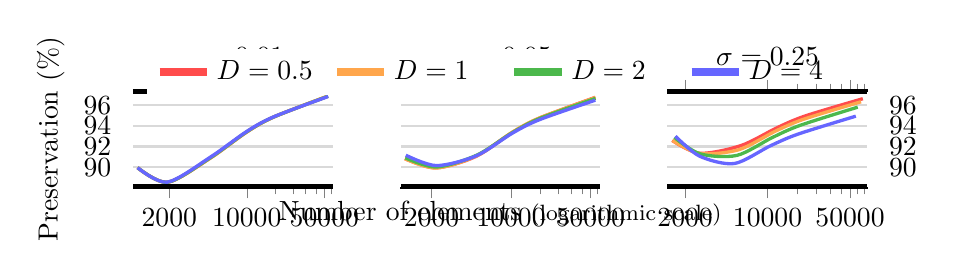
\begin{tikzpicture}
\begin{scope}[shift={(0.0\linewidth,0)}]
\begin{axis}[
 width=0.34\linewidth,height=0.23\linewidth,
 title=\normalsize\mbox{$\sigma=0.01$},
 xmode=log,enlarge x limits=0.025,
 ylabel=Preservation (\%),
 axis y line*=left,
 ymin=88.1171833333,ymax=97.3373908333,
 tick align=outside,
 x axis line style = ultra thick,y axis line style={white},
 xtick={2000,10000,50000},xticklabels={2000,10000,50000},
 minor xtick={18000,26000,34000,42000,58000,66000}, every y tick/.style={white},ymajorgrids,grid style={gray!30,thick}]
\addplot[very thick,mark=none,smooth,color=red!70] table[] {
	1036.16033333 89.9523333333
	1926.05033333 88.5353333333
	4681.20233333 90.8853333333
	9930.996 93.399
	17403.444 94.8616666667
	53726.3493333 96.885
};
\addplot[very thick,mark=none,smooth,color=orange!70] table[] {
	1036.16033333 89.9523333333
	1926.05033333 88.5353333333
	4680.99133333 90.8813333333
	9936.874 93.3996666667
	17410.171 94.863
	53781.8253333 96.8983333333
};
\addplot[very thick,mark=none,smooth,color=green!60!black!70] table[] {
	1036.16033333 89.9523333333
	1926.50133333 88.536
	4686.797 90.912
	9985.02666667 93.4346666667
	17498.657 94.8743333333
	54022.9776667 96.884
};
\addplot[very thick,mark=none,smooth,color=blue!60!] table[] {
	1036.16033333 89.9523333333
	1917.234 88.5486666667
	4693.193 90.976
	9995.812 93.474
	17515.7216667 94.892
	54124.1396667 96.8606666667
};
!\end{axis}
\end{scope}
\begin{scope}[shift={(0.28\linewidth,0)}]
\begin{axis}[
 width=0.34\linewidth,height=0.23\linewidth,
 title=\normalsize\mbox{$\sigma=0.05$},
 xmode=log,enlarge x limits=0.025,
 xlabel=Number of elements \footnotesize(logarithmic scale),x label style={at={(axis description cs:0.5,-0.05)},anchor=north},
 yticklabels={},
 legend style={at={(0.55,1.45)},legend style={text width=4em},legend style={draw=none},anchor=north,legend columns=-1},
 axis y line*=left,
 ymin=88.1171833333,ymax=97.3373908333,
 tick align=outside,
 x axis line style = ultra thick,y axis line style={white},
 xtick={2000,10000,50000},xticklabels={2000,10000,50000},
 minor xtick={18000,26000,34000,42000,58000,66000}, every y tick/.style={white},ymajorgrids,grid style={gray!30,thick}]
\addlegendimage{line width=3pt,mark=none,red!70}
\addlegendentry{$D=0.5$}
\addlegendimage{line width=3pt,mark=none,orange!70}
\addlegendentry{$D=1$}
\addlegendimage{line width=3pt,mark=none,green!60!black!70}
\addlegendentry{$D=2$}
\addlegendimage{line width=3pt,mark=none,blue!60!}
\addlegendentry{$D=4$}
\addplot[very thick,mark=none,smooth,color=red!70] table[] {
	1163.49166667 90.8273333333
	2177.14966667 89.939
	4885.092 91.0303333333
	10297.0083333 93.3843333333
	17952.9826667 94.7843333333
	55333.2983333 96.7773333333
};
\addplot[very thick,mark=none,smooth,color=orange!70] table[] {
	1163.74866667 90.8273333333
	2177.909 89.9183333333
	4930.84733333 91.0886666667
	10320.457 93.416
	18010.387 94.7963333333
	55424.09 96.7586666667
};
\addplot[very thick,mark=none,smooth,color=green!60!black!70] table[] {
	1172.79533333 90.9116666667
	2194.68166667 90.0166666667
	5002.62133333 91.1726666667
	10387.2886667 93.3883333333
	18071.808 94.7496666667
	55454.5933333 96.676
};
\addplot[very thick,mark=none,smooth,color=blue!60!] table[] {
	1184.77533333 91.1646666667
	2197.44466667 90.158
	4945.073 91.1046666667
	10276.6613333 93.305
	17925.9466667 94.6233333333
	55178.0426667 96.4986666667
};
!\end{axis}
\end{scope}
\begin{scope}[shift={(0.56\linewidth,0)}]
\begin{axis}[
 width=0.34\linewidth,height=0.23\linewidth,
 title=\normalsize\mbox{$\sigma=0.25$},
 xmode=log,enlarge x limits=0.025,
 axis y line*=right,
 ymin=88.1171833333,ymax=97.3373908333,
 tick align=outside,
 x axis line style = ultra thick,y axis line style={white},
 xtick={2000,10000,50000},xticklabels={2000,10000,50000},
 minor xtick={18000,26000,34000,42000,58000,66000}, every y tick/.style={white},ymajorgrids,grid style={gray!30,thick}]
\addplot[very thick,mark=none,smooth,color=red!70] table[] {
	1556.41833333 92.5956666667
	2657.71066667 91.3543333333
	5945.90766667 92.0966666667
	12147.856 93.8533333333
	21002.088 94.9846666667
	64168.1893333 96.6466666667
};
\addplot[very thick,mark=none,smooth,color=orange!70] table[] {
	1564.24866667 92.594
	2666.779 91.3296666667
	5704.51666667 91.6983333333
	11594.5613333 93.4843333333
	20113.86 94.6456666667
	61973.142 96.349
};
\addplot[very thick,mark=none,smooth,color=green!60!black!70] table[] {
	1623.46766667 92.8856666667
	2673.40233333 91.2983333333
	5489.90866667 91.1463333333
	11039.2793333 92.896
	19017.0963333 94.0743333333
	58137.1513333 95.827
};
\addplot[very thick,mark=none,smooth,color=blue!60!] table[] {
	1656.86533333 93.0056666667
	2657.24066667 91.0693333333
	5226.841 90.358
	10537.8956667 92.072
	18229.81 93.2213333333
	55998.5563333 94.9526666667
};
!\end{axis}
\end{scope}
\end{tikzpicture}
\end{center}
\caption{Element preservation results using mesh remodelling - Gottingen 459 airfoil}\centering\sffamily\footnotesize
Average of thirty optimisation scenarios\end{figure}

\begin{figure}[!h]
\begin{center}
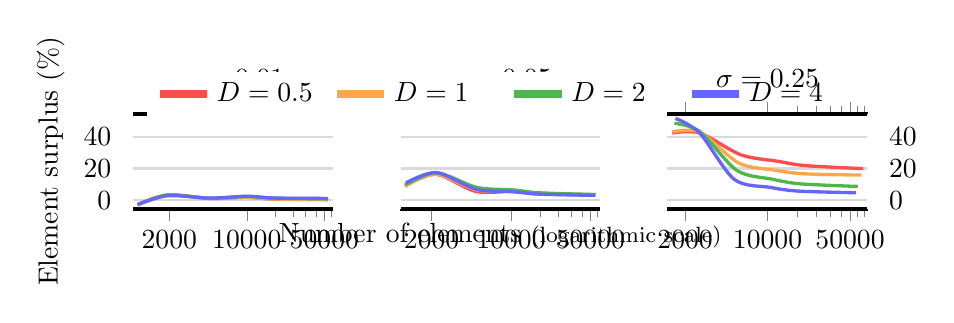
\begin{tikzpicture}
\begin{scope}[shift={(0.0\linewidth,0)}]
\begin{axis}[
 width=0.34\linewidth,height=0.23\linewidth,
 title=\normalsize\mbox{$\sigma=0.01$},
 xmode=log,enlarge x limits=0.025,
 ylabel=Element surplus (\%),
 axis y line*=left,
 ymin=-5.59784247357,ymax=54.4202499872,
 tick align=outside,
 x axis line style = ultra thick,y axis line style={white},
 xtick={2000,10000,50000},xticklabels={2000,10000,50000},
 minor xtick={18000,26000,34000,42000,58000,66000}, every y tick/.style={white},ymajorgrids,grid style={gray!30,thick}]
\addplot[very thick,mark=none,smooth,color=red!70] table[] {
	1036.16033333 -2.87593351843
	1926.05033333 3.21204716406
	4681.20233333 1.01837630643
	9930.996 1.76670319744
	17403.444 0.662798908144
	53726.3493333 0.310376501956
};
\addplot[very thick,mark=none,smooth,color=orange!70] table[] {
	1036.16033333 -2.87593351843
	1926.05033333 3.21204716406
	4680.99133333 1.01382301523
	9936.874 1.82693730502
	17410.171 0.701708370447
	53781.8253333 0.413953583144
};
\addplot[very thick,mark=none,smooth,color=green!60!black!70] table[] {
	1036.16033333 -2.87593351843
	1926.50133333 3.23621508557
	4686.797 1.13910685862
	9985.02666667 2.32037604337
	17498.657 1.21351789643
	54022.9776667 0.864199722164
};
\addplot[very thick,mark=none,smooth,color=blue!60!] table[] {
	1036.16033333 -2.87593351843
	1917.234 2.73960270295
	4693.193 1.27712984692
	9995.812 2.43089746702
	17515.7216667 1.31222118235
	54124.1396667 1.05307535644
};
!\end{axis}
\end{scope}
\begin{scope}[shift={(0.28\linewidth,0)}]
\begin{axis}[
 width=0.34\linewidth,height=0.23\linewidth,
 title=\normalsize\mbox{$\sigma=0.05$},
 xmode=log,enlarge x limits=0.025,
 xlabel=Number of elements \footnotesize(logarithmic scale),x label style={at={(axis description cs:0.5,-0.05)},anchor=north},
 yticklabels={},
 legend style={at={(0.55,1.45)},legend style={text width=4em},legend style={draw=none},anchor=north,legend columns=-1},
 axis y line*=left,
 ymin=-5.59784247357,ymax=54.4202499872,
 tick align=outside,
 x axis line style = ultra thick,y axis line style={white},
 xtick={2000,10000,50000},xticklabels={2000,10000,50000},
 minor xtick={18000,26000,34000,42000,58000,66000}, every y tick/.style={white},ymajorgrids,grid style={gray!30,thick}]
\addlegendimage{line width=3pt,mark=none,red!70}
\addlegendentry{$D=0.5$}
\addlegendimage{line width=3pt,mark=none,orange!70}
\addlegendentry{$D=1$}
\addlegendimage{line width=3pt,mark=none,green!60!black!70}
\addlegendentry{$D=2$}
\addlegendimage{line width=3pt,mark=none,blue!60!}
\addlegendentry{$D=4$}
\addplot[very thick,mark=none,smooth,color=red!70] table[] {
	1163.49166667 8.82242721425
	2177.14966667 16.3361322026
	4885.092 5.46439188348
	10297.0083333 5.51095957445
	17952.9826667 3.89163763232
	55333.2983333 3.28924690375
};
\addplot[very thick,mark=none,smooth,color=orange!70] table[] {
	1163.74866667 8.84646465654
	2177.909 16.376707228
	4930.84733333 6.45220509261
	10320.457 5.75123240328
	18010.387 4.22382924125
	55424.09 3.45872537616
};
\addplot[very thick,mark=none,smooth,color=green!60!black!70] table[] {
	1172.79533333 9.69260756677
	2194.68166667 17.2729557481
	5002.62133333 8.00173604577
	10387.2886667 6.43604036417
	18071.808 4.57926479162
	55454.5933333 3.5156651651
};
\addplot[very thick,mark=none,smooth,color=blue!60!] table[] {
	1184.77533333 10.813107795
	2197.44466667 17.4205968305
	4945.073 6.75932341999
	10276.6613333 5.30246877548
	17925.9466667 3.73518372339
	55178.0426667 2.99943513813
};
!\end{axis}
\end{scope}
\begin{scope}[shift={(0.56\linewidth,0)}]
\begin{axis}[
 width=0.34\linewidth,height=0.23\linewidth,
 title=\normalsize\mbox{$\sigma=0.25$},
 xmode=log,enlarge x limits=0.025,
 axis y line*=right,
 ymin=-5.59784247357,ymax=54.4202499872,
 tick align=outside,
 x axis line style = ultra thick,y axis line style={white},
 xtick={2000,10000,50000},xticklabels={2000,10000,50000},
 minor xtick={18000,26000,34000,42000,58000,66000}, every y tick/.style={white},ymajorgrids,grid style={gray!30,thick}]
\addplot[very thick,mark=none,smooth,color=red!70] table[] {
	1556.41833333 42.3738266006
	2657.71066667 42.3641376158
	5945.90766667 28.5837788446
	12147.856 24.5255422874
	21002.088 21.7544745104
	64168.1893333 19.8888272685
};
\addplot[very thick,mark=none,smooth,color=orange!70] table[] {
	1564.24866667 43.0901086544
	2666.779 42.8498960811
	5704.51666667 23.3635553397
	11594.5613333 18.8538156542
	20113.86 16.6051896685
	61973.142 15.7877040589
};
\addplot[very thick,mark=none,smooth,color=green!60!black!70] table[] {
	1623.46766667 48.5071841648
	2673.40233333 43.204684565
	5489.90866667 18.7225300906
	11039.2793333 13.1617172154
	19017.0963333 10.2469702431
	58137.1513333 8.62071949513
};
\addplot[very thick,mark=none,smooth,color=blue!60!] table[] {
	1656.86533333 51.5622455843
	2657.24066667 42.3389613822
	5226.841 13.0335358162
	10537.8956667 8.02212114302
	18229.81 5.68287005434
	55998.5563333 4.62506917032
};
!\end{axis}
\end{scope}
\end{tikzpicture}
\end{center}
\caption{Element surplus results on meshes from mesh remodelling - Gottingen 459 airfoil}\centering\sffamily\footnotesize
Average of thirty optimisation scenarios\end{figure}

\begin{figure}[!h]
\begin{center}
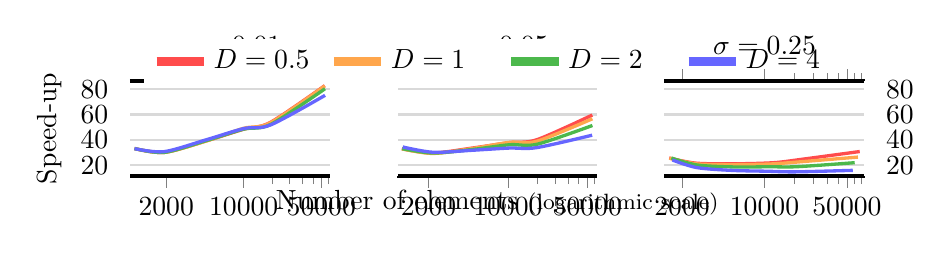
\begin{tikzpicture}
\begin{scope}[shift={(0.0\linewidth,0)}]
\begin{axis}[
 width=0.34\linewidth,height=0.23\linewidth,
 title=\normalsize\mbox{$\sigma=0.01$},
 xmode=log,enlarge x limits=0.025,
 ylabel=Speed-up,
 axis y line*=left,
 ymin=11.306562195,ymax=86.3569465468,
 tick align=outside,
 x axis line style = ultra thick,y axis line style={white},
 xtick={2000,10000,50000},xticklabels={2000,10000,50000},
 minor xtick={18000,26000,34000,42000,58000,66000}, every y tick/.style={white},ymajorgrids,grid style={gray!30,thick}]
\addplot[very thick,mark=none,smooth,color=red!70] table[] {
	1036.16033333 33.1281540505
	1926.05033333 30.0858381503
	4681.20233333 39.365481542
	9930.996 48.3273577553
	17403.444 53.7921724053
	53726.3493333 82.7831187206
};
\addplot[very thick,mark=none,smooth,color=orange!70] table[] {
	1036.16033333 33.1061712011
	1926.05033333 30.0771453337
	4680.99133333 39.3012375901
	9936.874 49.069325736
	17410.171 53.4374231015
	53781.8253333 82.5259502598
};
\addplot[very thick,mark=none,smooth,color=green!60!black!70] table[] {
	1036.16033333 33.1281540505
	1926.50133333 30.0858381503
	4686.797 39.591998904
	9985.02666667 48.4330573348
	17498.657 52.1465277111
	54022.9776667 80.3274190185
};
\addplot[very thick,mark=none,smooth,color=blue!60!] table[] {
	1036.16033333 33.0622929092
	1917.234 30.6618556701
	4693.193 40.2874668897
	9995.812 48.8913420596
	17515.7216667 51.7982539834
	54124.1396667 75.1285797874
};
!\end{axis}
\end{scope}
\begin{scope}[shift={(0.28\linewidth,0)}]
\begin{axis}[
 width=0.34\linewidth,height=0.23\linewidth,
 title=\normalsize\mbox{$\sigma=0.05$},
 xmode=log,enlarge x limits=0.025,
 xlabel=Number of elements \footnotesize(logarithmic scale),x label style={at={(axis description cs:0.5,-0.05)},anchor=north},
 yticklabels={},
 legend style={at={(0.55,1.45)},legend style={text width=4em},legend style={draw=none},anchor=north,legend columns=-1},
 axis y line*=left,
 ymin=11.306562195,ymax=86.3569465468,
 tick align=outside,
 x axis line style = ultra thick,y axis line style={white},
 xtick={2000,10000,50000},xticklabels={2000,10000,50000},
 minor xtick={18000,26000,34000,42000,58000,66000}, every y tick/.style={white},ymajorgrids,grid style={gray!30,thick}]
\addlegendimage{line width=3pt,mark=none,red!70}
\addlegendentry{$D=0.5$}
\addlegendimage{line width=3pt,mark=none,orange!70}
\addlegendentry{$D=1$}
\addlegendimage{line width=3pt,mark=none,green!60!black!70}
\addlegendentry{$D=2$}
\addlegendimage{line width=3pt,mark=none,blue!60!}
\addlegendentry{$D=4$}
\addplot[very thick,mark=none,smooth,color=red!70] table[] {
	1163.49166667 32.9511873351
	2177.14966667 29.5927293383
	4885.092 33.5371900826
	10297.0083333 37.7851198915
	17952.9826667 40.059654573
	55333.2983333 59.584514947
};
\addplot[very thick,mark=none,smooth,color=orange!70] table[] {
	1163.74866667 32.8861092824
	2177.909 29.2356902357
	4930.84733333 33.2086214846
	10320.457 38.0124023316
	18010.387 38.939245785
	55424.09 56.6006520167
};
\addplot[very thick,mark=none,smooth,color=green!60!black!70] table[] {
	1172.79533333 33.0165234633
	2194.68166667 29.5675368899
	5002.62133333 32.5042870036
	10387.2886667 36.1474230452
	18071.808 36.5270452553
	55454.5933333 51.3095314809
};
\addplot[very thick,mark=none,smooth,color=blue!60!] table[] {
	1184.77533333 34.356258597
	2197.44466667 30.1667631731
	4945.073 31.7870697264
	10276.6613333 33.4838040094
	17925.9466667 33.8364675747
	55178.0426667 43.6504442344
};
!\end{axis}
\end{scope}
\begin{scope}[shift={(0.56\linewidth,0)}]
\begin{axis}[
 width=0.34\linewidth,height=0.23\linewidth,
 title=\normalsize\mbox{$\sigma=0.25$},
 xmode=log,enlarge x limits=0.025,
 axis y line*=right,
 ymin=11.306562195,ymax=86.3569465468,
 tick align=outside,
 x axis line style = ultra thick,y axis line style={white},
 xtick={2000,10000,50000},xticklabels={2000,10000,50000},
 minor xtick={18000,26000,34000,42000,58000,66000}, every y tick/.style={white},ymajorgrids,grid style={gray!30,thick}]
\addplot[very thick,mark=none,smooth,color=red!70] table[] {
	1556.41833333 25.6236068896
	2657.71066667 21.5349080268
	5945.90766667 21.0973834959
	12147.856 21.9918791743
	21002.088 24.6988434885
	64168.1893333 30.7508832614
};
\addplot[very thick,mark=none,smooth,color=orange!70] table[] {
	1564.24866667 25.533064109
	2666.779 21.0165238678
	5704.51666667 20.382619101
	11594.5613333 20.9936605687
	20113.86 22.6470800748
	61973.142 26.3740512649
};
\addplot[very thick,mark=none,smooth,color=green!60!black!70] table[] {
	1623.46766667 25.6236068896
	2673.40233333 20.1374120407
	5489.90866667 18.5853791598
	11039.2793333 18.7277427694
	19017.0963333 18.7887833001
	58137.1513333 21.9512838373
};
\addplot[very thick,mark=none,smooth,color=blue!60!] table[] {
	1656.86533333 24.0632730733
	2657.24066667 18.0964342175
	5226.841 15.8718770019
	10537.8956667 15.1944102147
	18229.81 14.7102077438
	55998.5563333 15.8957546284
};
!\end{axis}
\end{scope}
\end{tikzpicture}
\end{center}
\caption{Speed-up results by mesh remodelling - Gottingen 459 airfoil}\centering\sffamily\footnotesize
Average of thirty optimisation scenarios\end{figure}

\pagebreak
\subsubsection{NACA 2412}
\vspace*{\fill} \begin{table}[!hp]
\begin{center}
\begin{tabular}{c|cc?c|c?c?c|c|c||c|c}
\multirow{2}{*}{\textbf{\large $\boldsymbol{\sigma}$}} & \multirow{2}{*}{\textbf{\large $\boldsymbol{I}$}} & \multirow{2}{*}{\textbf{\large $\boldsymbol{G}$}} & \multicolumn{2}{c?}{\textbf{\large Generation}} & \multirow{2}{*}{\textbf{\large $\boldsymbol{D}$}} & \multicolumn{5}{c}{\textbf{{\large Remodelling} }} \\\cline{4-5}\cline{7-11}
 & & & \textbf{\# Tri.} & \textbf{Time} & &\textbf{\# Tri.} & \textbf{Time} & \textbf{Preserv.} & \textbf{+ Tri.} & \textbf{Sp.-up} \\\toprule
\multirow{24}[13]{*}{.01} & \multirow{4}{*}{50} & \multirow{4}{*}{1} & \multirow{4}{*}{1048} & \multirow{4}{*}{1.64 ms} & .5 & 1115 & 0.05 ms & 90.49 \% & 6.45 \% & 32.23 \\\cline{6-11}
 & & & &  & 1 & 1115 & 0.05 ms & 90.49 \% & 6.45 \% & 32.23 \\\cline{6-11}
 & & & &  & 2 & 1115 & 0.05 ms & 90.52 \% & 6.43 \% & 32.31 \\\cline{6-11}
 & & & &  & 4 & 1114 & 0.05 ms & 90.58 \% & 6.37 \% & 33.25 \\\cmidrule[1.5pt]{2-11}
 & \multirow{4}{*}{100} & \multirow{4}{*}{2} & \multirow{4}{*}{1823} & \multirow{4}{*}{3.39 ms} & .5 & 2154 & 0.12 ms & 89.75 \% & 18.16 \% & 28.42 \\\cline{6-11}
 & & & &  & 1 & 2153 & 0.12 ms & 89.77 \% & 18.14 \% & 28.68 \\\cline{6-11}
 & & & &  & 2 & 2147 & 0.12 ms & 89.76 \% & 17.80 \% & 28.75 \\\cline{6-11}
 & & & &  & 4 & 2130 & 0.11 ms & 89.87 \% & 16.86 \% & 29.74 \\\cmidrule[1.5pt]{2-11}
 & \multirow{4}{*}{200} & \multirow{4}{*}{4} & \multirow{4}{*}{4618} & \multirow{4}{*}{9.49 ms} & .5 & 4981 & 0.29 ms & 91.19 \% & 7.86 \% & 32.36 \\\cline{6-11}
 & & & &  & 1 & 4967 & 0.29 ms & 91.17 \% & 7.54 \% & 32.64 \\\cline{6-11}
 & & & &  & 2 & 4982 & 0.30 ms & 91.18 \% & 7.88 \% & 32.02 \\\cline{6-11}
 & & & &  & 4 & 4907 & 0.29 ms & 91.12 \% & 6.26 \% & 32.18 \\\cmidrule[1.5pt]{2-11}
 & \multirow{4}{*}{300} & \multirow{4}{*}{6} & \multirow{4}{*}{9781} & \multirow{4}{*}{20.52 ms} & .5 & 10377 & 0.55 ms & 93.47 \% & 6.08 \% & 37.12 \\\cline{6-11}
 & & & &  & 1 & 10369 & 0.56 ms & 93.48 \% & 6.01 \% & 36.85 \\\cline{6-11}
 & & & &  & 2 & 10390 & 0.58 ms & 93.46 \% & 6.23 \% & 35.13 \\\cline{6-11}
 & & & &  & 4 & 10286 & 0.59 ms & 93.37 \% & 5.16 \% & 34.81 \\\cmidrule[1.5pt]{2-11}
 & \multirow{4}{*}{400} & \multirow{4}{*}{8} & \multirow{4}{*}{17288} & \multirow{4}{*}{35.91 ms} & .5 & 18148 & 0.96 ms & 94.86 \% & 4.97 \% & 37.22 \\\cline{6-11}
 & & & &  & 1 & 18134 & 0.98 ms & 94.86 \% & 4.89 \% & 36.78 \\\cline{6-11}
 & & & &  & 2 & 18107 & 1.02 ms & 94.80 \% & 4.74 \% & 35.30 \\\cline{6-11}
 & & & &  & 4 & 17957 & 1.07 ms & 94.68 \% & 3.87 \% & 33.61 \\\cmidrule[1.5pt]{2-11}
 & \multirow{4}{*}{700} & \multirow{4}{*}{14} & \multirow{4}{*}{53632} & \multirow{4}{*}{153.47 ms} & .5 & 55929 & 2.85 ms & 96.84 \% & 4.28 \% & 53.91 \\\cline{6-11}
 & & & &  & 1 & 55791 & 2.97 ms & 96.81 \% & 4.03 \% & 51.60 \\\cline{6-11}
 & & & &  & 2 & 55631 & 3.26 ms & 96.71 \% & 3.73 \% & 47.03 \\\cline{6-11}
 & & & &  & 4 & 55294 & 3.75 ms & 96.53 \% & 3.10 \% & 40.91\\\bottomrule
\end{tabular}\end{center}
\caption{Full results of mesh remodelling for $\sigma=0.01$ - NACA 2412 airfoil}\centering\sffamily\footnotesize
Average of thirty optimisation scenarios\end{table}
 \vspace*{\fill}
\begin{table}[!hp]
\begin{center}
\begin{tabular}{c|cc?c|c?c?c|c|c||c|c}
\multirow{2}{*}{\textbf{\large $\boldsymbol{\sigma}$}} & \multirow{2}{*}{\textbf{\large $\boldsymbol{I}$}} & \multirow{2}{*}{\textbf{\large $\boldsymbol{G}$}} & \multicolumn{2}{c?}{\textbf{\large Generation}} & \multirow{2}{*}{\textbf{\large $\boldsymbol{D}$}} & \multicolumn{5}{c}{\textbf{{\large Remodelling} }} \\\cline{4-5}\cline{7-11}
 & & & \textbf{\# Tri.} & \textbf{Time} & &\textbf{\# Tri.} & \textbf{Time} & \textbf{Preserv.} & \textbf{+ Tri.} & \textbf{Sp.-up} \\\toprule
\multirow{24}[13]{*}{.05} & \multirow{4}{*}{50} & \multirow{4}{*}{1} & \multirow{4}{*}{1062} & \multirow{4}{*}{1.65 ms} & .5 & 1295 & 0.05 ms & 91.44 \% & 21.95 \% & 31.17 \\\cline{6-11}
 & & & &  & 1 & 1303 & 0.05 ms & 91.48 \% & 22.73 \% & 31.25 \\\cline{6-11}
 & & & &  & 2 & 1298 & 0.05 ms & 91.52 \% & 22.18 \% & 31.21 \\\cline{6-11}
 & & & &  & 4 & 1299 & 0.05 ms & 91.62 \% & 22.29 \% & 32.14 \\\cmidrule[1.5pt]{2-11}
 & \multirow{4}{*}{100} & \multirow{4}{*}{2} & \multirow{4}{*}{1818} & \multirow{4}{*}{3.37 ms} & .5 & 2320 & 0.13 ms & 90.38 \% & 27.60 \% & 25.82 \\\cline{6-11}
 & & & &  & 1 & 2326 & 0.13 ms & 90.42 \% & 27.94 \% & 25.94 \\\cline{6-11}
 & & & &  & 2 & 2346 & 0.13 ms & 90.51 \% & 29.07 \% & 25.98 \\\cline{6-11}
 & & & &  & 4 & 2311 & 0.13 ms & 90.49 \% & 27.14 \% & 26.42 \\\cmidrule[1.5pt]{2-11}
 & \multirow{4}{*}{200} & \multirow{4}{*}{4} & \multirow{4}{*}{4617} & \multirow{4}{*}{9.38 ms} & .5 & 5139 & 0.33 ms & 91.28 \% & 11.29 \% & 28.84 \\\cline{6-11}
 & & & &  & 1 & 5118 & 0.32 ms & 91.27 \% & 10.84 \% & 28.89 \\\cline{6-11}
 & & & &  & 2 & 5136 & 0.34 ms & 91.24 \% & 11.24 \% & 27.89 \\\cline{6-11}
 & & & &  & 4 & 5030 & 0.35 ms & 91.06 \% & 8.94 \% & 26.97 \\\cmidrule[1.5pt]{2-11}
 & \multirow{4}{*}{300} & \multirow{4}{*}{6} & \multirow{4}{*}{9783} & \multirow{4}{*}{19.84 ms} & .5 & 10653 & 0.63 ms & 93.48 \% & 8.89 \% & 31.27 \\\cline{6-11}
 & & & &  & 1 & 10642 & 0.64 ms & 93.46 \% & 8.78 \% & 30.86 \\\cline{6-11}
 & & & &  & 2 & 10592 & 0.70 ms & 93.36 \% & 8.27 \% & 28.38 \\\cline{6-11}
 & & & &  & 4 & 10376 & 0.73 ms & 93.12 \% & 6.07 \% & 27.23 \\\cmidrule[1.5pt]{2-11}
 & \multirow{4}{*}{400} & \multirow{4}{*}{8} & \multirow{4}{*}{17288} & \multirow{4}{*}{35.80 ms} & .5 & 18583 & 1.11 ms & 94.83 \% & 7.49 \% & 32.13 \\\cline{6-11}
 & & & &  & 1 & 18521 & 1.13 ms & 94.79 \% & 7.13 \% & 31.60 \\\cline{6-11}
 & & & &  & 2 & 18418 & 1.22 ms & 94.66 \% & 6.54 \% & 29.31 \\\cline{6-11}
 & & & &  & 4 & 18060 & 1.34 ms & 94.40 \% & 4.46 \% & 26.72 \\\cmidrule[1.5pt]{2-11}
 & \multirow{4}{*}{700} & \multirow{4}{*}{14} & \multirow{4}{*}{53646} & \multirow{4}{*}{153.45 ms} & .5 & 57211 & 3.39 ms & 96.75 \% & 6.65 \% & 45.32 \\\cline{6-11}
 & & & &  & 1 & 56982 & 3.59 ms & 96.69 \% & 6.22 \% & 42.78 \\\cline{6-11}
 & & & &  & 2 & 56504 & 4.08 ms & 96.54 \% & 5.33 \% & 37.61 \\\cline{6-11}
 & & & &  & 4 & 55566 & 4.90 ms & 96.23 \% & 3.58 \% & 31.33\\\bottomrule
\end{tabular}\end{center}
\caption{Full results of mesh remodelling for $\sigma=0.05$ - NACA 2412 airfoil}\centering\sffamily\footnotesize
Average of thirty optimisation scenarios\end{table}

\begin{table}[!hp]
\begin{center}
\begin{tabular}{c|cc?c|c?c?c|c|c||c|c}
\multirow{2}{*}{\textbf{\large $\boldsymbol{\sigma}$}} & \multirow{2}{*}{\textbf{\large $\boldsymbol{I}$}} & \multirow{2}{*}{\textbf{\large $\boldsymbol{G}$}} & \multicolumn{2}{c?}{\textbf{\large Generation}} & \multirow{2}{*}{\textbf{\large $\boldsymbol{D}$}} & \multicolumn{5}{c}{\textbf{{\large Remodelling} }} \\\cline{4-5}\cline{7-11}
 & & & \textbf{\# Tri.} & \textbf{Time} & &\textbf{\# Tri.} & \textbf{Time} & \textbf{Preserv.} & \textbf{+ Tri.} & \textbf{Sp.-up} \\\toprule
\multirow{24}[13]{*}{.25} & \multirow{4}{*}{50} & \multirow{4}{*}{1} & \multirow{4}{*}{1084} & \multirow{4}{*}{1.67 ms} & .5 & 1570 & 0.07 ms & 92.66 \% & 44.88 \% & 25.39 \\\cline{6-11}
 & & & &  & 1 & 1592 & 0.07 ms & 92.72 \% & 46.85 \% & 25.20 \\\cline{6-11}
 & & & &  & 2 & 1610 & 0.07 ms & 92.78 \% & 48.57 \% & 24.96 \\\cline{6-11}
 & & & &  & 4 & 1664 & 0.07 ms & 93.04 \% & 53.51 \% & 23.36 \\\cmidrule[1.5pt]{2-11}
 & \multirow{4}{*}{100} & \multirow{4}{*}{2} & \multirow{4}{*}{1822} & \multirow{4}{*}{3.34 ms} & .5 & 2669 & 0.16 ms & 91.37 \% & 46.44 \% & 20.34 \\\cline{6-11}
 & & & &  & 1 & 2668 & 0.17 ms & 91.29 \% & 46.42 \% & 19.96 \\\cline{6-11}
 & & & &  & 2 & 2668 & 0.17 ms & 91.25 \% & 46.39 \% & 19.17 \\\cline{6-11}
 & & & &  & 4 & 2645 & 0.19 ms & 90.99 \% & 45.11 \% & 17.19 \\\cmidrule[1.5pt]{2-11}
 & \multirow{4}{*}{200} & \multirow{4}{*}{4} & \multirow{4}{*}{4610} & \multirow{4}{*}{8.98 ms} & .5 & 5943 & 0.44 ms & 92.09 \% & 28.91 \% & 20.40 \\\cline{6-11}
 & & & &  & 1 & 5717 & 0.46 ms & 91.68 \% & 24.01 \% & 19.67 \\\cline{6-11}
 & & & &  & 2 & 5463 & 0.51 ms & 91.06 \% & 18.50 \% & 17.76 \\\cline{6-11}
 & & & &  & 4 & 5240 & 0.60 ms & 90.29 \% & 13.67 \% & 15.07 \\\cmidrule[1.5pt]{2-11}
 & \multirow{4}{*}{300} & \multirow{4}{*}{6} & \multirow{4}{*}{9778} & \multirow{4}{*}{19.19 ms} & .5 & 12118 & 0.91 ms & 93.84 \% & 23.94 \% & 21.20 \\\cline{6-11}
 & & & &  & 1 & 11591 & 0.95 ms & 93.45 \% & 18.55 \% & 20.17 \\\cline{6-11}
 & & & &  & 2 & 10997 & 1.08 ms & 92.86 \% & 12.47 \% & 17.79 \\\cline{6-11}
 & & & &  & 4 & 10558 & 1.33 ms & 91.99 \% & 7.99 \% & 14.46 \\\cmidrule[1.5pt]{2-11}
 & \multirow{4}{*}{400} & \multirow{4}{*}{8} & \multirow{4}{*}{17273} & \multirow{4}{*}{35.35 ms} & .5 & 20974 & 1.51 ms & 94.97 \% & 21.43 \% & 23.36 \\\cline{6-11}
 & & & &  & 1 & 20113 & 1.69 ms & 94.61 \% & 16.45 \% & 20.90 \\\cline{6-11}
 & & & &  & 2 & 18937 & 1.99 ms & 94.02 \% & 9.64 \% & 17.81 \\\cline{6-11}
 & & & &  & 4 & 18201 & 2.55 ms & 93.12 \% & 5.37 \% & 13.86 \\\cmidrule[1.5pt]{2-11}
 & \multirow{4}{*}{700} & \multirow{4}{*}{14} & \multirow{4}{*}{53607} & \multirow{4}{*}{151.91 ms} & .5 & 64172 & 5.29 ms & 96.62 \% & 19.71 \% & 28.70 \\\cline{6-11}
 & & & &  & 1 & 61833 & 6.15 ms & 96.32 \% & 15.34 \% & 24.69 \\\cline{6-11}
 & & & &  & 2 & 57864 & 7.40 ms & 95.76 \% & 7.94 \% & 20.54 \\\cline{6-11}
 & & & &  & 4 & 55940 & 10.16 ms & 94.86 \% & 4.35 \% & 14.95\\\bottomrule
\end{tabular}\end{center}
\caption{Full results of mesh remodelling for $\sigma=0.25$ - NACA 2412 airfoil}\centering\sffamily\footnotesize
Average of thirty optimisation scenarios\end{table}
 \newpage
\begin{figure}[!h]
\begin{center}
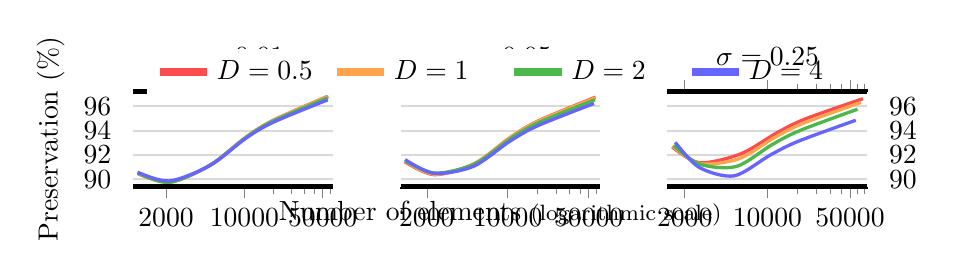
\begin{tikzpicture}
\begin{scope}[shift={(0.0\linewidth,0)}]
\begin{axis}[
 width=0.34\linewidth,height=0.23\linewidth,
 title=\normalsize\mbox{$\sigma=0.01$},
 xmode=log,enlarge x limits=0.025,
 ylabel=Preservation (\%),
 axis y line*=left,
 ymin=89.4003666667,ymax=97.2126816667,
 tick align=outside,
 x axis line style = ultra thick,y axis line style={white},
 xtick={2000,10000,50000},xticklabels={2000,10000,50000},
 minor xtick={18000,26000,34000,42000,58000,66000}, every y tick/.style={white},ymajorgrids,grid style={gray!30,thick}]
\addplot[very thick,mark=none,smooth,color=red!70] table[] {
	1115.258 90.4886666667
	2153.71966667 89.7546666667
	4981.13166667 91.187
	10376.6173333 93.4746666667
	18148.2636667 94.8566666667
	55929.1186667 96.8406666667
};
\addplot[very thick,mark=none,smooth,color=orange!70] table[] {
	1115.258 90.4886666667
	2153.35533333 89.765
	4966.71566667 91.173
	10369.0493333 93.477
	18133.7363333 94.8606666667
	55791.018 96.809
};
\addplot[very thick,mark=none,smooth,color=green!60!black!70] table[] {
	1115.04066667 90.516
	2147.23566667 89.7583333333
	4982.24466667 91.1813333333
	10390.4563333 93.456
	18107.314 94.7993333333
	55630.722 96.7063333333
};
\addplot[very thick,mark=none,smooth,color=blue!60!] table[] {
	1114.39433333 90.584
	2129.97033333 89.867
	4907.451 91.1223333333
	10285.6763333 93.369
	17956.7793333 94.6793333333
	55294.329 96.532
};
!\end{axis}
\end{scope}
\begin{scope}[shift={(0.28\linewidth,0)}]
\begin{axis}[
 width=0.34\linewidth,height=0.23\linewidth,
 title=\normalsize\mbox{$\sigma=0.05$},
 xmode=log,enlarge x limits=0.025,
 xlabel=Number of elements \footnotesize(logarithmic scale),x label style={at={(axis description cs:0.5,-0.05)},anchor=north},
 yticklabels={},
 legend style={at={(0.55,1.45)},legend style={text width=4em},legend style={draw=none},anchor=north,legend columns=-1},
 axis y line*=left,
 ymin=89.4003666667,ymax=97.2126816667,
 tick align=outside,
 x axis line style = ultra thick,y axis line style={white},
 xtick={2000,10000,50000},xticklabels={2000,10000,50000},
 minor xtick={18000,26000,34000,42000,58000,66000}, every y tick/.style={white},ymajorgrids,grid style={gray!30,thick}]
\addlegendimage{line width=3pt,mark=none,red!70}
\addlegendentry{$D=0.5$}
\addlegendimage{line width=3pt,mark=none,orange!70}
\addlegendentry{$D=1$}
\addlegendimage{line width=3pt,mark=none,green!60!black!70}
\addlegendentry{$D=2$}
\addlegendimage{line width=3pt,mark=none,blue!60!}
\addlegendentry{$D=4$}
\addplot[very thick,mark=none,smooth,color=red!70] table[] {
	1295.23666667 91.4383333333
	2319.814 90.383
	5138.91666667 91.278
	10652.52 93.4846666667
	18583.1506667 94.827
	57210.9673333 96.7516666667
};
\addplot[very thick,mark=none,smooth,color=orange!70] table[] {
	1303.43733333 91.4796666667
	2325.93266667 90.4166666667
	5118.09633333 91.2683333333
	10641.6626667 93.463
	18521.3283333 94.7893333333
	56982.0486667 96.688
};
\addplot[very thick,mark=none,smooth,color=green!60!black!70] table[] {
	1297.58333333 91.5216666667
	2346.43866667 90.5123333333
	5136.495 91.243
	10591.5073333 93.3576666667
	18417.8746667 94.661
	56504.481 96.5383333333
};
\addplot[very thick,mark=none,smooth,color=blue!60!] table[] {
	1298.755 91.6193333333
	2311.45166667 90.4946666667
	5030.275 91.057
	10376.187 93.117
	18059.9306667 94.3973333333
	55565.6503333 96.232
};
!\end{axis}
\end{scope}
\begin{scope}[shift={(0.56\linewidth,0)}]
\begin{axis}[
 width=0.34\linewidth,height=0.23\linewidth,
 title=\normalsize\mbox{$\sigma=0.25$},
 xmode=log,enlarge x limits=0.025,
 axis y line*=right,
 ymin=89.4003666667,ymax=97.2126816667,
 tick align=outside,
 x axis line style = ultra thick,y axis line style={white},
 xtick={2000,10000,50000},xticklabels={2000,10000,50000},
 minor xtick={18000,26000,34000,42000,58000,66000}, every y tick/.style={white},ymajorgrids,grid style={gray!30,thick}]
\addplot[very thick,mark=none,smooth,color=red!70] table[] {
	1570.24733333 92.6633333333
	2668.77166667 91.3656666667
	5942.79166667 92.089
	12118.3263333 93.8403333333
	20973.5136667 94.9653333333
	64172.085 96.6246666667
};
\addplot[very thick,mark=none,smooth,color=orange!70] table[] {
	1591.61966667 92.7176666667
	2668.32066667 91.2916666667
	5716.86733333 91.683
	11591.0006667 93.4543333333
	20113.2883333 94.611
	61832.7416667 96.32
};
\addplot[very thick,mark=none,smooth,color=green!60!black!70] table[] {
	1610.32533333 92.78
	2667.697 91.254
	5462.71833333 91.0553333333
	10996.7966667 92.86
	18937.3753333 94.0186666667
	57864.3813333 95.763
};
\addplot[very thick,mark=none,smooth,color=blue!60!] table[] {
	1663.819 93.043
	2644.519 90.9866666667
	5240.154 90.2863333333
	10558.453 91.991
	18200.8403333 93.1233333333
	55939.5143333 94.8556666667
};
!\end{axis}
\end{scope}
\end{tikzpicture}
\end{center}
\caption{Element preservation results using mesh remodelling - NACA 2412 airfoil}\centering\sffamily\footnotesize
Average of thirty optimisation scenarios\end{figure}

\begin{figure}[!h]
\begin{center}
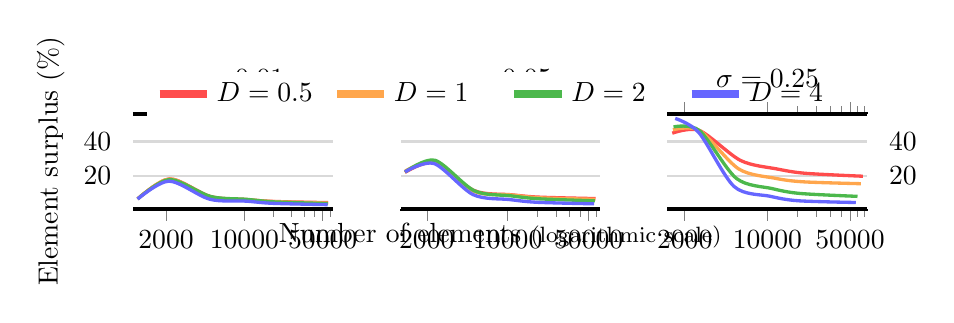
\begin{tikzpicture}
\begin{scope}[shift={(0.0\linewidth,0)}]
\begin{axis}[
 width=0.34\linewidth,height=0.23\linewidth,
 title=\normalsize\mbox{$\sigma=0.01$},
 xmode=log,enlarge x limits=0.025,
 ylabel=Element surplus (\%),
 axis y line*=left,
 ymin=0.579218231148,ymax=56.1570690355,
 tick align=outside,
 x axis line style = ultra thick,y axis line style={white},
 xtick={2000,10000,50000},xticklabels={2000,10000,50000},
 minor xtick={18000,26000,34000,42000,58000,66000}, every y tick/.style={white},ymajorgrids,grid style={gray!30,thick}]
\addplot[very thick,mark=none,smooth,color=red!70] table[] {
	1115.258 6.45076001623
	2153.71966667 18.1595471241
	4981.13166667 7.85570510779
	10376.6173333 6.08478719539
	18148.2636667 4.97346703252
	55929.1186667 4.2833609587
};
\addplot[very thick,mark=none,smooth,color=orange!70] table[] {
	1115.258 6.45076001623
	2153.35533333 18.1395587002
	4966.71566667 7.54355759817
	10369.0493333 6.0074161559
	18133.7363333 4.88943780665
	55791.018 4.02586357605
};
\addplot[very thick,mark=none,smooth,color=green!60!black!70] table[] {
	1115.04066667 6.43001566962
	2147.23566667 17.8038153567
	4982.24466667 7.8798047317
	10390.4563333 6.22626946489
	18107.314 4.73660533804
	55630.722 3.72698159781
};
\addplot[very thick,mark=none,smooth,color=blue!60!] table[] {
	1114.39433333 6.36832350999
	2129.97033333 16.8565871732
	4907.451 6.2603085618
	10285.6763333 5.15505679073
	17956.7793333 3.86588039384
	55294.329 3.09975568259
};
!\end{axis}
\end{scope}
\begin{scope}[shift={(0.28\linewidth,0)}]
\begin{axis}[
 width=0.34\linewidth,height=0.23\linewidth,
 title=\normalsize\mbox{$\sigma=0.05$},
 xmode=log,enlarge x limits=0.025,
 xlabel=Number of elements \footnotesize(logarithmic scale),x label style={at={(axis description cs:0.5,-0.05)},anchor=north},
 yticklabels={},
 legend style={at={(0.55,1.45)},legend style={text width=4em},legend style={draw=none},anchor=north,legend columns=-1},
 axis y line*=left,
 ymin=0.579218231148,ymax=56.1570690355,
 tick align=outside,
 x axis line style = ultra thick,y axis line style={white},
 xtick={2000,10000,50000},xticklabels={2000,10000,50000},
 minor xtick={18000,26000,34000,42000,58000,66000}, every y tick/.style={white},ymajorgrids,grid style={gray!30,thick}]
\addlegendimage{line width=3pt,mark=none,red!70}
\addlegendentry{$D=0.5$}
\addlegendimage{line width=3pt,mark=none,orange!70}
\addlegendentry{$D=1$}
\addlegendimage{line width=3pt,mark=none,green!60!black!70}
\addlegendentry{$D=2$}
\addlegendimage{line width=3pt,mark=none,blue!60!}
\addlegendentry{$D=4$}
\addplot[very thick,mark=none,smooth,color=red!70] table[] {
	1295.23666667 21.9546719093
	2319.814 27.6019219564
	5138.91666667 11.2929085986
	10652.52 8.89356238619
	18583.1506667 7.49118337079
	57210.9673333 6.64526523409
};
\addplot[very thick,mark=none,smooth,color=orange!70] table[] {
	1303.43733333 22.726816212
	2325.93266667 27.9384806746
	5118.09633333 10.8420051096
	10641.6626667 8.78257515456
	18521.3283333 7.13358223587
	56982.0486667 6.21854474567
};
\addplot[very thick,mark=none,smooth,color=green!60!black!70] table[] {
	1297.58333333 22.1756253233
	2346.43866667 29.0664180919
	5136.495 11.2404628509
	10591.5073333 8.26987084428
	18417.8746667 6.53517148984
	56504.481 5.32832504037
};
\addplot[very thick,mark=none,smooth,color=blue!60!] table[] {
	1298.755 22.2859451031
	2311.45166667 27.1419498184
	5030.275 8.9400689122
	10376.187 6.06879559159
	18059.9306667 4.46470320216
	55565.6503333 3.57827867473
};
!\end{axis}
\end{scope}
\begin{scope}[shift={(0.56\linewidth,0)}]
\begin{axis}[
 width=0.34\linewidth,height=0.23\linewidth,
 title=\normalsize\mbox{$\sigma=0.25$},
 xmode=log,enlarge x limits=0.025,
 axis y line*=right,
 ymin=0.579218231148,ymax=56.1570690355,
 tick align=outside,
 x axis line style = ultra thick,y axis line style={white},
 xtick={2000,10000,50000},xticklabels={2000,10000,50000},
 minor xtick={18000,26000,34000,42000,58000,66000}, every y tick/.style={white},ymajorgrids,grid style={gray!30,thick}]
\addplot[very thick,mark=none,smooth,color=red!70] table[] {
	1570.24733333 44.8772136043
	2668.77166667 46.4446499962
	5942.79166667 28.9147971233
	12118.3263333 23.9403241058
	20973.5136667 21.4256425054
	64172.085 19.7086445581
};
\addplot[very thick,mark=none,smooth,color=orange!70] table[] {
	1591.61966667 46.8491093915
	2668.32066667 46.4199020802
	5716.86733333 24.0139035314
	11591.0006667 18.5470946912
	20113.2883333 16.4453890553
	61832.7416667 15.3447592396
};
\addplot[very thick,mark=none,smooth,color=green!60!black!70] table[] {
	1610.32533333 48.5749679921
	2667.697 46.3856793522
	5462.71833333 18.5007426111
	10996.7966667 12.4698663414
	18937.3753333 9.63746960863
	57864.3813333 7.9420538947
};
\addplot[very thick,mark=none,smooth,color=blue!60!] table[] {
	1663.819 53.5105047115
	2644.519 45.1138230372
	5240.154 13.6727362653
	10558.453 7.98670137111
	18200.8403333 5.37331830694
	55939.5143333 4.35134588631
};
!\end{axis}
\end{scope}
\end{tikzpicture}
\end{center}
\caption{Element surplus results on meshes from mesh remodelling - NACA 2412 airfoil}\centering\sffamily\footnotesize
Average of thirty optimisation scenarios\end{figure}

\begin{figure}[!h]
\begin{center}
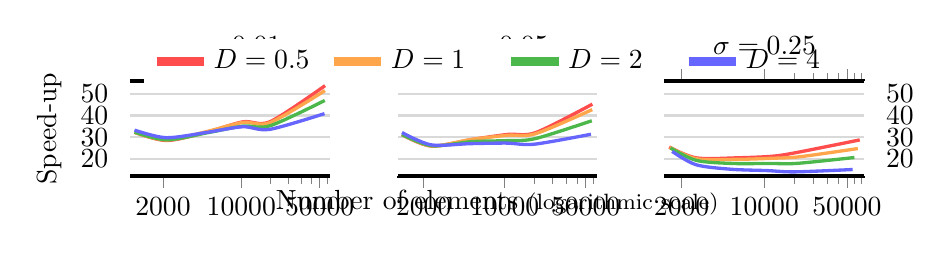
\begin{tikzpicture}
\begin{scope}[shift={(0.0\linewidth,0)}]
\begin{axis}[
 width=0.34\linewidth,height=0.23\linewidth,
 title=\normalsize\mbox{$\sigma=0.01$},
 xmode=log,enlarge x limits=0.025,
 ylabel=Speed-up,
 axis y line*=left,
 ymin=11.8624839129,ymax=56.0132621464,
 tick align=outside,
 x axis line style = ultra thick,y axis line style={white},
 xtick={2000,10000,50000},xticklabels={2000,10000,50000},
 minor xtick={18000,26000,34000,42000,58000,66000}, every y tick/.style={white},ymajorgrids,grid style={gray!30,thick}]
\addplot[very thick,mark=none,smooth,color=red!70] table[] {
	1115.258 32.2252783235
	2153.71966667 28.4233025985
	4981.13166667 32.3616513135
	10376.6173333 37.1198070546
	18148.2636667 37.2211013612
	55929.1186667 53.9108441353
};
\addplot[very thick,mark=none,smooth,color=orange!70] table[] {
	1115.258 32.2252783235
	2153.35533333 28.6797293487
	4966.71566667 32.6400550585
	10369.0493333 36.8487460346
	18133.7363333 36.781442032
	55791.018 51.602071238
};
\addplot[very thick,mark=none,smooth,color=green!60!black!70] table[] {
	1115.04066667 32.3099146422
	2147.23566667 28.7526851328
	4982.24466667 32.0229574612
	10390.4563333 35.1327968955
	18107.314 35.2980375455
	55630.722 47.0337528604
};
\addplot[very thick,mark=none,smooth,color=blue!60!] table[] {
	1114.39433333 33.2486486486
	2129.97033333 29.736042093
	4907.451 32.1786723962
	10285.6763333 34.8070334144
	17956.7793333 33.6131407357
	55294.329 40.9142532147
};
!\end{axis}
\end{scope}
\begin{scope}[shift={(0.28\linewidth,0)}]
\begin{axis}[
 width=0.34\linewidth,height=0.23\linewidth,
 title=\normalsize\mbox{$\sigma=0.05$},
 xmode=log,enlarge x limits=0.025,
 xlabel=Number of elements \footnotesize(logarithmic scale),x label style={at={(axis description cs:0.5,-0.05)},anchor=north},
 yticklabels={},
 legend style={at={(0.55,1.45)},legend style={text width=4em},legend style={draw=none},anchor=north,legend columns=-1},
 axis y line*=left,
 ymin=11.8624839129,ymax=56.0132621464,
 tick align=outside,
 x axis line style = ultra thick,y axis line style={white},
 xtick={2000,10000,50000},xticklabels={2000,10000,50000},
 minor xtick={18000,26000,34000,42000,58000,66000}, every y tick/.style={white},ymajorgrids,grid style={gray!30,thick}]
\addlegendimage{line width=3pt,mark=none,red!70}
\addlegendentry{$D=0.5$}
\addlegendimage{line width=3pt,mark=none,orange!70}
\addlegendentry{$D=1$}
\addlegendimage{line width=3pt,mark=none,green!60!black!70}
\addlegendentry{$D=2$}
\addlegendimage{line width=3pt,mark=none,blue!60!}
\addlegendentry{$D=4$}
\addplot[very thick,mark=none,smooth,color=red!70] table[] {
	1295.23666667 31.1677135678
	2319.814 25.819110884
	5138.91666667 28.8439934399
	10652.52 31.2666106413
	18583.1506667 32.1278454129
	57210.9673333 45.322070276
};
\addplot[very thick,mark=none,smooth,color=orange!70] table[] {
	1303.43733333 31.2462216625
	2325.93266667 25.9383983573
	5118.09633333 28.8854444673
	10641.6626667 30.8565726726
	18521.3283333 31.5976112026
	56982.0486667 42.7786265217
};
\addplot[very thick,mark=none,smooth,color=green!60!black!70] table[] {
	1297.58333333 31.206918239
	2346.43866667 25.9784061697
	5136.495 27.8947264076
	10591.5073333 28.3847510967
	18417.8746667 29.3148284615
	56504.481 37.6052412306
};
\addplot[very thick,mark=none,smooth,color=blue!60!] table[] {
	1298.755 32.1366580311
	2311.45166667 26.419869281
	5030.275 26.9671298515
	10376.187 27.2292105022
	18059.9306667 26.7213832566
	55565.6503333 31.3293406653
};
!\end{axis}
\end{scope}
\begin{scope}[shift={(0.56\linewidth,0)}]
\begin{axis}[
 width=0.34\linewidth,height=0.23\linewidth,
 title=\normalsize\mbox{$\sigma=0.25$},
 xmode=log,enlarge x limits=0.025,
 axis y line*=right,
 ymin=11.8624839129,ymax=56.0132621464,
 tick align=outside,
 x axis line style = ultra thick,y axis line style={white},
 xtick={2000,10000,50000},xticklabels={2000,10000,50000},
 minor xtick={18000,26000,34000,42000,58000,66000}, every y tick/.style={white},ymajorgrids,grid style={gray!30,thick}]
\addplot[very thick,mark=none,smooth,color=red!70] table[] {
	1570.24733333 25.3942307692
	2668.77166667 20.3444849959
	5942.79166667 20.3993484355
	12118.3263333 21.1972603749
	20973.5136667 23.3575518654
	64172.085 28.7048664038
};
\addplot[very thick,mark=none,smooth,color=orange!70] table[] {
	1591.61966667 25.202913109
	2668.32066667 19.9560461416
	5716.86733333 19.6677136596
	11591.0006667 20.1707838397
	20113.2883333 20.9037567014
	61832.7416667 24.6911307363
};
\addplot[very thick,mark=none,smooth,color=green!60!black!70] table[] {
	1610.32533333 24.9646766169
	2667.697 19.1742786165
	5462.71833333 17.7571061136
	10996.7966667 17.7863123745
	18937.3753333 17.8070988432
	57864.3813333 20.5389416945
};
\addplot[very thick,mark=none,smooth,color=blue!60!] table[] {
	1663.819 23.3608007449
	2644.519 17.1872216513
	5240.154 15.073955884
	10558.453 14.4611249278
	18200.8403333 13.8647867807
	55939.5143333 14.9547214638
};
!\end{axis}
\end{scope}
\end{tikzpicture}
\end{center}
\caption{Speed-up results by mesh remodelling - NACA 2412 airfoil}\centering\sffamily\footnotesize
Average of thirty optimisation scenarios\end{figure}

\pagebreak
\subsubsection{Clark-Y}
\vspace*{\fill} \begin{table}[!hp]
\begin{center}
\begin{tabular}{c|cc?c|c?c?c|c|c||c|c}
\multirow{2}{*}{\textbf{\large $\boldsymbol{\sigma}$}} & \multirow{2}{*}{\textbf{\large $\boldsymbol{I}$}} & \multirow{2}{*}{\textbf{\large $\boldsymbol{G}$}} & \multicolumn{2}{c?}{\textbf{\large Generation}} & \multirow{2}{*}{\textbf{\large $\boldsymbol{D}$}} & \multicolumn{5}{c}{\textbf{{\large Remodelling} }} \\\cline{4-5}\cline{7-11}
 & & & \textbf{\# Tri.} & \textbf{Time} & &\textbf{\# Tri.} & \textbf{Time} & \textbf{Preserv.} & \textbf{+ Tri.} & \textbf{Sp.-up} \\\toprule
\multirow{24}[11]{*}{.01} & \multirow{4}{*}{50} & \multirow{4}{*}{1} & \multirow{4}{*}{1052} & \multirow{4}{*}{1.68 ms} & .5 & 1269 & 0.05 ms & 91.31 \% & 20.65 \% & 31.69 \\\cline{6-11}
 & & & &  & 1 & 1264 & 0.05 ms & 91.27 \% & 20.14 \% & 31.61 \\\cline{6-11}
 & & & &  & 2 & 1268 & 0.05 ms & 91.35 \% & 20.56 \% & 31.97 \\\cline{6-11}
 & & & &  & 4 & 1271 & 0.05 ms & 91.50 \% & 20.87 \% & 32.95 \\\cmidrule[1.5pt]{2-11}
 & \multirow{4}{*}{100} & \multirow{4}{*}{2} & \multirow{4}{*}{1850} & \multirow{4}{*}{3.52 ms} & .5 & 2276 & 0.13 ms & 90.20 \% & 23.05 \% & 26.87 \\\cline{6-11}
 & & & &  & 1 & 2292 & 0.13 ms & 90.29 \% & 23.87 \% & 26.88 \\\cline{6-11}
 & & & &  & 2 & 2317 & 0.13 ms & 90.39 \% & 25.25 \% & 26.82 \\\cline{6-11}
 & & & &  & 4 & 2295 & 0.13 ms & 90.40 \% & 24.07 \% & 27.41 \\\cmidrule[1.5pt]{2-11}
 & \multirow{4}{*}{200} & \multirow{4}{*}{4} & \multirow{4}{*}{4627} & \multirow{4}{*}{9.81 ms} & .5 & 5182 & 0.34 ms & 91.36 \% & 12.00 \% & 29.25 \\\cline{6-11}
 & & & &  & 1 & 5161 & 0.33 ms & 91.33 \% & 11.54 \% & 29.44 \\\cline{6-11}
 & & & &  & 2 & 5159 & 0.35 ms & 91.24 \% & 11.50 \% & 28.17 \\\cline{6-11}
 & & & &  & 4 & 5047 & 0.36 ms & 91.05 \% & 9.08 \% & 27.11 \\\cmidrule[1.5pt]{2-11}
 & \multirow{4}{*}{300} & \multirow{4}{*}{6} & \multirow{4}{*}{9833} & \multirow{4}{*}{20.79 ms} & .5 & 10781 & 0.66 ms & 93.53 \% & 9.64 \% & 31.71 \\\cline{6-11}
 & & & &  & 1 & 10724 & 0.67 ms & 93.48 \% & 9.06 \% & 31.07 \\\cline{6-11}
 & & & &  & 2 & 10662 & 0.70 ms & 93.37 \% & 8.43 \% & 29.90 \\\cline{6-11}
 & & & &  & 4 & 10421 & 0.76 ms & 93.10 \% & 5.97 \% & 27.42 \\\cmidrule[1.5pt]{2-11}
 & \multirow{4}{*}{400} & \multirow{4}{*}{8} & \multirow{4}{*}{17337} & \multirow{4}{*}{37.37 ms} & .5 & 18828 & 1.13 ms & 94.86 \% & 8.60 \% & 32.94 \\\cline{6-11}
 & & & &  & 1 & 18701 & 1.16 ms & 94.80 \% & 7.86 \% & 32.28 \\\cline{6-11}
 & & & &  & 2 & 18531 & 1.26 ms & 94.66 \% & 6.88 \% & 29.72 \\\cline{6-11}
 & & & &  & 4 & 18138 & 1.38 ms & 94.37 \% & 4.62 \% & 27.00 \\\cmidrule[1.5pt]{2-11}
 & \multirow{4}{*}{700} & \multirow{4}{*}{14} & \multirow{4}{*}{53738} & \multirow{4}{*}{157.90 ms} & .5 & 57984 & 3.49 ms & 96.77 \% & 7.90 \% & 45.20 \\\cline{6-11}
 & & & &  & 1 & 57488 & 3.72 ms & 96.69 \% & 6.98 \% & 42.39 \\\cline{6-11}
 & & & &  & 2 & 56804 & 4.23 ms & 96.52 \% & 5.71 \% & 37.35 \\\cline{6-11}
 & & & &  & 4 & 55824 & 5.07 ms & 96.18 \% & 3.88 \% & 31.14\\\bottomrule
\end{tabular}\end{center}
\caption{Full results of mesh remodelling for $\sigma=0.01$ - Clark-Y airfoil}\centering\sffamily\footnotesize
Average of thirty optimisation scenarios\end{table}
 \vspace*{\fill}
\begin{table}[!hp]
\begin{center}
\begin{tabular}{c|cc?c|c?c?c|c|c||c|c}
\multirow{2}{*}{\textbf{\large $\boldsymbol{\sigma}$}} & \multirow{2}{*}{\textbf{\large $\boldsymbol{I}$}} & \multirow{2}{*}{\textbf{\large $\boldsymbol{G}$}} & \multicolumn{2}{c?}{\textbf{\large Generation}} & \multirow{2}{*}{\textbf{\large $\boldsymbol{D}$}} & \multicolumn{5}{c}{\textbf{{\large Remodelling} }} \\\cline{4-5}\cline{7-11}
 & & & \textbf{\# Tri.} & \textbf{Time} & &\textbf{\# Tri.} & \textbf{Time} & \textbf{Preserv.} & \textbf{+ Tri.} & \textbf{Sp.-up} \\\toprule
\multirow{24}[13]{*}{.05} & \multirow{4}{*}{50} & \multirow{4}{*}{1} & \multirow{4}{*}{1057} & \multirow{4}{*}{1.68 ms} & .5 & 1386 & 0.06 ms & 91.85 \% & 31.09 \% & 29.81 \\\cline{6-11}
 & & & &  & 1 & 1384 & 0.06 ms & 91.85 \% & 30.87 \% & 29.60 \\\cline{6-11}
 & & & &  & 2 & 1397 & 0.06 ms & 91.97 \% & 32.13 \% & 30.38 \\\cline{6-11}
 & & & &  & 4 & 1381 & 0.05 ms & 91.99 \% & 30.63 \% & 31.08 \\\cmidrule[1.5pt]{2-11}
 & \multirow{4}{*}{100} & \multirow{4}{*}{2} & \multirow{4}{*}{1844} & \multirow{4}{*}{3.49 ms} & .5 & 2377 & 0.14 ms & 90.54 \% & 28.93 \% & 25.43 \\\cline{6-11}
 & & & &  & 1 & 2384 & 0.13 ms & 90.59 \% & 29.33 \% & 26.00 \\\cline{6-11}
 & & & &  & 2 & 2420 & 0.14 ms & 90.75 \% & 31.26 \% & 25.39 \\\cline{6-11}
 & & & &  & 4 & 2398 & 0.14 ms & 90.74 \% & 30.05 \% & 25.37 \\\cmidrule[1.5pt]{2-11}
 & \multirow{4}{*}{200} & \multirow{4}{*}{4} & \multirow{4}{*}{4627} & \multirow{4}{*}{9.55 ms} & .5 & 5279 & 0.35 ms & 91.44 \% & 14.09 \% & 27.40 \\\cline{6-11}
 & & & &  & 1 & 5254 & 0.35 ms & 91.40 \% & 13.56 \% & 27.21 \\\cline{6-11}
 & & & &  & 2 & 5228 & 0.37 ms & 91.28 \% & 13.01 \% & 25.98 \\\cline{6-11}
 & & & &  & 4 & 5081 & 0.39 ms & 90.96 \% & 9.83 \% & 24.26 \\\cmidrule[1.5pt]{2-11}
 & \multirow{4}{*}{300} & \multirow{4}{*}{6} & \multirow{4}{*}{9834} & \multirow{4}{*}{20.30 ms} & .5 & 10966 & 0.69 ms & 93.56 \% & 11.51 \% & 29.28 \\\cline{6-11}
 & & & &  & 1 & 10885 & 0.71 ms & 93.49 \% & 10.69 \% & 28.75 \\\cline{6-11}
 & & & &  & 2 & 10717 & 0.75 ms & 93.29 \% & 8.98 \% & 27.12 \\\cline{6-11}
 & & & &  & 4 & 10439 & 0.83 ms & 92.94 \% & 6.16 \% & 24.37 \\\cmidrule[1.5pt]{2-11}
 & \multirow{4}{*}{400} & \multirow{4}{*}{8} & \multirow{4}{*}{17336} & \multirow{4}{*}{37.06 ms} & .5 & 19098 & 1.19 ms & 94.86 \% & 10.16 \% & 31.21 \\\cline{6-11}
 & & & &  & 1 & 18943 & 1.24 ms & 94.77 \% & 9.27 \% & 29.79 \\\cline{6-11}
 & & & &  & 2 & 18604 & 1.35 ms & 94.57 \% & 7.31 \% & 27.46 \\\cline{6-11}
 & & & &  & 4 & 18175 & 1.55 ms & 94.20 \% & 4.84 \% & 23.86 \\\cmidrule[1.5pt]{2-11}
 & \multirow{4}{*}{700} & \multirow{4}{*}{14} & \multirow{4}{*}{53740} & \multirow{4}{*}{157.14 ms} & .5 & 58814 & 3.72 ms & 96.74 \% & 9.44 \% & 42.21 \\\cline{6-11}
 & & & &  & 1 & 58424 & 4.09 ms & 96.63 \% & 8.72 \% & 38.46 \\\cline{6-11}
 & & & &  & 2 & 56995 & 4.65 ms & 96.41 \% & 6.06 \% & 33.81 \\\cline{6-11}
 & & & &  & 4 & 55852 & 5.81 ms & 96.00 \% & 3.93 \% & 27.05\\\bottomrule
\end{tabular}\end{center}
\caption{Full results of mesh remodelling for $\sigma=0.05$ - Clark-Y airfoil}\centering\sffamily\footnotesize
Average of thirty optimisation scenarios\end{table}

\begin{table}[!hp]
\begin{center}
\begin{tabular}{c|cc?c|c?c?c|c|c||c|c}
\multirow{2}{*}{\textbf{\large $\boldsymbol{\sigma}$}} & \multirow{2}{*}{\textbf{\large $\boldsymbol{I}$}} & \multirow{2}{*}{\textbf{\large $\boldsymbol{G}$}} & \multicolumn{2}{c?}{\textbf{\large Generation}} & \multirow{2}{*}{\textbf{\large $\boldsymbol{D}$}} & \multicolumn{5}{c}{\textbf{{\large Remodelling} }} \\\cline{4-5}\cline{7-11}
 & & & \textbf{\# Tri.} & \textbf{Time} & &\textbf{\# Tri.} & \textbf{Time} & \textbf{Preserv.} & \textbf{+ Tri.} & \textbf{Sp.-up} \\\toprule
\multirow{24}[11]{*}{.25} & \multirow{4}{*}{50} & \multirow{4}{*}{1} & \multirow{4}{*}{1061} & \multirow{4}{*}{1.67 ms} & .5 & 1568 & 0.07 ms & 92.55 \% & 47.84 \% & 24.36 \\\cline{6-11}
 & & & &  & 1 & 1588 & 0.07 ms & 92.64 \% & 49.75 \% & 24.67 \\\cline{6-11}
 & & & &  & 2 & 1607 & 0.07 ms & 92.77 \% & 51.58 \% & 24.35 \\\cline{6-11}
 & & & &  & 4 & 1694 & 0.07 ms & 93.12 \% & 59.69 \% & 22.85 \\\cmidrule[1.5pt]{2-11}
 & \multirow{4}{*}{100} & \multirow{4}{*}{2} & \multirow{4}{*}{1860} & \multirow{4}{*}{3.48 ms} & .5 & 2702 & 0.17 ms & 91.46 \% & 45.28 \% & 20.74 \\\cline{6-11}
 & & & &  & 1 & 2687 & 0.17 ms & 91.38 \% & 44.47 \% & 20.69 \\\cline{6-11}
 & & & &  & 2 & 2684 & 0.18 ms & 91.29 \% & 44.30 \% & 19.69 \\\cline{6-11}
 & & & &  & 4 & 2676 & 0.20 ms & 91.04 \% & 43.88 \% & 17.37 \\\cmidrule[1.5pt]{2-11}
 & \multirow{4}{*}{200} & \multirow{4}{*}{4} & \multirow{4}{*}{4617} & \multirow{4}{*}{9.28 ms} & .5 & 6014 & 0.45 ms & 92.14 \% & 30.27 \% & 20.67 \\\cline{6-11}
 & & & &  & 1 & 5772 & 0.47 ms & 91.72 \% & 25.01 \% & 19.70 \\\cline{6-11}
 & & & &  & 2 & 5507 & 0.52 ms & 91.09 \% & 19.28 \% & 17.84 \\\cline{6-11}
 & & & &  & 4 & 5274 & 0.61 ms & 90.27 \% & 14.24 \% & 15.23 \\\cmidrule[1.5pt]{2-11}
 & \multirow{4}{*}{300} & \multirow{4}{*}{6} & \multirow{4}{*}{9822} & \multirow{4}{*}{19.84 ms} & .5 & 12278 & 0.92 ms & 93.88 \% & 25.00 \% & 21.51 \\\cline{6-11}
 & & & &  & 1 & 11711 & 0.99 ms & 93.47 \% & 19.23 \% & 20.11 \\\cline{6-11}
 & & & &  & 2 & 11073 & 1.11 ms & 92.82 \% & 12.73 \% & 17.82 \\\cline{6-11}
 & & & &  & 4 & 10604 & 1.37 ms & 91.95 \% & 7.96 \% & 14.47 \\\cmidrule[1.5pt]{2-11}
 & \multirow{4}{*}{400} & \multirow{4}{*}{8} & \multirow{4}{*}{17313} & \multirow{4}{*}{36.42 ms} & .5 & 21270 & 1.54 ms & 95.00 \% & 22.86 \% & 23.60 \\\cline{6-11}
 & & & &  & 1 & 20286 & 1.70 ms & 94.63 \% & 17.17 \% & 21.43 \\\cline{6-11}
 & & & &  & 2 & 19096 & 2.07 ms & 93.99 \% & 10.30 \% & 17.58 \\\cline{6-11}
 & & & &  & 4 & 18295 & 2.63 ms & 93.09 \% & 5.67 \% & 13.86 \\\cmidrule[1.5pt]{2-11}
 & \multirow{4}{*}{700} & \multirow{4}{*}{14} & \multirow{4}{*}{53661} & \multirow{4}{*}{154.67 ms} & .5 & 64968 & 5.46 ms & 96.64 \% & 21.07 \% & 28.32 \\\cline{6-11}
 & & & &  & 1 & 62456 & 6.32 ms & 96.31 \% & 16.39 \% & 24.47 \\\cline{6-11}
 & & & &  & 2 & 58286 & 7.58 ms & 95.73 \% & 8.62 \% & 20.41 \\\cline{6-11}
 & & & &  & 4 & 56173 & 10.48 ms & 94.80 \% & 4.68 \% & 14.76\\\bottomrule
\end{tabular}\end{center}
\caption{Full results of mesh remodelling for $\sigma=0.25$ - Clark-Y airfoil}\centering\sffamily\footnotesize
Average of thirty optimisation scenarios\end{table}
 \newpage
\begin{figure}[!h]
\begin{center}
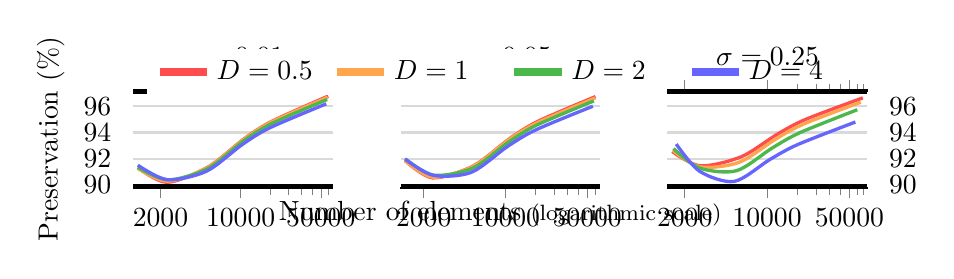
\begin{tikzpicture}
\begin{scope}[shift={(0.0\linewidth,0)}]
\begin{axis}[
 width=0.34\linewidth,height=0.23\linewidth,
 title=\normalsize\mbox{$\sigma=0.01$},
 xmode=log,enlarge x limits=0.025,
 ylabel=Preservation (\%),
 axis y line*=left,
 ymin=89.8717166667,ymax=97.1177141667,
 tick align=outside,
 x axis line style = ultra thick,y axis line style={white},
 xtick={2000,10000,50000},xticklabels={2000,10000,50000},
 minor xtick={18000,26000,34000,42000,58000,66000}, every y tick/.style={white},ymajorgrids,grid style={gray!30,thick}]
\addplot[very thick,mark=none,smooth,color=red!70] table[] {
	1269.16833333 91.3126666667
	2276.448 90.2003333333
	5182.04633333 91.3596666667
	10781.034 93.53
	18828.409 94.8593333333
	57983.79 96.7726666667
};
\addplot[very thick,mark=none,smooth,color=orange!70] table[] {
	1263.86633333 91.2736666667
	2291.61833333 90.285
	5160.89366667 91.328
	10724.269 93.4833333333
	18700.9823333 94.8033333333
	57488.1266667 96.687
};
\addplot[very thick,mark=none,smooth,color=green!60!black!70] table[] {
	1268.27666667 91.35
	2317.154 90.388
	5158.744 91.244
	10661.7936667 93.3703333333
	18531.0873333 94.6646666667
	56804.2343333 96.516
};
\addplot[very thick,mark=none,smooth,color=blue!60!] table[] {
	1271.49233333 91.503
	2295.37766667 90.4013333333
	5046.867 91.0493333333
	10420.654 93.102
	18138.199 94.3706666667
	55823.631 96.183
};
!\end{axis}
\end{scope}
\begin{scope}[shift={(0.28\linewidth,0)}]
\begin{axis}[
 width=0.34\linewidth,height=0.23\linewidth,
 title=\normalsize\mbox{$\sigma=0.05$},
 xmode=log,enlarge x limits=0.025,
 xlabel=Number of elements \footnotesize(logarithmic scale),x label style={at={(axis description cs:0.5,-0.05)},anchor=north},
 yticklabels={},
 legend style={at={(0.55,1.45)},legend style={text width=4em},legend style={draw=none},anchor=north,legend columns=-1},
 axis y line*=left,
 ymin=89.8717166667,ymax=97.1177141667,
 tick align=outside,
 x axis line style = ultra thick,y axis line style={white},
 xtick={2000,10000,50000},xticklabels={2000,10000,50000},
 minor xtick={18000,26000,34000,42000,58000,66000}, every y tick/.style={white},ymajorgrids,grid style={gray!30,thick}]
\addlegendimage{line width=3pt,mark=none,red!70}
\addlegendentry{$D=0.5$}
\addlegendimage{line width=3pt,mark=none,orange!70}
\addlegendentry{$D=1$}
\addlegendimage{line width=3pt,mark=none,green!60!black!70}
\addlegendentry{$D=2$}
\addlegendimage{line width=3pt,mark=none,blue!60!}
\addlegendentry{$D=4$}
\addplot[very thick,mark=none,smooth,color=red!70] table[] {
	1385.864 91.852
	2376.925 90.54
	5278.774 91.4403333333
	10966.038 93.558
	19097.6056667 94.865
	58814.4653333 96.7353333333
};
\addplot[very thick,mark=none,smooth,color=orange!70] table[] {
	1383.557 91.852
	2384.27766667 90.5893333333
	5254.04566667 91.3993333333
	10884.6076667 93.4913333333
	18943.0066667 94.768
	58423.8133333 96.626
};
\addplot[very thick,mark=none,smooth,color=green!60!black!70] table[] {
	1396.929 91.9713333333
	2419.80333333 90.7483333333
	5228.412 91.276
	10716.7823333 93.2896666667
	18603.7346667 94.57
	56994.5426667 96.4066666667
};
\addplot[very thick,mark=none,smooth,color=blue!60!] table[] {
	1381.061 91.9853333333
	2397.538 90.7393333333
	5081.389 90.9563333333
	10439.4216667 92.9413333333
	18174.898 94.1976666667
	55852.1183333 96.0006666667
};
!\end{axis}
\end{scope}
\begin{scope}[shift={(0.56\linewidth,0)}]
\begin{axis}[
 width=0.34\linewidth,height=0.23\linewidth,
 title=\normalsize\mbox{$\sigma=0.25$},
 xmode=log,enlarge x limits=0.025,
 axis y line*=right,
 ymin=89.8717166667,ymax=97.1177141667,
 tick align=outside,
 x axis line style = ultra thick,y axis line style={white},
 xtick={2000,10000,50000},xticklabels={2000,10000,50000},
 minor xtick={18000,26000,34000,42000,58000,66000}, every y tick/.style={white},ymajorgrids,grid style={gray!30,thick}]
\addplot[very thick,mark=none,smooth,color=red!70] table[] {
	1567.82 92.5526666667
	2702.218 91.4586666667
	6014.308 92.141
	12277.662 93.88
	21270.3676667 94.9986666667
	64968.27 96.637
};
\addplot[very thick,mark=none,smooth,color=orange!70] table[] {
	1588.167 92.6406666667
	2687.20233333 91.3796666667
	5771.60766667 91.7186666667
	11710.9023333 93.4676666667
	20285.6003333 94.6296666667
	62456.379 96.3103333333
};
\addplot[very thick,mark=none,smooth,color=green!60!black!70] table[] {
	1607.47966667 92.7696666667
	2683.991 91.286
	5506.855 91.086
	11072.7156667 92.8193333333
	19096.4883333 93.9936666667
	58285.7603333 95.732
};
\addplot[very thick,mark=none,smooth,color=blue!60!] table[] {
	1693.51233333 93.116
	2676.17366667 91.041
	5274.201 90.2713333333
	10604.068 91.9496666667
	18295.141 93.0873333333
	56172.5003333 94.795
};
!\end{axis}
\end{scope}
\end{tikzpicture}
\end{center}
\caption{Element preservation results using mesh remodelling - Clark-Y airfoil}\centering\sffamily\footnotesize
Average of thirty optimisation scenarios\end{figure}

\begin{figure}[!h]
\begin{center}
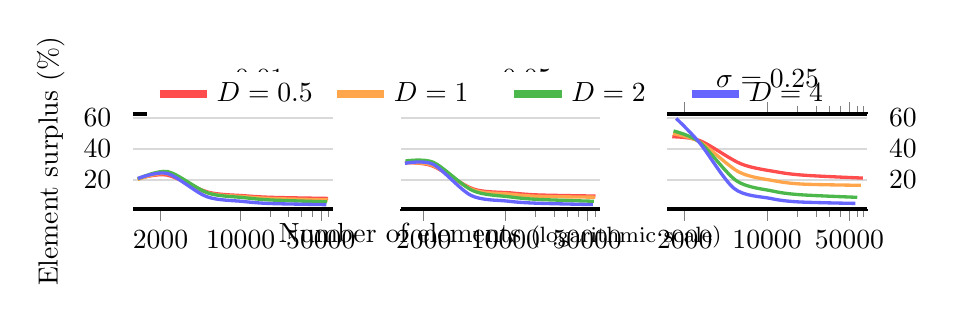
\begin{tikzpicture}
\begin{scope}[shift={(0.0\linewidth,0)}]
\begin{axis}[
 width=0.34\linewidth,height=0.23\linewidth,
 title=\normalsize\mbox{$\sigma=0.01$},
 xmode=log,enlarge x limits=0.025,
 ylabel=Element surplus (\%),
 axis y line*=left,
 ymin=1.09145085224,ymax=62.6174916048,
 tick align=outside,
 x axis line style = ultra thick,y axis line style={white},
 xtick={2000,10000,50000},xticklabels={2000,10000,50000},
 minor xtick={18000,26000,34000,42000,58000,66000}, every y tick/.style={white},ymajorgrids,grid style={gray!30,thick}]
\addplot[very thick,mark=none,smooth,color=red!70] table[] {
	1269.16833333 20.6488825853
	2276.448 23.0503120517
	5182.04633333 11.9998487086
	10781.034 9.63920601302
	18828.409 8.59936224928
	57983.79 7.9015700538
};
\addplot[very thick,mark=none,smooth,color=orange!70] table[] {
	1263.86633333 20.1448671929
	2291.61833333 23.8703238642
	5160.89366667 11.5426749757
	10724.269 9.06192654898
	18700.9823333 7.86438486836
	57488.1266667 6.97919412968
};
\addplot[very thick,mark=none,smooth,color=green!60!black!70] table[] {
	1268.27666667 20.5641195289
	2317.154 25.250619725
	5158.744 11.4962141133
	10661.7936667 8.42657506581
	18531.0873333 6.88445668381
	56804.2343333 5.70654436818
};
\addplot[very thick,mark=none,smooth,color=blue!60!] table[] {
	1271.49233333 20.8698052129
	2295.37766667 24.0735295337
	5046.867 9.07821043911
	10420.654 5.97427210566
	18138.199 4.61833730882
	55823.631 3.88174748501
};
!\end{axis}
\end{scope}
\begin{scope}[shift={(0.28\linewidth,0)}]
\begin{axis}[
 width=0.34\linewidth,height=0.23\linewidth,
 title=\normalsize\mbox{$\sigma=0.05$},
 xmode=log,enlarge x limits=0.025,
 xlabel=Number of elements \footnotesize(logarithmic scale),x label style={at={(axis description cs:0.5,-0.05)},anchor=north},
 yticklabels={},
 legend style={at={(0.55,1.45)},legend style={text width=4em},legend style={draw=none},anchor=north,legend columns=-1},
 axis y line*=left,
 ymin=1.09145085224,ymax=62.6174916048,
 tick align=outside,
 x axis line style = ultra thick,y axis line style={white},
 xtick={2000,10000,50000},xticklabels={2000,10000,50000},
 minor xtick={18000,26000,34000,42000,58000,66000}, every y tick/.style={white},ymajorgrids,grid style={gray!30,thick}]
\addlegendimage{line width=3pt,mark=none,red!70}
\addlegendentry{$D=0.5$}
\addlegendimage{line width=3pt,mark=none,orange!70}
\addlegendentry{$D=1$}
\addlegendimage{line width=3pt,mark=none,green!60!black!70}
\addlegendentry{$D=2$}
\addlegendimage{line width=3pt,mark=none,blue!60!}
\addlegendentry{$D=4$}
\addplot[very thick,mark=none,smooth,color=red!70] table[] {
	1385.864 31.0869587836
	2376.925 28.9324181874
	5278.774 14.0945389049
	10966.038 11.5141957066
	19097.6056667 10.1602245812
	58814.4653333 9.44232992405
};
\addplot[very thick,mark=none,smooth,color=orange!70] table[] {
	1383.557 30.8687428448
	2384.27766667 29.3312515934
	5254.04566667 13.5600648415
	10884.6076667 10.6861265235
	18943.0066667 9.26845517005
	58423.8133333 8.71540220606
};
\addplot[very thick,mark=none,smooth,color=green!60!black!70] table[] {
	1396.929 32.1335818281
	2419.80333333 31.2582834144
	5228.412 13.0060230548
	10716.7823333 8.97950221073
	18603.7346667 7.31144127174
	56994.5426667 6.05580628922
};
\addplot[very thick,mark=none,smooth,color=blue!60!] table[] {
	1381.061 30.6326496573
	2397.538 30.0505367381
	5081.389 9.8282925072
	10439.4216667 6.15900754676
	18174.898 4.83779382435
	55852.1183333 3.92997584779
};
!\end{axis}
\end{scope}
\begin{scope}[shift={(0.56\linewidth,0)}]
\begin{axis}[
 width=0.34\linewidth,height=0.23\linewidth,
 title=\normalsize\mbox{$\sigma=0.25$},
 xmode=log,enlarge x limits=0.025,
 axis y line*=right,
 ymin=1.09145085224,ymax=62.6174916048,
 tick align=outside,
 x axis line style = ultra thick,y axis line style={white},
 xtick={2000,10000,50000},xticklabels={2000,10000,50000},
 minor xtick={18000,26000,34000,42000,58000,66000}, every y tick/.style={white},ymajorgrids,grid style={gray!30,thick}]
\addplot[very thick,mark=none,smooth,color=red!70] table[] {
	1567.82 47.8356748574
	2702.218 45.2785068596
	6014.308 30.2691730707
	12277.662 24.9988537893
	21270.3676667 22.8580201517
	64968.27 21.0714976824
};
\addplot[very thick,mark=none,smooth,color=orange!70] table[] {
	1588.167 49.7542704082
	2687.20233333 44.4712242374
	5771.60766667 25.0123136402
	11710.9023333 19.2286746862
	20285.6003333 17.1699866029
	62456.379 16.3904679215
};
\addplot[very thick,mark=none,smooth,color=green!60!black!70] table[] {
	1607.47966667 51.5753347586
	2683.991 44.298574321
	5506.855 19.2778033765
	11072.7156667 12.7312974301
	19096.4883333 10.3016546423
	58285.7603333 8.61831932906
};
\addplot[very thick,mark=none,smooth,color=blue!60!] table[] {
	1693.51233333 59.6876801404
	2676.17366667 43.8782934575
	5274.201 14.238546293
	10604.068 7.95999641493
	18295.141 5.67305826025
	56172.5003333 4.68015762039
};
!\end{axis}
\end{scope}
\end{tikzpicture}
\end{center}
\caption{Element surplus results on meshes from mesh remodelling - Clark-Y airfoil}\centering\sffamily\footnotesize
Average of thirty optimisation scenarios\end{figure}

\begin{figure}[!h]
\begin{center}
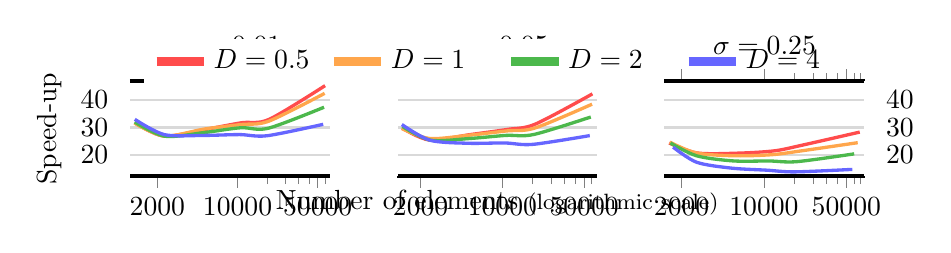
\begin{tikzpicture}
\begin{scope}[shift={(0.0\linewidth,0)}]
\begin{axis}[
 width=0.34\linewidth,height=0.23\linewidth,
 title=\normalsize\mbox{$\sigma=0.01$},
 xmode=log,enlarge x limits=0.025,
 ylabel=Speed-up,
 axis y line*=left,
 ymin=12.298001935,ymax=46.8477530579,
 tick align=outside,
 x axis line style = ultra thick,y axis line style={white},
 xtick={2000,10000,50000},xticklabels={2000,10000,50000},
 minor xtick={18000,26000,34000,42000,58000,66000}, every y tick/.style={white},ymajorgrids,grid style={gray!30,thick}]
\addplot[very thick,mark=none,smooth,color=red!70] table[] {
	1269.16833333 31.6855345912
	2276.448 26.8707707962
	5182.04633333 29.2477146264
	10781.034 31.7074162558
	18828.409 32.9383318154
	57983.79 45.202526814
};
\addplot[very thick,mark=none,smooth,color=orange!70] table[] {
	1263.86633333 31.6060225847
	2291.61833333 26.8776081425
	5160.89366667 29.4407881576
	10724.269 31.0678354418
	18700.9823333 32.2773651178
	57488.1266667 42.3926903045
};
\addplot[very thick,mark=none,smooth,color=green!60!black!70] table[] {
	1268.27666667 31.9670050761
	2317.154 26.8161970043
	5158.744 28.1727603369
	10661.7936667 29.8974309816
	18531.0873333 29.7190647863
	56804.2343333 37.3539723219
};
\addplot[very thick,mark=none,smooth,color=blue!60!] table[] {
	1271.49233333 32.9496402878
	2295.37766667 27.407628438
	5046.867 27.1089519248
	10420.654 27.4152858964
	18138.199 27.0006743413
	55823.631 31.1383365433
};
!\end{axis}
\end{scope}
\begin{scope}[shift={(0.28\linewidth,0)}]
\begin{axis}[
 width=0.34\linewidth,height=0.23\linewidth,
 title=\normalsize\mbox{$\sigma=0.05$},
 xmode=log,enlarge x limits=0.025,
 xlabel=Number of elements \footnotesize(logarithmic scale),x label style={at={(axis description cs:0.5,-0.05)},anchor=north},
 yticklabels={},
 legend style={at={(0.55,1.45)},legend style={text width=4em},legend style={draw=none},anchor=north,legend columns=-1},
 axis y line*=left,
 ymin=12.298001935,ymax=46.8477530579,
 tick align=outside,
 x axis line style = ultra thick,y axis line style={white},
 xtick={2000,10000,50000},xticklabels={2000,10000,50000},
 minor xtick={18000,26000,34000,42000,58000,66000}, every y tick/.style={white},ymajorgrids,grid style={gray!30,thick}]
\addlegendimage{line width=3pt,mark=none,red!70}
\addlegendentry{$D=0.5$}
\addlegendimage{line width=3pt,mark=none,orange!70}
\addlegendentry{$D=1$}
\addlegendimage{line width=3pt,mark=none,green!60!black!70}
\addlegendentry{$D=2$}
\addlegendimage{line width=3pt,mark=none,blue!60!}
\addlegendentry{$D=4$}
\addplot[very thick,mark=none,smooth,color=red!70] table[] {
	1385.864 29.8071005917
	2376.925 25.4262493935
	5278.774 27.4042288557
	10966.038 29.2777323652
	19097.6056667 31.2138004604
	58814.4653333 42.2111672218
};
\addplot[very thick,mark=none,smooth,color=orange!70] table[] {
	1383.557 29.5969447709
	2384.27766667 26.0002480774
	5254.04566667 27.2115713471
	10884.6076667 28.746943015
	18943.0066667 29.7920261508
	58423.8133333 38.4640840704
};
\addplot[very thick,mark=none,smooth,color=green!60!black!70] table[] {
	1396.929 30.3823884198
	2419.80333333 25.3892926357
	5228.412 25.9846684206
	10716.7823333 27.1159652639
	18603.7346667 27.459017608
	56994.5426667 33.8062258428
};
\addplot[very thick,mark=none,smooth,color=blue!60!] table[] {
	1381.061 31.075879087
	2397.538 25.3708545146
	5081.389 24.2571985095
	10439.4216667 24.367256283
	18174.898 23.8584241696
	55852.1183333 27.0495972092
};
!\end{axis}
\end{scope}
\begin{scope}[shift={(0.56\linewidth,0)}]
\begin{axis}[
 width=0.34\linewidth,height=0.23\linewidth,
 title=\normalsize\mbox{$\sigma=0.25$},
 xmode=log,enlarge x limits=0.025,
 axis y line*=right,
 ymin=12.298001935,ymax=46.8477530579,
 tick align=outside,
 x axis line style = ultra thick,y axis line style={white},
 xtick={2000,10000,50000},xticklabels={2000,10000,50000},
 minor xtick={18000,26000,34000,42000,58000,66000}, every y tick/.style={white},ymajorgrids,grid style={gray!30,thick}]
\addplot[very thick,mark=none,smooth,color=red!70] table[] {
	1567.82 24.3597087379
	2702.218 20.7384125721
	6014.308 20.6685714286
	12277.662 21.5144055236
	21270.3676667 23.5989934336
	64968.27 28.321400669
};
\addplot[very thick,mark=none,smooth,color=orange!70] table[] {
	1588.167 24.6710914454
	2687.20233333 20.6931321953
	5771.60766667 19.7048959955
	11710.9023333 20.1133153092
	20285.6003333 21.433680576
	62456.379 24.4699482658
};
\addplot[very thick,mark=none,smooth,color=green!60!black!70] table[] {
	1607.47966667 24.3478893741
	2683.991 19.6924820552
	5506.855 17.8394183961
	11072.7156667 17.8210863576
	19096.4883333 17.5816127838
	58285.7603333 20.4091672825
};
\addplot[very thick,mark=none,smooth,color=blue!60!] table[] {
	1693.51233333 22.8510928962
	2676.17366667 17.372437927
	5274.201 15.234055355
	10604.068 14.470046195
	18295.141 13.8648840721
	56172.5003333 14.7614343841
};
!\end{axis}
\end{scope}
\end{tikzpicture}
\end{center}
\caption{Speed-up results by mesh remodelling - Clark-Y airfoil}\centering\sffamily\footnotesize
Average of thirty optimisation scenarios\end{figure}

\pagebreak
\subsubsection{Boeing 737}
\vspace*{\fill} \begin{table}[!hp]
\begin{center}
\begin{tabular}{c|cc?c|c?c?c|c|c||c|c}
\multirow{2}{*}{\textbf{\large $\boldsymbol{\sigma}$}} & \multirow{2}{*}{\textbf{\large $\boldsymbol{I}$}} & \multirow{2}{*}{\textbf{\large $\boldsymbol{G}$}} & \multicolumn{2}{c?}{\textbf{\large Generation}} & \multirow{2}{*}{\textbf{\large $\boldsymbol{D}$}} & \multicolumn{5}{c}{\textbf{{\large Remodelling} }} \\\cline{4-5}\cline{7-11}
 & & & \textbf{\# Tri.} & \textbf{Time} & &\textbf{\# Tri.} & \textbf{Time} & \textbf{Preserv.} & \textbf{+ Tri.} & \textbf{Sp.-up} \\\toprule
\multirow{24}[11]{*}{.01} & \multirow{4}{*}{50} & \multirow{4}{*}{1} & \multirow{4}{*}{1167} & \multirow{4}{*}{1.78 ms} & .5 & 1182 & 0.05 ms & 90.97 \% & 1.24 \% & 34.92 \\\cline{6-11}
 & & & &  & 1 & 1182 & 0.05 ms & 90.97 \% & 1.24 \% & 34.99 \\\cline{6-11}
 & & & &  & 2 & 1184 & 0.05 ms & 90.99 \% & 1.47 \% & 35.11 \\\cline{6-11}
 & & & &  & 4 & 1192 & 0.05 ms & 91.15 \% & 2.11 \% & 36.38 \\\cmidrule[1.5pt]{2-11}
 & \multirow{4}{*}{100} & \multirow{4}{*}{2} & \multirow{4}{*}{1864} & \multirow{4}{*}{3.42 ms} & .5 & 2215 & 0.12 ms & 89.98 \% & 18.86 \% & 27.65 \\\cline{6-11}
 & & & &  & 1 & 2217 & 0.12 ms & 90.00 \% & 18.95 \% & 27.64 \\\cline{6-11}
 & & & &  & 2 & 2229 & 0.12 ms & 90.07 \% & 19.60 \% & 27.86 \\\cline{6-11}
 & & & &  & 4 & 2228 & 0.12 ms & 90.19 \% & 19.53 \% & 28.44 \\\cmidrule[1.5pt]{2-11}
 & \multirow{4}{*}{200} & \multirow{4}{*}{4} & \multirow{4}{*}{4716} & \multirow{4}{*}{9.56 ms} & .5 & 5182 & 0.32 ms & 91.46 \% & 9.87 \% & 30.26 \\\cline{6-11}
 & & & &  & 1 & 5156 & 0.31 ms & 91.43 \% & 9.32 \% & 30.80 \\\cline{6-11}
 & & & &  & 2 & 5150 & 0.32 ms & 91.38 \% & 9.21 \% & 29.66 \\\cline{6-11}
 & & & &  & 4 & 5054 & 0.31 ms & 91.30 \% & 7.16 \% & 30.63 \\\cmidrule[1.5pt]{2-11}
 & \multirow{4}{*}{300} & \multirow{4}{*}{6} & \multirow{4}{*}{9982} & \multirow{4}{*}{20.06 ms} & .5 & 10894 & 0.62 ms & 93.71 \% & 9.14 \% & 32.25 \\\cline{6-11}
 & & & &  & 1 & 10845 & 0.63 ms & 93.66 \% & 8.65 \% & 32.01 \\\cline{6-11}
 & & & &  & 2 & 10788 & 0.66 ms & 93.60 \% & 8.08 \% & 30.42 \\\cline{6-11}
 & & & &  & 4 & 10584 & 0.68 ms & 93.45 \% & 6.04 \% & 29.38 \\\cmidrule[1.5pt]{2-11}
 & \multirow{4}{*}{400} & \multirow{4}{*}{8} & \multirow{4}{*}{17626} & \multirow{4}{*}{36.61 ms} & .5 & 19120 & 1.09 ms & 95.04 \% & 8.47 \% & 33.47 \\\cline{6-11}
 & & & &  & 1 & 18986 & 1.11 ms & 94.99 \% & 7.71 \% & 32.94 \\\cline{6-11}
 & & & &  & 2 & 18838 & 1.17 ms & 94.90 \% & 6.88 \% & 31.31 \\\cline{6-11}
 & & & &  & 4 & 18490 & 1.25 ms & 94.72 \% & 4.90 \% & 29.31 \\\cmidrule[1.5pt]{2-11}
 & \multirow{4}{*}{700} & \multirow{4}{*}{14} & \multirow{4}{*}{54768} & \multirow{4}{*}{158.33 ms} & .5 & 59055 & 3.31 ms & 96.89 \% & 7.83 \% & 47.84 \\\cline{6-11}
 & & & &  & 1 & 58578 & 3.44 ms & 96.84 \% & 6.96 \% & 45.97 \\\cline{6-11}
 & & & &  & 2 & 57903 & 3.71 ms & 96.73 \% & 5.72 \% & 42.68 \\\cline{6-11}
 & & & &  & 4 & 56903 & 4.32 ms & 96.51 \% & 3.90 \% & 36.68\\\bottomrule
\end{tabular}\end{center}
\caption{Full results of mesh remodelling for $\sigma=0.01$ - Boeing 737 airfoil}\centering\sffamily\footnotesize
Average of thirty optimisation scenarios\end{table}
 \vspace*{\fill}
\begin{table}[!hp]
\begin{center}
\begin{tabular}{c|cc?c|c?c?c|c|c||c|c}
\multirow{2}{*}{\textbf{\large $\boldsymbol{\sigma}$}} & \multirow{2}{*}{\textbf{\large $\boldsymbol{I}$}} & \multirow{2}{*}{\textbf{\large $\boldsymbol{G}$}} & \multicolumn{2}{c?}{\textbf{\large Generation}} & \multirow{2}{*}{\textbf{\large $\boldsymbol{D}$}} & \multicolumn{5}{c}{\textbf{{\large Remodelling} }} \\\cline{4-5}\cline{7-11}
 & & & \textbf{\# Tri.} & \textbf{Time} & &\textbf{\# Tri.} & \textbf{Time} & \textbf{Preserv.} & \textbf{+ Tri.} & \textbf{Sp.-up} \\\toprule
\multirow{24}[13]{*}{.05} & \multirow{4}{*}{50} & \multirow{4}{*}{1} & \multirow{4}{*}{1165} & \multirow{4}{*}{1.78 ms} & .5 & 1280 & 0.05 ms & 91.48 \% & 9.81 \% & 33.55 \\\cline{6-11}
 & & & &  & 1 & 1279 & 0.05 ms & 91.47 \% & 9.73 \% & 33.46 \\\cline{6-11}
 & & & &  & 2 & 1317 & 0.05 ms & 91.71 \% & 12.99 \% & 34.04 \\\cline{6-11}
 & & & &  & 4 & 1310 & 0.05 ms & 91.78 \% & 12.44 \% & 34.50 \\\cmidrule[1.5pt]{2-11}
 & \multirow{4}{*}{100} & \multirow{4}{*}{2} & \multirow{4}{*}{1864} & \multirow{4}{*}{3.41 ms} & .5 & 2390 & 0.13 ms & 90.59 \% & 28.20 \% & 25.95 \\\cline{6-11}
 & & & &  & 1 & 2411 & 0.13 ms & 90.67 \% & 29.31 \% & 26.13 \\\cline{6-11}
 & & & &  & 2 & 2404 & 0.13 ms & 90.69 \% & 28.93 \% & 26.03 \\\cline{6-11}
 & & & &  & 4 & 2416 & 0.13 ms & 90.83 \% & 29.58 \% & 26.55 \\\cmidrule[1.5pt]{2-11}
 & \multirow{4}{*}{200} & \multirow{4}{*}{4} & \multirow{4}{*}{4717} & \multirow{4}{*}{9.20 ms} & .5 & 5291 & 0.34 ms & 91.50 \% & 12.16 \% & 27.31 \\\cline{6-11}
 & & & &  & 1 & 5293 & 0.34 ms & 91.50 \% & 12.20 \% & 26.80 \\\cline{6-11}
 & & & &  & 2 & 5296 & 0.35 ms & 91.46 \% & 12.27 \% & 26.09 \\\cline{6-11}
 & & & &  & 4 & 5161 & 0.36 ms & 91.27 \% & 9.41 \% & 25.91 \\\cmidrule[1.5pt]{2-11}
 & \multirow{4}{*}{300} & \multirow{4}{*}{6} & \multirow{4}{*}{9982} & \multirow{4}{*}{19.73 ms} & .5 & 11085 & 0.69 ms & 93.68 \% & 11.06 \% & 28.43 \\\cline{6-11}
 & & & &  & 1 & 11011 & 0.70 ms & 93.63 \% & 10.31 \% & 28.25 \\\cline{6-11}
 & & & &  & 2 & 10928 & 0.73 ms & 93.54 \% & 9.48 \% & 27.21 \\\cline{6-11}
 & & & &  & 4 & 10652 & 0.77 ms & 93.27 \% & 6.71 \% & 25.47 \\\cmidrule[1.5pt]{2-11}
 & \multirow{4}{*}{400} & \multirow{4}{*}{8} & \multirow{4}{*}{17627} & \multirow{4}{*}{36.40 ms} & .5 & 19376 & 1.22 ms & 94.97 \% & 9.92 \% & 29.74 \\\cline{6-11}
 & & & &  & 1 & 19272 & 1.25 ms & 94.92 \% & 9.33 \% & 29.20 \\\cline{6-11}
 & & & &  & 2 & 18999 & 1.32 ms & 94.79 \% & 7.78 \% & 27.49 \\\cline{6-11}
 & & & &  & 4 & 18521 & 1.46 ms & 94.50 \% & 5.07 \% & 24.99 \\\cmidrule[1.5pt]{2-11}
 & \multirow{4}{*}{700} & \multirow{4}{*}{14} & \multirow{4}{*}{54755} & \multirow{4}{*}{157.51 ms} & .5 & 59893 & 3.69 ms & 96.82 \% & 9.38 \% & 42.66 \\\cline{6-11}
 & & & &  & 1 & 59538 & 3.96 ms & 96.74 \% & 8.74 \% & 39.81 \\\cline{6-11}
 & & & &  & 2 & 58279 & 4.30 ms & 96.60 \% & 6.44 \% & 36.62 \\\cline{6-11}
 & & & &  & 4 & 56986 & 5.19 ms & 96.27 \% & 4.08 \% & 30.35\\\bottomrule
\end{tabular}\end{center}
\caption{Full results of mesh remodelling for $\sigma=0.05$ - Boeing 737 airfoil}\centering\sffamily\footnotesize
Average of thirty optimisation scenarios\end{table}

\begin{table}[!hp]
\begin{center}
\begin{tabular}{c|cc?c|c?c?c|c|c||c|c}
\multirow{2}{*}{\textbf{\large $\boldsymbol{\sigma}$}} & \multirow{2}{*}{\textbf{\large $\boldsymbol{I}$}} & \multirow{2}{*}{\textbf{\large $\boldsymbol{G}$}} & \multicolumn{2}{c?}{\textbf{\large Generation}} & \multirow{2}{*}{\textbf{\large $\boldsymbol{D}$}} & \multicolumn{5}{c}{\textbf{{\large Remodelling} }} \\\cline{4-5}\cline{7-11}
 & & & \textbf{\# Tri.} & \textbf{Time} & &\textbf{\# Tri.} & \textbf{Time} & \textbf{Preserv.} & \textbf{+ Tri.} & \textbf{Sp.-up} \\\toprule
\multirow{24}[13]{*}{.25} & \multirow{4}{*}{50} & \multirow{4}{*}{1} & \multirow{4}{*}{1172} & \multirow{4}{*}{1.78 ms} & .5 & 1646 & 0.07 ms & 92.82 \% & 40.50 \% & 26.26 \\\cline{6-11}
 & & & &  & 1 & 1663 & 0.07 ms & 92.94 \% & 41.94 \% & 25.52 \\\cline{6-11}
 & & & &  & 2 & 1689 & 0.07 ms & 92.99 \% & 44.13 \% & 25.79 \\\cline{6-11}
 & & & &  & 4 & 1801 & 0.08 ms & 93.38 \% & 53.73 \% & 23.76 \\\cmidrule[1.5pt]{2-11}
 & \multirow{4}{*}{100} & \multirow{4}{*}{2} & \multirow{4}{*}{1859} & \multirow{4}{*}{3.39 ms} & .5 & 2810 & 0.17 ms & 91.71 \% & 51.15 \% & 20.31 \\\cline{6-11}
 & & & &  & 1 & 2790 & 0.17 ms & 91.62 \% & 50.07 \% & 19.89 \\\cline{6-11}
 & & & &  & 2 & 2773 & 0.18 ms & 91.48 \% & 49.11 \% & 19.13 \\\cline{6-11}
 & & & &  & 4 & 2773 & 0.20 ms & 91.23 \% & 49.14 \% & 16.82 \\\cmidrule[1.5pt]{2-11}
 & \multirow{4}{*}{200} & \multirow{4}{*}{4} & \multirow{4}{*}{4715} & \multirow{4}{*}{9.06 ms} & .5 & 6177 & 0.45 ms & 92.32 \% & 31.02 \% & 19.92 \\\cline{6-11}
 & & & &  & 1 & 5894 & 0.47 ms & 91.88 \% & 25.02 \% & 19.37 \\\cline{6-11}
 & & & &  & 2 & 5655 & 0.52 ms & 91.28 \% & 19.94 \% & 17.57 \\\cline{6-11}
 & & & &  & 4 & 5387 & 0.60 ms & 90.45 \% & 14.26 \% & 15.04 \\\cmidrule[1.5pt]{2-11}
 & \multirow{4}{*}{300} & \multirow{4}{*}{6} & \multirow{4}{*}{9974} & \multirow{4}{*}{19.53 ms} & .5 & 12514 & 0.92 ms & 94.00 \% & 25.47 \% & 21.22 \\\cline{6-11}
 & & & &  & 1 & 11932 & 0.99 ms & 93.59 \% & 19.63 \% & 19.82 \\\cline{6-11}
 & & & &  & 2 & 11316 & 1.11 ms & 92.97 \% & 13.45 \% & 17.57 \\\cline{6-11}
 & & & &  & 4 & 10820 & 1.36 ms & 92.10 \% & 8.48 \% & 14.34 \\\cmidrule[1.5pt]{2-11}
 & \multirow{4}{*}{400} & \multirow{4}{*}{8} & \multirow{4}{*}{17610} & \multirow{4}{*}{36.04 ms} & .5 & 21685 & 1.57 ms & 95.09 \% & 23.14 \% & 22.99 \\\cline{6-11}
 & & & &  & 1 & 20686 & 1.72 ms & 94.71 \% & 17.47 \% & 20.99 \\\cline{6-11}
 & & & &  & 2 & 19525 & 2.03 ms & 94.11 \% & 10.87 \% & 17.78 \\\cline{6-11}
 & & & &  & 4 & 18649 & 2.62 ms & 93.21 \% & 5.90 \% & 13.78 \\\cmidrule[1.5pt]{2-11}
 & \multirow{4}{*}{700} & \multirow{4}{*}{14} & \multirow{4}{*}{54727} & \multirow{4}{*}{156.47 ms} & .5 & 66406 & 5.46 ms & 96.69 \% & 21.34 \% & 28.66 \\\cline{6-11}
 & & & &  & 1 & 63703 & 6.31 ms & 96.35 \% & 16.40 \% & 24.80 \\\cline{6-11}
 & & & &  & 2 & 59598 & 7.52 ms & 95.81 \% & 8.90 \% & 20.82 \\\cline{6-11}
 & & & &  & 4 & 57326 & 10.38 ms & 94.88 \% & 4.75 \% & 15.08\\\bottomrule
\end{tabular}\end{center}
\caption{Full results of mesh remodelling for $\sigma=0.25$ - Boeing 737 airfoil}\centering\sffamily\footnotesize
Average of thirty optimisation scenarios\end{table}
 \newpage
\begin{figure}[!h]
\begin{center}
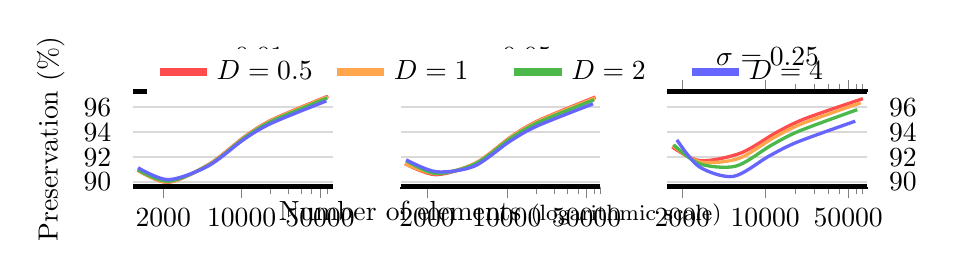
\begin{tikzpicture}
\begin{scope}[shift={(0.0\linewidth,0)}]
\begin{axis}[
 width=0.34\linewidth,height=0.23\linewidth,
 title=\normalsize\mbox{$\sigma=0.01$},
 xmode=log,enlarge x limits=0.025,
 ylabel=Preservation (\%),
 axis y line*=left,
 ymin=89.635,ymax=97.25695,
 tick align=outside,
 x axis line style = ultra thick,y axis line style={white},
 xtick={2000,10000,50000},xticklabels={2000,10000,50000},
 minor xtick={18000,26000,34000,42000,58000,66000}, every y tick/.style={white},ymajorgrids,grid style={gray!30,thick}]
\addplot[very thick,mark=none,smooth,color=red!70] table[] {
	1181.62066667 90.969
	2215.46 89.9806666667
	5181.616 91.459
	10893.6296667 93.7076666667
	19119.5003333 95.038
	59054.826 96.894
};
\addplot[very thick,mark=none,smooth,color=orange!70] table[] {
	1181.62066667 90.969
	2217.06433333 90.001
	5155.626 91.4273333333
	10845.362 93.662
	18986.0146667 94.9903333333
	58578.4676667 96.8403333333
};
\addplot[very thick,mark=none,smooth,color=green!60!black!70] table[] {
	1184.32666667 90.989
	2229.279 90.0676666667
	5150.313 91.38
	10787.995 93.599
	18838.031 94.905
	57902.6766667 96.7316666667
};
\addplot[very thick,mark=none,smooth,color=blue!60!] table[] {
	1191.78133333 91.146
	2227.87566667 90.1936666667
	5053.76633333 91.3006666667
	10584.265 93.4486666667
	18489.5223333 94.724
	56902.9196667 96.5066666667
};
!\end{axis}
\end{scope}
\begin{scope}[shift={(0.28\linewidth,0)}]
\begin{axis}[
 width=0.34\linewidth,height=0.23\linewidth,
 title=\normalsize\mbox{$\sigma=0.05$},
 xmode=log,enlarge x limits=0.025,
 xlabel=Number of elements \footnotesize(logarithmic scale),x label style={at={(axis description cs:0.5,-0.05)},anchor=north},
 yticklabels={},
 legend style={at={(0.55,1.45)},legend style={text width=4em},legend style={draw=none},anchor=north,legend columns=-1},
 axis y line*=left,
 ymin=89.635,ymax=97.25695,
 tick align=outside,
 x axis line style = ultra thick,y axis line style={white},
 xtick={2000,10000,50000},xticklabels={2000,10000,50000},
 minor xtick={18000,26000,34000,42000,58000,66000}, every y tick/.style={white},ymajorgrids,grid style={gray!30,thick}]
\addlegendimage{line width=3pt,mark=none,red!70}
\addlegendentry{$D=0.5$}
\addlegendimage{line width=3pt,mark=none,orange!70}
\addlegendentry{$D=1$}
\addlegendimage{line width=3pt,mark=none,green!60!black!70}
\addlegendentry{$D=2$}
\addlegendimage{line width=3pt,mark=none,blue!60!}
\addlegendentry{$D=4$}
\addplot[very thick,mark=none,smooth,color=red!70] table[] {
	1279.641 91.4773333333
	2390.32533333 90.5906666667
	5290.78533333 91.504
	11085.4573333 93.683
	19376.218 94.9713333333
	59892.9113333 96.8196666667
};
\addplot[very thick,mark=none,smooth,color=orange!70] table[] {
	1278.69166667 91.4746666667
	2410.959 90.6716666667
	5292.737 91.501
	11011.373 93.633
	19272.0743333 94.9203333333
	59537.7083333 96.7386666667
};
\addplot[very thick,mark=none,smooth,color=green!60!black!70] table[] {
	1316.78633333 91.7136666667
	2403.786 90.687
	5295.75033333 91.459
	10928.2076667 93.538
	18998.6893333 94.7936666667
	58278.8796667 96.599
};
\addplot[very thick,mark=none,smooth,color=blue!60!] table[] {
	1310.299 91.7836666667
	2415.94733333 90.8263333333
	5160.93433333 91.268
	10652.052 93.2716666667
	18520.5773333 94.5046666667
	56986.4536667 96.2736666667
};
!\end{axis}
\end{scope}
\begin{scope}[shift={(0.56\linewidth,0)}]
\begin{axis}[
 width=0.34\linewidth,height=0.23\linewidth,
 title=\normalsize\mbox{$\sigma=0.25$},
 xmode=log,enlarge x limits=0.025,
 axis y line*=right,
 ymin=89.635,ymax=97.25695,
 tick align=outside,
 x axis line style = ultra thick,y axis line style={white},
 xtick={2000,10000,50000},xticklabels={2000,10000,50000},
 minor xtick={18000,26000,34000,42000,58000,66000}, every y tick/.style={white},ymajorgrids,grid style={gray!30,thick}]
\addplot[very thick,mark=none,smooth,color=red!70] table[] {
	1646.15933333 92.8183333333
	2810.362 91.7126666667
	6177.13333333 92.3163333333
	12514.3133333 93.997
	21685.3016667 95.088
	66406.0556667 96.6856666667
};
\addplot[very thick,mark=none,smooth,color=orange!70] table[] {
	1663.08533333 92.936
	2790.36366667 91.6196666667
	5894.47266667 91.875
	11932.3566667 93.5886666667
	20686.2586667 94.706
	63703.007 96.3536666667
};
\addplot[very thick,mark=none,smooth,color=green!60!black!70] table[] {
	1688.79933333 92.9936666667
	2772.61566667 91.4773333333
	5654.935 91.2786666667
	11315.806 92.968
	19524.696 94.1093333333
	59597.5723333 95.8066666667
};
\addplot[very thick,mark=none,smooth,color=blue!60!] table[] {
	1801.26033333 93.3823333333
	2773.10966667 91.2313333333
	5387.17566667 90.4546666667
	10819.9246667 92.096
	18649.48 93.2103333333
	57325.7383333 94.8823333333
};
!\end{axis}
\end{scope}
\end{tikzpicture}
\end{center}
\caption{Element preservation results using mesh remodelling - Boeing 737 airfoil}\centering\sffamily\footnotesize
Average of thirty optimisation scenarios\end{figure}

\begin{figure}[!h]
\begin{center}
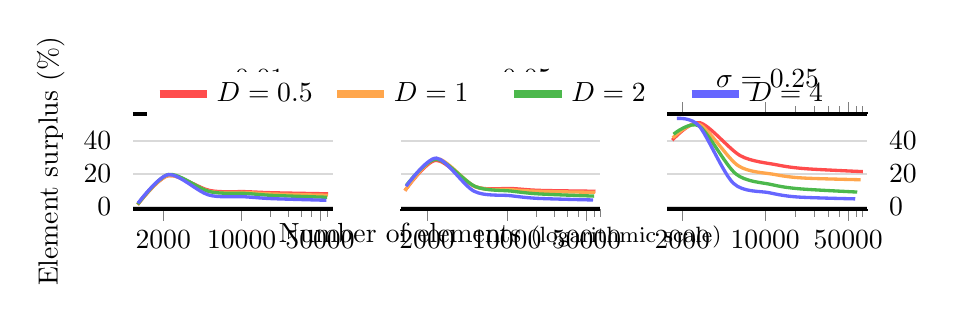
\begin{tikzpicture}
\begin{scope}[shift={(0.0\linewidth,0)}]
\begin{axis}[
 width=0.34\linewidth,height=0.23\linewidth,
 title=\normalsize\mbox{$\sigma=0.01$},
 xmode=log,enlarge x limits=0.025,
 ylabel=Element surplus (\%),
 axis y line*=left,
 ymin=-1.38849385705,ymax=56.4888893543,
 tick align=outside,
 x axis line style = ultra thick,y axis line style={white},
 xtick={2000,10000,50000},xticklabels={2000,10000,50000},
 minor xtick={18000,26000,34000,42000,58000,66000}, every y tick/.style={white},ymajorgrids,grid style={gray!30,thick}]
\addplot[very thick,mark=none,smooth,color=red!70] table[] {
	1181.62066667 1.23633077838
	2215.46 18.8601239751
	5181.616 9.8721420683
	10893.6296667 9.13811486868
	19119.5003333 8.47199379817
	59054.826 7.82769866292
};
\addplot[very thick,mark=none,smooth,color=orange!70] table[] {
	1181.62066667 1.23633077838
	2217.06433333 18.9461969617
	5155.626 9.32104430799
	10845.362 8.65454398273
	18986.0146667 7.71468026203
	58578.4676667 6.95792008086
};
\addplot[very thick,mark=none,smooth,color=green!60!black!70] table[] {
	1184.32666667 1.46816957303
	2229.279 19.6015176601
	5150.313 9.20838627027
	10787.995 8.07981118685
	18838.031 6.87511421202
	57902.6766667 5.72399910872
};
\addplot[very thick,mark=none,smooth,color=blue!60!] table[] {
	1191.78133333 2.10685432339
	2227.87566667 19.5262283865
	5053.76633333 7.16118920352
	10584.265 6.03873683215
	18489.5223333 4.89789570368
	56902.9196667 3.89855140472
};
!\end{axis}
\end{scope}
\begin{scope}[shift={(0.28\linewidth,0)}]
\begin{axis}[
 width=0.34\linewidth,height=0.23\linewidth,
 title=\normalsize\mbox{$\sigma=0.05$},
 xmode=log,enlarge x limits=0.025,
 xlabel=Number of elements \footnotesize(logarithmic scale),x label style={at={(axis description cs:0.5,-0.05)},anchor=north},
 yticklabels={},
 legend style={at={(0.55,1.45)},legend style={text width=4em},legend style={draw=none},anchor=north,legend columns=-1},
 axis y line*=left,
 ymin=-1.38849385705,ymax=56.4888893543,
 tick align=outside,
 x axis line style = ultra thick,y axis line style={white},
 xtick={2000,10000,50000},xticklabels={2000,10000,50000},
 minor xtick={18000,26000,34000,42000,58000,66000}, every y tick/.style={white},ymajorgrids,grid style={gray!30,thick}]
\addlegendimage{line width=3pt,mark=none,red!70}
\addlegendentry{$D=0.5$}
\addlegendimage{line width=3pt,mark=none,orange!70}
\addlegendentry{$D=1$}
\addlegendimage{line width=3pt,mark=none,green!60!black!70}
\addlegendentry{$D=2$}
\addlegendimage{line width=3pt,mark=none,blue!60!}
\addlegendentry{$D=4$}
\addplot[very thick,mark=none,smooth,color=red!70] table[] {
	1279.641 9.80665460552
	2390.32533333 28.2047908097
	5290.78533333 12.1616006639
	11085.4573333 11.0568597014
	19376.218 9.92389130736
	59892.9113333 9.3842464256
};
\addplot[very thick,mark=none,smooth,color=orange!70] table[] {
	1278.69166667 9.72519182226
	2410.959 29.3114748588
	5292.737 12.2029748727
	11011.373 10.3146644842
	19272.0743333 9.33307027639
	59537.7083333 8.73552837837
};
\addplot[very thick,mark=none,smooth,color=green!60!black!70] table[] {
	1316.78633333 12.9941148288
	2403.786 28.9267519294
	5295.75033333 12.2668558032
	10928.2076667 9.4814935578
	18998.6893333 7.78212039416
	58278.8796667 6.43649128004
};
\addplot[very thick,mark=none,smooth,color=blue!60!] table[] {
	1310.299 12.4374334075
	2415.94733333 29.5790234735
	5160.93433333 9.40883428043
	10652.052 6.71489762887
	18520.5773333 5.06972669996
	56986.4536667 4.07609434952
};
!\end{axis}
\end{scope}
\begin{scope}[shift={(0.56\linewidth,0)}]
\begin{axis}[
 width=0.34\linewidth,height=0.23\linewidth,
 title=\normalsize\mbox{$\sigma=0.25$},
 xmode=log,enlarge x limits=0.025,
 axis y line*=right,
 ymin=-1.38849385705,ymax=56.4888893543,
 tick align=outside,
 x axis line style = ultra thick,y axis line style={white},
 xtick={2000,10000,50000},xticklabels={2000,10000,50000},
 minor xtick={18000,26000,34000,42000,58000,66000}, every y tick/.style={white},ymajorgrids,grid style={gray!30,thick}]
\addplot[very thick,mark=none,smooth,color=red!70] table[] {
	1646.15933333 40.4953617974
	2810.362 51.1450315992
	6177.13333333 31.0158454274
	12514.3133333 25.4674709279
	21685.3016667 23.140689939
	66406.0556667 21.3397524168
};
\addplot[very thick,mark=none,smooth,color=orange!70] table[] {
	1663.08533333 41.9399513008
	2790.36366667 50.0694944536
	5894.47266667 25.0206654282
	11932.3566667 19.632821498
	20686.2586667 17.4675918107
	63703.007 16.400635755
};
\addplot[very thick,mark=none,smooth,color=green!60!black!70] table[] {
	1688.79933333 44.1345734495
	2772.61566667 49.114983248
	5654.935 19.9401162128
	11315.806 13.4513354839
	19524.696 10.8716204758
	59597.5723333 8.89902432793
};
\addplot[very thick,mark=none,smooth,color=blue!60!] table[] {
	1801.26033333 53.7328234871
	2773.10966667 49.1415512295
	5387.17566667 14.2609907132
	10819.9246667 8.4796702302
	18649.48 5.90167798931
	57325.7383333 4.74784003721
};
!\end{axis}
\end{scope}
\end{tikzpicture}
\end{center}
\caption{Element surplus results on meshes from mesh remodelling - Boeing 737 airfoil}\centering\sffamily\footnotesize
Average of thirty optimisation scenarios\end{figure}

\begin{figure}[!h]
\begin{center}
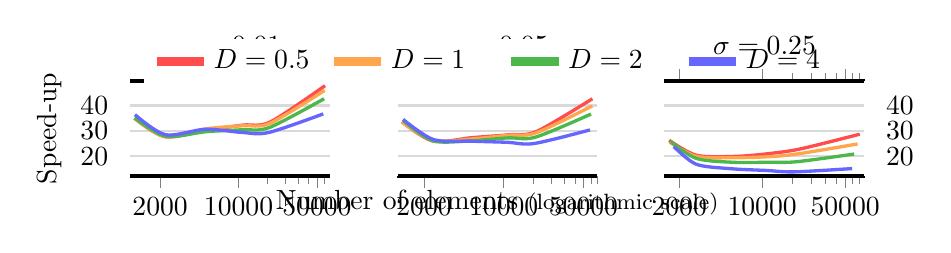
\begin{tikzpicture}
\begin{scope}[shift={(0.0\linewidth,0)}]
\begin{axis}[
 width=0.34\linewidth,height=0.23\linewidth,
 title=\normalsize\mbox{$\sigma=0.01$},
 xmode=log,enlarge x limits=0.025,
 ylabel=Speed-up,
 axis y line*=left,
 ymin=12.0793620886,ymax=49.6291431477,
 tick align=outside,
 x axis line style = ultra thick,y axis line style={white},
 xtick={2000,10000,50000},xticklabels={2000,10000,50000},
 minor xtick={18000,26000,34000,42000,58000,66000}, every y tick/.style={white},ymajorgrids,grid style={gray!30,thick}]
\addplot[very thick,mark=none,smooth,color=red!70] table[] {
	1181.62066667 34.9247874428
	2215.46 27.6488159311
	5181.616 30.264035458
	10893.6296667 32.2484055952
	19119.5003333 33.4710920118
	59054.826 47.8410583353
};
\addplot[very thick,mark=none,smooth,color=orange!70] table[] {
	1181.62066667 34.9934469201
	2217.06433333 27.6413774549
	5155.626 30.7970360825
	10845.362 32.0099478668
	18986.0146667 32.9400119976
	58578.4676667 45.9683063494
};
\addplot[very thick,mark=none,smooth,color=green!60!black!70] table[] {
	1184.32666667 35.1084812623
	2229.279 27.8587310195
	5150.313 29.6630119983
	10787.995 30.4238547881
	18838.031 31.3061573546
	57902.6766667 42.6751507093
};
\addplot[very thick,mark=none,smooth,color=blue!60!] table[] {
	1191.78133333 36.3760217984
	2227.87566667 28.4449058693
	5053.76633333 30.6260145237
	10584.265 29.3838753785
	18489.5223333 29.3124432819
	56902.9196667 36.6790190189
};
!\end{axis}
\end{scope}
\begin{scope}[shift={(0.28\linewidth,0)}]
\begin{axis}[
 width=0.34\linewidth,height=0.23\linewidth,
 title=\normalsize\mbox{$\sigma=0.05$},
 xmode=log,enlarge x limits=0.025,
 xlabel=Number of elements \footnotesize(logarithmic scale),x label style={at={(axis description cs:0.5,-0.05)},anchor=north},
 yticklabels={},
 legend style={at={(0.55,1.45)},legend style={text width=4em},legend style={draw=none},anchor=north,legend columns=-1},
 axis y line*=left,
 ymin=12.0793620886,ymax=49.6291431477,
 tick align=outside,
 x axis line style = ultra thick,y axis line style={white},
 xtick={2000,10000,50000},xticklabels={2000,10000,50000},
 minor xtick={18000,26000,34000,42000,58000,66000}, every y tick/.style={white},ymajorgrids,grid style={gray!30,thick}]
\addlegendimage{line width=3pt,mark=none,red!70}
\addlegendentry{$D=0.5$}
\addlegendimage{line width=3pt,mark=none,orange!70}
\addlegendentry{$D=1$}
\addlegendimage{line width=3pt,mark=none,green!60!black!70}
\addlegendentry{$D=2$}
\addlegendimage{line width=3pt,mark=none,blue!60!}
\addlegendentry{$D=4$}
\addplot[very thick,mark=none,smooth,color=red!70] table[] {
	1279.641 33.5481434865
	2390.32533333 25.94882189
	5290.78533333 27.3147946561
	11085.4573333 28.4281185456
	19376.218 29.738855758
	59892.9113333 42.6625314879
};
\addplot[very thick,mark=none,smooth,color=orange!70] table[] {
	1278.69166667 33.4639045825
	2410.959 26.1275510204
	5292.737 26.8002718711
	11011.373 28.2517065254
	19272.0743333 29.2044390961
	59537.7083333 39.8134020879
};
\addplot[very thick,mark=none,smooth,color=green!60!black!70] table[] {
	1316.78633333 34.0408684547
	2403.786 26.0279542567
	5295.75033333 26.0884688091
	10928.2076667 27.2050103425
	18998.6893333 27.4921961535
	58278.8796667 36.6218746609
};
\addplot[very thick,mark=none,smooth,color=blue!60!] table[] {
	1310.299 34.5035598706
	2415.94733333 26.5543168265
	5160.93433333 25.9121291776
	10652.052 25.4688441346
	18520.5773333 24.9919904801
	56986.4536667 30.3469638098
};
!\end{axis}
\end{scope}
\begin{scope}[shift={(0.56\linewidth,0)}]
\begin{axis}[
 width=0.34\linewidth,height=0.23\linewidth,
 title=\normalsize\mbox{$\sigma=0.25$},
 xmode=log,enlarge x limits=0.025,
 axis y line*=right,
 ymin=12.0793620886,ymax=49.6291431477,
 tick align=outside,
 x axis line style = ultra thick,y axis line style={white},
 xtick={2000,10000,50000},xticklabels={2000,10000,50000},
 minor xtick={18000,26000,34000,42000,58000,66000}, every y tick/.style={white},ymajorgrids,grid style={gray!30,thick}]
\addplot[very thick,mark=none,smooth,color=red!70] table[] {
	1646.15933333 26.2552773687
	2810.362 20.3094430026
	6177.13333333 19.9247177833
	12514.3133333 21.2175424619
	21685.3016667 22.9935564818
	66406.0556667 28.6586405206
};
\addplot[very thick,mark=none,smooth,color=orange!70] table[] {
	1663.08533333 25.516221374
	2790.36366667 19.8924520923
	5894.47266667 19.3723184377
	11932.3566667 19.8233801387
	20686.2586667 20.9873832955
	63703.007 24.8033266758
};
\addplot[very thick,mark=none,smooth,color=green!60!black!70] table[] {
	1688.79933333 25.7868852459
	2772.61566667 19.1257755217
	5654.935 17.5703296703
	11315.806 17.5734125199
	19524.696 17.7848707152
	59597.5723333 20.8215000155
};
\addplot[very thick,mark=none,smooth,color=blue!60!] table[] {
	1801.26033333 23.7592181253
	2773.10966667 16.8232181247
	5387.17566667 15.0388956512
	10819.9246667 14.3352091999
	18649.48 13.7823000051
	57325.7383333 15.0790955552
};
!\end{axis}
\end{scope}
\end{tikzpicture}
\end{center}
\caption{Speed-up results by mesh remodelling - Boeing 737 airfoil}\centering\sffamily\footnotesize
Average of thirty optimisation scenarios\end{figure}

\pagebreak
\subsubsection{RAE 2822}
\vspace*{\fill} \begin{table}[!hp]
\begin{center}
\begin{tabular}{c|cc?c|c?c?c|c|c||c|c}
\multirow{2}{*}{\textbf{\large $\boldsymbol{\sigma}$}} & \multirow{2}{*}{\textbf{\large $\boldsymbol{I}$}} & \multirow{2}{*}{\textbf{\large $\boldsymbol{G}$}} & \multicolumn{2}{c?}{\textbf{\large Generation}} & \multirow{2}{*}{\textbf{\large $\boldsymbol{D}$}} & \multicolumn{5}{c}{\textbf{{\large Remodelling} }} \\\cline{4-5}\cline{7-11}
 & & & \textbf{\# Tri.} & \textbf{Time} & &\textbf{\# Tri.} & \textbf{Time} & \textbf{Preserv.} & \textbf{+ Tri.} & \textbf{Sp.-up} \\\toprule
\multirow{24}[11]{*}{.01} & \multirow{4}{*}{50} & \multirow{4}{*}{1} & \multirow{4}{*}{1231} & \multirow{4}{*}{1.87 ms} & .5 & 1143 & 0.05 ms & 90.62 \% & -7.19 \% & 36.29 \\\cline{6-11}
 & & & &  & 1 & 1143 & 0.05 ms & 90.62 \% & -7.19 \% & 36.29 \\\cline{6-11}
 & & & &  & 2 & 1147 & 0.05 ms & 90.65 \% & -6.81 \% & 36.17 \\\cline{6-11}
 & & & &  & 4 & 1149 & 0.05 ms & 90.82 \% & -6.72 \% & 38.17 \\\cmidrule[1.5pt]{2-11}
 & \multirow{4}{*}{100} & \multirow{4}{*}{2} & \multirow{4}{*}{1856} & \multirow{4}{*}{3.47 ms} & .5 & 2190 & 0.12 ms & 89.93 \% & 18.03 \% & 28.77 \\\cline{6-11}
 & & & &  & 1 & 2204 & 0.12 ms & 89.98 \% & 18.76 \% & 28.60 \\\cline{6-11}
 & & & &  & 2 & 2198 & 0.12 ms & 89.99 \% & 18.44 \% & 29.39 \\\cline{6-11}
 & & & &  & 4 & 2180 & 0.12 ms & 90.00 \% & 17.46 \% & 29.83 \\\cmidrule[1.5pt]{2-11}
 & \multirow{4}{*}{200} & \multirow{4}{*}{4} & \multirow{4}{*}{4656} & \multirow{4}{*}{9.76 ms} & .5 & 5024 & 0.29 ms & 91.23 \% & 7.90 \% & 33.61 \\\cline{6-11}
 & & & &  & 1 & 5020 & 0.29 ms & 91.24 \% & 7.81 \% & 33.61 \\\cline{6-11}
 & & & &  & 2 & 5049 & 0.29 ms & 91.28 \% & 8.43 \% & 33.47 \\\cline{6-11}
 & & & &  & 4 & 4988 & 0.30 ms & 91.24 \% & 7.13 \% & 33.04 \\\cmidrule[1.5pt]{2-11}
 & \multirow{4}{*}{300} & \multirow{4}{*}{6} & \multirow{4}{*}{9904} & \multirow{4}{*}{20.91 ms} & .5 & 10557 & 0.54 ms & 93.56 \% & 6.59 \% & 38.76 \\\cline{6-11}
 & & & &  & 1 & 10559 & 0.54 ms & 93.57 \% & 6.61 \% & 39.04 \\\cline{6-11}
 & & & &  & 2 & 10575 & 0.56 ms & 93.55 \% & 6.77 \% & 37.53 \\\cline{6-11}
 & & & &  & 4 & 10445 & 0.58 ms & 93.44 \% & 5.46 \% & 36.24 \\\cmidrule[1.5pt]{2-11}
 & \multirow{4}{*}{400} & \multirow{4}{*}{8} & \multirow{4}{*}{17522} & \multirow{4}{*}{37.35 ms} & .5 & 18518 & 0.91 ms & 94.95 \% & 5.69 \% & 41.25 \\\cline{6-11}
 & & & &  & 1 & 18496 & 0.89 ms & 94.93 \% & 5.56 \% & 41.78 \\\cline{6-11}
 & & & &  & 2 & 18463 & 0.95 ms & 94.89 \% & 5.37 \% & 39.32 \\\cline{6-11}
 & & & &  & 4 & 18253 & 1.03 ms & 94.75 \% & 4.18 \% & 36.39 \\\cmidrule[1.5pt]{2-11}
 & \multirow{4}{*}{700} & \multirow{4}{*}{14} & \multirow{4}{*}{54517} & \multirow{4}{*}{161.17 ms} & .5 & 57160 & 2.54 ms & 96.89 \% & 4.85 \% & 63.50 \\\cline{6-11}
 & & & &  & 1 & 56994 & 2.62 ms & 96.87 \% & 4.54 \% & 61.50 \\\cline{6-11}
 & & & &  & 2 & 56796 & 2.88 ms & 96.77 \% & 4.18 \% & 55.86 \\\cline{6-11}
 & & & &  & 4 & 56235 & 3.42 ms & 96.59 \% & 3.15 \% & 47.12\\\bottomrule
\end{tabular}\end{center}
\caption{Full results of mesh remodelling for $\sigma=0.01$ - RAE 2822 airfoil}\centering\sffamily\footnotesize
Average of thirty optimisation scenarios\end{table}
 \vspace*{\fill}
\begin{table}[!hp]
\begin{center}
\begin{tabular}{c|cc?c|c?c?c|c|c||c|c}
\multirow{2}{*}{\textbf{\large $\boldsymbol{\sigma}$}} & \multirow{2}{*}{\textbf{\large $\boldsymbol{I}$}} & \multirow{2}{*}{\textbf{\large $\boldsymbol{G}$}} & \multicolumn{2}{c?}{\textbf{\large Generation}} & \multirow{2}{*}{\textbf{\large $\boldsymbol{D}$}} & \multicolumn{5}{c}{\textbf{{\large Remodelling} }} \\\cline{4-5}\cline{7-11}
 & & & \textbf{\# Tri.} & \textbf{Time} & &\textbf{\# Tri.} & \textbf{Time} & \textbf{Preserv.} & \textbf{+ Tri.} & \textbf{Sp.-up} \\\toprule
\multirow{24}[13]{*}{.05} & \multirow{4}{*}{50} & \multirow{4}{*}{1} & \multirow{4}{*}{1224} & \multirow{4}{*}{1.86 ms} & .5 & 1298 & 0.05 ms & 91.49 \% & 6.06 \% & 34.92 \\\cline{6-11}
 & & & &  & 1 & 1298 & 0.05 ms & 91.50 \% & 6.02 \% & 34.90 \\\cline{6-11}
 & & & &  & 2 & 1303 & 0.05 ms & 91.53 \% & 6.45 \% & 35.43 \\\cline{6-11}
 & & & &  & 4 & 1300 & 0.05 ms & 91.61 \% & 6.19 \% & 36.15 \\\cmidrule[1.5pt]{2-11}
 & \multirow{4}{*}{100} & \multirow{4}{*}{2} & \multirow{4}{*}{1852} & \multirow{4}{*}{3.46 ms} & .5 & 2341 & 0.13 ms & 90.46 \% & 26.41 \% & 27.25 \\\cline{6-11}
 & & & &  & 1 & 2350 & 0.13 ms & 90.48 \% & 26.91 \% & 26.92 \\\cline{6-11}
 & & & &  & 2 & 2350 & 0.13 ms & 90.48 \% & 26.89 \% & 27.13 \\\cline{6-11}
 & & & &  & 4 & 2328 & 0.13 ms & 90.51 \% & 25.71 \% & 27.46 \\\cmidrule[1.5pt]{2-11}
 & \multirow{4}{*}{200} & \multirow{4}{*}{4} & \multirow{4}{*}{4659} & \multirow{4}{*}{9.60 ms} & .5 & 5187 & 0.32 ms & 91.39 \% & 11.34 \% & 30.25 \\\cline{6-11}
 & & & &  & 1 & 5212 & 0.32 ms & 91.42 \% & 11.87 \% & 30.00 \\\cline{6-11}
 & & & &  & 2 & 5219 & 0.33 ms & 91.41 \% & 12.03 \% & 29.47 \\\cline{6-11}
 & & & &  & 4 & 5087 & 0.34 ms & 91.22 \% & 9.20 \% & 28.55 \\\cmidrule[1.5pt]{2-11}
 & \multirow{4}{*}{300} & \multirow{4}{*}{6} & \multirow{4}{*}{9904} & \multirow{4}{*}{20.25 ms} & .5 & 10853 & 0.60 ms & 93.60 \% & 9.58 \% & 34.00 \\\cline{6-11}
 & & & &  & 1 & 10822 & 0.61 ms & 93.58 \% & 9.27 \% & 33.44 \\\cline{6-11}
 & & & &  & 2 & 10752 & 0.63 ms & 93.51 \% & 8.56 \% & 31.92 \\\cline{6-11}
 & & & &  & 4 & 10537 & 0.69 ms & 93.27 \% & 6.38 \% & 29.37 \\\cmidrule[1.5pt]{2-11}
 & \multirow{4}{*}{400} & \multirow{4}{*}{8} & \multirow{4}{*}{17522} & \multirow{4}{*}{37.31 ms} & .5 & 18944 & 1.00 ms & 94.93 \% & 8.11 \% & 37.48 \\\cline{6-11}
 & & & &  & 1 & 18923 & 1.04 ms & 94.90 \% & 7.99 \% & 35.82 \\\cline{6-11}
 & & & &  & 2 & 18722 & 1.11 ms & 94.79 \% & 6.84 \% & 33.71 \\\cline{6-11}
 & & & &  & 4 & 18361 & 1.23 ms & 94.55 \% & 4.79 \% & 30.36 \\\cmidrule[1.5pt]{2-11}
 & \multirow{4}{*}{700} & \multirow{4}{*}{14} & \multirow{4}{*}{54516} & \multirow{4}{*}{160.95 ms} & .5 & 58605 & 2.92 ms & 96.83 \% & 7.50 \% & 55.16 \\\cline{6-11}
 & & & &  & 1 & 58453 & 3.12 ms & 96.77 \% & 7.22 \% & 51.51 \\\cline{6-11}
 & & & &  & 2 & 57464 & 3.48 ms & 96.65 \% & 5.41 \% & 46.29 \\\cline{6-11}
 & & & &  & 4 & 56479 & 4.26 ms & 96.37 \% & 3.60 \% & 37.75\\\bottomrule
\end{tabular}\end{center}
\caption{Full results of mesh remodelling for $\sigma=0.05$ - RAE 2822 airfoil}\centering\sffamily\footnotesize
Average of thirty optimisation scenarios\end{table}

\begin{table}[!hp]
\begin{center}
\begin{tabular}{c|cc?c|c?c?c|c|c||c|c}
\multirow{2}{*}{\textbf{\large $\boldsymbol{\sigma}$}} & \multirow{2}{*}{\textbf{\large $\boldsymbol{I}$}} & \multirow{2}{*}{\textbf{\large $\boldsymbol{G}$}} & \multicolumn{2}{c?}{\textbf{\large Generation}} & \multirow{2}{*}{\textbf{\large $\boldsymbol{D}$}} & \multicolumn{5}{c}{\textbf{{\large Remodelling} }} \\\cline{4-5}\cline{7-11}
 & & & \textbf{\# Tri.} & \textbf{Time} & &\textbf{\# Tri.} & \textbf{Time} & \textbf{Preserv.} & \textbf{+ Tri.} & \textbf{Sp.-up} \\\toprule
\multirow{24}[13]{*}{.25} & \multirow{4}{*}{50} & \multirow{4}{*}{1} & \multirow{4}{*}{1214} & \multirow{4}{*}{1.84 ms} & .5 & 1596 & 0.07 ms & 92.69 \% & 31.53 \% & 27.27 \\\cline{6-11}
 & & & &  & 1 & 1608 & 0.07 ms & 92.79 \% & 32.47 \% & 27.14 \\\cline{6-11}
 & & & &  & 2 & 1657 & 0.07 ms & 92.88 \% & 36.52 \% & 26.39 \\\cline{6-11}
 & & & &  & 4 & 1715 & 0.07 ms & 93.15 \% & 41.31 \% & 24.72 \\\cmidrule[1.5pt]{2-11}
 & \multirow{4}{*}{100} & \multirow{4}{*}{2} & \multirow{4}{*}{1854} & \multirow{4}{*}{3.42 ms} & .5 & 2757 & 0.17 ms & 91.56 \% & 48.72 \% & 20.33 \\\cline{6-11}
 & & & &  & 1 & 2758 & 0.17 ms & 91.51 \% & 48.77 \% & 19.90 \\\cline{6-11}
 & & & &  & 2 & 2746 & 0.18 ms & 91.40 \% & 48.17 \% & 19.02 \\\cline{6-11}
 & & & &  & 4 & 2716 & 0.20 ms & 91.09 \% & 46.55 \% & 17.06 \\\cmidrule[1.5pt]{2-11}
 & \multirow{4}{*}{200} & \multirow{4}{*}{4} & \multirow{4}{*}{4656} & \multirow{4}{*}{9.14 ms} & .5 & 6060 & 0.44 ms & 92.17 \% & 30.16 \% & 20.56 \\\cline{6-11}
 & & & &  & 1 & 5836 & 0.46 ms & 91.78 \% & 25.35 \% & 19.71 \\\cline{6-11}
 & & & &  & 2 & 5559 & 0.51 ms & 91.14 \% & 19.40 \% & 17.92 \\\cline{6-11}
 & & & &  & 4 & 5316 & 0.61 ms & 90.33 \% & 14.18 \% & 15.04 \\\cmidrule[1.5pt]{2-11}
 & \multirow{4}{*}{300} & \multirow{4}{*}{6} & \multirow{4}{*}{9895} & \multirow{4}{*}{19.76 ms} & .5 & 12338 & 0.90 ms & 93.89 \% & 24.70 \% & 21.85 \\\cline{6-11}
 & & & &  & 1 & 11813 & 0.96 ms & 93.51 \% & 19.39 \% & 20.63 \\\cline{6-11}
 & & & &  & 2 & 11210 & 1.09 ms & 92.90 \% & 13.29 \% & 18.11 \\\cline{6-11}
 & & & &  & 4 & 10719 & 1.36 ms & 92.00 \% & 8.33 \% & 14.58 \\\cmidrule[1.5pt]{2-11}
 & \multirow{4}{*}{400} & \multirow{4}{*}{8} & \multirow{4}{*}{17501} & \multirow{4}{*}{36.46 ms} & .5 & 21384 & 1.49 ms & 95.01 \% & 22.19 \% & 24.53 \\\cline{6-11}
 & & & &  & 1 & 20455 & 1.65 ms & 94.64 \% & 16.88 \% & 22.08 \\\cline{6-11}
 & & & &  & 2 & 19330 & 1.99 ms & 94.04 \% & 10.46 \% & 18.31 \\\cline{6-11}
 & & & &  & 4 & 18519 & 2.58 ms & 93.12 \% & 5.82 \% & 14.14 \\\cmidrule[1.5pt]{2-11}
 & \multirow{4}{*}{700} & \multirow{4}{*}{14} & \multirow{4}{*}{54443} & \multirow{4}{*}{158.33 ms} & .5 & 65427 & 5.23 ms & 96.64 \% & 20.18 \% & 30.28 \\\cline{6-11}
 & & & &  & 1 & 63005 & 6.08 ms & 96.32 \% & 15.73 \% & 26.03 \\\cline{6-11}
 & & & &  & 2 & 59103 & 7.36 ms & 95.77 \% & 8.56 \% & 21.52 \\\cline{6-11}
 & & & &  & 4 & 56886 & 10.33 ms & 94.82 \% & 4.49 \% & 15.33\\\bottomrule
\end{tabular}\end{center}
\caption{Full results of mesh remodelling for $\sigma=0.25$ - RAE 2822 airfoil}\centering\sffamily\footnotesize
Average of thirty optimisation scenarios\end{table}
 \newpage
\begin{figure}[!h]
\begin{center}
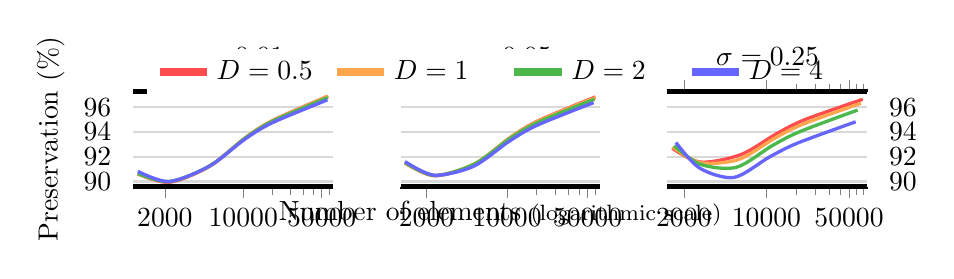
\begin{tikzpicture}
\begin{scope}[shift={(0.0\linewidth,0)}]
\begin{axis}[
 width=0.34\linewidth,height=0.23\linewidth,
 title=\normalsize\mbox{$\sigma=0.01$},
 xmode=log,enlarge x limits=0.025,
 ylabel=Preservation (\%),
 axis y line*=left,
 ymin=89.5852833333,ymax=97.2597858333,
 tick align=outside,
 x axis line style = ultra thick,y axis line style={white},
 xtick={2000,10000,50000},xticklabels={2000,10000,50000},
 minor xtick={18000,26000,34000,42000,58000,66000}, every y tick/.style={white},ymajorgrids,grid style={gray!30,thick}]
\addplot[very thick,mark=none,smooth,color=red!70] table[] {
	1142.66433333 90.6223333333
	2190.331 89.9333333333
	5024.068 91.2336666667
	10557.4073333 93.559
	18518.477 94.946
	57160.1013333 96.8943333333
};
\addplot[very thick,mark=none,smooth,color=orange!70] table[] {
	1142.66433333 90.6223333333
	2203.91966667 89.983
	5019.90933333 91.2416666667
	10559.26 93.5726666667
	18496.2383333 94.9303333333
	56994.2803333 96.8676666667
};
\addplot[very thick,mark=none,smooth,color=green!60!black!70] table[] {
	1147.421 90.6463333333
	2198.01033333 89.9903333333
	5048.57 91.277
	10575.013 93.5463333333
	18463.3696667 94.888
	56796.2563333 96.7726666667
};
\addplot[very thick,mark=none,smooth,color=blue!60!] table[] {
	1148.51366667 90.8193333333
	2179.72533333 89.9976666667
	4988.35566667 91.237
	10445.26 93.4446666667
	18253.313 94.7536666667
	56234.555 96.5863333333
};
!\end{axis}
\end{scope}
\begin{scope}[shift={(0.28\linewidth,0)}]
\begin{axis}[
 width=0.34\linewidth,height=0.23\linewidth,
 title=\normalsize\mbox{$\sigma=0.05$},
 xmode=log,enlarge x limits=0.025,
 xlabel=Number of elements \footnotesize(logarithmic scale),x label style={at={(axis description cs:0.5,-0.05)},anchor=north},
 yticklabels={},
 legend style={at={(0.55,1.45)},legend style={text width=4em},legend style={draw=none},anchor=north,legend columns=-1},
 axis y line*=left,
 ymin=89.5852833333,ymax=97.2597858333,
 tick align=outside,
 x axis line style = ultra thick,y axis line style={white},
 xtick={2000,10000,50000},xticklabels={2000,10000,50000},
 minor xtick={18000,26000,34000,42000,58000,66000}, every y tick/.style={white},ymajorgrids,grid style={gray!30,thick}]
\addlegendimage{line width=3pt,mark=none,red!70}
\addlegendentry{$D=0.5$}
\addlegendimage{line width=3pt,mark=none,orange!70}
\addlegendentry{$D=1$}
\addlegendimage{line width=3pt,mark=none,green!60!black!70}
\addlegendentry{$D=2$}
\addlegendimage{line width=3pt,mark=none,blue!60!}
\addlegendentry{$D=4$}
\addplot[very thick,mark=none,smooth,color=red!70] table[] {
	1298.20533333 91.495
	2340.633 90.4603333333
	5186.95033333 91.389
	10853.1023333 93.6036666667
	18943.9993333 94.9333333333
	58604.5323333 96.8286666667
};
\addplot[very thick,mark=none,smooth,color=orange!70] table[] {
	1297.63266667 91.496
	2349.96633333 90.4843333333
	5211.535 91.4193333333
	10822.068 93.583
	18923.0946667 94.8986666667
	58453.4236667 96.7666666667
};
\addplot[very thick,mark=none,smooth,color=green!60!black!70] table[] {
	1302.89433333 91.533
	2349.60333333 90.4793333333
	5219.07066667 91.411
	10751.7493333 93.5096666667
	18721.5463333 94.7916666667
	57464.189 96.6476666667
};
\addplot[very thick,mark=none,smooth,color=blue!60!] table[] {
	1299.731 91.6113333333
	2327.66833333 90.506
	5087.395 91.215
	10536.52 93.2713333333
	18361.0733333 94.5533333333
	56479.5 96.3676666667
};
!\end{axis}
\end{scope}
\begin{scope}[shift={(0.56\linewidth,0)}]
\begin{axis}[
 width=0.34\linewidth,height=0.23\linewidth,
 title=\normalsize\mbox{$\sigma=0.25$},
 xmode=log,enlarge x limits=0.025,
 axis y line*=right,
 ymin=89.5852833333,ymax=97.2597858333,
 tick align=outside,
 x axis line style = ultra thick,y axis line style={white},
 xtick={2000,10000,50000},xticklabels={2000,10000,50000},
 minor xtick={18000,26000,34000,42000,58000,66000}, every y tick/.style={white},ymajorgrids,grid style={gray!30,thick}]
\addplot[very thick,mark=none,smooth,color=red!70] table[] {
	1596.30333333 92.689
	2756.53766667 91.5646666667
	6060.21733333 92.1663333333
	12338.161 93.8876666667
	21383.8163333 95.011
	65427.1206667 96.6373333333
};
\addplot[very thick,mark=none,smooth,color=orange!70] table[] {
	1607.67666667 92.7946666667
	2757.58366667 91.5123333333
	5836.15333333 91.7793333333
	11813.4666667 93.507
	20455.343 94.6356666667
	63005.4993333 96.319
};
\addplot[very thick,mark=none,smooth,color=green!60!black!70] table[] {
	1656.74966667 92.8756666667
	2746.29366667 91.396
	5559.30066667 91.1436666667
	11210.0 92.8956666667
	19330.474 94.0383333333
	59102.68 95.7656666667
};
\addplot[very thick,mark=none,smooth,color=blue!60!] table[] {
	1714.92766667 93.146
	2716.32133333 91.086
	5316.24133333 90.3253333333
	10718.991 92.003
	18519.036 93.117
	56886.458 94.8183333333
};
!\end{axis}
\end{scope}
\end{tikzpicture}
\end{center}
\caption{Element preservation results using mesh remodelling - RAE 2822 airfoil}\centering\sffamily\footnotesize
Average of thirty optimisation scenarios\end{figure}

\begin{figure}[!h]
\begin{center}
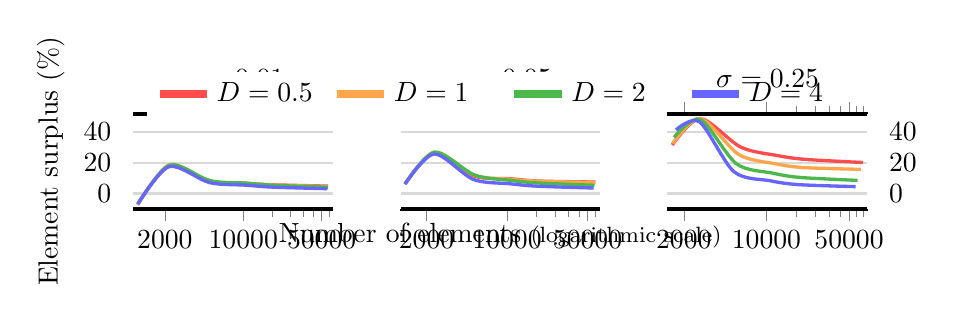
\begin{tikzpicture}
\begin{scope}[shift={(0.0\linewidth,0)}]
\begin{axis}[
 width=0.34\linewidth,height=0.23\linewidth,
 title=\normalsize\mbox{$\sigma=0.01$},
 xmode=log,enlarge x limits=0.025,
 ylabel=Element surplus (\%),
 axis y line*=left,
 ymin=-9.99254435348,ymax=51.7132290624,
 tick align=outside,
 x axis line style = ultra thick,y axis line style={white},
 xtick={2000,10000,50000},xticklabels={2000,10000,50000},
 minor xtick={18000,26000,34000,42000,58000,66000}, every y tick/.style={white},ymajorgrids,grid style={gray!30,thick}]
\addplot[very thick,mark=none,smooth,color=red!70] table[] {
	1142.66433333 -7.19409657952
	2190.331 18.0292948627
	5024.068 7.89971733263
	10557.4073333 6.5949868196
	18518.477 5.68929699423
	57160.1013333 4.84824826573
};
\addplot[very thick,mark=none,smooth,color=orange!70] table[] {
	1142.66433333 -7.19409657952
	2203.91966667 18.7615406944
	5019.90933333 7.81040346231
	10559.26 6.61369264127
	18496.2383333 5.56237570118
	56994.2803333 4.54408433022
};
\addplot[very thick,mark=none,smooth,color=green!60!black!70] table[] {
	1147.421 -6.80776549839
	2198.01033333 18.4431073405
	5048.57 8.42593610078
	10575.013 6.77274597457
	18463.3696667 5.37478650186
	56796.2563333 4.18085072793
};
\addplot[very thick,mark=none,smooth,color=blue!60!] table[] {
	1148.51366667 -6.71902034885
	2179.72533333 17.4577924924
	4988.35566667 7.13273912454
	10445.26 5.46266870957
	18253.313 4.17594377689
	56234.555 3.15052713727
};
!\end{axis}
\end{scope}
\begin{scope}[shift={(0.28\linewidth,0)}]
\begin{axis}[
 width=0.34\linewidth,height=0.23\linewidth,
 title=\normalsize\mbox{$\sigma=0.05$},
 xmode=log,enlarge x limits=0.025,
 xlabel=Number of elements \footnotesize(logarithmic scale),x label style={at={(axis description cs:0.5,-0.05)},anchor=north},
 yticklabels={},
 legend style={at={(0.55,1.45)},legend style={text width=4em},legend style={draw=none},anchor=north,legend columns=-1},
 axis y line*=left,
 ymin=-9.99254435348,ymax=51.7132290624,
 tick align=outside,
 x axis line style = ultra thick,y axis line style={white},
 xtick={2000,10000,50000},xticklabels={2000,10000,50000},
 minor xtick={18000,26000,34000,42000,58000,66000}, every y tick/.style={white},ymajorgrids,grid style={gray!30,thick}]
\addlegendimage{line width=3pt,mark=none,red!70}
\addlegendentry{$D=0.5$}
\addlegendimage{line width=3pt,mark=none,orange!70}
\addlegendentry{$D=1$}
\addlegendimage{line width=3pt,mark=none,green!60!black!70}
\addlegendentry{$D=2$}
\addlegendimage{line width=3pt,mark=none,blue!60!}
\addlegendentry{$D=4$}
\addplot[very thick,mark=none,smooth,color=red!70] table[] {
	1298.20533333 6.06322045678
	2340.633 26.4079832236
	5186.95033333 11.3377964278
	10853.1023333 9.57867583198
	18943.9993333 8.11295780414
	58604.5323333 7.50044176941
};
\addplot[very thick,mark=none,smooth,color=orange!70] table[] {
	1297.63266667 6.01643365861
	2349.96633333 26.9120382563
	5211.535 11.8655058595
	10822.068 9.26533674722
	18923.0946667 7.99365536406
	58453.4236667 7.22325760336
};
\addplot[very thick,mark=none,smooth,color=green!60!black!70] table[] {
	1302.89433333 6.44631119593
	2349.60333333 26.892434116
	5219.07066667 12.0272588102
	10751.7493333 8.55536220326
	18721.5463333 6.84342377496
	57464.189 5.40866819455
};
\addplot[very thick,mark=none,smooth,color=blue!60!] table[] {
	1299.731 6.18786724096
	2327.66833333 25.7078147792
	5087.395 9.20084297278
	10536.52 6.3822927322
	18361.0733333 4.78621285805
	56479.5 3.60241706872
};
!\end{axis}
\end{scope}
\begin{scope}[shift={(0.56\linewidth,0)}]
\begin{axis}[
 width=0.34\linewidth,height=0.23\linewidth,
 title=\normalsize\mbox{$\sigma=0.25$},
 xmode=log,enlarge x limits=0.025,
 axis y line*=right,
 ymin=-9.99254435348,ymax=51.7132290624,
 tick align=outside,
 x axis line style = ultra thick,y axis line style={white},
 xtick={2000,10000,50000},xticklabels={2000,10000,50000},
 minor xtick={18000,26000,34000,42000,58000,66000}, every y tick/.style={white},ymajorgrids,grid style={gray!30,thick}]
\addplot[very thick,mark=none,smooth,color=red!70] table[] {
	1596.30333333 31.5342999505
	2756.53766667 48.7184259783
	6060.21733333 30.1597822272
	12338.161 24.6954469507
	21383.8163333 22.1880437805
	65427.1206667 20.1757517151
};
\addplot[very thick,mark=none,smooth,color=orange!70] table[] {
	1607.67666667 32.4714548176
	2757.58366667 48.7748588997
	5836.15333333 25.3473935221
	11813.4666667 19.3926312064
	20455.343 16.8827073272
	63005.4993333 15.7277466503
};
\addplot[very thick,mark=none,smooth,color=green!60!black!70] table[] {
	1656.74966667 36.5150363642
	2746.29366667 48.1657502162
	5559.30066667 19.4012234724
	11210.0 13.2937040064
	19330.474 10.4551576103
	59102.68 8.55909483723
};
\addplot[very thick,mark=none,smooth,color=blue!60!] table[] {
	1714.92766667 41.3088636668
	2716.32133333 46.5487078336
	5316.24133333 14.1808579055
	10718.991 8.33132859961
	18519.036 5.81856607198
	56886.458 4.48836480809
};
!\end{axis}
\end{scope}
\end{tikzpicture}
\end{center}
\caption{Element surplus results on meshes from mesh remodelling - RAE 2822 airfoil}\centering\sffamily\footnotesize
Average of thirty optimisation scenarios\end{figure}

\input{Appendix/figures/plots/rae2822_su}
\pagebreak
\subsubsection{NACA 63206}
\vspace*{\fill} \begin{table}[!hp]
\begin{center}
\begin{tabular}{c|cc?c|c?c?c|c|c||c|c}
\multirow{2}{*}{\textbf{\large $\boldsymbol{\sigma}$}} & \multirow{2}{*}{\textbf{\large $\boldsymbol{I}$}} & \multirow{2}{*}{\textbf{\large $\boldsymbol{G}$}} & \multicolumn{2}{c?}{\textbf{\large Generation}} & \multirow{2}{*}{\textbf{\large $\boldsymbol{D}$}} & \multicolumn{5}{c}{\textbf{{\large Remodelling} }} \\\cline{4-5}\cline{7-11}
 & & & \textbf{\# Tri.} & \textbf{Time} & &\textbf{\# Tri.} & \textbf{Time} & \textbf{Preserv.} & \textbf{+ Tri.} & \textbf{Sp.-up} \\\toprule
\multirow{24}[11]{*}{.01} & \multirow{4}{*}{50} & \multirow{4}{*}{1} & \multirow{4}{*}{1218} & \multirow{4}{*}{1.89 ms} & .5 & 1340 & 0.05 ms & 91.71 \% & 10.01 \% & 34.31 \\\cline{6-11}
 & & & &  & 1 & 1340 & 0.06 ms & 91.71 \% & 10.01 \% & 34.25 \\\cline{6-11}
 & & & &  & 2 & 1353 & 0.05 ms & 91.77 \% & 11.12 \% & 34.46 \\\cline{6-11}
 & & & &  & 4 & 1350 & 0.05 ms & 91.81 \% & 10.89 \% & 34.35 \\\cmidrule[1.5pt]{2-11}
 & \multirow{4}{*}{100} & \multirow{4}{*}{2} & \multirow{4}{*}{1913} & \multirow{4}{*}{3.53 ms} & .5 & 2421 & 0.14 ms & 90.63 \% & 26.54 \% & 26.01 \\\cline{6-11}
 & & & &  & 1 & 2437 & 0.14 ms & 90.68 \% & 27.39 \% & 25.98 \\\cline{6-11}
 & & & &  & 2 & 2476 & 0.14 ms & 90.84 \% & 29.42 \% & 25.97 \\\cline{6-11}
 & & & &  & 4 & 2465 & 0.14 ms & 90.86 \% & 28.85 \% & 25.64 \\\cmidrule[1.5pt]{2-11}
 & \multirow{4}{*}{200} & \multirow{4}{*}{4} & \multirow{4}{*}{4824} & \multirow{4}{*}{9.46 ms} & .5 & 5621 & 0.34 ms & 91.96 \% & 16.52 \% & 28.13 \\\cline{6-11}
 & & & &  & 1 & 5562 & 0.34 ms & 91.87 \% & 15.31 \% & 28.06 \\\cline{6-11}
 & & & &  & 2 & 5481 & 0.35 ms & 91.70 \% & 13.62 \% & 26.69 \\\cline{6-11}
 & & & &  & 4 & 5298 & 0.37 ms & 91.38 \% & 9.83 \% & 25.46 \\\cmidrule[1.5pt]{2-11}
 & \multirow{4}{*}{300} & \multirow{4}{*}{6} & \multirow{4}{*}{10184} & \multirow{4}{*}{20.50 ms} & .5 & 11779 & 0.65 ms & 94.03 \% & 15.66 \% & 31.56 \\\cline{6-11}
 & & & &  & 1 & 11592 & 0.66 ms & 93.92 \% & 13.83 \% & 31.25 \\\cline{6-11}
 & & & &  & 2 & 11371 & 0.70 ms & 93.72 \% & 11.66 \% & 29.46 \\\cline{6-11}
 & & & &  & 4 & 10943 & 0.77 ms & 93.33 \% & 7.45 \% & 26.49 \\\cmidrule[1.5pt]{2-11}
 & \multirow{4}{*}{400} & \multirow{4}{*}{8} & \multirow{4}{*}{17993} & \multirow{4}{*}{37.82 ms} & .5 & 20727 & 1.06 ms & 95.28 \% & 15.19 \% & 35.70 \\\cline{6-11}
 & & & &  & 1 & 20333 & 1.08 ms & 95.16 \% & 13.00 \% & 34.89 \\\cline{6-11}
 & & & &  & 2 & 19843 & 1.17 ms & 94.94 \% & 10.28 \% & 32.27 \\\cline{6-11}
 & & & &  & 4 & 19079 & 1.39 ms & 94.54 \% & 6.04 \% & 27.26 \\\cmidrule[1.5pt]{2-11}
 & \multirow{4}{*}{700} & \multirow{4}{*}{14} & \multirow{4}{*}{55800} & \multirow{4}{*}{164.74 ms} & .5 & 64357 & 3.31 ms & 97.01 \% & 15.34 \% & 49.70 \\\cline{6-11}
 & & & &  & 1 & 63204 & 3.59 ms & 96.90 \% & 13.27 \% & 45.88 \\\cline{6-11}
 & & & &  & 2 & 60989 & 4.05 ms & 96.68 \% & 9.30 \% & 40.69 \\\cline{6-11}
 & & & &  & 4 & 58687 & 5.10 ms & 96.28 \% & 5.17 \% & 32.28\\\bottomrule
\end{tabular}\end{center}
\caption{Full results of mesh remodelling for $\sigma=0.01$ - NACA 63206 airfoil}\centering\sffamily\footnotesize
Average of thirty optimisation scenarios\end{table}
 \vspace*{\fill}
\begin{table}[!hp]
\begin{center}
\begin{tabular}{c|cc?c|c?c?c|c|c||c|c}
\multirow{2}{*}{\textbf{\large $\boldsymbol{\sigma}$}} & \multirow{2}{*}{\textbf{\large $\boldsymbol{I}$}} & \multirow{2}{*}{\textbf{\large $\boldsymbol{G}$}} & \multicolumn{2}{c?}{\textbf{\large Generation}} & \multirow{2}{*}{\textbf{\large $\boldsymbol{D}$}} & \multicolumn{5}{c}{\textbf{{\large Remodelling} }} \\\cline{4-5}\cline{7-11}
 & & & \textbf{\# Tri.} & \textbf{Time} & &\textbf{\# Tri.} & \textbf{Time} & \textbf{Preserv.} & \textbf{+ Tri.} & \textbf{Sp.-up} \\\toprule
\multirow{24}[13]{*}{.05} & \multirow{4}{*}{50} & \multirow{4}{*}{1} & \multirow{4}{*}{1234} & \multirow{4}{*}{1.90 ms} & .5 & 1443 & 0.06 ms & 92.05 \% & 16.93 \% & 32.73 \\\cline{6-11}
 & & & &  & 1 & 1444 & 0.06 ms & 92.07 \% & 17.01 \% & 32.94 \\\cline{6-11}
 & & & &  & 2 & 1453 & 0.06 ms & 92.17 \% & 17.72 \% & 33.38 \\\cline{6-11}
 & & & &  & 4 & 1456 & 0.06 ms & 92.20 \% & 18.03 \% & 32.83 \\\cmidrule[1.5pt]{2-11}
 & \multirow{4}{*}{100} & \multirow{4}{*}{2} & \multirow{4}{*}{1918} & \multirow{4}{*}{3.54 ms} & .5 & 2533 & 0.14 ms & 91.00 \% & 32.09 \% & 25.42 \\\cline{6-11}
 & & & &  & 1 & 2542 & 0.14 ms & 90.99 \% & 32.54 \% & 25.11 \\\cline{6-11}
 & & & &  & 2 & 2570 & 0.14 ms & 91.12 \% & 34.01 \% & 25.15 \\\cline{6-11}
 & & & &  & 4 & 2594 & 0.15 ms & 91.20 \% & 35.25 \% & 24.21 \\\cmidrule[1.5pt]{2-11}
 & \multirow{4}{*}{200} & \multirow{4}{*}{4} & \multirow{4}{*}{4825} & \multirow{4}{*}{9.40 ms} & .5 & 5669 & 0.35 ms & 91.98 \% & 17.49 \% & 26.82 \\\cline{6-11}
 & & & &  & 1 & 5601 & 0.36 ms & 91.86 \% & 16.07 \% & 26.46 \\\cline{6-11}
 & & & &  & 2 & 5537 & 0.37 ms & 91.67 \% & 14.74 \% & 25.10 \\\cline{6-11}
 & & & &  & 4 & 5339 & 0.41 ms & 91.27 \% & 10.65 \% & 23.20 \\\cmidrule[1.5pt]{2-11}
 & \multirow{4}{*}{300} & \multirow{4}{*}{6} & \multirow{4}{*}{10189} & \multirow{4}{*}{20.36 ms} & .5 & 11837 & 0.69 ms & 93.98 \% & 16.17 \% & 29.47 \\\cline{6-11}
 & & & &  & 1 & 11628 & 0.70 ms & 93.86 \% & 14.12 \% & 29.25 \\\cline{6-11}
 & & & &  & 2 & 11369 & 0.75 ms & 93.61 \% & 11.58 \% & 27.07 \\\cline{6-11}
 & & & &  & 4 & 10950 & 0.86 ms & 93.19 \% & 7.46 \% & 23.80 \\\cmidrule[1.5pt]{2-11}
 & \multirow{4}{*}{400} & \multirow{4}{*}{8} & \multirow{4}{*}{17999} & \multirow{4}{*}{37.58 ms} & .5 & 20681 & 1.11 ms & 95.22 \% & 14.90 \% & 33.88 \\\cline{6-11}
 & & & &  & 1 & 20296 & 1.17 ms & 95.07 \% & 12.76 \% & 32.16 \\\cline{6-11}
 & & & &  & 2 & 19780 & 1.29 ms & 94.82 \% & 9.90 \% & 29.09 \\\cline{6-11}
 & & & &  & 4 & 19063 & 1.55 ms & 94.39 \% & 5.91 \% & 24.30 \\\cmidrule[1.5pt]{2-11}
 & \multirow{4}{*}{700} & \multirow{4}{*}{14} & \multirow{4}{*}{55826} & \multirow{4}{*}{164.24 ms} & .5 & 63874 & 3.54 ms & 96.94 \% & 14.41 \% & 46.38 \\\cline{6-11}
 & & & &  & 1 & 62901 & 3.91 ms & 96.80 \% & 12.67 \% & 42.01 \\\cline{6-11}
 & & & &  & 2 & 60739 & 4.47 ms & 96.56 \% & 8.80 \% & 36.73 \\\cline{6-11}
 & & & &  & 4 & 58617 & 5.71 ms & 96.11 \% & 5.00 \% & 28.77\\\bottomrule
\end{tabular}\end{center}
\caption{Full results of mesh remodelling for $\sigma=0.05$ - NACA 63206 airfoil}\centering\sffamily\footnotesize
Average of thirty optimisation scenarios\end{table}

\begin{table}[!hp]
\begin{center}
\begin{tabular}{c|cc?c|c?c?c|c|c||c|c}
\multirow{2}{*}{\textbf{\large $\boldsymbol{\sigma}$}} & \multirow{2}{*}{\textbf{\large $\boldsymbol{I}$}} & \multirow{2}{*}{\textbf{\large $\boldsymbol{G}$}} & \multicolumn{2}{c?}{\textbf{\large Generation}} & \multirow{2}{*}{\textbf{\large $\boldsymbol{D}$}} & \multicolumn{5}{c}{\textbf{{\large Remodelling} }} \\\cline{4-5}\cline{7-11}
 & & & \textbf{\# Tri.} & \textbf{Time} & &\textbf{\# Tri.} & \textbf{Time} & \textbf{Preserv.} & \textbf{+ Tri.} & \textbf{Sp.-up} \\\toprule
\multirow{24}[11]{*}{.25} & \multirow{4}{*}{50} & \multirow{4}{*}{1} & \multirow{4}{*}{1234} & \multirow{4}{*}{1.89 ms} & .5 & 1691 & 0.07 ms & 92.97 \% & 37.02 \% & 27.05 \\\cline{6-11}
 & & & &  & 1 & 1677 & 0.07 ms & 92.95 \% & 35.87 \% & 27.28 \\\cline{6-11}
 & & & &  & 2 & 1735 & 0.07 ms & 93.11 \% & 40.57 \% & 26.39 \\\cline{6-11}
 & & & &  & 4 & 1805 & 0.08 ms & 93.32 \% & 46.22 \% & 24.49 \\\cmidrule[1.5pt]{2-11}
 & \multirow{4}{*}{100} & \multirow{4}{*}{2} & \multirow{4}{*}{1923} & \multirow{4}{*}{3.50 ms} & .5 & 2904 & 0.17 ms & 91.89 \% & 51.05 \% & 20.39 \\\cline{6-11}
 & & & &  & 1 & 2901 & 0.17 ms & 91.86 \% & 50.88 \% & 20.12 \\\cline{6-11}
 & & & &  & 2 & 2861 & 0.18 ms & 91.64 \% & 48.78 \% & 19.11 \\\cline{6-11}
 & & & &  & 4 & 2875 & 0.21 ms & 91.45 \% & 49.54 \% & 16.89 \\\cmidrule[1.5pt]{2-11}
 & \multirow{4}{*}{200} & \multirow{4}{*}{4} & \multirow{4}{*}{4815} & \multirow{4}{*}{9.20 ms} & .5 & 6401 & 0.45 ms & 92.54 \% & 32.94 \% & 20.32 \\\cline{6-11}
 & & & &  & 1 & 6100 & 0.46 ms & 92.09 \% & 26.70 \% & 19.88 \\\cline{6-11}
 & & & &  & 2 & 5784 & 0.51 ms & 91.42 \% & 20.12 \% & 17.96 \\\cline{6-11}
 & & & &  & 4 & 5506 & 0.62 ms & 90.53 \% & 14.34 \% & 14.93 \\\cmidrule[1.5pt]{2-11}
 & \multirow{4}{*}{300} & \multirow{4}{*}{6} & \multirow{4}{*}{10166} & \multirow{4}{*}{19.89 ms} & .5 & 13004 & 0.90 ms & 94.19 \% & 27.92 \% & 22.00 \\\cline{6-11}
 & & & &  & 1 & 12252 & 0.96 ms & 93.72 \% & 20.52 \% & 20.72 \\\cline{6-11}
 & & & &  & 2 & 11598 & 1.08 ms & 93.09 \% & 14.09 \% & 18.37 \\\cline{6-11}
 & & & &  & 4 & 11007 & 1.37 ms & 92.13 \% & 8.27 \% & 14.52 \\\cmidrule[1.5pt]{2-11}
 & \multirow{4}{*}{400} & \multirow{4}{*}{8} & \multirow{4}{*}{17955} & \multirow{4}{*}{36.72 ms} & .5 & 22482 & 1.49 ms & 95.24 \% & 25.21 \% & 24.63 \\\cline{6-11}
 & & & &  & 1 & 21241 & 1.64 ms & 94.83 \% & 18.30 \% & 22.45 \\\cline{6-11}
 & & & &  & 2 & 20042 & 1.94 ms & 94.19 \% & 11.62 \% & 18.89 \\\cline{6-11}
 & & & &  & 4 & 19061 & 2.59 ms & 93.25 \% & 6.16 \% & 14.20 \\\cmidrule[1.5pt]{2-11}
 & \multirow{4}{*}{700} & \multirow{4}{*}{14} & \multirow{4}{*}{55701} & \multirow{4}{*}{160.93 ms} & .5 & 68776 & 5.16 ms & 96.78 \% & 23.47 \% & 31.19 \\\cline{6-11}
 & & & &  & 1 & 65460 & 5.98 ms & 96.44 \% & 17.52 \% & 26.92 \\\cline{6-11}
 & & & &  & 2 & 61283 & 7.33 ms & 95.86 \% & 10.02 \% & 21.94 \\\cline{6-11}
 & & & &  & 4 & 58546 & 10.33 ms & 94.91 \% & 5.11 \% & 15.58\\\bottomrule
\end{tabular}\end{center}
\caption{Full results of mesh remodelling for $\sigma=0.25$ - NACA 63206 airfoil}\centering\sffamily\footnotesize
Average of thirty optimisation scenarios\end{table}
 \newpage
\begin{figure}[!h]
\begin{center}
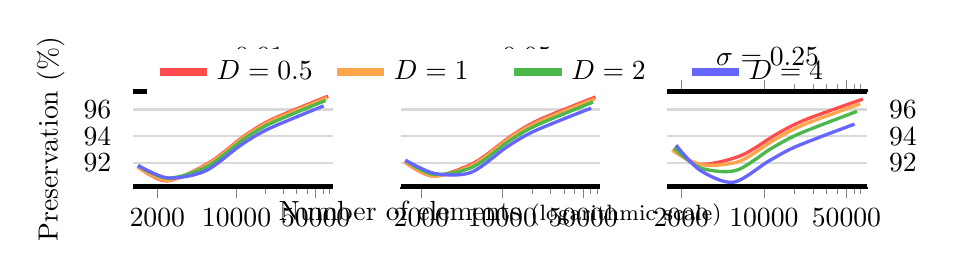
\begin{tikzpicture}
\begin{scope}[shift={(0.0\linewidth,0)}]
\begin{axis}[
 width=0.34\linewidth,height=0.23\linewidth,
 title=\normalsize\mbox{$\sigma=0.01$},
 xmode=log,enlarge x limits=0.025,
 ylabel=Preservation (\%),
 axis y line*=left,
 ymin=90.2097333333,ymax=97.3524633333,
 tick align=outside,
 x axis line style = ultra thick,y axis line style={white},
 xtick={2000,10000,50000},xticklabels={2000,10000,50000},
 minor xtick={18000,26000,34000,42000,58000,66000}, every y tick/.style={white},ymajorgrids,grid style={gray!30,thick}]
\addplot[very thick,mark=none,smooth,color=red!70] table[] {
	1339.73733333 91.7086666667
	2420.84133333 90.6346666667
	5620.72233333 91.9593333333
	11779.2613333 94.029
	20726.7736667 95.2753333333
	64356.625 97.0123333333
};
\addplot[very thick,mark=none,smooth,color=orange!70] table[] {
	1339.73733333 91.7086666667
	2437.06033333 90.6763333333
	5562.499 91.8696666667
	11592.331 93.9196666667
	20332.638 95.1583333333
	63204.0066667 96.8966666667
};
\addplot[very thick,mark=none,smooth,color=green!60!black!70] table[] {
	1353.29366667 91.7726666667
	2475.988 90.8416666667
	5481.227 91.701
	11371.3873333 93.7236666667
	19843.1426667 94.9446666667
	60989.174 96.6806666667
};
\addplot[very thick,mark=none,smooth,color=blue!60!] table[] {
	1350.39633333 91.8063333333
	2464.98566667 90.864
	5298.02166667 91.3796666667
	10942.5643333 93.3313333333
	19078.9953333 94.5446666667
	58686.548 96.2783333333
};
!\end{axis}
\end{scope}
\begin{scope}[shift={(0.28\linewidth,0)}]
\begin{axis}[
 width=0.34\linewidth,height=0.23\linewidth,
 title=\normalsize\mbox{$\sigma=0.05$},
 xmode=log,enlarge x limits=0.025,
 xlabel=Number of elements \footnotesize(logarithmic scale),x label style={at={(axis description cs:0.5,-0.05)},anchor=north},
 yticklabels={},
 legend style={at={(0.55,1.45)},legend style={text width=4em},legend style={draw=none},anchor=north,legend columns=-1},
 axis y line*=left,
 ymin=90.2097333333,ymax=97.3524633333,
 tick align=outside,
 x axis line style = ultra thick,y axis line style={white},
 xtick={2000,10000,50000},xticklabels={2000,10000,50000},
 minor xtick={18000,26000,34000,42000,58000,66000}, every y tick/.style={white},ymajorgrids,grid style={gray!30,thick}]
\addlegendimage{line width=3pt,mark=none,red!70}
\addlegendentry{$D=0.5$}
\addlegendimage{line width=3pt,mark=none,orange!70}
\addlegendentry{$D=1$}
\addlegendimage{line width=3pt,mark=none,green!60!black!70}
\addlegendentry{$D=2$}
\addlegendimage{line width=3pt,mark=none,blue!60!}
\addlegendentry{$D=4$}
\addplot[very thick,mark=none,smooth,color=red!70] table[] {
	1442.82566667 92.0543333333
	2533.24266667 90.9963333333
	5669.485 91.983
	11836.8396667 93.9843333333
	20680.5333333 95.2166666667
	63873.5883333 96.9416666667
};
\addplot[very thick,mark=none,smooth,color=orange!70] table[] {
	1443.78666667 92.0696666667
	2541.81733333 90.9933333333
	5600.65033333 91.8566666667
	11628.1293333 93.8593333333
	20296.073 95.074
	62900.56 96.801
};
\addplot[very thick,mark=none,smooth,color=green!60!black!70] table[] {
	1452.51766667 92.1703333333
	2569.98533333 91.1246666667
	5536.68233333 91.6723333333
	11369.2346667 93.61
	19779.881 94.817
	60739.4833333 96.559
};
\addplot[very thick,mark=none,smooth,color=blue!60!] table[] {
	1456.36 92.2006666667
	2593.726 91.2006666667
	5339.311 91.2663333333
	10949.7836667 93.186
	19062.5516667 94.393
	58616.6363333 96.111
};
!\end{axis}
\end{scope}
\begin{scope}[shift={(0.56\linewidth,0)}]
\begin{axis}[
 width=0.34\linewidth,height=0.23\linewidth,
 title=\normalsize\mbox{$\sigma=0.25$},
 xmode=log,enlarge x limits=0.025,
 axis y line*=right,
 ymin=90.2097333333,ymax=97.3524633333,
 tick align=outside,
 x axis line style = ultra thick,y axis line style={white},
 xtick={2000,10000,50000},xticklabels={2000,10000,50000},
 minor xtick={18000,26000,34000,42000,58000,66000}, every y tick/.style={white},ymajorgrids,grid style={gray!30,thick}]
\addplot[very thick,mark=none,smooth,color=red!70] table[] {
	1691.36433333 92.969
	2904.43666667 91.887
	6401.041 92.5416666667
	13004.1206667 94.1873333333
	22482.168 95.2403333333
	68776.005 96.7843333333
};
\addplot[very thick,mark=none,smooth,color=orange!70] table[] {
	1677.166 92.9476666667
	2901.14533333 91.8643333333
	6100.39133333 92.0893333333
	12251.9936667 93.7186666667
	21241.4256667 94.8286666667
	65459.851 96.4363333333
};
\addplot[very thick,mark=none,smooth,color=green!60!black!70] table[] {
	1735.20633333 93.112
	2860.799 91.636
	5783.71433333 91.421
	11598.037 93.0873333333
	20041.686 94.1946666667
	61282.9063333 95.8633333333
};
\addplot[very thick,mark=none,smooth,color=blue!60!] table[] {
	1804.86366667 93.32
	2875.374 91.4466666667
	5505.542 90.5336666667
	11006.7543333 92.1323333333
	19061.131 93.2513333333
	58545.6053333 94.9093333333
};
!\end{axis}
\end{scope}
\end{tikzpicture}
\end{center}
\caption{Element preservation results using mesh remodelling - NACA 63206 airfoil}\centering\sffamily\footnotesize
Average of thirty optimisation scenarios\end{figure}

\begin{figure}[!h]
\begin{center}
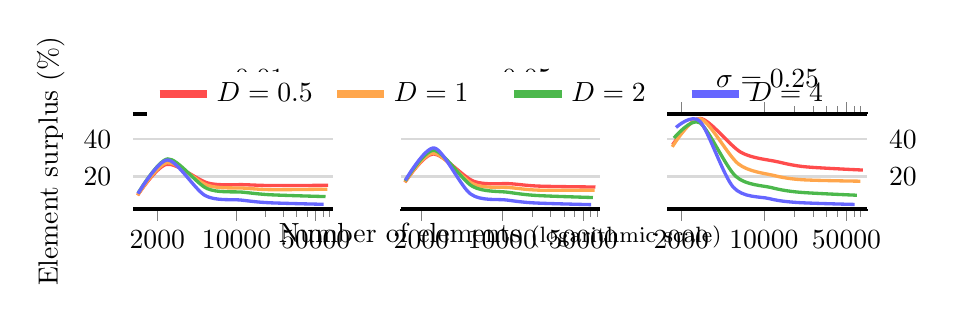
\begin{tikzpicture}
\begin{scope}[shift={(0.0\linewidth,0)}]
\begin{axis}[
 width=0.34\linewidth,height=0.23\linewidth,
 title=\normalsize\mbox{$\sigma=0.01$},
 xmode=log,enlarge x limits=0.025,
 ylabel=Element surplus (\%),
 axis y line*=left,
 ymin=2.69563655211,ymax=53.4657626752,
 tick align=outside,
 x axis line style = ultra thick,y axis line style={white},
 xtick={2000,10000,50000},xticklabels={2000,10000,50000},
 minor xtick={18000,26000,34000,42000,58000,66000}, every y tick/.style={white},ymajorgrids,grid style={gray!30,thick}]
\addplot[very thick,mark=none,smooth,color=red!70] table[] {
	1339.73733333 10.0115945393
	2420.84133333 26.5423126474
	5620.72233333 16.5157546231
	11779.2613333 15.6630938473
	20726.7736667 15.1934227081
	64356.625 15.3350590174
};
\addplot[very thick,mark=none,smooth,color=orange!70] table[] {
	1339.73733333 10.0115945393
	2437.06033333 27.3901128484
	5562.499 15.3088037692
	11592.331 13.8275848051
	20332.638 13.0029304885
	63204.0066667 13.2694239177
};
\addplot[very thick,mark=none,smooth,color=green!60!black!70] table[] {
	1353.29366667 11.124763374
	2475.988 29.4249413595
	5481.227 13.6240615157
	11371.3873333 11.6580915466
	19843.1426667 10.2824567788
	60989.174 9.3001689059
};
\addplot[very thick,mark=none,smooth,color=blue!60!] table[] {
	1350.39633333 10.8868508728
	2464.98566667 28.8498269621
	5298.02166667 9.82627425666
	10942.5643333 7.44738652114
	19078.9953333 6.03554656524
	58686.548 5.17357734513
};
!\end{axis}
\end{scope}
\begin{scope}[shift={(0.28\linewidth,0)}]
\begin{axis}[
 width=0.34\linewidth,height=0.23\linewidth,
 title=\normalsize\mbox{$\sigma=0.05$},
 xmode=log,enlarge x limits=0.025,
 xlabel=Number of elements \footnotesize(logarithmic scale),x label style={at={(axis description cs:0.5,-0.05)},anchor=north},
 yticklabels={},
 legend style={at={(0.55,1.45)},legend style={text width=4em},legend style={draw=none},anchor=north,legend columns=-1},
 axis y line*=left,
 ymin=2.69563655211,ymax=53.4657626752,
 tick align=outside,
 x axis line style = ultra thick,y axis line style={white},
 xtick={2000,10000,50000},xticklabels={2000,10000,50000},
 minor xtick={18000,26000,34000,42000,58000,66000}, every y tick/.style={white},ymajorgrids,grid style={gray!30,thick}]
\addlegendimage{line width=3pt,mark=none,red!70}
\addlegendentry{$D=0.5$}
\addlegendimage{line width=3pt,mark=none,orange!70}
\addlegendentry{$D=1$}
\addlegendimage{line width=3pt,mark=none,green!60!black!70}
\addlegendentry{$D=2$}
\addlegendimage{line width=3pt,mark=none,blue!60!}
\addlegendentry{$D=4$}
\addplot[very thick,mark=none,smooth,color=red!70] table[] {
	1442.82566667 16.9301492289
	2533.24266667 32.0927985122
	5669.485 17.4920768538
	11836.8396667 16.1708317658
	20680.5333333 14.9003842693
	63873.5883333 14.4147493386
};
\addplot[very thick,mark=none,smooth,color=orange!70] table[] {
	1443.78666667 17.0080310382
	2541.81733333 32.5399138759
	5600.65033333 16.0655755144
	11628.1293333 14.1224764865
	20296.073 12.7643349071
	62900.56 12.6717942963
};
\addplot[very thick,mark=none,smooth,color=green!60!black!70] table[] {
	1452.51766667 17.715612804
	2569.98533333 34.0086993174
	5536.68233333 14.7399289747
	11369.2346667 11.5815948311
	19779.881 9.89638860219
	60739.4833333 8.80072565005
};
\addplot[very thick,mark=none,smooth,color=blue!60!] table[] {
	1456.36 18.0270049703
	2593.726 35.2466269505
	5339.311 10.6496865868
	10949.7836667 7.4649578801
	19062.5516667 5.910929682
	58616.6363333 4.99813660305
};
!\end{axis}
\end{scope}
\begin{scope}[shift={(0.56\linewidth,0)}]
\begin{axis}[
 width=0.34\linewidth,height=0.23\linewidth,
 title=\normalsize\mbox{$\sigma=0.25$},
 xmode=log,enlarge x limits=0.025,
 axis y line*=right,
 ymin=2.69563655211,ymax=53.4657626752,
 tick align=outside,
 x axis line style = ultra thick,y axis line style={white},
 xtick={2000,10000,50000},xticklabels={2000,10000,50000},
 minor xtick={18000,26000,34000,42000,58000,66000}, every y tick/.style={white},ymajorgrids,grid style={gray!30,thick}]
\addplot[very thick,mark=none,smooth,color=red!70] table[] {
	1691.36433333 37.0212546477
	2904.43666667 51.0481376217
	6401.041 32.9434040507
	13004.1206667 27.9211229909
	22482.168 25.210606989
	68776.005 23.473751043
};
\addplot[very thick,mark=none,smooth,color=orange!70] table[] {
	1677.166 35.871015513
	2901.14533333 50.8769685355
	6100.39133333 26.6992025039
	12251.9936667 20.5224735214
	21241.4256667 18.3005038053
	65459.851 17.520250641
};
\addplot[very thick,mark=none,smooth,color=green!60!black!70] table[] {
	1735.20633333 40.5729943456
	2860.799 48.7787170639
	5783.71433333 20.1221288116
	11598.037 14.0895225106
	20041.686 11.6187579927
	61282.9063333 10.0213703863
};
\addplot[very thick,mark=none,smooth,color=blue!60!] table[] {
	1804.86366667 46.2160926543
	2875.374 49.5367045357
	5505.542 14.3447596452
	11006.7543333 8.2730936521
	19061.131 6.15772386394
	58545.6053333 5.10708636816
};
!\end{axis}
\end{scope}
\end{tikzpicture}
\end{center}
\caption{Element surplus results on meshes from mesh remodelling - NACA 63206 airfoil}\centering\sffamily\footnotesize
Average of thirty optimisation scenarios\end{figure}

\begin{figure}[!h]
\begin{center}
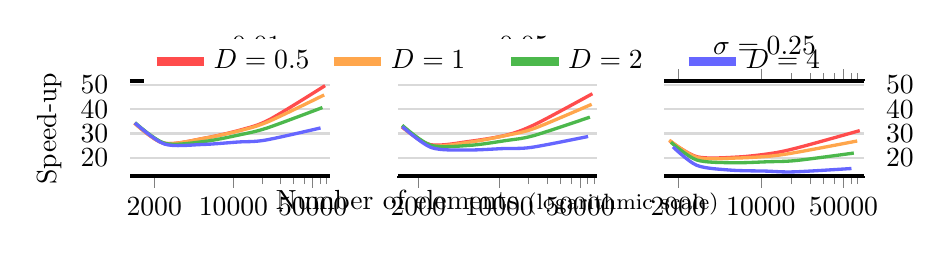
\begin{tikzpicture}
\begin{scope}[shift={(0.0\linewidth,0)}]
\begin{axis}[
 width=0.34\linewidth,height=0.23\linewidth,
 title=\normalsize\mbox{$\sigma=0.01$},
 xmode=log,enlarge x limits=0.025,
 ylabel=Speed-up,
 axis y line*=left,
 ymin=12.4251522816,ymax=51.5637276034,
 tick align=outside,
 x axis line style = ultra thick,y axis line style={white},
 xtick={2000,10000,50000},xticklabels={2000,10000,50000},
 minor xtick={18000,26000,34000,42000,58000,66000}, every y tick/.style={white},ymajorgrids,grid style={gray!30,thick}]
\addplot[very thick,mark=none,smooth,color=red!70] table[] {
	1339.73733333 34.3104912068
	2420.84133333 26.0095823096
	5620.72233333 28.1277017648
	11779.2613333 31.5643828586
	20726.7736667 35.6966932008
	64356.625 49.6999859214
};
\addplot[very thick,mark=none,smooth,color=orange!70] table[] {
	1339.73733333 34.2481840194
	2437.06033333 25.9840451645
	5562.499 28.0581544852
	11592.331 31.2516260163
	20332.638 34.8855543939
	63204.0066667 45.8764132554
};
\addplot[very thick,mark=none,smooth,color=green!60!black!70] table[] {
	1353.29366667 34.4567600487
	2475.988 25.9712953876
	5481.227 26.690751717
	11371.3873333 29.4583772392
	19843.1426667 32.2736530694
	60989.174 40.6851229873
};
\addplot[very thick,mark=none,smooth,color=blue!60!] table[] {
	1350.39633333 34.3521554341
	2464.98566667 25.6441375969
	5298.02166667 25.4641414595
	10942.5643333 26.4860255803
	19078.9953333 27.2636132071
	58686.548 32.2760228571
};
!\end{axis}
\end{scope}
\begin{scope}[shift={(0.28\linewidth,0)}]
\begin{axis}[
 width=0.34\linewidth,height=0.23\linewidth,
 title=\normalsize\mbox{$\sigma=0.05$},
 xmode=log,enlarge x limits=0.025,
 xlabel=Number of elements \footnotesize(logarithmic scale),x label style={at={(axis description cs:0.5,-0.05)},anchor=north},
 yticklabels={},
 legend style={at={(0.55,1.45)},legend style={text width=4em},legend style={draw=none},anchor=north,legend columns=-1},
 axis y line*=left,
 ymin=12.4251522816,ymax=51.5637276034,
 tick align=outside,
 x axis line style = ultra thick,y axis line style={white},
 xtick={2000,10000,50000},xticklabels={2000,10000,50000},
 minor xtick={18000,26000,34000,42000,58000,66000}, every y tick/.style={white},ymajorgrids,grid style={gray!30,thick}]
\addlegendimage{line width=3pt,mark=none,red!70}
\addlegendentry{$D=0.5$}
\addlegendimage{line width=3pt,mark=none,orange!70}
\addlegendentry{$D=1$}
\addlegendimage{line width=3pt,mark=none,green!60!black!70}
\addlegendentry{$D=2$}
\addlegendimage{line width=3pt,mark=none,blue!60!}
\addlegendentry{$D=4$}
\addplot[very thick,mark=none,smooth,color=red!70] table[] {
	1442.82566667 32.7310779817
	2533.24266667 25.4191774271
	5669.485 26.8229473885
	11836.8396667 29.467033232
	20680.5333333 33.8771708431
	63873.5883333 46.3767106526
};
\addplot[very thick,mark=none,smooth,color=orange!70] table[] {
	1443.78666667 32.9388343912
	2541.81733333 25.106991025
	5600.65033333 26.4629247231
	11628.1293333 29.2469720906
	20296.073 32.1646602385
	62900.56 42.0141885094
};
\addplot[very thick,mark=none,smooth,color=green!60!black!70] table[] {
	1452.51766667 33.381871345
	2569.98533333 25.1545196403
	5536.68233333 25.098905012
	11369.2346667 27.0746731664
	19779.881 29.0930202555
	60739.4833333 36.7308996847
};
\addplot[very thick,mark=none,smooth,color=blue!60!] table[] {
	1456.36 32.825186889
	2593.726 24.2092917331
	5339.311 23.2026993663
	10949.7836667 23.8044028833
	19062.5516667 24.2953801069
	58616.6363333 28.7689244656
};
!\end{axis}
\end{scope}
\begin{scope}[shift={(0.56\linewidth,0)}]
\begin{axis}[
 width=0.34\linewidth,height=0.23\linewidth,
 title=\normalsize\mbox{$\sigma=0.25$},
 xmode=log,enlarge x limits=0.025,
 axis y line*=right,
 ymin=12.4251522816,ymax=51.5637276034,
 tick align=outside,
 x axis line style = ultra thick,y axis line style={white},
 xtick={2000,10000,50000},xticklabels={2000,10000,50000},
 minor xtick={18000,26000,34000,42000,58000,66000}, every y tick/.style={white},ymajorgrids,grid style={gray!30,thick}]
\addplot[very thick,mark=none,smooth,color=red!70] table[] {
	1691.36433333 27.0462345091
	2904.43666667 20.3891912908
	6401.041 20.315700412
	13004.1206667 22.0015482729
	22482.168 24.6333959395
	68776.005 31.1853215513
};
\addplot[very thick,mark=none,smooth,color=orange!70] table[] {
	1677.166 27.2802884615
	2901.14533333 20.1193170919
	6100.39133333 19.8755488375
	12251.9936667 20.7241918122
	21241.4256667 22.4516812717
	65459.851 26.9171610169
};
\addplot[very thick,mark=none,smooth,color=green!60!black!70] table[] {
	1735.20633333 26.3920930233
	2860.799 19.1146345909
	5783.71433333 17.9597398374
	11598.037 18.3726643066
	20041.686 18.8864622084
	61282.9063333 21.9434308726
};
\addplot[very thick,mark=none,smooth,color=blue!60!] table[] {
	1804.86366667 24.4898575744
	2875.374 16.8864917083
	5505.542 14.9324572788
	11006.7543333 14.5173185445
	19061.131 14.2001443597
	58545.6053333 15.5812877199
};
!\end{axis}
\end{scope}
\end{tikzpicture}
\end{center}
\caption{Speed-up results by mesh remodelling - NACA 63206 airfoil}\centering\sffamily\footnotesize
Average of thirty optimisation scenarios\end{figure}

\pagebreak
\subsubsection{Eppler 376}
\vspace*{\fill} \begin{table}[!hp]
\begin{center}
\begin{tabular}{c|cc?c|c?c?c|c|c||c|c}
\multirow{2}{*}{\textbf{\large $\boldsymbol{\sigma}$}} & \multirow{2}{*}{\textbf{\large $\boldsymbol{I}$}} & \multirow{2}{*}{\textbf{\large $\boldsymbol{G}$}} & \multicolumn{2}{c?}{\textbf{\large Generation}} & \multirow{2}{*}{\textbf{\large $\boldsymbol{D}$}} & \multicolumn{5}{c}{\textbf{{\large Remodelling} }} \\\cline{4-5}\cline{7-11}
 & & & \textbf{\# Tri.} & \textbf{Time} & &\textbf{\# Tri.} & \textbf{Time} & \textbf{Preserv.} & \textbf{+ Tri.} & \textbf{Sp.-up} \\\toprule
\multirow{24}[13]{*}{.01} & \multirow{4}{*}{50} & \multirow{4}{*}{1} & \multirow{4}{*}{1210} & \multirow{4}{*}{1.78 ms} & .5 & 1598 & 0.07 ms & 92.70 \% & 32.00 \% & 25.53 \\\cline{6-11}
 & & & &  & 1 & 1585 & 0.07 ms & 92.66 \% & 30.99 \% & 25.95 \\\cline{6-11}
 & & & &  & 2 & 1616 & 0.07 ms & 92.77 \% & 33.51 \% & 25.71 \\\cline{6-11}
 & & & &  & 4 & 1614 & 0.07 ms & 92.70 \% & 33.39 \% & 24.76 \\\cmidrule[1.5pt]{2-11}
 & \multirow{4}{*}{100} & \multirow{4}{*}{2} & \multirow{4}{*}{1934} & \multirow{4}{*}{3.27 ms} & .5 & 2740 & 0.17 ms & 91.52 \% & 41.65 \% & 18.78 \\\cline{6-11}
 & & & &  & 1 & 2714 & 0.17 ms & 91.44 \% & 40.30 \% & 18.72 \\\cline{6-11}
 & & & &  & 2 & 2715 & 0.18 ms & 91.42 \% & 40.35 \% & 18.41 \\\cline{6-11}
 & & & &  & 4 & 2738 & 0.19 ms & 91.33 \% & 41.56 \% & 17.38 \\\cmidrule[1.5pt]{2-11}
 & \multirow{4}{*}{200} & \multirow{4}{*}{4} & \multirow{4}{*}{4768} & \multirow{4}{*}{8.41 ms} & .5 & 6220 & 0.48 ms & 92.43 \% & 30.44 \% & 17.58 \\\cline{6-11}
 & & & &  & 1 & 5987 & 0.48 ms & 92.11 \% & 25.55 \% & 17.63 \\\cline{6-11}
 & & & &  & 2 & 5687 & 0.51 ms & 91.54 \% & 19.26 \% & 16.48 \\\cline{6-11}
 & & & &  & 4 & 5399 & 0.58 ms & 90.73 \% & 13.22 \% & 14.58 \\\cmidrule[1.5pt]{2-11}
 & \multirow{4}{*}{300} & \multirow{4}{*}{6} & \multirow{4}{*}{10103} & \multirow{4}{*}{18.17 ms} & .5 & 12841 & 0.97 ms & 94.19 \% & 27.10 \% & 18.68 \\\cline{6-11}
 & & & &  & 1 & 12307 & 1.00 ms & 93.88 \% & 21.82 \% & 18.09 \\\cline{6-11}
 & & & &  & 2 & 11575 & 1.10 ms & 93.29 \% & 14.57 \% & 16.47 \\\cline{6-11}
 & & & &  & 4 & 11013 & 1.31 ms & 92.48 \% & 9.01 \% & 13.91 \\\cmidrule[1.5pt]{2-11}
 & \multirow{4}{*}{400} & \multirow{4}{*}{8} & \multirow{4}{*}{17867} & \multirow{4}{*}{33.71 ms} & .5 & 22453 & 1.62 ms & 95.31 \% & 25.67 \% & 20.76 \\\cline{6-11}
 & & & &  & 1 & 21450 & 1.72 ms & 94.98 \% & 20.05 \% & 19.56 \\\cline{6-11}
 & & & &  & 2 & 20057 & 1.93 ms & 94.42 \% & 12.26 \% & 17.50 \\\cline{6-11}
 & & & &  & 4 & 19064 & 2.45 ms & 93.58 \% & 6.70 \% & 13.78 \\\cmidrule[1.5pt]{2-11}
 & \multirow{4}{*}{700} & \multirow{4}{*}{14} & \multirow{4}{*}{55533} & \multirow{4}{*}{151.14 ms} & .5 & 69114 & 5.52 ms & 96.85 \% & 24.46 \% & 27.37 \\\cline{6-11}
 & & & &  & 1 & 66056 & 6.13 ms & 96.55 \% & 18.95 \% & 24.66 \\\cline{6-11}
 & & & &  & 2 & 61394 & 7.01 ms & 96.06 \% & 10.55 \% & 21.56 \\\cline{6-11}
 & & & &  & 4 & 58530 & 9.56 ms & 95.19 \% & 5.40 \% & 15.82\\\bottomrule
\end{tabular}\end{center}
\caption{Full results of mesh remodelling for $\sigma=0.01$ - Eppler 376 airfoil}\centering\sffamily\footnotesize
Average of thirty optimisation scenarios\end{table}
 \vspace*{\fill}
\begin{table}[!hp]
\begin{center}
\begin{tabular}{c|cc?c|c?c?c|c|c||c|c}
\multirow{2}{*}{\textbf{\large $\boldsymbol{\sigma}$}} & \multirow{2}{*}{\textbf{\large $\boldsymbol{I}$}} & \multirow{2}{*}{\textbf{\large $\boldsymbol{G}$}} & \multicolumn{2}{c?}{\textbf{\large Generation}} & \multirow{2}{*}{\textbf{\large $\boldsymbol{D}$}} & \multicolumn{5}{c}{\textbf{{\large Remodelling} }} \\\cline{4-5}\cline{7-11}
 & & & \textbf{\# Tri.} & \textbf{Time} & &\textbf{\# Tri.} & \textbf{Time} & \textbf{Preserv.} & \textbf{+ Tri.} & \textbf{Sp.-up} \\\toprule
\multirow{24}[11]{*}{.05} & \multirow{4}{*}{50} & \multirow{4}{*}{1} & \multirow{4}{*}{1210} & \multirow{4}{*}{1.77 ms} & .5 & 1608 & 0.07 ms & 92.70 \% & 32.95 \% & 24.47 \\\cline{6-11}
 & & & &  & 1 & 1594 & 0.07 ms & 92.61 \% & 31.80 \% & 24.49 \\\cline{6-11}
 & & & &  & 2 & 1605 & 0.07 ms & 92.63 \% & 32.66 \% & 24.61 \\\cline{6-11}
 & & & &  & 4 & 1647 & 0.07 ms & 92.82 \% & 36.17 \% & 23.77 \\\cmidrule[1.5pt]{2-11}
 & \multirow{4}{*}{100} & \multirow{4}{*}{2} & \multirow{4}{*}{1936} & \multirow{4}{*}{3.27 ms} & .5 & 2816 & 0.18 ms & 91.71 \% & 45.45 \% & 18.20 \\\cline{6-11}
 & & & &  & 1 & 2784 & 0.18 ms & 91.63 \% & 43.83 \% & 18.02 \\\cline{6-11}
 & & & &  & 2 & 2771 & 0.18 ms & 91.55 \% & 43.15 \% & 17.83 \\\cline{6-11}
 & & & &  & 4 & 2748 & 0.20 ms & 91.28 \% & 41.97 \% & 16.31 \\\cmidrule[1.5pt]{2-11}
 & \multirow{4}{*}{200} & \multirow{4}{*}{4} & \multirow{4}{*}{4767} & \multirow{4}{*}{8.37 ms} & .5 & 6255 & 0.49 ms & 92.41 \% & 31.20 \% & 16.99 \\\cline{6-11}
 & & & &  & 1 & 6009 & 0.49 ms & 92.06 \% & 26.04 \% & 16.95 \\\cline{6-11}
 & & & &  & 2 & 5749 & 0.54 ms & 91.52 \% & 20.60 \% & 15.56 \\\cline{6-11}
 & & & &  & 4 & 5426 & 0.61 ms & 90.63 \% & 13.83 \% & 13.79 \\\cmidrule[1.5pt]{2-11}
 & \multirow{4}{*}{300} & \multirow{4}{*}{6} & \multirow{4}{*}{10101} & \multirow{4}{*}{18.10 ms} & .5 & 12940 & 1.01 ms & 94.17 \% & 28.10 \% & 17.90 \\\cline{6-11}
 & & & &  & 1 & 12319 & 1.05 ms & 93.80 \% & 21.95 \% & 17.31 \\\cline{6-11}
 & & & &  & 2 & 11598 & 1.15 ms & 93.19 \% & 14.82 \% & 15.76 \\\cline{6-11}
 & & & &  & 4 & 11030 & 1.38 ms & 92.33 \% & 9.20 \% & 13.11 \\\cmidrule[1.5pt]{2-11}
 & \multirow{4}{*}{400} & \multirow{4}{*}{8} & \multirow{4}{*}{17863} & \multirow{4}{*}{33.60 ms} & .5 & 22515 & 1.67 ms & 95.25 \% & 26.04 \% & 20.14 \\\cline{6-11}
 & & & &  & 1 & 21445 & 1.78 ms & 94.90 \% & 20.05 \% & 18.86 \\\cline{6-11}
 & & & &  & 2 & 20081 & 2.02 ms & 94.31 \% & 12.42 \% & 16.66 \\\cline{6-11}
 & & & &  & 4 & 19092 & 2.60 ms & 93.42 \% & 6.88 \% & 12.93 \\\cmidrule[1.5pt]{2-11}
 & \multirow{4}{*}{700} & \multirow{4}{*}{14} & \multirow{4}{*}{55526} & \multirow{4}{*}{151.14 ms} & .5 & 69029 & 5.74 ms & 96.79 \% & 24.32 \% & 26.34 \\\cline{6-11}
 & & & &  & 1 & 65971 & 6.41 ms & 96.47 \% & 18.81 \% & 23.57 \\\cline{6-11}
 & & & &  & 2 & 61432 & 7.47 ms & 95.94 \% & 10.64 \% & 20.24 \\\cline{6-11}
 & & & &  & 4 & 58570 & 10.22 ms & 95.01 \% & 5.48 \% & 14.79\\\bottomrule
\end{tabular}\end{center}
\caption{Full results of mesh remodelling for $\sigma=0.05$ - Eppler 376 airfoil}\centering\sffamily\footnotesize
Average of thirty optimisation scenarios\end{table}

\begin{table}[!hp]
\begin{center}
\begin{tabular}{c|cc?c|c?c?c|c|c||c|c}
\multirow{2}{*}{\textbf{\large $\boldsymbol{\sigma}$}} & \multirow{2}{*}{\textbf{\large $\boldsymbol{I}$}} & \multirow{2}{*}{\textbf{\large $\boldsymbol{G}$}} & \multicolumn{2}{c?}{\textbf{\large Generation}} & \multirow{2}{*}{\textbf{\large $\boldsymbol{D}$}} & \multicolumn{5}{c}{\textbf{{\large Remodelling} }} \\\cline{4-5}\cline{7-11}
 & & & \textbf{\# Tri.} & \textbf{Time} & &\textbf{\# Tri.} & \textbf{Time} & \textbf{Preserv.} & \textbf{+ Tri.} & \textbf{Sp.-up} \\\toprule
\multirow{24}[13]{*}{.25} & \multirow{4}{*}{50} & \multirow{4}{*}{1} & \multirow{4}{*}{1207} & \multirow{4}{*}{1.77 ms} & .5 & 1730 & 0.08 ms & 93.15 \% & 43.27 \% & 23.10 \\\cline{6-11}
 & & & &  & 1 & 1730 & 0.08 ms & 93.15 \% & 43.31 \% & 22.96 \\\cline{6-11}
 & & & &  & 2 & 1773 & 0.08 ms & 93.24 \% & 46.83 \% & 22.07 \\\cline{6-11}
 & & & &  & 4 & 1825 & 0.09 ms & 93.32 \% & 51.15 \% & 20.51 \\\cmidrule[1.5pt]{2-11}
 & \multirow{4}{*}{100} & \multirow{4}{*}{2} & \multirow{4}{*}{1938} & \multirow{4}{*}{3.25 ms} & .5 & 2962 & 0.19 ms & 92.05 \% & 52.85 \% & 17.55 \\\cline{6-11}
 & & & &  & 1 & 2923 & 0.19 ms & 91.90 \% & 50.82 \% & 17.34 \\\cline{6-11}
 & & & &  & 2 & 2923 & 0.20 ms & 91.78 \% & 50.84 \% & 16.22 \\\cline{6-11}
 & & & &  & 4 & 2863 & 0.23 ms & 91.27 \% & 47.74 \% & 13.87 \\\cmidrule[1.5pt]{2-11}
 & \multirow{4}{*}{200} & \multirow{4}{*}{4} & \multirow{4}{*}{4764} & \multirow{4}{*}{8.34 ms} & .5 & 6693 & 0.52 ms & 92.77 \% & 40.50 \% & 16.11 \\\cline{6-11}
 & & & &  & 1 & 6279 & 0.53 ms & 92.19 \% & 31.81 \% & 15.75 \\\cline{6-11}
 & & & &  & 2 & 5860 & 0.59 ms & 91.38 \% & 23.01 \% & 14.14 \\\cline{6-11}
 & & & &  & 4 & 5562 & 0.71 ms & 90.32 \% & 16.76 \% & 11.76 \\\cmidrule[1.5pt]{2-11}
 & \multirow{4}{*}{300} & \multirow{4}{*}{6} & \multirow{4}{*}{10089} & \multirow{4}{*}{18.02 ms} & .5 & 13606 & 1.07 ms & 94.31 \% & 34.86 \% & 16.90 \\\cline{6-11}
 & & & &  & 1 & 12649 & 1.12 ms & 93.77 \% & 25.38 \% & 16.05 \\\cline{6-11}
 & & & &  & 2 & 11707 & 1.28 ms & 92.95 \% & 16.04 \% & 14.10 \\\cline{6-11}
 & & & &  & 4 & 11066 & 1.61 ms & 91.80 \% & 9.69 \% & 11.21 \\\cmidrule[1.5pt]{2-11}
 & \multirow{4}{*}{400} & \multirow{4}{*}{8} & \multirow{4}{*}{17845} & \multirow{4}{*}{33.46 ms} & .5 & 23499 & 1.77 ms & 95.31 \% & 31.68 \% & 18.87 \\\cline{6-11}
 & & & &  & 1 & 21894 & 1.94 ms & 94.81 \% & 22.69 \% & 17.26 \\\cline{6-11}
 & & & &  & 2 & 20180 & 2.31 ms & 94.03 \% & 13.09 \% & 14.50 \\\cline{6-11}
 & & & &  & 4 & 19062 & 3.09 ms & 92.85 \% & 6.82 \% & 10.83 \\\cmidrule[1.5pt]{2-11}
 & \multirow{4}{*}{700} & \multirow{4}{*}{14} & \multirow{4}{*}{55458} & \multirow{4}{*}{150.16 ms} & .5 & 71718 & 6.26 ms & 96.77 \% & 29.32 \% & 23.98 \\\cline{6-11}
 & & & &  & 1 & 67278 & 7.18 ms & 96.35 \% & 21.31 \% & 20.93 \\\cline{6-11}
 & & & &  & 2 & 61629 & 8.65 ms & 95.64 \% & 11.13 \% & 17.36 \\\cline{6-11}
 & & & &  & 4 & 58557 & 12.39 ms & 94.44 \% & 5.59 \% & 12.12\\\bottomrule
\end{tabular}\end{center}
\caption{Full results of mesh remodelling for $\sigma=0.25$ - Eppler 376 airfoil}\centering\sffamily\footnotesize
Average of thirty optimisation scenarios\end{table}
 \newpage
\begin{figure}[!h]
\begin{center}
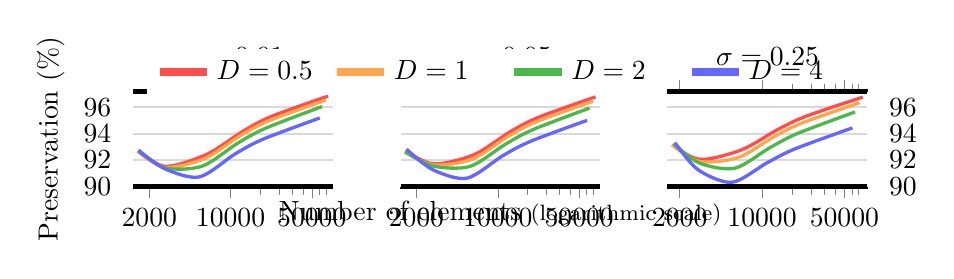
\begin{tikzpicture}
\begin{scope}[shift={(0.0\linewidth,0)}]
\begin{axis}[
 width=0.34\linewidth,height=0.23\linewidth,
 title=\normalsize\mbox{$\sigma=0.01$},
 xmode=log,enlarge x limits=0.025,
 ylabel=Preservation (\%),
 axis y line*=left,
 ymin=89.9891,ymax=97.189895,
 tick align=outside,
 x axis line style = ultra thick,y axis line style={white},
 xtick={2000,10000,50000},xticklabels={2000,10000,50000},
 minor xtick={18000,26000,34000,42000,58000,66000}, every y tick/.style={white},ymajorgrids,grid style={gray!30,thick}]
\addplot[very thick,mark=none,smooth,color=red!70] table[] {
	1597.56966667 92.6966666667
	2740.0 91.5226666667
	6219.95666667 92.427
	12841.0846667 94.191
	22453.2753333 95.3053333333
	69114.4313333 96.847
};
\addplot[very thick,mark=none,smooth,color=orange!70] table[] {
	1585.37333333 92.6606666667
	2713.76166667 91.445
	5986.56433333 92.1116666667
	12307.4733333 93.88
	21449.891 94.9793333333
	66056.1383333 96.5516666667
};
\addplot[very thick,mark=none,smooth,color=green!60!black!70] table[] {
	1615.85633333 92.7716666667
	2714.83633333 91.417
	5686.62733333 91.5383333333
	11574.5646667 93.2903333333
	20057.094 94.4156666667
	61394.3783333 96.057
};
\addplot[very thick,mark=none,smooth,color=blue!60!] table[] {
	1614.35233333 92.7013333333
	2738.08866667 91.332
	5399.01866667 90.7253333333
	11013.093 92.482
	19064.4793333 93.584
	58529.946 95.1883333333
};
!\end{axis}
\end{scope}
\begin{scope}[shift={(0.28\linewidth,0)}]
\begin{axis}[
 width=0.34\linewidth,height=0.23\linewidth,
 title=\normalsize\mbox{$\sigma=0.05$},
 xmode=log,enlarge x limits=0.025,
 xlabel=Number of elements \footnotesize(logarithmic scale),x label style={at={(axis description cs:0.5,-0.05)},anchor=north},
 yticklabels={},
 legend style={at={(0.55,1.45)},legend style={text width=4em},legend style={draw=none},anchor=north,legend columns=-1},
 axis y line*=left,
 ymin=89.9891,ymax=97.189895,
 tick align=outside,
 x axis line style = ultra thick,y axis line style={white},
 xtick={2000,10000,50000},xticklabels={2000,10000,50000},
 minor xtick={18000,26000,34000,42000,58000,66000}, every y tick/.style={white},ymajorgrids,grid style={gray!30,thick}]
\addlegendimage{line width=3pt,mark=none,red!70}
\addlegendentry{$D=0.5$}
\addlegendimage{line width=3pt,mark=none,orange!70}
\addlegendentry{$D=1$}
\addlegendimage{line width=3pt,mark=none,green!60!black!70}
\addlegendentry{$D=2$}
\addlegendimage{line width=3pt,mark=none,blue!60!}
\addlegendentry{$D=4$}
\addplot[very thick,mark=none,smooth,color=red!70] table[] {
	1608.38566667 92.7036666667
	2815.783 91.7103333333
	6254.791 92.4063333333
	12939.9666667 94.1726666667
	22515.0153333 95.248
	69028.7106667 96.7856666667
};
\addplot[very thick,mark=none,smooth,color=orange!70] table[] {
	1594.41933333 92.6116666667
	2784.365 91.634
	6008.57 92.062
	12318.54 93.797
	21444.6516667 94.9023333333
	65971.1733333 96.4693333333
};
\addplot[very thick,mark=none,smooth,color=green!60!black!70] table[] {
	1604.80333333 92.6296666667
	2771.266 91.5523333333
	5749.36966667 91.5163333333
	11597.869 93.193
	20081.009 94.3106666667
	61432.4436667 95.94
};
\addplot[very thick,mark=none,smooth,color=blue!60!] table[] {
	1647.27933333 92.823
	2748.387 91.2833333333
	5426.47433333 90.6263333333
	11030.181 92.3283333333
	19092.137 93.4203333333
	58569.6863333 95.0116666667
};
!\end{axis}
\end{scope}
\begin{scope}[shift={(0.56\linewidth,0)}]
\begin{axis}[
 width=0.34\linewidth,height=0.23\linewidth,
 title=\normalsize\mbox{$\sigma=0.25$},
 xmode=log,enlarge x limits=0.025,
 axis y line*=right,
 ymin=89.9891,ymax=97.189895,
 tick align=outside,
 x axis line style = ultra thick,y axis line style={white},
 xtick={2000,10000,50000},xticklabels={2000,10000,50000},
 minor xtick={18000,26000,34000,42000,58000,66000}, every y tick/.style={white},ymajorgrids,grid style={gray!30,thick}]
\addplot[very thick,mark=none,smooth,color=red!70] table[] {
	1729.68166667 93.151
	2962.25533333 92.0506666667
	6692.924 92.771
	13605.839 94.3123333333
	23499.072 95.31
	71717.803 96.7676666667
};
\addplot[very thick,mark=none,smooth,color=orange!70] table[] {
	1730.17 93.152
	2922.996 91.9006666667
	6278.947 92.192
	12649.4086667 93.773
	21893.7756667 94.8106666667
	67277.523 96.3466666667
};
\addplot[very thick,mark=none,smooth,color=green!60!black!70] table[] {
	1772.74233333 93.2436666667
	2923.30333333 91.7846666667
	5859.619 91.3836666667
	11707.061 92.9486666667
	20179.976 94.029
	61628.7326667 95.643
};
\addplot[very thick,mark=none,smooth,color=blue!60!] table[] {
	1824.84966667 93.317
	2863.199 91.269
	5561.88933333 90.3156666667
	11065.8646667 91.8006666667
	19061.8436667 92.8496666667
	58557.4696667 94.4393333333
};
!\end{axis}
\end{scope}
\end{tikzpicture}
\end{center}
\caption{Element preservation results using mesh remodelling - Eppler 376 airfoil}\centering\sffamily\footnotesize
Average of thirty optimisation scenarios\end{figure}

\begin{figure}[!h]
\begin{center}
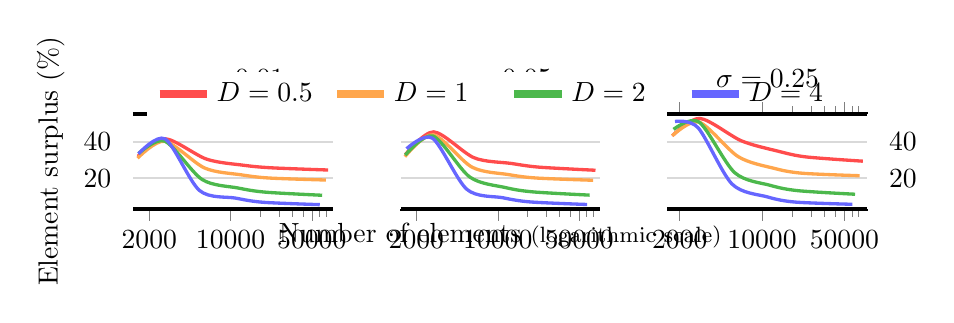
\begin{tikzpicture}
\begin{scope}[shift={(0.0\linewidth,0)}]
\begin{axis}[
 width=0.34\linewidth,height=0.23\linewidth,
 title=\normalsize\mbox{$\sigma=0.01$},
 xmode=log,enlarge x limits=0.025,
 ylabel=Element surplus (\%),
 axis y line*=left,
 ymin=3.02435880427,ymax=55.3384618855,
 tick align=outside,
 x axis line style = ultra thick,y axis line style={white},
 xtick={2000,10000,50000},xticklabels={2000,10000,50000},
 minor xtick={18000,26000,34000,42000,58000,66000}, every y tick/.style={white},ymajorgrids,grid style={gray!30,thick}]
\addplot[very thick,mark=none,smooth,color=red!70] table[] {
	1597.56966667 31.9986240243
	2740.0 41.6548979938
	6219.95666667 30.4411864834
	12841.0846667 27.1014265864
	22453.2753333 25.6667617441
	69114.4313333 24.4567261192
};
\addplot[very thick,mark=none,smooth,color=orange!70] table[] {
	1585.37333333 30.9909063317
	2713.76166667 40.2984058654
	5986.56433333 25.5466229828
	12307.4733333 21.8197262106
	21449.891 20.0510082256
	66056.1383333 18.9495530593
};
\addplot[very thick,mark=none,smooth,color=green!60!black!70] table[] {
	1615.85633333 33.5095533367
	2714.83633333 40.3539649154
	5686.62733333 19.2565247961
	11574.5646667 14.5653750784
	20057.094 12.2557852054
	61394.3783333 10.5549619969
};
\addplot[very thick,mark=none,smooth,color=blue!60!] table[] {
	1614.35233333 33.385285873
	2738.08866667 41.5560842243
	5399.01866667 13.2249689938
	11013.093 9.0079123193
	19064.4793333 6.70030748699
	58529.946 5.39688048596
};
!\end{axis}
\end{scope}
\begin{scope}[shift={(0.28\linewidth,0)}]
\begin{axis}[
 width=0.34\linewidth,height=0.23\linewidth,
 title=\normalsize\mbox{$\sigma=0.05$},
 xmode=log,enlarge x limits=0.025,
 xlabel=Number of elements \footnotesize(logarithmic scale),x label style={at={(axis description cs:0.5,-0.05)},anchor=north},
 yticklabels={},
 legend style={at={(0.55,1.45)},legend style={text width=4em},legend style={draw=none},anchor=north,legend columns=-1},
 axis y line*=left,
 ymin=3.02435880427,ymax=55.3384618855,
 tick align=outside,
 x axis line style = ultra thick,y axis line style={white},
 xtick={2000,10000,50000},xticklabels={2000,10000,50000},
 minor xtick={18000,26000,34000,42000,58000,66000}, every y tick/.style={white},ymajorgrids,grid style={gray!30,thick}]
\addlegendimage{line width=3pt,mark=none,red!70}
\addlegendentry{$D=0.5$}
\addlegendimage{line width=3pt,mark=none,orange!70}
\addlegendentry{$D=1$}
\addlegendimage{line width=3pt,mark=none,green!60!black!70}
\addlegendentry{$D=2$}
\addlegendimage{line width=3pt,mark=none,blue!60!}
\addlegendentry{$D=4$}
\addplot[very thick,mark=none,smooth,color=red!70] table[] {
	1608.38566667 32.9528205058
	2815.783 45.4530787272
	6254.791 31.2000785898
	12939.9666667 28.103553345
	22515.0153333 26.0419465148
	69028.7106667 24.3168789276
};
\addplot[very thick,mark=none,smooth,color=orange!70] table[] {
	1594.41933333 31.7983315997
	2784.365 43.8301394498
	6008.57 26.0353633259
	12318.54 21.9515309949
	21444.6516667 20.0499132859
	65971.1733333 18.8104237901
};
\addplot[very thick,mark=none,smooth,color=green!60!black!70] table[] {
	1604.80333333 32.6566966777
	2771.266 43.1534928906
	5749.36966667 20.5983944321
	11597.869 14.8170059786
	20081.009 12.4160665613
	61432.4436667 10.6364234212
};
\addplot[very thick,mark=none,smooth,color=blue!60!] table[] {
	1647.27933333 36.1678595292
	2748.387 41.9716472057
	5426.47433333 13.8253634692
	11030.181 9.19698763817
	19092.137 6.88023414508
	58569.6863333 5.48075625935
};
!\end{axis}
\end{scope}
\begin{scope}[shift={(0.56\linewidth,0)}]
\begin{axis}[
 width=0.34\linewidth,height=0.23\linewidth,
 title=\normalsize\mbox{$\sigma=0.25$},
 xmode=log,enlarge x limits=0.025,
 axis y line*=right,
 ymin=3.02435880427,ymax=55.3384618855,
 tick align=outside,
 x axis line style = ultra thick,y axis line style={white},
 xtick={2000,10000,50000},xticklabels={2000,10000,50000},
 minor xtick={18000,26000,34000,42000,58000,66000}, every y tick/.style={white},ymajorgrids,grid style={gray!30,thick}]
\addplot[very thick,mark=none,smooth,color=red!70] table[] {
	1729.68166667 43.2665314173
	2962.25533333 52.8473141197
	6692.924 40.5041679038
	13605.839 34.8624344269
	23499.072 31.6848749521
	71717.803 29.319428268
};
\addplot[very thick,mark=none,smooth,color=orange!70] table[] {
	1730.17 43.30697922
	2922.996 50.8215995952
	6278.947 31.813572595
	12649.4086667 25.3822014833
	21893.7756667 22.6890623977
	67277.523 21.3128462628
};
\addplot[very thick,mark=none,smooth,color=green!60!black!70] table[] {
	1772.74233333 46.8331717262
	2923.30333333 50.8374574701
	5859.619 23.0106440516
	11707.061 16.0415573376
	20179.976 13.0852152841
	61628.7326667 11.1271140491
};
\addplot[very thick,mark=none,smooth,color=blue!60!] table[] {
	1824.84966667 51.1491317389
	2863.199 47.7361765597
	5561.88933333 16.7604223136
	11065.8646667 9.68595527152
	19061.8436667 6.81938842531
	58557.4696667 5.58910314241
};
!\end{axis}
\end{scope}
\end{tikzpicture}
\end{center}
\caption{Element surplus results on meshes from mesh remodelling - Eppler 376 airfoil}\centering\sffamily\footnotesize
Average of thirty optimisation scenarios\end{figure}

\begin{figure}[!h]
\begin{center}
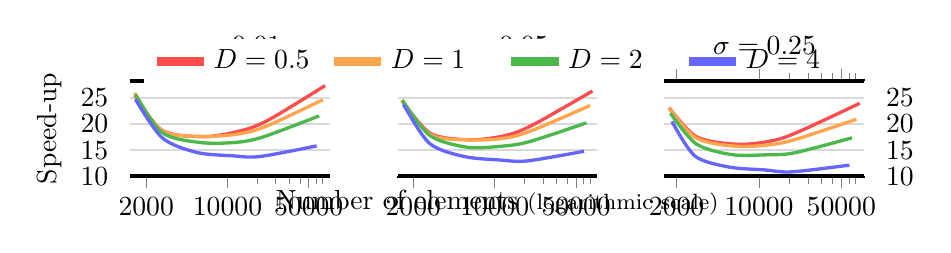
\begin{tikzpicture}
\begin{scope}[shift={(0.0\linewidth,0)}]
\begin{axis}[
 width=0.34\linewidth,height=0.23\linewidth,
 title=\normalsize\mbox{$\sigma=0.01$},
 xmode=log,enlarge x limits=0.025,
 ylabel=Speed-up,
 axis y line*=left,
 ymin=10.0051597471,ymax=28.2408860444,
 tick align=outside,
 x axis line style = ultra thick,y axis line style={white},
 xtick={2000,10000,50000},xticklabels={2000,10000,50000},
 minor xtick={18000,26000,34000,42000,58000,66000}, every y tick/.style={white},ymajorgrids,grid style={gray!30,thick}]
\addplot[very thick,mark=none,smooth,color=red!70] table[] {
	1597.56966667 25.5275251316
	2740.0 18.7841823056
	6219.95666667 17.5804429586
	12841.0846667 18.6768877621
	22453.2753333 20.7637856703
	69114.4313333 27.3725181255
};
\addplot[very thick,mark=none,smooth,color=orange!70] table[] {
	1585.37333333 25.9498783455
	2713.76166667 18.7160847167
	5986.56433333 17.6344837222
	12307.4733333 18.0905621557
	21449.891 19.5640752848
	66056.1383333 24.6605445211
};
\addplot[very thick,mark=none,smooth,color=green!60!black!70] table[] {
	1615.85633333 25.7121504339
	2714.83633333 18.4070182023
	5686.62733333 16.4818805093
	11574.5646667 16.4744938048
	20057.094 17.5046989391
	61394.3783333 21.5595966032
};
\addplot[very thick,mark=none,smooth,color=blue!60!] table[] {
	1614.35233333 24.7571959146
	2738.08866667 17.3827751196
	5399.01866667 14.5755860954
	11013.093 13.9126917286
	19064.4793333 13.7776566906
	58529.946 15.816096244
};
!\end{axis}
\end{scope}
\begin{scope}[shift={(0.28\linewidth,0)}]
\begin{axis}[
 width=0.34\linewidth,height=0.23\linewidth,
 title=\normalsize\mbox{$\sigma=0.05$},
 xmode=log,enlarge x limits=0.025,
 xlabel=Number of elements \footnotesize(logarithmic scale),x label style={at={(axis description cs:0.5,-0.05)},anchor=north},
 yticklabels={},
 legend style={at={(0.55,1.45)},legend style={text width=4em},legend style={draw=none},anchor=north,legend columns=-1},
 axis y line*=left,
 ymin=10.0051597471,ymax=28.2408860444,
 tick align=outside,
 x axis line style = ultra thick,y axis line style={white},
 xtick={2000,10000,50000},xticklabels={2000,10000,50000},
 minor xtick={18000,26000,34000,42000,58000,66000}, every y tick/.style={white},ymajorgrids,grid style={gray!30,thick}]
\addlegendimage{line width=3pt,mark=none,red!70}
\addlegendentry{$D=0.5$}
\addlegendimage{line width=3pt,mark=none,orange!70}
\addlegendentry{$D=1$}
\addlegendimage{line width=3pt,mark=none,green!60!black!70}
\addlegendentry{$D=2$}
\addlegendimage{line width=3pt,mark=none,blue!60!}
\addlegendentry{$D=4$}
\addplot[very thick,mark=none,smooth,color=red!70] table[] {
	1608.38566667 24.4659926471
	2815.783 18.1956562094
	6254.791 16.9864033011
	12939.9666667 17.9005473851
	22515.0153333 20.1360757597
	69028.7106667 26.3398551188
};
\addplot[very thick,mark=none,smooth,color=orange!70] table[] {
	1594.41933333 24.48850046
	2784.365 18.0216951646
	6008.57 16.9497131286
	12318.54 17.3141964086
	21444.6516667 18.8633913532
	65971.1733333 23.5688169248
};
\addplot[very thick,mark=none,smooth,color=green!60!black!70] table[] {
	1604.80333333 24.613037448
	2771.266 17.8250591017
	5749.36966667 15.5649910122
	11597.869 15.7636263321
	20081.009 16.6576481283
	61432.4436667 20.2351410695
};
\addplot[very thick,mark=none,smooth,color=blue!60!] table[] {
	1647.27933333 23.7669642857
	2748.387 16.3149134487
	5426.47433333 13.7889187853
	11030.181 13.1104670821
	19092.137 12.9336935041
	58569.6863333 14.7860408541
};
!\end{axis}
\end{scope}
\begin{scope}[shift={(0.56\linewidth,0)}]
\begin{axis}[
 width=0.34\linewidth,height=0.23\linewidth,
 title=\normalsize\mbox{$\sigma=0.25$},
 xmode=log,enlarge x limits=0.025,
 axis y line*=right,
 ymin=10.0051597471,ymax=28.2408860444,
 tick align=outside,
 x axis line style = ultra thick,y axis line style={white},
 xtick={2000,10000,50000},xticklabels={2000,10000,50000},
 minor xtick={18000,26000,34000,42000,58000,66000}, every y tick/.style={white},ymajorgrids,grid style={gray!30,thick}]
\addplot[very thick,mark=none,smooth,color=red!70] table[] {
	1729.68166667 23.1013043478
	2962.25533333 17.5472851492
	6692.924 16.1123559333
	13605.839 16.9014445626
	23499.072 18.8669761847
	71717.803 23.9846285726
};
\addplot[very thick,mark=none,smooth,color=orange!70] table[] {
	1730.17 22.9615384615
	2922.996 17.3384260082
	6278.947 15.7532892666
	12649.4086667 16.0460118146
	21893.7756667 17.2565072379
	67277.523 20.9260917837
};
\addplot[very thick,mark=none,smooth,color=green!60!black!70] table[] {
	1772.74233333 22.0743664312
	2923.30333333 16.2176802925
	5859.619 14.1387084016
	11707.061 14.1041617743
	20179.976 14.4976095905
	61628.7326667 17.358070408
};
\addplot[very thick,mark=none,smooth,color=blue!60!] table[] {
	1824.84966667 20.5146718147
	2863.199 13.8692624698
	5561.88933333 11.7583403815
	11065.8646667 11.2106103656
	19061.8436667 10.8321768128
	58557.4696667 12.1215546771
};
!\end{axis}
\end{scope}
\end{tikzpicture}
\end{center}
\caption{Speed-up results by mesh remodelling - Eppler 376 airfoil}\centering\sffamily\footnotesize
Average of thirty optimisation scenarios\end{figure}

\pagebreak
\subsubsection{Eppler 545}
\vspace*{\fill} \begin{table}[!hp]
\begin{center}
\begin{tabular}{c|cc?c|c?c?c|c|c||c|c}
\multirow{2}{*}{\textbf{\large $\boldsymbol{\sigma}$}} & \multirow{2}{*}{\textbf{\large $\boldsymbol{I}$}} & \multirow{2}{*}{\textbf{\large $\boldsymbol{G}$}} & \multicolumn{2}{c?}{\textbf{\large Generation}} & \multirow{2}{*}{\textbf{\large $\boldsymbol{D}$}} & \multicolumn{5}{c}{\textbf{{\large Remodelling} }} \\\cline{4-5}\cline{7-11}
 & & & \textbf{\# Tri.} & \textbf{Time} & &\textbf{\# Tri.} & \textbf{Time} & \textbf{Preserv.} & \textbf{+ Tri.} & \textbf{Sp.-up} \\\toprule
\multirow{24}[11]{*}{.01} & \multirow{4}{*}{50} & \multirow{4}{*}{1} & \multirow{4}{*}{1175} & \multirow{4}{*}{1.79 ms} & .5 & 1286 & 0.05 ms & 91.41 \% & 9.46 \% & 32.61 \\\cline{6-11}
 & & & &  & 1 & 1288 & 0.05 ms & 91.42 \% & 9.61 \% & 32.55 \\\cline{6-11}
 & & & &  & 2 & 1299 & 0.05 ms & 91.50 \% & 10.59 \% & 33.19 \\\cline{6-11}
 & & & &  & 4 & 1298 & 0.05 ms & 91.59 \% & 10.47 \% & 34.17 \\\cmidrule[1.5pt]{2-11}
 & \multirow{4}{*}{100} & \multirow{4}{*}{2} & \multirow{4}{*}{1832} & \multirow{4}{*}{3.38 ms} & .5 & 2338 & 0.14 ms & 90.42 \% & 27.63 \% & 24.88 \\\cline{6-11}
 & & & &  & 1 & 2340 & 0.13 ms & 90.46 \% & 27.72 \% & 25.31 \\\cline{6-11}
 & & & &  & 2 & 2327 & 0.13 ms & 90.39 \% & 27.04 \% & 25.33 \\\cline{6-11}
 & & & &  & 4 & 2329 & 0.13 ms & 90.52 \% & 27.16 \% & 25.86 \\\cmidrule[1.5pt]{2-11}
 & \multirow{4}{*}{200} & \multirow{4}{*}{4} & \multirow{4}{*}{4635} & \multirow{4}{*}{9.43 ms} & .5 & 5061 & 0.35 ms & 91.13 \% & 9.19 \% & 26.68 \\\cline{6-11}
 & & & &  & 1 & 5079 & 0.35 ms & 91.16 \% & 9.59 \% & 26.70 \\\cline{6-11}
 & & & &  & 2 & 5118 & 0.37 ms & 91.19 \% & 10.42 \% & 25.70 \\\cline{6-11}
 & & & &  & 4 & 5019 & 0.37 ms & 90.99 \% & 8.30 \% & 25.39 \\\cmidrule[1.5pt]{2-11}
 & \multirow{4}{*}{300} & \multirow{4}{*}{6} & \multirow{4}{*}{9838} & \multirow{4}{*}{20.09 ms} & .5 & 10481 & 0.73 ms & 93.31 \% & 6.54 \% & 27.60 \\\cline{6-11}
 & & & &  & 1 & 10513 & 0.73 ms & 93.33 \% & 6.86 \% & 27.41 \\\cline{6-11}
 & & & &  & 2 & 10530 & 0.78 ms & 93.26 \% & 7.04 \% & 25.86 \\\cline{6-11}
 & & & &  & 4 & 10373 & 0.82 ms & 93.03 \% & 5.45 \% & 24.53 \\\cmidrule[1.5pt]{2-11}
 & \multirow{4}{*}{400} & \multirow{4}{*}{8} & \multirow{4}{*}{17344} & \multirow{4}{*}{36.17 ms} & .5 & 18260 & 1.28 ms & 94.67 \% & 5.28 \% & 28.27 \\\cline{6-11}
 & & & &  & 1 & 18295 & 1.32 ms & 94.65 \% & 5.48 \% & 27.32 \\\cline{6-11}
 & & & &  & 2 & 18304 & 1.40 ms & 94.55 \% & 5.54 \% & 25.76 \\\cline{6-11}
 & & & &  & 4 & 18062 & 1.55 ms & 94.27 \% & 4.14 \% & 23.27 \\\cmidrule[1.5pt]{2-11}
 & \multirow{4}{*}{700} & \multirow{4}{*}{14} & \multirow{4}{*}{53884} & \multirow{4}{*}{155.74 ms} & .5 & 56146 & 3.83 ms & 96.61 \% & 4.20 \% & 40.65 \\\cline{6-11}
 & & & &  & 1 & 56228 & 4.08 ms & 96.56 \% & 4.35 \% & 38.16 \\\cline{6-11}
 & & & &  & 2 & 56051 & 4.59 ms & 96.41 \% & 4.02 \% & 33.91 \\\cline{6-11}
 & & & &  & 4 & 55541 & 5.57 ms & 96.08 \% & 3.07 \% & 27.96\\\bottomrule
\end{tabular}\end{center}
\caption{Full results of mesh remodelling for $\sigma=0.01$ - Eppler 545 airfoil}\centering\sffamily\footnotesize
Average of thirty optimisation scenarios\end{table}
 \vspace*{\fill}
\begin{table}[!hp]
\begin{center}
\begin{tabular}{c|cc?c|c?c?c|c|c||c|c}
\multirow{2}{*}{\textbf{\large $\boldsymbol{\sigma}$}} & \multirow{2}{*}{\textbf{\large $\boldsymbol{I}$}} & \multirow{2}{*}{\textbf{\large $\boldsymbol{G}$}} & \multicolumn{2}{c?}{\textbf{\large Generation}} & \multirow{2}{*}{\textbf{\large $\boldsymbol{D}$}} & \multicolumn{5}{c}{\textbf{{\large Remodelling} }} \\\cline{4-5}\cline{7-11}
 & & & \textbf{\# Tri.} & \textbf{Time} & &\textbf{\# Tri.} & \textbf{Time} & \textbf{Preserv.} & \textbf{+ Tri.} & \textbf{Sp.-up} \\\toprule
\multirow{24}[11]{*}{.05} & \multirow{4}{*}{50} & \multirow{4}{*}{1} & \multirow{4}{*}{1170} & \multirow{4}{*}{1.78 ms} & .5 & 1403 & 0.06 ms & 91.95 \% & 19.90 \% & 30.78 \\\cline{6-11}
 & & & &  & 1 & 1403 & 0.06 ms & 91.94 \% & 19.89 \% & 30.31 \\\cline{6-11}
 & & & &  & 2 & 1401 & 0.06 ms & 91.98 \% & 19.75 \% & 31.16 \\\cline{6-11}
 & & & &  & 4 & 1387 & 0.05 ms & 91.97 \% & 18.52 \% & 32.31 \\\cmidrule[1.5pt]{2-11}
 & \multirow{4}{*}{100} & \multirow{4}{*}{2} & \multirow{4}{*}{1832} & \multirow{4}{*}{3.37 ms} & .5 & 2398 & 0.14 ms & 90.62 \% & 30.87 \% & 24.20 \\\cline{6-11}
 & & & &  & 1 & 2419 & 0.14 ms & 90.71 \% & 32.02 \% & 23.99 \\\cline{6-11}
 & & & &  & 2 & 2444 & 0.14 ms & 90.77 \% & 33.37 \% & 23.74 \\\cline{6-11}
 & & & &  & 4 & 2413 & 0.14 ms & 90.75 \% & 31.66 \% & 23.83 \\\cmidrule[1.5pt]{2-11}
 & \multirow{4}{*}{200} & \multirow{4}{*}{4} & \multirow{4}{*}{4635} & \multirow{4}{*}{9.29 ms} & .5 & 5191 & 0.37 ms & 91.26 \% & 11.98 \% & 24.87 \\\cline{6-11}
 & & & &  & 1 & 5204 & 0.38 ms & 91.30 \% & 12.27 \% & 24.71 \\\cline{6-11}
 & & & &  & 2 & 5219 & 0.39 ms & 91.21 \% & 12.59 \% & 23.80 \\\cline{6-11}
 & & & &  & 4 & 5078 & 0.42 ms & 90.88 \% & 9.55 \% & 22.28 \\\cmidrule[1.5pt]{2-11}
 & \multirow{4}{*}{300} & \multirow{4}{*}{6} & \multirow{4}{*}{9838} & \multirow{4}{*}{19.59 ms} & .5 & 10684 & 0.77 ms & 93.36 \% & 8.60 \% & 25.32 \\\cline{6-11}
 & & & &  & 1 & 10707 & 0.77 ms & 93.35 \% & 8.84 \% & 25.30 \\\cline{6-11}
 & & & &  & 2 & 10668 & 0.83 ms & 93.20 \% & 8.44 \% & 23.58 \\\cline{6-11}
 & & & &  & 4 & 10451 & 0.92 ms & 92.85 \% & 6.23 \% & 21.33 \\\cmidrule[1.5pt]{2-11}
 & \multirow{4}{*}{400} & \multirow{4}{*}{8} & \multirow{4}{*}{17342} & \multirow{4}{*}{35.98 ms} & .5 & 18661 & 1.35 ms & 94.68 \% & 7.61 \% & 26.56 \\\cline{6-11}
 & & & &  & 1 & 18670 & 1.44 ms & 94.63 \% & 7.66 \% & 25.05 \\\cline{6-11}
 & & & &  & 2 & 18483 & 1.54 ms & 94.46 \% & 6.58 \% & 23.31 \\\cline{6-11}
 & & & &  & 4 & 18153 & 1.72 ms & 94.08 \% & 4.68 \% & 20.90 \\\cmidrule[1.5pt]{2-11}
 & \multirow{4}{*}{700} & \multirow{4}{*}{14} & \multirow{4}{*}{53880} & \multirow{4}{*}{155.27 ms} & .5 & 57379 & 4.16 ms & 96.58 \% & 6.49 \% & 37.33 \\\cline{6-11}
 & & & &  & 1 & 57488 & 4.55 ms & 96.49 \% & 6.70 \% & 34.13 \\\cline{6-11}
 & & & &  & 2 & 56548 & 5.19 ms & 96.29 \% & 4.95 \% & 29.94 \\\cline{6-11}
 & & & &  & 4 & 55799 & 6.40 ms & 95.87 \% & 3.56 \% & 24.25\\\bottomrule
\end{tabular}\end{center}
\caption{Full results of mesh remodelling for $\sigma=0.05$ - Eppler 545 airfoil}\centering\sffamily\footnotesize
Average of thirty optimisation scenarios\end{table}

\begin{table}[!hp]
\begin{center}
\begin{tabular}{c|cc?c|c?c?c|c|c||c|c}
\multirow{2}{*}{\textbf{\large $\boldsymbol{\sigma}$}} & \multirow{2}{*}{\textbf{\large $\boldsymbol{I}$}} & \multirow{2}{*}{\textbf{\large $\boldsymbol{G}$}} & \multicolumn{2}{c?}{\textbf{\large Generation}} & \multirow{2}{*}{\textbf{\large $\boldsymbol{D}$}} & \multicolumn{5}{c}{\textbf{{\large Remodelling} }} \\\cline{4-5}\cline{7-11}
 & & & \textbf{\# Tri.} & \textbf{Time} & &\textbf{\# Tri.} & \textbf{Time} & \textbf{Preserv.} & \textbf{+ Tri.} & \textbf{Sp.-up} \\\toprule
\multirow{24}[11]{*}{.25} & \multirow{4}{*}{50} & \multirow{4}{*}{1} & \multirow{4}{*}{1168} & \multirow{4}{*}{1.77 ms} & .5 & 1571 & 0.07 ms & 92.58 \% & 34.53 \% & 26.10 \\\cline{6-11}
 & & & &  & 1 & 1577 & 0.07 ms & 92.63 \% & 35.07 \% & 26.03 \\\cline{6-11}
 & & & &  & 2 & 1631 & 0.07 ms & 92.81 \% & 39.68 \% & 25.06 \\\cline{6-11}
 & & & &  & 4 & 1680 & 0.07 ms & 93.01 \% & 43.92 \% & 23.97 \\\cmidrule[1.5pt]{2-11}
 & \multirow{4}{*}{100} & \multirow{4}{*}{2} & \multirow{4}{*}{1832} & \multirow{4}{*}{3.35 ms} & .5 & 2706 & 0.17 ms & 91.48 \% & 47.69 \% & 19.77 \\\cline{6-11}
 & & & &  & 1 & 2695 & 0.17 ms & 91.37 \% & 47.06 \% & 19.76 \\\cline{6-11}
 & & & &  & 2 & 2694 & 0.18 ms & 91.32 \% & 47.01 \% & 18.79 \\\cline{6-11}
 & & & &  & 4 & 2707 & 0.20 ms & 91.12 \% & 47.75 \% & 16.76 \\\cmidrule[1.5pt]{2-11}
 & \multirow{4}{*}{200} & \multirow{4}{*}{4} & \multirow{4}{*}{4635} & \multirow{4}{*}{9.01 ms} & .5 & 6004 & 0.46 ms & 92.11 \% & 29.53 \% & 19.52 \\\cline{6-11}
 & & & &  & 1 & 5761 & 0.49 ms & 91.69 \% & 24.30 \% & 18.45 \\\cline{6-11}
 & & & &  & 2 & 5526 & 0.53 ms & 91.10 \% & 19.21 \% & 17.07 \\\cline{6-11}
 & & & &  & 4 & 5279 & 0.61 ms & 90.28 \% & 13.90 \% & 14.69 \\\cmidrule[1.5pt]{2-11}
 & \multirow{4}{*}{300} & \multirow{4}{*}{6} & \multirow{4}{*}{9829} & \multirow{4}{*}{19.33 ms} & .5 & 12189 & 0.97 ms & 93.82 \% & 24.01 \% & 19.88 \\\cline{6-11}
 & & & &  & 1 & 11659 & 1.04 ms & 93.42 \% & 18.62 \% & 18.63 \\\cline{6-11}
 & & & &  & 2 & 11109 & 1.15 ms & 92.84 \% & 13.02 \% & 16.85 \\\cline{6-11}
 & & & &  & 4 & 10617 & 1.40 ms & 91.94 \% & 8.01 \% & 13.80 \\\cmidrule[1.5pt]{2-11}
 & \multirow{4}{*}{400} & \multirow{4}{*}{8} & \multirow{4}{*}{17325} & \multirow{4}{*}{35.58 ms} & .5 & 21086 & 1.64 ms & 94.93 \% & 21.71 \% & 21.75 \\\cline{6-11}
 & & & &  & 1 & 20235 & 1.82 ms & 94.58 \% & 16.80 \% & 19.57 \\\cline{6-11}
 & & & &  & 2 & 19145 & 2.14 ms & 93.98 \% & 10.51 \% & 16.61 \\\cline{6-11}
 & & & &  & 4 & 18310 & 2.68 ms & 93.07 \% & 5.68 \% & 13.27 \\\cmidrule[1.5pt]{2-11}
 & \multirow{4}{*}{700} & \multirow{4}{*}{14} & \multirow{4}{*}{53838} & \multirow{4}{*}{153.88 ms} & .5 & 64501 & 5.75 ms & 96.57 \% & 19.81 \% & 26.75 \\\cline{6-11}
 & & & &  & 1 & 62186 & 6.62 ms & 96.26 \% & 15.51 \% & 23.24 \\\cline{6-11}
 & & & &  & 2 & 58572 & 7.93 ms & 95.70 \% & 8.79 \% & 19.41 \\\cline{6-11}
 & & & &  & 4 & 56245 & 10.76 ms & 94.77 \% & 4.47 \% & 14.30\\\bottomrule
\end{tabular}\end{center}
\caption{Full results of mesh remodelling for $\sigma=0.25$ - Eppler 545 airfoil}\centering\sffamily\footnotesize
Average of thirty optimisation scenarios\end{table}
 \newpage
\begin{figure}[!h]
\begin{center}
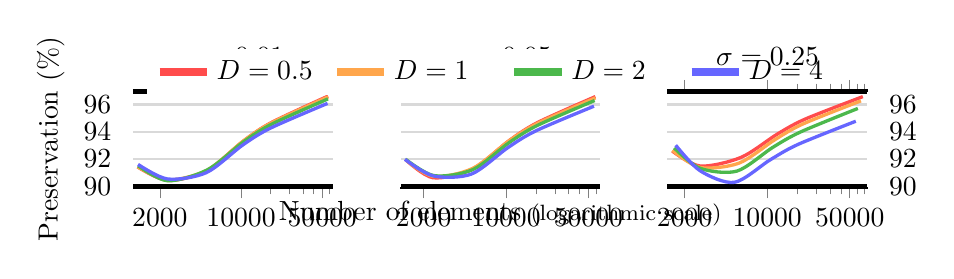
\begin{tikzpicture}
\begin{scope}[shift={(0.0\linewidth,0)}]
\begin{axis}[
 width=0.34\linewidth,height=0.23\linewidth,
 title=\normalsize\mbox{$\sigma=0.01$},
 xmode=log,enlarge x limits=0.025,
 ylabel=Preservation (\%),
 axis y line*=left,
 ymin=89.9630333333,ymax=96.9447983333,
 tick align=outside,
 x axis line style = ultra thick,y axis line style={white},
 xtick={2000,10000,50000},xticklabels={2000,10000,50000},
 minor xtick={18000,26000,34000,42000,58000,66000}, every y tick/.style={white},ymajorgrids,grid style={gray!30,thick}]
\addplot[very thick,mark=none,smooth,color=red!70] table[] {
	1286.178 91.41
	2338.11333333 90.4156666667
	5060.638 91.1263333333
	10480.9623333 93.3123333333
	18259.5173333 94.6713333333
	56146.2446667 96.6123333333
};
\addplot[very thick,mark=none,smooth,color=orange!70] table[] {
	1287.868 91.4186666667
	2339.78233333 90.4593333333
	5079.43933333 91.1566666667
	10512.7686667 93.33
	18294.7776667 94.65
	56228.2326667 96.555
};
\addplot[very thick,mark=none,smooth,color=green!60!black!70] table[] {
	1299.39333333 91.497
	2327.37133333 90.3943333333
	5117.85666667 91.1903333333
	10530.3903333 93.2626666667
	18304.1026667 94.5473333333
	56051.353 96.407
};
\addplot[very thick,mark=none,smooth,color=blue!60!] table[] {
	1297.967 91.5946666667
	2329.49466667 90.524
	5019.41733333 90.9893333333
	10373.4046667 93.0296666667
	18062.391 94.2743333333
	55540.5183333 96.0763333333
};
!\end{axis}
\end{scope}
\begin{scope}[shift={(0.28\linewidth,0)}]
\begin{axis}[
 width=0.34\linewidth,height=0.23\linewidth,
 title=\normalsize\mbox{$\sigma=0.05$},
 xmode=log,enlarge x limits=0.025,
 xlabel=Number of elements \footnotesize(logarithmic scale),x label style={at={(axis description cs:0.5,-0.05)},anchor=north},
 yticklabels={},
 legend style={at={(0.55,1.45)},legend style={text width=4em},legend style={draw=none},anchor=north,legend columns=-1},
 axis y line*=left,
 ymin=89.9630333333,ymax=96.9447983333,
 tick align=outside,
 x axis line style = ultra thick,y axis line style={white},
 xtick={2000,10000,50000},xticklabels={2000,10000,50000},
 minor xtick={18000,26000,34000,42000,58000,66000}, every y tick/.style={white},ymajorgrids,grid style={gray!30,thick}]
\addlegendimage{line width=3pt,mark=none,red!70}
\addlegendentry{$D=0.5$}
\addlegendimage{line width=3pt,mark=none,orange!70}
\addlegendentry{$D=1$}
\addlegendimage{line width=3pt,mark=none,green!60!black!70}
\addlegendentry{$D=2$}
\addlegendimage{line width=3pt,mark=none,blue!60!}
\addlegendentry{$D=4$}
\addplot[very thick,mark=none,smooth,color=red!70] table[] {
	1402.64766667 91.9493333333
	2398.12266667 90.616
	5190.80333333 91.2553333333
	10683.699 93.3583333333
	18660.8343333 94.6833333333
	57378.944 96.5756666667
};
\addplot[very thick,mark=none,smooth,color=orange!70] table[] {
	1402.59766667 91.9443333333
	2419.20233333 90.7136666667
	5204.22733333 91.2983333333
	10707.4293333 93.35
	18670.1523333 94.6266666667
	57488.2726667 96.4856666667
};
\addplot[very thick,mark=none,smooth,color=green!60!black!70] table[] {
	1400.94966667 91.9796666667
	2443.80233333 90.7723333333
	5218.954 91.2083333333
	10668.4646667 93.205
	18483.2026667 94.4606666667
	56547.8526667 96.2876666667
};
\addplot[very thick,mark=none,smooth,color=blue!60!] table[] {
	1386.54 91.9713333333
	2412.582 90.7493333333
	5078.19633333 90.8846666667
	10451.0006667 92.849
	18152.829 94.0823333333
	55798.5793333 95.87
};
!\end{axis}
\end{scope}
\begin{scope}[shift={(0.56\linewidth,0)}]
\begin{axis}[
 width=0.34\linewidth,height=0.23\linewidth,
 title=\normalsize\mbox{$\sigma=0.25$},
 xmode=log,enlarge x limits=0.025,
 axis y line*=right,
 ymin=89.9630333333,ymax=96.9447983333,
 tick align=outside,
 x axis line style = ultra thick,y axis line style={white},
 xtick={2000,10000,50000},xticklabels={2000,10000,50000},
 minor xtick={18000,26000,34000,42000,58000,66000}, every y tick/.style={white},ymajorgrids,grid style={gray!30,thick}]
\addplot[very thick,mark=none,smooth,color=red!70] table[] {
	1570.67133333 92.5796666667
	2706.189 91.476
	6003.85266667 92.1096666667
	12189.182 93.8243333333
	21086.423 94.9326666667
	64500.948 96.5733333333
};
\addplot[very thick,mark=none,smooth,color=orange!70] table[] {
	1576.92233333 92.63
	2694.657 91.373
	5761.26466667 91.687
	11659.3953333 93.42
	20235.336 94.5796666667
	62185.5713333 96.262
};
\addplot[very thick,mark=none,smooth,color=green!60!black!70] table[] {
	1630.739 92.8083333333
	2693.75533333 91.3153333333
	5525.561 91.1013333333
	11109.2813333 92.838
	19145.2023333 93.9766666667
	58572.3666667 95.7046666667
};
\addplot[very thick,mark=none,smooth,color=blue!60!] table[] {
	1680.32233333 93.006
	2707.413 91.1243333333
	5279.23033333 90.2796666667
	10616.6283333 91.937
	18309.9606667 93.0703333333
	56245.1786667 94.7656666667
};
!\end{axis}
\end{scope}
\end{tikzpicture}
\end{center}
\caption{Element preservation results using mesh remodelling - Eppler 545 airfoil}\centering\sffamily\footnotesize
Average of thirty optimisation scenarios\end{figure}

\begin{figure}[!h]
\begin{center}
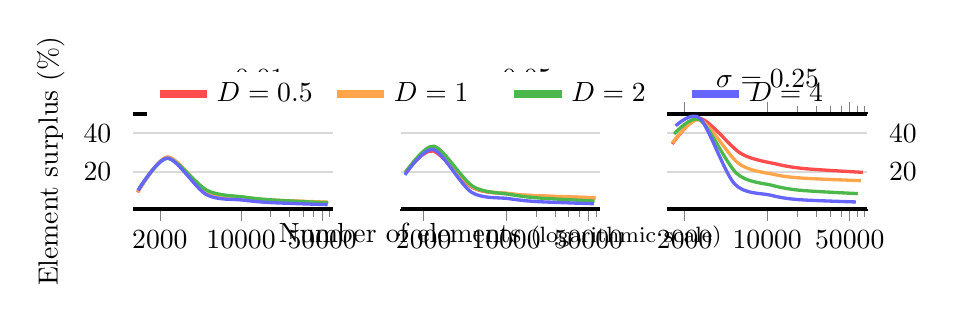
\begin{tikzpicture}
\begin{scope}[shift={(0.0\linewidth,0)}]
\begin{axis}[
 width=0.34\linewidth,height=0.23\linewidth,
 title=\normalsize\mbox{$\sigma=0.01$},
 xmode=log,enlarge x limits=0.025,
 ylabel=Element surplus (\%),
 axis y line*=left,
 ymin=0.839814325036,ymax=50.0990448367,
 tick align=outside,
 x axis line style = ultra thick,y axis line style={white},
 xtick={2000,10000,50000},xticklabels={2000,10000,50000},
 minor xtick={18000,26000,34000,42000,58000,66000}, every y tick/.style={white},ymajorgrids,grid style={gray!30,thick}]
\addplot[very thick,mark=none,smooth,color=red!70] table[] {
	1286.178 9.46363433653
	2338.11333333 27.6288977557
	5060.638 9.18724301441
	10480.9623333 6.54053412093
	18259.5173333 5.27945447888
	56146.2446667 4.19791849298
};
\addplot[very thick,mark=none,smooth,color=orange!70] table[] {
	1287.868 9.60746632714
	2339.78233333 27.720002249
	5079.43933333 9.59289656079
	10512.7686667 6.86385020909
	18294.7776667 5.48275605527
	56228.2326667 4.35007433158
};
\addplot[very thick,mark=none,smooth,color=green!60!black!70] table[] {
	1299.39333333 10.5883607862
	2327.37133333 27.042531988
	5117.85666667 10.4217807273
	10530.3903333 7.04297706014
	18304.1026667 5.5365214914
	56051.353 4.02181563503
};
\addplot[very thick,mark=none,smooth,color=blue!60!] table[] {
	1297.967 10.4669688557
	2329.49466667 27.1584368456
	5019.41733333 8.29787472753
	10373.4046667 5.44719451231
	18062.391 4.14287718289
	55540.5183333 3.07379303305
};
!\end{axis}
\end{scope}
\begin{scope}[shift={(0.28\linewidth,0)}]
\begin{axis}[
 width=0.34\linewidth,height=0.23\linewidth,
 title=\normalsize\mbox{$\sigma=0.05$},
 xmode=log,enlarge x limits=0.025,
 xlabel=Number of elements \footnotesize(logarithmic scale),x label style={at={(axis description cs:0.5,-0.05)},anchor=north},
 yticklabels={},
 legend style={at={(0.55,1.45)},legend style={text width=4em},legend style={draw=none},anchor=north,legend columns=-1},
 axis y line*=left,
 ymin=0.839814325036,ymax=50.0990448367,
 tick align=outside,
 x axis line style = ultra thick,y axis line style={white},
 xtick={2000,10000,50000},xticklabels={2000,10000,50000},
 minor xtick={18000,26000,34000,42000,58000,66000}, every y tick/.style={white},ymajorgrids,grid style={gray!30,thick}]
\addlegendimage{line width=3pt,mark=none,red!70}
\addlegendentry{$D=0.5$}
\addlegendimage{line width=3pt,mark=none,orange!70}
\addlegendentry{$D=1$}
\addlegendimage{line width=3pt,mark=none,green!60!black!70}
\addlegendentry{$D=2$}
\addlegendimage{line width=3pt,mark=none,blue!60!}
\addlegendentry{$D=4$}
\addplot[very thick,mark=none,smooth,color=red!70] table[] {
	1402.64766667 19.8985578356
	2398.12266667 30.872579304
	5190.80333333 11.9820033867
	10683.699 8.59910827089
	18660.8343333 7.60503919662
	57378.944 6.4940432487
};
\addplot[very thick,mark=none,smooth,color=orange!70] table[] {
	1402.59766667 19.8942838272
	2419.20233333 32.0229584676
	5204.22733333 12.2716014155
	10707.4293333 8.84032557203
	18670.1523333 7.6587701144
	57488.2726667 6.69695482121
};
\addplot[very thick,mark=none,smooth,color=green!60!black!70] table[] {
	1400.94966667 19.7534125108
	2443.80233333 33.3654525342
	5218.954 12.5893020739
	10668.4646667 8.4442522594
	18483.2026667 6.58075153012
	56547.8526667 4.95155622775
};
\addplot[very thick,mark=none,smooth,color=blue!60!] table[] {
	1386.54 18.5216717869
	2412.582 31.6616674831
	5078.19633333 9.55271515411
	10451.0006667 6.23374478619
	18152.829 4.67569890942
	55798.5793333 3.56092159416
};
!\end{axis}
\end{scope}
\begin{scope}[shift={(0.56\linewidth,0)}]
\begin{axis}[
 width=0.34\linewidth,height=0.23\linewidth,
 title=\normalsize\mbox{$\sigma=0.25$},
 xmode=log,enlarge x limits=0.025,
 axis y line*=right,
 ymin=0.839814325036,ymax=50.0990448367,
 tick align=outside,
 x axis line style = ultra thick,y axis line style={white},
 xtick={2000,10000,50000},xticklabels={2000,10000,50000},
 minor xtick={18000,26000,34000,42000,58000,66000}, every y tick/.style={white},ymajorgrids,grid style={gray!30,thick}]
\addplot[very thick,mark=none,smooth,color=red!70] table[] {
	1570.67133333 34.5323387715
	2706.189 47.6865690648
	6003.85266667 29.533117732
	12189.182 24.0115914702
	21086.423 21.710381548
	64500.948 19.8058475403
};
\addplot[very thick,mark=none,smooth,color=orange!70] table[] {
	1576.92233333 35.0677541903
	2694.657 47.057225913
	5761.26466667 24.2992817755
	11659.3953333 18.6215917415
	20235.336 16.7979256279
	62185.5713333 15.5052027819
};
\addplot[very thick,mark=none,smooth,color=green!60!black!70] table[] {
	1630.739 39.677300362
	2693.75533333 47.008018686
	5525.561 19.2139753066
	11109.2813333 13.0247836349
	19145.2023333 10.5056974719
	58572.3666667 8.79393634554
};
\addplot[very thick,mark=none,smooth,color=blue!60!] table[] {
	1680.32233333 43.9242498388
	2707.413 47.7533671932
	5279.23033333 13.8993913189
	10616.6283333 8.01257833908
	18309.9606667 5.68470047616
	56245.1786667 4.47135288948
};
!\end{axis}
\end{scope}
\end{tikzpicture}
\end{center}
\caption{Element surplus results on meshes from mesh remodelling - Eppler 545 airfoil}\centering\sffamily\footnotesize
Average of thirty optimisation scenarios\end{figure}

\begin{figure}[!h]
\begin{center}
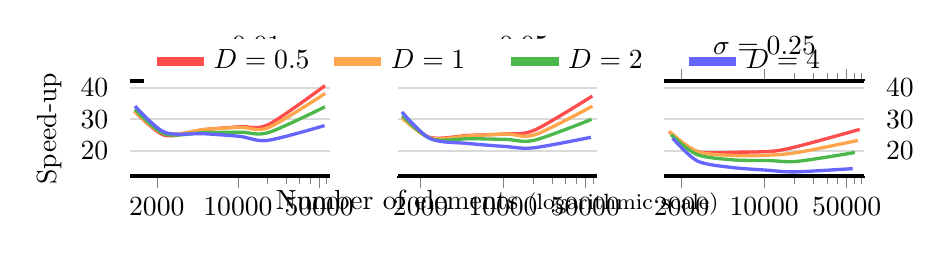
\begin{tikzpicture}
\begin{scope}[shift={(0.0\linewidth,0)}]
\begin{axis}[
 width=0.34\linewidth,height=0.23\linewidth,
 title=\normalsize\mbox{$\sigma=0.01$},
 xmode=log,enlarge x limits=0.025,
 ylabel=Speed-up,
 axis y line*=left,
 ymin=11.9003817799,ymax=42.0848725132,
 tick align=outside,
 x axis line style = ultra thick,y axis line style={white},
 xtick={2000,10000,50000},xticklabels={2000,10000,50000},
 minor xtick={18000,26000,34000,42000,58000,66000}, every y tick/.style={white},ymajorgrids,grid style={gray!30,thick}]
\addplot[very thick,mark=none,smooth,color=red!70] table[] {
	1286.178 32.6086427267
	2338.11333333 24.8843888071
	5060.638 26.6782075472
	10480.9623333 27.6003663004
	18259.5173333 28.2661821781
	56146.2446667 40.6475158116
};
\addplot[very thick,mark=none,smooth,color=orange!70] table[] {
	1287.868 32.5492102066
	2339.78233333 25.3067898153
	5079.43933333 26.7033994334
	10512.7686667 27.4133430352
	18294.7776667 27.3204179255
	56228.2326667 38.1584384826
};
\addplot[very thick,mark=none,smooth,color=green!60!black!70] table[] {
	1299.39333333 33.1945477076
	2327.37133333 25.3257556832
	5117.85666667 25.7034175604
	10530.3903333 25.8620216235
	18304.1026667 25.7630872961
	56051.353 33.9133495921
};
\addplot[very thick,mark=none,smooth,color=blue!60!] table[] {
	1297.967 34.1683673469
	2329.49466667 25.8619897959
	5019.41733333 25.3872879074
	10373.4046667 24.5336589337
	18062.391 23.2723626927
	55540.5183333 27.9554728541
};
!\end{axis}
\end{scope}
\begin{scope}[shift={(0.28\linewidth,0)}]
\begin{axis}[
 width=0.34\linewidth,height=0.23\linewidth,
 title=\normalsize\mbox{$\sigma=0.05$},
 xmode=log,enlarge x limits=0.025,
 xlabel=Number of elements \footnotesize(logarithmic scale),x label style={at={(axis description cs:0.5,-0.05)},anchor=north},
 yticklabels={},
 legend style={at={(0.55,1.45)},legend style={text width=4em},legend style={draw=none},anchor=north,legend columns=-1},
 axis y line*=left,
 ymin=11.9003817799,ymax=42.0848725132,
 tick align=outside,
 x axis line style = ultra thick,y axis line style={white},
 xtick={2000,10000,50000},xticklabels={2000,10000,50000},
 minor xtick={18000,26000,34000,42000,58000,66000}, every y tick/.style={white},ymajorgrids,grid style={gray!30,thick}]
\addlegendimage{line width=3pt,mark=none,red!70}
\addlegendentry{$D=0.5$}
\addlegendimage{line width=3pt,mark=none,orange!70}
\addlegendentry{$D=1$}
\addlegendimage{line width=3pt,mark=none,green!60!black!70}
\addlegendentry{$D=2$}
\addlegendimage{line width=3pt,mark=none,blue!60!}
\addlegendentry{$D=4$}
\addplot[very thick,mark=none,smooth,color=red!70] table[] {
	1402.64766667 30.7782909931
	2398.12266667 24.2023923445
	5190.80333333 24.8666904613
	10683.699 25.3229503253
	18660.8343333 26.5596102266
	57378.944 37.3333119605
};
\addplot[very thick,mark=none,smooth,color=orange!70] table[] {
	1402.59766667 30.3058555998
	2419.20233333 23.990040313
	5204.22733333 24.7057624113
	10707.4293333 25.2978824137
	18670.1523333 25.0523628261
	57488.2726667 34.1300859473
};
\addplot[very thick,mark=none,smooth,color=green!60!black!70] table[] {
	1400.94966667 31.1560490941
	2443.80233333 23.7423140108
	5218.954 23.8026135975
	10668.4646667 23.5768551945
	18483.2026667 23.3137352312
	56547.8526667 29.9408002571
};
\addplot[very thick,mark=none,smooth,color=blue!60!] table[] {
	1386.54 32.3078787879
	2412.582 23.8318021201
	5078.19633333 22.2837837838
	10451.0006667 21.3308292506
	18152.829 20.8983116481
	55798.5793333 24.2490056848
};
!\end{axis}
\end{scope}
\begin{scope}[shift={(0.56\linewidth,0)}]
\begin{axis}[
 width=0.34\linewidth,height=0.23\linewidth,
 title=\normalsize\mbox{$\sigma=0.25$},
 xmode=log,enlarge x limits=0.025,
 axis y line*=right,
 ymin=11.9003817799,ymax=42.0848725132,
 tick align=outside,
 x axis line style = ultra thick,y axis line style={white},
 xtick={2000,10000,50000},xticklabels={2000,10000,50000},
 minor xtick={18000,26000,34000,42000,58000,66000}, every y tick/.style={white},ymajorgrids,grid style={gray!30,thick}]
\addplot[very thick,mark=none,smooth,color=red!70] table[] {
	1570.67133333 26.1032448378
	2706.189 19.7699271797
	6003.85266667 19.523472483
	12189.182 19.8811327871
	21086.423 21.7471070002
	64500.948 26.7545088903
};
\addplot[very thick,mark=none,smooth,color=orange!70] table[] {
	1576.92233333 26.0264705882
	2694.657 19.7582612116
	5761.26466667 18.4457181849
	11659.3953333 18.62686711
	20235.336 19.5680109991
	62185.5713333 23.2406864818
};
\addplot[very thick,mark=none,smooth,color=green!60!black!70] table[] {
	1630.739 25.0561585654
	2693.75533333 18.7934518241
	5525.561 17.0711714556
	11109.2813333 16.8484469884
	19145.2023333 16.6140329032
	58572.3666667 19.4062526273
};
\addplot[very thick,mark=none,smooth,color=blue!60!] table[] {
	1680.32233333 23.9702031603
	2707.413 16.7641855808
	5279.23033333 14.686623927
	10616.6283333 13.7956605524
	18309.9606667 13.2692929243
	56245.1786667 14.2970665296
};
!\end{axis}
\end{scope}
\end{tikzpicture}
\end{center}
\caption{Speed-up results by mesh remodelling - Eppler 545 airfoil}\centering\sffamily\footnotesize
Average of thirty optimisation scenarios\end{figure}

\pagebreak
\subsubsection{Gottingen 702}
\vspace*{\fill} \begin{table}[!hp]
\begin{center}
\begin{tabular}{c|cc?c|c?c?c|c|c||c|c}
\multirow{2}{*}{\textbf{\large $\boldsymbol{\sigma}$}} & \multirow{2}{*}{\textbf{\large $\boldsymbol{I}$}} & \multirow{2}{*}{\textbf{\large $\boldsymbol{G}$}} & \multicolumn{2}{c?}{\textbf{\large Generation}} & \multirow{2}{*}{\textbf{\large $\boldsymbol{D}$}} & \multicolumn{5}{c}{\textbf{{\large Remodelling} }} \\\cline{4-5}\cline{7-11}
 & & & \textbf{\# Tri.} & \textbf{Time} & &\textbf{\# Tri.} & \textbf{Time} & \textbf{Preserv.} & \textbf{+ Tri.} & \textbf{Sp.-up} \\\toprule
\multirow{24}[11]{*}{.01} & \multirow{4}{*}{50} & \multirow{4}{*}{1} & \multirow{4}{*}{1122} & \multirow{4}{*}{1.72 ms} & .5 & 1338 & 0.06 ms & 91.61 \% & 19.24 \% & 30.37 \\\cline{6-11}
 & & & &  & 1 & 1343 & 0.06 ms & 91.64 \% & 19.64 \% & 30.38 \\\cline{6-11}
 & & & &  & 2 & 1342 & 0.06 ms & 91.67 \% & 19.54 \% & 31.04 \\\cline{6-11}
 & & & &  & 4 & 1326 & 0.05 ms & 91.74 \% & 18.14 \% & 32.30 \\\cmidrule[1.5pt]{2-11}
 & \multirow{4}{*}{100} & \multirow{4}{*}{2} & \multirow{4}{*}{1891} & \multirow{4}{*}{3.51 ms} & .5 & 2354 & 0.14 ms & 90.46 \% & 24.52 \% & 24.44 \\\cline{6-11}
 & & & &  & 1 & 2336 & 0.14 ms & 90.40 \% & 23.54 \% & 24.51 \\\cline{6-11}
 & & & &  & 2 & 2364 & 0.14 ms & 90.54 \% & 25.05 \% & 24.64 \\\cline{6-11}
 & & & &  & 4 & 2351 & 0.14 ms & 90.55 \% & 24.35 \% & 24.59 \\\cmidrule[1.5pt]{2-11}
 & \multirow{4}{*}{200} & \multirow{4}{*}{4} & \multirow{4}{*}{4598} & \multirow{4}{*}{9.63 ms} & .5 & 5224 & 0.39 ms & 91.33 \% & 13.61 \% & 24.89 \\\cline{6-11}
 & & & &  & 1 & 5220 & 0.39 ms & 91.31 \% & 13.52 \% & 24.71 \\\cline{6-11}
 & & & &  & 2 & 5178 & 0.41 ms & 91.15 \% & 12.61 \% & 23.72 \\\cline{6-11}
 & & & &  & 4 & 5045 & 0.43 ms & 90.83 \% & 9.72 \% & 22.46 \\\cmidrule[1.5pt]{2-11}
 & \multirow{4}{*}{300} & \multirow{4}{*}{6} & \multirow{4}{*}{9724} & \multirow{4}{*}{20.76 ms} & .5 & 10833 & 0.83 ms & 93.44 \% & 11.41 \% & 24.86 \\\cline{6-11}
 & & & &  & 1 & 10744 & 0.83 ms & 93.37 \% & 10.49 \% & 24.99 \\\cline{6-11}
 & & & &  & 2 & 10623 & 0.89 ms & 93.18 \% & 9.24 \% & 23.37 \\\cline{6-11}
 & & & &  & 4 & 10365 & 0.95 ms & 92.81 \% & 6.59 \% & 21.84 \\\cmidrule[1.5pt]{2-11}
 & \multirow{4}{*}{400} & \multirow{4}{*}{8} & \multirow{4}{*}{17197} & \multirow{4}{*}{36.76 ms} & .5 & 18899 & 1.52 ms & 94.76 \% & 9.90 \% & 24.24 \\\cline{6-11}
 & & & &  & 1 & 18702 & 1.58 ms & 94.66 \% & 8.75 \% & 23.31 \\\cline{6-11}
 & & & &  & 2 & 18427 & 1.70 ms & 94.44 \% & 7.15 \% & 21.61 \\\cline{6-11}
 & & & &  & 4 & 18010 & 1.85 ms & 94.03 \% & 4.73 \% & 19.89 \\\cmidrule[1.5pt]{2-11}
 & \multirow{4}{*}{700} & \multirow{4}{*}{14} & \multirow{4}{*}{53404} & \multirow{4}{*}{157.23 ms} & .5 & 57909 & 4.97 ms & 96.63 \% & 8.43 \% & 31.61 \\\cline{6-11}
 & & & &  & 1 & 57364 & 5.35 ms & 96.51 \% & 7.41 \% & 29.38 \\\cline{6-11}
 & & & &  & 2 & 56478 & 5.99 ms & 96.26 \% & 5.76 \% & 26.23 \\\cline{6-11}
 & & & &  & 4 & 55401 & 7.20 ms & 95.82 \% & 3.74 \% & 21.85\\\bottomrule
\end{tabular}\end{center}
\caption{Full results of mesh remodelling for $\sigma=0.01$ - Gottingen 702 airfoil}\centering\sffamily\footnotesize
Average of thirty optimisation scenarios\end{table}
 \vspace*{\fill}
\begin{table}[!hp]
\begin{center}
\begin{tabular}{c|cc?c|c?c?c|c|c||c|c}
\multirow{2}{*}{\textbf{\large $\boldsymbol{\sigma}$}} & \multirow{2}{*}{\textbf{\large $\boldsymbol{I}$}} & \multirow{2}{*}{\textbf{\large $\boldsymbol{G}$}} & \multicolumn{2}{c?}{\textbf{\large Generation}} & \multirow{2}{*}{\textbf{\large $\boldsymbol{D}$}} & \multicolumn{5}{c}{\textbf{{\large Remodelling} }} \\\cline{4-5}\cline{7-11}
 & & & \textbf{\# Tri.} & \textbf{Time} & &\textbf{\# Tri.} & \textbf{Time} & \textbf{Preserv.} & \textbf{+ Tri.} & \textbf{Sp.-up} \\\toprule
\multirow{24}[11]{*}{.05} & \multirow{4}{*}{50} & \multirow{4}{*}{1} & \multirow{4}{*}{1122} & \multirow{4}{*}{1.72 ms} & .5 & 1390 & 0.06 ms & 91.92 \% & 23.89 \% & 29.21 \\\cline{6-11}
 & & & &  & 1 & 1390 & 0.06 ms & 91.96 \% & 23.90 \% & 29.65 \\\cline{6-11}
 & & & &  & 2 & 1404 & 0.06 ms & 92.09 \% & 25.15 \% & 30.10 \\\cline{6-11}
 & & & &  & 4 & 1367 & 0.06 ms & 91.93 \% & 21.91 \% & 30.80 \\\cmidrule[1.5pt]{2-11}
 & \multirow{4}{*}{100} & \multirow{4}{*}{2} & \multirow{4}{*}{1892} & \multirow{4}{*}{3.51 ms} & .5 & 2433 & 0.15 ms & 90.75 \% & 28.64 \% & 23.93 \\\cline{6-11}
 & & & &  & 1 & 2448 & 0.15 ms & 90.82 \% & 29.43 \% & 24.14 \\\cline{6-11}
 & & & &  & 2 & 2451 & 0.15 ms & 90.82 \% & 29.58 \% & 23.97 \\\cline{6-11}
 & & & &  & 4 & 2382 & 0.15 ms & 90.60 \% & 25.91 \% & 23.40 \\\cmidrule[1.5pt]{2-11}
 & \multirow{4}{*}{200} & \multirow{4}{*}{4} & \multirow{4}{*}{4598} & \multirow{4}{*}{9.59 ms} & .5 & 5326 & 0.40 ms & 91.40 \% & 15.83 \% & 23.79 \\\cline{6-11}
 & & & &  & 1 & 5287 & 0.41 ms & 91.32 \% & 14.98 \% & 23.46 \\\cline{6-11}
 & & & &  & 2 & 5244 & 0.42 ms & 91.16 \% & 14.06 \% & 22.76 \\\cline{6-11}
 & & & &  & 4 & 5067 & 0.45 ms & 90.74 \% & 10.20 \% & 21.22 \\\cmidrule[1.5pt]{2-11}
 & \multirow{4}{*}{300} & \multirow{4}{*}{6} & \multirow{4}{*}{9724} & \multirow{4}{*}{20.47 ms} & .5 & 11021 & 0.85 ms & 93.49 \% & 13.34 \% & 23.95 \\\cline{6-11}
 & & & &  & 1 & 10911 & 0.87 ms & 93.39 \% & 12.21 \% & 23.59 \\\cline{6-11}
 & & & &  & 2 & 10719 & 0.93 ms & 93.14 \% & 10.23 \% & 21.95 \\\cline{6-11}
 & & & &  & 4 & 10410 & 1.01 ms & 92.70 \% & 7.06 \% & 20.35 \\\cmidrule[1.5pt]{2-11}
 & \multirow{4}{*}{400} & \multirow{4}{*}{8} & \multirow{4}{*}{17197} & \multirow{4}{*}{36.71 ms} & .5 & 19167 & 1.57 ms & 94.78 \% & 11.46 \% & 23.36 \\\cline{6-11}
 & & & &  & 1 & 18933 & 1.64 ms & 94.65 \% & 10.10 \% & 22.35 \\\cline{6-11}
 & & & &  & 2 & 18579 & 1.76 ms & 94.38 \% & 8.04 \% & 20.80 \\\cline{6-11}
 & & & &  & 4 & 18073 & 1.98 ms & 93.92 \% & 5.10 \% & 18.50 \\\cmidrule[1.5pt]{2-11}
 & \multirow{4}{*}{700} & \multirow{4}{*}{14} & \multirow{4}{*}{53397} & \multirow{4}{*}{156.93 ms} & .5 & 58808 & 5.18 ms & 96.62 \% & 10.13 \% & 30.29 \\\cline{6-11}
 & & & &  & 1 & 58120 & 5.66 ms & 96.47 \% & 8.84 \% & 27.73 \\\cline{6-11}
 & & & &  & 2 & 56917 & 6.32 ms & 96.20 \% & 6.59 \% & 24.82 \\\cline{6-11}
 & & & &  & 4 & 55583 & 7.72 ms & 95.70 \% & 4.09 \% & 20.33\\\bottomrule
\end{tabular}\end{center}
\caption{Full results of mesh remodelling for $\sigma=0.05$ - Gottingen 702 airfoil}\centering\sffamily\footnotesize
Average of thirty optimisation scenarios\end{table}

\begin{table}[!hp]
\begin{center}
\begin{tabular}{c|cc?c|c?c?c|c|c||c|c}
\multirow{2}{*}{\textbf{\large $\boldsymbol{\sigma}$}} & \multirow{2}{*}{\textbf{\large $\boldsymbol{I}$}} & \multirow{2}{*}{\textbf{\large $\boldsymbol{G}$}} & \multicolumn{2}{c?}{\textbf{\large Generation}} & \multirow{2}{*}{\textbf{\large $\boldsymbol{D}$}} & \multicolumn{5}{c}{\textbf{{\large Remodelling} }} \\\cline{4-5}\cline{7-11}
 & & & \textbf{\# Tri.} & \textbf{Time} & &\textbf{\# Tri.} & \textbf{Time} & \textbf{Preserv.} & \textbf{+ Tri.} & \textbf{Sp.-up} \\\toprule
\multirow{24}[13]{*}{.25} & \multirow{4}{*}{50} & \multirow{4}{*}{1} & \multirow{4}{*}{1121} & \multirow{4}{*}{1.72 ms} & .5 & 1543 & 0.07 ms & 92.55 \% & 37.72 \% & 25.41 \\\cline{6-11}
 & & & &  & 1 & 1541 & 0.07 ms & 92.55 \% & 37.55 \% & 25.34 \\\cline{6-11}
 & & & &  & 2 & 1600 & 0.07 ms & 92.75 \% & 42.79 \% & 25.10 \\\cline{6-11}
 & & & &  & 4 & 1619 & 0.07 ms & 92.83 \% & 44.47 \% & 23.83 \\\cmidrule[1.5pt]{2-11}
 & \multirow{4}{*}{100} & \multirow{4}{*}{2} & \multirow{4}{*}{1884} & \multirow{4}{*}{3.48 ms} & .5 & 2673 & 0.17 ms & 91.39 \% & 41.86 \% & 20.62 \\\cline{6-11}
 & & & &  & 1 & 2655 & 0.17 ms & 91.28 \% & 40.93 \% & 20.22 \\\cline{6-11}
 & & & &  & 2 & 2644 & 0.18 ms & 91.19 \% & 40.36 \% & 19.40 \\\cline{6-11}
 & & & &  & 4 & 2621 & 0.20 ms & 90.88 \% & 39.13 \% & 17.48 \\\cmidrule[1.5pt]{2-11}
 & \multirow{4}{*}{200} & \multirow{4}{*}{4} & \multirow{4}{*}{4593} & \multirow{4}{*}{9.31 ms} & .5 & 5964 & 0.49 ms & 92.06 \% & 29.85 \% & 19.16 \\\cline{6-11}
 & & & &  & 1 & 5720 & 0.49 ms & 91.65 \% & 24.52 \% & 18.84 \\\cline{6-11}
 & & & &  & 2 & 5442 & 0.54 ms & 91.02 \% & 18.46 \% & 17.35 \\\cline{6-11}
 & & & &  & 4 & 5228 & 0.62 ms & 90.21 \% & 13.81 \% & 15.01 \\\cmidrule[1.5pt]{2-11}
 & \multirow{4}{*}{300} & \multirow{4}{*}{6} & \multirow{4}{*}{9715} & \multirow{4}{*}{19.76 ms} & .5 & 12115 & 1.02 ms & 93.81 \% & 24.70 \% & 19.45 \\\cline{6-11}
 & & & &  & 1 & 11573 & 1.09 ms & 93.39 \% & 19.13 \% & 18.06 \\\cline{6-11}
 & & & &  & 2 & 10962 & 1.20 ms & 92.78 \% & 12.84 \% & 16.42 \\\cline{6-11}
 & & & &  & 4 & 10509 & 1.43 ms & 91.89 \% & 8.17 \% & 13.82 \\\cmidrule[1.5pt]{2-11}
 & \multirow{4}{*}{400} & \multirow{4}{*}{8} & \multirow{4}{*}{17179} & \multirow{4}{*}{36.42 ms} & .5 & 20964 & 1.80 ms & 94.92 \% & 22.03 \% & 20.23 \\\cline{6-11}
 & & & &  & 1 & 20060 & 2.01 ms & 94.54 \% & 16.77 \% & 18.09 \\\cline{6-11}
 & & & &  & 2 & 18906 & 2.28 ms & 93.95 \% & 10.05 \% & 16.01 \\\cline{6-11}
 & & & &  & 4 & 18156 & 2.81 ms & 93.04 \% & 5.68 \% & 12.95 \\\cmidrule[1.5pt]{2-11}
 & \multirow{4}{*}{700} & \multirow{4}{*}{14} & \multirow{4}{*}{53353} & \multirow{4}{*}{156.36 ms} & .5 & 64139 & 6.59 ms & 96.58 \% & 20.22 \% & 23.74 \\\cline{6-11}
 & & & &  & 1 & 61691 & 7.51 ms & 96.25 \% & 15.63 \% & 20.83 \\\cline{6-11}
 & & & &  & 2 & 57769 & 8.64 ms & 95.69 \% & 8.28 \% & 18.09 \\\cline{6-11}
 & & & &  & 4 & 55778 & 11.45 ms & 94.75 \% & 4.55 \% & 13.65\\\bottomrule
\end{tabular}\end{center}
\caption{Full results of mesh remodelling for $\sigma=0.25$ - Gottingen 702 airfoil}\centering\sffamily\footnotesize
Average of thirty optimisation scenarios\end{table}
 \newpage
\begin{figure}[!h]
\begin{center}
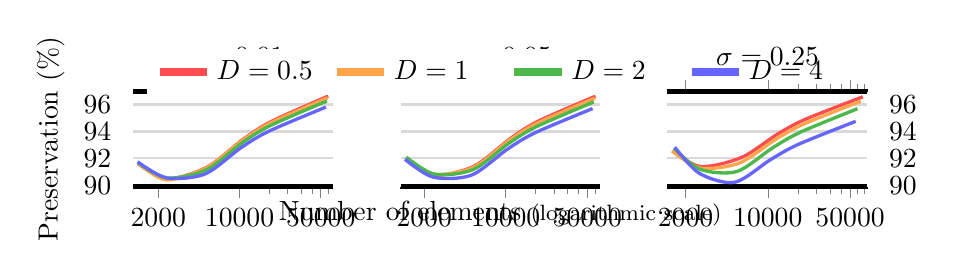
\begin{tikzpicture}
\begin{scope}[shift={(0.0\linewidth,0)}]
\begin{axis}[
 width=0.34\linewidth,height=0.23\linewidth,
 title=\normalsize\mbox{$\sigma=0.01$},
 xmode=log,enlarge x limits=0.025,
 ylabel=Preservation (\%),
 axis y line*=left,
 ymin=89.8934333333,ymax=96.9692783333,
 tick align=outside,
 x axis line style = ultra thick,y axis line style={white},
 xtick={2000,10000,50000},xticklabels={2000,10000,50000},
 minor xtick={18000,26000,34000,42000,58000,66000}, every y tick/.style={white},ymajorgrids,grid style={gray!30,thick}]
\addplot[very thick,mark=none,smooth,color=red!70] table[] {
	1338.169 91.6106666667
	2354.46133333 90.4623333333
	5223.685 91.333
	10833.4676667 93.441
	18899.4443333 94.7553333333
	57908.6903333 96.6323333333
};
\addplot[very thick,mark=none,smooth,color=orange!70] table[] {
	1342.68933333 91.6423333333
	2335.97666667 90.3963333333
	5219.54733333 91.3053333333
	10744.268 93.3693333333
	18701.6783333 94.6576666667
	57363.9423333 96.5106666667
};
\addplot[very thick,mark=none,smooth,color=green!60!black!70] table[] {
	1341.55466667 91.6686666667
	2364.473 90.539
	5177.77766667 91.147
	10622.5566667 93.1793333333
	18426.7493333 94.4386666667
	56478.105 96.264
};
\addplot[very thick,mark=none,smooth,color=blue!60!] table[] {
	1325.89833333 91.7403333333
	2351.403 90.5453333333
	5044.948 90.8346666667
	10364.783 92.8076666667
	18009.931 94.03
	55400.5926667 95.816
};
!\end{axis}
\end{scope}
\begin{scope}[shift={(0.28\linewidth,0)}]
\begin{axis}[
 width=0.34\linewidth,height=0.23\linewidth,
 title=\normalsize\mbox{$\sigma=0.05$},
 xmode=log,enlarge x limits=0.025,
 xlabel=Number of elements \footnotesize(logarithmic scale),x label style={at={(axis description cs:0.5,-0.05)},anchor=north},
 yticklabels={},
 legend style={at={(0.55,1.45)},legend style={text width=4em},legend style={draw=none},anchor=north,legend columns=-1},
 axis y line*=left,
 ymin=89.8934333333,ymax=96.9692783333,
 tick align=outside,
 x axis line style = ultra thick,y axis line style={white},
 xtick={2000,10000,50000},xticklabels={2000,10000,50000},
 minor xtick={18000,26000,34000,42000,58000,66000}, every y tick/.style={white},ymajorgrids,grid style={gray!30,thick}]
\addlegendimage{line width=3pt,mark=none,red!70}
\addlegendentry{$D=0.5$}
\addlegendimage{line width=3pt,mark=none,orange!70}
\addlegendentry{$D=1$}
\addlegendimage{line width=3pt,mark=none,green!60!black!70}
\addlegendentry{$D=2$}
\addlegendimage{line width=3pt,mark=none,blue!60!}
\addlegendentry{$D=4$}
\addplot[very thick,mark=none,smooth,color=red!70] table[] {
	1389.68533333 91.9216666667
	2433.372 90.7496666667
	5325.79166667 91.4043333333
	11020.5346667 93.489
	19167.226 94.7833333333
	58807.7403333 96.6226666667
};
\addplot[very thick,mark=none,smooth,color=orange!70] table[] {
	1389.75633333 91.9636666667
	2448.31266667 90.8216666667
	5286.70233333 91.3246666667
	10910.716 93.391
	18933.2866667 94.65
	58119.686 96.4736666667
};
\addplot[very thick,mark=none,smooth,color=green!60!black!70] table[] {
	1403.82133333 92.09
	2451.14066667 90.8156666667
	5244.49666667 91.161
	10718.5286667 93.1426666667
	18578.6793333 94.3823333333
	56916.5403333 96.201
};
\addplot[very thick,mark=none,smooth,color=blue!60!] table[] {
	1367.433 91.9293333333
	2381.80266667 90.602
	5067.15766667 90.7416666667
	10410.4156667 92.6993333333
	18073.1136667 93.9243333333
	55582.7506667 95.7033333333
};
!\end{axis}
\end{scope}
\begin{scope}[shift={(0.56\linewidth,0)}]
\begin{axis}[
 width=0.34\linewidth,height=0.23\linewidth,
 title=\normalsize\mbox{$\sigma=0.25$},
 xmode=log,enlarge x limits=0.025,
 axis y line*=right,
 ymin=89.8934333333,ymax=96.9692783333,
 tick align=outside,
 x axis line style = ultra thick,y axis line style={white},
 xtick={2000,10000,50000},xticklabels={2000,10000,50000},
 minor xtick={18000,26000,34000,42000,58000,66000}, every y tick/.style={white},ymajorgrids,grid style={gray!30,thick}]
\addplot[very thick,mark=none,smooth,color=red!70] table[] {
	1543.42233333 92.5516666667
	2672.75166667 91.3916666667
	5964.386 92.061
	12114.8056667 93.809
	20963.569 94.9156666667
	64139.478 96.5773333333
};
\addplot[very thick,mark=none,smooth,color=orange!70] table[] {
	1541.49866667 92.5463333333
	2655.24966667 91.2773333333
	5719.593 91.647
	11573.3 93.391
	20059.5583333 94.5443333333
	61690.9613333 96.25
};
\addplot[very thick,mark=none,smooth,color=green!60!black!70] table[] {
	1600.20833333 92.7543333333
	2644.44833333 91.191
	5441.57733333 91.0163333333
	10962.2683333 92.776
	18905.9213333 93.9466666667
	57769.0083333 95.6916666667
};
\addplot[very thick,mark=none,smooth,color=blue!60!] table[] {
	1619.01366667 92.8313333333
	2621.24833333 90.8813333333
	5227.893 90.2143333333
	10509.0943333 91.8943333333
	18155.882 93.0393333333
	55778.1196667 94.7523333333
};
!\end{axis}
\end{scope}
\end{tikzpicture}
\end{center}
\caption{Element preservation results using mesh remodelling - Gottingen 702 airfoil}\centering\sffamily\footnotesize
Average of thirty optimisation scenarios\end{figure}

\begin{figure}[!h]
\begin{center}
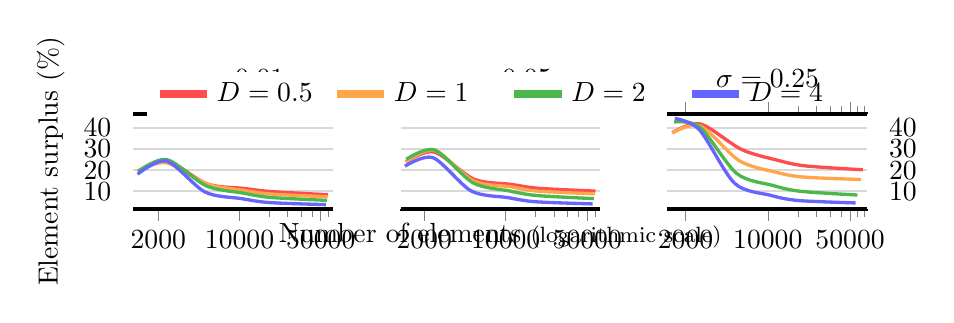
\begin{tikzpicture}
\begin{scope}[shift={(0.0\linewidth,0)}]
\begin{axis}[
 width=0.34\linewidth,height=0.23\linewidth,
 title=\normalsize\mbox{$\sigma=0.01$},
 xmode=log,enlarge x limits=0.025,
 ylabel=Element surplus (\%),
 axis y line*=left,
 ymin=1.70186602962,ymax=46.6055657785,
 tick align=outside,
 x axis line style = ultra thick,y axis line style={white},
 xtick={2000,10000,50000},xticklabels={2000,10000,50000},
 minor xtick={18000,26000,34000,42000,58000,66000}, every y tick/.style={white},ymajorgrids,grid style={gray!30,thick}]
\addplot[very thick,mark=none,smooth,color=red!70] table[] {
	1338.169 19.2370328282
	2354.46133333 24.5164123383
	5223.685 13.6058041046
	10833.4676667 11.40924121
	18899.4443333 9.90127996887
	57908.6903333 8.43475980583
};
\addplot[very thick,mark=none,smooth,color=orange!70] table[] {
	1342.68933333 19.6398153871
	2335.97666667 23.5388450519
	5219.54733333 13.5158172565
	10744.268 10.4919294604
	18701.6783333 8.75126009786
	57363.9423333 7.41471224139
};
\addplot[very thick,mark=none,smooth,color=green!60!black!70] table[] {
	1341.55466667 19.5387113512
	2364.473 25.0458824116
	5177.77766667 12.6074017282
	10622.5566667 9.24027415383
	18426.7493333 7.15253325343
	56478.105 5.75597055833
};
\addplot[very thick,mark=none,smooth,color=blue!60!] table[] {
	1325.89833333 18.1436598057
	2351.403 24.3546714386
	5044.948 9.71859409704
	10364.783 6.58938069193
	18009.931 4.72871234421
	55400.5926667 3.73831499782
};
!\end{axis}
\end{scope}
\begin{scope}[shift={(0.28\linewidth,0)}]
\begin{axis}[
 width=0.34\linewidth,height=0.23\linewidth,
 title=\normalsize\mbox{$\sigma=0.05$},
 xmode=log,enlarge x limits=0.025,
 xlabel=Number of elements \footnotesize(logarithmic scale),x label style={at={(axis description cs:0.5,-0.05)},anchor=north},
 yticklabels={},
 legend style={at={(0.55,1.45)},legend style={text width=4em},legend style={draw=none},anchor=north,legend columns=-1},
 axis y line*=left,
 ymin=1.70186602962,ymax=46.6055657785,
 tick align=outside,
 x axis line style = ultra thick,y axis line style={white},
 xtick={2000,10000,50000},xticklabels={2000,10000,50000},
 minor xtick={18000,26000,34000,42000,58000,66000}, every y tick/.style={white},ymajorgrids,grid style={gray!30,thick}]
\addlegendimage{line width=3pt,mark=none,red!70}
\addlegendentry{$D=0.5$}
\addlegendimage{line width=3pt,mark=none,orange!70}
\addlegendentry{$D=1$}
\addlegendimage{line width=3pt,mark=none,green!60!black!70}
\addlegendentry{$D=2$}
\addlegendimage{line width=3pt,mark=none,blue!60!}
\addlegendentry{$D=4$}
\addplot[very thick,mark=none,smooth,color=red!70] table[] {
	1389.68533333 23.8910724145
	2433.372 28.6410068942
	5325.79166667 15.8262567184
	11020.5346667 13.3356159331
	19167.226 11.4575545868
	58807.7403333 10.1324072375
};
\addplot[very thick,mark=none,smooth,color=orange!70] table[] {
	1389.75633333 23.8974020965
	2448.31266667 29.4308501256
	5286.70233333 14.9761350011
	10910.716 12.2062364062
	18933.2866667 10.0971957109
	58119.686 8.84385100989
};
\addplot[very thick,mark=none,smooth,color=green!60!black!70] table[] {
	1403.82133333 25.1513031716
	2451.14066667 29.5803532708
	5244.49666667 14.0582387167
	10718.5286667 10.229774242
	18578.6793333 8.03515156263
	56916.5403333 6.59065563499
};
\addplot[very thick,mark=none,smooth,color=blue!60!] table[] {
	1367.433 21.9072668909
	2381.80266667 25.9147772158
	5067.15766667 10.2014388594
	10410.4156667 7.06112792056
	18073.1136667 5.09528363967
	55582.7506667 4.09279623917
};
!\end{axis}
\end{scope}
\begin{scope}[shift={(0.56\linewidth,0)}]
\begin{axis}[
 width=0.34\linewidth,height=0.23\linewidth,
 title=\normalsize\mbox{$\sigma=0.25$},
 xmode=log,enlarge x limits=0.025,
 axis y line*=right,
 ymin=1.70186602962,ymax=46.6055657785,
 tick align=outside,
 x axis line style = ultra thick,y axis line style={white},
 xtick={2000,10000,50000},xticklabels={2000,10000,50000},
 minor xtick={18000,26000,34000,42000,58000,66000}, every y tick/.style={white},ymajorgrids,grid style={gray!30,thick}]
\addplot[very thick,mark=none,smooth,color=red!70] table[] {
	1543.42233333 37.7221533982
	2672.75166667 41.860579087
	5964.386 29.8461416995
	12114.8056667 24.7018644369
	20963.569 22.0282568008
	64139.478 20.2176493216
};
\addplot[very thick,mark=none,smooth,color=orange!70] table[] {
	1541.49866667 37.5505014076
	2655.24966667 40.9316323815
	5719.593 24.5169382299
	11573.3 19.1279602328
	20059.5583333 16.7660399625
	61690.9613333 15.6283553771
};
\addplot[very thick,mark=none,smooth,color=green!60!black!70] table[] {
	1600.20833333 42.7892630505
	2644.44833333 40.3583343005
	5441.57733333 18.464469183
	10962.2683333 12.8384009811
	18905.9213333 10.0507563154
	57769.0083333 8.27737615004
};
\addplot[very thick,mark=none,smooth,color=blue!60!] table[] {
	1619.01366667 44.4672943619
	2621.24833333 39.1269571113
	5227.893 13.8125089938
	10509.0943333 8.17372502436
	18155.882 5.68480162618
	55778.1196667 4.5458216842
};
!\end{axis}
\end{scope}
\end{tikzpicture}
\end{center}
\caption{Element surplus results on meshes from mesh remodelling - Gottingen 702 airfoil}\centering\sffamily\footnotesize
Average of thirty optimisation scenarios\end{figure}

\begin{figure}[!h]
\begin{center}
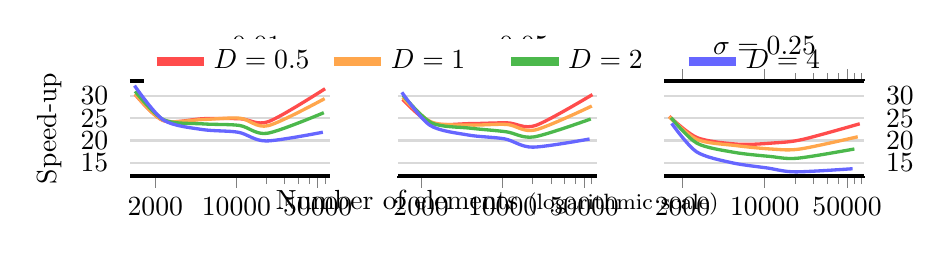
\begin{tikzpicture}
\begin{scope}[shift={(0.0\linewidth,0)}]
\begin{axis}[
 width=0.34\linewidth,height=0.23\linewidth,
 title=\normalsize\mbox{$\sigma=0.01$},
 xmode=log,enlarge x limits=0.025,
 ylabel=Speed-up,
 axis y line*=left,
 ymin=11.9849393289,ymax=33.3198899942,
 tick align=outside,
 x axis line style = ultra thick,y axis line style={white},
 xtick={2000,10000,50000},xticklabels={2000,10000,50000},
 minor xtick={18000,26000,34000,42000,58000,66000}, every y tick/.style={white},ymajorgrids,grid style={gray!30,thick}]
\addplot[very thick,mark=none,smooth,color=red!70] table[] {
	1338.169 30.3668430335
	2354.46133333 24.4443670151
	5223.685 24.8900370275
	10833.4676667 24.8648303393
	18899.4443333 24.2410472862
	57908.6903333 31.6099916234
};
\addplot[very thick,mark=none,smooth,color=orange!70] table[] {
	1342.68933333 30.3847058824
	2335.97666667 24.512695085
	5219.54733333 24.7112934941
	10744.268 24.9905312149
	18701.6783333 23.3148892084
	57363.9423333 29.3826407619
};
\addplot[very thick,mark=none,smooth,color=green!60!black!70] table[] {
	1341.55466667 31.0420673077
	2364.473 24.6447306792
	5177.77766667 23.7177320095
	10622.5566667 23.3685000375
	18426.7493333 21.6109946105
	56478.105 26.2297507702
};
\addplot[very thick,mark=none,smooth,color=blue!60!] table[] {
	1325.89833333 32.3039399625
	2351.403 24.5928955363
	5044.948 22.4625427417
	10364.783 21.8410828249
	18009.931 19.8889129376
	55400.5926667 21.8514224036
};
!\end{axis}
\end{scope}
\begin{scope}[shift={(0.28\linewidth,0)}]
\begin{axis}[
 width=0.34\linewidth,height=0.23\linewidth,
 title=\normalsize\mbox{$\sigma=0.05$},
 xmode=log,enlarge x limits=0.025,
 xlabel=Number of elements \footnotesize(logarithmic scale),x label style={at={(axis description cs:0.5,-0.05)},anchor=north},
 yticklabels={},
 legend style={at={(0.55,1.45)},legend style={text width=4em},legend style={draw=none},anchor=north,legend columns=-1},
 axis y line*=left,
 ymin=11.9849393289,ymax=33.3198899942,
 tick align=outside,
 x axis line style = ultra thick,y axis line style={white},
 xtick={2000,10000,50000},xticklabels={2000,10000,50000},
 minor xtick={18000,26000,34000,42000,58000,66000}, every y tick/.style={white},ymajorgrids,grid style={gray!30,thick}]
\addlegendimage{line width=3pt,mark=none,red!70}
\addlegendentry{$D=0.5$}
\addlegendimage{line width=3pt,mark=none,orange!70}
\addlegendentry{$D=1$}
\addlegendimage{line width=3pt,mark=none,green!60!black!70}
\addlegendentry{$D=2$}
\addlegendimage{line width=3pt,mark=none,blue!60!}
\addlegendentry{$D=4$}
\addplot[very thick,mark=none,smooth,color=red!70] table[] {
	1389.68533333 29.2139219015
	2433.372 23.9292699568
	5325.79166667 23.7874452072
	11020.5346667 23.9501150591
	19167.226 23.3643190496
	58807.7403333 30.2942660241
};
\addplot[very thick,mark=none,smooth,color=orange!70] table[] {
	1389.75633333 29.6502010339
	2448.31266667 24.1378756596
	5286.70233333 23.4557168488
	10910.716 23.5876387662
	18933.2866667 22.3460882974
	58119.686 27.7335764273
};
\addplot[very thick,mark=none,smooth,color=green!60!black!70] table[] {
	1403.82133333 30.0997084548
	2451.14066667 23.9674259681
	5244.49666667 22.7632766126
	10718.5286667 21.9502055407
	18578.6793333 20.8010349582
	56916.5403333 24.8204396879
};
\addplot[very thick,mark=none,smooth,color=blue!60!] table[] {
	1367.433 30.8001193317
	2381.80266667 23.4023576512
	5067.15766667 21.2214269903
	10410.4156667 20.3532316871
	18073.1136667 18.4980769554
	55582.7506667 20.3268440323
};
!\end{axis}
\end{scope}
\begin{scope}[shift={(0.56\linewidth,0)}]
\begin{axis}[
 width=0.34\linewidth,height=0.23\linewidth,
 title=\normalsize\mbox{$\sigma=0.25$},
 xmode=log,enlarge x limits=0.025,
 axis y line*=right,
 ymin=11.9849393289,ymax=33.3198899942,
 tick align=outside,
 x axis line style = ultra thick,y axis line style={white},
 xtick={2000,10000,50000},xticklabels={2000,10000,50000},
 minor xtick={18000,26000,34000,42000,58000,66000}, every y tick/.style={white},ymajorgrids,grid style={gray!30,thick}]
\addplot[very thick,mark=none,smooth,color=red!70] table[] {
	1543.42233333 25.4111549852
	2672.75166667 20.6213496448
	5964.386 19.157638508
	12114.8056667 19.4548587181
	20963.569 20.2277473341
	64139.478 23.7393722545
};
\addplot[very thick,mark=none,smooth,color=orange!70] table[] {
	1541.49866667 25.3361220472
	2655.24966667 20.2223297214
	5719.593 18.8411221256
	11573.3 18.0618811127
	20059.5583333 18.0882708385
	61690.9613333 20.8269176124
};
\addplot[very thick,mark=none,smooth,color=green!60!black!70] table[] {
	1600.20833333 25.1014139444
	2644.44833333 19.4038247308
	5441.57733333 17.3515712334
	10962.2683333 16.4244867426
	18905.9213333 16.0088789908
	57769.0083333 18.0872628141
};
\addplot[very thick,mark=none,smooth,color=blue!60!] table[] {
	1619.01366667 23.8347222222
	2621.24833333 17.4822683172
	5227.893 15.0107451781
	10509.0943333 13.8216134297
	18155.882 12.9525107876
	55778.1196667 13.6547966978
};
!\end{axis}
\end{scope}
\end{tikzpicture}
\end{center}
\caption{Speed-up results by mesh remodelling - Gottingen 702 airfoil}\centering\sffamily\footnotesize
Average of thirty optimisation scenarios\end{figure}

\pagebreak
	
\end{document}